% **************************************************************************************************************
% A Classic Thesis Style
% An Homage to The Elements of Typographic Style
%
% Copyright (C) 2015 André Miede http://www.miede.de
%
% If you like the style then I would appreciate a postcard. My address 
% can be found in the file ClassicThesis.pdf. A collection of the 
% postcards I received so far is available online at 
% http://postcards.miede.de
%
% License:
% This program is free software; you can redistribute it and/or modify
% it under the terms of the GNU General Public License as published by
% the Free Software Foundation; either version 2 of the License, or
% (at your option) any later version.
%
% This program is distributed in the hope that it will be useful,
% but WITHOUT ANY WARRANTY; without even the implied warranty of
% MERCHANTABILITY or FITNESS FOR A PARTICULAR PURPOSE.  See the
% GNU General Public License for more details.
%
% You should have received a copy of the GNU General Public License
% along with this program; see the file COPYING.  If not, write to
% the Free Software Foundation, Inc., 59 Temple Place - Suite 330,
% Boston, MA 02111-1307, USA.
%
% **************************************************************************************************************
\RequirePackage{fix-cm} % fix some latex issues see: http://texdoc.net/texmf-dist/doc/latex/base/fixltx2e.pdf
\documentclass[ twoside,openright,titlepage,numbers=noenddot,headinclude,%1headlines,% letterpaper a4paper
                footinclude=true,cleardoublepage=empty,abstractoff, % <--- obsolete, remove (todo)
                BCOR=5mm,paper=a4,fontsize=11pt,%11pt,a4paper,%
                ngerman,american,%
                ]{scrreprt}

%********************************************************************
% Note: Make all your adjustments in here
%*******************************************************
% ****************************************************************************************************
% classicthesis-config.tex 
% formerly known as loadpackages.sty, classicthesis-ldpkg.sty, and classicthesis-preamble.sty 
% Use it at the beginning of your ClassicThesis.tex, or as a LaTeX Preamble 
% in your ClassicThesis.{tex,lyx} with % ****************************************************************************************************
% classicthesis-config.tex 
% formerly known as loadpackages.sty, classicthesis-ldpkg.sty, and classicthesis-preamble.sty 
% Use it at the beginning of your ClassicThesis.tex, or as a LaTeX Preamble 
% in your ClassicThesis.{tex,lyx} with % ****************************************************************************************************
% classicthesis-config.tex 
% formerly known as loadpackages.sty, classicthesis-ldpkg.sty, and classicthesis-preamble.sty 
% Use it at the beginning of your ClassicThesis.tex, or as a LaTeX Preamble 
% in your ClassicThesis.{tex,lyx} with \input{classicthesis-config}
% ****************************************************************************************************  
% If you like the classicthesis, then I would appreciate a postcard. 
% My address can be found in the file ClassicThesis.pdf. A collection 
% of the postcards I received so far is available online at 
% http://postcards.miede.de
% ****************************************************************************************************


% ****************************************************************************************************
% 0. Set the encoding of your files. UTF-8 is the only sensible encoding nowadays. If you can't read
% äöüßáéçèê∂åëæƒÏ€ then change the encoding setting in your editor, not the line below. If your editor
% does not support utf8 use another editor!
% ****************************************************************************************************
\PassOptionsToPackage{utf8}{inputenc}
	\usepackage{inputenc}
\PassOptionsToPackage{dvipsnames}{xcolor}
\usepackage{xcolor}

% ****************************************************************************************************
% 1. Configure classicthesis for your needs here, e.g., remove "drafting" below 
% in order to deactivate the time-stamp on the pages
% ****************************************************************************************************
\PassOptionsToPackage{eulerchapternumbers,listings,%
					 pdfspacing,%floatperchapter,%linedheaders,%
					 beramono,eulermath,parts}{classicthesis}                                        
% ********************************************************************
% Available options for classicthesis.sty 
% (see ClassicThesis.pdf for more information):
% drafting
% parts nochapters linedheaders
% eulerchapternumbers beramono eulermath pdfspacing minionprospacing
% tocaligned dottedtoc manychapters
% listings floatperchapter subfig
% ********************************************************************


% ****************************************************************************************************
% 2. Personal data and user ad-hoc commands
% ****************************************************************************************************
\newcommand{\myTitle}{A Classic Thesis Style\xspace}
\newcommand{\mySubtitle}{An Homage to The Elements of Typographic Style\xspace}
\newcommand{\myDegree}{Doktor-Ingenieur (Dr.-Ing.)\xspace}
\newcommand{\myName}{André Miede\xspace}
\newcommand{\myProf}{Put name here\xspace}
\newcommand{\myOtherProf}{Put name here\xspace}
\newcommand{\mySupervisor}{Put name here\xspace}
\newcommand{\myFaculty}{Put data here\xspace}
\newcommand{\myDepartment}{Put data here\xspace}
\newcommand{\myUni}{Put data here\xspace}
\newcommand{\myLocation}{Saarbrücken\xspace}
\newcommand{\myTime}{September 2015\xspace}
\newcommand{\myVersion}{version 4.2\xspace}

% ********************************************************************
% Setup, finetuning, and useful commands
% ********************************************************************
\newcounter{dummy} % necessary for correct hyperlinks (to index, bib, etc.)
\newlength{\abcd} % for ab..z string length calculation
\providecommand{\mLyX}{L\kern-.1667em\lower.25em\hbox{Y}\kern-.125emX\@}
\newcommand{\ie}{i.\,e.}
\newcommand{\Ie}{I.\,e.}
\newcommand{\eg}{e.\,g.}
\newcommand{\Eg}{E.\,g.} 
\newcommand{\changed}[1]{#1} 
\newcommand{\new}[1]{#1}
\newcommand{\gb}{\textsf{GraphBench}\xspace}
\newcommand{\solver}[1]{\textsf{#1}}
\newcommand{\meanstd}[2]{\ensuremath{#1 \pm #2}}
\newcommand{\dataset}[1]{\textsf{#1}}
\newcommand{\tabledefaults}{\small\centering}
% ****************************************************************************************************


% ****************************************************************************************************
% 3. Loading some handy packages
% ****************************************************************************************************
% ******************************************************************** 
% Packages with options that might require adjustments
% ******************************************************************** 
%\PassOptionsToPackage{ngerman,american}{babel}   % change this to your language(s)
% Spanish languages need extra options in order to work with this template
%\PassOptionsToPackage{spanish,es-lcroman}{babel}
	\usepackage{babel}

\usepackage{csquotes}
\PassOptionsToPackage{%
    backend=biber,%
    style=apa,%
    natbib=true,%
    sorting=nyt%
}{biblatex}
    \usepackage{biblatex}

\PassOptionsToPackage{fleqn}{amsmath}       % math environments and more by the AMS 
    \usepackage{amsmath}
\usepackage{mathtools} % provides \coloneqq used by GraphBench
\usepackage{amssymb}
\providecommand{\R}{\mathbb{R}}
\providecommand{\X}{\mathcal{X}}
\providecommand{\Y}{\mathcal{Y}}
\providecommand{\D}{\mathcal{D}}
\providecommand{\T}{\mathcal{T}}
\DeclareMathOperator*{\argmin}{arg\,min}
\DeclareMathOperator*{\argmax}{arg\,max}
\usepackage{dsfont}
\usepackage{amsthm}
\newtheorem{theorem}{Theorem}[chapter]
\providecommand{\sR}{\mathbb{R}}
\providecommand{\train}{\mathcal{D}_{\text{train}}}
\providecommand{\test}{\mathcal{D}_{\text{test}}}

% ******************************************************************** 
% General useful packages
% ******************************************************************** 
\PassOptionsToPackage{T1}{fontenc} % T2A for cyrillics
    \usepackage{fontenc}     
\usepackage{textcomp} % fix warning with missing font shapes
\usepackage{scrhack} % fix warnings when using KOMA with listings package          
\usepackage{xspace} % to get the spacing after macros right  
\usepackage{mparhack} % get marginpar right
\usepackage[pass]{geometry} % to allow changing page geometry for specific pages (like Dedication)
%\usepackage[latest]{latexrelease} % will be used once available in more distributions (ISSUE #107)
\PassOptionsToPackage{printonlyused,smaller}{acronym} 
    \usepackage{acronym} % nice macros for handling all acronyms in the thesis
    %\renewcommand{\bflabel}[1]{{#1}\hfill} % fix the list of acronyms --> no longer working
    %\renewcommand*{\acsfont}[1]{\textsc{#1}} 
    \renewcommand*{\aclabelfont}[1]{\acsfont{#1}}

% Acronym wrapper macros translating glossaries (\gls) to acronym (\ac) commands
\newcommand{\gls}[1]{\ac{#1}}
\newcommand{\Gls}[1]{\Ac{#1}}
\newcommand{\glspl}[1]{\acp{#1}}
\newcommand{\Glspl}[1]{\Acp{#1}}

% Global acronym definitions using acrodef to ensure they are globally available
\acrodef{ai}[AI]{Artificial Intelligence}
\acrodef{api}[API]{Application Programming Interface}
\acrodef{as}[AS]{Algorithm Selection}
\acrodef{asf}[ASF]{Algorithm Selection Framework}
\acrodef{automl}[AutoML]{Automated Machine Learning}
\acrodef{bbo}[BBO]{Black-Box Optimisation}
\acrodef{bert}[BERT]{Bidirectional Encoder Representations from Transformers}
\acrodef{bertft}[BERT-FT]{fine-tuned BERT}
\acrodef{bo}[BO]{Bayesian Optimisation}
\acrodef{cg}[CG]{Closed Gap}
\acrodef{clg}[CG]{Clause Graph}
\acrodef{ci}[CI]{Continuous Integration}
\acrodef{clip}[CLIP]{Contrastive Language-Image Pre-training}
\acrodef{cnf}[CNF]{Conjunctive Normal Form}
\acrodef{dag}[DAG]{Directed Acyclic Graph}
\acrodef{dpll}[DPLL]{Davis-Putnam-Logemann-Loveland}
\acrodef{epm}[EPM]{Empirical Performance Model}
\acrodef{gnn}[GNN]{Graph Neural Network}
\acrodef{hpo}[HPO]{Hyperparameter Optimisation}
\acrodef{ice}[ICE]{Individual Conditional Expectation}
\acrodef{mit}[MIT]{Massachusetts Institute of Technology}
\acrodef{mlp}[MLP]{Multi-Layer Perceptron}
\acrodef{ood}[OOD]{Out-of-Distribution}
\acrodef{par}[PAR]{Penalised Average Runtime}
\acrodef{pddl}[PDDL]{Planning Domain Definition Language}
\acrodef{pep8}[PEP 8]{Python Enhancement Proposal 8}
\acrodef{rmse}[RMSE]{Root Mean Squared Error}
\acrodef{saps}[SAPS]{Scaling and Parameter Search}
\acrodef{sat}[SAT]{Propositional Satisfiability}
\acrodef{sbs}[SBS]{Single Best Solver}
\acrodef{vbs}[VBS]{Virtual Best Solver}
\usepackage{tikz}
\usetikzlibrary{shapes.geometric,arrows,arrows.meta,positioning,fit,backgrounds}
\definecolor{myyellow}{RGB}{251,210,87}
\definecolor{mypink}{RGB}{229,122,122}
\definecolor{mygray}{RGB}{96,96,96}
\definecolor{mypinkbg}{RGB}{240,195,195}
\definecolor{mypurple}{RGB}{155,142,246}
\usepackage{algorithm}
\usepackage{algorithmic}
\usepackage{placeins}
% ****************************************************************************************************


% ****************************************************************************************************
% 4. Setup floats: tables, (sub)figures, and captions
% ****************************************************************************************************
\usepackage{tabularx} % better tables
\usepackage{multirow}
    \setlength{\extrarowheight}{3pt} % increase table row height
\newcommand{\tableheadline}[1]{\multicolumn{1}{c}{\spacedlowsmallcaps{#1}}}
\newcommand{\myfloatalign}{\centering} % to be used with each float for alignment
\usepackage{caption}
% Thanks to cgnieder and Claus Lahiri
% http://tex.stackexchange.com/questions/69349/spacedlowsmallcaps-in-caption-label
% [REMOVED DUE TO OTHER PROBLEMS, SEE ISSUE #82]    
%\DeclareCaptionLabelFormat{smallcaps}{\bothIfFirst{#1}{~}\MakeTextLowercase{\textsc{#2}}}
%\captionsetup{font=small,labelformat=smallcaps} % format=hang,
\captionsetup{font=small} % format=hang,
\usepackage{subcaption}  
\usepackage{wrapfig}
% ****************************************************************************************************


% ****************************************************************************************************
% 5. Setup code listings
% ****************************************************************************************************
\usepackage{listings} 
%\lstset{emph={trueIndex,root},emphstyle=\color{BlueViolet}}%\underbar} % for special keywords
\lstset{language=[LaTeX]Tex,%C++,
    morekeywords={PassOptionsToPackage,selectlanguage},
    keywordstyle=\color{RoyalBlue},%\bfseries,
    basicstyle=\small\ttfamily,
    %identifierstyle=\color{NavyBlue},
    commentstyle=\color{Green}\ttfamily,
    stringstyle=\rmfamily,
    numbers=none,%left,%
    numberstyle=\scriptsize,%\tiny
    stepnumber=5,
    numbersep=8pt,
    showstringspaces=false,
    breaklines=true,
    %frameround=ftff,
    %frame=single,
    belowcaptionskip=.75\baselineskip
    %frame=L
} 
\lstdefinestyle{asfpython}{
    language=Python,
    basicstyle=\small\ttfamily,
    keywordstyle=\color{RoyalBlue},
    commentstyle=\color{Green}\ttfamily,
    stringstyle=\color{black},
    showstringspaces=false,
    breaklines=true
}
% ****************************************************************************************************             


% ****************************************************************************************************
% 6. PDFLaTeX, hyperreferences and citation backreferences
% ****************************************************************************************************
% ********************************************************************
% Using PDFLaTeX
% ********************************************************************
\PassOptionsToPackage{pdftex,hyperfootnotes=false,pdfpagelabels}{hyperref}
    \usepackage{hyperref}  % backref linktocpage pagebackref
    \usepackage{bookmark} % handles KOMA heading levels without bookmark gaps
    % Supply the English language hook without loading a second Babel dialect.
    \providecommand*{\extrasenglish}{}
    \usepackage[english,capitalise,nameinlink]{cleveref}
    % cleveref recognises "english", but Babel's main language is "american".
    % Restore English reference names when leaving the German abstract.
    \AtBeginDocument{\addto\extrasamerican{\extrasenglish}}
\pdfcompresslevel=9
\pdfadjustspacing=1 
\PassOptionsToPackage{pdftex}{graphicx}
    \usepackage{graphicx} 
\usepackage{pdfpages} % insert the supplied PDF cover without thesis margins
 

% ********************************************************************
% Hyperreferences
% ********************************************************************
\hypersetup{%
    %draft, % = no hyperlinking at all (useful in b/w printouts)
    colorlinks=true, linktocpage=true, pdfstartpage=3, pdfstartview=FitV,%
    % uncomment the following line if you want to have black links (e.g., for printing)
    %colorlinks=false, linktocpage=false, pdfstartpage=3, pdfstartview=FitV, pdfborder={0 0 0},%
    breaklinks=true, pdfpagemode=UseNone, pageanchor=true, pdfpagemode=UseOutlines,%
    plainpages=false, bookmarksnumbered, bookmarksopen=true, bookmarksopenlevel=1,%
    hypertexnames=true, pdfhighlight=/O,%nesting=true,%frenchlinks,%
    %urlcolor=webbrown, linkcolor=RoyalBlue, citecolor=webgreen, %pagecolor=RoyalBlue,%
    urlcolor=black, linkcolor=black, citecolor=black, %pagecolor=black,%
    pdftitle={\myTitle},%
    pdfauthor={\textcopyright\ \myName, \myUni, \myFaculty},%
    pdfsubject={},%
    pdfkeywords={},%
    pdfcreator={pdfLaTeX},%
    pdfproducer={LaTeX with hyperref and classicthesis}%
}   

% ********************************************************************
% Setup autoreferences
% ********************************************************************
% There are some issues regarding autorefnames
% http://www.ureader.de/msg/136221647.aspx
% http://www.tex.ac.uk/cgi-bin/texfaq2html?label=latexwords
% you have to redefine the makros for the 
% language you use, e.g., american, ngerman
% (as chosen when loading babel/AtBeginDocument)
% ********************************************************************
\makeatletter
\@ifpackageloaded{babel}%
    {%
       \addto\extrasamerican{%
			\renewcommand*{\figureautorefname}{Figure}%
			\renewcommand*{\tableautorefname}{Table}%
			\renewcommand*{\partautorefname}{Part}%
			\renewcommand*{\chapterautorefname}{Chapter}%
			\renewcommand*{\sectionautorefname}{Section}%
			\renewcommand*{\subsectionautorefname}{Section}%
			\renewcommand*{\subsubsectionautorefname}{Section}%     
                }%
       \addto\extrasngerman{% 
			\renewcommand*{\paragraphautorefname}{Absatz}%
			\renewcommand*{\subparagraphautorefname}{Unterabsatz}%
			\renewcommand*{\footnoteautorefname}{Fu\"snote}%
			\renewcommand*{\FancyVerbLineautorefname}{Zeile}%
			\renewcommand*{\theoremautorefname}{Theorem}%
			\renewcommand*{\appendixautorefname}{Anhang}%
			\renewcommand*{\equationautorefname}{Gleichung}%        
			\renewcommand*{\itemautorefname}{Punkt}%
                }%  
            % Fix to getting autorefs for subfigures right (thanks to Belinda Vogt for changing the definition)
            \providecommand{\subfigureautorefname}{\figureautorefname}%             
    }{\relax}
\makeatother


% ****************************************************************************************************
% 7. Last calls before the bar closes
% ****************************************************************************************************
% ********************************************************************
% Development Stuff
% ********************************************************************
\listfiles
%\PassOptionsToPackage{l2tabu,orthodox,abort}{nag}
%   \usepackage{nag}
%\PassOptionsToPackage{warning, all}{onlyamsmath}
%   \usepackage{onlyamsmath}

% ********************************************************************
% Last, but not least...
% ********************************************************************
\usepackage{classicthesis} 
% ****************************************************************************************************


% ****************************************************************************************************
% 8. Further adjustments (experimental)
% ****************************************************************************************************
% ********************************************************************
% Changing the text area
% ********************************************************************
%\linespread{1.05} % a bit more for Palatino
%\areaset[current]{312pt}{761pt} % 686 (factor 2.2) + 33 head + 42 head \the\footskip
%\setlength{\marginparwidth}{7em}%
%\setlength{\marginparsep}{2em}%

% ********************************************************************
% Using different fonts
% ********************************************************************
%\usepackage[oldstylenums]{kpfonts} % oldstyle notextcomp
%\usepackage[osf]{libertine}
%\usepackage[light,condensed,math]{iwona}
%\renewcommand{\sfdefault}{iwona}
%\usepackage{lmodern} % <-- no osf support :-(
%\usepackage{cfr-lm} % 
%\usepackage[urw-garamond]{mathdesign} <-- no osf support :-(
%\usepackage[default,osfigures]{opensans} % scale=0.95 
%\usepackage[sfdefault]{FiraSans}
% ****************************************************************************************************

% ****************************************************************************************************  
% If you like the classicthesis, then I would appreciate a postcard. 
% My address can be found in the file ClassicThesis.pdf. A collection 
% of the postcards I received so far is available online at 
% http://postcards.miede.de
% ****************************************************************************************************


% ****************************************************************************************************
% 0. Set the encoding of your files. UTF-8 is the only sensible encoding nowadays. If you can't read
% äöüßáéçèê∂åëæƒÏ€ then change the encoding setting in your editor, not the line below. If your editor
% does not support utf8 use another editor!
% ****************************************************************************************************
\PassOptionsToPackage{utf8}{inputenc}
	\usepackage{inputenc}
\PassOptionsToPackage{dvipsnames}{xcolor}
\usepackage{xcolor}

% ****************************************************************************************************
% 1. Configure classicthesis for your needs here, e.g., remove "drafting" below 
% in order to deactivate the time-stamp on the pages
% ****************************************************************************************************
\PassOptionsToPackage{eulerchapternumbers,listings,%
					 pdfspacing,%floatperchapter,%linedheaders,%
					 beramono,eulermath,parts}{classicthesis}                                        
% ********************************************************************
% Available options for classicthesis.sty 
% (see ClassicThesis.pdf for more information):
% drafting
% parts nochapters linedheaders
% eulerchapternumbers beramono eulermath pdfspacing minionprospacing
% tocaligned dottedtoc manychapters
% listings floatperchapter subfig
% ********************************************************************


% ****************************************************************************************************
% 2. Personal data and user ad-hoc commands
% ****************************************************************************************************
\newcommand{\myTitle}{A Classic Thesis Style\xspace}
\newcommand{\mySubtitle}{An Homage to The Elements of Typographic Style\xspace}
\newcommand{\myDegree}{Doktor-Ingenieur (Dr.-Ing.)\xspace}
\newcommand{\myName}{André Miede\xspace}
\newcommand{\myProf}{Put name here\xspace}
\newcommand{\myOtherProf}{Put name here\xspace}
\newcommand{\mySupervisor}{Put name here\xspace}
\newcommand{\myFaculty}{Put data here\xspace}
\newcommand{\myDepartment}{Put data here\xspace}
\newcommand{\myUni}{Put data here\xspace}
\newcommand{\myLocation}{Saarbrücken\xspace}
\newcommand{\myTime}{September 2015\xspace}
\newcommand{\myVersion}{version 4.2\xspace}

% ********************************************************************
% Setup, finetuning, and useful commands
% ********************************************************************
\newcounter{dummy} % necessary for correct hyperlinks (to index, bib, etc.)
\newlength{\abcd} % for ab..z string length calculation
\providecommand{\mLyX}{L\kern-.1667em\lower.25em\hbox{Y}\kern-.125emX\@}
\newcommand{\ie}{i.\,e.}
\newcommand{\Ie}{I.\,e.}
\newcommand{\eg}{e.\,g.}
\newcommand{\Eg}{E.\,g.} 
\newcommand{\changed}[1]{#1} 
\newcommand{\new}[1]{#1}
\newcommand{\gb}{\textsf{GraphBench}\xspace}
\newcommand{\solver}[1]{\textsf{#1}}
\newcommand{\meanstd}[2]{\ensuremath{#1 \pm #2}}
\newcommand{\dataset}[1]{\textsf{#1}}
\newcommand{\tabledefaults}{\small\centering}
% ****************************************************************************************************


% ****************************************************************************************************
% 3. Loading some handy packages
% ****************************************************************************************************
% ******************************************************************** 
% Packages with options that might require adjustments
% ******************************************************************** 
%\PassOptionsToPackage{ngerman,american}{babel}   % change this to your language(s)
% Spanish languages need extra options in order to work with this template
%\PassOptionsToPackage{spanish,es-lcroman}{babel}
	\usepackage{babel}

\usepackage{csquotes}
\PassOptionsToPackage{%
    backend=biber,%
    style=apa,%
    natbib=true,%
    sorting=nyt%
}{biblatex}
    \usepackage{biblatex}

\PassOptionsToPackage{fleqn}{amsmath}       % math environments and more by the AMS 
    \usepackage{amsmath}
\usepackage{mathtools} % provides \coloneqq used by GraphBench
\usepackage{amssymb}
\providecommand{\R}{\mathbb{R}}
\providecommand{\X}{\mathcal{X}}
\providecommand{\Y}{\mathcal{Y}}
\providecommand{\D}{\mathcal{D}}
\providecommand{\T}{\mathcal{T}}
\DeclareMathOperator*{\argmin}{arg\,min}
\DeclareMathOperator*{\argmax}{arg\,max}
\usepackage{dsfont}
\usepackage{amsthm}
\newtheorem{theorem}{Theorem}[chapter]
\providecommand{\sR}{\mathbb{R}}
\providecommand{\train}{\mathcal{D}_{\text{train}}}
\providecommand{\test}{\mathcal{D}_{\text{test}}}

% ******************************************************************** 
% General useful packages
% ******************************************************************** 
\PassOptionsToPackage{T1}{fontenc} % T2A for cyrillics
    \usepackage{fontenc}     
\usepackage{textcomp} % fix warning with missing font shapes
\usepackage{scrhack} % fix warnings when using KOMA with listings package          
\usepackage{xspace} % to get the spacing after macros right  
\usepackage{mparhack} % get marginpar right
\usepackage[pass]{geometry} % to allow changing page geometry for specific pages (like Dedication)
%\usepackage[latest]{latexrelease} % will be used once available in more distributions (ISSUE #107)
\PassOptionsToPackage{printonlyused,smaller}{acronym} 
    \usepackage{acronym} % nice macros for handling all acronyms in the thesis
    %\renewcommand{\bflabel}[1]{{#1}\hfill} % fix the list of acronyms --> no longer working
    %\renewcommand*{\acsfont}[1]{\textsc{#1}} 
    \renewcommand*{\aclabelfont}[1]{\acsfont{#1}}

% Acronym wrapper macros translating glossaries (\gls) to acronym (\ac) commands
\newcommand{\gls}[1]{\ac{#1}}
\newcommand{\Gls}[1]{\Ac{#1}}
\newcommand{\glspl}[1]{\acp{#1}}
\newcommand{\Glspl}[1]{\Acp{#1}}

% Global acronym definitions using acrodef to ensure they are globally available
\acrodef{ai}[AI]{Artificial Intelligence}
\acrodef{api}[API]{Application Programming Interface}
\acrodef{as}[AS]{Algorithm Selection}
\acrodef{asf}[ASF]{Algorithm Selection Framework}
\acrodef{automl}[AutoML]{Automated Machine Learning}
\acrodef{bbo}[BBO]{Black-Box Optimisation}
\acrodef{bert}[BERT]{Bidirectional Encoder Representations from Transformers}
\acrodef{bertft}[BERT-FT]{fine-tuned BERT}
\acrodef{bo}[BO]{Bayesian Optimisation}
\acrodef{cg}[CG]{Closed Gap}
\acrodef{clg}[CG]{Clause Graph}
\acrodef{ci}[CI]{Continuous Integration}
\acrodef{clip}[CLIP]{Contrastive Language-Image Pre-training}
\acrodef{cnf}[CNF]{Conjunctive Normal Form}
\acrodef{dag}[DAG]{Directed Acyclic Graph}
\acrodef{dpll}[DPLL]{Davis-Putnam-Logemann-Loveland}
\acrodef{epm}[EPM]{Empirical Performance Model}
\acrodef{gnn}[GNN]{Graph Neural Network}
\acrodef{hpo}[HPO]{Hyperparameter Optimisation}
\acrodef{ice}[ICE]{Individual Conditional Expectation}
\acrodef{mit}[MIT]{Massachusetts Institute of Technology}
\acrodef{mlp}[MLP]{Multi-Layer Perceptron}
\acrodef{ood}[OOD]{Out-of-Distribution}
\acrodef{par}[PAR]{Penalised Average Runtime}
\acrodef{pddl}[PDDL]{Planning Domain Definition Language}
\acrodef{pep8}[PEP 8]{Python Enhancement Proposal 8}
\acrodef{rmse}[RMSE]{Root Mean Squared Error}
\acrodef{saps}[SAPS]{Scaling and Parameter Search}
\acrodef{sat}[SAT]{Propositional Satisfiability}
\acrodef{sbs}[SBS]{Single Best Solver}
\acrodef{vbs}[VBS]{Virtual Best Solver}
\usepackage{tikz}
\usetikzlibrary{shapes.geometric,arrows,arrows.meta,positioning,fit,backgrounds}
\definecolor{myyellow}{RGB}{251,210,87}
\definecolor{mypink}{RGB}{229,122,122}
\definecolor{mygray}{RGB}{96,96,96}
\definecolor{mypinkbg}{RGB}{240,195,195}
\definecolor{mypurple}{RGB}{155,142,246}
\usepackage{algorithm}
\usepackage{algorithmic}
\usepackage{placeins}
% ****************************************************************************************************


% ****************************************************************************************************
% 4. Setup floats: tables, (sub)figures, and captions
% ****************************************************************************************************
\usepackage{tabularx} % better tables
\usepackage{multirow}
    \setlength{\extrarowheight}{3pt} % increase table row height
\newcommand{\tableheadline}[1]{\multicolumn{1}{c}{\spacedlowsmallcaps{#1}}}
\newcommand{\myfloatalign}{\centering} % to be used with each float for alignment
\usepackage{caption}
% Thanks to cgnieder and Claus Lahiri
% http://tex.stackexchange.com/questions/69349/spacedlowsmallcaps-in-caption-label
% [REMOVED DUE TO OTHER PROBLEMS, SEE ISSUE #82]    
%\DeclareCaptionLabelFormat{smallcaps}{\bothIfFirst{#1}{~}\MakeTextLowercase{\textsc{#2}}}
%\captionsetup{font=small,labelformat=smallcaps} % format=hang,
\captionsetup{font=small} % format=hang,
\usepackage{subcaption}  
\usepackage{wrapfig}
% ****************************************************************************************************


% ****************************************************************************************************
% 5. Setup code listings
% ****************************************************************************************************
\usepackage{listings} 
%\lstset{emph={trueIndex,root},emphstyle=\color{BlueViolet}}%\underbar} % for special keywords
\lstset{language=[LaTeX]Tex,%C++,
    morekeywords={PassOptionsToPackage,selectlanguage},
    keywordstyle=\color{RoyalBlue},%\bfseries,
    basicstyle=\small\ttfamily,
    %identifierstyle=\color{NavyBlue},
    commentstyle=\color{Green}\ttfamily,
    stringstyle=\rmfamily,
    numbers=none,%left,%
    numberstyle=\scriptsize,%\tiny
    stepnumber=5,
    numbersep=8pt,
    showstringspaces=false,
    breaklines=true,
    %frameround=ftff,
    %frame=single,
    belowcaptionskip=.75\baselineskip
    %frame=L
} 
\lstdefinestyle{asfpython}{
    language=Python,
    basicstyle=\small\ttfamily,
    keywordstyle=\color{RoyalBlue},
    commentstyle=\color{Green}\ttfamily,
    stringstyle=\color{black},
    showstringspaces=false,
    breaklines=true
}
% ****************************************************************************************************             


% ****************************************************************************************************
% 6. PDFLaTeX, hyperreferences and citation backreferences
% ****************************************************************************************************
% ********************************************************************
% Using PDFLaTeX
% ********************************************************************
\PassOptionsToPackage{pdftex,hyperfootnotes=false,pdfpagelabels}{hyperref}
    \usepackage{hyperref}  % backref linktocpage pagebackref
    \usepackage{bookmark} % handles KOMA heading levels without bookmark gaps
    % Supply the English language hook without loading a second Babel dialect.
    \providecommand*{\extrasenglish}{}
    \usepackage[english,capitalise,nameinlink]{cleveref}
    % cleveref recognises "english", but Babel's main language is "american".
    % Restore English reference names when leaving the German abstract.
    \AtBeginDocument{\addto\extrasamerican{\extrasenglish}}
\pdfcompresslevel=9
\pdfadjustspacing=1 
\PassOptionsToPackage{pdftex}{graphicx}
    \usepackage{graphicx} 
\usepackage{pdfpages} % insert the supplied PDF cover without thesis margins
 

% ********************************************************************
% Hyperreferences
% ********************************************************************
\hypersetup{%
    %draft, % = no hyperlinking at all (useful in b/w printouts)
    colorlinks=true, linktocpage=true, pdfstartpage=3, pdfstartview=FitV,%
    % uncomment the following line if you want to have black links (e.g., for printing)
    %colorlinks=false, linktocpage=false, pdfstartpage=3, pdfstartview=FitV, pdfborder={0 0 0},%
    breaklinks=true, pdfpagemode=UseNone, pageanchor=true, pdfpagemode=UseOutlines,%
    plainpages=false, bookmarksnumbered, bookmarksopen=true, bookmarksopenlevel=1,%
    hypertexnames=true, pdfhighlight=/O,%nesting=true,%frenchlinks,%
    %urlcolor=webbrown, linkcolor=RoyalBlue, citecolor=webgreen, %pagecolor=RoyalBlue,%
    urlcolor=black, linkcolor=black, citecolor=black, %pagecolor=black,%
    pdftitle={\myTitle},%
    pdfauthor={\textcopyright\ \myName, \myUni, \myFaculty},%
    pdfsubject={},%
    pdfkeywords={},%
    pdfcreator={pdfLaTeX},%
    pdfproducer={LaTeX with hyperref and classicthesis}%
}   

% ********************************************************************
% Setup autoreferences
% ********************************************************************
% There are some issues regarding autorefnames
% http://www.ureader.de/msg/136221647.aspx
% http://www.tex.ac.uk/cgi-bin/texfaq2html?label=latexwords
% you have to redefine the makros for the 
% language you use, e.g., american, ngerman
% (as chosen when loading babel/AtBeginDocument)
% ********************************************************************
\makeatletter
\@ifpackageloaded{babel}%
    {%
       \addto\extrasamerican{%
			\renewcommand*{\figureautorefname}{Figure}%
			\renewcommand*{\tableautorefname}{Table}%
			\renewcommand*{\partautorefname}{Part}%
			\renewcommand*{\chapterautorefname}{Chapter}%
			\renewcommand*{\sectionautorefname}{Section}%
			\renewcommand*{\subsectionautorefname}{Section}%
			\renewcommand*{\subsubsectionautorefname}{Section}%     
                }%
       \addto\extrasngerman{% 
			\renewcommand*{\paragraphautorefname}{Absatz}%
			\renewcommand*{\subparagraphautorefname}{Unterabsatz}%
			\renewcommand*{\footnoteautorefname}{Fu\"snote}%
			\renewcommand*{\FancyVerbLineautorefname}{Zeile}%
			\renewcommand*{\theoremautorefname}{Theorem}%
			\renewcommand*{\appendixautorefname}{Anhang}%
			\renewcommand*{\equationautorefname}{Gleichung}%        
			\renewcommand*{\itemautorefname}{Punkt}%
                }%  
            % Fix to getting autorefs for subfigures right (thanks to Belinda Vogt for changing the definition)
            \providecommand{\subfigureautorefname}{\figureautorefname}%             
    }{\relax}
\makeatother


% ****************************************************************************************************
% 7. Last calls before the bar closes
% ****************************************************************************************************
% ********************************************************************
% Development Stuff
% ********************************************************************
\listfiles
%\PassOptionsToPackage{l2tabu,orthodox,abort}{nag}
%   \usepackage{nag}
%\PassOptionsToPackage{warning, all}{onlyamsmath}
%   \usepackage{onlyamsmath}

% ********************************************************************
% Last, but not least...
% ********************************************************************
\usepackage{classicthesis} 
% ****************************************************************************************************


% ****************************************************************************************************
% 8. Further adjustments (experimental)
% ****************************************************************************************************
% ********************************************************************
% Changing the text area
% ********************************************************************
%\linespread{1.05} % a bit more for Palatino
%\areaset[current]{312pt}{761pt} % 686 (factor 2.2) + 33 head + 42 head \the\footskip
%\setlength{\marginparwidth}{7em}%
%\setlength{\marginparsep}{2em}%

% ********************************************************************
% Using different fonts
% ********************************************************************
%\usepackage[oldstylenums]{kpfonts} % oldstyle notextcomp
%\usepackage[osf]{libertine}
%\usepackage[light,condensed,math]{iwona}
%\renewcommand{\sfdefault}{iwona}
%\usepackage{lmodern} % <-- no osf support :-(
%\usepackage{cfr-lm} % 
%\usepackage[urw-garamond]{mathdesign} <-- no osf support :-(
%\usepackage[default,osfigures]{opensans} % scale=0.95 
%\usepackage[sfdefault]{FiraSans}
% ****************************************************************************************************

% ****************************************************************************************************  
% If you like the classicthesis, then I would appreciate a postcard. 
% My address can be found in the file ClassicThesis.pdf. A collection 
% of the postcards I received so far is available online at 
% http://postcards.miede.de
% ****************************************************************************************************


% ****************************************************************************************************
% 0. Set the encoding of your files. UTF-8 is the only sensible encoding nowadays. If you can't read
% äöüßáéçèê∂åëæƒÏ€ then change the encoding setting in your editor, not the line below. If your editor
% does not support utf8 use another editor!
% ****************************************************************************************************
\PassOptionsToPackage{utf8}{inputenc}
	\usepackage{inputenc}
\PassOptionsToPackage{dvipsnames}{xcolor}
\usepackage{xcolor}

% ****************************************************************************************************
% 1. Configure classicthesis for your needs here, e.g., remove "drafting" below 
% in order to deactivate the time-stamp on the pages
% ****************************************************************************************************
\PassOptionsToPackage{eulerchapternumbers,listings,%
					 pdfspacing,%floatperchapter,%linedheaders,%
					 beramono,eulermath,parts}{classicthesis}                                        
% ********************************************************************
% Available options for classicthesis.sty 
% (see ClassicThesis.pdf for more information):
% drafting
% parts nochapters linedheaders
% eulerchapternumbers beramono eulermath pdfspacing minionprospacing
% tocaligned dottedtoc manychapters
% listings floatperchapter subfig
% ********************************************************************


% ****************************************************************************************************
% 2. Personal data and user ad-hoc commands
% ****************************************************************************************************
\newcommand{\myTitle}{A Classic Thesis Style\xspace}
\newcommand{\mySubtitle}{An Homage to The Elements of Typographic Style\xspace}
\newcommand{\myDegree}{Doktor-Ingenieur (Dr.-Ing.)\xspace}
\newcommand{\myName}{André Miede\xspace}
\newcommand{\myProf}{Put name here\xspace}
\newcommand{\myOtherProf}{Put name here\xspace}
\newcommand{\mySupervisor}{Put name here\xspace}
\newcommand{\myFaculty}{Put data here\xspace}
\newcommand{\myDepartment}{Put data here\xspace}
\newcommand{\myUni}{Put data here\xspace}
\newcommand{\myLocation}{Saarbrücken\xspace}
\newcommand{\myTime}{September 2015\xspace}
\newcommand{\myVersion}{version 4.2\xspace}

% ********************************************************************
% Setup, finetuning, and useful commands
% ********************************************************************
\newcounter{dummy} % necessary for correct hyperlinks (to index, bib, etc.)
\newlength{\abcd} % for ab..z string length calculation
\providecommand{\mLyX}{L\kern-.1667em\lower.25em\hbox{Y}\kern-.125emX\@}
\newcommand{\ie}{i.\,e.}
\newcommand{\Ie}{I.\,e.}
\newcommand{\eg}{e.\,g.}
\newcommand{\Eg}{E.\,g.} 
\newcommand{\changed}[1]{#1} 
\newcommand{\new}[1]{#1}
\newcommand{\gb}{\textsf{GraphBench}\xspace}
\newcommand{\solver}[1]{\textsf{#1}}
\newcommand{\meanstd}[2]{\ensuremath{#1 \pm #2}}
\newcommand{\dataset}[1]{\textsf{#1}}
\newcommand{\tabledefaults}{\small\centering}
% ****************************************************************************************************


% ****************************************************************************************************
% 3. Loading some handy packages
% ****************************************************************************************************
% ******************************************************************** 
% Packages with options that might require adjustments
% ******************************************************************** 
%\PassOptionsToPackage{ngerman,american}{babel}   % change this to your language(s)
% Spanish languages need extra options in order to work with this template
%\PassOptionsToPackage{spanish,es-lcroman}{babel}
	\usepackage{babel}

\usepackage{csquotes}
\PassOptionsToPackage{%
    backend=biber,%
    style=apa,%
    natbib=true,%
    sorting=nyt%
}{biblatex}
    \usepackage{biblatex}

\PassOptionsToPackage{fleqn}{amsmath}       % math environments and more by the AMS 
    \usepackage{amsmath}
\usepackage{mathtools} % provides \coloneqq used by GraphBench
\usepackage{amssymb}
\providecommand{\R}{\mathbb{R}}
\providecommand{\X}{\mathcal{X}}
\providecommand{\Y}{\mathcal{Y}}
\providecommand{\D}{\mathcal{D}}
\providecommand{\T}{\mathcal{T}}
\DeclareMathOperator*{\argmin}{arg\,min}
\DeclareMathOperator*{\argmax}{arg\,max}
\usepackage{dsfont}
\usepackage{amsthm}
\newtheorem{theorem}{Theorem}[chapter]
\providecommand{\sR}{\mathbb{R}}
\providecommand{\train}{\mathcal{D}_{\text{train}}}
\providecommand{\test}{\mathcal{D}_{\text{test}}}

% ******************************************************************** 
% General useful packages
% ******************************************************************** 
\PassOptionsToPackage{T1}{fontenc} % T2A for cyrillics
    \usepackage{fontenc}     
\usepackage{textcomp} % fix warning with missing font shapes
\usepackage{scrhack} % fix warnings when using KOMA with listings package          
\usepackage{xspace} % to get the spacing after macros right  
\usepackage{mparhack} % get marginpar right
\usepackage[pass]{geometry} % to allow changing page geometry for specific pages (like Dedication)
%\usepackage[latest]{latexrelease} % will be used once available in more distributions (ISSUE #107)
\PassOptionsToPackage{printonlyused,smaller}{acronym} 
    \usepackage{acronym} % nice macros for handling all acronyms in the thesis
    %\renewcommand{\bflabel}[1]{{#1}\hfill} % fix the list of acronyms --> no longer working
    %\renewcommand*{\acsfont}[1]{\textsc{#1}} 
    \renewcommand*{\aclabelfont}[1]{\acsfont{#1}}

% Acronym wrapper macros translating glossaries (\gls) to acronym (\ac) commands
\newcommand{\gls}[1]{\ac{#1}}
\newcommand{\Gls}[1]{\Ac{#1}}
\newcommand{\glspl}[1]{\acp{#1}}
\newcommand{\Glspl}[1]{\Acp{#1}}

% Global acronym definitions using acrodef to ensure they are globally available
\acrodef{ai}[AI]{Artificial Intelligence}
\acrodef{api}[API]{Application Programming Interface}
\acrodef{as}[AS]{Algorithm Selection}
\acrodef{asf}[ASF]{Algorithm Selection Framework}
\acrodef{automl}[AutoML]{Automated Machine Learning}
\acrodef{bbo}[BBO]{Black-Box Optimisation}
\acrodef{bert}[BERT]{Bidirectional Encoder Representations from Transformers}
\acrodef{bertft}[BERT-FT]{fine-tuned BERT}
\acrodef{bo}[BO]{Bayesian Optimisation}
\acrodef{cg}[CG]{Closed Gap}
\acrodef{clg}[CG]{Clause Graph}
\acrodef{ci}[CI]{Continuous Integration}
\acrodef{clip}[CLIP]{Contrastive Language-Image Pre-training}
\acrodef{cnf}[CNF]{Conjunctive Normal Form}
\acrodef{dag}[DAG]{Directed Acyclic Graph}
\acrodef{dpll}[DPLL]{Davis-Putnam-Logemann-Loveland}
\acrodef{epm}[EPM]{Empirical Performance Model}
\acrodef{gnn}[GNN]{Graph Neural Network}
\acrodef{hpo}[HPO]{Hyperparameter Optimisation}
\acrodef{ice}[ICE]{Individual Conditional Expectation}
\acrodef{mit}[MIT]{Massachusetts Institute of Technology}
\acrodef{mlp}[MLP]{Multi-Layer Perceptron}
\acrodef{ood}[OOD]{Out-of-Distribution}
\acrodef{par}[PAR]{Penalised Average Runtime}
\acrodef{pddl}[PDDL]{Planning Domain Definition Language}
\acrodef{pep8}[PEP 8]{Python Enhancement Proposal 8}
\acrodef{rmse}[RMSE]{Root Mean Squared Error}
\acrodef{saps}[SAPS]{Scaling and Parameter Search}
\acrodef{sat}[SAT]{Propositional Satisfiability}
\acrodef{sbs}[SBS]{Single Best Solver}
\acrodef{vbs}[VBS]{Virtual Best Solver}
\usepackage{tikz}
\usetikzlibrary{shapes.geometric,arrows,arrows.meta,positioning,fit,backgrounds}
\definecolor{myyellow}{RGB}{251,210,87}
\definecolor{mypink}{RGB}{229,122,122}
\definecolor{mygray}{RGB}{96,96,96}
\definecolor{mypinkbg}{RGB}{240,195,195}
\definecolor{mypurple}{RGB}{155,142,246}
\usepackage{algorithm}
\usepackage{algorithmic}
\usepackage{placeins}
% ****************************************************************************************************


% ****************************************************************************************************
% 4. Setup floats: tables, (sub)figures, and captions
% ****************************************************************************************************
\usepackage{tabularx} % better tables
\usepackage{multirow}
    \setlength{\extrarowheight}{3pt} % increase table row height
\newcommand{\tableheadline}[1]{\multicolumn{1}{c}{\spacedlowsmallcaps{#1}}}
\newcommand{\myfloatalign}{\centering} % to be used with each float for alignment
\usepackage{caption}
% Thanks to cgnieder and Claus Lahiri
% http://tex.stackexchange.com/questions/69349/spacedlowsmallcaps-in-caption-label
% [REMOVED DUE TO OTHER PROBLEMS, SEE ISSUE #82]    
%\DeclareCaptionLabelFormat{smallcaps}{\bothIfFirst{#1}{~}\MakeTextLowercase{\textsc{#2}}}
%\captionsetup{font=small,labelformat=smallcaps} % format=hang,
\captionsetup{font=small} % format=hang,
\usepackage{subcaption}  
\usepackage{wrapfig}
% ****************************************************************************************************


% ****************************************************************************************************
% 5. Setup code listings
% ****************************************************************************************************
\usepackage{listings} 
%\lstset{emph={trueIndex,root},emphstyle=\color{BlueViolet}}%\underbar} % for special keywords
\lstset{language=[LaTeX]Tex,%C++,
    morekeywords={PassOptionsToPackage,selectlanguage},
    keywordstyle=\color{RoyalBlue},%\bfseries,
    basicstyle=\small\ttfamily,
    %identifierstyle=\color{NavyBlue},
    commentstyle=\color{Green}\ttfamily,
    stringstyle=\rmfamily,
    numbers=none,%left,%
    numberstyle=\scriptsize,%\tiny
    stepnumber=5,
    numbersep=8pt,
    showstringspaces=false,
    breaklines=true,
    %frameround=ftff,
    %frame=single,
    belowcaptionskip=.75\baselineskip
    %frame=L
} 
\lstdefinestyle{asfpython}{
    language=Python,
    basicstyle=\small\ttfamily,
    keywordstyle=\color{RoyalBlue},
    commentstyle=\color{Green}\ttfamily,
    stringstyle=\color{black},
    showstringspaces=false,
    breaklines=true
}
% ****************************************************************************************************             


% ****************************************************************************************************
% 6. PDFLaTeX, hyperreferences and citation backreferences
% ****************************************************************************************************
% ********************************************************************
% Using PDFLaTeX
% ********************************************************************
\PassOptionsToPackage{pdftex,hyperfootnotes=false,pdfpagelabels}{hyperref}
    \usepackage{hyperref}  % backref linktocpage pagebackref
    \usepackage{bookmark} % handles KOMA heading levels without bookmark gaps
    % Supply the English language hook without loading a second Babel dialect.
    \providecommand*{\extrasenglish}{}
    \usepackage[english,capitalise,nameinlink]{cleveref}
    % cleveref recognises "english", but Babel's main language is "american".
    % Restore English reference names when leaving the German abstract.
    \AtBeginDocument{\addto\extrasamerican{\extrasenglish}}
\pdfcompresslevel=9
\pdfadjustspacing=1 
\PassOptionsToPackage{pdftex}{graphicx}
    \usepackage{graphicx} 
\usepackage{pdfpages} % insert the supplied PDF cover without thesis margins
 

% ********************************************************************
% Hyperreferences
% ********************************************************************
\hypersetup{%
    %draft, % = no hyperlinking at all (useful in b/w printouts)
    colorlinks=true, linktocpage=true, pdfstartpage=3, pdfstartview=FitV,%
    % uncomment the following line if you want to have black links (e.g., for printing)
    %colorlinks=false, linktocpage=false, pdfstartpage=3, pdfstartview=FitV, pdfborder={0 0 0},%
    breaklinks=true, pdfpagemode=UseNone, pageanchor=true, pdfpagemode=UseOutlines,%
    plainpages=false, bookmarksnumbered, bookmarksopen=true, bookmarksopenlevel=1,%
    hypertexnames=true, pdfhighlight=/O,%nesting=true,%frenchlinks,%
    %urlcolor=webbrown, linkcolor=RoyalBlue, citecolor=webgreen, %pagecolor=RoyalBlue,%
    urlcolor=black, linkcolor=black, citecolor=black, %pagecolor=black,%
    pdftitle={\myTitle},%
    pdfauthor={\textcopyright\ \myName, \myUni, \myFaculty},%
    pdfsubject={},%
    pdfkeywords={},%
    pdfcreator={pdfLaTeX},%
    pdfproducer={LaTeX with hyperref and classicthesis}%
}   

% ********************************************************************
% Setup autoreferences
% ********************************************************************
% There are some issues regarding autorefnames
% http://www.ureader.de/msg/136221647.aspx
% http://www.tex.ac.uk/cgi-bin/texfaq2html?label=latexwords
% you have to redefine the makros for the 
% language you use, e.g., american, ngerman
% (as chosen when loading babel/AtBeginDocument)
% ********************************************************************
\makeatletter
\@ifpackageloaded{babel}%
    {%
       \addto\extrasamerican{%
			\renewcommand*{\figureautorefname}{Figure}%
			\renewcommand*{\tableautorefname}{Table}%
			\renewcommand*{\partautorefname}{Part}%
			\renewcommand*{\chapterautorefname}{Chapter}%
			\renewcommand*{\sectionautorefname}{Section}%
			\renewcommand*{\subsectionautorefname}{Section}%
			\renewcommand*{\subsubsectionautorefname}{Section}%     
                }%
       \addto\extrasngerman{% 
			\renewcommand*{\paragraphautorefname}{Absatz}%
			\renewcommand*{\subparagraphautorefname}{Unterabsatz}%
			\renewcommand*{\footnoteautorefname}{Fu\"snote}%
			\renewcommand*{\FancyVerbLineautorefname}{Zeile}%
			\renewcommand*{\theoremautorefname}{Theorem}%
			\renewcommand*{\appendixautorefname}{Anhang}%
			\renewcommand*{\equationautorefname}{Gleichung}%        
			\renewcommand*{\itemautorefname}{Punkt}%
                }%  
            % Fix to getting autorefs for subfigures right (thanks to Belinda Vogt for changing the definition)
            \providecommand{\subfigureautorefname}{\figureautorefname}%             
    }{\relax}
\makeatother


% ****************************************************************************************************
% 7. Last calls before the bar closes
% ****************************************************************************************************
% ********************************************************************
% Development Stuff
% ********************************************************************
\listfiles
%\PassOptionsToPackage{l2tabu,orthodox,abort}{nag}
%   \usepackage{nag}
%\PassOptionsToPackage{warning, all}{onlyamsmath}
%   \usepackage{onlyamsmath}

% ********************************************************************
% Last, but not least...
% ********************************************************************
\usepackage{classicthesis} 
% ****************************************************************************************************


% ****************************************************************************************************
% 8. Further adjustments (experimental)
% ****************************************************************************************************
% ********************************************************************
% Changing the text area
% ********************************************************************
%\linespread{1.05} % a bit more for Palatino
%\areaset[current]{312pt}{761pt} % 686 (factor 2.2) + 33 head + 42 head \the\footskip
%\setlength{\marginparwidth}{7em}%
%\setlength{\marginparsep}{2em}%

% ********************************************************************
% Using different fonts
% ********************************************************************
%\usepackage[oldstylenums]{kpfonts} % oldstyle notextcomp
%\usepackage[osf]{libertine}
%\usepackage[light,condensed,math]{iwona}
%\renewcommand{\sfdefault}{iwona}
%\usepackage{lmodern} % <-- no osf support :-(
%\usepackage{cfr-lm} % 
%\usepackage[urw-garamond]{mathdesign} <-- no osf support :-(
%\usepackage[default,osfigures]{opensans} % scale=0.95 
%\usepackage[sfdefault]{FiraSans}
% ****************************************************************************************************


%********************************************************************
% Bibliographies
%*******************************************************
\addbibresource{Bibliography.bib}
\addbibresource[label=ownpubs]{AMiede_Publications.bib}

%********************************************************************
% Hyphenation
%*******************************************************
%\hyphenation{put special hyphenation here}

% ********************************************************************
% GO!GO!GO! MOVE IT!
%*******************************************************
\begin{document}
\frenchspacing
\raggedbottom
%\renewcommand*{\bibname}{new name}
%\setbibpreamble{}
\pagenumbering{roman}
\pagestyle{plain}
%********************************************************************
% Frontmatter
%*******************************************************
%*******************************************************
% Titlepage
%*******************************************************
% Printable copy of Deckblatt.pdf, with its form appearances flattened.
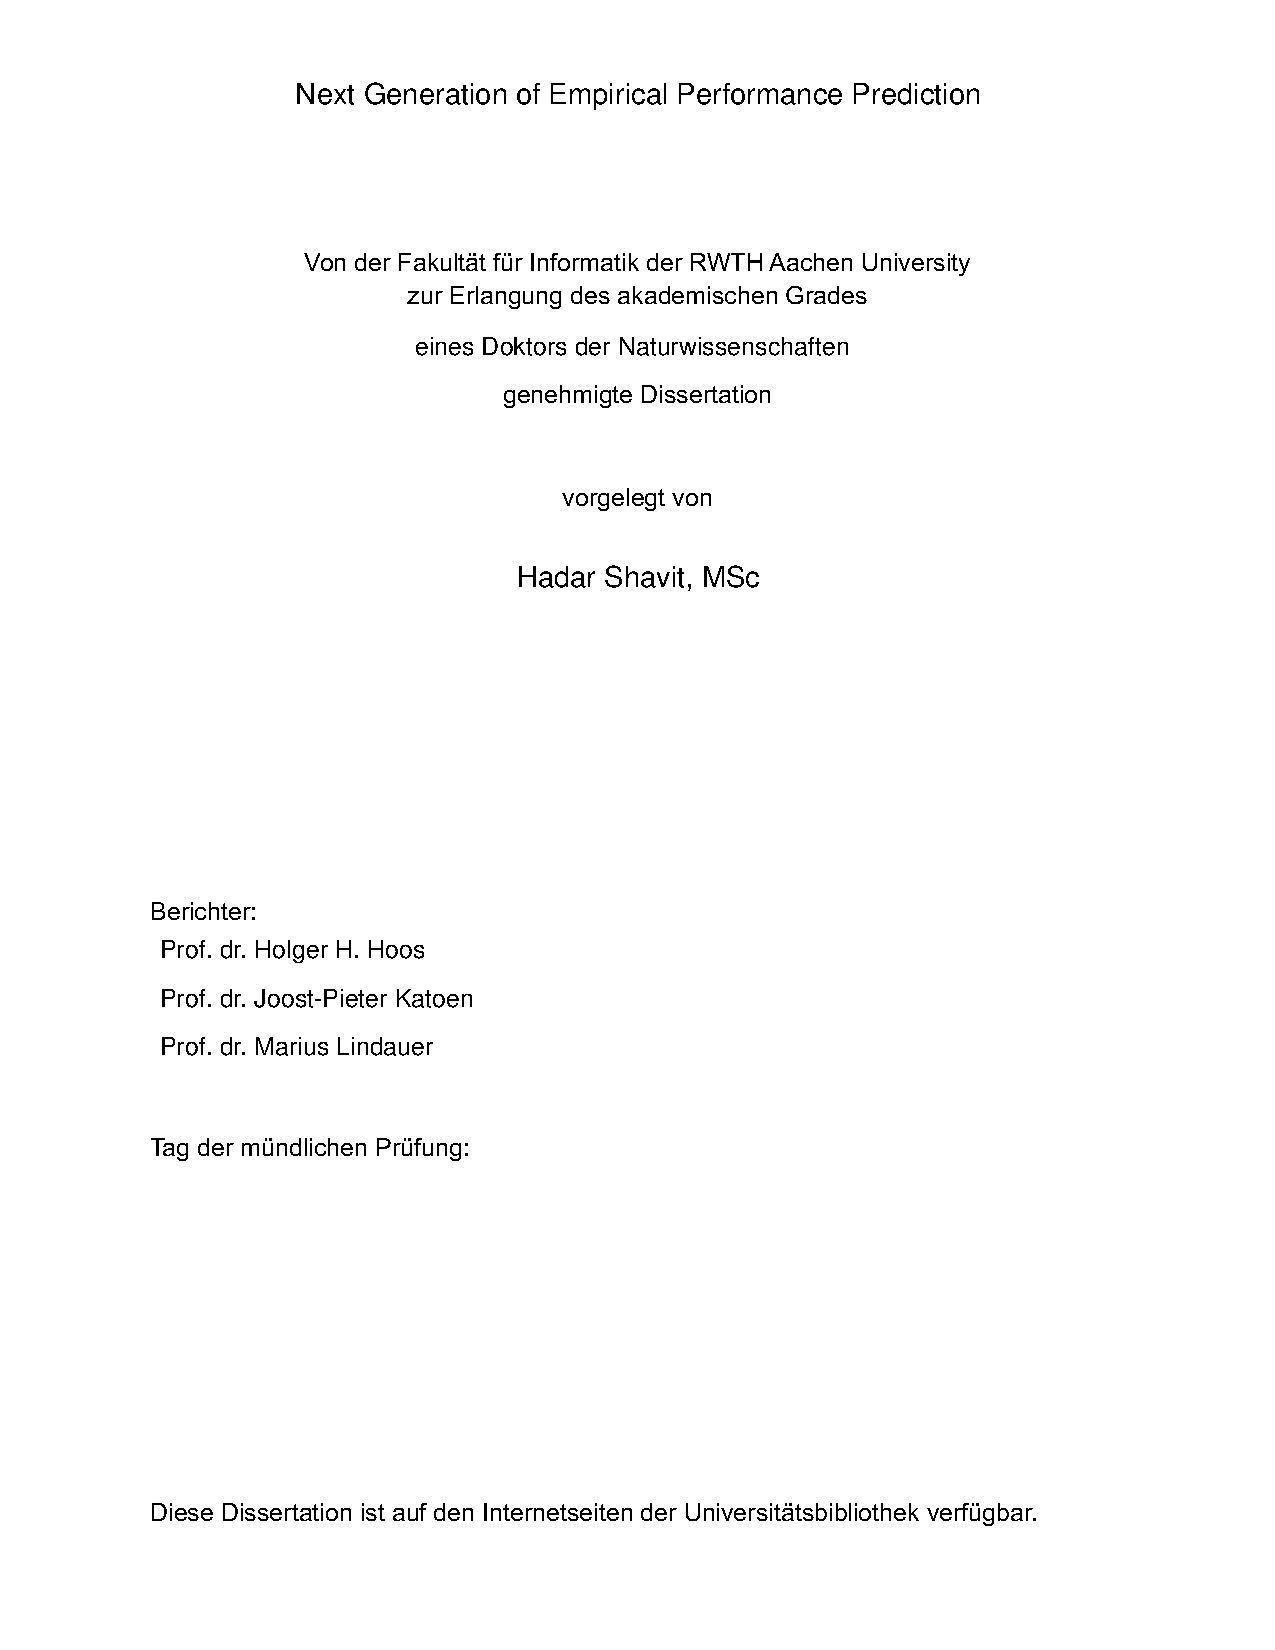
\includepdf[pages=1,fitpaper=true,pagecommand={\thispagestyle{empty}}]{FrontBackmatter/Deckblatt.pdf}

% \thispagestyle{empty}

\hfill

\vfill

\noindent\myName: \textit{\myTitle,} \mySubtitle, %\myDegree, 
\textcopyright\ \myTime

%\bigskip
%
%\noindent\spacedlowsmallcaps{Supervisors}: \\
%\myProf \\
%\myOtherProf \\ 
%\mySupervisor
%
%\medskip
%
%\noindent\spacedlowsmallcaps{Location}: \\
%\myLocation
%
%\medskip
%
%\noindent\spacedlowsmallcaps{Time Frame}: \\
%\myTime

%*******************************************************
% Dedication
%*******************************************************
\newgeometry{hcentering}
\thispagestyle{empty}
%\phantomsection 
\refstepcounter{dummy}
\pdfbookmark[1]{Dedication}{Dedication}

\vspace*{3cm}

\begin{center}
    =
\end{center}

\medskip

\begin{center}
   =
\end{center}

\clearpage
\restoregeometry
%\cleardoublepage\include{FrontBackmatter/Foreword}
\cleardoublepage%*******************************************************
% Abstract
%*******************************************************
%\renewcommand{\abstractname}{Abstract}
\pdfbookmark[1]{Abstract}{Abstract}
\begingroup
\let\clearpage\relax
\let\cleardoublepage\relax
\let\cleardoublepage\relax

\chapter*{Abstract}


\vfill

\begin{otherlanguage}{ngerman}
\pdfbookmark[1]{Zusammenfassung}{Zusammenfassung}
\chapter*{Zusammenfassung}
Kurze Zusammenfassung des Inhaltes in deutscher Sprache\dots 
\end{otherlanguage}

\endgroup			

\vfill
\cleardoublepage%*******************************************************
% Publications
%*******************************************************
\pdfbookmark[1]{Publications}{publications}
\chapter*{Publications}

%\noindent Put your publications from the thesis here. The packages \texttt{multibib} or \texttt{bibtopic} etc. can be used to handle multiple different bibliographies in your document.

\begin{refsection}
    \small
    \nocite{*} % is local to to the enclosing refsection
    \printbibliography[heading=none,keyword=thesis-publication]
\end{refsection}

\cleardoublepage%*******************************************************
% Acknowledgments
%*******************************************************
\pdfbookmark[1]{Acknowledgments}{acknowledgments}

\begin{flushright}{\slshape    
    We have seen that computer programming is an art, \\ 
    because it applies accumulated knowledge to the world, \\ 
    because it requires skill and ingenuity, and especially \\
    because it produces objects of beauty.} \\ \medskip
    --- \defcitealias{knuth:1974}{Donald E. Knuth}\citetalias{knuth:1974} \citep{knuth:1974}
\end{flushright}




\bigskip

\begingroup
\let\clearpage\relax
\let\cleardoublepage\relax
\let\cleardoublepage\relax
\chapter*{Acknowledgments}
This dissertation marks the end of my PhD journey, a journey that started long ago. Since I was a child, I have been fascinated by computers and their potential to solve complex problems. 
I always wanted to understand how they work and how to make them work better. This curiosity me to study programming and computer science since a young age.
When I was at 9th grade, I started attending high school computer science lessons, thaught by Tamir Moav and Miki TBF. They introduced me to the world of algorithms and programming, and I was liked. I spent countless hours learning and experimenting with different different programs and algorithms, and I was amazed by the power and elegance of computer science.

This led me to pursue a degree in computer science at the Open University of Israel, a place that allowed me to explore my interests and develop my skills, even at a young age. I was fortunate to have many inspiring professors and mentors who guided me along the way, and I am grateful for their support and encouragement.

After completing my undergraduate studies, I decided to go for a short trip to the industry in the world of software engineering. I worked as a software engineer for a year, and I learned a lot about the practical aspects of programming and software development. However, I realized that my true passion was in research and academia, and I decided to pursue a PhD in computer science. Nonetheless, I am grateful for the experience and the skills I gained during my time in the industry, as it helped me to become a better researcher and a more well-rounded computer scientist. For this, I would like to thank my colleagues and mentors in the industry, who taught me valuable lessons about teamwork, communication, and problem-solving. Specifically, I would like to thank my former colleagues Harel Fuchs, Shahar Lupu, Yossi Babayof and Zahi Abou.

Following my the quick stint in the industry, I moved to Leiden for my master's degree in computer science, where I was introduced to the world of research and academia. The program at LIACS greatly expanded my knowledge and skills in computer science, with a focus on research. I would like to thank the professors and PhD students who guided me, specifically, Jan van Rijn, Wojtek Kowalczyk, E
\endgroup




\pagestyle{scrheadings}
\cleardoublepage%*******************************************************
% Table of Contents
%*******************************************************
%\phantomsection
\refstepcounter{dummy}
\pdfbookmark[1]{\contentsname}{tableofcontents}
\setcounter{tocdepth}{2} % <-- 2 includes up to subsections in the ToC
\setcounter{secnumdepth}{3} % <-- 3 numbers up to subsubsections
\manualmark
\markboth{\spacedlowsmallcaps{\contentsname}}{\spacedlowsmallcaps{\contentsname}}
\tableofcontents 
\automark[section]{chapter}
\renewcommand{\chaptermark}[1]{\markboth{\spacedlowsmallcaps{#1}}{\spacedlowsmallcaps{#1}}}
\renewcommand{\sectionmark}[1]{\markright{\thesection\enspace\spacedlowsmallcaps{#1}}}
%*******************************************************
% List of Figures and of the Tables
%*******************************************************
\clearpage

\begingroup 
    \let\clearpage\relax
    \let\cleardoublepage\relax
    \let\cleardoublepage\relax
    %*******************************************************
    % List of Figures
    %*******************************************************    
    %\phantomsection 
    \refstepcounter{dummy}
    %\addcontentsline{toc}{chapter}{\listfigurename}
    \pdfbookmark[1]{\listfigurename}{lof}
    \listoffigures

    \vspace{8ex}

    %*******************************************************
    % List of Tables
    %*******************************************************
    %\phantomsection 
    \refstepcounter{dummy}
    %\addcontentsline{toc}{chapter}{\listtablename}
    \pdfbookmark[1]{\listtablename}{lot}
    \listoftables
        
    \vspace{8ex}
%   \newpage
    
    %*******************************************************
    % List of Listings
    %*******************************************************      
      %\phantomsection 
    \refstepcounter{dummy}
    %\addcontentsline{toc}{chapter}{\lstlistlistingname}
    \pdfbookmark[1]{\lstlistlistingname}{lol}
    \lstlistoflistings 

    \vspace{8ex}
\endgroup
       
    %*******************************************************
    % Acronyms
    %*******************************************************
    %\phantomsection 
    \refstepcounter{dummy}
    \pdfbookmark[1]{Acronyms}{acronyms}
    \markboth{\spacedlowsmallcaps{Acronyms}}{\spacedlowsmallcaps{Acronyms}}
    \chapter*{Acronyms}
    \begin{acronym}[AutoML]
        \acro{ai}[AI]{Artificial Intelligence}
        \acro{api}[API]{Application Programming Interface}
        \acro{as}[AS]{Algorithm Selection}
        \acro{asf}[ASF]{Algorithm Selection Framework}
        \acro{automl}[AutoML]{Automated Machine Learning}
        \acro{bbo}[BBO]{Black-Box Optimisation}
        \acro{bert}[BERT]{Bidirectional Encoder Representations from Transformers}
        \acro{bertft}[BERT-FT]{fine-tuned BERT}
        \acro{bo}[BO]{Bayesian Optimisation}
        \acro{cg}[CG]{Closed Gap}
        \acro{clg}[CG]{Clause Graph}
        \acro{ci}[CI]{Continuous Integration}
        \acro{clip}[CLIP]{Contrastive Language-Image Pre-training}
        \acro{cnf}[CNF]{Conjunctive Normal Form}
        \acro{dag}[DAG]{Directed Acyclic Graph}
        \acro{dpll}[DPLL]{Davis-Putnam-Logemann-Loveland}
        \acro{epm}[EPM]{Empirical Performance Model}
        \acro{gnn}[GNN]{Graph Neural Network}
        \acro{hpo}[HPO]{Hyperparameter Optimisation}
        \acro{ice}[ICE]{Individual Conditional Expectation}
        \acro{mit}[MIT]{Massachusetts Institute of Technology}
        \acro{mlp}[MLP]{Multi-Layer Perceptron}
        \acro{ood}[OOD]{Out-of-Distribution}
        \acro{par}[PAR]{Penalised Average Runtime}
        \acro{pddl}[PDDL]{Planning Domain Definition Language}
        \acro{pep8}[PEP 8]{Python Enhancement Proposal 8}
        \acro{rmse}[RMSE]{Root Mean Squared Error}
        \acro{saps}[SAPS]{Scaling and Parameter Search}
        \acro{sat}[SAT]{Propositional Satisfiability}
        \acro{sbs}[SBS]{Single Best Solver}
        \acro{vbs}[VBS]{Virtual Best Solver}
    \end{acronym}

%********************************************************************
% Mainmatter
%*******************************************************
\cleardoublepage\pagenumbering{arabic}
%\setcounter{page}{90}
% use \cleardoublepage here to avoid problems with pdfbookmark
\cleardoublepage
\part{Preliminaries}

\noindent
The preliminary part introduces the motivation, research questions, and technical background for the dissertation.
Chapter~\ref{ch:introduction} presents the central thesis argument and contributions, while Chapter~\ref{ch:background} introduces the algorithm selection and Bayesian optimisation concepts used throughout the remaining chapters.

%************************************************
\chapter{Introduction}\label{ch:introduction}
%************************************************

Artificial intelligence (AI) has made significant progress in recent decades, both in research and practice. The ability of AI methods to solve various problems across a growing number of domains has led to their wide adoption in a variety of applications.
For example, deep learning methods are now able to classify images and to process natural language in a way that could not be imagined a few years ago. 
However, AI is much more than deep learning and image processing.
AI can be used for automated reasoning, where problems are modeled as logical statements and decisions are made through deduction. Also, AI is used to esnure that sytems, such as software and harware systems are functioning correctly and do not have security vulnerabilties.
Additional problems include optimisation problems, where AI methods are used to find well-performing solutions for given problems.

A common ground for all of the problems is that many algorithms exist to solve each of them, and each has many (hyper)parameters that control their behaviour. 
Furthermore, there exists many problem instances, where each algorithm with each hyperparameter configuration can perform differently, which in many cases can depend on the run, as the algorithms are stochastic.

Empirical performance prediction predicts the performance of (AI) algorithms on unseen problem instances, configurations or combinations of both, without running them. Such methods have various use cases, such as:
\begin{itemize}
    \item Automated algorithm selection (AS): choosing the best algorithm for a given problem instance
    \item Automated algorithm configuration (AC): choosing the best parameters for a given algorithm and problem instance
    \item Explaining algorithm behaviour: understanding why an algorithm performs well or poorly on a given problem instance
\end{itemize}

There exists additional use-cases of empirical performance prediction, however, they are not used in this dissertation. The field of empirical performance prediction is important for the advancement of AI, as it enables the development of more efficient and effective AI methods.

However, despite the great success of such methods, they are not commonly used in practice, or even, by researchers in other sub-fields of AI. This is partly because using the methods is hard, the performance is not good enough.
In this dissertation, we look at emprical performance prediction from a number of viewpoints, and propose methods to overcome some of the current limitations.

\section{Challenges in the field}

\subsection{Features are hard to extract, expensive and not always available}

When applying empirical performance prediction across instances, for example in automated algorithm selection and configuration techniques, a crucial first step is representing problem instances using descriptive numerical features. However, extracting high-quality features in practice faces several severe challenges, such as speed, instances size, and availability. Early in the work, we realised that for the famous SAT problem, where empirical performance prediction has long been applied, there are numerous difficulties extracting such features. These result from the advancement of computing systems, higher capabilities of SAT solvers, and more generally, the ever increased sizes of problem instances. Therefore, a better feature extraction mechanism is required to allow better features, which will in turn allow better performance prediction.

Additionally, many real-world problems are high-dimensional, which can cause severe scalability and performance degradation, often referred to as the curse of dimensionality, where the volume of the search space grows exponentially, making data points extremely sparse and search landscapes highly intractable. In black-box optimisation, this means that locating optimal solutions requires significantly more function evaluations, which can be prohibitively expensive. To solve such problems, empirical performance prediction is used in model-based optimisation. Additionally, estimating the performance of algorithms on unseen problem instances can provide be then used for algorithm selection and explainability. One approach to alleviate the issue of high dimensionality is to use dimensionality reduction techniques to project the high-dimensional search space onto a lower-dimensional subspace. However, while many dimensionality reduction methods exist, most of them have been developed and evaluated for classical machine learning tasks like clustering and classification, and it is not always clear how they perform on optimisation problems. Optimisation landscapes possess distinct properties where preserving target values and navigating the geometry of the search space are critical, unlike standard unsupervised tasks that focus solely on preserving global data variance. Consequently, there is a strong performance complementarity among different reduction methods across tasks, sample sizes, and dimensionalities, necessitating a systematic, task-driven assessment to guide the choice of the reduction technique.

\subsection{Models are not accurate enough}

Even with informative features, the predictive models and surrogate models used in algorithm selection, configuration, and Bayesian optimizsation must achieve high accuracy to guide decisions effectively. Standard modeling approaches face significant hurdles related to representation, target distribution, and optimisation dynamics. Traditional tabular models rely heavily on hand-crafted features, which may fail to capture the underlying topology and global structural properties of complex instances, such as Boolean formulas or planning graphs. In addition, algorithmic performance, especially for randomized heuristic solvers, is inherently stochastic, resulting in noisy target variables that are difficult to model. Performance data is also frequently right-censored because solvers are terminated at a predefined cutoff time, meaning the true execution time for unsolved instances is unknown, and standard regression models struggle to handle this censoring without yielding biased predictions. In the context of Bayesian optimisation, different surrogate models, such as Gaussian processes and tree-based ensembles, exhibit complementary strengths depending on the search space properties. Statically choosing a single surrogate model or using a fixed ensemble throughout the optimisation run often yields suboptimal results, as the model's suitability changes during different phases of the search trajectory. 
Finally, in optimisation contexts, traditional machine learning metrics like global mean squared error do not necessarily correlate with optimisation success. A surrogate model does not need to be uniformly accurate across the entire search space, yet it is poorly understood where accuracy is most critical, whether geometric proximity to the optimum or objective value quality is what prevents the acquisition function from being misled into suboptimal regions.

\subsection{Hard to use existing methods and to gain insights}

Finally, even when features can be successfully extracted and models are sufficiently accurate, deploying these methods in practical workflows and extracting scientific insights from them remains exceptionally difficult due to usability and explainability barriers. The algorithm selection and configuration communities have historically developed domain-specific tools in isolation, leading to separate pipelines for SAT solving, automated planning, or hyperparameter optimization. The absence of a unified, problem-agnostic library with a standardized API makes it difficult to apply methods developed in one domain to another, leading to redundant implementations and hindering fair benchmarking and reproducibility. Another major challenge is that most standard performance models predict a single scalar statistic, such as the mean running time, treating algorithm performance as a deterministic outcome. This ignores the run-to-run variation of randomized algorithms, making such models unsuitable for risk-sensitive applications where variance, skewness, and tail risks are critical. While probabilistic distribution predictors can capture run-to-run variance, explaining their predictions is difficult. Standard explainability techniques, such as partial dependence plots or individual conditional expectation curves, are designed for scalar-valued targets and cannot be applied directly to parametric distribution outputs. Explaining the raw parameters of a distribution is mathematically uninterpretable, necessitating methods that decompose predictions into interpretable statistics, such as mean, variance, or skewness, and map them back to instance features.

\section{Contributions of this thesis}

\noindent\textcolor{webgreen}{Hadar Shavit} and Holger H. Hoos (2024). ``Revisiting SATzilla Features in 2024.'' In: \textit{Proceedings of the International Conference on Theory and Applications of Satisfiability Testing (SAT 2024)}, pages 27:1--27:26.

Here, we revisit and modernize the feature extraction tool of the widely adopted SATzilla algorithm selector, which had not been updated since 2012. We replace the outdated preprocessors and solvers with contemporary versions, resolve compilation and memory errors encountered with modern, larger SAT instances, and introduce a user-configurable feature computation timeout.
Specifically, our contributions are:
\begin{itemize}
    \item[(a)] updating and modernizing the SATzilla feature extraction pipeline with contemporary preprocessors and solvers,
    \item[(b)] resolving compilation and memory limitations to allow feature extraction on modern, large-scale SAT instances, and
    \item[(c)] demonstrating significant performance improvements on satisfiability prediction, runtime prediction, and automated algorithm selection downstream tasks.
\end{itemize}

\vspace{1.5em}
\noindent\textcolor{webgreen}{Hadar Shavit}, Anja Jankovic, Elena Raponi, Thomas B\"ack, and Holger H. Hoos (2025). ``Task-driven Assessment of Dimensionality Reduction Methods for Machine Learning and Black-Box Optimisation.'' \textit{Under revision}.

Here, we present a systematic, task-driven benchmarking of 16 linear and non-linear, supervised and unsupervised dimensionality reduction techniques across diverse machine learning and black-box optimization tasks. We assess how well these techniques project search spaces while preserving critical target and landscape geometries, rather than just data variance.
Specifically, our contributions are:
\begin{itemize}
    \item[(a)] providing a comprehensive benchmark of 16 dimensionality reduction methods on both classical machine learning and black-box optimization tasks,
    \item[(b)] demonstrating that traditional unsupervised methods which focus on data variance can perform poorly when optimization target values and geometry are critical, and
    \item[(c)] revealing a strong performance complementarity among reduction methods, highlighting the necessity of a task-driven selection process.
\end{itemize}

\vspace{1.5em}
\noindent\textcolor{webgreen}{Hadar Shavit}, Anja Jankovic, Elena Raponi, Thomas B\"ack, and Holger H. Hoos (2025). ``DyMBO: Dynamic Mixture of Surrogate Models for Hyperparameter Optimisation.'' \textit{Under review at the Journal of Machine Learning Research (JMLR)}.

Here, we introduce DyMBO, a plug-in ensembling strategy for Bayesian optimization that dynamically selects and weights heterogeneous surrogate models. DyMBO evaluates the predictive ranking quality of candidate surrogates at each step and updates their weights using a memory-aware exponential moving average of their ranking losses.
Specifically, our contributions are:
\begin{itemize}
    \item[(a)] proposing a dynamic ensembling approach that weights surrogate models based on their recent ranking performance rather than global error,
    \item[(b)] introducing a memory-aware exponential moving average formulation to smoothly transition weights during the optimization trajectory, and
    \item[(c)] showing that DyMBO dynamically adapts to different search phases and consistently outperforms traditional static surrogate and ensemble baselines.
\end{itemize}

\vspace{1.5em}
\noindent\textcolor{webgreen}{Hadar Shavit} and Holger H. Hoos (2025). ``Graph Neural Networks as Empirical Performance Models.'' \textit{Manuscript in preparation}.

Here, we explore the use of Graph Neural Networks (GNNs) as empirical performance models (EPMs) to predict solver runtimes and select algorithms directly from graph representations of SAT instances. We construct a large-scale benchmark and evaluate multiple GNN architectures against standard tabular models trained on hand-crafted SATzilla features.
Specifically, our contributions are:
\begin{itemize}
    \item[(a)] building a large-scale benchmark scenario for graph-based SAT algorithm selection, covering multiple graph representations and solver portfolios,
    \item[(b)] evaluating the capability of GNNs to learn representation features directly from the topological structure of Boolean formulas, and
    \item[(c)] showing that GNNs achieve competitive prediction and selection performance without requiring expensive hand-crafted features.
\end{itemize}

\vspace{1.5em}
\noindent\textcolor{webgreen}{Hadar Shavit} and Holger H. Hoos (2025). ``Understanding Surrogate Model Accuracy in Bayesian Optimisation.'' \textit{Under revision}.

Here, we study how surrogate model prediction accuracy affects the performance of Bayesian optimization by formulating a ``noisy oracle'' surrogate framework. By systematically controlling prediction noise across different regions of the search space, we isolate the impact of accuracy from other confounding factors.
Specifically, our contributions are:
\begin{itemize}
    \item[(a)] introducing the noisy oracle framework to systematically study the impact of localized surrogate model accuracy,
    \item[(b)] proving theoretically and empirically that value-based accuracy near promising regions is much more critical than distance-to-optimum accuracy, and
    \item[(c)] showing that standard surrogates like Gaussian processes and random forests naturally exhibit this beneficial value-based accuracy pattern.
\end{itemize}

\vspace{1.5em}
\noindent\textcolor{webgreen}{Hadar Shavit} and Holger H. Hoos (2025). ``Explaining Algorithm Performance Distributions Through Interpretable Statistics.'' \textit{Manuscript in preparation}.

Here, we present a framework to predict and explain full running time distributions of randomized algorithms, addressing the limitations of traditional EPMs that only predict mean execution times. We introduce a tree-based XGBoost model for parametric distribution regression and extend explainability techniques to distribution predictors.
Specifically, our contributions are:
\begin{itemize}
    \item[(a)] proposing a tree-based XGBoost approach for parametric distribution prediction that matches neural-network accuracy at a lower computational cost,
    \item[(b)] developing explainability measures by decomposing predicted distributions into interpretable summary statistics like mean, variance, skewness, and kurtosis, and
    \item[(c)] demonstrating empirically that different instance features govern the scale versus the shape of algorithm performance distributions.
\end{itemize}

\vspace{1.5em}
\noindent\textcolor{webgreen}{Hadar Shavit} and Holger H. Hoos (2025). ``ASF: A Library for Automated Algorithm Selection in Machine Learning and Artificial Intelligence.'' \textit{Manuscript in preparation}.

Here, we introduce the Algorithm Selection Framework (ASF), a unified, problem-agnostic Python library designed to build, benchmark, and deploy automated algorithm selection pipelines. ASF bridges the gap between isolated, domain-specific algorithm selectors by offering a standardized, modular API.
Specifically, our contributions are:
\begin{itemize}
    \item[(a)] designing and implementing the first unified, problem-agnostic Python library for algorithm selection pipelines,
    \item[(b)] providing modular components for pre-selection, pre-solving, feature processing, and automated pipeline configuration, and
    \item[(c)] validating the library's versatility through diverse case studies in black-box optimization, AutoML, and out-of-distribution generalization.
\end{itemize}


\chapter{Background}\label{ch:ch02:background}



\section{Algorithm selection}
\label{sec:ch02:algorithm_selection}

In this section, we introduce the algorithm selection problem and its components, including a formal definition, common baselines and use cases. We also relate it to multi-class classification and empirical performance prediction.

\subsection{Formal definition}
Given a set of problem instances $\mathcal{I}$ (which can be, for example, datasets), instance features $\mathcal{F}$, a set of algorithms $\mathcal{A}$ and a performance metric $m:\mathcal{A} \times \mathcal{I} \rightarrow \mathbb{R}$ (for example, predictive accuracy or running time), the algorithm selection problem~\citep{Rice76} seeks to find a selector $S:\mathcal{F}\rightarrow\mathcal{A}$ such that the performance of $S$ on the instances $\mathcal{I}$ is optimal according to $m$~\citep{KerEtAl19}. 

Extensions include the use of \textit{algorithm features}, which are combined with the instance features to predict the best algorithm for each problem instance. For simplicity, for the remainder of the section, we assume that the goal is to minimise $m$.
In algorithm selection, the ideal goal is to reach the performance of the virtual best solver (\gls{vbs}) (\emph{i.e.}, perfect selector). Furthermore, the selection must be better than the single best solver (\gls{sbs}) in order to make the use of algorithm selection worthwhile.



Further details are provided in~\cref{sec:ch10:add_background}.

\subsection{Algorithm selection pipelines}
\begin{figure}[]
    \centering
    \resizebox{\linewidth}{!}{
    \begin{tikzpicture}[>=stealth, font=\normalsize]

        \fill[gray!5, rounded corners=8pt] (-0.5, 0.0) rectangle (26.0, 7.5);
        \definecolor{pipelineblue}{RGB}{30, 80, 140}
        \definecolor{evalgreen}{RGB}{30, 100, 50}
        \tikzset{
            data/.style={draw=pipelineblue!80!black, thick, fill=pipelineblue, text=white, rounded corners=4pt, text width=3.0cm, minimum height=1.3cm, align=center},
            process/.style={draw=pipelineblue!80!black, thick, fill=pipelineblue, text=white, rounded corners=4pt, text width=3.0cm, minimum height=1.3cm, align=center},
            eval/.style={draw=evalgreen!80!black, thick, fill=evalgreen, text=white, rounded corners=4pt, text width=3.0cm, minimum height=1.3cm, align=center},
            inputset/.style={align=center, font=\normalsize, text=black},
            metric/.style={align=center, font=\normalsize, text=black},
            arrow/.style={->, thick, draw=black!70},
            line/.style={thick, draw=black!70}
        }
        

        \fill[pipelineblue!10, rounded corners=6pt] (14.1, 3.1) rectangle (21.9, 4.9);
        \draw[dashed, pipelineblue!50!black, thick, rounded corners=6pt] (14.1, 3.1) rectangle (21.9, 4.9);
        \node[text=pipelineblue!80!black, font=\bfseries\scriptsize, anchor=south east] at (21.7, 3.25) {Core ML Pipeline};
        

        \node[inputset] (feat_sets) at (1.5, 6.0) {Set of Feature Sets\\[-0.5ex]\textnormal{\footnotesize \{$\mathcal{F}_1$, \dots\}}};
        \node[inputset] (instances) at (1.5, 4.0) {Set of Problem Instances\\[-0.5ex]\textnormal{\footnotesize \{$I_1$, \dots\}}};
        \node[inputset] (algos) at (1.5, 2.0) {Set of Algorithms\\[-0.5ex]\textnormal{\footnotesize \{$A_1$, \dots\}}};


        \node[process] (preselector) at (4.5, 2.0) {\textbf{Pre-selector}};
        \node[inputset] (usage_algos) at (7.5, 2.0) {Usage Set\\[-0.5ex]of Algorithms};


        \node[data] (features) at (10.5, 6.0) {\textbf{Features}};
        \node[data] (perf_data) at (10.5, 4.0) {\textbf{Performance}\\\textbf{Data}};
        \node[data] (algo_feats) at (10.5, 2.0) {\textbf{Algorithm}\\\textbf{Features}};


        \node[process] (ml_task) at (16.0, 4.0) {\textbf{Machine Learning}\\\textbf{Task}};
        \node[process] (presolving) at (16.0, 5.5) {\textbf{Pre-solving}};
        \node[process] (selector) at (20.0, 4.0) {\textbf{Algorithm}\\\textbf{Selector}};
        \node[eval] (perf_selector) at (24.0, 4.0) {\textbf{Performance of}\\\textbf{Algorithm Selector}};


        \node[metric] (perf_meas) at (18.0, 2.0) {Performance Measure(s)\\\textnormal{\footnotesize \{Accuracy, Running time, \dots\}}};



        \node[font=\small, text=black, fill=gray!5] (feat_comp) at (6.5, 6.0) {Feature Computation};
        \draw[line] (feat_sets.east) -- (feat_comp.west);
        \draw[arrow] (feat_comp.east) -- (features.west);
        \draw[arrow] (instances.east) -| (feat_comp.south);


        \draw[arrow] (algos) -- (preselector);
        \draw[arrow] (preselector) -- (usage_algos);
        

        \draw[arrow] (instances) -- (perf_data);
        \draw[arrow] (usage_algos.east) |- (perf_data.south west);
        \draw[arrow] (usage_algos.east) -- (algo_feats.west);


        \draw[line] (features.east) -| (13.0, 4.0);
        \draw[line] (algo_feats.east) -| (13.0, 4.0);
        \draw[line] (perf_data.east) -- (13.0, 4.0);
        \draw[arrow] (13.0, 4.0) -- (ml_task.west);


        \draw[arrow] (ml_task) -- (selector);
        \draw[arrow] (selector) -- (perf_selector);
        \draw[arrow] (features.north) |- (20.0, 7.0) -- (selector.north);
        \draw[arrow] (perf_data.east) -| (13.8, 5.5) -- (presolving.west);
        \draw[arrow] (presolving.east) -| (selector.110);


        \draw[arrow] (perf_meas.east) -| (perf_selector.south);
        \draw[arrow] (perf_meas.west) -| (13.5, 3.5) -- (perf_data.east |- 0, 3.5);

    \end{tikzpicture}
    }
    \caption[Algorithm selection pipeline]{Algorithm selection pipeline. A portfolio of complementary algorithms can first be chosen by pre-selection. In running-time scenarios, a short pre-solving schedule may solve easy instances before feature computation or before invoking the learned selector. Instance features, optional algorithm features, and performance data are then used to train and evaluate the algorithm selector.

    }
    \label{fig:ch02:asf_pipeline}
\end{figure}

Algorithm selection methods are integrated into \textit{algorithm selection pipelines}, which include several components:
\begin{itemize}
    \item \textbf{Pre-selection:} A subset of algorithms is selected from a larger candidate set. In most real-world scenarios, only a few algorithms contribute substantially to \gls{vbs} performance, yet having many candidates to choose from makes accurate selection harder and increases the risk of poor predictions. Pre-selection constructs a small, complementary portfolio. A prominent method for pre-selection is greedy selection based on marginal contributions~\citep{XuEtAl08}, where algorithms are iteratively added to the portfolio if they yield the largest improvement to the \gls{vbs} performance.


    \item \textbf{Pre-solving schedules:} For problems where the metric of interest is running time (e.g., $\mathcal{NP}$-complete problem solving), it is beneficial to first run a short schedule (\emph{i.e.}, a sequence of solvers, each executed with a specific cut-off time) of solvers to solve easy instances quickly, thereby avoiding unnecessary feature computation. Such methods use, for example, a greedy method to decide which algorithms to run~\citep{XuEtAl08}, or use an optimisation problem to find the optimal pre-solving schedule~\citep{HooEtAl12,KadEtAl11}.

    \item \textbf{Algorithm selection:} An algorithm (or a schedule of algorithms) is selected based on the computed features. This step typically involves a machine learning model. For example, there can be models that predict the performance for each instance~\citep{XuEtAl08,OztEtAl22}, models that predict the ranking of the algorithms~\citep{XuEtAl12,KerEtAl18}, formulating the problem as a recommendation task~\citep{MisSeb17} and other approaches.

\end{itemize}
Additionally, for algorithm selection, there is a need for two additional, problem specific components:
\begin{itemize}
    \item \textbf{Feature computation:} Representative features of the problem instance are computed and used as input to the learned selector. These features can be hand-crafted or learned from the data. The choice of features is crucial for the performance of the algorithm selector. For example, the SATzilla features are well-known to be a good representation of \gls{sat} instances~\citep{HutEtAl14,ShaHoo24}, while for machine learning datasets, there exists many features, such as the basic descriptors of~\citet{OztEtAl22} to more complicated features, that include advanced statistics, such as the ones implemented in PyMFE~\citep{AlcEtAl20}.

    \item \textbf{Evaluation metric:} This is an important component of algorithm selection, as it is used to evaluate the performance of the algorithm selector. While there exist broadly applicable metrics such as the performance of the \gls{vbs} and \gls{sbs}, their definition depends on the specific problem.


    Therefore, a problem-specific evaluation metric must be chosen that represents the performance of the algorithm. This can be, for example, accuracy, precision, recall, F1-score, AUC, running time and more, depending on the use-case.
\end{itemize}
An overview of the algorithm selection pipeline is presented in~\cref{fig:ch02:asf_pipeline}.




\subsection{Algorithm selection versus multi-class classification}
A common mistake among newcomers to algorithm selection is to treat it as a standard multi-class classification problem.
Although an algorithm selector predicts one algorithm from a finite set and 

can therefore be seen as performing a multi-class prediction task, training it as an ordinary multi-class classifier can yield sub-par performance, because it discards the performance of the algorithms relative to each other.

To see why, consider an instance where the performance gap between the best and the second-best algorithm is small.
In that case, selecting the second-best algorithm is a reasonable error.
A plain multi-class classifier, however, treats this outcome as equally wrong as choosing an algorithm that performs very poorly on the instance.
As we show in our ASlib experiments (\cref{sec:ch10:aslib_appendix}), multi-class classifiers can indeed perform far below the other methods in practice.


\section{Bayesian optimisation}


In this section, we define the \gls{hpo} problem and describe the working mechanisms of the \gls{bo} framework. 
We also cover related work on dynamic design choices related to the components of \gls{bo}, as well as using ensembles in \gls{bo}.

\subsection{Hyperparameter optimisation} Let $\mathcal{A}$ be a learning algorithm with $n$ hyperparameters, $\Lambda_{i}$ the domain of the $i$-th hyperparameter, and $\mathbf{\Lambda} = \Lambda_{1} \times \Lambda_{2} \times \dots \Lambda_{n}$ the overall hyperparameter configuration space. 
We denote a hyperparameter configuration by $\mathbf{\lambda} \in \mathbf{\Lambda}$, and the algorithm $\mathcal{A}$ with its hyperparameters instantiated to $\mathbf{\lambda}$ by $\mathcal{A}_{\mathbf{\lambda}}$.
Given a dataset $D$, the objective of \gls{hpo} is to find a hyperparameter configuration $\mathbf{\lambda}^{*}$ that minimises the loss $\mathcal{L}$ of a model fitted by algorithm $\mathcal{A}$ with hyperparameters $\mathbf{\lambda}$ on training data ${D}_{train}$, and evaluated on validation data ${D}_{validate}$, for a given loss function $\mathcal{L}$, \emph{i.e.},
\begin{equation}
\label{eq:ch02:def-hpo}
\mathbf{\lambda}^{*} \in \argmin_{\mathbf{\lambda} \in \mathbf{\Lambda}} 
\mathcal{L}(\mathcal{A}_{\mathbf{\lambda}}, {D}_{train}, {D}_{validate}) = \argmin_{\mathbf{\lambda} \in \mathbf{\Lambda}} c(\mathbf{\lambda})
\end{equation}
Here, $c(\mathbf{\lambda})$ is a shorthand for the loss function when $\mathcal{A}_{\mathbf{\lambda}}$ and $D$ are fixed.
Note that $c(\mathbf{\lambda})$ is a black-box function, without a closed-form expression nor analytic gradient information.

\subsection{Bayesian optimisation} 
\label{sec:ch02:bac_bo}
Bayesian optimisation (\gls{bo})~\citep{Mockus12,Garnett23,Frazier18,Kushner62,Kushner64} is a family of surrogate-based algorithms for efficient global optimisation of black-box problems.
\changed{Typically,} \gls{bo} consists of three main modules: an \emph{initial design}, \emph{i.e.}, in \gls{hpo}, a set of hyperparameter configuration candidates $\boldsymbol{\lambda} = (\lambda^{(1)},\ldots, \lambda^{(r)})$ and their evaluations 
$c(\boldsymbol{\lambda}) = (c(\lambda^{(1)}),\ldots, c(\lambda^{(r)}))$; a \emph{surrogate model} (fitted to the 

observations) that returns an approximation $\hat{c}(\mathbf{\lambda})$ of the unknown loss function $c(\mathbf{\lambda})$ while capturing the uncertainty in the prediction $\hat{\sigma}(\mathbf{\lambda})$ on unobserved points in the search space; and an \emph{acquisition function}, which is optimised to suggest solution candidates to be evaluated next, usually balancing exploration and exploitation of the search space.
\changed{\gls{bo} then evaluates the most promising candidates.} 

To approximate the expensive objective function, \gls{bo} typically employs a Gaussian process (GP) model as the surrogate. The GP model defines a distribution over functions on the configuration space $c(\lambda)\sim\mathcal{GP}_c(\mu(\lambda),k(\lambda,\lambda'))$, where 
$\mu(\cdot)$ 
is a mean function and 
$k(\cdot,\cdot)$
is a covariance function. If we consider an observation model 
$y_i = c(\lambda^{(i)}) + \varepsilon_i$
with normally distributed noise, 
$\varepsilon_i\sim\mathcal{N}(0,\sigma^2_\varepsilon)$, 
the predicted value by the GP model at one unknown configuration 
$\lambda$ will also follow a normal distribution with mean 
$\mu(\lambda)=K_{\lambda,\boldsymbol{\lambda}}(K_{\boldsymbol{\lambda},\boldsymbol{\lambda}}+\sigma^2_\varepsilon I)^{-1}\boldsymbol{y}$ and variance $\sigma^2(\lambda)=k(\lambda,\lambda)-K_{\lambda,\boldsymbol{\lambda}}(K_{\boldsymbol{\lambda},\boldsymbol{\lambda}}+\sigma^2_\varepsilon I)^{-1} K_{\boldsymbol{\lambda},\lambda}$, 
where $\boldsymbol{y}=(y_1,\ldots,y_r)$ is the vector of observations, $K_{\boldsymbol{\lambda},\boldsymbol{\lambda}}=[k(\lambda^{(i)},\lambda^{(j)})]_{\lambda^{(i)},\lambda^{(j)}\in\boldsymbol{\lambda}}$ is the covariance matrix, and $K_{\lambda,\boldsymbol{\lambda}}=[k(\lambda^{(i)},\lambda)]_{\lambda^{(i)}\in\boldsymbol{\lambda}}$ is the correlation vector for all samples.

GPs as a surrogate model inherently provide both the mean and the variance vector.

However, GPs are not the only surrogate model used in \gls{bo}. Another common choice for a surrogate model are tree-based models, 
such as random forests (RFs). 
Tree-based models traditionally predict only the mean of the given data (\emph{e.g.}, in a regression setting). 
In this case, the variance is defined based on the variance of the predictions of the leaves~\citep{HutEtAl11}. 
With $t(\lambda)$ being the prediction of a tree $t \in T$, we calculate the mean $\mu(\lambda)$ and variance $\sigma(\lambda)$ for a set of trees $T$ as follows:

\begin{equation}
    \mu(\lambda)=\frac{1}{|T|} \cdot \sum_{t\in T} t(\lambda) \; ,
\end{equation}
\begin{equation}
    \sigma(\lambda)=\frac{1}{|T|} \cdot \sum_{t\in T} (t(\lambda) - \mu(\lambda))^2 \; .
\end{equation}





Alternatively, uncertainty can be estimated via quantile regression~\citep{KoeBas78}, using two separate models to predict the upper and lower quantile of the output distribution, and deriving variance from the spread between these quantiles.
We adopt this approach to estimate uncertainty for another tree-based model, gradient boosting (GB); this is done similarly to the implementation in the \textsc{scikit-optimize} package.\footnote{\url{https://github.com/scikit-optimize/scikit-optimize}}



\Gls{bo} proceeds iteratively until a termination criterion is met. In each iteration, it optimises the acquisition function
by repeatedly querying the surrogate model to generate a pool of solution candidates. It then evaluates the most high-potential solutions (\emph{i.e.}, the solutions that maximise the acquisition function) from this pool,
refines the surrogate model based on the new observations, and updates the optimum if the new point improves upon the true function value of the best observation so far.

Among the many variants of \gls{bo} from the literature, in this work, we focus on the state-of-the-art method for \gls{hpo} to empirically evaluate our ensembling method: HEBO~\citep{CowEtAl22}.
HEBO (Heteroscedastic and Evolutionary Bayesian optimisation) is a \gls{bo}-based optimiser with several advancements 
\changed{
targeting each of the core \gls{bo} modules described above.
For the surrogate model, HEBO uses GP with two key transformations: a power transformation applied to the output observations $\boldsymbol{y}$ and a Kumaraswamy transformation applied to the input configurations $\boldsymbol{\lambda}$; 

jointly, these address heteroscedasticity in the noise $\epsilon$ and non-stationarity in the covariance matrix $K_{\boldsymbol{\lambda},\boldsymbol{\lambda}}$.
\citet{CowEtAl22} showed that these transformations enhance the ability of GPs to accurately approximate the mapping between configurations and corresponding performances, which is crucial for \gls{hpo}.


For the acquisition function, rather than optimising a single criterion, HEBO samples new candidate configurations by maximising MACE~\citep{LyuEtAl18}, a multi-objective acquisition function that simultaneously considers expected improvement (EI)~\citep{Mockus75}, probability of improvement (PI)~\citep{Kushner64}, and upper confidence bound (UCB)~\citep{ForEtAl08}, providing a more robust balance between exploration and exploitation of the search space than any single acquisition function alone.

Additional details on HEBO can be found in~\cref{sec:imp_det}.
}





\section{Chapter conclusion}

\paragraph{Connection to the thesis}~
The concepts introduced in this chapter provide the common language for the remainder of the dissertation.
Algorithm selection motivates the need for informative instance representations and robust performance models, while Bayesian optimisation motivates the study of surrogate models and the role of accuracy in decision making.
The next part therefore starts with the first dependency of any empirical performance model: the features and representations on which it is trained.

% %************************************************
\chapter{Related Work}\label{ch:related_work}
%************************************************


\cleardoublepage

\part{Better Features}

\noindent
This part begins with the objects on which empirical performance models operate: the representations of instances, data sets, and search spaces.
The chapters show that predictive performance is constrained not only by the learning algorithm, but also by whether the relevant information is available in a form that can be computed, compared, and used reliably.
The part starts with modernising hand-crafted \gls{sat} features, then studies dimensionality reduction as a task-dependent representation problem, and finally considers how surrogate-model suitability itself can be represented dynamically during optimisation.

\chapter{Revisiting SATzilla Features in 2024}\label{ch:ch03:rev_SATzilla}

\section{Introduction}





The Boolean satisfiability problem (\gls{sat}) is an important problem in computer science from both theoretical and practical viewpoints.
Common usages of \gls{sat} include hardware and software verification, cryptography, and more. 

However, as \gls{sat} is $\mathcal{NP}$-complete, it takes substantial time and computing power to solve it, which becomes prohibitively expensive as formulas become larger.

In order to deepen our understanding of \gls{sat} itself and develop better \gls{sat} solvers, it is of crucial importance to be able to describe \gls{sat} instances via an informative set of features.



Some of the most widely adopted such features are the SATzilla features~\cite{NudEtAl04,HutEtAl14}. 

These are a fixed set of features that are calculated from the DIMACS \gls{cnf} representation of a \gls{sat} instance. The SATzilla features consist of multiple groups, ranging from basic syntactic features describing the formula, such as its number of variables and clauses, to more complicated features, such as probing features derived from short runs of \gls{sat} solvers. Another type of features are based on statistics of graph representations of a given formula.

The SATzilla features have been successfully used in various domains, such as empirical performance models (\glspl{epm}; also known as performance or running time prediction) and algorithm selection~\cite{XuEtAl08,XuEtAl12}, algorithm configuration~\cite{HutEtAl11}, and benchmark generation~\cite{LeyEtAl09}. 

The features are also used for caching in CDCL-based model counting solvers~\cite{RooEtAl21} and in a variety of \gls{sat} solvers that incorporate machine learning techniques~\cite{GuoEtAl23}
However, the SATzilla features in their latest version date back to 2012. 

Since then, the \gls{sat} community has undergone various changes.
Most notably, \gls{sat} instances that we typically encounter today have a larger number of variables and clauses, thus taking significantly more time and memory to preprocess. Currently, the existing SATzilla feature extraction tool is unable to compute many of these features because of time and memory limitations.


In this paper, we revisit the SATzilla features and introduce a new version of the feature extraction tool. First, we replace the underlying solvers and the preprocessor with their most up-to-date versions. We then fix compilation errors and other memory errors related to dealing with larger formulas. Finally, we allow the user to set the time limits for feature computation. 
We compare the performance of our new tool with the old one in two \gls{sat} competitions. We measure the running times and the number of extracted features to check for performance gains of our new tool. We then evaluate the extracted features on three downstream tasks: satisfiability prediction, performance prediction and algorithm selection. We show that our new tool yields an important advantage in performance compared to the old tool across all three tasks.

The rest of the paper is organised as follows. We give a historical overview of the development and applications of the SATzilla features in~\cref{sec:ch03:related-work}. We then introduce the technical definitions, as well as the standard methodological pipeline in~\cref{sec:ch03:SATzilla-features}, wrapping it up with the contributions of this study. The results are presented in~\cref{sec:ch03:experiments}, and conclusions drawn in~\cref{sec:ch03:conclusions}.

\section{Related work}
\label{sec:ch03:related-work}












The SATzilla features were first introduced by Nudelman~et~al.~\cite{NudEtAl04} to construct \glspl{epm}, \emph{i.e.}, machine learning models that predict the running time of various \gls{sat} solvers given the features representing \gls{sat} instances. The authors identified key features that contribute the most towards having a good \gls{epm} prediction.

Consequently, they used the \glspl{epm} as a basis for algorithm selection, in which the algorithm that is selected corresponds to the one with the lowest predicted running time. 

They leveraged the \textit{performance complementarity} phenomenon of \gls{sat} solvers, where no \gls{sat} solver dominates all others over all instances. 
Therefore, selecting the best solver for each instance results in substantially better performance compared to choosing any standalone solver for all instances.
The SATzilla features were also successfully used for the satisfiability prediction task for \gls{sat} instances from various distributions~\cite{DevOSu08}. 



Further developments in algorithm selection led to the 2007 version of the SATzilla algorithm selector~\cite{XuEtAl08}, which combined running time and satisfiability prediction with other improvements. It won multiple medals in the \gls{sat} competition. This shows that extracting features from \gls{sat} instances can also speed up the solving process, and not only help understanding \gls{sat}. A newer version of the SATzilla algorithm selector was introduced in 2012~\cite{XuEtAl12}, winning multiple awards as well. It used a random forest as a predictor, and introduced an ensemble of pairwise classifiers to establish a ranking of the solvers, instead of predicting the running times directly. Additional features were introduced thereafter, revealing further important information about \gls{sat} instances. 




Another common usage of the SATzilla features is (model-based) algorithm configuration. To this end, the hyperparameters of \gls{sat} solvers are optimised such that their performance is as good as possible on all instances. As running \gls{sat} solvers is computationally expensive, a surrogate model is employed; it takes as an input a configuration of hyperparameters and instance features and predicts the performance of the \gls{sat} solver using a given configuration on a given instance. The instance features boost the accuracy of the surrogate model. An example of that is SMAC~\cite{HutEtAl11}, which successfully used the SATzilla features to optimise the performance of a wide range of \gls{sat} solvers on various benchmarks.


Last but not least, feature-based \glspl{epm} are proven to be useful for benchmark generation~\cite{LeyEtAl09}. In this context, given a new instance, we compute the features, which is usually cheaper than running a \gls{sat} solver, and use the \gls{epm} to predict whether the instance is hard (or not) for the solvers at hand.






















\section{SATzilla features}
\label{sec:ch03:SATzilla-features}


The SATzilla features describe the \gls{sat} formula using various representations and statistics. We briefly introduce three graph representations of a \gls{sat} formula, as undirected graphs are a meaningful representation of \gls{sat}, maintaining the permutation invariance: a) variable graph: nodes are variables, an edge exists if variables appear in the same clause; b) clause graph: nodes are clauses, an edge exists when two clauses share a negated literal; and c) variable-clause graph: nodes are variables and clauses, an edge exists between a variable node and a clause node if the variable appears in the clause.



Feature computation starts with the \emph{preprocessing} of the formula. This step, performed before solving an instance, renders the formula more accessible for \gls{sat} solvers. This means that the features are also computed on the version of the formula that is close to the one seen by the solvers. We believe that all these aspects can be boosted by using a modern preprocessor.
Features are classically computed using the \textsc{SATElite} preprocessor. We instead use the SBVA preprocessor, suggested by the winning solver from the 2023 \gls{sat} Competition. SBVA is also able to terminate after a set cutoff time, allowing for partial preprocessing, while \textsc{SATElite} does not include this functionality.
The preprocessed formula can then be directly used by a \gls{sat} solver without additional preprocessing within the solver, which improves the performance of algorithm selection.







Following the preprocessing, the \emph{feature extraction} begins. There are ten feature groups that can be extracted. We note that we describe the feature groups according to their implementation in the SATzilla feature extraction tool, not according to their definitions from the corresponding paper~\cite{HutEtAl14}. We point out that all feature groups include the time required to compute the features in the group.


\noindent\textbf{Preliminary} features include the number of variables and clauses before/after preprocessing. The running time of this feature group includes the preprocessing time and the time required to read the formula. \changed{This group contains 7 features.}

\noindent\textbf{Basic} features are cheap features that provide a basic description of the formula. They consist of the variable-clause ratio, the ratio between positive and negative literals in each clause, the number of unary, binary and ternary clauses, as well as statistics on clause nodes in the variable-clause graph. \changed{This group contains 15 features.}

\noindent\textbf{KLB} are expensive features that include the node degree statistics of the variable nodes in the variable-clause graph, and the ratio of positive to negative occurrences of each variable. They also include measures for the proximity to Horn formula, such as the fraction of Horn clauses and statistics on the number of times each variable appears in a Horn clause. \changed{This group contains 21 features.}

\noindent\textbf{Clause graph} (\gls{clg}) features are expensive features that contain statistics on the degree of the nodes in the clause graph, as well as the clustering coefficient. \changed{This group contains 11 features.}

\noindent\textbf{Diameter} features contain information on the diameter of the variable graph, which is the shortest path between each pair of nodes in the graph. \changed{This group contains 6 features.}

\noindent\textbf{\gls{dpll} probing} (or unit propagation) features are computed by running the \gls{dpll} algorithm for various depths and measuring the number of unit propagations at each depth. \changed{This group contains 6 features.}

\noindent\textbf{Lobjois} features are an estimation of the size of the search space. They are computed by running the \gls{dpll} algorithm multiple times until a contradiction is found. Then, the average depth of the contradictions is the log-estimation of the search space. 

\changed{This group contains 3 features, which are all based on the work of Lobjois and Lema\^{\i}tre~\cite{LobLem98}.}

\noindent\textbf{Survey propagation} features are based on computing statistics on the following probabilities returned by the VARSAT \cite{HsuMcI09} solver: a probability of each variable to be assigned to True, to False, and to be unconstrained. \changed{This group contains 19 features.}

    
\noindent\textbf{Clause learning} (CL) features are based on running a CDCL solver (ZChaff rand~\cite{MahEtAl04} in the 2012 version, CadiCal~\cite{BieEtAl20} in our new version) for two seconds. We measure the number and length of learned clauses for every 1000 decisions, and compute the statistics of those values. \changed{This group contains 19 features.}

\noindent\textbf{Local search} (LS) features are obtained by running two local search solvers many times, each time up to 10000 steps, and computing statistics on those runs. In the 2012 version, the local search solvers are GSAT and \gls{saps}. We instead use GSAT and Sparrow 2011 in our new version. \changed{This group contains 24 features.}

\noindent\textbf{Linear programming} (LP) features are based on solving a relaxed version of the \gls{sat} formula, 

where $C_1\land C_2\land \dots \land C_N$ is a Boolean formula \changed{with $N$ \gls{cnf} clauses $C_1 \ldots C_N$ over Boolean variables $x_j$. We now consider linear programming variables $x_j$ and
solve the following linear programming problem:
Maximise
    $\sum_{i=1}^N \sum_{l\in C_i} v(l)$, 
where the value $v(l)$ of literal $l$ is defined as $v(x_j)=x_j$, $v(\neg x_j)=1-x_j$, 
    while keeping
    $\sum_{l\in C_i} v(l) \geq 0$ 
    for each $C_i$ and $0 \leq x_j \leq 1$ for each $x_j$. 
    This means that every variable has a value between 0 and 1, each clause has a value which is the sum of values of all literals, and the value of the formula is the sum of values of all clauses. The goal is to maximise the value of the formula, while keeping the value of every clause positive. Finally, statistics on the linear programming solution are extracted. In the new version, we upgrade the linear programming solver package, lp solve. This group contains 7 features.}



We note that the basic, KLB and clause graph features are computed sequentially, with each feature group being dependent on the successful computation of the previous groups; \emph{e.g.}, if the computation of the basic features fails, the KLB and clause graph features will not be computed at all.

Another change we applied to the feature extraction tool is allowing a more precise timeout setting. In the 2012 version, the time limits were hard-coded and set to high values (for example, 1200 seconds for preprocessing). This can cause many feature computations to simply terminate without computing any features at all. To this end, we adjust the code in the new version to allow the user to set the time limits through a command line argument.

\section{Experiments}
\label{sec:ch03:experiments}
We evaluate our new SATzilla feature extraction tool on the formulas stemming from two latest (2022 and 2023) \gls{sat} Competitions. We first look at the feature extraction times and then evaluate the features on three downstream tasks: satisfiability prediction, running time prediction, and algorithm selection.

To assess the advantage of using the new version of the extraction tool, we extract the features using both our new version and the 2012 version of the tool, with a time limit of 180 seconds per feature group. 

We use a cluster of 18 nodes, each equipped with 2 AMD EPYC 7543 32-core CPUs with 256 MB L3 cache. Each node also has 1TB of memory. The cluster is running on a Rocky Linux 9.4 operating system. We measure running times using the runsolver tool \cite{Roussel11c}.

\subsection{Feature computation time}
\label{sec:ch03:feature-computation-time}

\begin{figure*}[h]
    \caption[Percentage of computed features (2022 SAT Competition)]{Percentage of features computed by the old tool (SATzilla 2012; in red) and the new tool (SATzilla 2024; in blue) over the available time budget for each feature group on the 2022 \gls{sat} Competition. For most feature groups, the new tool extracts features from more instances than the old one.}
    \centering
    \begin{subfigure}[b]{0.24\textwidth}
        \centering
        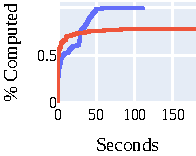
\includegraphics[]{figures/03/figs/ecdf_sc2022_Pre-featuretime.pdf}
        \caption{Preliminary}
        \label{fig:ch03:satcomp22_pre}
    \end{subfigure}
    \centering
    \begin{subfigure}[b]{0.24\textwidth}
        \centering
        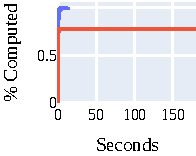
\includegraphics[]{figures/03/figs/ecdf_sc2022_Basic-featuretime.pdf}
        \caption{Basic}
        \label{fig:ch03:satcomp22_basic}
    \end{subfigure}
    \begin{subfigure}[b]{0.24\textwidth}
        \centering
        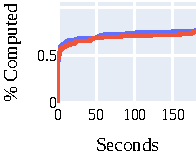
\includegraphics[]{figures/03/figs/ecdf_sc2022_KLB-featuretime.pdf}
        \caption{KLB}
        \label{fig:ch03:satcomp22_klb}
    \end{subfigure}
        \begin{subfigure}[b]{0.24\textwidth}
        \centering
        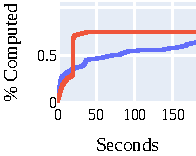
\includegraphics[]{figures/03/figs/ecdf_sc2022_CG-featuretime.pdf}
        \caption{Clause graph}
        \label{fig:ch03:satcomp22_cg}
    \end{subfigure}
    \centering
    \begin{subfigure}[b]{0.24\textwidth}
        \centering
        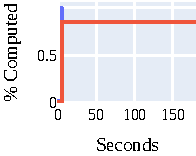
\includegraphics[]{figures/03/figs/ecdf_sc2022_cl-featuretime.pdf}
        \caption{Clause learning}
        \label{fig:ch03:satcomp22_cl}
    \end{subfigure}
    \begin{subfigure}[b]{0.24\textwidth}
        \centering
        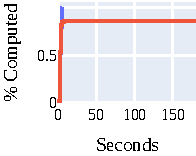
\includegraphics[]{figures/03/figs/ecdf_sc2022_ls-gsat-featuretime.pdf}
        \caption{LS: GSAT}
        \label{fig:ch03:satcomp22_ls_gsat}
    \end{subfigure}
        \begin{subfigure}[b]{0.24\textwidth}
        \centering
        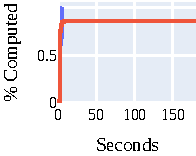
\includegraphics[]{figures/03/figs/ecdf_sc2022_ls-saps-featuretime.pdf}
        \caption{LS: \gls{saps}/Sparrow}
        \label{fig:ch03:satcomp22_ls_saps}
    \end{subfigure}
    \centering
    \begin{subfigure}[b]{0.24\textwidth}
        \centering
        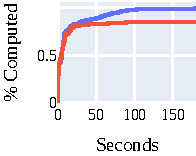
\includegraphics[]{figures/03/figs/ecdf_sc2022_sp-featuretime.pdf}
        \caption{Survey propagation}
        \label{fig:ch03:satcomp22_sp}
    \end{subfigure}
    \begin{subfigure}[b]{0.24\textwidth}
        \centering
        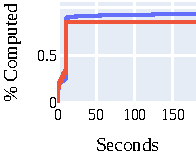
\includegraphics[]{figures/03/figs/ecdf_sc2022_DIAMETER-featuretime.pdf}
        \caption{Diameter}
        \label{fig:ch03:satcomp22_dia}
    \end{subfigure}
    \begin{subfigure}[b]{0.24\textwidth}
        \centering
        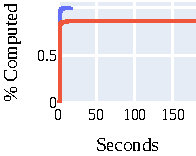
\includegraphics[]{figures/03/figs/ecdf_sc2022_lobjois-featuretime.pdf}
        \caption{Lobjois}
        \label{fig:ch03:satcomp22_lobjois}
    \end{subfigure}
    \begin{subfigure}[b]{0.24\textwidth}
        \centering
        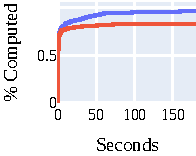
\includegraphics[]{figures/03/figs/ecdf_sc2022_unit-featuretime.pdf}
        \caption{Unit propagation}
        \label{fig:ch03:satcomp22_unit}
    \end{subfigure}
    \begin{subfigure}[b]{0.24\textwidth}
        \centering
        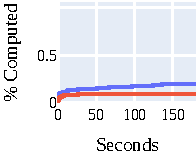
\includegraphics[]{figures/03/figs/ecdf_sc2022_lpTIME.pdf}
        \caption{Linear programming}
        \label{fig:ch03:satcomp22_lp}
    \end{subfigure}
    \label{fig:ch03:feat_comtimes_2022}
\end{figure*}

\begin{figure*}[h]
    \caption[Percentage of computed features (2023 SAT Competition)]{Percentage of features computed by the old tool (SATzilla 2012; in red) and the new tool (SATzilla 2024; in blue) over the available time budget for each feature group on the 2023 \gls{sat} Competition. For most feature groups, the new tool extracts features from more instances than the old one.}

    \begin{subfigure}[b]{0.24\textwidth}
        \centering
        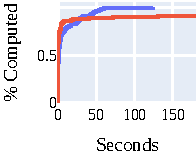
\includegraphics[]{figures/03/figs/ecdf_sc2023_Pre-featuretime.pdf}
        \caption{Preliminary}
        \label{fig:ch03:satcomp23_pre}
    \end{subfigure}
    \centering
    \begin{subfigure}[b]{0.24\textwidth}
        \centering
        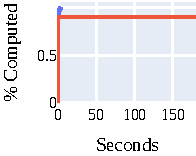
\includegraphics[]{figures/03/figs/ecdf_sc2023_Basic-featuretime.pdf}
        \caption{Basic}
        \label{fig:ch03:satcomp23_basic}
    \end{subfigure}
    \begin{subfigure}[b]{0.24\textwidth}
        \centering
        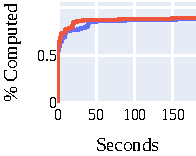
\includegraphics[]{figures/03/figs/ecdf_sc2023_KLB-featuretime.pdf}
        \caption{KLB}
        \label{fig:ch03:satcomp23_klb}
    \end{subfigure}
        \begin{subfigure}[b]{0.24\textwidth}
        \centering
        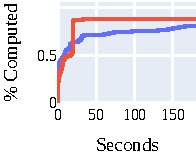
\includegraphics[]{figures/03/figs/ecdf_sc2023_CG-featuretime.pdf}
        \caption{Clause graph}
        \label{fig:ch03:satcomp23_cg}
    \end{subfigure}
    \centering
    \begin{subfigure}[b]{0.24\textwidth}
        \centering
        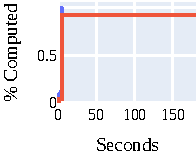
\includegraphics[]{figures/03/figs/ecdf_sc2023_cl-featuretime.pdf}
        \caption{Clause learning}
        \label{fig:ch03:satcomp23_cl}
    \end{subfigure}
    \begin{subfigure}[b]{0.24\textwidth}
        \centering
        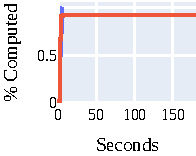
\includegraphics[]{figures/03/figs/ecdf_sc2023_ls-gsat-featuretime.pdf}
        \caption{LS: GSAT}
        \label{fig:ch03:satcomp23_ls_gsat}
    \end{subfigure}
        \begin{subfigure}[b]{0.24\textwidth}
        \centering
        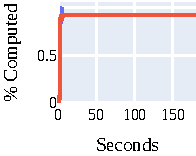
\includegraphics[]{figures/03/figs/ecdf_sc2023_ls-saps-featuretime.pdf}
        \caption{LS: \gls{saps}/Sparrow}
        \label{fig:ch03:satcomp23_ls_saps}
    \end{subfigure}
    \centering
    \begin{subfigure}[b]{0.24\textwidth}
        \centering
        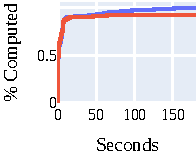
\includegraphics[]{figures/03/figs/ecdf_sc2023_sp-featuretime.pdf}
        \caption{Survey propagation}
        \label{fig:ch03:satcomp23_sp}
    \end{subfigure}
    \begin{subfigure}[b]{0.24\textwidth}
        \centering
        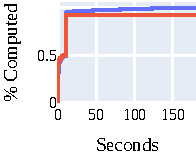
\includegraphics[]{figures/03/figs/ecdf_sc2023_DIAMETER-featuretime.pdf}
        \caption{Diameter}
        \label{fig:ch03:satcomp23_dia}
    \end{subfigure}
    \begin{subfigure}[b]{0.24\textwidth}
        \centering
        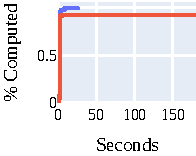
\includegraphics[]{figures/03/figs/ecdf_sc2023_lobjois-featuretime.pdf}
        \caption{Lobjois}
        \label{fig:ch03:satcomp23_lobjois}
    \end{subfigure}
    \begin{subfigure}[b]{0.24\textwidth}
        \centering
        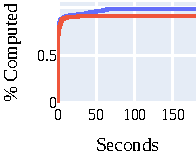
\includegraphics[]{figures/03/figs/ecdf_sc2023_unit-featuretime.pdf}
        \caption{Unit propagation}
        \label{fig:ch03:satcomp23_unit}
    \end{subfigure}
    \begin{subfigure}[b]{0.24\textwidth}
        \centering
        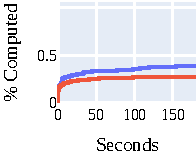
\includegraphics[]{figures/03/figs/ecdf_sc2023_lpTIME.pdf}
        \caption{Linear programming}
        \label{fig:ch03:satcomp23_lp}
    \end{subfigure}
    \label{fig:ch03:feat_comtimes_2023}
\end{figure*}

\cref{fig:ch03:feat_comtimes_2022,fig:ch03:feat_comtimes_2023} show the percentage of features computed over the available time budget using the old (depicted in red) and new (depicted in blue) SATzilla tool on the 2022 and 2023 \gls{sat} Competition data, respectively. For simplicity, due to the similarity of the overall results between the two competitions, we draw more detailed insights based on plots from the 2023 edition (\cref{fig:ch03:feat_comtimes_2023}). 

We first observe that the new tool is able to extract more features than the old one for most feature groups. In particular, we highlight the performance gains on the preliminary feature group (\cref{fig:ch03:satcomp23_pre}), for which the new tool can extract the features for all formulas, compared to less than $80\%$ of the formulas when using the the old tool. We note that for some feature groups, like graph learning (\cref{fig:ch03:satcomp23_cg}), the old tool is able to extract more features compared to the preliminary feature group. This is due to the fact that the old tool extracts the preliminary, basic, KLB and \gls{clg} feature groups together. Therefore, in case computing one of those groups takes a long time, the whole feature extraction fails.

We also note that for KLB and \gls{clg} features there is an advantage for the old version, due to the new SBVA preprocessing method yielding larger formulas than its predecessor \textsc{SATElite} (as in many cases smaller formulas are not always easier to solve). Similarly, the expensive graph-based features (\emph{e.g.}, \cref{fig:ch03:satcomp23_cg,fig:ch03:satcomp23_dia}) require more time to extract than smaller formulas. 

\changed{This is more apparent in the 2022 \gls{sat} Competition, where larger instances were used than in the 2023 \gls{sat} Competition.}




\subsection{Satisfiability prediction}
\label{sec:ch03:satisfiability-prediction}

The first downstream task is satisfiability prediction, for which we measure the performance when using features extracted by our tool. 

We use the random forest (RF) classifier from the scikit-learn package to learn the mapping between features (representing \gls{sat} instances) and outputs (satisfiable or unsatisfiable). We optimise the hyperparameters of the RF for one hour using SMAC3~\cite{LinEtAl22b} on 10-fold cross-validation of the training data.
We consider instances from the 2022 and 2023 \gls{sat} Competitions for which we know the satisfiability result (put differently, we omit instances for which the solution is unknown). On each competition, we evaluate the performance of the RF model using 10-fold cross-validation. This results in having outer cross-validation (for evaluation) and inner cross-validation (for training). Such techniques have been previously used by AutoFolio~\cite{LinEtAl15}.

We present the satisfiability prediction accuracy scores in \cref{fig:ch03:sat_prediction}. We see that, by using features extracted via the new tool, we achieve better performance across all instances on both \gls{sat} competitions. Furthermore, we notice that the new tool leads to a higher accuracy gain for satisfiable instances than for unsatisfiable instances. For the latter, the accuracy remains very similar to the one achieved by using the old tool in the 2023 \gls{sat} Competition and slightly dropped for the 2022 \gls{sat} Competition. This might be due to the fact that the unsatisfiable instances are larger on average, thus being more prone to timeouts even when using our new tool, \changed{which goes along with the worse performance in the 2022 \gls{sat} Competition, where the unsatisfiable instances were larger than in the 2023 \gls{sat} Competition}. We point out that such high accuracy was already achieved before for industrial \gls{sat} instances~\cite{DevOSu08}.


\begin{figure*}[h]
    \caption[Satisfiability prediction accuracy]{Accuracy of the satisfiability prediction task using a random forest with features extracted by the old (SATzilla 2012) and the new tool (SATzilla 2024). We see an overall higher accuracy for the new tool, which results from higher accuracy on satisfiable instances. On unsatisfiable ones, the accuracy remains the same.}
    \label{fig:ch03:sat_prediction}
    \begin{subfigure}[b]{0.49\textwidth}
        \centering
        

        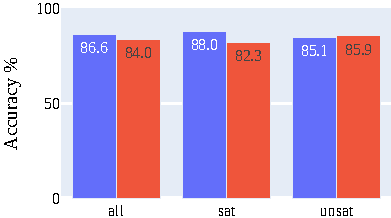
\includegraphics[]{figures/03/figs/sat_bar_2022.pdf}
        \caption{2022 \gls{sat} Competition}
        \label{fig:ch03:satpred22}
    \end{subfigure}
    \centering
    \begin{subfigure}[b]{0.49\textwidth}
        \centering
        

        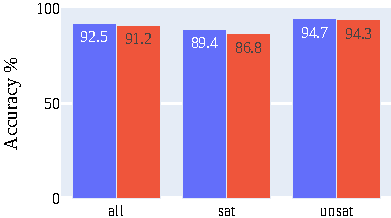
\includegraphics[]{figures/03/figs/sat_bar_2023.pdf}
        \caption{2023 \gls{sat} Competition}
        \label{fig:ch03:satpred23}
    \end{subfigure}
\end{figure*}


\subsection{Performance prediction}
The second downstream task we investigate is performance prediction, which has important applications in algorithm selection, configuration and benchmark generation. We refer to the methodology described in~\cite{HutEtAl14} and use a RF regressor as the \gls{epm}. It is important to note that for an accurate running time prediction we need to perform a $log_{10}$ transformation of running times prior to training the model, as done by Hutter 
\emph{et al.}~\cite{HutEtAl14}. This transformation allows to capture the order of magnitude rather than small variations in the running time. The \gls{epm} then maps instance features to the log-transformed running times, and we aim to minimise the root mean squared error (\gls{rmse}) of the model, which is defined as $\sqrt{\frac{1}{n}\cdot \sum_{i=1}^n (\hat{y}_i-y_i)^2}$ for $n$ predicted running times  $\hat{y}_i$ and ground truth running times  $y_i$. Lower \gls{rmse} scores are better and 0 is the optimal value.
In line with the previous task, we perform inner and outer cross-validation and optimise the RF's hyperparameters for one hour using SMAC3.

We look into the performance of the \gls{epm} for running time prediction on all solvers from the 2022 and 2023 \gls{sat} Competitions. Here, we do not actually run solvers on instances to record their running times, but rather use the running times reported by the competitions. We display the results for the 10 best solvers from each competition in \cref{fig:ch03:rt_pred} (the results for all solvers can be found in the supplementary material). We see that using the features extracted by the new tool leads to the lower \gls{rmse} for all solvers, compared to using those extracted by the old tool. For some solvers, we observe a significantly lower \gls{rmse}, like Kissat{\_}MAB{\_}prop-no{\_}sym, where using the new tool decreases the \gls{rmse} from 0.84 to 0.69. \cref{fig:ch03:rmse_hists} shows the histogram of the error percentage for all solvers in the 2022 and 2023 \gls{sat} Competitions. We see that for the 2022 competition, the new tool has more instances with error rate lower than $10\%$ compared to the old version. For the 2023 competition, using the features extracted with the new version, more instances are predicted with less than $1\%$ error. Histograms per solver are available in \cref{sec:rts_hists_per_solver}.

\begin{figure*}[h]
    \caption[RMSE of running time prediction]{Root mean square error (\gls{rmse}) of (log-transformed) running time prediction using a random forest with features extracted by the old (SATzilla 2012; in red) and the new tool (SATzilla 2024; in blue), on \gls{sat} solvers from the 2022 and 2023 \gls{sat} Competitions. The new tool achieves lower \gls{rmse} for all solvers.}
    \label{fig:ch03:rt_pred}
    \begin{subfigure}[b]{0.99\textwidth}
        \centering
        
        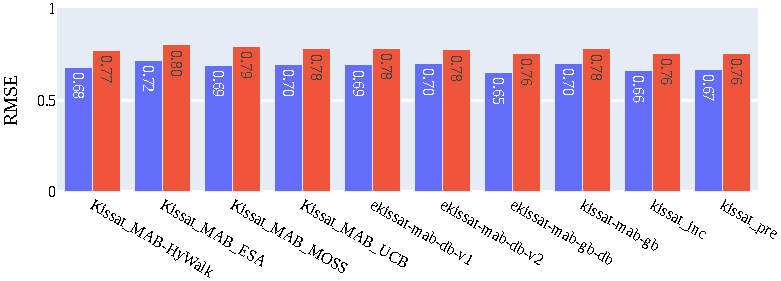
\includegraphics[]{figures/03/figs/rts_bar_2022.pdf}
        \caption{2022 \gls{sat} Competition}
        \label{fig:ch03:rt_pred22}
    \end{subfigure}
    \centering
    \begin{subfigure}[b]{0.99\textwidth}
        \centering
        
        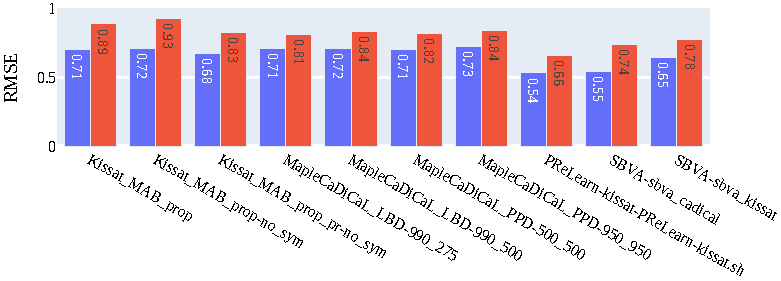
\includegraphics[]{figures/03/figs/rts_bar_2023.pdf}
        \caption{2023 \gls{sat} Competition}
        \label{fig:ch03:rt_pred23}
    \end{subfigure}
\end{figure*}


\begin{figure*}[h]
    \caption[Error percentage histogram of running time prediction]{Histogram of the error percentage of the root mean square error (\gls{rmse}) of (log-transformed) running time prediction using a random forest with features extracted by the old (SATzilla 2012; in red) and the new tool (SATzilla 2024; in blue), on \gls{sat} solvers from the 2022 and 2023 \gls{sat} Competitions. The new tool achieves lower error percentages.}
    \label{fig:ch03:rmse_hists}
    \begin{subfigure}[b]{0.49\textwidth}
        \centering
                

        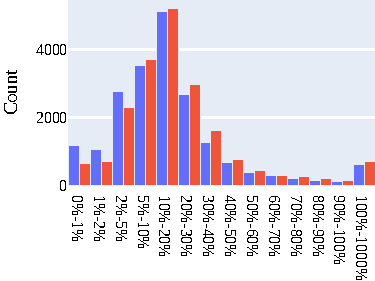
\includegraphics[]{figures/03/figs/acc_rt_pred_sc2022_both.pdf}
        \caption{2022 \gls{sat} Competition}
        \label{fig:ch03:rmse_hist_2022}
    \end{subfigure}
    \centering
    \begin{subfigure}[b]{0.49\textwidth}
        \centering
        

        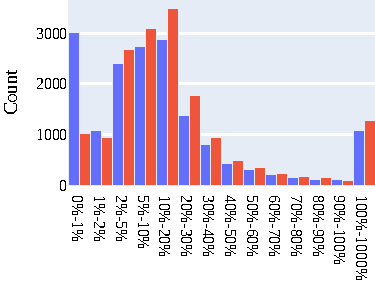
\includegraphics[]{figures/03/figs/acc_rt_pred_sc2023_both.pdf}
        \caption{2023 \gls{sat} Competition}
        \label{fig:ch03:rmse_hist_2023}
    \end{subfigure}
\end{figure*}

































\subsection{Algorithm selection}
The third and final downstream task we consider is algorithm selection. In algorithm selection, given a set of instances $I$, a set of solvers (\emph{i.e.}, algorithm portfolio) $\mathbf{A}$ and a performance metric $m: \mathbf{A} \times I \rightarrow \mathbb{R}$, we build an algorithm selector $S: I \rightarrow \mathbf{A}$ such that its performance is optimal on the instance set $I$ according to the metric $m$.
We compare the performance of algorithm selection to two standard baselines, the single best solver (\gls{sbs}; \emph{i.e}, the solver with the lowest overall running time) and the virtual best solver (\gls{vbs}; \emph{i.e.}, the theoretical oracle which for each instance selects the actual best solver on it).

We measure the performance of algorithm selection using \textit{closed gap}, which is computed as $\frac{m_{\gls{sbs}} - m_{S}}{m_{\gls{sbs}} - m_{\gls{vbs}}}$, (\emph{i.e.}, the closed gap stands for how much of the gap between the \gls{sbs} and the \gls{vbs} is closed by using the algorithm selector).
We then use AutoFolio~\cite{LinEtAl15} as an algorithm selector, which consists of multiple algorithm selection approaches, from which the best one is suggested by using algorithm configuration.


As algorithm portfolio for the selection, we use the 10 best solvers from each \gls{sat} competition. We train the selector for 8 hours.

\cref{fig:ch03:closed_gap} shows the closed gap results on the 2022 and 2023 \gls{sat} Competitions. Positive closed gap values on both scenarios using both the old and the new tool indicate that, in general, SATzilla features are useful for the algorithm selection task. 

Importantly, features extracted with the new tool lead to better closed gap values on both scenarios.

In \cref{fig:ch03:ecdf_as}, we provide ECDF plots showing the fraction of instances solved over time. In the 2022 \gls{sat} Competition scenario, the old version of the tool performs worse than the \gls{sbs} until a budget of approximately 1000 seconds, while the new version of the tool performs similarly to the \gls{sbs}. After 1000 seconds, both versions of the SATzilla features perform similarly. In the 2023 \gls{sat} Competition scenario, the new tool performs better than the old one for budgets between 100 and 1000 seconds. With a budget of less than 10 seconds, the old tool solves more instances. 

Overall, the ECDF plots reflect well what is shown in \cref{fig:ch03:closed_gap}, where we see that the new tool exhibits a few percents higher closed gap value.




\begin{figure}[h]
    \centering
    \caption[Closed gap values for algorithm selection]{Closed gap values for the algorithm selection task using the old (SATzilla 2012; in red) and the new tool (SATzilla 2024; in blue) on the 2022 and 2023 \gls{sat} Competitions; higher is better.}
    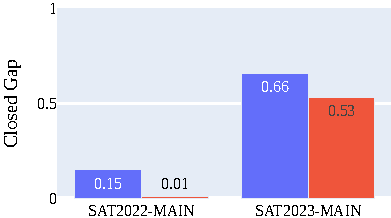
\includegraphics{figures/03/figs/as_bar_2023.pdf}
    \label{fig:ch03:closed_gap}
\end{figure}

\begin{figure*}[h]
    \caption[ECDF plots for algorithm selection]{ECDF plots for the algorithm selection task using the old (SATzilla 2012) and the new tool (SATzilla 2024) on the 2022 and 2023 \gls{sat} Competitions.}
    \label{fig:ch03:ecdf_as}
    \begin{subfigure}[b]{0.49\textwidth}
        \centering
        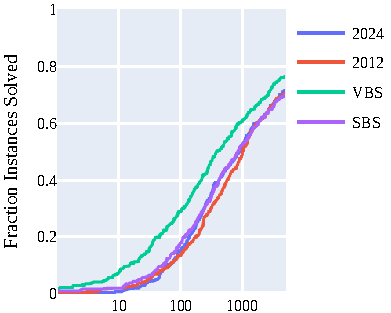
\includegraphics[]{figures/03/figs/ecds_af_2022.pdf}
        \caption{2022 \gls{sat} Competition}
        \label{fig:ch03:ecdf_as_2022}
    \end{subfigure}
    \centering
    \begin{subfigure}[b]{0.49\textwidth}
        \centering
        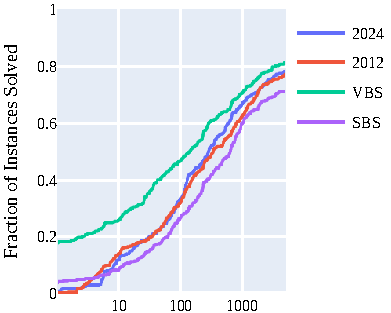
\includegraphics[]{figures/03/figs/ecds_af_2023.pdf}
        \caption{2023 \gls{sat} Competition}
        \label{fig:ch03:ecdf_as_2023}
    \end{subfigure}
\end{figure*}




































\section{Chapter conclusion}
\label{sec:ch03:conclusions}

This chapter introduced an improved version of the well-known SATzilla feature extraction tool, motivated by the need to make feature extraction more robust through better user infrastructure and bug fixes.
The new version uses up-to-date preprocessing techniques and \gls{sat} solvers, which allow for better representation of \gls{sat} formulae.
The experiments showed that the new tool improves satisfiability prediction, reduces error for running time prediction, and achieves a better closed gap for algorithm selection.

The SATzilla 2024 extraction tool aims to facilitate and promote the use of \gls{sat} features even beyond their current scope.
It is easily extensible and thus supports future work on new features, for example features based on recent developments in the explainability of \gls{sat} solvers~\cite{ElfEtAl18}, or other advancements in \gls{sat}.

\paragraph{Connection to the thesis}~
This chapter shows that empirical performance prediction can fail before modelling even begins if the underlying features are outdated, brittle, or too expensive to compute.
Modernising the SATzilla feature extractor therefore establishes the first thesis theme: better predictions require better access to reliable representations.
The next chapter broadens this representation question from \gls{sat} features to high-dimensional machine learning and black-box optimisation spaces.

\chapter{Task-driven Assessment of Dimensionality Reduction Methods for Machine Learning and Black-Box Optimisation}\label{ch:ch04:dim_red}

\section{Introduction}
\label{sec:ch04:intro}
High-dimensional data is ubiquitous in numerous application domains of machine learning and black-box optimisation.


In areas ranging from computer vision~\citep{SchEtAl15}, genome sequencing~\citep{VanEtAl22} and anomaly detection~\citep{TalEtAl21} to engineering~\citep{PreEtAl24}, hyperparameter optimisation~\citep{SehEtAl22} and neural architecture search~\citep{ElsEtAl19}, complex datasets with a large number of features defining 

a space to be searched for desirable design choices or solutions 
need to be handled effectively, in order to ensure that machine learning and  black-box optimisation algorithms applied to them are as accurate, efficient and scalable as possible. 
This poses a fundamental challenge in many applications, due to the curse of dimensionality, where the volume of the search space grows exponentially as data dimensionality increases, thereby degrading the performance of an algorithm applied to that data.
Data points become sparser in high dimensions, making it difficult for a machine learning algorithm to capture the underlying structure of the data and for a  black-box optimisation algorithm to locate good solutions for a given problem. 
At the same time, computational complexity severely increases, as well as the risk of overfitting in machine learning applications, leading to poor generalisation ability.

Dimensionality reduction methods serve as a crucial tool to address the challenge of manipulating high-dimensional data by evaluating the available information and extracting essential features from it.

The core principle of dimensionality reduction is to transform data from a high-dimensional space to a lower-dimensional one, revealing the underlying 

structure that is concealed in the original

data. 

Operating in a low-dimensional space enables machine learning algorithms to capture meaningful patterns in the data and  black-box optimisation algorithms to search for an optimal solution more effectively.
Traditionally, dimensionality reduction is used for machine learning tasks to reduce the input size of the data, as many machine learning algorithms (such as random forests~\citep{Breiman01} and support vector machines~\citep{CorVap95}) scale poorly with the number of features 

in terms of computational complexity. 
Dimensionality reduction methods are also employed for data clustering and visualisation~\citep{VanHin08}.
For classical applications, good performance of machine learning algorithms heavily relies on the ability of dimensionality reduction methods to preserve essential 

information contained in the data.
In the context of machine learning, this leads to higher interpretability of the models, reduced 

time and space complexity, less overfitting, and ultimately improved generalisation performance of machine learning models~\citep{JiaEtAl22}.

The curse of dimensionality is also a major obstacle for solving optimisation problems~\citep{Garnett23}. 

High-dimensional optimisation problems are widely encountered in the field of machine learning; for instance, the performance of machine learning algorithms crucially depends on the chosen values of the hyperparameters that govern their behaviour, and the performance of neural networks on some task of interest is heavily impacted by the choice of its architectural components~\cite{ElsEtAl19}.
Finding a well-performing set of hyperparameter values or a well-suited neural architecture for a given problem are  black-box optimisation problems, typically high-dimensional and expensive to evaluate.


Black-box optimisation algorithms used to tackle problems like these




do not have access to any information about the problem instance they aim to solve other than the evaluated samples from the search space. 

Typically, as the dimensionality of the search space increases, the volume grows exponentially, making it progressively more challenging for these algorithms to effectively locate good solutions. They also take more time to run in high-dimensional spaces.

In this context, dimensionality reduction methods have the potential to facilitate the optimisation process by transforming the high-dimensional problem landscape into a lower-dimensional one that may well be easier to tackle. 
We argue that preserving essential information about the data might not be imperative in the context of  black-box optimisation tasks (at least not in the way required for machine learning) if the performance of the optimisation algorithm is enhanced by navigating a more tractable landscape (assuming we are able to adequately reconstruct in the original space the points corresponding to the high-quality solutions 


in the reduced space).  

In recent years, there have been some attempts to leverage the power of dimensionality reduction for solving challenging optimisation problems in domains other than hyperparameter optimisation and neural architecture search~\citep{RapEtAl20,AntEtAl22,MeiWan21b,WanEtAl16b,KapEtAl16,AbbEtAl20}, where notably, the performance of (surrogate- and population-based) optimisation algorithms have been boosted by incorporating dimensionality reduction methods into the optimisation process.
Many real-world optimisation applications have high dimensionality, for example, in mechanical engineering~\citep{Jones08} and control problems~\citep{ZuoEtAl24}. 
Likewise, improving machine learning models in terms of scalability and accuracy by means of dimensionality reduction facilitates meta-learning and meta-optimisation approaches, such as algorithm selection and configuration, where state-of-the-art methods typically rely on predictions obtained from machine learning models, \emph{e.g.,} in the context of algorithm configuration~\citep{HutEtAl11}.




Most dimensionality reduction methods are traditionally developed and studied for classical machine learning use-cases.
How they perform in the context of  black-box optimisation is much less understood, despite the close link of the two fields via the existence of problems whose optimisation is crucial for the good performance of machine learning models.


Motivated by these ideas, we perform four complementary task-driven reduction benchmarking analyses, two in the context of machine learning and two in the context of  black-box optimisation, to better understand the strengths and weaknesses of dimensionality reduction methods in these scenarios.
We consider the following tasks:
(1) data clustering (unsupervised machine learning task), (2) classification of tabular data (supervised machine learning task), 
(3) regression for black-box function approximation (using a surrogate model trained on sampled data), 
and (4) a black-box optimisation procedure. 







\textbf{Our contribution:} We conduct a comprehensive benchmarking study on the effectiveness of various dimensionality reduction methods across two machine learning and two black-box optimisation tasks:\\






    \textbf{[Machine learning task 1]} 

    Cluster preservation by assessing the clustering ability in the reduced space, \emph{i.e.,} structural preservation of the data;
    we use hierarchical density-based clustering, which allows for the creation of clusters of varying densities and is 

    robust to parameter selection.\\ 


    \textbf{[Machine learning task 2]} 

    Predictive accuracy of ML algorithms on classification tasks of tabular data in the reduced space, \emph{i.e.,} investigating the effect of reducing the dimensionality of the datasets on the predictive performance of tabular classification models. \\
    \textbf{[Black-box optimisation task 1]}
    Target function approximation via a surrogate model

    in the reduced space, specifically fitting and evaluating the accuracy of a single-target regression random forest model on given benchmark problems, \emph{i.e.,} we predict the function values from the sampled solution candidates for each problem after dimensionality reduction.\\
    \textbf{[Black-box optimisation task 2]} Evaluation of optimiser performance in terms of regret, \emph{i.e.,} distance to the optimum, in the reduced space; as a case study, we focus on a Bayesian optimisation algorithm~\citep{Mockus12,Garnett23}, wherein we carry out the most resource-intensive tasks in the lower-dimensional space.

    This includes Gaussian process regression model training and the definition and evaluation of the acquisition function to predict new solution candidates for subsequent evaluation.






We evaluate the 

efficacy of the dimensionality reduction methods on these tasks on a wide variety of synthetic and real-world benchmarks of varying dimensionality (going as high as several thousand dimensions)
We vary the number of initial samples on which the dimensionality reduction methods are trained, with a particular focus on low sample sizes, which is a common setting in sample-efficient black-box applications.
We also consider multiple target dimensionalities for the reduced space.



From our results, we observed overall considerable differences in the performance of the dimensionality reduction methods we studied across various tasks, initial sample sizes and dimensionalities (both original and reduced).
In particular, the results indicated that, while the benchmarked dimensionality reduction methods exhibit relatively similar performances for the classical machine learning tasks, this does not hold for black-box optimisation scenarios.
In the context of black-box optimisation, depending on the setting at hand, we observed strong performance complementarity between the dimensionality reduction methods, emphasising the need for a careful selection of the dimensionality reduction method with respect to its intended use.

Therefore, our analysis aims to provide insights into how these methods leverage their working mechanisms depending on the task at hand, highlighting the crucial need for a thorough understanding of the intended use of the reduced space before choosing the appropriate method.

The remainder of this paper is organised as follows: in \cref{sec:ch04:dim_red}, we give an overview of dimensionality reduction, position our study in the broader related work context, introduce the methods selected for benchmarking, and give details on the transformation scheme required for dimensionality reduction methods to operate in the context of optimisation.
In \cref{sec:ch04:tasks}, we outline our methodology and present the four tasks designed to assess the performance of dimensionality reduction methods.
In \cref{sec:ch04:exp_setup}, we introduce the benchmark problem suites used in our empirical investigation and provide details on the setup of the experiments.
We present our results in \cref{sec:ch04:res}, analyse the running times of dimensionality reduction methods in \cref{sec:ch04:rt}, critically discuss our findings in \cref{sec:ch04:disc}, and provide concluding remarks in \cref{sec:ch04:concl}.

\section{Dimensionality reduction}
\label{sec:ch04:dim_red}


This section provides the necessary background of the concept of dimensionality reduction, including related work, descriptions of methods selected for this study, and the transformation scheme used for the optimisation tasks.


\subsection{Definition}






    












        


















    





There are two main ways to perform dimensionality reduction, either via feature selection or via feature extraction methods. 
Feature selection involves choosing a subset of features relevant for model construction, while eliminating irrelevant, redundant, and noisy features \citep{TheBho24}.

The goal is to attain the best-performing subset of the original features without resorting to any data transformation.



Despite being the most straightforward way to reduce dimensionality,
a prerequisite for feature selection is that the data exhibits a lower intrinsic dimensionality, allowing for the removal of features with minimal information loss. 
For many problems, this is not the case, as numerous features demonstrate high correlation, and this necessitates that data undergoes some transformation before we can perform dimensionality reduction.

Feature extraction involves creating new features from the original ones, where the new features are essentially images of the old ones through either linear or non-linear mappings \citep{ElhEtAl24}. 
This process can enhance separability in the problem, making it possible to reduce dimensions with minimal information loss. 

A drawback of feature extraction is the loss of 

meaning in the problem domain, 
preventing direct evaluation of the target in the reduced space. 

However, in black-box optimisation, for instance, the lower-dimensional space may be used for secondary tasks, while solutions are still searched for in the original space. 
Certain feature extraction techniques 
also
enable a backward mapping to the original space, specifically on a lower-dimensional manifold within the search space, where solutions can be evaluated~\citep{RapEtAl20}.


We formally define feature extraction as a transformation from a high-dimensional to a lower-dimensional space.
The exact formulation differs, based on the type of task at hand (machine learning or black-box optimisation).
For machine learning tasks, let $f: \X \rightarrow \Y $ be a machine learning model that transforms objects from the data domain $\X$ to the set $\Y$ of target values. 
Let $\D$ be a dataset that the model learns on, defined in either $\X$ as $\D = \{ \mathbf{x}_1, \dots, \mathbf{x}_N \} = X$ for unsupervised tasks or in $\X \times \Y$ as $\D = \{ \langle\mathbf{x}_1,y_1\rangle, \dots, \langle\mathbf{x}_N,y_N\rangle \} = \langle X,Y \rangle$ for supervised tasks.
Given original dimensionality $D$ of the data domain $\X$ and target (reduced) dimensionality $k$, each feature extraction learns a mapping $\T : \X \rightarrow \X'$ projecting from the original space into a reduced space $\X'$ of lower dimensionality $k < D$.
For black-box optimisation tasks, let $f: \R^D \rightarrow \R$ be a real-valued function defined on a $D$-dimensional domain. Given an initial sample $X = (\mathbf{x}_1, \dots, \mathbf{x}_N)$
of $N$ points generated uniformly at random, where $\mathbf{x}_i = (x_1, \dots, x_D)$ is a point denoted by its coordinates in a $D$-dimensional domain,
and their evaluations $Y = ({y}_1, \dots, {y}_N)$,
with ${y}_i = f(\mathbf{x}_i)$, 
each feature extraction method learns a mapping $\T: \R^D \rightarrow \R^k$ projecting from the original space into a reduced space of lower dimensionality, $k<D$.























































In this work, we focus solely on feature extraction techniques, as they exhibit a larger degree of flexibility and are able to extract meaningful information from a wider range of problems with different levels of complexities.
Feature extraction techniques are themselves categorised into supervised and unsupervised methods, depending on the availability of data labels (output values).




In~\cref{tab:ch04:dimensionality reduction-methods}, we list a range of supervised and unsupervised dimensionality reduction methods considered in this work; all of them are based on feature extraction.


Our criteria for selecting these methods for our study are outlined in \cref{sec:ch04:dimensionality reduction-methods}.

























We evaluate the performance of the feature extraction methods on four tasks, each analysing a different aspect of the resulting mapping. 
The evaluation is based on performance measures appropriate for each task 
in the reduced space,
operating on the pairs $(\T(\mathbf{x}),y)$ for machine learning and $(\T(\mathbf{x}),f(\mathbf{x}))$ for optimisation.


\subsection{Related work}
\label{sec:ch04:rel-work}




Dimensionality reduction techniques have predominantly been developed and studied in the context of classical machine learning.~\citet{VanEtAl09} conducted a comparative review of twelve methods with a special focus on non-linear ones and measuring their performance by the quality of the resulting low-dimensional data representation via the generalisation errors of $k$-nearest neighbour classifiers trained on those low-dimensional representations.~\citet{SubEtAl24} evaluated the performance of PCA and feature selection methods available in scikit-learn in terms of accuracy, precision, time and memory costs on standard classification tasks.~\citet{EspEtAl21} provide a quantitative survey of a wide range of methods; however, they do not conduct any benchmarking on downstream tasks. Similarly,~\citet{RayEtAl21} and~\citet{JiaEtAl22} proposed review papers on the well-known dimensionality reduction methods, without performing in-depth empirical comparison.

In recent years, dimensionality reduction has been increasingly used in concrete application domains where machine learning is prevalent.
In biology and medical science, several studies on performance comparisons between different dimensionality reduction techniques have been conducted for different use-cases.~\citet{EckEtAl24} compared nine dimensionality reduction methods for drug sensitivity prediction (focusing mostly on feature selection methods).~\citet{CanEtAl21} also investigated nine methods for reducing dimensionality of joint multi-omics data for the study of cancer.~\citet{BhaCha25} assessed the performance of three methods for visualising biomolecular energy landscapes.~\citet{ArmEtAl22} looked into the performance of various methods for reducing dimensionality of microbiome data.
In image retrieval,~\citet{ZhuEtAl14} compared a set of feature extraction and feature selection methods for large-scale image retrieval.


Bayesian optimisation in high-dimensional spaces has also received considerable attention in recent years, with numerous methods proposed to address the curse of dimensionality. 
REMBO~\citep{WanEtAl16b} exploits the assumption that high-dimensional objective functions often have low effective dimensionality by optimising within random low-dimensional subspaces.
Linear embedding approaches such as ALEBO~\citep{LetEtAl20} learn low-dimensional representations of the search space through adaptive coordinate transformations. 
Trust-region methods like TuRBO~\citep{EriEtAl19b} decompose the optimisation problem into local subproblems that are easier to solve in high dimensions.
BAxUS~\citep{PapEtAl22} employs axially aligned subspaces to reduce dimensionality while maintaining interpretability, while BOIDS~\citep{NgoEtAl25} exploits additive structure in the objective function. 
Random projection methods such as RPM-\gls{bo}~\citep{NguTra24} leverage the Johnson-Lindenstrauss lemma to perform optimisation in randomly projected subspaces. 
While these methods demonstrate the effectiveness of dimensionality reduction in Bayesian optimisation contexts, they are typically designed as integrated systems where the dimensionality reduction method is tightly coupled with the optimisation procedure. 
In contrast, this work does not propose a new Bayesian optimisation variant, but rather provides a systematic assessment of how different dimensionality reduction methods (when applied as preprocessing or embedding techniques) affect the performance of a standard Bayesian optimisation algorithm for diverse optimisation problems.


To the best of our knowledge, no comprehensive benchmarking study exists that assesses and compares a wide range of inherently different dimensionality reduction methods simultaneously in the context of machine learning and black-box optimisation.
Here, we emphasise that black-box optimisation problems lie at the core of many successful machine learning applications, and have so far been mostly neglected in terms of understanding how reducing the dimensionality of those problems might assist the optimisation process. 
Along these lines,~\citet{RapEtAl25} showed that global sensitivity analysis, when used as a dimensionality reduction technique, might oversimplify the landscape of the optimisation problem at hand, which renders it poorly suitable for these purposes. 
At the same time, they emphasise the importance dimensionality reduction methods might have in the optimisation context.









\subsection{Methods assessed in this work}
\label{sec:ch04:dimensionality reduction-methods}


\begin{table*}
    \centering
    \caption[Dimensionality reduction methods assessed]{Dimensionality reduction methods assessed in this work. All methods are based on feature extraction.


    }
    \label{tab:ch04:dimensionality reduction-methods}
    \small{
    \begin{tabular}{cccc} 
        \toprule
         Method&  Citation&  Type \\ \midrule
         PLS Regression& \citet{DeeEtAl90} &Supervised \\
         PCA (Linear)& \citet{Pearson1901} &  Unsupervised\\ 
         PCA (Cosine)& \citet{SchEtAl97}  &  Unsupervised\\ 
         PCA (Poly)& \citet{SchEtAl97}  &  Unsupervised \\
         PCA (RBF)& \citet{SchEtAl97}  &  Unsupervised \\ 
         PCA (Sigmoid)& \citet{SchEtAl97}  &  Unsupervised \\ 
         Fast ICA& \citet{HyvOja00} &  Unsupervised \\ 

         LLE& \citet{RowSau00} &  Unsupervised \\

         Gaussian Random Projection& \citet{Achlioptas01} & Unsupervised\\
         Sparse Random Projection& \citet{Achlioptas01} & Unsupervised \\
         Bernoulli RBM& \citet{HinEtAl06} & Supervised\\
         Incremental PCA& \citet{RosEtAl08} &  Unsupervised \\ 
         Dictionary Learning& \citet{MaiEtAl09}& Unsupervised \\
         Truncated SVD& \citet{HalEtAl11} &  Unsupervised\\ 
         Factor Analysis& \citet{Barber12} & Unsupervised\\
         LoLP& \citet{VogEtAl21}& Supervised\\



         
         
         
         
         
         
         

         \bottomrule
    \end{tabular}
    }
    
\end{table*}

We assess the effectiveness of 16 different feature extraction methods, 

covering unsupervised and supervised as well as linear and non-linear methods.
We first outline the working mechanisms of these dimensionality reduction methods, an overview of which is given in~\cref{tab:ch04:dimensionality reduction-methods}.

\begin{itemize}
    \item \textbf{Partial least squares (PLS) regression}~\citep{DeeEtAl90} 

    is a supervised linear method that identifies latent variables (components) which maximise the covariance between the input data and the target variables.  PLS regression
    iteratively constructs components by finding linear combinations of input variables that have maximum covariance with the target. In each iteration, the variation already explained by previous components is removed, and the process continues until the desired number of components is reached. PLS components are designed to be predictive of the target variable and are thus directly interpretable, making PLS regression suitable when dimensionality reduction is intended for prediction (regression or classification) tasks. PLS regression operates directly on the original data matrices, and has a lower computational overhead than many other methods.
    \item \textbf{Principal component analysis with linear kernel (PCA Linear)}~\citep{Pearson1901} is an unsupervised linear method equivalent to standard PCA, where the linear kernel is defined as the dot product between data vectors. The kernel matrix captures the pairwise similarities between data points based on their linear relationships in the original space, \emph{i.e.,} the original space does not undergo any transformation. The eigenvectors of the kernel matrix correspond to the principal components in the original space, and the eigenvalues represent the explained variance along each component. Put differently, PCA seeks to find the directions of maximum variance in the data covariance matrix, assuming they correspond to the most informative dimensions. PCA is especially useful for structured, linear data, but in the default implementation comes with a substantive computational overhead due to computing and storing the full kernel matrix, making it hard to use for large datasets. 

    \item \textbf{Principal component analysis with cosine kernel (PCA Cosine)}~\citep{SchEtAl97} is a variant of kernel PCA that uses cosine instead of linear kernel in order to capture non-linear relationships in the data. The cosine kernel focuses on angular relationships between data vectors rather than their magnitudes. It measures cosine similarity based on vector orientation, with values ranging from identical directions, over orthogonality, to opposite directions. Vector magnitudes are only used to normalise the data, projecting all data points onto the unit hypersphere before computing similarities. The fact that PCA with cosine kernel preserves only angular variance of the data makes it particularly effective for high-dimensional data where directional patterns are more meaningful than absolute values. 

    \item \textbf{Principal component analysis with polynomial kernel (PCA Poly)}~\citep{SchEtAl97} is a variant of kernel PCA that captures non-linear polynomial relationships in the data by implicitly mapping the data to a higher-dimensional space where polynomial feature interactions become explicit. The polynomial kernel is a positive definite kernel that computes similarities based on polynomial relationships between all pairs of data points. The eigendecomposition of the kernel matrix yields the principal components in the polynomial feature space, which capture directions of maximum variance among the polynomial feature combinations. This enables PCA to find curved, non-linear principal components in the original space, making it suitable for data with inherent global polynomial structure. 

    \item \textbf{Principal component analysis with radial basis function kernel (PCA RBF)}~\citep{SchEtAl97} is a variant of kernel PCA that captures complex, non-linear relationships in the data by implicitly mapping the data to a higher-dimensional space where feature similarities are based on Euclidean distances. The RBF (also known as Gaussian) kernel is a positive definite kernel that measures similarity based on proximity in the original space. Unlike polynomial kernels that capture global algebraic relationships, RBF kernels focus on local patterns. The resulting principal components (obtained via the eigendecomposition of the kernel matrix) are non-linear functions of the original coordinates, able to follow curved paths through the data points; they capture the most significant non-linear variations in the data, assuming that they are smooth and continuous. This allows for the detection of complex, curved manifolds, spiral patterns and localised structures in the original space, and makes PCA with RBF kernel effective for datasets with inherent geometric structure. 
    \item \textbf{Principal component analysis with sigmoid kernel (PCA Sigmoid)}~\citep{SchEtAl97} is a variant of kernel PCA that employs a sigmoid (hyperbolic tangent) function to create a feature space which emphasises threshold-like relationships in the data. The sigmoid kernel computes similarities based on a tanh transformation of the linear dot product between data vectors, but it is not guaranteed to be positive definite at all times. The feature space mapping of the sigmoid kernel, unlike other kernel PCA methods, captures both positive and negative relationships between data points, and is not distance-based, thereby modelling transition regions rather than smooth polynomial curves. 
    The tanh transformation introduces non-linearity while maintaining sensitivity to both the magnitude and direction of the linear dot product. The eigendecomposition of the kernel matrix yields principal components in the sigmoid feature space, which capture decision boundary- and threshold-like structures in the original data. This makes PCA with sigmoid kernel particularly suitable for data where relationships involve step-like changes or sigmoid curve-shaped transitions between different data regions, states or classes.
    \item \textbf{Incremental principal component analysis (Incremental PCA)}~\citep{RosEtAl08} is a memory-efficient PCA variant that works similarly to PCA with linear kernel, but allows mini-batch processing, updating principal components as new data becomes available. The covariance matrix is updated incrementally using rank-one updates, and the corresponding eigendecomposition can be maintained without recomputing from scratch. Incremental PCA is suitable for evolving data distributions, data streams, and other non-stationary environments.

    \item \textbf{Fast incremental component analysis (Fast ICA)}~\citep{HyvOja00} is a linear method stemming from signal processing, where it is used to separate multivariate signals into statistically independent components. As a dimensionality reduction method, it identifies the most significant independent sources underlying observed data, assuming that observed data is a linear combination (or mixture) of unknown independent source signals. This fundamental assumption of statistical independence of components is stronger than the assumption of uncorrelatedness by PCA-based methods. Fast ICA seeks to maximise non-Gaussianity of the recovered components (thereby achieving independence), which are then most likely to correspond to individual sources. Maximising non-Gaussianity measures (such as kurtosis or negentropy) is done using a fixed-point iteration scheme. The most significant independent components are selected based on their contribution to total variance, their degree of non-Gaussianity, or other domain-specific criteria. They represent different types of underlying source patterns, unlike components in PCA which are ordered based on the explained variance. Fast ICA can reveal patterns that PCA might miss when the underlying sources do not correspond to maximum variance directions. Moreover, components extracted by Fast ICA are interpretable and often correspond to meaningful physical or semantic sources. Fast ICA is therefore good at separating components with different statistical characteristics, and is particularly well-suited for dimensionality reduction in cases where independent generating processes of the data are plausible.

    \item \textbf{Locally linear embeddings (LLE)}~\citep{RowSau00} are a non-linear method that preserves local relationships between data points by assuming that high-dimensional data lies on or near a smooth, low-dimensional manifold and expressing each point as a weighted sum of its nearest neighbours. It then computes a low-dimensional embedding by finding coordinates in the lower-dimensional space such that each point can be reconstructed from its neighbours using the same weights as in the high-dimensional space. This ensures that local geometries such as distances and angles are preserved without assuming a global linear mapping. LLE is invariant to rotations, translations, and uniform scaling of the input data, but assumes that the data lies on a single, connected manifold. LLE is particularly well-suited for high-dimensional data visualisation and exploratory data analysis.
    \item \textbf{Gaussian random projection}~\citep{Achlioptas01} is a simple and computationally efficient method that projects the data into a lower-dimensional space by multiplying each data vector by a randomly generated projection matrix, whose elements are drawn independently from a Gaussian distribution with $\mu=0$ and $\sigma=\frac{1}{k}$. Random projections leverage the Johnson-Lindenstrauss lemma, 

    which states that a set of points in a high-dimensional space can be embedded into a space of much lower dimensionality such that pairwise distances are preserved with high probability. 


    \item \textbf{Sparse random projection}~\citep{Achlioptas01} replaces the dense Gaussian projection matrix with a sparse matrix (containing mostly zeros), reducing computational and memory requirements of the method above. The elements of the projection matrix are drawn randomly according to the following distribution:
    \begin{equation*}
        d_i= \begin{cases}
            \sqrt{\frac{s}{k}} & \text{with probability } \frac{1}{2s}\\
            0           & \text{with probability } 1 - \frac{1}{s}\\
            \sqrt{\frac{s}{k}} & \text{with probability } \frac{1}{2s}
        \end{cases}
    \end{equation*}
    where $s=\frac{1}{\sqrt{D}}$. 
    \item \textbf{Bernoulli restricted Boltzmann machine (RBM)}~\citep{HinEtAl06} is a probabilistic, neural-network-based method that captures complex, non-linear relationships in binary data. It learns a probability distribution where the hidden layer of a neural network serves as a lower-dimensional representation, performing dimensionality reduction through unsupervised learning. Bernoulli RBM learns to extract features that best reconstruct the original data, similar to an autoencoder but with stochastic binary units. The existence of the latter  makes Bernoulli RBMs particularly suitable for discrete or binary data.
    \item \textbf{Dictionary learning}~\citep{MaiEtAl09} is a sparse linear representation-based method that performs a sparse encoding of the data using a dictionary $\mathbf{D}$ of size $D\times k$. The transformation happens by multiplying the input vector by the dictionary. The method optimises the dictionary to reconstruct the original data as accurately as possible, in addition to ensuring that the low-dimensional data is sparse using $l_1$ norm. Unlike orthogonal transforms, Dictionary Learning typically uses overcomplete dictionaries where the number of basis vectors in the dictionary exceeds the data dimensionality. The quality of reconstruction depends on how well the learned dictionary captures the essential patterns in the data.
    \item \textbf{Truncated singular value decomposition (SVD)}~\citep{HalEtAl11} is an SVD-based method that computes only the top $k$ singular values and their corresponding singular vectors, rather than the complete SVD decomposition. Similar to traditional PCA, the directions of maximum variance in the data are preserved. It provides the best possible low-rank approximation to the original data matrix, effectively reducing dimensionality while preserving significant features. It is also computationally efficient, as it works directly with the original data and avoids explicit covariance computation. Truncated SVD is suitable for cases where data matrices are naturally sparse.
    \item \textbf{Factor analysis (FA)}~\citep{Barber12} is a statistical method that reduces the dimensionality by preserving the common factors of the data. Each data point is assumed to be a linear transformation of the low-dimensional latent factors, with the addition of Gaussian noise. It uses SVD to perform maximum likelihood estimation of the transformation matrix. Unlike PCA, which focuses on variance preservation and treats all variance as meaningful, factor analysis specifically aims to identify underlying constructs that explain correlations in the data. Factor analysis excels in psychological and social science research, as it provides insight into data structures beyond mere dimensionality reduction, offering substantive interpretation of what the reduced dimensions represent.

    \item \textbf{Linear optimal low-rank projection (LoLP)}~\citep{VogEtAl21} is a recent supervised method that learns linear projections optimised for class separability. It is designed for high-dimensional scenarios with low initial sample sizes. LoLP leverages both first and second moments (mean and covariance) of the data, unlike methods like PCA which only use the second moment, and it incorporates class label information to guide the projection, again unlike PCA that operates in an unsupervised manner.


\end{itemize}










We selected a range of 16 dimensionality reduction methods from the literature with readily available open-source implementations. 
All are accessible via Python packages that require only CPU computation and are not overly compute-intensive to be applied repeatedly in the second black-box optimisation task, where dimensionality reduction is performed multiple times in every iteration.


A crucial criterion for choosing a method for the study was the possibility of transforming inputs into a lower-dimensional space independently of training the method itself, \emph{i.e.,} we selected only those methods for which the \texttt{transform} method was natively supported in the original implementation on top of the standard \texttt{fit\_transform}.
Consequently, we do not include t-SNE~\citep{VanHin08} nor DensMAP~\citep{NarEtAl21}, neither of which supports \texttt{transform}.
Furthermore, we do not consider methods such as ivis~\citep{SzuEtAl19} and UMAP~\citep{SaiEtAl21}, due to their prohibitively high computational cost in the task of optimiser performance evaluation.
Methods such as NMF~\citep{LeeSeu00} and LatentDA~\citep{BleEtAl03} were also excluded, as they do not support negative values in the data.
We do not consider linear discriminant analysis (LDA), because it does not work for the regression task.
Finally, we exclude autoencoder-based dimensionality reduction approaches, since they do not have out-of-the-box readily available implementation and operate on a considerably different scale in terms of compute time compared to the other methods considered in this study.











\subsection{Transforming unsupervised into supervised}
\label{sec:ch04:transform}



Considering the goal of evaluating the performance of dimensionality reduction methods on the two black-box optimisation tasks, we are required to operate in a supervised environment.


In optimisation tasks, the sampled points are typically spread across the search space without carrying intrinsic structure; because of that, unsupervised methods cannot directly learn a meaningful representation of the problem. It is therefore necessary to redistribute the points so that their positions reflect their quality in terms of objective value. This enables unsupervised methods to discover latent patterns that are informative about the objective landscape.
To redistribute points, we use a weighting scheme proposed by~\citet{RapEtAl20}, which rescales points in the search space based on their function values, enabling us to also benchmark unsupervised dimensionality reduction methods in a supervised context. 

For machine learning tasks, we do not apply the weighting scheme, as we deal with clustering and classification on standard machine learning datasets, where we do not require the information about the quality of a point to be incorporated into its location.




The weighting scheme by~\citet{RapEtAl20} works by redistributing the initial sample $S$ over the search space so that it takes into account the information on the objective function. 

Point coordinates are then rescaled in such a way that points with a poor function value are pushed towards the origin and have less impact during the training of the feature extraction mapping.
Let $\{r_i\}_{i=1}^N$ be the ranking of the points in $S$ according to their function values $y$. The weights are computed as $w_i = \ln{N} - \ln{r_i}, \forall i=1,\dots,N$ and then normalised to form the weight vector $W$. 

We rescale the original data $S$ by removing its sample mean, \emph{i.e.}, $\bar{S} = S - \mathbf{1}_N\mu$, where
$\mu$ is the centre of mass of the sample and $1_N$ is the unitary vector of size $N$.
We then adjust each point with the corresponding weight, namely, $S' = \bar{S}W$.
For each of the unsupervised feature extraction methods that we benchmark, the initial sample on which they are trained first undergoes the rescaling. This means that the mapping is first learned on $S'$, and then applied to the centred sample $\bar{S}$.


















\section{Assessment methodology}
\label{sec:ch04:tasks}
In this section, we introduce four different tasks to assess the effectiveness of dimensionality reduction methods: two for machine learning and two for black-box optimisation.

The tasks are specifically designed to benchmark different aspects of dimensionality reduction methods, offering complementary views into these two different use-cases.

























\subsection{Machine learning}
\subsubsection*{Machine learning task 1: Clustering ability.}
\label{sec:ch04:method-ml-task1}

In this task, we investigate how the different dimensionality reduction methods affect the clustering of the samples in datasets in the reduced space, \emph{i.e.}, the final performance of an unsupervised machine learning approach.
By being able to cluster the samples, we verify whether a dimensionality reduction method preserves 

key structural aspects of the data.


To do so, given a dataset $\mathcal{D}$ with a train-test split $\mathcal{D}_{\text{train}}$ and $\mathcal{D}_{\text{test}}$, we first train a dimensionality reduction method $\T: X \subseteq \mathbb{R}^D\rightarrow \mathbb{R}^k$ on the training set $\mathcal{D}_{\text{train}}$. 


We then transform the test set instances $\mathcal{D}_{\text{test}}$ to the lower dimension and cluster the samples in $\mathcal{D}_{\text{test}}$ based on the features in the reduced space using a clustering algorithm $C$.


We measure the quality of the clusters $C(\T(\mathcal{D}_{\text{test}}))$ using two well-established clustering metrics~\citep{RosHir07}: homogeneity (which measures whether each cluster contains samples from the same true class) and completeness (which checks that all samples which belong to the same true class are in the same cluster).




\subsubsection*{Machine learning task 2: Tabular classification accuracy.}
\label{sec:ch04:method-ml-task2}

In this task, we assess the effect of 

different dimensionality reduction methods on classification tasks on tabular datasets, \emph{i.e.,} on the final performance of a supervised machine learning approach.
By evaluating the effectiveness of the dimensionality reduction methods on supervised tasks, we check whether the dimensionality reduction methods preserve correlation between the features and the labels of the data.
To do so, we train a dimensionality reduction method $\T$ on the training set $\mathcal{D}_{\text{train}}$. We then train an machine learning model $M$ on the transformed training set $\T(\mathcal{D}_{\text{train}})$. Finally, we use the machine learning model to predict the labels of the data in the test set: $M(\T(\mathcal{D}_{\text{test}}))$.

We evaluate the performance of well-known classical machine learning algorithms (random forest, multi-layer perceptron and gradient boosting) for solving the classification tasks using inputs from the reduced space.
Performance is measured using standard metrics such as accuracy, balanced accuracy and F1 score. The last two metrics are robust against imbalanced datasets, as some datasets might have more samples in some classes than the other.

\subsection{Black-box optimisation}

\subsubsection*{Black-box optimisation task 1: Target function approximation.}
\label{sec:ch04:method-bbo-task2}

In this task, we assess whether dimensionality reduction methods are able to capture information about the input $\mathbf{x}$ of the black-box problem relevant for accurate prediction of its function value $y$ in a lower-dimensional manifold.

We argue that the ability of a dimensionality reduction method to retain meaningful information necessary for accurately predicting output from input facilitates optimisation-related tasks (such as algorithm selection and configuration) that rely on machine learning predictions; in fact, this permits us to perform our tasks in a reduced space, thereby naturally decreasing the complexity of the task. 
Furthermore, transforming to a lower-dimensional space often leads to additional performance gains in terms of predictive accuracy, as the function becomes easier to approximate via the machine learning model. 





To assess this, we employ an approach based on empirical performance models~\citep{HutEtAl14}. 
We train a separate single-target regression random forest model to predict function values $y$ given solution candidates in the lower-dimensional space $\T(X)$ per setting (\emph{i.e.,} per function, instance, dimension, and dimensionality reduction method), as commonly done in empirical performance model settings~\citep{HutEtAl14,ShaHoo24}.

We evaluate prediction accuracy using root mean squared error (\gls{rmse}) scores for all models 


to quantify information loss.



\subsubsection*{Black-box optimisation task 2: Optimiser performance.}
\label{sec:ch04:method-bbo-task3}
In this task, we assess how the optimisation process is affected by operating in the reduced space using a Bayesian optimisation algorithm.

Bayesian optimisation~\citep{Garnett23} 

is a sample-efficient global optimisation framework, particularly well-suited for expensive-to-evaluate tasks.


We argue that performance gains in terms of optimisation and in terms of predictive accuracy (investigated in  black-box optimisation task 1) do not always positively correlate with one another. 
In fact, the essential knowledge about the problem that enhances the optimisation process might very well be different from knowledge needed to boost the predictive power of machine learning algorithms.

To assess this, we first collect an initial dataset of points in the original space using a Sobol sequence.
We then use pre-learned feature mappings to transform the inputs to the reduced space. 


Here, we fit a Gaussian process regression model, and we use the predicted mean and variance to define the acquisition function, specifically the expected improvement (EI)~\citep{SobEtAl08}, in lower dimensionality.  
We optimise EI by generating samples in the original space using a genetic algorithm, as done in the state-of-the-art Bayesian optimisation-based optimiser HEBO~\citep{CowEtAl22}. 








Subsequently, we transform this sample to the reduced space $\T(\mathbf{x})$ and calculate $\text{EI}(\T(\mathbf{x})), \text{for } \mathbf{x} \in X$. 
We then take the point with the highest EI value $\mathbf{x} \in \arg\max(\text{EI}(\T(\mathbf{x})))$ and evaluate it in the original space. 

We augment our dataset of sampled points using the newly evaluated point and update the Gaussian process accordingly in the reduced space.







We iterate this process until a stopping criterion is met.



We measure the performance of Bayesian optimisation assisted by different dimensionality reduction methods in terms of its efficiency in finding optimal solutions within the given evaluation budget.

































































































\section{Setup of experiments}
\label{sec:ch04:exp_setup}





We outline the setup used for our experiments, with details on benchmark problems, concrete design choices and implementation details for the machine learning tasks in \cref{sec:ch04:ml_setup}, and for the  black-box optimisation tasks in \cref{sec:ch04:bbo_setup}.
We conducted our experiments on two computer clusters.
For the machine learning tasks, we use Kathleen cluster, in which each node has two AMD EPYC 7543 32-Core processors with 512MB of L3 cache and 1TB of RAM running Rocky Linux 9.
For the black-box optimisation tasks, we used the CLAIX-2023 cluster, in which each node is equipped with 2 Intel Xeon 8468 Sapphire CPUs, 210MB L3 cache and 256GB RAM, running Rocky Linux 8. The code to reproduce our experiments, including the analysis is available at our GitHub repository\footnote{\url{https://github.com/hadarshavit/bench_dim_red_submission_code}}.

For all benchmarks (\emph{i.e.,} machine learning and black-box optimisation), we consider four different target dimensionalities, $k \in \{ 5, 10, 20, 40\}$, except in cases where the original dimension 
$D$ exceeds some of these values, which we handled by further restricting the values of $k$.


For all dimensionality reduction methods, we use their default scikit-learn~\citep{PedEtAl11} implementations, with default values of the hyperparameters such as kernel bandwidths for kernel PCA variants, number of neighbours for LLE, and dictionary size and sparsity for dictionary learning.
For methods tailored to binary inputs such as Bernoulli RBM, we use ordinal encoding to adapt the method to real-valued tabular and continuous optimisation data.




\subsection{Machine learning experiments}
\label{sec:ch04:ml_setup}

\subsubsection*{Benchmarks}

We use the OpenML~CC-18~\citep{BisEtAl21} and the classification datasets from the \gls{automl} Benchmark~\citep{GijEtAl24}, 

a well-known dataset collection used for benchmarking tabular machine learning algorithms. The collection contains various tabular classification tasks from different domains, with different sizes, numbers of classes and other characteristics. 


Each dataset comes with a set of pre-defined splits for $10$-fold cross-validation.

We choose high-dimensional datasets with at least 20 features, as in most applications 20 is a cut-off dimension at which the problem becomes considered as high-dimensional. The number of features in the datasets of ranges up to $3072$.


For computational reasons, we use datasets with up to 20\,000 samples. 



For machine learning tasks 1 and 2, we train the dimensionality reduction methods on the training folds. 
We then evaluate on the test folds the clustering performance in machine learning task 1 and the classifier performance in machine learning task 2.








\subsubsection*{Machine learning task 1: Clustering ability.}

As a clustering algorithm, we use HDBSCAN~\citep{CamEtAl13}, a hierarchical density-based clustering algorithm that allows for creation of clusters of varying densities and is more robust to parameter selection than other clustering algorithms such as $k$-means~\citep{KanEtAl02} and DBSCAN~\citep{EstEtAl96}.

We use the default implementation and default hyperparameter values of HDBSCAN.
Moreover, we provide results for other clustering metrics such as AMI, ARI and V-measure in the repository.
Due to limited additional insight they bring, we do not discuss them in detail in this study.


\subsubsection*{Machine learning task 2: Tabular classification accuracy.}
We consider the following three classification algorithms that are traditionally used for tabular data~\citep{GriEtAl22}: random forest, gradient boosting and multi-layer perceptron (\gls{mlp}), all in their scikit-learn~\citep{PedEtAl11} implementations.

We optimise all classifiers using SMAC3~\citep{LinEtAl22b}, a popular hyperparameter optimiser, with a budget of 30 evaluations. We provide the configuration spaces in~\cref{app:cs}.









\subsection{Black-box optimisation experiments}
\label{sec:ch04:bbo_setup}





\subsubsection*{Synthetic benchmarks}

We consider the Black-Box Optimisation Benchmark (BBOB) noiseless problem collection from the COCO framework~\citep{HanEtAl21}, accessible via the IOHprofiler tool~\citep{DoeEtAl18,WanEtAl22,DeNEtAl24}.
BBOB is a widely used benchmarking suite for assessing the performance of black-box optimisers, designed to cover a range of representative problems that are 


widely used in scientific studies of  numerical  black-box optimisation; 
for this reason, it is a particularly appropriate choice for our use-case.
It is composed of 24 continuous, noiseless, single-objective and scalable test functions defined on $[-5,5]^D$, with known difficulty (\emph{e.g.,} nonseparability, ill-conditioning, different levels of multimodality, adequate or weak global structure, etc.). 
For each function, we can generate arbitrarily many different instances by applying transformations (typically translations and rotations) to both the search space and the objective space. 
The BBOB problems are categorised into the following five classes: separable functions (f1-f5), functions with low or moderate conditioning (f6-f9),
functions with high conditioning and unimodal structure (f10-f14), multimodal functions with appropriate global structure (f15-f19), and multimodal functions with weak global structure (f20-f24).


In this work, we focus on the first 31 instances of each BBOB problem 


in seven different original dimensionalities, $D \in \{ 20,40,60,120,240,500,1000 \}$.
On each instance, we use a different pseudo-random seed for the data sampling 

conducted in the context of 
training the dimensionality reduction methods.










Full documentation on the BBOB problem collection (with definitions, visualisations and practical considerations) is available in the technical report by~\citet{FinEtAl09}.

\subsubsection*{Real-world benchmarks}

We also consider the following real-world benchmarks with different domains and dimensionalities:
\begin{itemize}
    \item Rover trajectory planning ($100D$)~\citep{WanEtAl18} is an optimisation problem, where the goal is to find an optimal trajectory between two given points in a $2D$ environment. A trajectory is determined by fitting a B-spline to a set of points.
    \item Mujoco~\citep{ManEtAl18,TodEtAl12} is a physics simulation engine with different environments, and the goal is to optimise a linear policy for locomotion tasks. We consider the Swimmer ($16D$), Hopper ($33D$), Walker-2d ($102D$), Half-cheetah ($102D$), Ant ($882D$) and Humanoid ($6392D$) environments.
    \item SVM hyperparameter tuning ($388D$)~\citep{EriJan21} optimises the hyperparameters of a kernel support vector machine on a regression dataset, including 3 regularisation hyperparameters and 385 kernel length scale hyperparameters.
    \item LassoBench~\citep{SehEtAl22} is a hyperparameter optimisation benchmark dealing with the optimisation of the weights in Lasso regression~\cite{GasEtAl09}. The number of weights depends on the number of input features in the datasets. From LassoBench, we use two high-dimensional real-world problems: Lasso-DNA ($180D$) and Lasso-Leukemia ($7129D$), as well as four synthetic problems: simple ($60D$), medium ($100D$), high ($300D$), and hard ($1000D$).
    \item MOPTA08 ($124
    D$)~\citep{Jones08,EriJan21} is a large-scale multidisciplinary optimisation problem of vehicle design in a crash test simulation. The goal is to minimise the total mass of the vehicle.
\end{itemize}

For all black-box optimisation benchmarks (both synthetic and real-world), we consider four different initial sample sizes to train the dimensionality reduction methods, $N \in \{100,200,500,1000 \}$.

\subsubsection*{Black-box optimisation task 1: Target function approximation.}

To build the surrogate, we sample $\min\{50 \cdot D, 5000\}$ using Sobol sampling.
We employ a random forest regressor as a surrogate model, specifically using the scikit-learn implementation. 
We use log-transformation for the target values and optimise 

the hyperparameter settings of the random forest using SMAC3~\citep{LinEtAl22b}.
To aggregate the results, we use min-max normalisation per function.
\subsubsection*{Black-box optimisation task 2: Optimiser performance.}
We use BoTorch~\citep{BalEtAl19} for the implementation of the EI acquisition function and the Gaussian process surrogate model.

To optimise the acquisition function, we use a genetic algorithm, similarly to the one used as a baseline in HEBO~\citep{CowEtAl22}, with a population size of 100 and 100 generations (10\,000 samples in total).
As an initial design, we evaluate $30$ points sampled via a Sobol sequence.
We use a Gaussian process with RBF kernel and optimise it the L-LBFGS-B, as done by default in BoTorch.
The total Bayesian optimisation budget is set at $300$ evaluations including the initial design, \emph{i.e.,} we run the Bayesian optimisation loop for $270$ evaluations.
































\section{Results}
\label{sec:ch04:res}


We present and discuss selected results from our experiments in \cref{sec:ch04:res-ml} for the machine learning tasks and in \cref{sec:ch04:res-bbo} for the black-box optimisation tasks.
Full results across all different settings are provided in the code repository\footnote{\url{https://github.com/hadarshavit/bench_dim_red_submission_code}}.



\subsection{Machine learning tasks}
\label{sec:ch04:res-ml}



\subsubsection*{Machine learning task 1: Clustering ability}


For the unsupervised machine learning task (\emph{i.e.,} clustering), we look at the results aggregated over all datasets for the two metrics (homogeneity and completeness) with different target dimensionalities $k$ in~\cref{fig:ch04:cluster_all_agg}. 
Regarding the cluster homogeneity metric, we first observe only small differences between the different target dimensionalities.
Most methods are unable to preserve cluster homogeneity, as the corresponding values of this metric are mostly below $0.3$.
This means that the data points within any one cluster created in the reduced space often do not have the same label as other members of the same cluster.
LLE, PCA (RBF) and PCA (Cosine) exhibit a slight performance edge over other methods according to this metric.
In rare cases, we observe outliers, whose presence indicates that, likely on specific datasets, these methods, as well as \emph{e.g.,} LoLP, are able to produce clusters with higher internal similarity of their members, \emph{i.e.,} the higher number of cluster members with the same label.

The relatively good results of LLE can be explained by the fact that


it preserves local neighbourhoods; therefore, classes that are locally separated in the original space are maintained by LLE better than by other methods.

These results show that dimensionality reduction methods do not preserve class clusters boundaries, therefore elements from several classes end up in the same cluster.


Regarding the cluster completeness metric, for low target dimensionalities, most methods achieve similar performance, while Gaussian and sparse random projections have the worst performance. 
However, in the case of higher target dimensionality, Gaussian and sparse random projections work very well. 
This can be explained by the Johnson–Lindenstrauss effect, which means that random projection preserves pairwise distances, 


thereby retaining the same assignment of elements to clusters both in the original and in the target dimensionality.






\begin{figure}
\centering
    \begin{subfigure}{0.24\textwidth}
        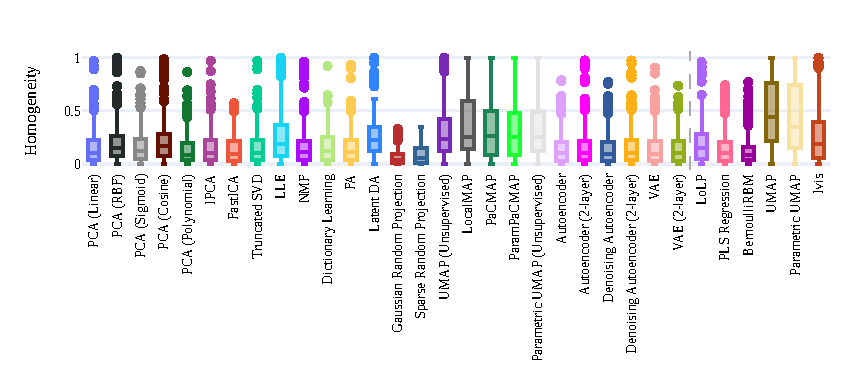
\includegraphics[width=\textwidth]{figures/04/ml/agg_5_homogeneity.pdf}
        \caption{\footnotesize{$k = 5$; homogeneity}}
    \end{subfigure}
    \begin{subfigure}{0.24\textwidth}
        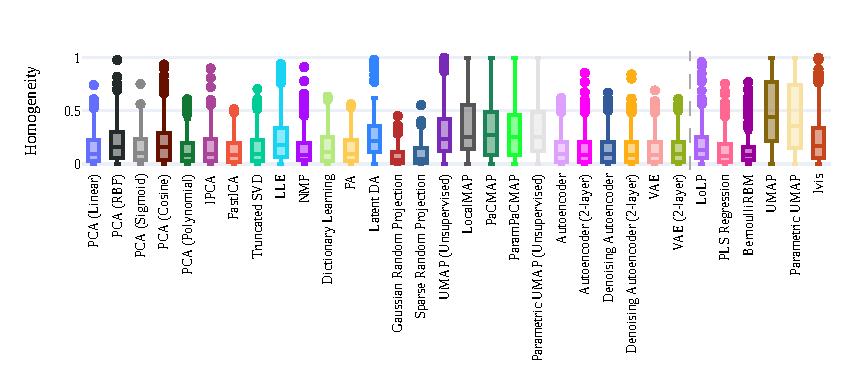
\includegraphics[width=\textwidth]{figures/04/ml/agg_10_homogeneity.pdf}
        \caption{\footnotesize{$k = 10$; homogeneity}}
    \end{subfigure}
    \begin{subfigure}{0.24\textwidth}
        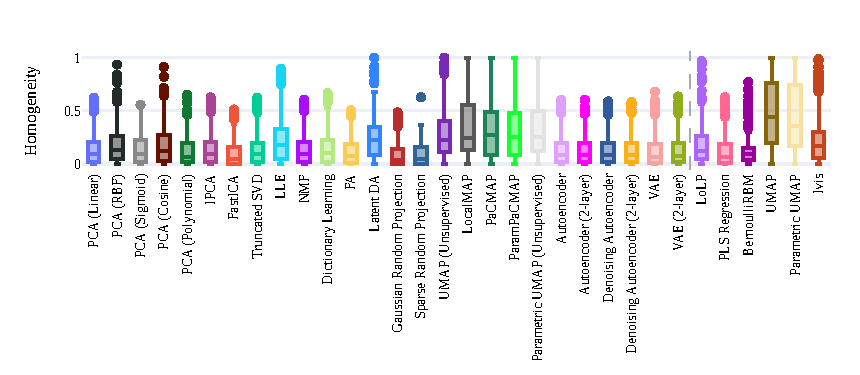
\includegraphics[width=\textwidth]{figures/04/ml/agg_20_homogeneity.pdf}
        \caption{\footnotesize{$k = 20$; homogeneity}}
    \end{subfigure}
    \begin{subfigure}{0.24\textwidth}
        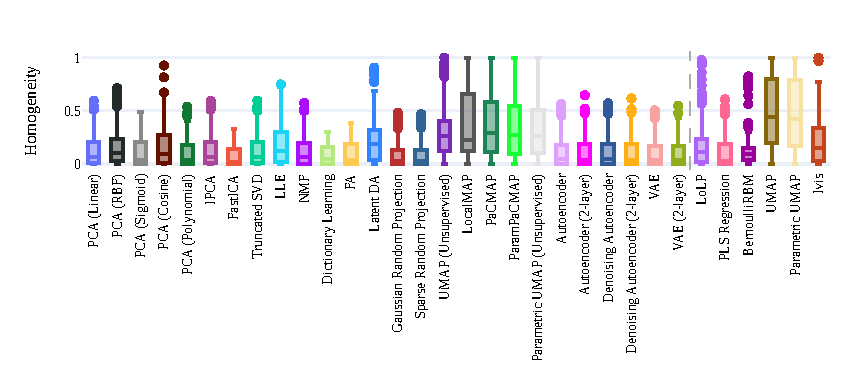
\includegraphics[width=\textwidth]{figures/04/ml/agg_40_homogeneity.pdf}
        \caption{\footnotesize{$k = 40$; homogeneity}}
    \end{subfigure}
    \begin{subfigure}{0.24\textwidth}
        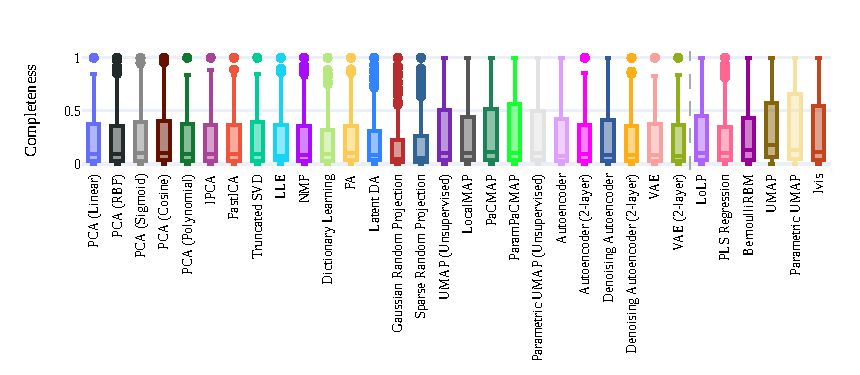
\includegraphics[width=\textwidth]{figures/04/ml/agg_5_completeness.pdf}
        \caption{\footnotesize{$k = 5$; completeness}}
    \end{subfigure}
    \begin{subfigure}{0.24\textwidth}
        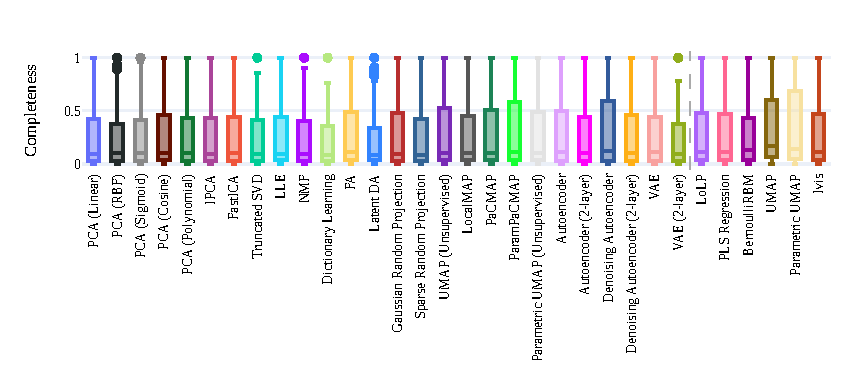
\includegraphics[width=\textwidth]{figures/04/ml/agg_10_completeness.pdf}
        \caption{\footnotesize{$k = 10$; completeness}}
    \end{subfigure}
    \begin{subfigure}{0.24\textwidth}
        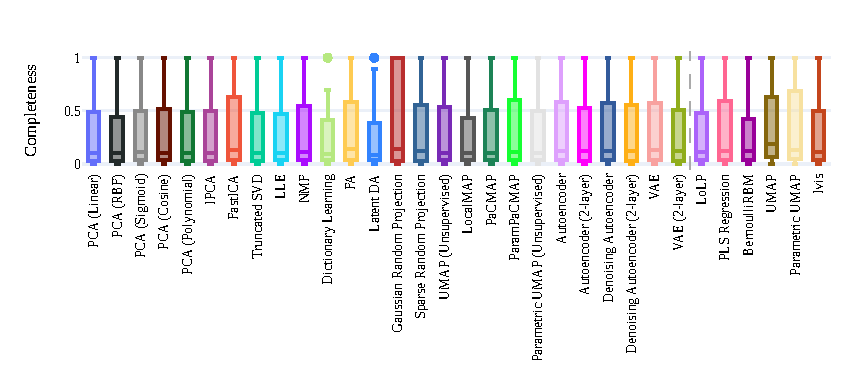
\includegraphics[width=\textwidth]{figures/04/ml/agg_20_completeness.pdf}
        \caption{\footnotesize{$k = 20$; completeness}}
    \end{subfigure}
    \begin{subfigure}{0.24\textwidth}
        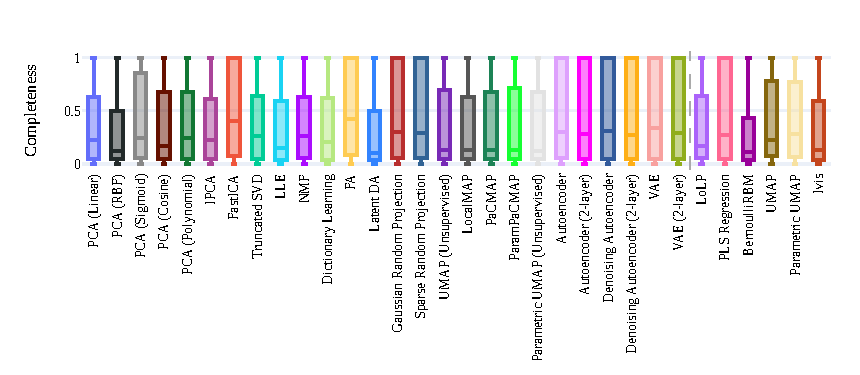
\includegraphics[width=\textwidth]{figures/04/ml/agg_40_completeness.pdf}
        \caption{\footnotesize{$k = 40$; completeness}}
    \end{subfigure}




















\caption[Clustering homogeneity and completeness on ML task 1]{

Performance of different dimensionality reduction methods aggregated across all OpenML~CC-18 datasets, for different target dimensionalities $k$, in terms of (a-d) cluster homogeneity and (e-h) cluster completeness on \textbf{machine learning task 1: clustering ability}; higher is better. Homogeneity measures whether each cluster contains samples from the same true class; we observe very small homogeneity differences between dimensionality reduction methods for different target dimensionalities. Completeness quantifies whether all samples belonging to the same true class are in the same cluster; we observe a slight improvement in performance measured by completeness as the target dimensionality increases.

}
\label{fig:ch04:cluster_all_agg}
\end{figure}

We now investigate the effect of input dimensionality by grouping the datasets into three categories based on their number of features: low- (up to 60 features), medium- (60–200 features), and high-dimensional datasets (more than 200 features). The results are presented in \cref{fig:ch04:cluster_homogeneity_dataset_sizes}.
We observe that LLE performs increasingly well on both metrics as the input dimensionality grows, reaching its best performance on medium-dimensional datasets.


This is possibly due to interference between the fact that some dimensions are irrelevant in the large-sized datasets and the estimation of a local neighbourhood.




With respect to cluster completeness, sparse random projection performs best on medium-dimensional data, whereas Gaussian random projection becomes the strongest method for large input dimensionalities, likely due to its ability to better preserve pairwise distances in high dimensions, consistent with the Johnson–Lindenstrauss effect.
Furthermore, dense Gaussian random projections handle large feature spaces better than sparse ones, avoiding information loss in very high dimensions.

\begin{figure}
\centering
    \begin{subfigure}{0.32\textwidth}
        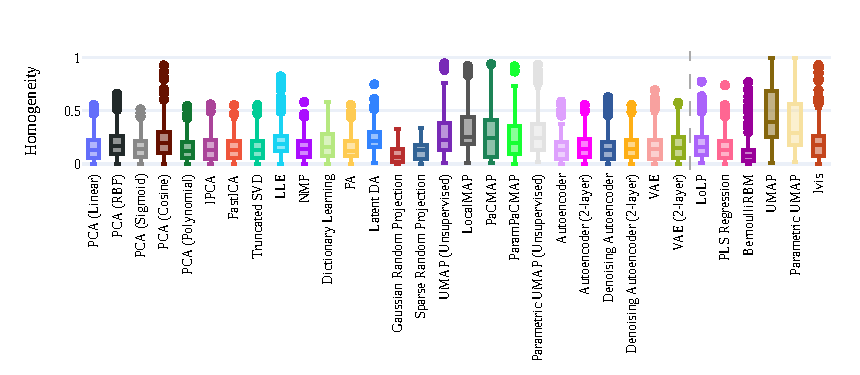
\includegraphics[width=\textwidth]{figures/04/ml/agg_small_5_homogeneity.pdf}
        \caption{Small $D$; homogeneity}
    \end{subfigure}
    \begin{subfigure}{0.32\textwidth}
        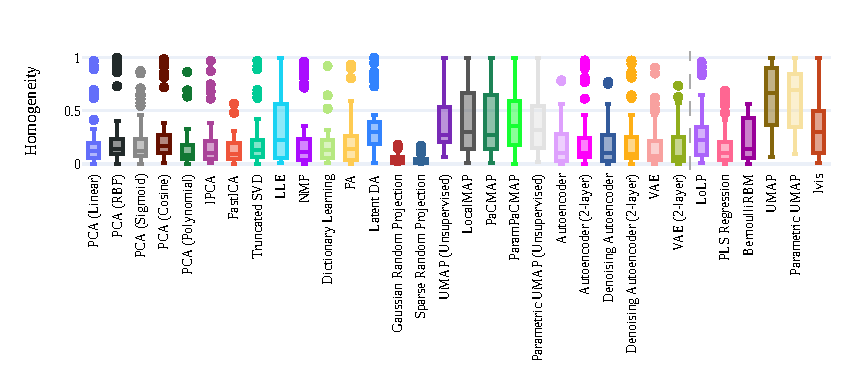
\includegraphics[width=\textwidth]{figures/04/ml/agg_medium_5_homogeneity.pdf}
        \caption{Medium $D$; homogeneity}
    \end{subfigure}
    \begin{subfigure}{0.32\textwidth}
        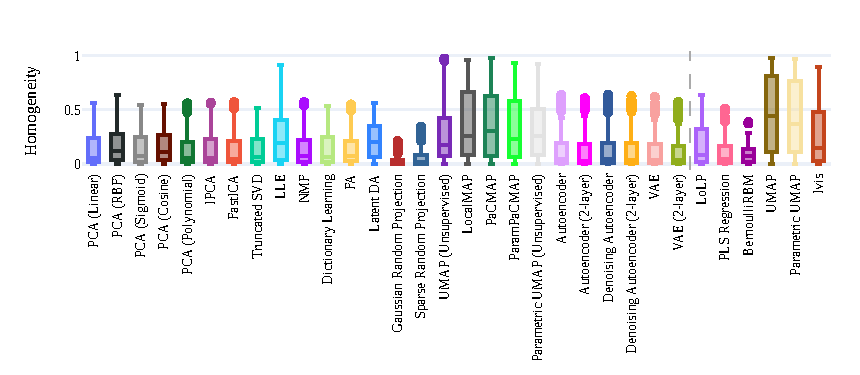
\includegraphics[width=\textwidth]{figures/04/ml/agg_large_5_homogeneity.pdf}
        \caption{Large $D$; homogeneity}
    \end{subfigure}
    \begin{subfigure}{0.32\textwidth}
        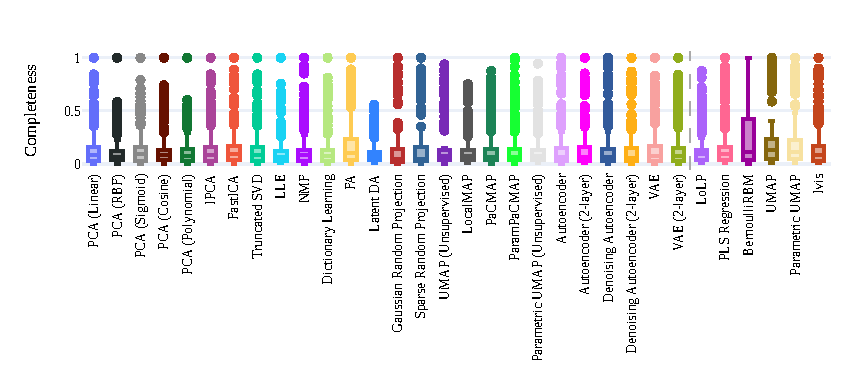
\includegraphics[width=\textwidth]{figures/04/ml/agg_small_5_completeness.pdf}
        \caption{Small $D$; completeness}
    \end{subfigure}
    \begin{subfigure}{0.32\textwidth}
        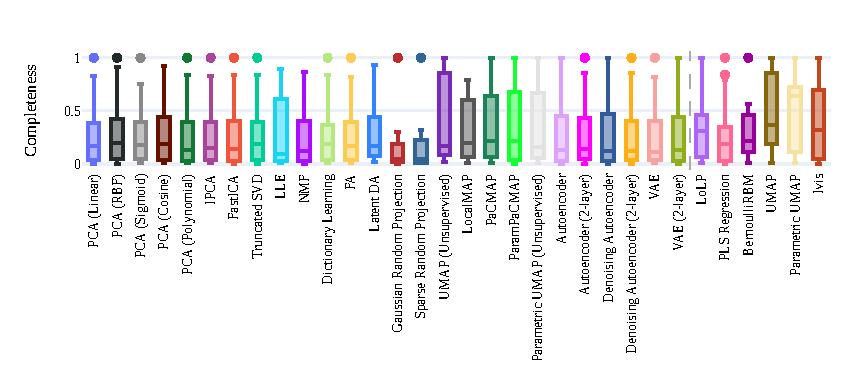
\includegraphics[width=\textwidth]{figures/04/ml/agg_medium_5_completeness.pdf}
        \caption{Medium $D$; completeness}
    \end{subfigure}
    \begin{subfigure}{0.32\textwidth}
        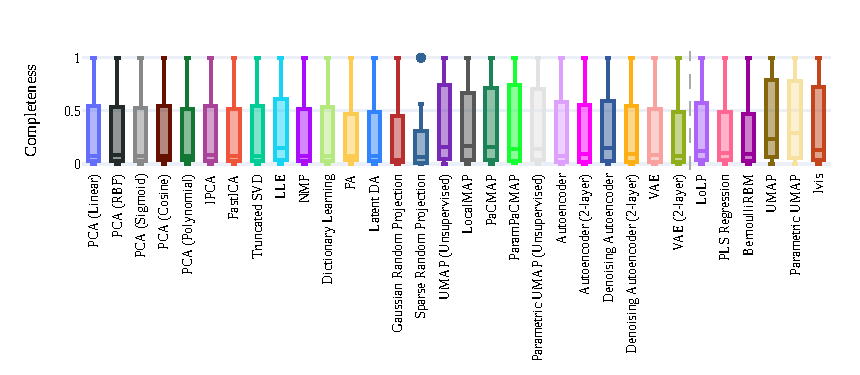
\includegraphics[width=\textwidth]{figures/04/ml/agg_large_5_completeness.pdf}
        \caption{Large $D$; completeness}
    \end{subfigure}
    \begin{subfigure}{0.32\textwidth}










    \end{subfigure}




\caption[Clustering on ML task 1 by dataset category]{

Performance of different dimensionality reduction methods on low-, medium- and high-dimensional OpenML~CC-18 datasets, all reduced to target dimensionality $k = 5$, in terms of (a-c) cluster homogeneity and (d-f) cluster completeness on \textbf{machine learning task 1: clustering ability}; higher is better. We observe a slightly larger improvement in completeness than in homogeneity as the dataset dimensionality increases.


}
\label{fig:ch04:cluster_homogeneity_dataset_sizes}
\end{figure}



\subsubsection*{Machine learning task 2: Tabular classification accuracy}



For the supervised machine learning task (\emph{i.e.,} prediction), 

we begin by analysing the results aggregated across all datasets and different machine learning models (random forest, gradient boosting, \gls{mlp}) for varying target dimensionalities $k$, as shown in \cref{fig:ch04:ml_pred_all}.
Across all models and methods, we observe that accuracy increases with the target dimensionality. 


In other words,


performance is lowest at $k=5$ and highest at $k=40$. 
This observation indicates that higher-dimensional projections retain more task-relevant information, allowing downstream models to make more accurate predictions.

Interestingly, while Gaussian and sparse random projection performed relatively well in the clustering task (particularly for cluster completeness), they rank among the worst-performing methods in the prediction task, only outperforming Bernoulli RBM. This suggests that although random projections preserve geometric structure, they do not necessarily retain the discriminative information required for predictive modelling.
Overall, while most methods achieve comparable accuracy, LoLP consistently performs best. This outcome is expected, as LoLP is explicitly designed to enhance predictive performance in machine learning settings, confirming its suitability for supervised downstream tasks.


\begin{figure}
\centering
    \begin{subfigure}{0.24\textwidth}
        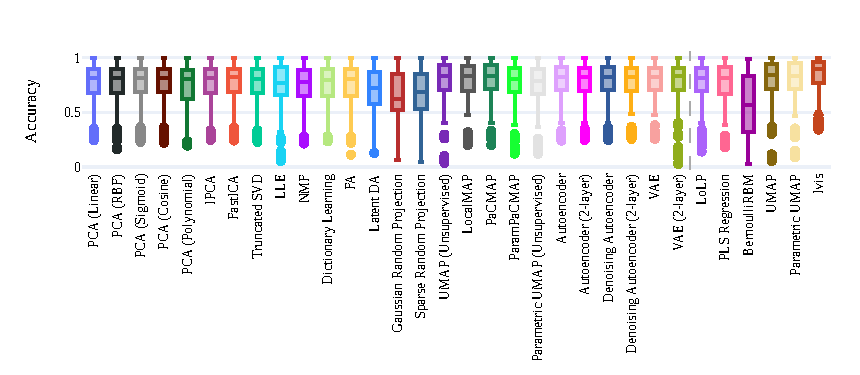
\includegraphics[width=\textwidth]{figures/04/ml/agg_5_rf_acc.pdf}
        \caption{\footnotesize Random Forest; $k = 5$}
    \end{subfigure}
    \begin{subfigure}{0.24\textwidth}
        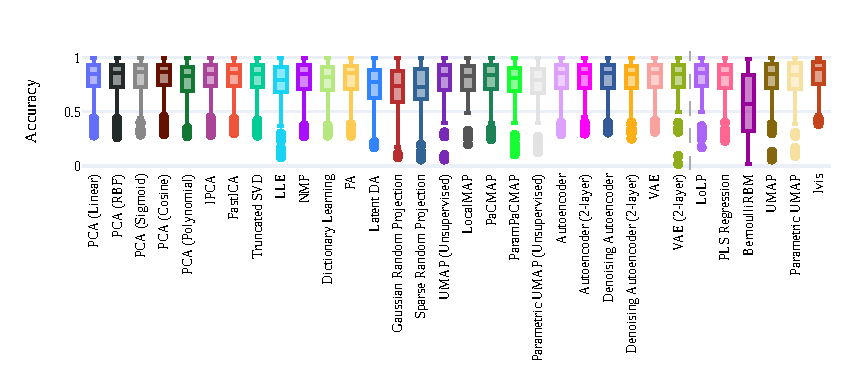
\includegraphics[width=\textwidth]{figures/04/ml/agg_10_rf_acc.pdf}
        \caption{\footnotesize Random Forest; $k = 10$}
    \end{subfigure}
    \begin{subfigure}{0.24\textwidth}
        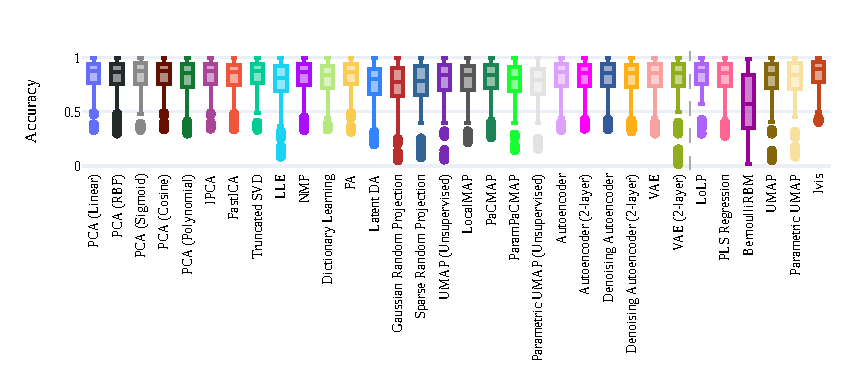
\includegraphics[width=\textwidth]{figures/04/ml/agg_20_rf_acc.pdf}
        \caption{\footnotesize Random Forest; $k = 20$}
    \end{subfigure}
    \begin{subfigure}{0.24\textwidth}
        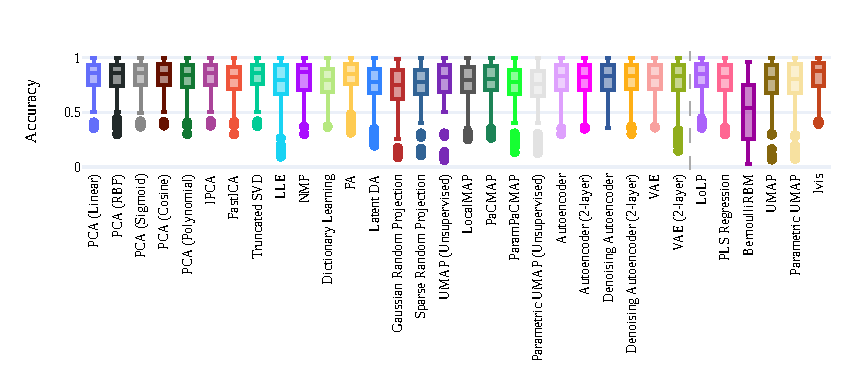
\includegraphics[width=\textwidth]{figures/04/ml/agg_40_rf_acc.pdf}
        \caption{\footnotesize Random Forest; $k = 40$}
    \end{subfigure}
    \begin{subfigure}{0.24\textwidth}
        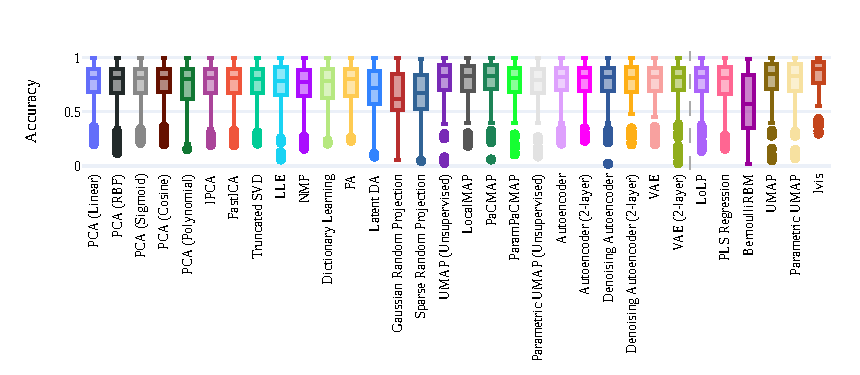
\includegraphics[width=\textwidth]{figures/04/ml/agg_5_gb_acc.pdf}
        \caption{\footnotesize Gradient Boosting; $k = 5$}
    \end{subfigure}
    \begin{subfigure}{0.24\textwidth}
        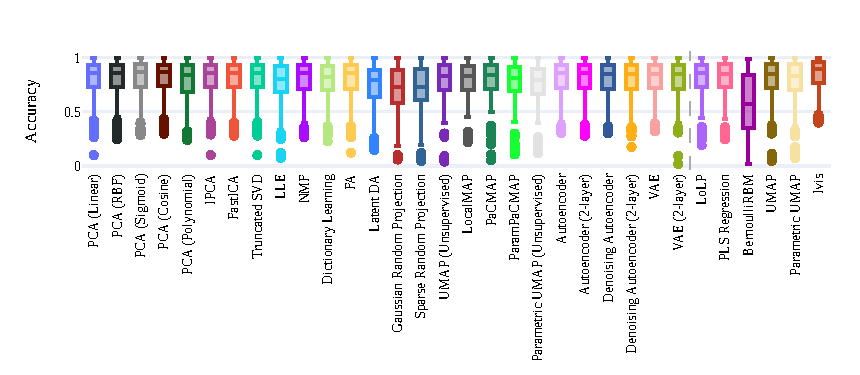
\includegraphics[width=\textwidth]{figures/04/ml/agg_10_gb_acc.pdf}
        \caption{\footnotesize Gradient Boosting; $k = 10$}
    \end{subfigure}
    \begin{subfigure}{0.24\textwidth}
        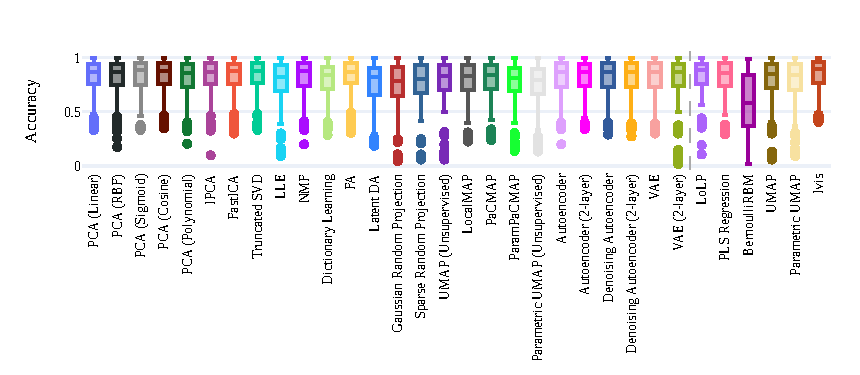
\includegraphics[width=\textwidth]{figures/04/ml/agg_20_gb_acc.pdf}
        \caption{\footnotesize Gradient Boosting; $k = 20$}
    \end{subfigure}
    \begin{subfigure}{0.24\textwidth}
        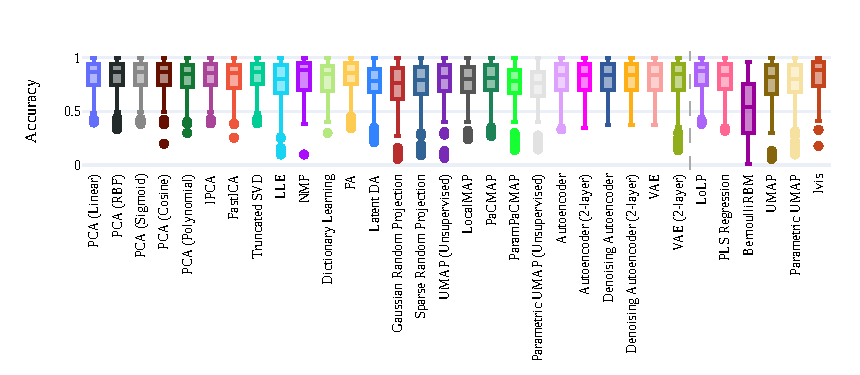
\includegraphics[width=\textwidth]{figures/04/ml/agg_40_gb_acc.pdf}
        \caption{\footnotesize Gradient Boosting; $k = 40$}
    \end{subfigure}
    \begin{subfigure}{0.24\textwidth}
        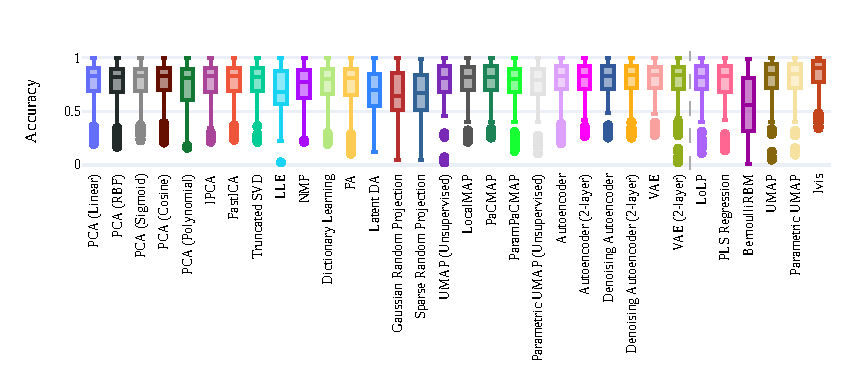
\includegraphics[width=\textwidth]{figures/04/ml/agg_5_mlp_acc.pdf}
        \caption{\footnotesize \gls{mlp}; $k = 5$}
    \end{subfigure}
    \begin{subfigure}{0.24\textwidth}
        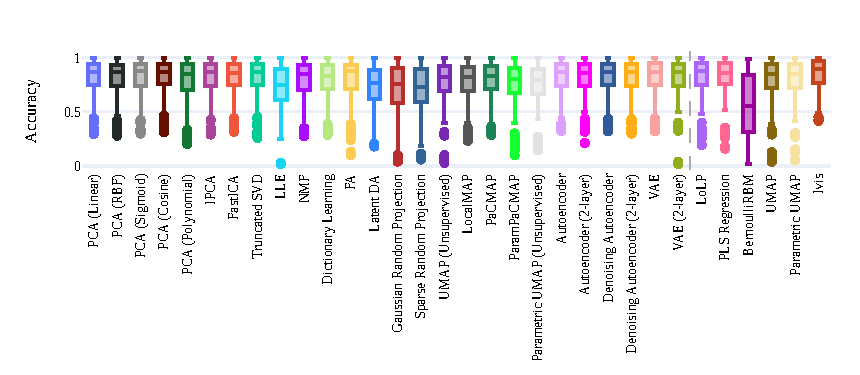
\includegraphics[width=\textwidth]{figures/04/ml/agg_10_mlp_acc.pdf}
        \caption{\footnotesize \gls{mlp}; $k = 10$}
    \end{subfigure}
    \begin{subfigure}{0.24\textwidth}
        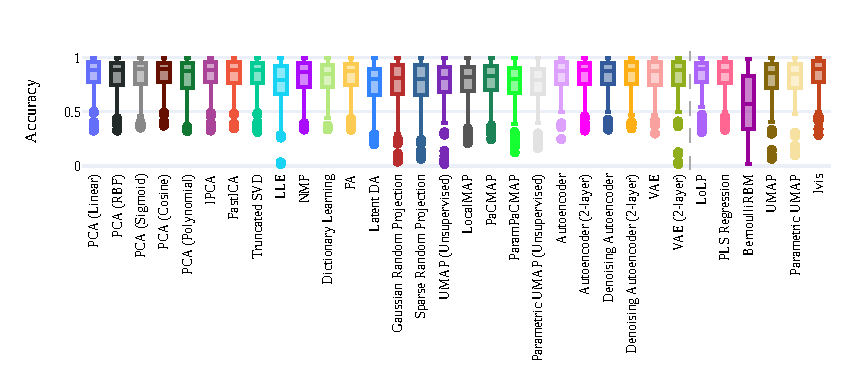
\includegraphics[width=\textwidth]{figures/04/ml/agg_20_mlp_acc.pdf}
        \caption{\footnotesize \gls{mlp}; $k = 20$}
    \end{subfigure}
    \begin{subfigure}{0.24\textwidth}
        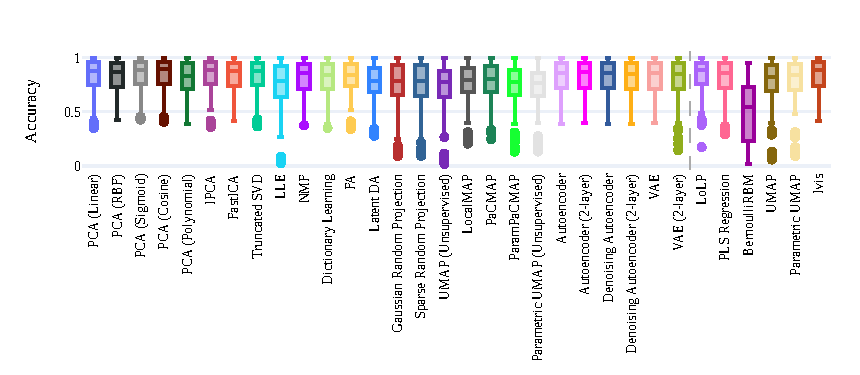
\includegraphics[width=\textwidth]{figures/04/ml/agg_40_mlp_acc.pdf}
        \caption{\footnotesize \gls{mlp}; $k = 40$}
    \end{subfigure}




\caption[Classification accuracy on ML task 2]{

Performance of different dimensionality reduction methods aggregated across all OpenML~CC-18 datasets, for different target dimensionalities $k$ and for different machine learning models used for classification (random forest, gradient boosting, \gls{mlp}), in terms of accuracy on \textbf{machine learning task 2: tabular classification accuracy}; higher is better. Bernoulli RBM performs consistently bad across all settings, followed by Gaussian and sparse random projections, while LoLP exhibits a consistent slight performance edge over other methods.

}
\label{fig:ch04:ml_pred_all}
\end{figure}

We conclude our analysis of the machine learning tasks by examining the results of the prediction task across different dataset sizes, following the same procedure as for the clustering task. We fix the target dimensionality to $k=5$.

We first observe that Bernoulli RBM, Gaussian and sparse random projections show strongly degraded performance as the number of features increases. Even on the low-dimensional datasets, these methods already underperform compared to other approaches, suggesting that they increasingly fail to preserve essential information needed for predictive modelling as dataset dimensionality increases.
In contrast, PCA (Linear) and PCA (Polynomial) perform better than other PCA variants on low-dimensional datasets. This behaviour likely reflects that linear and low-order polynomial relationships are sufficient to capture the main predictive variance in smaller feature spaces, while more complex kernels (such as RBF or Cosine) become beneficial only in higher-dimensional spaces.

\begin{figure}
\centering
    \begin{subfigure}{0.32\textwidth}
        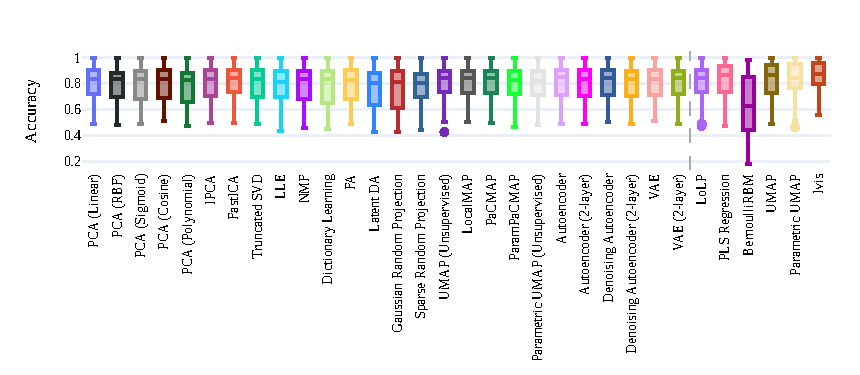
\includegraphics[width=\textwidth]{figures/04/ml/agg_small_5_rf_acc.pdf}
        \caption{Small $D$; Random Forest}
    \end{subfigure}
    \begin{subfigure}{0.32\textwidth}
        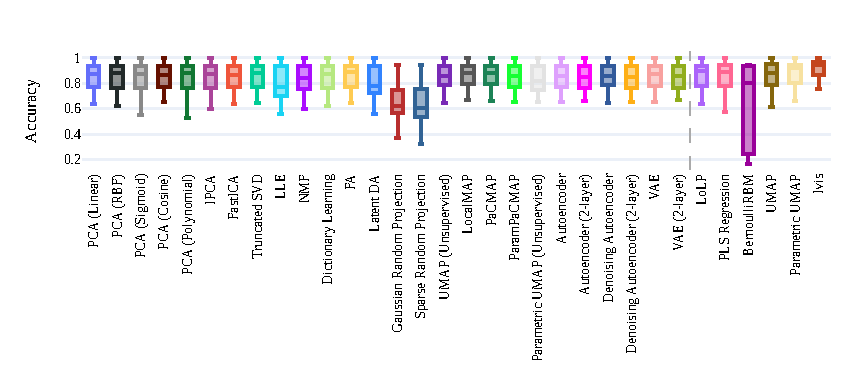
\includegraphics[width=\textwidth]{figures/04/ml/agg_medium_5_rf_acc.pdf}
        \caption{Medium $D$; Random Forest}
    \end{subfigure}
    \begin{subfigure}{0.32\textwidth}
        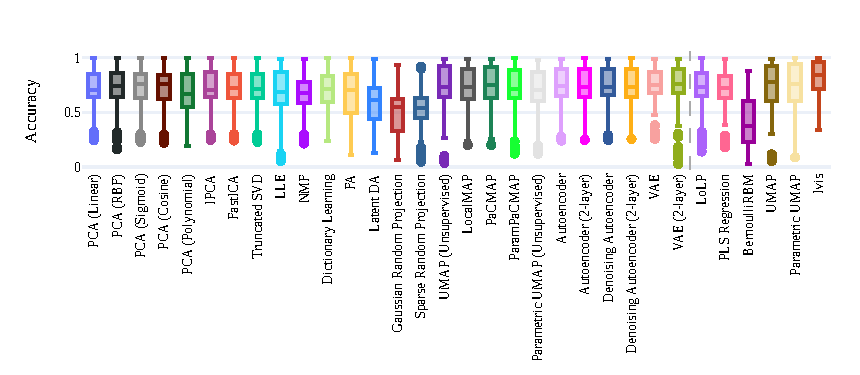
\includegraphics[width=\textwidth]{figures/04/ml/agg_large_5_rf_acc.pdf}
        \caption{Large $D$; Random Forest}
    \end{subfigure}
    \begin{subfigure}{0.32\textwidth}
        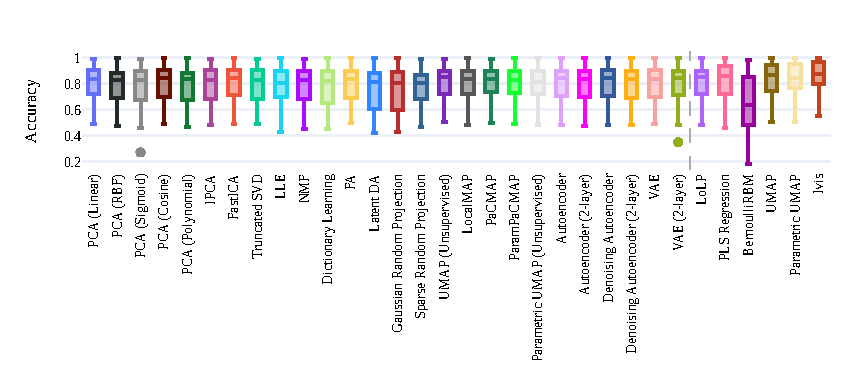
\includegraphics[width=\textwidth]{figures/04/ml/agg_small_5_gb_acc.pdf}
        \caption{Small $D$; Gradient Boosting}
    \end{subfigure}
    \begin{subfigure}{0.32\textwidth}
        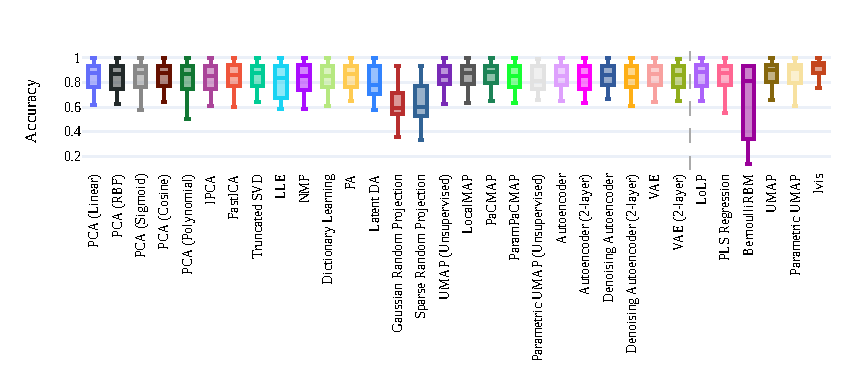
\includegraphics[width=\textwidth]{figures/04/ml/agg_medium_5_gb_acc.pdf}
        \caption{Medium $D$; Gradient Boosting}
    \end{subfigure}
    \begin{subfigure}{0.32\textwidth}
        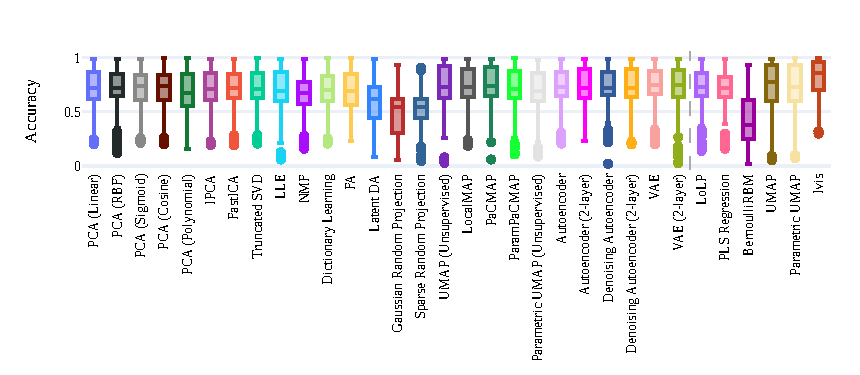
\includegraphics[width=\textwidth]{figures/04/ml/agg_large_5_gb_acc.pdf}
        \caption{Large $D$; Gradient Boosting}
    \end{subfigure}
    \begin{subfigure}{0.32\textwidth}
        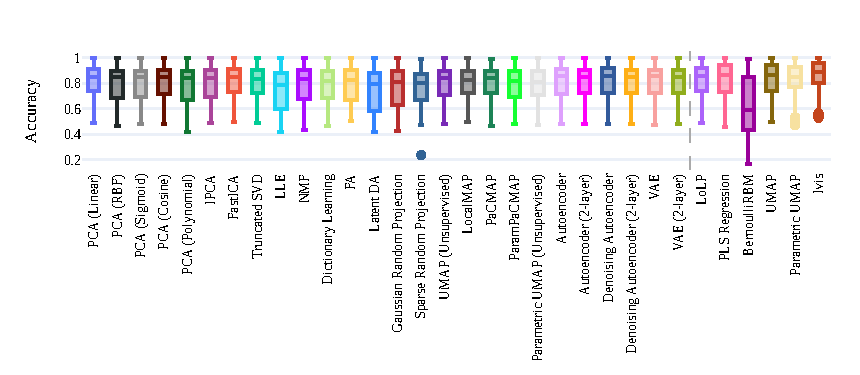
\includegraphics[width=\textwidth]{figures/04/ml/agg_small_5_mlp_acc.pdf}
        \caption{Small $D$; \gls{mlp}}
    \end{subfigure}
    \begin{subfigure}{0.32\textwidth}
        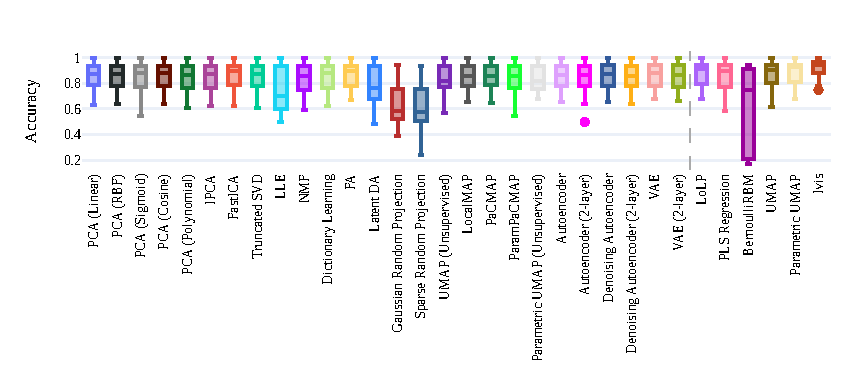
\includegraphics[width=\textwidth]{figures/04/ml/agg_medium_5_mlp_acc.pdf}
        \caption{Medium $D$; \gls{mlp}}
    \end{subfigure}
    \begin{subfigure}{0.32\textwidth}
        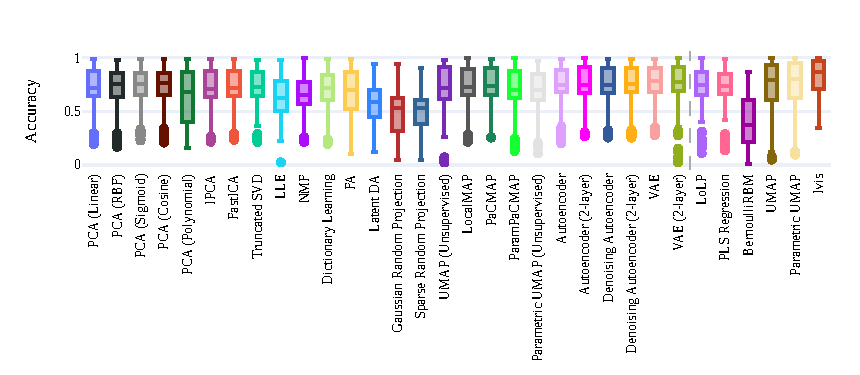
\includegraphics[width=\textwidth]{figures/04/ml/agg_large_5_mlp_acc.pdf}
        \caption{Large $D$; \gls{mlp}}
    \end{subfigure}





\caption[Classification accuracy on ML task 2 by dataset category]{

Performance of different dimensionality reduction methods on low-, medium- and high-dimensional OpenML~CC-18 datasets, all reduced to target dimensionality $k = 5$, in terms of accuracy on \textbf{machine learning task 2: tabular classification accuracy}, where classification is done using different machine learning models (random forest, gradient boosting, \gls{mlp}); higher is better. The performance of Bernoulli RBM and Gaussian and sparse random projection degrades even further as the dataset dimensionality increases, regardless of the machine learning model used for classification. The differences induced by the choice of the machine learning model are generally negligible for low-, medium- and high-dimensional datasets alike.

}
\label{fig:ch04:ml_pred_sizes}
\end{figure}


\subsection{Black-box optimisation tasks}
\label{sec:ch04:res-bbo}

\subsubsection*{Black-box optimisation task 1: Target function approximation}






\begin{figure}
    \centering
    \begin{subfigure}[t]{0.24\textwidth}
        \centering
        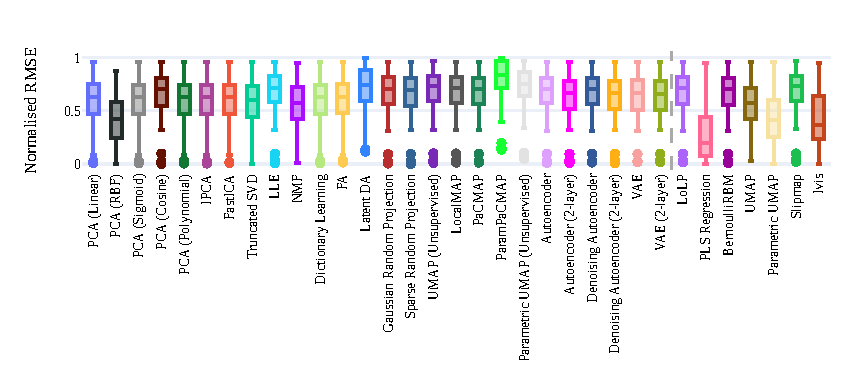
\includegraphics[width=\textwidth]{figures/04/epm/agg_sample_red_inpt_100_120_5.pdf}
        \caption{$k=5$}
    \end{subfigure}
    \begin{subfigure}[t]{0.24\textwidth}
        \centering
        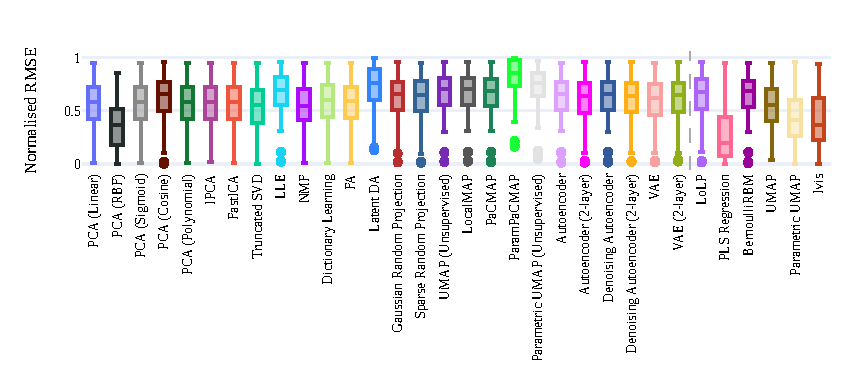
\includegraphics[width=\textwidth]{figures/04/epm/agg_sample_red_inpt_100_120_10.pdf}
        \caption{$k=10$}
    \end{subfigure}
    \begin{subfigure}[t]{0.24\textwidth}
        \centering
        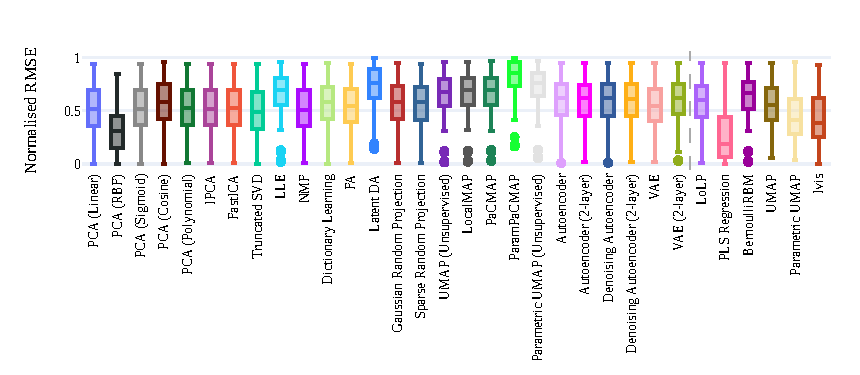
\includegraphics[width=\textwidth]{figures/04/epm/agg_sample_red_inpt_100_120_20.pdf}
        \caption{$k=20$}
    \end{subfigure}
    \begin{subfigure}[t]{0.24\textwidth}
        \centering
        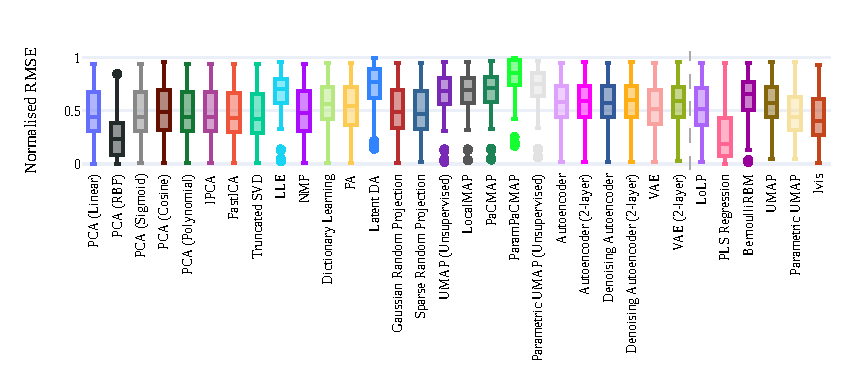
\includegraphics[width=\textwidth]{figures/04/epm/agg_sample_red_inpt_100_120_40.pdf}
        \caption{$k=40$}
    \end{subfigure}
    \caption[Target function approximation on BBO task 1]{

    Performance of different dimensionality reduction methods aggregated across synthetic benchmark problems for different target dimensionalities $k$, with input dimensionality $D = 120$ and initial sample size $N = 100$, in terms of min-max normalised mean \gls{rmse} on \textbf{black-box optimisation task 1: target function approximation}; lower is better. 
    PLS regression consistently performs best across different target dimensionalities, and is closely followed by PCA (RBF) for the highest target dimensionality.



    }
    \label{fig:ch04:res-bbo-task1_red_dim_inpt_dim}
\end{figure}


We focus on a selection of representative aggregated results to simplify analysis.
We start by looking into the results on synthetic benchmarks for black-box optimisation task 1.


First, we examine the effect of varying the target dimensionality $k$ in \cref{fig:ch04:res-bbo-task1_red_dim_inpt_dim}, keeping the input dimensionality fixed at $D = 120$ and the initial sample size at $N = 100$.
Across all target dimensionalities, and particularly in the low-dimensional setting, PLS regression consistently performs best. 
This aligns with expectations, as PLS components are explicitly optimised to maximise the predictive power of the target variables, which is especially suitable when dimensionality reduction is used as a preprocessing step for regression. 

As the target dimensionality increases, PCA (RBF) gradually catches up and eventually performs on par with PLS regression. More generally, all PCA variants improve their relative performance with higher target dimensionalities, likely because higher-dimensional projections preserve more variance and structure from the original data, even without explicit supervision.



\begin{figure}
\begin{subfigure}[t]{0.32\textwidth}
        \centering
        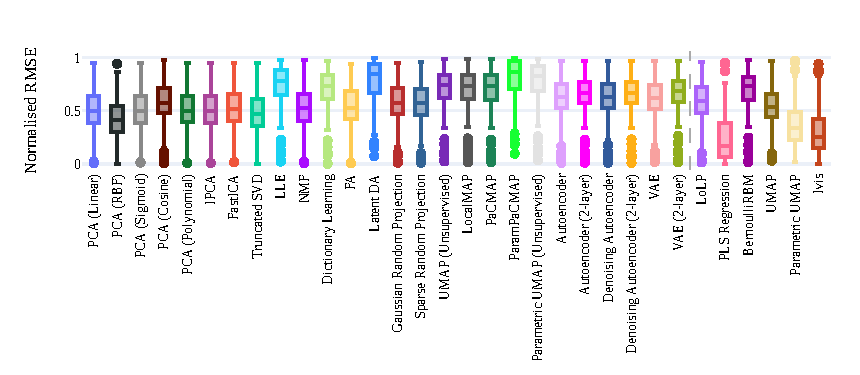
\includegraphics[width=\textwidth]{figures/04/epm/agg_sample_red_inpt_100_40_20.pdf}
        \caption{$D=40$}
    \end{subfigure}
    \begin{subfigure}[t]{0.32\textwidth}
        \centering
        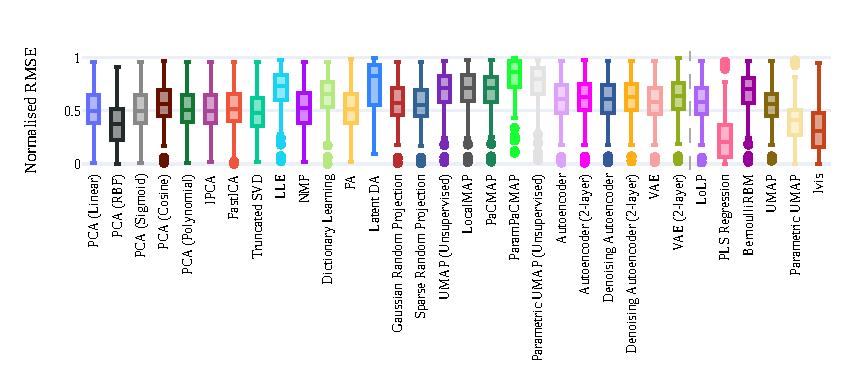
\includegraphics[width=\textwidth]{figures/04/epm/agg_sample_red_inpt_100_60_20.pdf}
        \caption{$D=60$}
    \end{subfigure}
    \begin{subfigure}[t]{0.32\textwidth}
        \centering
        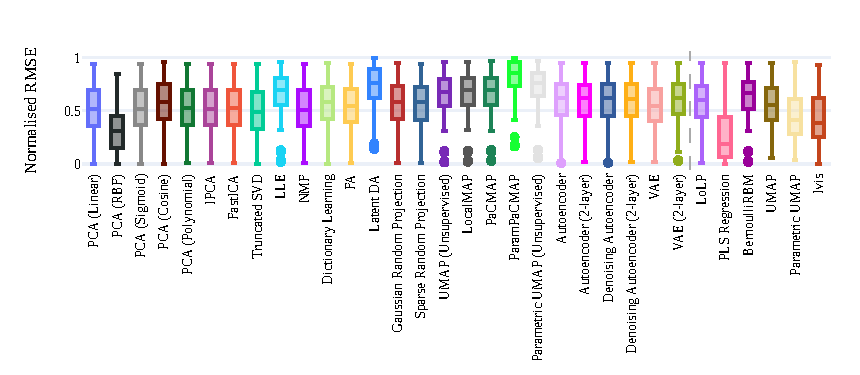
\includegraphics[width=\textwidth]{figures/04/epm/agg_sample_red_inpt_100_120_20.pdf}
        \caption{$D=120$}
    \end{subfigure}
    \begin{subfigure}[t]{0.32\textwidth}
        \centering
        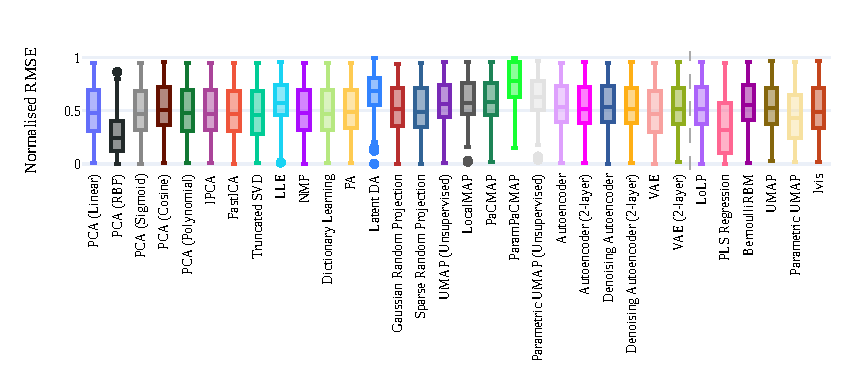
\includegraphics[width=\textwidth]{figures/04/epm/agg_sample_red_inpt_100_240_20.pdf}
        \caption{$D=240$}
    \end{subfigure}
    \begin{subfigure}[t]{0.32\textwidth}
        \centering
        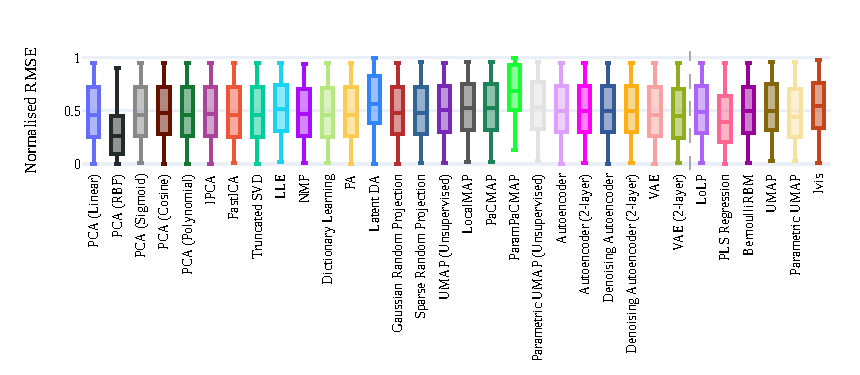
\includegraphics[width=\textwidth]{figures/04/epm/agg_sample_red_inpt_100_500_20.pdf}
        \caption{$D=500$}
    \end{subfigure}
    \begin{subfigure}[t]{0.32\textwidth}
        \centering
        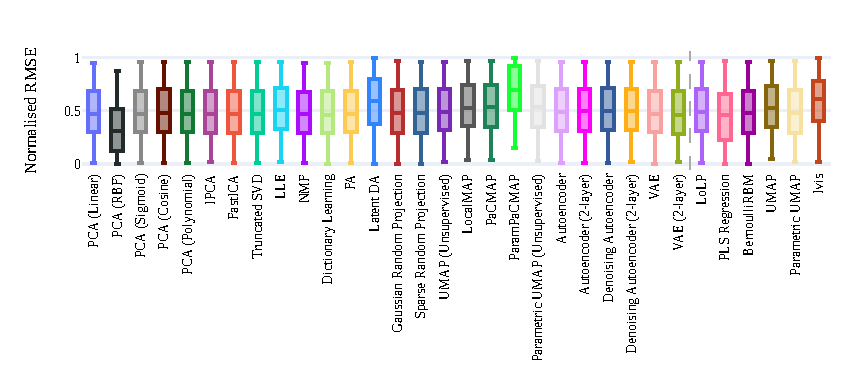
\includegraphics[width=\textwidth]{figures/04/epm/agg_sample_red_inpt_100_1000_20.pdf}
        \caption{$D=1000$}
    \end{subfigure}
    \hspace{0.2cm}
    \begin{subfigure}[t]{0.8\textwidth}
        \centering
        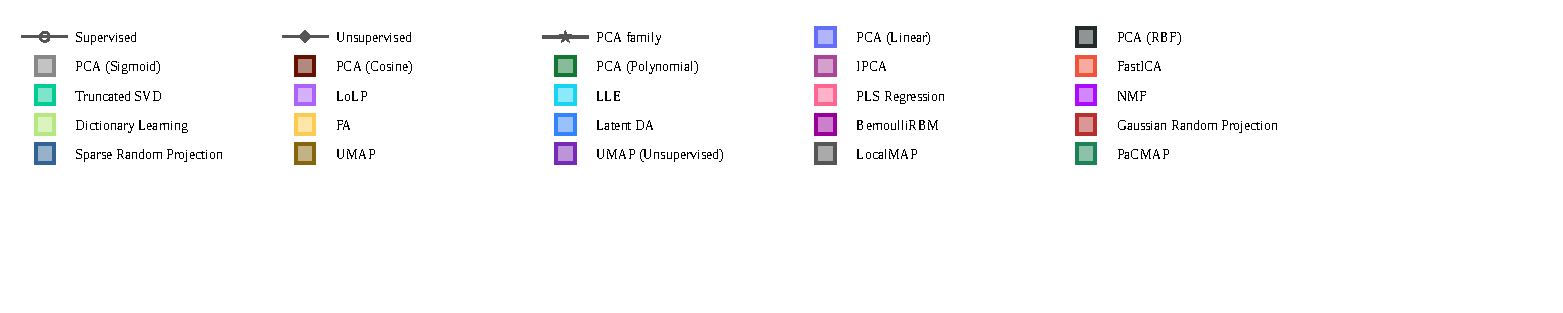
\includegraphics[width=1.0\textwidth,trim={1.5cm 4cm 3.7cm 0.0cm},clip]{figures/04/legend.pdf}
    \end{subfigure}
    \caption[Target function approximation on BBO task 1 for real-world benchmarks]{

    Performance of different dimensionality reduction methods aggregated across synthetic benchmark problems for different input dimensionalities $D$, with target dimensionality $k = 20$ and initial sample size $N = 100$, in terms of min-max normalised mean \gls{rmse} on \textbf{black-box optimisation task 1: target function approximation}; lower is better. 
    The variance increases with input dimensionality; PLS regression is a dominant method for lower-dimensional inputs (a-c), but is outperformed by PCA (RBF) for higher-dimensional inputs (d-f).


    }
    \label{fig:ch04:res-bbo-task1_inpt_dim}
\end{figure}



Second, we look into the effect of varying the input dimensionality $D$, keeping the target dimensionality fixed at $k = 20$ and the initial sample size at $N = 100$. This is illustrated in~\cref{fig:ch04:res-bbo-task1_inpt_dim}.


As expected, the variance of all methods decreases with lower input dimensionality, reflecting the reduced complexity of the search space. In this setting (up to ~120 input dimensions), PLS regression consistently outperforms other methods, leveraging its ability to extract components that are directly predictive of the targets. Conversely, for higher input dimensionalities, PCA (RBF) becomes the dominant method, likely because it captures more of the underlying variance and non-linear structure that PLS regression cannot exploit efficiently in very high-dimensional spaces. Together with previous findings, this suggests that PLS regression is best when both input and output dimensions are small, while PCA (RBF) is more suitable for high-dimensional settings.



\begin{figure}
    \centering
    \begin{subfigure}[t]{0.24\textwidth}
        \centering
        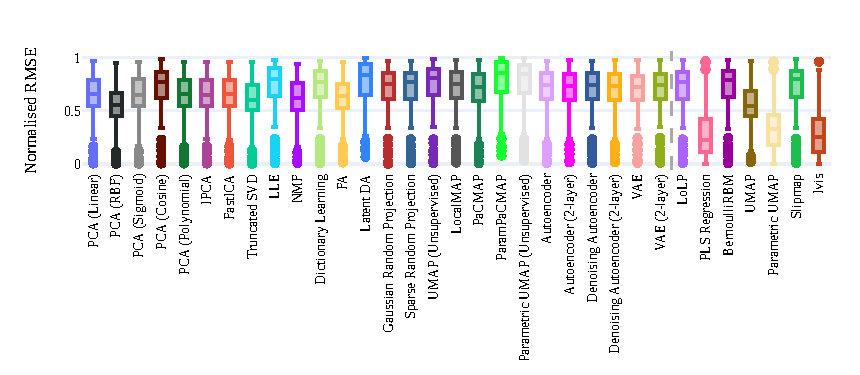
\includegraphics[width=\textwidth]{figures/04/epm/agg_sample_red_inpt_100_40_5}
        \caption{\footnotesize$D = 40, k = 5, N = 100$}
    \end{subfigure}
    \begin{subfigure}[t]{0.24\textwidth}
        \centering
        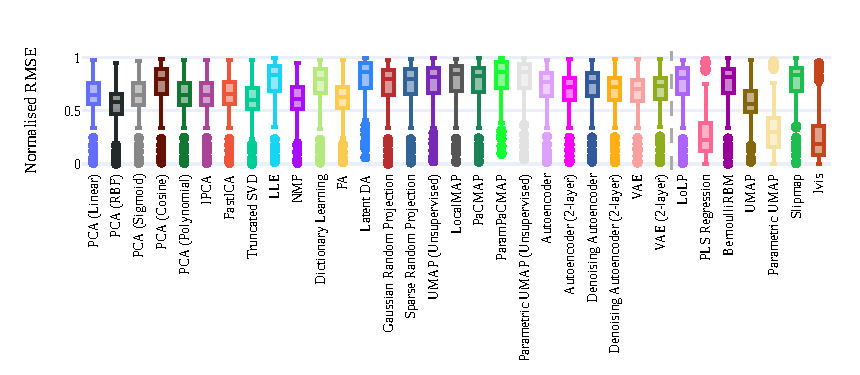
\includegraphics[width=\textwidth]{figures/04/epm/agg_sample_red_inpt_200_40_5.pdf}
        \caption{\footnotesize$D = 40, k = 5, N = 200$}
    \end{subfigure}
    \begin{subfigure}[t]{0.24\textwidth}
        \centering
        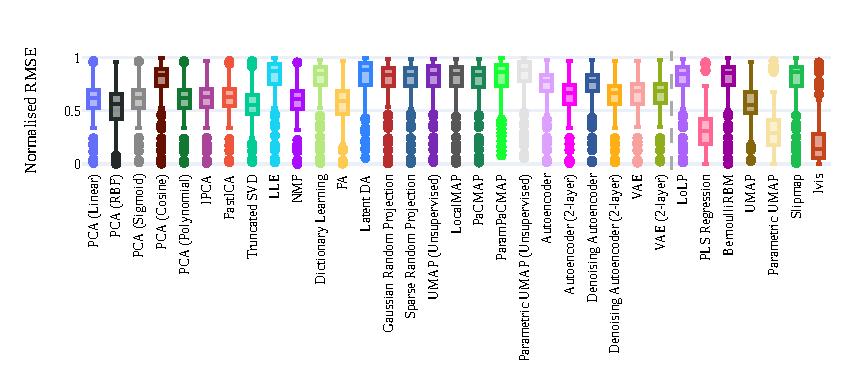
\includegraphics[width=\textwidth]{figures/04/epm/agg_sample_red_inpt_500_40_5.pdf}
        \caption{\footnotesize$D = 40, k = 5, N = 500$}
    \end{subfigure}
    \begin{subfigure}[t]{0.24\textwidth}
        \centering
        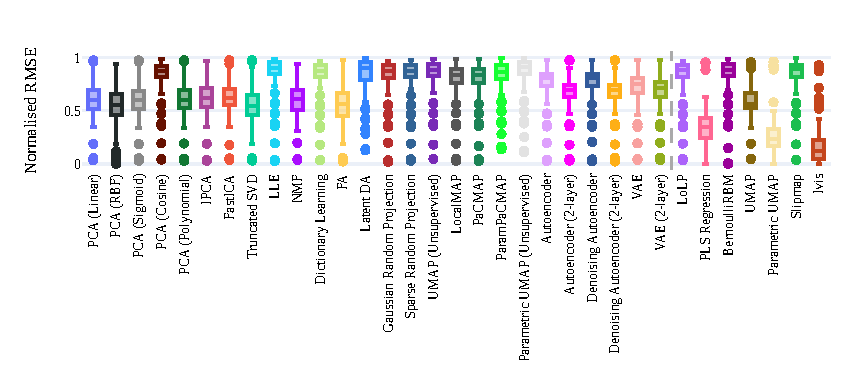
\includegraphics[width=\textwidth]{figures/04/epm/agg_sample_red_inpt_1000_40_5.pdf}
        \caption{\footnotesize$D = 40, k = 5, N = 1000$}
    \end{subfigure}
    \begin{subfigure}[t]{0.24\textwidth}
        \centering
        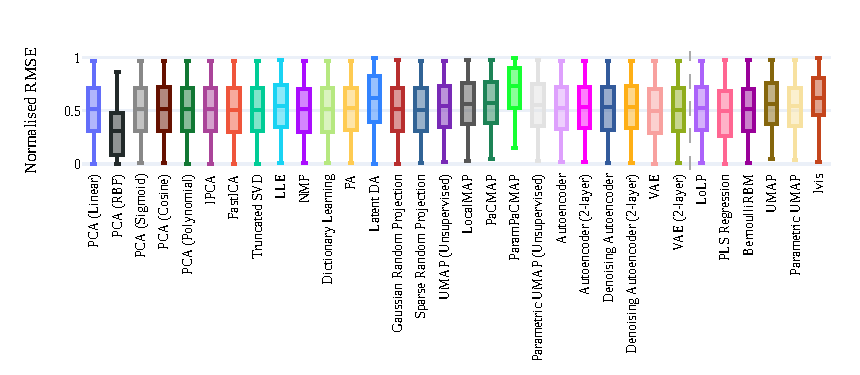
\includegraphics[width=\textwidth]{figures/04/epm/agg_sample_red_inpt_100_1000_40.pdf}
        \caption{\footnotesize$D = 1000, k = 40, N = 100$}
    \end{subfigure}
    \begin{subfigure}[t]{0.24\textwidth}
        \centering
        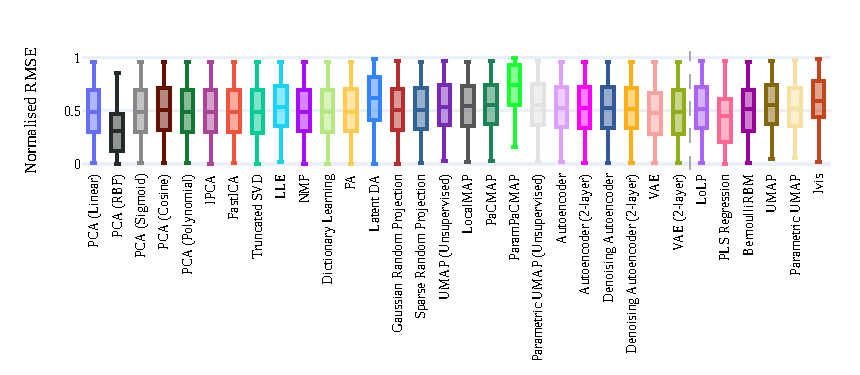
\includegraphics[width=\textwidth]{figures/04/epm/agg_sample_red_inpt_200_1000_40.pdf}
        \caption{\footnotesize$D = 1000, k = 40, N = 200$}
    \end{subfigure}
    \begin{subfigure}[t]{0.24\textwidth}
        \centering
        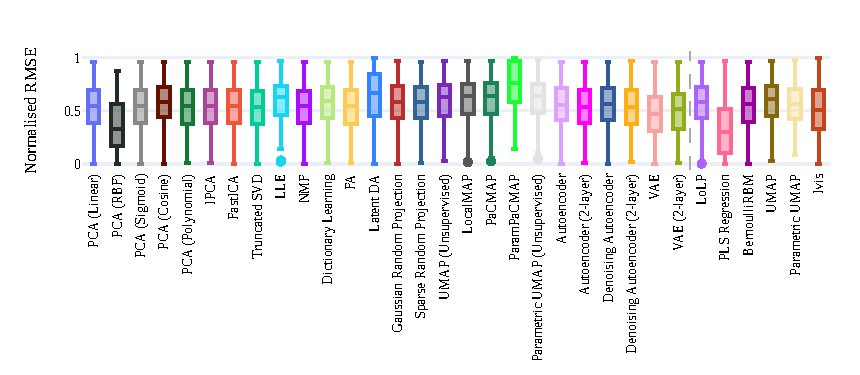
\includegraphics[width=\textwidth]{figures/04/epm/agg_sample_red_inpt_500_1000_40.pdf}
        \caption{\footnotesize$D = 1000, k = 40, N = 500$}
    \end{subfigure}
    \begin{subfigure}[t]{0.24\textwidth}
        \centering
        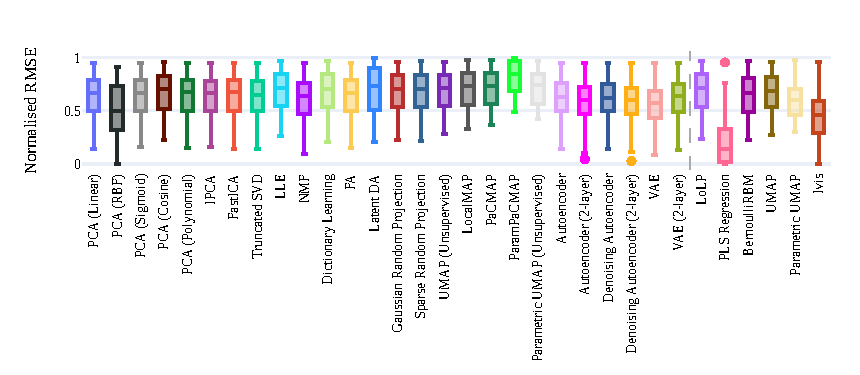
\includegraphics[width=\textwidth]{figures/04/epm/agg_sample_red_inpt_1000_1000_40.pdf}
        \caption{\footnotesize$D = 1000, k = 40, N = 1000$}
    \end{subfigure}
    \hspace{0.2cm}
    \begin{subfigure}[t]{0.8\textwidth}
        \centering
        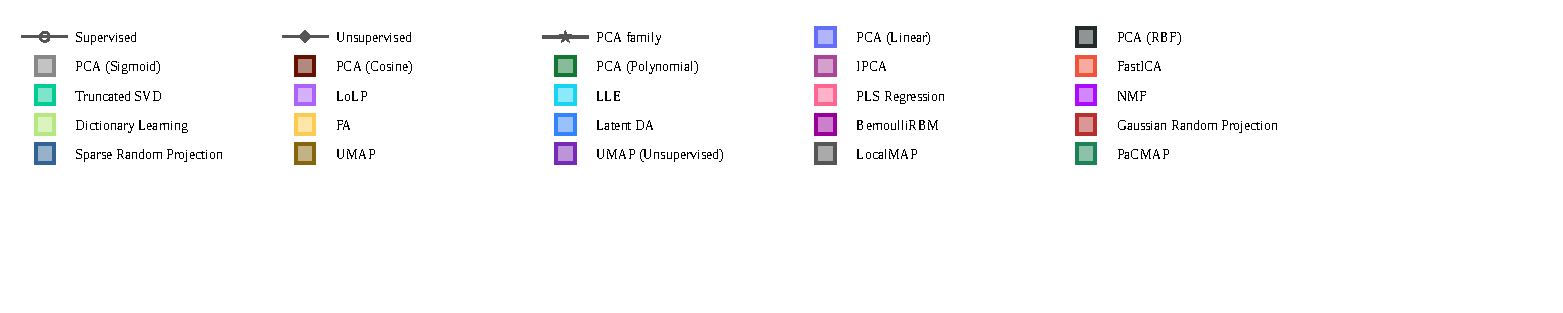
\includegraphics[width=1.0\textwidth,trim={1.5cm 4cm 3.7cm 0.0cm},clip]{figures/04/legend.pdf}
    \end{subfigure}
    \caption[Target function approximation quality by dimensionality]{

    Performance of different dimensionality reduction methods aggregated across synthetic benchmark problems for different initial sample sizes $N$ in two settings: (a-d) with input dimensionality $D = 40$ and target dimensionality $k = 5$, and (e-h) with input dimensionality $D = 1000$ and target dimensionality $k = 40$, in terms of min-max normalised mean \gls{rmse} on \textbf{black-box optimisation task 1: target function approximation}; lower is better.
    Initial sample size has almost no effect when the dimensionality reduction is performed from an already low-dimensional space into an even lower-dimensional one. On the other hand, for a more drastic dimensionality reduction from a very high-dimensional space into a relatively low-dimensional one, a large initial sample size is necessary for accurate target function approximation. 



    }
    \label{fig:ch04:res-bbo-task2_samp_sizes}
\end{figure}


We now analyse the effect of varying initial sample sizes for training dimensionality reduction methods. \cref{fig:ch04:res-bbo-task2_samp_sizes} shows the results aggregated across all different initial sample sizes ($N \in \{100, 200, 500, 1000\}$) for two settings: low-dimensional inputs ($D = 40$, target dimensionality $k = 5$; figures a–d) and high-dimensional inputs ($D = 1000$, target dimensionality $k = 40$; figures e–h).

For the low-dimensional setting ($D = 40$), performance is largely stable across different initial sample sizes. This stability likely arises due to the fact that even the smallest initial sample size already exceeds the number of input dimensions, providing sufficient information for reliable component extraction.
In contrast, for high-dimensional inputs ($D = 1000$), variance decreases noticeably as the initial sample size grows. With $1000$ samples used for dimensionality reduction training, the variance approaches levels observed in the low-dimensional case. This indicates that, although the dimensionality reduction methods are designed to work with limited data, they still depend on sufficient initial sample size (especially when input dimensionality is large) to produce stable and reliable results in predictive tasks.

\begin{figure}
    \centering
    \begin{subfigure}[t]{0.24\textwidth}
        \centering
        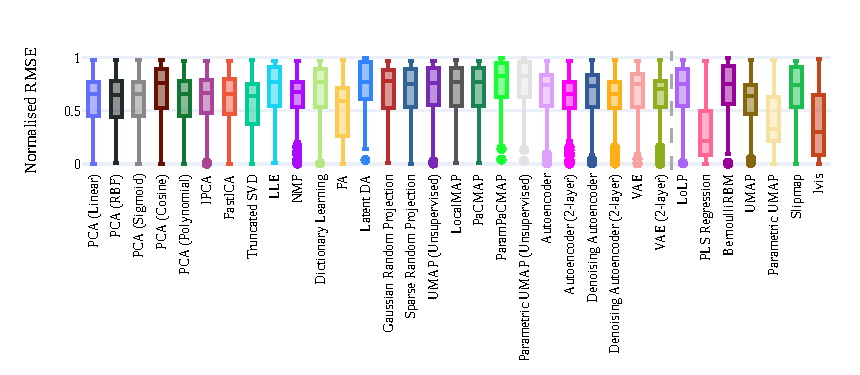
\includegraphics[width=\textwidth]{figures/04/epm/real_agg_sample_red_dim_1000_5.pdf}
        \caption{$N = 100, k=5$}
    \end{subfigure}
    \begin{subfigure}[t]{0.24\textwidth}
        \centering
        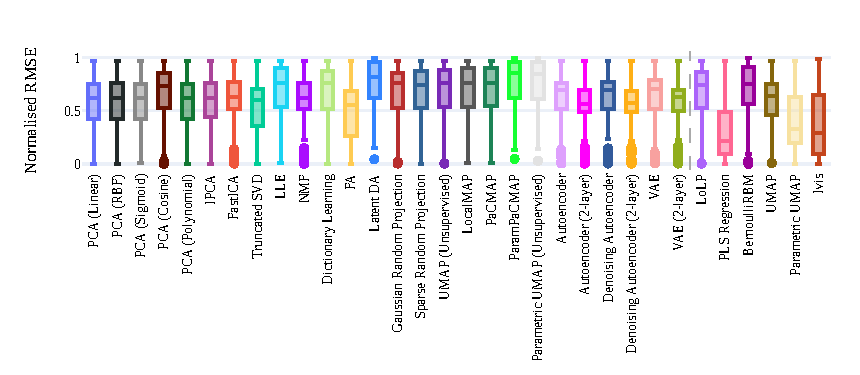
\includegraphics[width=\textwidth]{figures/04/epm/real_agg_sample_red_dim_1000_10.pdf}
        \caption{$N = 100, k=10$}
    \end{subfigure}
    \begin{subfigure}[t]{0.24\textwidth}
        \centering
        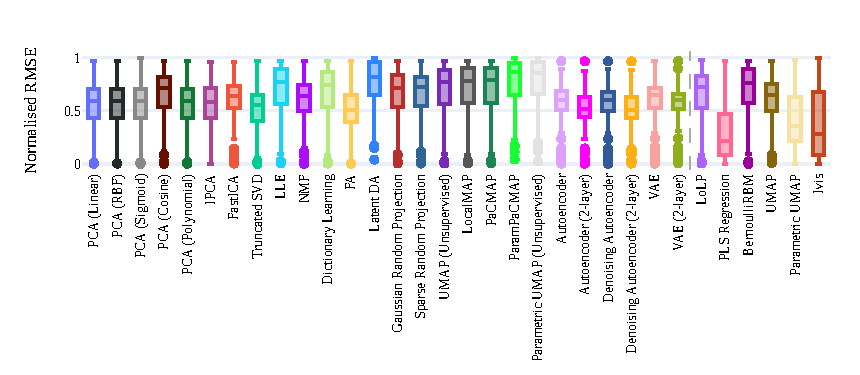
\includegraphics[width=\textwidth]{figures/04/epm/real_agg_sample_red_dim_1000_20.pdf}
        \caption{$N = 100, k=20$}
    \end{subfigure}
    \begin{subfigure}[t]{0.24\textwidth}
        \centering
        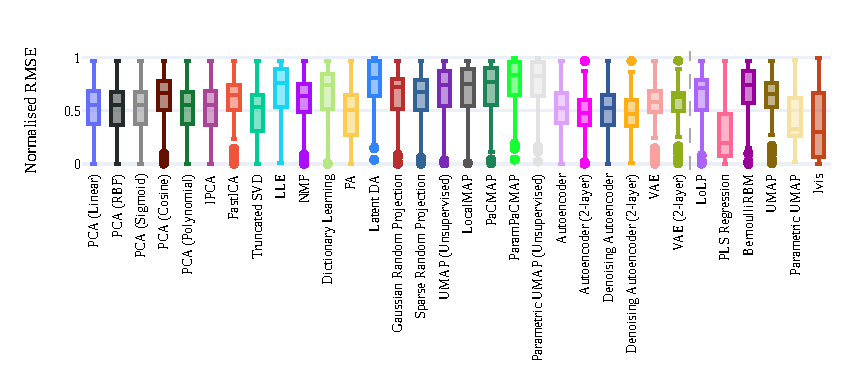
\includegraphics[width=\textwidth]{figures/04/epm/real_agg_sample_red_dim_1000_40.pdf}
        \caption{$N = 100, k=40$}
    \end{subfigure}
    \begin{subfigure}[t]{0.24\textwidth}
        \centering
        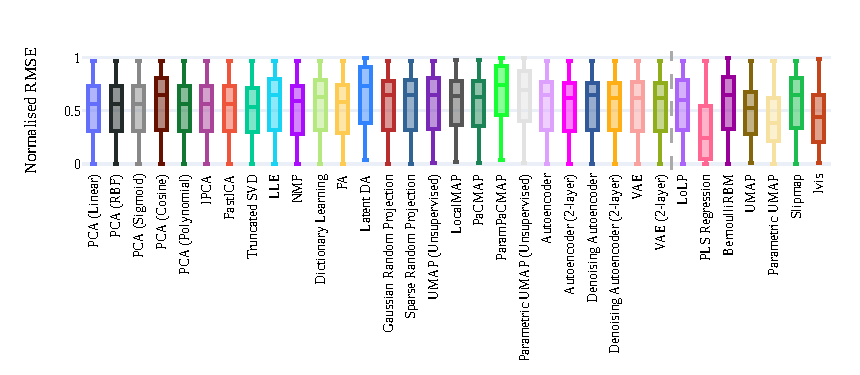
\includegraphics[width=\textwidth]{figures/04/epm/real_agg_sample_red_dim_100_5.pdf}
        \caption{$k = 5, N = 100$}
    \end{subfigure}
    \begin{subfigure}[t]{0.24\textwidth}
        \centering
        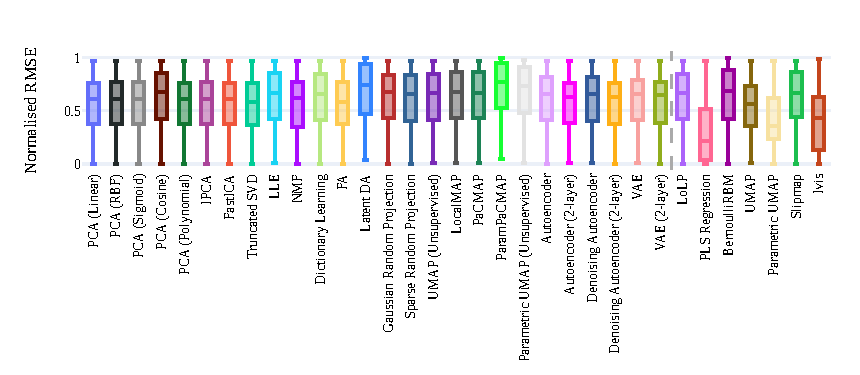
\includegraphics[width=\textwidth]{figures/04/epm/real_agg_sample_red_dim_200_5.pdf}
        \caption{$k = 5, N = 200$}
    \end{subfigure}
    \begin{subfigure}[t]{0.24\textwidth}
        \centering
        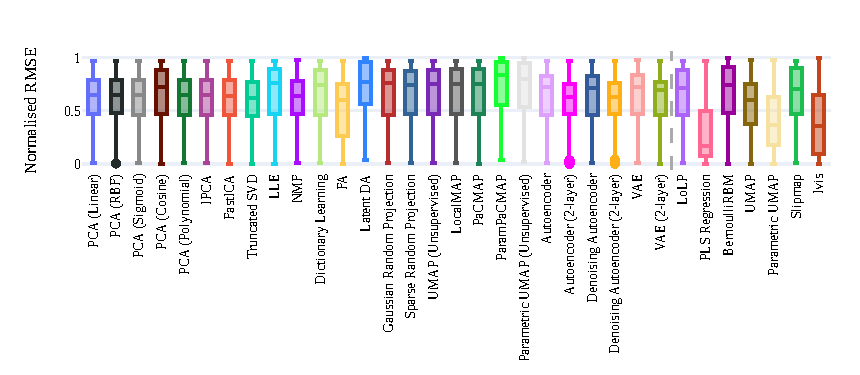
\includegraphics[width=\textwidth]{figures/04/epm/real_agg_sample_red_dim_500_5.pdf}
        \caption{$k = 5, N = 500$}
    \end{subfigure}
    \begin{subfigure}[t]{0.24\textwidth}
        \centering
        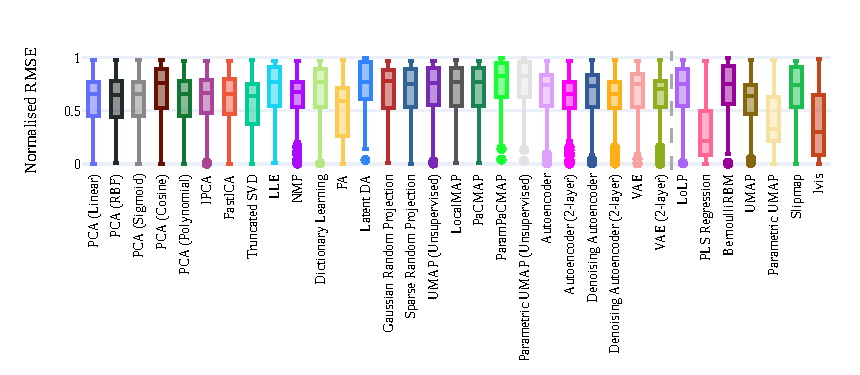
\includegraphics[width=\textwidth]{figures/04/epm/real_agg_sample_red_dim_1000_5.pdf}
        \caption{$k = 5, N = 1000$}
    \end{subfigure}





    \caption[Target function approximation on BBO task 1 for low- and high-dimensional benchmarks]{

    Performance of different dimensionality reduction methods aggregated across real-world benchmark problems in two settings: (a-d) for different target dimensionalities $k$ with initial sample size $N = 100$, and (e-h) for different initial sample sizes $N$ with target dimensionality $k = 5$, in terms of min-max normalised mean \gls{rmse} on \textbf{black-box optimisation task 1: target function approximation}; lower is better.
    Note that the input dimensionality is determined by the benchmark and cannot be controlled.
    PLS regression outperforms other methods across all target dimensionalities even when the initial sample size is small.




    }
    \label{fig:ch04:res-bbo-task1_real}
\end{figure}

So far, our assessment has focused on synthetic benchmarks for black-box optimisation. \cref{fig:ch04:res-bbo-task1_real} shows the results on real-world benchmarks. Figures (a–d) illustrate performance across varying target dimensionalities, with the initial sample size fixed at $N = 100$ (note that input dimensionality is determined by the benchmark and cannot be controlled). Across all target dimensionalities, PLS regression consistently outperforms other methods, reflecting its ability to extract components that are directly predictive of the target variables.
Figures (e–g) show the effect of varying the initial sample size while keeping the target dimensionality fixed at $k = 5$. Similar to the synthetic experiments, performance is relatively comparable across methods at smaller initial sample sizes, likely because most real-world benchmarks are high-dimensional, and small initial sample sizes limit the ability of the methods to extract reliable components. At an initial sample size of $N = 1000$, however, PLS regression clearly emerges as the best-performing method, confirming that adequate initial sample size is crucial for its predictive advantage in real-world, high-dimensional tasks.


\subsubsection*{Black-box optimisation task 2: Optimiser performance}

We now focus on the results of black-box optimisation task 2, where Bayesian optimisation is assisted by the dimensionality reduction methods. As in the previous task, we vary the target dimensionality $k$, while fixing both the initial sample size to $N = 100$ and the original input dimensionality to $D = 120$. The aggregated results across all synthetic benchmark problems are shown in \cref{fig:ch04:res-bbo-task2_red_dim}.
In contrast to the previous black-box optimisation task, PCA (RBF) consistently exhibits best performance across all target dimensionalities. Interestingly, PCA (Cosine) shows a noticeable improvement compared to its performance in the previous task, although it still falls short of PCA (RBF).

In contrast to relatively good performance of LLE in the machine learning task 1 (clustering ability), it is consistently the worst performing method in this task, closely followed by Bernoulli RBM for the highest target dimensionality.



\begin{figure}
    \centering
    \begin{subfigure}[t]{0.24\textwidth}
        \centering
        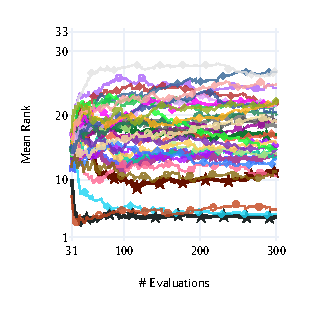
\includegraphics[width=\textwidth]{figures/04/bop/rank_100_120_5.pdf}
        \caption{$k=5$}
    \end{subfigure}
    \begin{subfigure}[t]{0.24\textwidth}
        \centering
        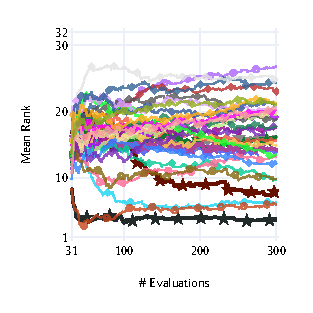
\includegraphics[width=\textwidth]{figures/04/bop/rank_100_120_10.pdf}
        \caption{$k=10$}
    \end{subfigure}
    \begin{subfigure}[t]{0.24\textwidth}
        \centering
        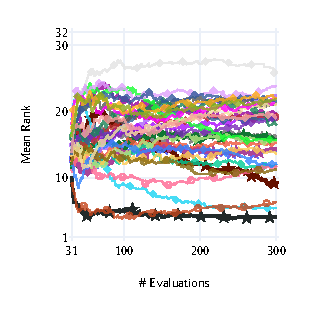
\includegraphics[width=\textwidth]{figures/04/bop/rank_100_120_20.pdf}
        \caption{$k=20$}
    \end{subfigure}
    \begin{subfigure}[t]{0.24\textwidth}
        \centering
        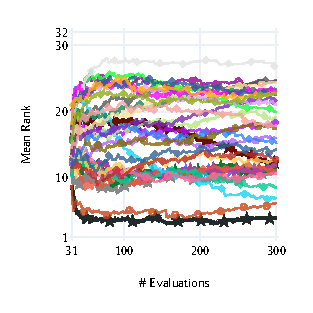
\includegraphics[width=\textwidth]{figures/04/bop/rank_100_120_40.pdf}
        \caption{$k=40$}
    \end{subfigure}
    \begin{subfigure}[t]{0.8\textwidth}
        \centering
        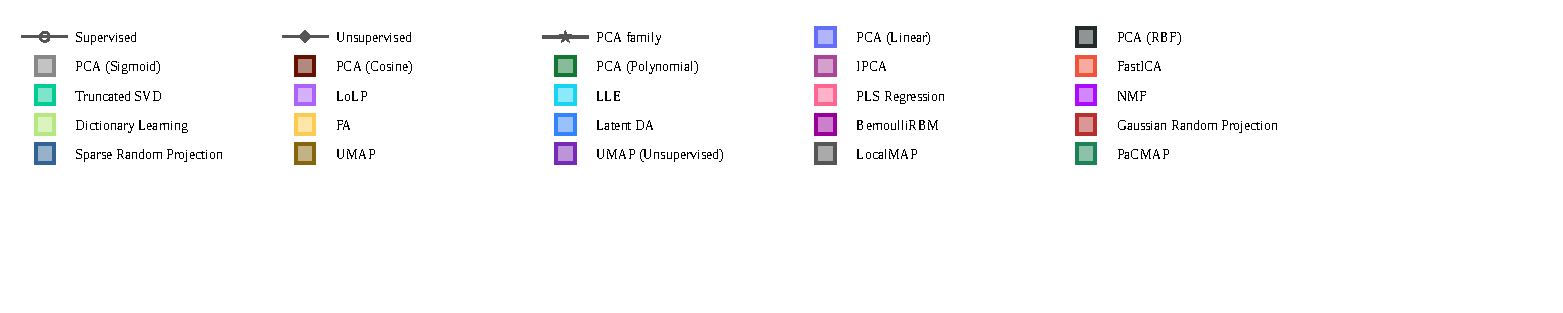
\includegraphics[width=1.0\textwidth,trim={1.5cm 4cm 3.7cm 0.0cm},clip]{figures/04/legend.pdf}
    \end{subfigure}
    \caption[Optimiser performance ranks on BBO task 2]{

    Performance of different dimensionality reduction methods aggregated across synthetic benchmark problems for different target dimensionalities $k$ with input dimensionality $D = 120$ and initial sample size $N = 100$, in terms of mean rank trajectories over the optimisation process on \textbf{black-box optimisation task 2: optimiser performance}; lower rank is better. 
    PCA (RBF) strongly outperforms all other methods across all target dimensionalities, followed by PLS regression and PCA (Cosine) for low target dimensionalities.
    LLE is the worst performing method, followed by Bernoulli RBM in the highest target dimensionality.


    }
    \label{fig:ch04:res-bbo-task2_red_dim}
\end{figure}

Next, we analyse the effect of varying input dimensionalities $D$ while fixing the initial sample size at $N = 100$ and the target dimensionality at $k = 20$.~\cref{fig:ch04:res-bbo-task2_diff_dims} shows the results aggregated across all synthetic benchmark problems. Across all input dimensionalities, PCA (RBF) consistently outperforms the other methods, confirming its robustness in this task.
Interestingly, unlike in black-box optimisation task 1 (target function approximation, which can also be seen as performance prediction from the point of view of empirical performance models~\citep{HutEtAl14}), where PLS regression excelled at lower input dimensionalities, here it performs better on higher-dimensional inputs on average. This shift likely reflects the difference in task objectives: in Bayesian optimisation, capturing broader input-space structure becomes more important as dimensionality increases, allowing PLS regression to extract useful predictive directions even without low-dimensional constraints.
Additionally, PCA (Cosine) shows improved performance across all input dimensionalities compared to the previous task, though it still remains slightly below PCA (RBF), suggesting that kernel-based PCA variants generally benefit more from the unsupervised optimisation setting.

Last, LLE exhibits consistent poor performance, in line with the previous findings for this task.


\begin{figure}
    \begin{subfigure}[t]{0.32\textwidth}
        \centering
        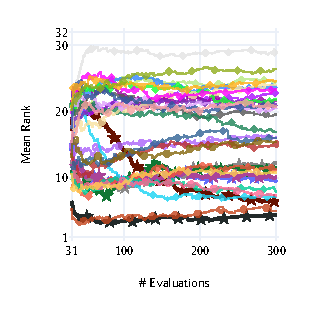
\includegraphics[width=\textwidth]{figures/04/bop/rank_100_40_20.pdf}
        \caption{$D=40$}
    \end{subfigure}
    \begin{subfigure}[t]{0.32\textwidth}
        \centering
        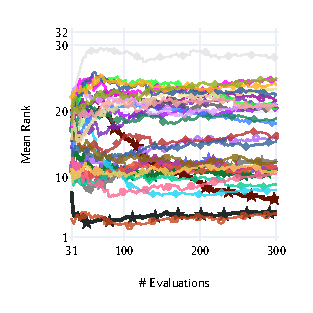
\includegraphics[width=\textwidth]{figures/04/bop/rank_100_60_20.pdf}
        \caption{$D=60$}
    \end{subfigure}
    \begin{subfigure}[t]{0.32\textwidth}
        \centering
        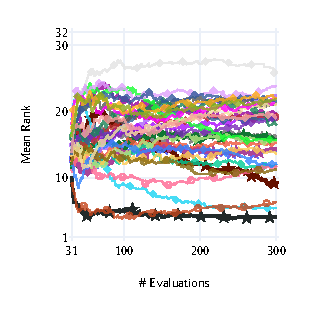
\includegraphics[width=\textwidth]{figures/04/bop/rank_100_120_20.pdf}
        \caption{$D=120$}
    \end{subfigure}
    \begin{subfigure}[t]{0.32\textwidth}
        \centering
        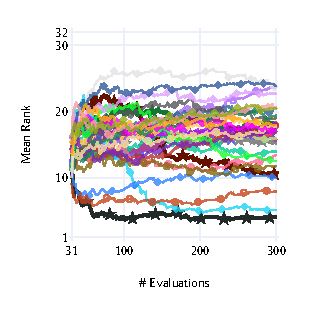
\includegraphics[width=\textwidth]{figures/04/bop/rank_100_240_20.pdf}
        \caption{$D=240$}
    \end{subfigure}
    \begin{subfigure}[t]{0.32\textwidth}
        \centering
        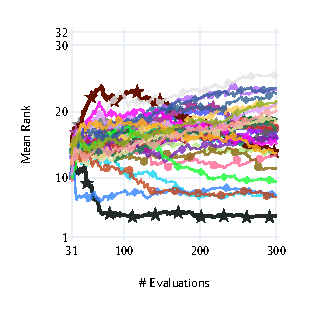
\includegraphics[width=\textwidth]{figures/04/bop/rank_100_500_20.pdf}
        \caption{$D=500$}
    \end{subfigure}
    \begin{subfigure}[t]{0.32\textwidth}
        \centering
        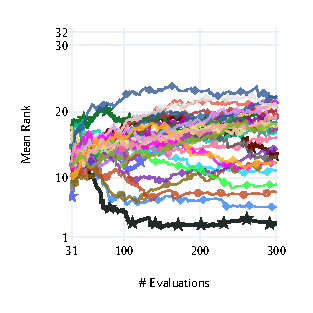
\includegraphics[width=\textwidth]{figures/04/bop/rank_100_1000_20.pdf}
        \caption{$D=1000$}
    \end{subfigure}
    \hspace{0.2cm}
    \begin{subfigure}[t]{0.8\textwidth}
        \centering
        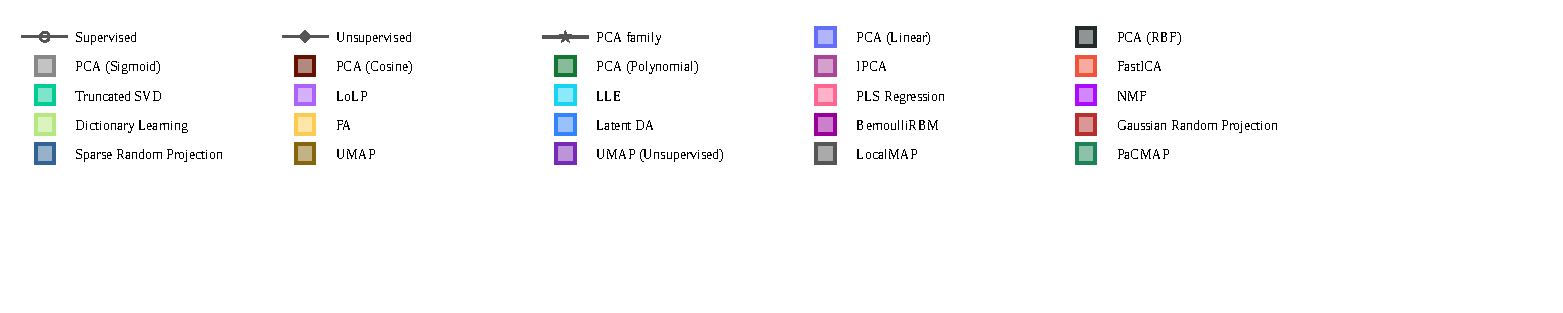
\includegraphics[width=1.0\textwidth,trim={1.5cm 4cm 3.7cm 0.0cm},clip]{figures/04/legend.pdf}
    \end{subfigure}
    \caption[Optimiser performance ranks on BBO task 2 by dimensionality]{

    Performance of different dimensionality reduction methods aggregated across synthetic benchmark problems for different input dimensionalities $D$ with target dimensionality $k = 20$ and initial sample size $N = 100$, in terms of mean rank trajectories over the optimisation process on \textbf{black-box optimisation task 2: optimiser performance}; lower rank is better. 
    PCA (RBF) strongly dominates all other methods across all input dimensionalities, followed by PLS regression for high input dimensionalities.
    PCA (Cosine) rapidly catches up with the top-ranked methods for lower-dimensional inputs, outranking PLS regression for $D = 240$ in the last stage of the optimisation process, but still consistently failing to outperform PCA (RBF).
    LLE is the worst performing method, followed by dictionary learning and Bernoulli RBM for lower input dimensionalities.


    }
    \label{fig:ch04:res-bbo-task2_diff_dims}
\end{figure}

We further examine the effect of varying initial sample sizes $N$ on performance, as shown in \cref{fig:ch04:res-bbo-task2_samples}. Figures (a–d) correspond to low-dimensional inputs ($D = 40$) with target dimensionality fixed at $k = 5$. In this setting, PCA (RBF) generally performs best, although PCA (Cosine) competes closely at small initial sample sizes, suggesting that with limited data, the choice of kernel can influence the stability of the projection.
Figures (e–h) show the results for high-dimensional inputs ($D = 1000$) with target dimensionality fixed at $k = 40$. Here, PLS regression performs comparably to PCA (RBF) when the initial sample size is large, indicating that with sufficient data, supervised methods can extract predictive directions even in very high-dimensional spaces, narrowing the gap with unsupervised methods.
\begin{figure}
    \centering
    \begin{subfigure}[t]{0.24\textwidth}
        \centering
        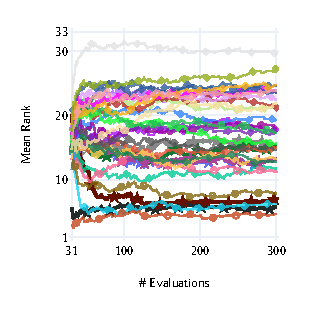
\includegraphics[width=\textwidth]{figures/04/bop/rank_100_40_5.pdf}
        \caption{\footnotesize$D = 40, k = 5, N = 100$}
    \end{subfigure}
    \begin{subfigure}[t]{0.24\textwidth}
        \centering
        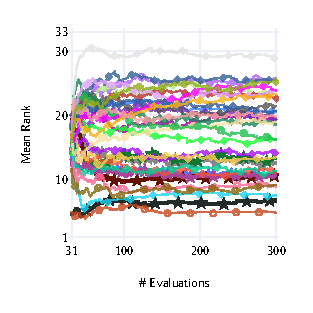
\includegraphics[width=\textwidth]{figures/04/bop/rank_200_40_5.pdf}
        \caption{\footnotesize$D = 40, k = 5, N = 200$}
    \end{subfigure}
    \begin{subfigure}[t]{0.24\textwidth}
        \centering
        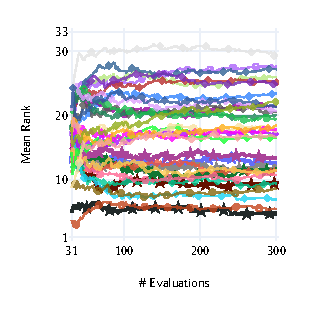
\includegraphics[width=\textwidth]{figures/04/bop/rank_500_40_5.pdf}
        \caption{\footnotesize$D = 40, k = 5, N = 500$}
    \end{subfigure}
    \begin{subfigure}[t]{0.24\textwidth}
        \centering
        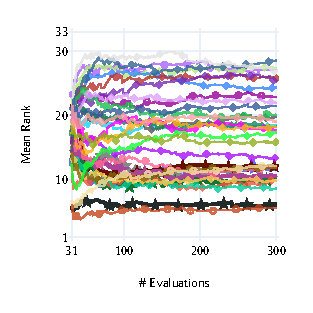
\includegraphics[width=\textwidth]{figures/04/bop/rank_1000_40_5.pdf}
        \caption{\footnotesize$D = 40, k = 5, N = 1000$}
    \end{subfigure}
    \begin{subfigure}[t]{0.24\textwidth}
        \centering
        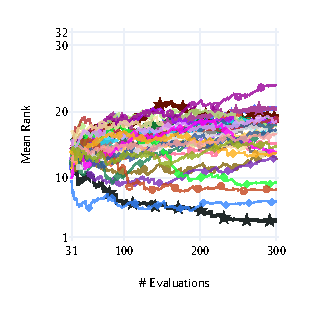
\includegraphics[width=\textwidth]{figures/04/bop/rank_100_1000_40.pdf}
        \caption{\footnotesize$D = 1000, k = 40, N = 100$}
    \end{subfigure}
    \begin{subfigure}[t]{0.24\textwidth}
        \centering
        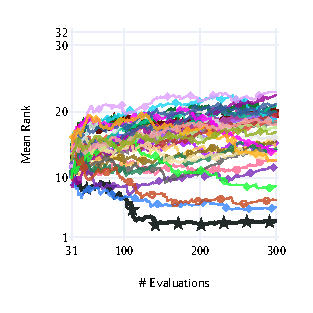
\includegraphics[width=\textwidth]{figures/04/bop/rank_200_1000_40.pdf}
        \caption{\footnotesize$D = 1000, k = 40, N = 200$}
    \end{subfigure}
    \begin{subfigure}[t]{0.24\textwidth}
        \centering
        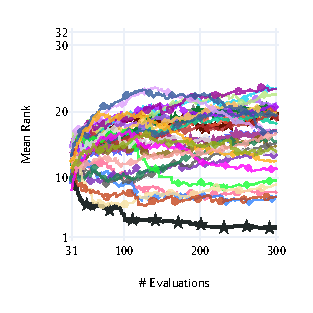
\includegraphics[width=\textwidth]{figures/04/bop/rank_500_1000_40.pdf}
        \caption{\footnotesize$D = 1000, k = 40, N = 500$}
    \end{subfigure}
    \begin{subfigure}[t]{0.24\textwidth}
        \centering
        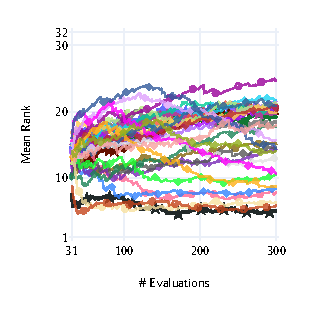
\includegraphics[width=\textwidth]{figures/04/bop/rank_1000_1000_40.pdf}
        \caption{\footnotesize$D = 1000, k = 40, N = 1000$}
    \end{subfigure}
    \hspace{0.2cm}
    \begin{subfigure}[t]{0.8\textwidth}
        \centering
        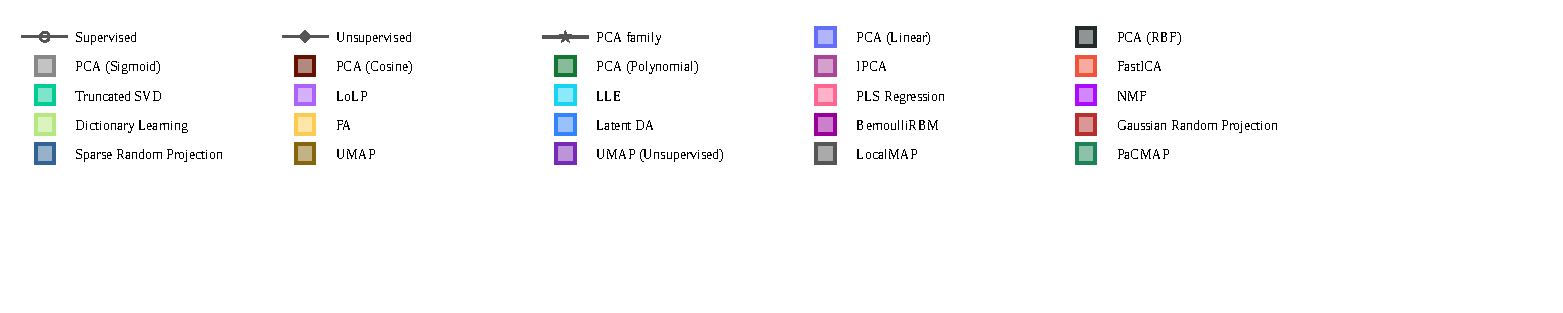
\includegraphics[width=1.0\textwidth,trim={1.5cm 4cm 3.7cm 0.0cm},clip]{figures/04/legend.pdf}
    \end{subfigure}
    \caption[Optimiser performance ranks on BBO task 2 for low- and high-dimensional benchmarks]{

    Performance of different dimensionality reduction methods aggregated across synthetic benchmark problems for different initial sample sizes $N$ in two settings: (a-d) with input dimensionality $D = 40$ and target dimensionality $k = 5$, and (e-h) with input dimensionality $D = 1000$ and target dimensionality $k = 40$, in terms of mean rank trajectories over the optimisation process on \textbf{black-box optimisation task 2: optimiser performance}; lower rank is better.
    PCA (RBF) is the top-ranked method across both settings, while PLS regression exhibits stronger performance for high-dimensional inputs than for low-dimensional ones.
    Dictionary learning, LLE, Bernoulli RBM and PCA (Cosine) are among the worst performers for low-dimensional inputs, whereas for high input dimensionalities, LLE stands out with its poor performance when the initial sample size is low, but quickly becomes indistinguishable from, \emph{e.g.,}, Bernoulli RBM (and other methods) as the initial sample size increases.


    }
    \label{fig:ch04:res-bbo-task2_samples}
\end{figure}


Finally, we look into the results on real-world benchmark problems in~\cref{fig:ch04:res-bbo-task2-real-world}, which paint a considerably different picture than synthetic benchmarks.
In Figures (a-d) we investigate the impact of varying target dimensionality $k$ while keeping the initial sample size fixed at $N = 100$. 
Unlike synthetic benchmarks where higher value of target dimensionality allowed for a relatively consistent performance improvement, here we see more complex optimisation dynamics, with highly variable performance across methods.
At the lowest target dimensionality we observe the most diverse performance of all methods, and the rapid convergence followed by plateaus suggests that most of the intrinsic information in dimension $5$ is captured early on in the optimisation process.
When target dimensionality is increased from $k = 20$ to $k = 40$, performance does not drastically improve, even though the advantage of methods that exhibited good performance for low values of $k$ diminishes.
This suggests that real-world optimisation problems may have intrinsic dimensionality in the range of $10$ to $20$ dimensions that are effectively exploitable (even with a small initial sample size of $100$), while additional target dimensions yield limited benefit and can even make the optimisation process more challenging.
Notably, for different target dimensionalities we cannot distinguish a clear winner among dimensionality reduction methods, while LLE is especially ill-suited for higher values of $k$ on this task.

Last, we assess the impact of varying initial sample sizes $N$ while keeping the target dimensionality fixed at $k = 5$ in Figures (e-h). 
Most methods start off with strong fluctuations in their convergence curves at the smallest initial sample size, suggesting that an insufficient amount of training data leads to unreliable dimensionality reduction mapping.
As the initial sample size increases, the convergence curves become smoother and more regular, and the performance gap between two distinct sets of methods becomes apparent.
Among good performers, we find in particular all PCA variants (with a notable exception of PCA (Cosine)), and PLS regression (which is top-ranked for the initial sample size of $N = 200$, and showed a consistent strong performance in the previous black-box optimisation task, as well as in this task on synthetic benchmarks).
Poor performance was yielded by LLE, Bernoulli RBM, LoLP, Gaussian and sparse random projections, dictionary learning, and, surprisingly, PCA (Cosine), which was often among the three top-ranked dimensionality reduction methods on synthetic benchmarks in this task.
The results indicate that the initial sample size used for training dimensionality reduction methods critically affects both optimisation quality and smoothness of convergence in real-world scenarios.
Moreover, as real-world function evaluations are expensive, this highlights a trade-off in allocating evaluations for training dimensionality reduction methods and for running the optimiser itself.

Overall, stark differences between performances of the methods on synthetic vs. real-world benchmarks likely reflect the heterogeneous nature of real-world problems, where features defining the search space often come from various domains and have complex interactions.
Across almost all considered settings, there is an evident tendency for methods to plateau well before the full optimisation budget is exhausted, causing the performance to stagnate.
This might indicate that, on real-world problems, the optimiser assisted by dimensionality reduction can effectively exploit only the global structure preserved in the reduced space, but loses access to more fine-grained details of these complex landscapes.
Finally, through high variability of observed behaviours across all settings, we see a general pattern of performance complementarity of different dimensionality reduction methods; while some methods excel on some problems, they perform poorly on others. 






\begin{figure}
    \centering
    \begin{subfigure}[t]{0.24\textwidth}
        \centering
        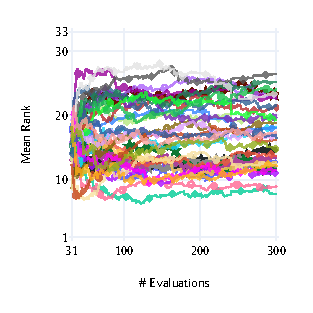
\includegraphics[width=\textwidth]{figures/04/bop/rank_real_100_5.pdf}
        \caption{$N = 100, k = 5$}
    \end{subfigure}
    \begin{subfigure}[t]{0.24\textwidth}
        \centering
        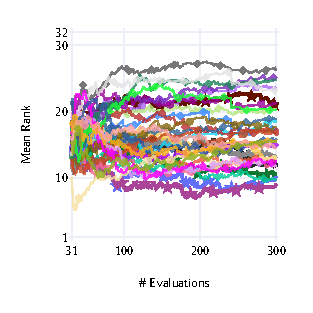
\includegraphics[width=\textwidth]{figures/04/bop/rank_real_100_10.pdf}
        \caption{$N = 100, k = 10$}
    \end{subfigure}
    \begin{subfigure}[t]{0.24\textwidth}
        \centering
        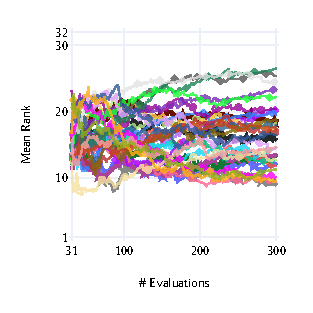
\includegraphics[width=\textwidth]{figures/04/bop/rank_real_100_20.pdf}
        \caption{$N = 100, k = 20$}
    \end{subfigure}
    \begin{subfigure}[t]{0.24\textwidth}
        \centering
        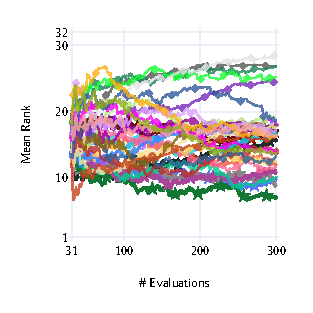
\includegraphics[width=\textwidth]{figures/04/bop/rank_real_100_40.pdf}
        \caption{$N = 100, k = 40$}
    \end{subfigure}
    \begin{subfigure}[t]{0.24\textwidth}
        \centering
        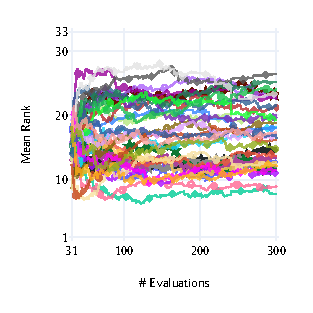
\includegraphics[width=\textwidth]{figures/04/bop/rank_real_100_5.pdf}
        \caption{$k = 5, N = 100$}
    \end{subfigure}
    \begin{subfigure}[t]{0.24\textwidth}
        \centering
        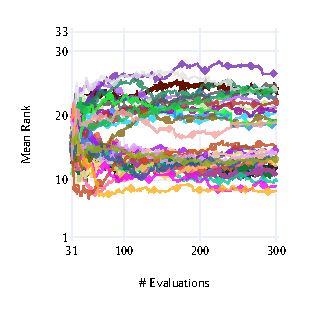
\includegraphics[width=\textwidth]{figures/04/bop/rank_real_200_5.pdf}
        \caption{$k = 5, N = 200$}
    \end{subfigure}
    \begin{subfigure}[t]{0.24\textwidth}
        \centering
        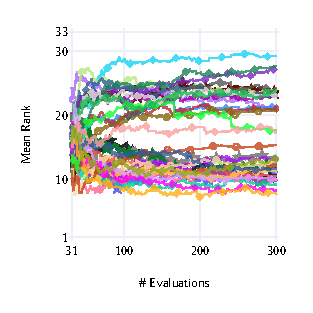
\includegraphics[width=\textwidth]{figures/04/bop/rank_real_500_5.pdf}
        \caption{$k = 5, N = 500$}
    \end{subfigure}
    \begin{subfigure}[t]{0.24\textwidth}
        \centering
        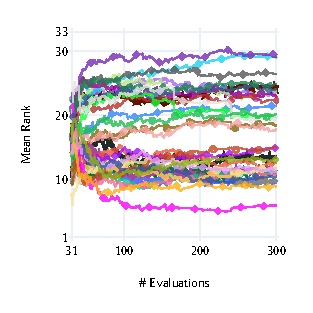
\includegraphics[width=\textwidth]{figures/04/bop/rank_real_1000_5.pdf}
        \caption{$k = 5, N = 1000$}
    \end{subfigure}
    \hspace{0.2cm}
    \begin{subfigure}[t]{0.8\textwidth}
        \centering
        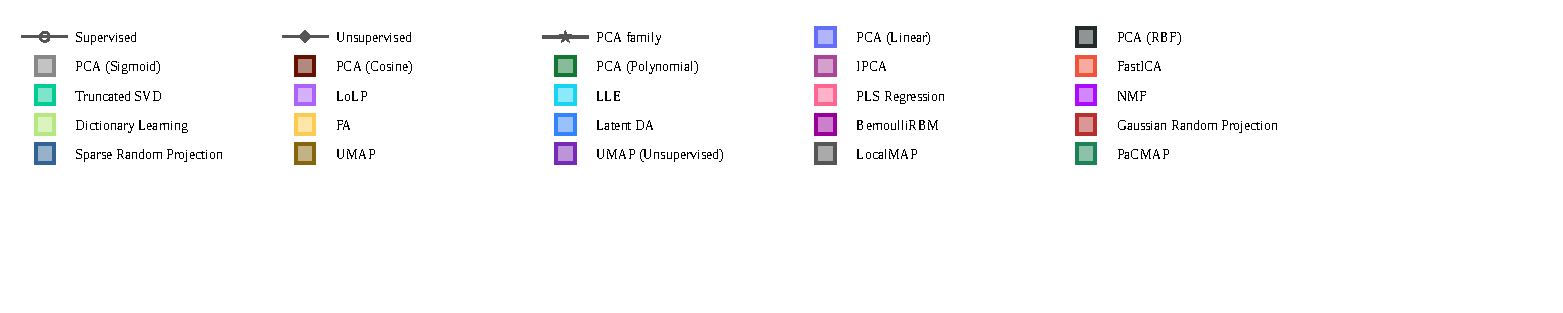
\includegraphics[width=1.0\textwidth,trim={1.5cm 4cm 3.7cm 0.0cm},clip]{figures/04/legend.pdf}
    \end{subfigure}
    \caption[Optimiser performance ranks on BBO task 2 for real-world benchmarks]{

    Performance of different dimensionality reduction methods aggregated across real-world benchmark problems in two settings: (a-d) for different target dimensionalities $k$ with initial sample size $N = 100$, and (e-h) for different initial sample sizes $N$ with target dimensionality $k = 5$, in terms of mean rank trajectories over the optimisation process on \textbf{black-box optimisation task 2: optimiser performance}; lower rank is better. Note that (i) the input dimensionality is determined by the benchmark and cannot be controlled, and (ii) figures (a) and (e) correspond to the same scenario.
    In the first setting, there is no single top-ranked method; LLE stands out as the worst performing method for higher target dimensionalities.
    In the second setting, as the number of initial samples grows, there appears a substantial spread in performance between two distinct sets of methods; notably, PCA (Cosine) is among the worst performers.


    }
    \label{fig:ch04:res-bbo-task2-real-world}
\end{figure}


\section{Running times}
\label{sec:ch04:rt}


In~\cref{fig:ch04:res-rt} we present the training and transformation running times of the dimensionality reduction methods for 2 selected OpenML datasets 

used in machine learning tasks 1 and 2: one with a lower dimensionality and a high number of elements, and one with a higher dimensionality and a low number of elements.

The running times are reported as CPU time.
We note that we report the transformation time 

needed for the two machine learning tasks,

but the times for black-box optimisation task 1 are similar 
as in this task we simply train and transform on a fixed dataset.

For black-box optimisation task 2, it is 

more challenging to isolate

the effect of the running time of the dimensionality reduction itself, as it is 

integrated in
the surrogate training and acquisition function optimisation, which are additional factors that can greatly affect the total running time.

We observe that for both training and transformation of low-dimensional datasets with a high number of elements (Figures (a-b)), LLE and PCA variants with non-linear kernels exhibit the highest running times.

For the high-dimensional dataset with a low number of elements (Figures (c-d)), the running times of those methods is lower compared to most other methods. In this setting, dictionary learning is the most expensive method in terms of running time.

We observe that Gaussian and sparse random projections consistently incur low running times, and that PLS regression is quite competitive in this regard for both datasets.



\begin{figure}
    \centering
    \begin{subfigure}[t]{0.24\textwidth}
        \centering
        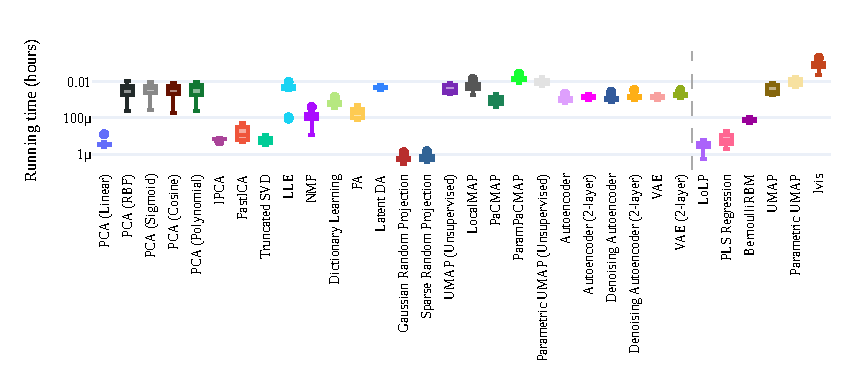
\includegraphics[width=\textwidth]{figures/04/time/9985_train_time.pdf}
        \caption{Training on dataset 9985}
    \end{subfigure}
    \begin{subfigure}[t]{0.24\textwidth}
        \centering
        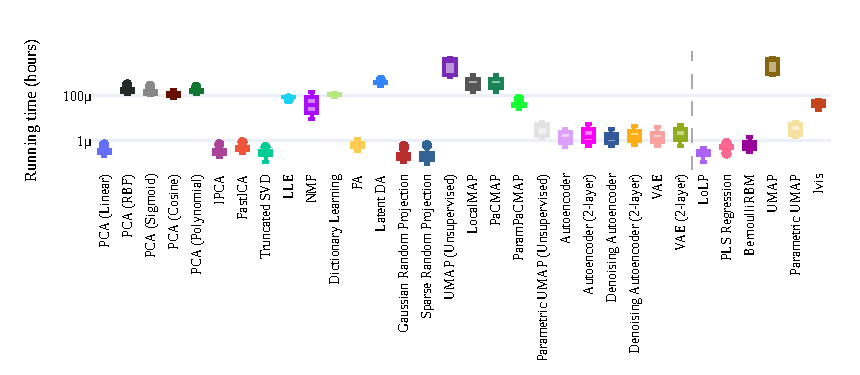
\includegraphics[width=\textwidth]{figures/04/time/9985_transform_time.pdf}
        \caption{Transform on dataset 9985}
    \end{subfigure}
        \begin{subfigure}[t]{0.24\textwidth}
        \centering
        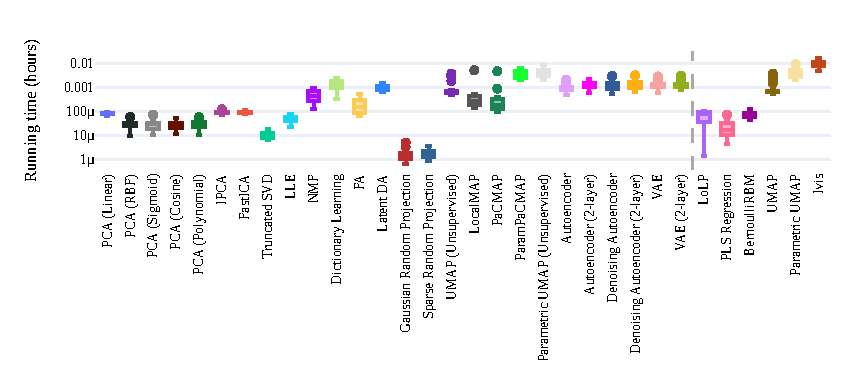
\includegraphics[width=\textwidth]{figures/04/time/9981_train_time.pdf}
        \caption{Train on dataset 9981}
    \end{subfigure}
    \begin{subfigure}[t]{0.24\textwidth}
        \centering
        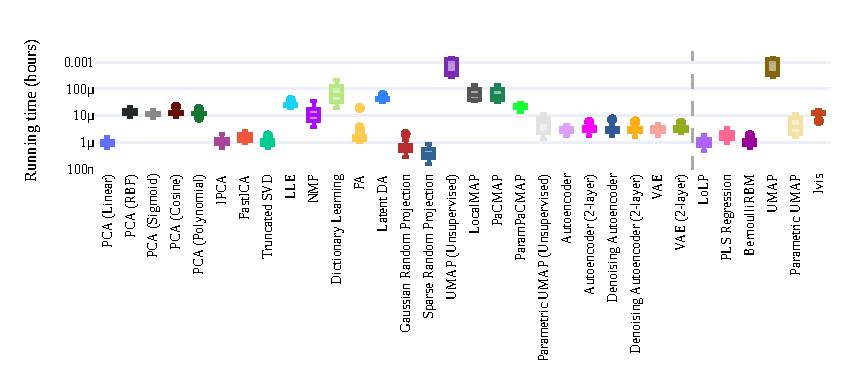
\includegraphics[width=\textwidth]{figures/04/time/9981_transform_time.pdf}
        \caption{Transform on dataset 9981}
    \end{subfigure}
    \caption[CPU hours for training and transformation]{

    Running times in terms of CPU hours for dimensionality reduction training (a, c) and transformation (b, d) of OpenML datasets 9985 (51 features and 6618 elements) and 9981 (856 features and 1080 elements).

    }
    \label{fig:ch04:res-rt}
\end{figure}



\section{Discussion}
\label{sec:ch04:disc}


Our comprehensive assessment of dimensionality reduction methods reveals fundamental differences in how the benchmarked methods perform in machine learning and black-box optimisation contexts.
An important insight of this study is the existence of strong task-dependent performance complementarity, as no single dimensionality reduction method dominates across all tasks.
This observation underscores that, to achieve best possible performance, proper method selection must be task-driven.

In the machine learning domain, we observed relatively similar performance of most dimensionality reduction methods.
For clustering, most methods struggled to preserve cluster homogeneity, indicating that class boundaries are challenging to capture, while cluster completeness was successfully retained by random projection methods and LLE in higher-dimensional subspaces.
In particular, good performance of LLE in this context may be due to its unsupervised nature and the fact it is designed to capture local structure.
Interestingly, this very characteristic of LLE might be responsible for its poor performance in assisting an optimiser.
For classification, most methods achieved a consistently high accuracy regardless of the underlying machine learning model (with the exception of random projections and Bernoulli RBM), suggesting that for well-structured tabular data, the choice of dimensionality reduction method has limited impact on downstream classification performance.
Both machine learning tasks showed that performance improves monotonically with target dimensionality, meaning that higher-dimensional projections retain more task-relevant information for structured datasets.

On the other hand, in the black-box optimisation domain, the choice of dimensionality reduction method had a substantial impact on the downstream performance, due to strong performance differences between methods.
For target function approximation, PLS regression was a top performer at lower target dimensionalities and moderate input dimensionalities, in line with the fact that it is a supervised method designed with the objective of extracting components directly predictive of function values.
However, for very-high dimensional inputs, or for insufficient data for training dimensionality reduction methods, PCA with the RBF kernel overtook PLS regression as the top-performing method.
A reason for this might be that unsupervised variance-based methods supported by an adequate non-linear kernel are able to capture essential problem structure when the original search space is extremely large and/or not well covered.


For optimiser performance, PCA with the RBF kernel excels by a large margin in assisting Bayesian optimisation in high-dimensional spaces.
This indicates that, in order to successfully perform Bayesian optimisation in the reduced space, dimensionality reduction has to be done via methods that preserve the global geometric structure of the objective function, and not merely predictive components.
For instance, LLE consistently performed worst in this task, showing that preserving local (instead of global) structure is detrimental for assisting optimisation procedures.


In particular, PLS regression (which was top-ranked for target function approximation) is not able to outperform PCA with the RBF kernel here.
Intuitively, this is because accurate prediction of function values does not necessarily translate to effective (and efficient) optimisation, as already observed in~\citep{FeuEtAl18b}.
In other words, problem characteristics required for guiding the search process fundamentally differ from those allowing for accurate function value regression, and the strong performance of PCA with the RBF kernel specifically suggests that capturing non-linear, distance-based relationships in the search space is crucial for optimisation, more so than explicit supervision on objective values.

We note that different sample sizes for training dimensionality reduction methods were used for the two black-box optimisation tasks.
However, as target function approximation via a surrogate model is a key component of Bayesian optimisation, we conjecture that some methods would tend to be effective in enhancing the optimiser, even if the surrogate (in the Bayesian optimisation loop of black-box optimisation task 2) is fitted on a smaller sample than for target function approximation of  black-box optimisation task 1.
We believe these observations to be of great importance for designing out-of-the-box robust Bayesian optimisation-based approaches to tackle high-dimensional real-world problems.















Taken together, these findings suggest that the task objective strongly shapes which dimensionality reduction method is most effective: supervised tasks favour methods aligned with predictive power, while unsupervised tasks benefit from methods that preserve geometric or topological structure.










\section{Chapter conclusion}
\label{sec:ch04:concl}



This chapter assessed the performance of a broad range of dimensionality reduction methods based on four carefully chosen downstream tasks from two different fields: machine learning and black-box optimisation.
Each task allows for empirically evaluating different aspects of dimensionality reduction methods, highlighting the task-dependent differences in their performance.
Specifically, we conducted a thorough benchmarking study of 16 dimensionality reduction methods 

(based on feature extraction) 
on these four tasks across a range of different settings (\emph{i.e.,} original dimensionality, target dimensionality, budget available for training dimensionality reduction methods), 

and derived practical insights into their suitability depending on their intended use.







In general, 

we observed that the choice of dimensionality reduction method depends on the task, as for each of the four tasks, different methods perform best. 

Moreover, even within the same task, different methods work best for different datasets or functions. 

While the performance differences are more prominent in  black-box optimisation tasks than in machine learning ones,

this shows that there is \textit{performance complementarity}~\cite{Rice76,FreEtAl16} between the dimensionality reduction methods, and that careful method selection is of key importance for achieving optimal performance.
In practice, dimensionality reduction methods are typically chosen based on good performance in similar scenarios.

We expect that meta-learning which method to use in which case can yield substantial performance gains and intend to further pursue research in this direction in future work.








Overall, dimensionality reduction methods often play a crucial role for solving problems in high-dimensional spaces. 
The results produced new insights into how these methods work in four broadly interesting scenarios, thus facilitating better understanding of their strengths and weaknesses.
These insights can be used in the future to help design new and improve existing dimensionality reduction methods for specific tasks.

\paragraph{Connection to the thesis}~
The results of this chapter show that there is no universally best representation: the usefulness of a reduced space depends on the downstream task and the structure of the problem.
This naturally leads to the question of how empirical performance prediction methods can adapt when different modelling choices are useful in different situations.
The next chapter addresses this question in Bayesian optimisation by dynamically combining complementary surrogate models.

\chapter{DyMBO: Dynamic Mixture of Surrogate Models for Hyperparameter Optimisation}\label{ch:ch05:dymbo}



\section{Introduction}
\label{sec:ch05:intro}
The performance of machine learning (ML) and deep learning (DL) models crucially depends on how their hyperparameters are tuned~\citep{LavDav06,BisEtAl23}.
Tuning the hyperparameters in order to achieve peak performance of the model on  a specific task is challenging even for experts. 
This process is often addressed through trial-and-error methods, requiring significant effort and resources.
Hyperparameter optimisation (HPO) techniques alleviate this burden by automatically searching for well-performing hyperparameter configurations, removing the need for human intervention~\citep{SnoEtAl12}.
While automated HPO techniques have shown great potential for classical ML models~\citep{SnoEtAl12,FeuEtAl22}, they are not as easily applicable to more complex ML and DL domains, where evaluating a single configuration of a model can be very expensive~\citep{BroEtAl20}.
Moreover, due to the lack of access to an explicit problem formulation, HPO is handled as a black-box problem.
Consequently, all automated HPO techniques rely on the only available information about the problem, \emph{i.e.}, evaluating the quality of candidate configurations, to steer the search towards the most promising regions of the search space and a good estimate of the global optimum.
% \changed{
Throughout this article, we consider HPO in the batched setting, in which $k$ candidate configurations are proposed and evaluated per BO iteration, as is standard practice in large-scale HPO~\citep{CowEtAl22,BisEtAl23}.
% }

Bayesian optimisation (BO)~\citep{Mockus12,Garnett23,Frazier18,Kushner62,Kushner64} is a surrogate-based, sample-efficient approach for global optimisation of expensive-to-evaluate black-box problems.
BO is particularly well-suited for settings with a very limited budget of available evaluations (relative to the size of the search space), such as HPO.
Various BO-based HPO techniques have been developed and successfully applied to this end; a prominent example is 
HEBO~\citep{CowEtAl22}, the winner of the NeurIPS BBO competition~\citep{TurEtAl20}.
One of the key components of BO is a 
% probabilistic \er{here, see comment below} 
\emph{surrogate model}, which is built on an initial sample of candidate solutions to approximate the objective function while also quantifying its uncertainty.
% \changed{
% In the sequential version of the BO algorithm, at each iteration 
At each iteration of BO, new candidate solutions are selected to be evaluated next by means of maximising an acquisition function defined on the surrogate.
% }
% At each iteration a new solution candidate is selected to be evaluated next by means of maximising an acquisition function defined on the surrogate.
The surrogate is then iteratively refined with newly observed candidate solutions, until the total budget of available evaluations has been exhausted.
% \er{I would be fine to revert it to the previous version, but then we need to say ``one or multiple solution candidates are selected"}
%
Fitting the surrogate model to the observed data is a prediction task that often involves probabilistic models. 
% \er{Since it \textit{often} involves probabilistic models, then I would remove the word ``probabilistic" above.}
BO then uses these probabilistic predictions of function values across the search space to guide the search towards a good estimate of the global optimum.
% \er{I'd start a new paragraph here and remove the ``thus", as this is the precise research challeng we address} 

% \changed{
The choice of the surrogate model strongly affects BO performance and is often linked to the dimensionality of the problem at hand and the nature of the corresponding search space.
% }
For continuous search spaces, Gaussian processes (GPs)~\citep{RasWil06} are the most widely adopted surrogate model and tend to be particularly effective in continuous search spaces~\citep{EggEtAl13,EggEtAl21,BenEtAl25}.
On the other hand, random forests (RFs)~\citep{Breiman01} as surrogate models natively support discrete and conditional search spaces, and tend to excel in higher problem dimensionalities, where GPs suffer from prohibitive computational complexity and reduced accuracy due to the increased volume of the search space
% search space volume
% \er{where GPs suffer from prohibitive computational complexity and reduced accuracy due to the increased search space volume}
~\citep{EggEtAl13,JenEtAl17,LiEtAl18}.
For complex HPO tasks in mixed domains, with numerical, ordinal and categorical hyperparameters, it is highly desirable to leverage the complementary strengths of inherently different surrogate models.
One natural way to achieve this is via ensemble methods, which have demonstrated their versatility in the context of BO-based HPO techniques for treating a wide range of heterogeneous problems~\citep{TurEtAl20,HofEtAl11}.
% \hh{the following didn't flow well and was rather unclear, so I've changed it a bit -- check carefully:}
% Here, we tackle complex HPO search spaces directly through adaptive choice of the most suitable surrogate model. 

% In conjunction with BO-based HPO techniques, multi-fidelity approaches~\citep{LiEtAl2017,LiEtAl20,FalEtAl2018,AwaEtAl21} have been widely used to address expensive HPO problems, due to the fact that they use cheap approximations of the target function at hand.
% \changed{
% However, they are not in scope of our work presented here, as they are conceptually different to the direction followed here, as they do not take into consideration the nature of the search space, but rather use low-fidelity evaluations as a proxy for full-fidelity evaluations to allow for the better use of the available budget.
% }
% \hh{I wonder about these last two arguments. Why should anyone care whether their working mechanisms differ if they address/solve the same problem? Which also begs the question why they would be out of scope ... perhaps it would be safer to say they are conceptually orthogonal to the direction followed here, as they do not take into consideration ..., but rather ... Then, a combination of our approach with multi-fidelity techniques could be an interesting direction for future work.}
% \todo{add references to multi-fidelity literature here and say it is out of scope of discussion for this paper}


\begin{figure}
    \centering
    % \includegraphics[width=\textwidth]{figs/Flowchart_ensemble-5.pdf}
    \resizebox{\textwidth}{!}{%
    \begin{tikzpicture}[
        >=stealth,
        myybox/.style={rectangle, rounded corners, draw=black, thick, fill=myyellow, align=center, text width=2.8cm, minimum height=1.8cm, font=\small\bfseries},
        myrbox/.style={rectangle, rounded corners, draw=black, thick, fill=mypink, align=center, text width=2.8cm, minimum height=1.8cm, font=\small\bfseries},
        mybbox/.style={rectangle, rounded corners, draw=black, thick, fill=mypurple, align=center, text width=2.6cm, minimum height=1.8cm, font=\small\bfseries},
        mydiamond/.style={diamond, draw=black, thick, fill=black, text=white, align=center, aspect=1.5, font=\small\bfseries, inner sep=2pt}
    ]
    
    % Group 1: Init
    \draw[fill=mygray, draw=mygray, rounded corners, thick] (-1.8, -2.2) rectangle (1.8, 2.2);
    \node[myybox, minimum height=1.4cm] (init1) at (0, 1.1) {Initial Design};
    \node[myrbox, minimum height=1.4cm] (init2) at (0, -1.1) {Weight\\Initialisation};
    
    % Group 2: Surrogate Model Fitting
    \draw[fill=mypinkbg, draw=mypinkbg, rounded corners, thick] (2.4, -1.6) rectangle (6.2, 2.5);
    \node[myybox, minimum height=2.0cm, text width=2.6cm] (surrn) at (4.7, 1.1) {};
    \node[myybox, minimum height=2.0cm, text width=2.6cm] (surr2) at (4.4, 0.6) {};
    \node[myybox, minimum height=2.0cm, text width=2.6cm] (surr1) at (4.1, 0.1) {Surrogate\\Model\\Fitting};
    \node[anchor=north east, font=\scriptsize] at ([shift={(-0.1,-0.1)}]surrn.north east) {Model $m$};
    \node[anchor=north east, font=\scriptsize] at ([shift={(-0.1,-0.1)}]surr2.north east) {Model 2};
    \node[anchor=north east, font=\scriptsize] at ([shift={(-0.1,-0.1)}]surr1.north east) {Model 1};
    
    \coordinate (c1) at (1.8, 0);
    \coordinate (c2) at (2.4, 0);
    \draw[->, thick] (c1) -- (c2);
    
    % Group 3: Model Ensemble
    \node[myrbox, text width=2.6cm] (ens) at (8.5, 0) {Model\\Ensemble/\\Selection};
    \draw[->, thick] (6.2, 0) -- (ens.west);
    
    % Group 4: AFO
    \node[myybox, text width=2.6cm] (afo) at (12.3, 0) {Acquisition\\Function\\Optimisation\\($k$ samples)};
    \draw[->, thick] (ens.east) -- (afo.west);
    
    % Group 5: Sample Eval
    \node[myybox, text width=2.6cm] (seval) at (16.1, 0) {Sample\\Evaluation\\and\\Optimum\\Update};
    \draw[->, thick] (afo.east) -- (seval.west);
    
    % Group 6: Accuracy Eval
    \node[myrbox, minimum height=2.0cm, text width=2.6cm] (accn) at (20.5, 1.1) {};
    \node[myrbox, minimum height=2.0cm, text width=2.6cm] (acc2) at (20.2, 0.6) {};
    \node[myrbox, minimum height=2.0cm, text width=2.6cm] (acc1) at (19.9, 0.1) {Accuracy\\Evaluation};
    \node[anchor=north east, font=\scriptsize] at ([shift={(-0.1,-0.1)}]accn.north east) {Model $m$};
    \node[anchor=north east, font=\scriptsize] at ([shift={(-0.1,-0.1)}]acc2.north east) {Model 2};
    \node[anchor=north east, font=\scriptsize] at ([shift={(-0.1,-0.1)}]acc1.north east) {Model 1};
    
    \draw[->, thick] (seval.east) -- (18.6, 0); 
    
    % Group 7: Model Weight Assign
    \node[myrbox, text width=2.6cm] (weight) at (24.3, 0) {Model Weight\\Assignment\\($w=1$ to best,\\$0$ otherwise)};
    \draw[->, thick] (21.7, 0) -- (weight.west); 
    
    % Group 8: EMA
    \node[myrbox, text width=2.6cm] (ema) at (28.1, 0) {Exponential\\Moving\\Average of\\model weights};
    \draw[->, thick] (weight.east) -- (ema.west);
    
    % Loop back from EMA top to Model Ensemble
    \draw[->, thick, dotted] (ema.north) -- ++(0, 2.0) -| (ens.north);
    
    % Budget Check logic
    \node[mydiamond] (budget) at (21, -4.5) {Budget\\exhausted?};
    \node[myybox, text width=2.6cm] (sampup) at (16.1, -4.5) {Sample Set\\Update with\\new samples};
    \node[mybbox] (ret) at (25.5, -4.5) {Return solution};
    
    \draw[->, thick] (ema.south) -- ++(0, -1.5) -| (budget.north);
    
    \draw[->, thick] (budget.west) -- node[above, font=\small\bfseries] {No} (sampup.east);
    \draw[->, thick] (budget.east) -- node[above, font=\small\bfseries] {Yes} (ret.west);
    
    \draw[->, thick] (sampup.west) -| (4.1, -1.6); 
    \end{tikzpicture}%
    }
    \caption{
    % \changed{
    Bayesian optimisation pipeline with dynamic ensembling and selection of surrogate models (\texttt{DyMBO}). In red, the blocks for the ensembling and selection strategy that have been plugged into the standard BO procedure. 
    % }
    We start by sampling an initial set of hyperparameter configurations and initialising the weights for surrogate models used to construct the ensemble. Within the BO loop, all surrogates are separately fitted to the past observations and then combined in the weighted ensemble, 
    which can be composed of only a single surrogate in case of greedy selection. The acquisition function is derived from the model ensemble and optimised to determine the next points to sample. The target function is evaluated on the points identified by optimising the acquisition function. The accuracy of the surrogate models is then evaluated on all sampled points, and surrogates are assigned new weights. Finally, the weighting scheme for the next iteration is obtained via an exponential moving average between the old and new weights, which is parametrised by a smoothing factor $\alpha$ in order to determine how much historical information is retained: 
    % \changed{
    the weighted ensemble is reconstructed if $\alpha < 1$ or the single most accurate surrogate is selected if $\alpha = 1$.
    % }. 
    % \todo{mark explicitly where sample evaluation is happening}
    }
    
    \label{fig:ch05:diagram}
\end{figure}

% \changed{
We propose a novel approach to enhance BO-based HPO performance by dynamically tailoring the surrogate model(s) during the optimisation process.
Our approach, dubbed \texttt{DyMBO}, dynamically adjusts the influence of multiple surrogate models used at each BO iteration, ranging from a weighted ensemble of complementary surrogates to a selection of a single best-performing surrogate.
To this end, \texttt{DyMBO}
assigns the largest weight to the surrogate model with the highest accuracy
on all observed points up to the current BO iteration and updates the 
weights via exponential moving average (see~\cref{fig:ch05:diagram} for details).
We use the term
% \hh{add: the term} 
\emph{ensemble} for the regime in which multiple surrogates retain non-zero weight, and \emph{selection} for the special case in which the weighting collapses to a single retained surrogate at each iteration.
% }

% \changed{
In particular, we present, for the first time, a dynamic tailoring approach to surrogate model combination and selection in the context of HPO. 
% }
This poses a significant challenge, as there is a trade-off between the time needed for finding the best hyperparameter configuration and the time complexity of target function evaluations (\emph{i.e.}, if the optimiser requires more time to determine the next configurations to sample, there is naturally less time available for evaluating the target function).
In the context of HPO, evaluating the target function means evaluating the performance of a given ML model for a given hyperparameter configuration on a given dataset.
Ensembling approaches in general require training and querying more than one surrogate model, which leads to more time required for the optimisation phase.
We assess the effectiveness of \texttt{DyMBO} %our dynamic surrogate ensembling 
on various HPO tasks involving numerous datasets and machine learning models. 
To this end, we compare \texttt{DyMBO} to several single-surrogate-based BO baselines and a range of competitive HPO frameworks, and we show that our method achieves a better average ranks than all other considered methods across both cheap and expensive functions in terms of time required for their evaluation. An overview of the results is shown in~\cref{fig:ch05:box_plot_mean_rank}.
We provide the code, instructions for reproducibility, as well as all figures in~\cref{sec:code-availability}. 

\begin{figure}
    \centering
    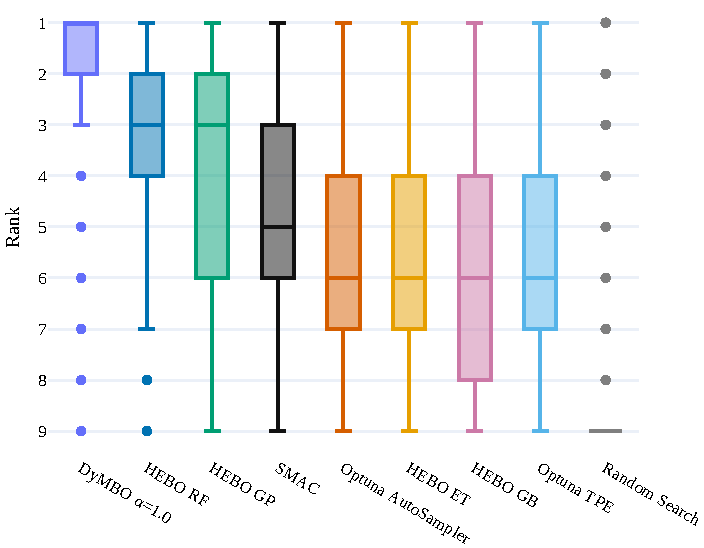
\includegraphics[width=0.5\linewidth]{figures/05/figs/figs/ranks/main_ranks_intro_box_plot_rank.pdf}
    \caption{
    % \changed{
    Box plot showing the ranks of various methods across 859 benchmark functions from YAHPO Gym and JAHS-Bench-201. \texttt{DyMBO} outperforms all baselines.
    % }
    }
    \label{fig:ch05:box_plot_mean_rank}
\end{figure}

The remainder of this paper is organised as follows: in~\cref{sec:ch05:back-rw}, we define the HPO problem, describe how BO operates, and position our approach with respect to related work on dynamically adapting BO components and using ensembles for enhancing BO performance.~\cref{sec:ch05:method} introduces 
% the \texttt{DyMBO} methodology.
our methodology for
% \changed{
dynamic ensembling and selection
% }
of surrogate models. 
In~\cref{sec:ch05:experiments}, we provide the technical details on the experimental setup and describe the benchmarks and baselines chosen for our empirical analysis. We present results and critically discuss them in~\cref{sec:ch05:res}. Finally, in~\cref{sec:ch05:concl-fw}, we provide concluding remarks and outline directions for future research.








\section{Background and related work}
\label{sec:ch05:back-rw}

In this section, we define the HPO problem and describe the working mechanisms of the BO framework. 
We also cover related work on dynamic design choices related to the components of BO, as well as using ensembles in BO.

\subsection{Hyperparameter optimisation} Let $\mathcal{A}$ be a learning algorithm with $n$ hyperparameters, $\Lambda_{i}$ the domain of the $i$-th hyperparameter, and $\mathbf{\Lambda} = \Lambda_{1} \times \Lambda_{2} \times \dots \Lambda_{n}$ the overall hyperparameter configuration space. 
We denote a hyperparameter configuration by $\mathbf{\lambda} \in \mathbf{\Lambda}$, and the algorithm $\mathcal{A}$ with its hyperparameters instantiated to $\mathbf{\lambda}$ by $\mathcal{A}_{\mathbf{\lambda}}$.
Given a dataset $D$, the objective of HPO is to find a hyperparameter configuration $\mathbf{\lambda}^{*}$ that minimises the loss $\mathcal{L}$ of a model fitted by algorithm $\mathcal{A}$ with hyperparameters $\mathbf{\lambda}$ on training data ${D}_{train}$, and evaluated on validation data ${D}_{validate}$, for a given loss function $\mathcal{L}$, \emph{i.e.},
\begin{equation}
\label{eq:ch05:def-hpo}
\mathbf{\lambda}^{*} \in \argmin_{\mathbf{\lambda} \in \mathbf{\Lambda}} 
\mathcal{L}(\mathcal{A}_{\mathbf{\lambda}}, {D}_{train}, {D}_{validate}) = \argmin_{\mathbf{\lambda} \in \mathbf{\Lambda}} c(\mathbf{\lambda})
\end{equation}
Here, $c(\mathbf{\lambda})$ is a shorthand for the loss function when $\mathcal{A}_{\mathbf{\lambda}}$ and $D$ are fixed.
Note that $c(\mathbf{\lambda})$ is a black-box function, without a closed-form expression nor analytic gradient information.

\subsection{Bayesian optimisation} 
\label{sec:ch05:bac_bo}

Bayesian optimisation (BO)~\citep{Mockus12,Garnett23,Frazier18,Kushner62,Kushner64} is a family of surrogate-based algorithms for efficient global optimisation of black-box problems.
Typically, BO consists of three main components: an \emph{initial design}, \emph{i.e.}, in HPO, a set of candidate hyperparameter configurations $\boldsymbol{\lambda} = (\lambda^{(1)},\ldots, \lambda^{(r)})$ and their evaluations 
$c(\boldsymbol{\lambda}) = (c(\lambda^{(1)}),\ldots, c(\lambda^{(r)}))$; a \emph{surrogate model} (fitted to the 
% initial 
observations) that returns an approximation $\hat{c}(\mathbf{\lambda})$ of the unknown loss function $c(\mathbf{\lambda})$ while capturing the uncertainty in the prediction $\hat{\sigma}(\mathbf{\lambda})$ on unobserved points in the search space; and an \emph{acquisition function}, which is optimised to suggest candidate solutions to be evaluated next, usually balancing exploration and exploitation of the search space.
BO then evaluates the most promising candidate solutions.
% \er{``interesting'' doesn't seem like a technical term. I would replace with ``promising'', ``valuable''...}
To approximate the expensive objective function, BO typically employs a Gaussian process (GP) model as the surrogate. The GP model defines a distribution over functions on the configuration space $c(\lambda)\sim\mathcal{GP}_c(\mu(\lambda),\text{cov}(\lambda,\lambda'))$, where 
$\mu(\cdot)$ 
is a mean function and 
$\text{cov}(\cdot,\cdot)$
is a covariance function. If we consider an observation model 
$y_i = c(\lambda^{(i)}) + \varepsilon_i$
with normally distributed noise, 
$\varepsilon_i\sim\mathcal{N}(0,\sigma^2_\varepsilon)$, 
the predicted value by the GP model at one unknown configuration 
$\lambda$ will also follow a normal distribution with mean 
$\mu(\lambda)=K_{\lambda,\boldsymbol{\lambda}}(K_{\boldsymbol{\lambda},\boldsymbol{\lambda}}+\sigma^2_\varepsilon I)^{-1}\boldsymbol{y}$ and variance $\sigma^2(\lambda)=\text{cov}(\lambda,\lambda)-K_{\lambda,\boldsymbol{\lambda}}(K_{\boldsymbol{\lambda},\boldsymbol{\lambda}}+\sigma^2_\varepsilon I)^{-1} K_{\boldsymbol{\lambda},\lambda}$, 
where $\boldsymbol{y}=(y_1,\ldots,y_r)$ is the vector of observations, $K_{\boldsymbol{\lambda},\boldsymbol{\lambda}}=[\text{cov}(\lambda^{(i)},\lambda^{(j)})]_{\lambda^{(i)},\lambda^{(j)}\in\boldsymbol{\lambda}}$ is the covariance matrix, and $K_{\lambda,\boldsymbol{\lambda}}=[\text{cov}(\lambda^{(i)},\lambda)]_{\lambda^{(i)}\in\boldsymbol{\lambda}}$ is the correlation vector for all samples.
% \aj{FIXED, please check: inconsistent use of bold for the lambda subscripts in the kernel K}
GPs as a surrogate model inherently provide both the mean and the variance vector.

However, GPs are not the only surrogate model used in BO. Another common choice for a surrogate model are tree-based models, 
such as random forests (RFs). 
Tree-based models traditionally predict only the mean of the given data (\emph{e.g.}, in a regression setting). 
In this case, the variance is defined based on the variance of the predictions of the leaves~\citep{HutEtAl11}. 
With $t(\lambda)$ being the prediction of a tree $t \in T$, we calculate the mean $\mu(\lambda)$ and variance $\sigma^2(\lambda)$ for a set of trees $T$ as follows:
% \hs{GB is now calculated as quantile regression}
\begin{equation}
    \mu(\lambda)=\frac{1}{|T|} \cdot \sum_{t\in T} t(\lambda) \; ,
\end{equation}
\begin{equation}
    \sigma^2(\lambda)=\frac{1}{|T|} \cdot \sum_{t\in T} (t(\lambda) - \mu(\lambda))^2 \; .
\end{equation}
% \changed{
% An exception is gradient boosting (GB), a tree-based model for which uncertainty is estimated via quantile regression~\citep{Koenker1978}.
% Here, two separate models are fitted to predict the upper and lower quantiles of the output distribution, and the variance is derived from the spread between these quantiles. This is done similarly to the implementation in the \textsc{scikit-optimize} package\footnote{\url{https://github.com/scikit-optimize/scikit-optimize}}.
% }
% \changed{
Alternatively, uncertainty can be estimated via quantile regression~\citep{KoeBas78}, using two separate models to predict the upper and lower quantile of the output distribution, and deriving variance from the spread between these quantiles.
We adopt this approach to estimate uncertainty for another tree-based model, gradient boosting (GB); this is done similarly to the implementation in the \textsc{scikit-optimize} package.\footnote{\url{https://github.com/scikit-optimize/scikit-optimize}}
% }
% \hh{this sounds as if the scikit-optimize implementation was the first to define GB ... surely not true?? please reword to properly reflect (a) the original concept of gradient boosting and (b) its implementation in the package. I'd also consider writing something like `Alternatively, uncertainty can be estimated as is done in gradient boosting, using two ... Footnote signs at the end of sentences follow the full stop.}

BO proceeds iteratively until a termination criterion is met. In each iteration, it optimises the acquisition function %to suggest high-potential solutions by
by repeatedly querying the surrogate model to generate a pool of candidate solutions. It then evaluates the most high-potential solutions (\emph{i.e.}, the solutions that maximise the acquisition function) from this pool,
refines the surrogate model based on the new observations, and updates the optimum if the new point improves upon the true function value of the best observation so far.
% \changed{
Throughout this work, we consider the batched setting, in which $k$ configurations are proposed and evaluated per BO iteration; see~\cref{sec:ch05:method}. This is reflected in the acquisition and update steps described here.
% }

Among the many variants of BO from the literature, in this work, we focus on the state-of-the-art method for HPO to empirically evaluate our method: HEBO~\citep{CowEtAl22}.
HEBO (Heteroscedastic and Evolutionary Bayesian optimisation) is a BO-based optimiser with several advancements 
% \changed{
targeting each of the core BO components described above.
For the surrogate model, HEBO uses GP with two key transformations: a power transformation applied to the output observations $\boldsymbol{y}$ and a Kumaraswamy transformation applied to the input configurations $\boldsymbol{\lambda}$; 
% \hh{minor change:}
jointly, these address heteroscedasticity in the noise $\epsilon$ and non-stationarity in the covariance matrix $K_{\boldsymbol{\lambda},\boldsymbol{\lambda}}$.
\citet{CowEtAl22} showed that these transformations enhance the ability of GPs to accurately approximate the mapping between configurations and corresponding performances, which is crucial for HPO.
% on performance data. 
% \er{``performance'' used twice with different meanings, could be confusing. What do we exactly mean with ``performance data'' and, earlier, with ``performance observations''? Is it another phrasing for solution quality, specific for HPO?}
For the acquisition function, rather than optimising a single criterion, HEBO samples new candidate configurations by maximising MACE~\citep{LyuEtAl18}, a multi-objective acquisition function that simultaneously considers expected improvement (EI)~\citep{Mockus75}, probability of improvement (PI)~\citep{Kushner64}, and upper confidence bound (UCB)~\citep{ForEtAl08}, providing a more robust balance between exploration and exploitation of the search space than any single acquisition function alone.
% \hh{modified:}
Additional details on HEBO can be found in~\cref{sec:imp_det}.

% \changed{
In conjunction with BO-based HPO techniques, \emph{multi-fidelity approaches}~\citep{LiEtAl18,LiEtAl20,FalEtAl18,AwaEtAl21} have been widely used to address expensive HPO problems, due to the fact that they use cheap approximations of the target function at hand.
However, these fall outside the scope of our work presented here, as they do not take into consideration the nature of the search space, but rather use low-fidelity evaluations as a proxy for full-fidelity evaluations to allow for the better use of the available budget; this constitutes a conceptually different approach from the one followed here.
% }
% }
% to improve performance. 
% \todo{connect the advancements of HEBO relative to the details of BO above to help understand where the gains of HEBO come from}
% It applies a power transformation to the performance data and 
% the Kumaraswamy transformation to the input data to tackle heteroscedasticity and non-stationarity. 






\subsection{Dynamic component selection in Bayesian optimisation}
As a modular framework, BO performance is highly sensitive to design choices of its modules. 
Different sampling strategies for the initial design, such as Latin hypercube sampling~\citep{McKEtAl00}, low-discrepancy sequences (\emph{e.g.}, Sobol~\citep{AntSal79}) or random uniform sampling; different surrogate models, such as GPs or RFs; and different acquisition functions, such as EI, PI or UCB -- all affect the overall BO performance to various degrees~\citep{BosEtAl20,LinEtAl19,CowEtAl22}. 
Despite few works showing the potential of automated selection of components~\citep{BenTom18,BenEtAl22,BenEtAl22}, the settings for each component are typically chosen by practitioners beforehand depending on the desired use-case, and are fixed for the entire optimisation procedure.

However, there have been efforts to show that the dynamic choices of BO modules lead to performance gains across multiple contexts.
Prior attempts to investigate the dynamic adjustment of acquisition functions include works on mixed acquisition function strategies, \emph{e.g.}, a self-adjusting approach to balance the exploration-exploitation trade-off~\citep{BenEtAl23}, an online multi-armed bandit strategy on a portfolio of acquisition functions~\citep{HofEtAl11}, or an online update of weights in a portfolio of acquisition functions~\citep{KanEtAl20}.
When it comes to dynamic adjustment of surrogate models, several directions have been investigated, notably an online selection of surrogate models based on their ranking in each BO iteration~\citep{BagEtAl16}, adaptive global surrogate modelling via genetic algorithm-driven sampling~\citep{GorEtAl09}, or adaptive combining of surrogates based on crowding distance trust regions~\citep{ZhaEtAl12}.
It has also been shown that dynamic component selection in general is beneficial in terms of performance in other related areas, \emph{e.g.}, in algorithm configuration~\citep{BieEtAl20}, evolutionary computation~\citep{KarEtAl15,DoeDoe20}, planning~\citep{SpeEtAl21}, and deep learning~\citep{AdrEtAl22}.

\subsection{Ensembles in Bayesian optimisation}
% \hs{clarify how we are different and novel}
% \changed{
Ensembles of ML models have been shown to outperform single models for a wide range of use-cases~\citep{SagRok18,OpiMac99,Rokach10,DonEtAl20}. 
Consequently, using ensembles in the context of BO is not a new idea.
% \changed{
Nevertheless, to the best of our knowledge, our work is the first one to use a 
% \hh{simplify: is the first to use a ...}
dynamic tailoring strategy, ranging from full ensembling to greedy selection, for surrogate models in mixed discrete-continuous search spaces of problems that tend to be very expensive to evaluate in practice, such as HPO.
% }
A series of earlier studies has demonstrated the advantage of using ensembles in BO, most notably in engineering~\citep{JiaEtAl20,ZhoEtAl11}; however, the search spaces explored in these are of a purely continuous nature.
Various ensembling strategies investigated in the literature do not apply in a straightforward manner to our use-case, \emph{e.g.}, optimal weighting strategies of surrogates trained on existing observations~\citep{HanEtAl22} or on extracted features~\citep{GuoEtAl19} have been designed for multi-objective constrained optimisation, while techniques for optimising multiple acquisition functions on multiple surrogates and combining them accordingly~\citep{HuaEtAl22, BeaEtAl19} have been developed for purely discrete search spaces.
Moreover, all these existing approaches consider a static (\emph{i.e.}, global) ensemble construction which is then used throughout the entire optimisation process. Additionally, ensembles of surrogate models are commonly used in meta-learning for BO~\citep{WisEtAl16,FeuEtAl22}. 
% \er{We use both BO and the full name, Bayesian optimization, in text. We should stick to BO once the acronym is introduced.}
% \aj{This is now fixed. We only use the full name ``Bayesian optimisation'' in the abstract, for the first time we introduce it in the manuscript, and then in section titles (because it is cleaner than using an acronym in the title, IMO, but we can change this), and in the Figure 1 caption, because it should be self-contained (but we can also change this). }
% \changed{
In contrast, our method operates in a dynamic fashion, tracking the accuracy of surrogates and adjusting the surrogate weighting on the fly.
% }

Dynamic model ensembles in BO have been used for time-series prediction~\citep{Liu23}, which constitutes a fundamentally different use-case. 
% \citet{Liu2020} have proposed a multi-fidelity approach by combining two GP %regression 
% models approximating both high- and low-fidelity data during the BO procedure, whereas our work considers a fully black-box setting. 
Dynamic ensembling has also been considered in a non-BO context, \emph{e.g.}, for neural decoding in brain-computer interfaces~\citep{QiEtAl19}.
% \hh{The next sentence needs to be modified, since it doesn't make an argument why these are incompatible (you could refer to what was stated earlier, of course).}
The fact that HPO problems can be expensive to evaluate and involve mixed discrete-continuous search spaces, with possibly many conditional hyperparameters, renders previous approaches hardly applicable in this context.
% The incompatibility of these works with the HPO use-case renders them non-applicable in our context.
Related approaches also substantially differ from our proposed methodology, as none of them considers the use of exponential moving averages to capture the history of model performance, nor a weighting scheme that is based on the accuracy on all past observations.
Furthermore, we consider ensembles of regression models from inherently different families.
% To the best of our knowledge, dynamic surrogate ensembles have so far not been applied in the context of HPO.
Thus, in relation to previous work, we not only consider a new use-case, but an entirely different challenge compared to other real-world applications, due to a key trade-off between the budget for evaluating the (possibly very expensive) target function and the budget for finding the optimal %hyperparameter 
configuration.
% }



\section{Methodology}
\label{sec:ch05:method}

% Our dynamic ensembling approach works as follows. 
% \changed{
Our method works as follows.
% }
The BO procedure is launched with an initial set of hyperparameter configurations. We initialise the weights and assign them to the models used to construct the ensemble. We denote the initial weight for the surrogate model $m$ as $w_{0,m}$. 
Then, the BO loop begins. At each iteration $t$, we train all surrogate models separately on all available samples accumulated up to that point and create a weighted ensemble. The weighted ensemble is a convex combination of the surrogate models, with coefficients defined as the normalised model weights of that iteration, \emph{i.e.},:
\begin{equation}
    \hat{w}_{t,m} = \frac{\bar{w}_{t,m}}{\sum_{j\in M}{\bar{w}_{t, j}}},
\end{equation}
where $M$ is the set of available surrogate models and $\bar{w}_{t,m}$ is the weight of model $m$ at iteration $t$. This way we make sure that $\sum_{m\in M} \hat{w}_{t,m} = 1$ with $0\leq \hat{w}_{t,m} \leq 1$.
The ensemble can then predict the $\mu_{\text{ens}}(\lambda)$ and $\sigma_{\text{ens}}(\lambda)$ of the performance for an unobserved configuration $\lambda$ by using a weighted average 
of the individual model predictions $\mu_m(\lambda)$ and their standard deviations $\sigma_m(\lambda)$:
\begin{equation}
    \mu_{\text{ens}}(\lambda)= \sum_{m\in M} \hat{w}_{t,m} \cdot \mu_{m}(\lambda),
    \label{ch05:ens_mu}
\end{equation}
\begin{equation}
    \sigma_{\text{ens}}(\lambda)= \sum_{m\in M} \hat{w}_{t,m} \cdot \sigma_{m}(\lambda).
    \label{ch05:ens_sigma}
\end{equation}

% \changed{
We note that~\cref{ch05:ens_sigma} combines the standard deviations $\sigma_{m}(\lambda)$ directly rather than the variances $\sigma_{m}^{2}(\lambda)$; we adopt this convention for consistency with the expected use of $\sigma_{ens}$ as a scale parameter in the acquisition function definition.
We discuss an alternative formulation based on the rule of total variance in~\cref{sec:ch05:ablations}.
% }
We also note that, in preliminary experiments, we investigated a variation of our ensembling method that applies different weighting schemes for the mean and the variance. However, this did not yield sufficient improvements to justify a more complex method definition. Further details can be found in~\cref{sec:ch05:ablations}.

% \hh{minor change in the following:}
% \changed{
\paragraph{Accuracy evaluation via ranking loss.}
In the next stages, at each iteration $t$, we optimise the acquisition function and select the candidates to be sampled, $\lambda_t^{(1)},\lambda_t^{(2)},\dots,\lambda_t^{{(k)}}$, as is typically done in BO. We then evaluate the accuracy of the different surrogate models using ranking loss (RL)~\citep{FeuEtAl22} on all sampled points. 
% \todo{ranking score/metric/weight instead of ranking loss since we do not use it as a loss function and there is no meta-learning... what do you think?}
% \aj{FIXED, added acronym RL in the sentence}
% \changed{
We use ranking loss as a model performance metric 
% \hh{I'd cut `indicator'; performance metric is a standard term.}
rather than as a loss function, as originally introduced by~\citet{WisEtAl16}, and we define it as:
% }
%\er{I am not sure we introduced all the symbols in Eq. (7) at this point. Did we define $\boldsymbol{C}$ as the sample set? I added the definition after the equation, please check. Also... I am not sure we should use subscripts to denote different samples, as we used it in the pseudocode to denote the iteration. Should we switch to the superscript in brackets for both $\lambda$ and $c$?}

    % \aj{Elena's comment: mathbb{1} compiles incorrectly} \er{Fixed. And changed the equation to be on one line.}
\begin{equation}
\label{eq:ch05:rl}
    \begin{aligned}
       \text{RL}(\mu_m, \boldsymbol{\lambda}) = 
        \sum_{\lambda^{(j)}\in \boldsymbol{\lambda}} 
        \sum_{\lambda^{(k)}\in \boldsymbol{\lambda}} 
        {1\kern-0.25em\text{l}}\big(
        &(\mu_m(\lambda^{(j)}) < \mu_m(\lambda^{(k)})) \\
        &\oplus (c(\lambda^{(j)}) < c(\lambda^{(k)}))
        \big).
    \end{aligned}
\end{equation}
% \todo{cross-validation not used, elaborate}
Ranking loss captures the number of incorrectly ranked pairs, \emph{i.e.,} the changes in the relative ordering of the predictions of the surrogate model compared to the true function values, given a pair of samples $(\lambda^{(j)},\lambda^{(k)})$ belonging to the sample set $\boldsymbol{\lambda}$ accumulated up to that point.

In particular for our optimisation use-case, ranking loss is more appropriate than other common choices of metrics for model performance, \emph{e.g.,} mean squared error (MSE). 
We do not seek the most accurate model in terms of predictive power; instead, we are interested in finding the location of the optimum. 
Therefore, the rank of the candidate solutions is more important than their specific values. 
% \hs{??}
% \changed{
% This is why we do not compute RL using cross-validation or a held-out set.
We use ranking loss to determine how well each surrogate ranks the points in $\boldsymbol{\lambda}$, which is directly observable without any held-out set. 
We provide an ablation for using a holdout set in~\cref{sec:ch05:ablations}.
% }
Additional results on the performance of our method in terms of MSE are also provided in~\cref{sec:ch05:ablations}.
% }

% \aj{in the following + in pseudocode, swapped w and w bar to be more intuitive (Reviewer 3)}
\paragraph{Weight update via exponential moving average.}
Based on the calculated ranking loss, we determine the new weights 
% \changed{
${w}_m$ 
% }
for each model greedily as follows:
% \todo{explain this as ''hard greedy weighting"}

% \aj{Elena's comment: why newline?} \er{Fixed it.}
% \changed{
\begin{equation}\label{eqn:ch05:weight}
    {w}_{t,m} =
    \begin{cases}
        1, & \text{if } \text{RL}(\mu_{t,m}, \boldsymbol{\lambda}) = \text{min}_{l \in M} \text{RL}(\mu_{t,l}, \boldsymbol{\lambda}), \\
        0, & \text{otherwise}.
    \end{cases}
\end{equation}
% }
% \er{Do I remember well that we found out with the extra experiments that our method works better when we evaluate the model accuracy on the entire history rather than on the points sampled in the last iteration only? If so, the formula above still says that we only compute the weights based on the points evaluated at iter $t$.}
%
% \er{$\text{RL}(\mu_{m}(\lambda_t),c(\lambda_t))$ incongruent notation with Eq. (7) for the first input argument.}
% where
% $
%     \lambda_t=\{\lambda_t^{(1)}, \lambda_t^{(2)}, \dots, \lambda_t^{(k)}\}.
% $
Therefore, in~\cref{eqn:ch05:weight}, 
we assign a weight of ${w}_{t,m} = 1$ to the model
% \hh{minor change:} 
with the lowest ranking loss on all points sampled up to iteration $t$.

% $k$
% new points $\lambda_t$
% sampled at iteration $t$. 
Then, for each model $m$, we use an exponential moving average between the previously calculated weights and the new weight:
% \changed{
\begin{equation}
    \bar{w}_{t+1,m} = (1-\alpha) \cdot \bar{w}_{t, m} + \alpha  \cdot {w}_{t,m} \; .
    \label{eq:ch05:weight_ema}
\end{equation}
% }
% \changed{
We use the exponential moving average in the weighting scheme so that the accumulated weight history, and not only the most recent model accuracy, determines the influence of each surrogate.
A surrogate that has been consistently accurate can therefore retain meaningful weight even at an iteration where it is not the single top performer under~\cref{eqn:ch05:weight}. We retain the term ``ensemble'' throughout to describe this general weighting mechanism, even though the special case when $\alpha = 1$ discards the history and becomes single-surrogate selection at each iteration.
% We use ``dynamic tailoring'' when referring to the mechanism spanning both ensembling and selection regimes.
% }

% \changed{
The smoothing factor $\alpha \in [0,1]$ governs how much of the newly assigned greedy weight ${w}_{t,m}$ is carried into the updated weight $\bar{w}_{t+1,m}$, relative to the weight already accumulated at iteration $t$. 
As $\alpha \to 0$, the update 
%\hh{cut one of the two:} \er{I like that both extreme cases are explained, especially since some reviewers have dismissed the method as mere selection. Perhaps this part could just be shortened a bit.}
progressively increasingly 
disregards the ranking loss of the current iteration and instead preserves the previously accumulated weights; in the limit, the ensemble composition stops reacting to which surrogate is currently most accurate, therefore becoming effectively static. 
In contrast, when $\alpha = 1$,~\cref{eq:ch05:weight_ema} collapses to $\bar{w}_{t+1,m} = {w}_{t,m}$, meaning that all weight history is discarded at every iteration, and the ensemble reduces to a selection of the single surrogate with the best ranking loss on all points sampled up to iteration $t$ (see~\cref{eqn:ch05:weight}).
Note that even at $\alpha = 1$, the method is not ``memoryless'' in the sense of ignoring past observations, as the ranking loss in~\cref{eq:ch05:rl} is itself computed cumulatively over the full sample set $\boldsymbol{\lambda}$ accumulated so far (including the initial design), rather than merely over the most recent batch. 
Therefore, $\alpha$ governs how quickly the method revises its belief about which surrogates currently deserve influence, and not whether past observations inform the weighting. 
% since they always do via ranking loss.
% }

% \changed{
Intermediate values of $\alpha$ are intended to mitigate two related failure modes. 
First, especially in early BO iterations, ranking loss is estimated from very few observations and can be noisy, so a surrogate may appear top-performing at a given iteration purely by chance.
In this case, an exponential moving average with $\alpha < 1$ dampens the effect of any single noisy update. 
Second, because different surrogate models tend to suit different regions of the search space, and the focus of the acquisition function narrows as optimisation proceeds, a surrogate that performed poorly during the more exploratory early phase may become preferable locally, near the optimum.
% In this case, retaining a fraction of its historical weight lets such a surrogate regain influence gradually, rather than requiring it to first ``win'' an iteration. 
% under~\autoref{eqn:weight}.
% Empirically, we find that the greedy end of this range, in particular $\alpha = 1$, performs best across the considered benchmarks considered (see~\autoref{fig:gen_res_simple}).
% We return to this finding, and to its relationship with surrogate ranking-loss quality and runtime, in Sections 5.4–5.6. We therefore treat $\alpha$ as a single, interpretable knob spanning a continuum from a near-static ensemble ($\alpha 0$) to greedy, per-iteration selection ($\alpha = 1$), rather than as evidence that one particular point on this continuum is uniquely correct; Section 5.3.6 and Appendix D show that the best-performing value shifts somewhat across benchmark families.
% }

% We use the exponential moving average in the weighting scheme to account for the history of the surrogate model performances, which is crucial for enabling the continual ensembling regime on top of greedy model selection at each iteration. 
% \aj{Something along the lines of: We retain the term ``ensemble'' throughout to describe the general weighting mechanism, even though the special case $\alpha$ = 1 reduces to a portfolio-style, single-model selection at each iteration; we use ``dynamic tailoring'' when referring to the general mechanism spanning both regimes.}
% \changed{
% With the exponential moving average, we ensure that the new greedily assigned weights are incorporated into the accumulated weight history, allowing for models that have been consistently good to retain meaningful influence even if they are not top performing at a particular iteration.
% Moreover, in the early stages of the BO procedure, the RL estimate can be noisy due to very few available observations, making it possible for a model to be top performing at a particular iteration by chance.
% This is addressed by the use of the exponential moving average by taking into account in each update the previous knowledge about the model performances.
% Last, different surrogate models may be better suited to different regions of the search space, and the acquisition function progressively focuses on a narrowing region as BO converges.
% A model that performed poorly in the global exploration phase may actually be top performing locally near the optimum.
% The exponential moving average allows such a model to accumulate weight gradually as optimisation progresses.
% }
% \todo{The following sentence needs more explanation and support as it is not clear what AFs were used in the baselines}

% \changed{
% \changed{
% The sample set $\boldsymbol{\lambda}$ over which we evaluate ranking loss contains all points observed so far in the optimisation process, including the initial design.
% Therefore, surrogate accuracy is assessed precisely at the regions of the search space the acquisition function currently favours, rather than uniformly across it.
% As the exploration-exploitation trade-off of the acquisition function shifts over the course of optimisation, the ranking-loss-based weighting tracks accuracy in the corresponding regions automatically (see~\autoref{eq:rl}), without requiring any additional mechanism.
% }
% We also want to respond to the exploration/exploitation tendency of the acquisition function, and therefore we accordingly reward the models that are accurate in the regions of the search space which are favoured by the acquisition function.
% \hh{slightly modified for language:}
We note that the acquisition function in HEBO trades off exploration and exploitation by combining EI, PI and UCB in a multi-objective way (for additional details, see \cref{sec:ch05:bac_bo,sec:ch05:ablations}).
We also provide details on acquisition functions used in different baselines in~\cref{sec:ch05:add_baselines}.
% }
% As we also want to respond to the exploration/exploitation tendency of the acquisition function, we accordingly reward the models that are accurate in the regions of the search space which are favoured by the acquisition function.

\paragraph{Pseudocode.}
We summarise our method in the pseudocode description provided in \cref{alg:ch05:debo}. \\
% \er{There numbering was incongruent with the new version of the pseudocode}
\noindent\textit{Initialisation (Lines 2--4). }
An initial set of $r$ hyperparameter configurations 
$\{\lambda_1,\ldots,\lambda_r\}$ is generated based on the sampling scheme of the chosen BO framework and then evaluated. The weights $w_{0,m}$ defining the model ensemble are also initialised. The iterative phase of BO starts and runs until the budget is exhausted.\\
\noindent\textit{Model fitting (Lines 6--7).} 
All models used to construct the ensemble are fitted to the data. Then, the model ensemble is computed as a weighted average of the single models.\\ 
\noindent\textit{Augment dataset with new points (Lines 8--10). }
The acquisition function $AF$ of the chosen BO framework
is optimised 
on the model defined by $(\mu_\text{ens},\sigma_\text{ens})$
to generate $k$ new solution candidates to improve the current best solution. 
The target function is evaluated on the new candidates, and the problem dataset is augmented with these new points.\\
\noindent\textit{Update weights (Lines 11--12).}
New model weights are computed based on the accuracy of the single models evaluated on all sampled solutions and weight history.\\
\noindent\textit{Return best configuration (Line 14).}
The best found %hyperparameter 
configuration $\lambda^*$ is returned as the optimal solution.

Note that, since our method is a plug-in for a generic BO framework, some of the steps (initial sample generation and acquisition function optimisation) depend on the specific BO framework.
% \changed{
We provide more details on these choices in~\cref{sec:imp_det}.
% }
% \changed{
% We note that \texttt{DyMBO} is designed to be a plug-in method that works well regardless of the chosen BO framework.
% Some of the steps (initial sample generation and acquisition function optimisation) are therefore inherited from the BO framework.
% We implement \texttt{DyMBO} in HEBO, and the initial design in HEBO is sampled via Sobol sequences.
% We employ the same Sobol sampling strategy for the single-surrogate baselines.
% For other HPO baselines, which are well-known methods that have been curated to achieve maximal performance, we use their own sampling strategy that in the past led to best performance, since we want to highlight that \texttt{DyMBO} outperforms other HPO methods ``at their best''. 
% }
% \todo{add info on initial design from the response letter here}

\begin{algorithm}
  \caption{\texttt{DyMBO:} Dynamic Complementary Surrogate Models in BO}
  
  \begin{algorithmic}[1]
        \STATE {\bfseries Input:} total budget $b$, size of newly sampled batch $k$, initial sample size $r$, loss function $c$, portfolio of surrogate models $M$, acquisition function $AF$, smoothing factor $\alpha$
        % \todo{AF is a portfolio (?) so (M, AF) should be input pairs; alpha should be a crucial input too}
        \STATE Initialise $\boldsymbol{\lambda}$ with $r$ randomly sampled points
        \STATE Evaluate initial samples: $\boldsymbol{C} \gets \{c(\lambda) \mid \lambda\in \boldsymbol{\lambda}\}$
        \STATE Initialise model weights $w_{0,m}$ 
        \WHILE{budget is not exhausted}
            \STATE Fit models to data: $\{(\mu_{m},\sigma_{m}) \mid m \in M\}\gets \{\text{fit}(m, \boldsymbol{\lambda}) \mid m\in M\}$
            \STATE Generate model ensemble $(\mu_\text{ens},\sigma_\text{ens})$ according to \cref{ch05:ens_mu,ch05:ens_sigma}
            \STATE Optimise acquisition function: $\lambda_t = \{\lambda_{t}^{(1)},\ldots,\lambda_t^{(k)}\}\gets \argmax AF(\lambda,\mu_\text{ens},\sigma_\text{ens},M)$
            % \todo{line 8, AF should take M as an input}
            \STATE Evaluate new candidates: $c_t = \{c_{t}^{(1)},\ldots,c_t^{(k)}\} \gets \{c(\lambda) \mid \lambda\in \lambda_t\}$
            \STATE Augment dataset: $\boldsymbol{\lambda} \gets \boldsymbol{\lambda} \cup \lambda_t$, $\mathbf{C} \gets \mathbf{C} \cup c_t$
            \STATE Calculate new model weights: ${w}_{t,m}$ according to \cref{eqn:ch05:weight}
            \STATE Update weights $\bar{w}_{t,m}$ according to \cref{eq:ch05:weight_ema}
        \ENDWHILE
        \STATE \textbf{Return} best configuration $\lambda^* \in \argmin_{\lambda \in \boldsymbol{\lambda}} \mathbf{C}$
  \end{algorithmic}
  \label{alg:ch05:debo}
\end{algorithm}







\section{Setup of experiments}
\label{sec:ch05:experiments}



We conducted a range of experiments to assess the performance of \texttt{DyMBO} in various HPO settings compared to a range of single-surrogate baselines and other competitive HPO frameworks.
In particular, we investigated how \texttt{DyMBO} performs in light of the trade-off between the time for evaluating the target function and the time for finding the optimal hyperparameter configuration.
We implemented our method in HEBO~\citep{CowEtAl22}, a state-of-the-art HPO framework~\citep{EggEtAl21}.
% \changed{
We provide implementation details and the description of the HEBO working mechanism in~\cref{sec:imp_det}.
% }
% \er{I am not a fan of this explanation of how HEBO works in the experimental setup. I would rather see it at the end of Section 2.2 and jump directly to the following paragraph here. But I leave it to you.} \aj{done, pls check}
% HEBO is a BO-based optimiser with several advancements to improve performance. It applies a power transformation to the performance data and 
% the Kumaraswamy transformation to the input data to tackle heteroscedasticity and non-stationarity. 
% \citet{CowEtAl2022} 
% showed that these transformations improve the performance of Gaussian processes on performance data. 
% HEBO 
% samples new solution candidates by maximising the MACE~\citep{LyuEtAl18}, a multi-objective acquisition function that consists of EI, PI, and UCB~\citep{Forrester2008}. \er{removed the full name of UCB because already introduced}
% Since HEBO natively optimises a multi-objective acquisition function, we provide an ablation analysis for other common acquisition functions in~\autoref{sec:abl_af}.
%The acq finds new candidates using the multi-objective algorithm NSGA-II~\citep{}.

% \changed{
We considered two families of surrogate models to construct the ensemble: GPs and tree-based models.
From the latter, we selected three different models that have been widely used in the literature for approximating functions for the optimisation purposes, namely 
RF~\citep{Breiman01}, GB~\citep{Friedman01} and extremely randomised trees (ET)~\citep{GeuEtAl06}.
% random forest (RF)~\citep{Bre2001}, extremely randomised trees (ET)~\citep{GeuEtAl06} and gradient boosting (GB)~\citep{Friedman01}.
We considered all different combinations of these models within our method, with particular emphasis on the combination of GP and RF as the most prominent surrogate models for HPO, which was found to yield the best performance. 
% \er{What does ``particular emphasis'' mean here? Don't we also include GB and ET in the portfolio of surrogate models M?}
% \aj{this means that the results in the main body of the paper are based on the combination of GP and RF (so in all plots where we report DyMBO we use only GP and RF). The results where we include GB and ET are in Section 5.3.5.}
Details on the performance of all different surrogate model combinations are provided in~\cref{sec:ch05:ablations}.
% }
% \hh{This was incorrect; I've tried to fix it and also streamline the text. The old version commented out in the source.}
%\changed{We initialise the weights by assigning a weight of $1$ to RF ($w_{0,RF}=1$) and $0$ to GP ($w_{0,GP}=1$). An ablation for different initialisation strategies can be found in the Appendix~\ref{sec:init_ablation}.}
% \changed{
We initialised the weights by assigning  $w_{0,RF}=1$ for RF and $w_{0,GP}=0$ for GP. 
In~\cref{sec:ch05:ablations}, we also provide an ablation analysis for different initialisation strategies.
% }
% For GP, we used its native implementation from HEBO.
% For tree-based models, we used the \texttt{scikit-learn} implementation of RF, ET and GB.
% For details on these methods, refer to~\autoref{ssec:surrogates}.


% As GPs are preferable for scenarios with continuous hyperparameters and RFs better handle discrete (and even mixed and conditional) domains~\citep{EggEtAl2013}, we initialised the weights in the following manner: if the problem instance contains only continuous hyperparameters, we assign a weight of $1$ to Gaussian process ($w_{0,GP}=1$) and $0$ to all other surrogate models; otherwise, we assign a weight of $1$ to RF ($w_{0,RF}=1$) and $0$ to all other surrogate models.


% \changed{
% \changed{
We considered six values of the smoothing factor $\alpha$ of the exponential moving average for the dynamic tailoring mechanism,  $\alpha\in\{0.01,0.05,0.1,0.5,0.9,1.0\}$,
% The results of the corresponding ablation analysis can be found in~\autoref{sec:app_alpha}. 
% \aj{reference incorrect and not even needed, this is now part of the main results? I will remove this as soon as it is confirmed. But then those are not preliminary experiments, so I will make the changes accordingly}
% }
% The lower the $\alpha$, the lower the impact of the new weights in each iteration, \emph{i.e.}, the higher the impact of the history of the weights.
spanning dynamic ensembling regimes (when $\alpha$ is low) to pure selection (when $\alpha=1$ and no weight history is taken into account beyond the single most accurate surrogate).
% }
% In the latter case, we select only one model -- the one with the highest accuracy on all sampled points.
% \changed{
% The lower the $\alpha$, the lower the impact of the new weights in each iteration, \emph{i.e.}, the higher the impact of the history of the weights.
Thus, $\alpha$ controls the trade-off between responsiveness to the most recent weights and stability over the accumulated weight history.
% }
% -- rather than construct a weighted ensemble. 
% \er{Is this conclusion sentence necessary in the exp setup?} 
% \aj{we can move it to the results, but IMO it can also stay here, especially because for alpha = 1 we talk about shortest running time in the paragraph below. So we already talk about some conclusions...}
% We found that $\alpha=1$ exhibits the best overall performance, closely followed by $\alpha = 0.9$ as the target functions become more expensive.%, although no $\alpha$ value dominates.
% \todo{Could the authors please explain more about how having alpha = 0.9, already affects the algorithm optimization, when in fact, as the target function becomes more expensive, the BO iteration’s optimization cost can afford to be more costly?}
% \aj{I think the reviewer misunderstood the sentence above. We are reporting the overall performance of our method with alpha set to 0.9, not making observations re: evaluation vs optimisation cost at this stage. I would thus remove the sentence above from this section, as it talks about the results which can be seen from the plot -- mentioning it in the experimental setup is too early. Besides, we will add more fine-grained alpha values.}

In each iteration, the models with null weights are dynamically pruned, \emph{i.e.}, not considered at inference time. In the case of selection ($\alpha=1$), only the model achieving the highest accuracy on all sampled solutions is assigned a weight of $w=1$, while all other models receive $w=0$. 
% Thus, $\alpha=1$ performs model selection rather than ensembling, as no historical information is used. 
% The $\alpha=1$
The selection regime leads to the shortest running time, due to the fact that in acquisition function optimisation having fewer models with non-zero weights reduces inference time, since fewer models need to be accessed altogether.

We used the native implementations of the initial design sampling and the acquisition function in HEBO; an ablation study on different acquisitions can be found in~\cref{sec:ch05:ablations}.
We set the size of the initial sample to 8 for all experiments; results with different initial sample sizes can be found in~\cref{sec:ch05:diff_exp_setup}.
Each method ran with 51 different random seeds and with a total budget of $100 \times$ mean evaluation time, similarly to~\citet{EggEtAl21}. 
More details on the evaluation time are available in~\cref{sec:ch05:benchs}. %$\{0, \dots, 50\}$.


% \subsection{Benchmarks and baselines}
We empirically evaluated our approach on two benchmark suites, YAHPO Gym~\citep{PfiEtAl22} and JAHS-Bench-201~\citep{BanEtAl22}.
YAHPO Gym is a surrogate-based benchmark for hyperparameter optimisation, consisting of 15 scenarios (\emph{i.e.}, machine learning pipelines and their configuration space) on various datasets.
In particular, it contains LCBench~\citep{ZimEtAl21}, which is used to optimise neural networks on tabular data, and yields a purely numerical search space; combined algorithm selection and hyperparameter optimisation (CASH) on OpenML datasets~\citep{BinEtAl20,FalEtAl18}; as well as the NAS Bench 301~\citep{ZelEtAl22}. 
From YAHPO Gym, we used all 856 available instances.
JAHS-Bench-201 is a surrogate-based benchmark for optimisation of the architecture and hyperparameters of convolutional neural network on image datasets. 
From JAHS-Bench-201, we used all three available instances, each optimising the architecture for a different dataset.
% \changed{
Both YAHPO Gym and JAHS-Bench-201 contain mixed discrete-continuous search spaces. 
% }
For further experimental and implementation details, refer to~\cref{sec:imp_det,sec:ch05:benchs}.
% \changed{
For results on additional benchmarks, refer to~\cref{sec:ch05:add-bench}.
% }


% \changed{
We used single-surrogate BO variants within HEBO with each of the surrogate models considered (GP, RF, ET, and GB) as baselines to compare against \texttt{DyMBO}. 
Furthermore, we compared \texttt{DyMBO} to additional standard HPO methods: random search (RS)~\citep{BerEtAl11}, SMAC3~\citep{LinEtAl22, HutEtAl11}, Optuna with TPE as a surrogate model~\citep{BerEtAl11,AkiEtAl19}, and Optuna AutoSampler, which automatically selects HPO method based on hand-crafted rules~\citep{Ozaki24}.
More details on these baselines are provided in~\cref{sec:ch05:add_baselines}.
% }


% \subsection{Experimental protocol}

% \er{I am not sure about the difference between the content in the Experimental protocol subsection and the first part of the Experimental Setup section. But this might be just a matter of habits :)}
% \aj{if I remember correctly this was Holger's instruction, to have all technical details (how manu runs, what budget etc) in the "protocol" subsection}



\section{Results and discussion}
\label{sec:ch05:res}

In this section, we present and discuss the experimental results comparing \texttt{DyMBO} to the baselines. 
We first present the mean rank results on different benchmarks for various budgets in~\cref{sec:ch05:res_general}, whereas results under different experimental setups and ablation studies can be found in~\cref{sec:ch05:diff_exp_setup,sec:ch05:ablations}, respectively. We then analyse the running time required by our method in~\cref{sec:ch05:running_time}, discuss the evolution of the weights assigned to surrogate models throughout the optimisation process in~\cref{sec:ch05:weights}, and assess the predictive quality of the surrogate models used in the ensembles themselves in~\cref{sec:ch05:surr-acc}.
% We then analyse the evolution of the weights assigned to surrogate models throughout the optimisation process, and finally assess the running time of our method.

\subsection{Overall performance}
\label{sec:ch05:res_general}

% \begin{figure*}[h]
%     \centering
%     \begin{subfigure}[t]{0.49\textwidth}
%         \centering
%         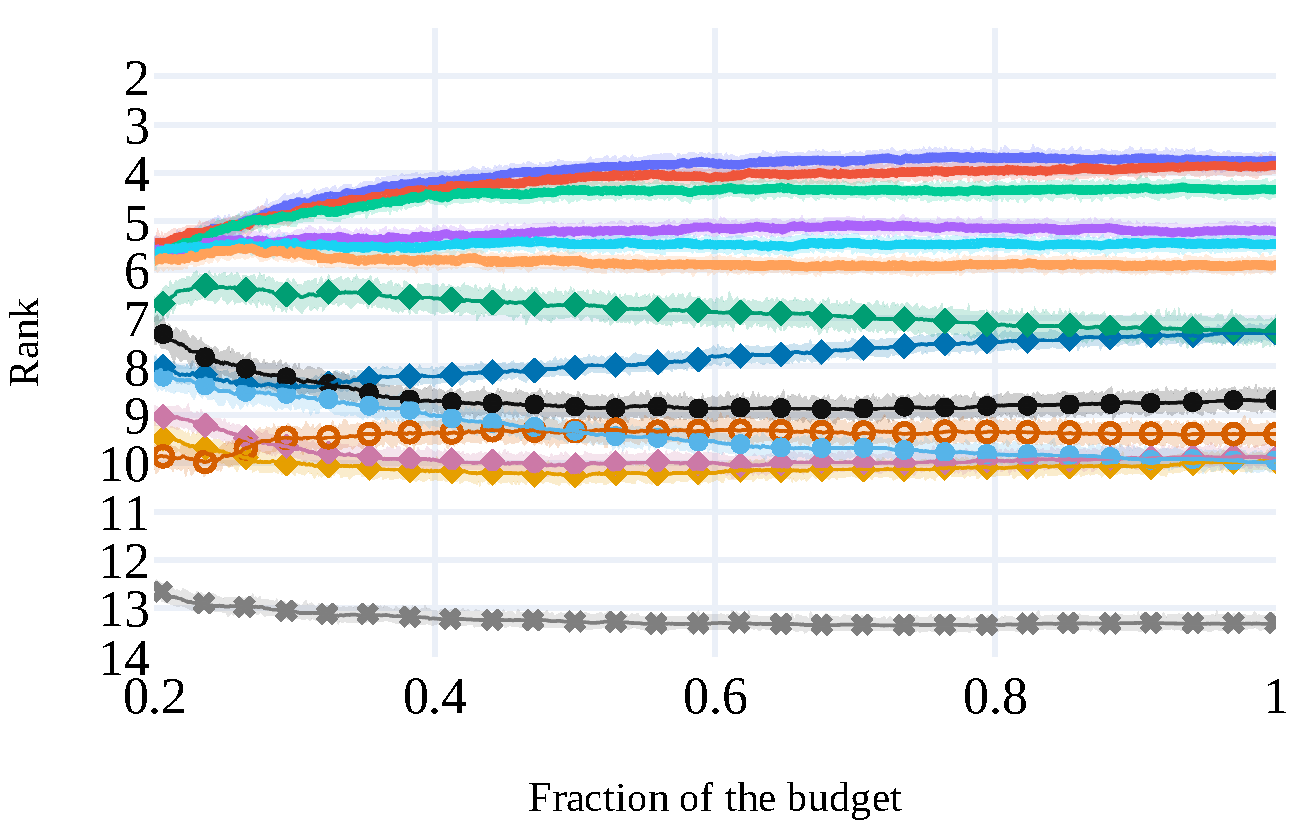
\includegraphics[scale=0.33]{figures/06/figs/figs/ranks/main_ranks_all.pdf}
%         \caption{All target functions}
%     \end{subfigure}
%     \begin{subfigure}[t]{0.49\textwidth}
%         \centering
%         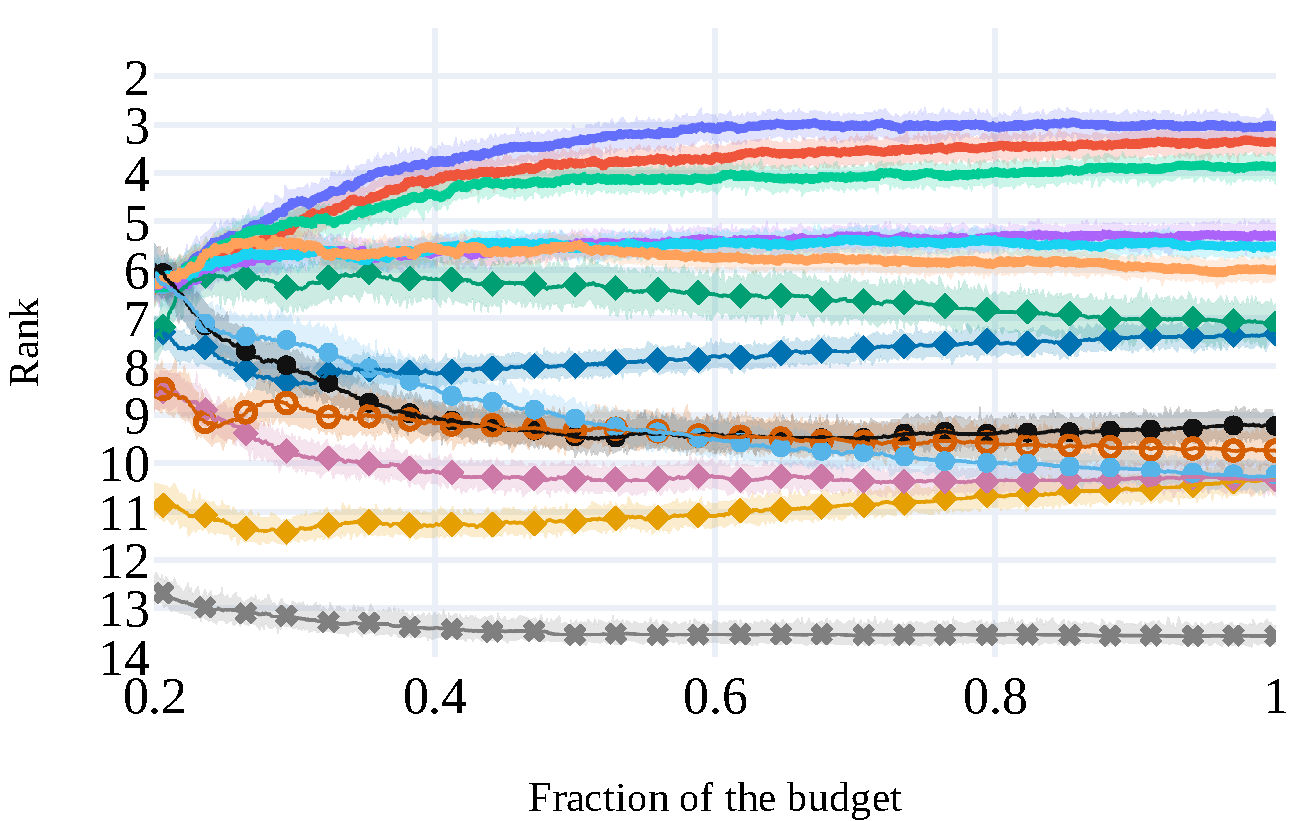
\includegraphics[scale=0.33]{figures/06/figs/figs/ranks/main_ranks_cheap.pdf}
%         \caption{Cheap (up to 10 minutes)}
%     \end{subfigure}
%     \begin{subfigure}[t]{0.49\textwidth}
%         \centering
%         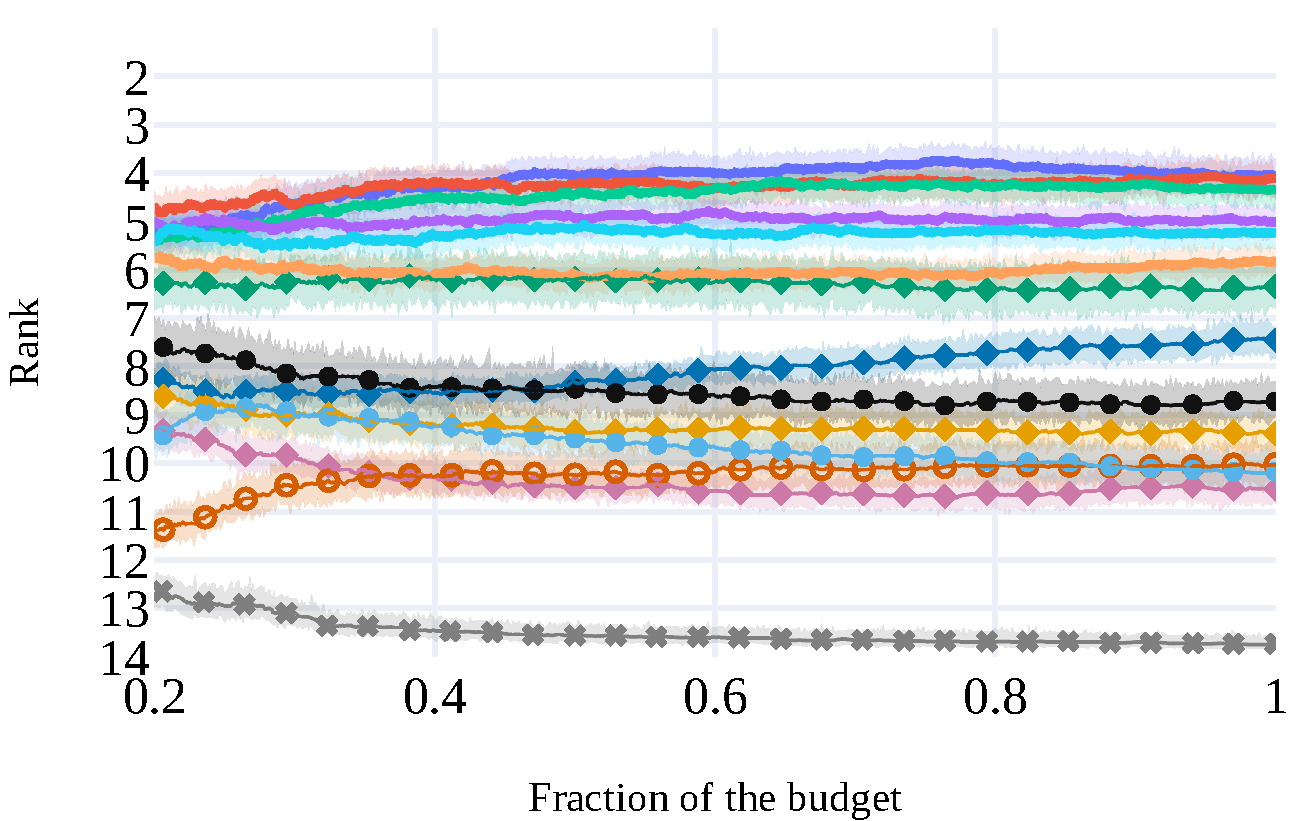
\includegraphics[scale=0.33]{figures/06/figs/figs/ranks/main_ranks_medium.pdf}
%         \caption{Medium-cost (more than 10 minutes, up to \mbox{1 hour})}
%     \end{subfigure}
%     \begin{subfigure}[t]{0.49\textwidth}
%         \centering
%         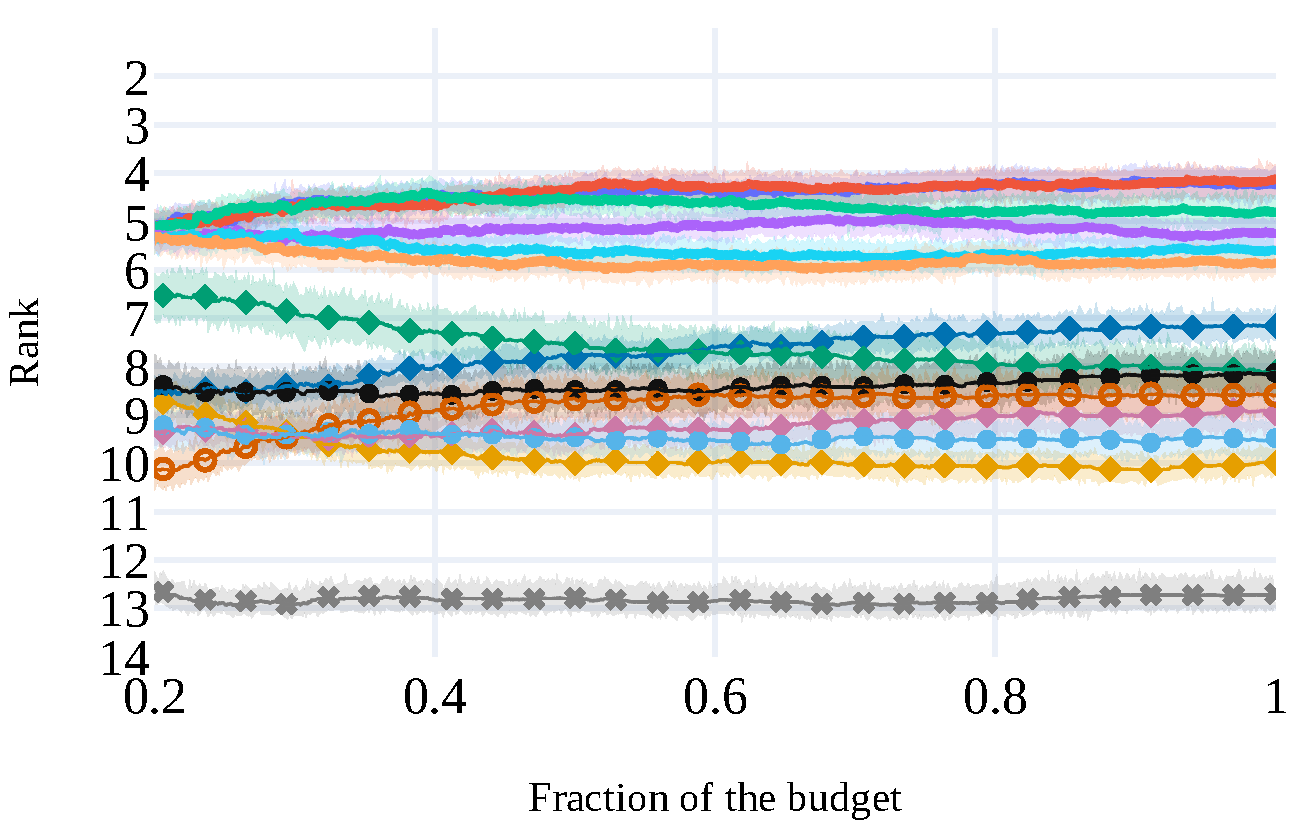
\includegraphics[scale=0.33]{figures/06/figs/figs/ranks/main_ranks_expensive.pdf}
%         \caption{Expensive (more than 1 hour)}
%     \end{subfigure}
%     \begin{subfigure}[t]{\textwidth}
%         \centering
%         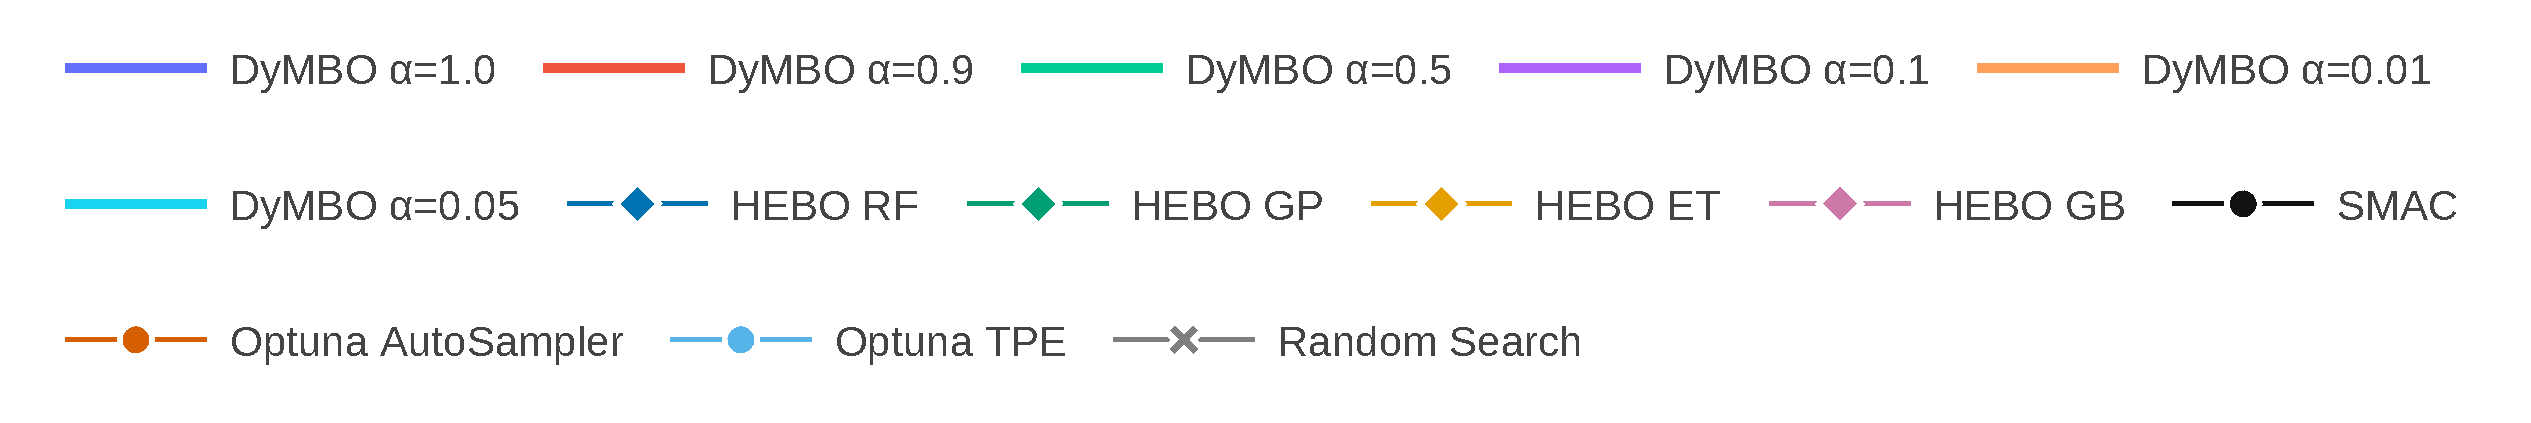
\includegraphics[scale=0.33]{figures/06/figs/figs/ranks/main_ranks_expensive_legend.pdf}
%     \end{subfigure}
%     \caption{
%     Mean ranks of \texttt{DyMBO} \changed{(with different values of $\alpha$)}, HEBO with different surrogate models, and other HPO methods on YAHPO Gym and JAHS-Bench-201, split according to different budgets: (a) all target functions, (b) cheap target functions with a budget of up to 10 minutes, (c) medium-cost target functions with a budget between 10 minutes and up to 1 hour, (d) expensive target functions with a budget of more than 1 hour. %\hh{slightly modified:}
%     % \changed{
%     Although different methods ranked differently with different target functions costs, \texttt{DyMBO} achieves the top rank across all target functions.%}
%     % \todo{Could the authors include some runs with alpha = \{0.01,0.05\}, especially for long budgets?}
%     % \hs{running}
%     % \todo{improvements: pull out the legends outside the plot and increase font size; aspect ratio to maximise usage of space with larger label fonts; colours not enough -- use markers, styles and opacity (worse algos = lower opacity); 4a) x-axis unclear -- make x-axis actual wall-clock time; choose a stronger subset of algos (especially with another BO baseline from the literature) and show primary results here, and show comprehensive results later}
%     }
%     \label{fig:gen_res}
% \end{figure*}



% \changed{
We begin by comparing \texttt{DyMBO} variants with different $\alpha$ values in~\cref{fig:ch05:gen_res_alpha}. We present the average rank as a function of the fraction of the budget for YAHPO Gym and JAHS-Bench-201. The results are split into four parts, according to the mean time required for evaluating the target function. Therefore, we show mean ranks on all target functions, on cheap functions with a budget of up to 10 minutes, on medium-cost functions with a budget
between 10 minutes up to 1 hour, and on expensive functions with a budget exceeding 1~hour. 
We observe that for cheap benchmarks, the selection variant ($\alpha=1.0$) works best, while the advantage of it compared to lower $\alpha$ values diminishes when the budget grows, whereas for expensive benchmarks, selection has similar performance to $\alpha=0.9$. Over all target functions, $\alpha=1.0$ works best.
% }


\begin{figure*}[h]
    \centering
    \begin{subfigure}[t]{0.49\textwidth}
        \centering
        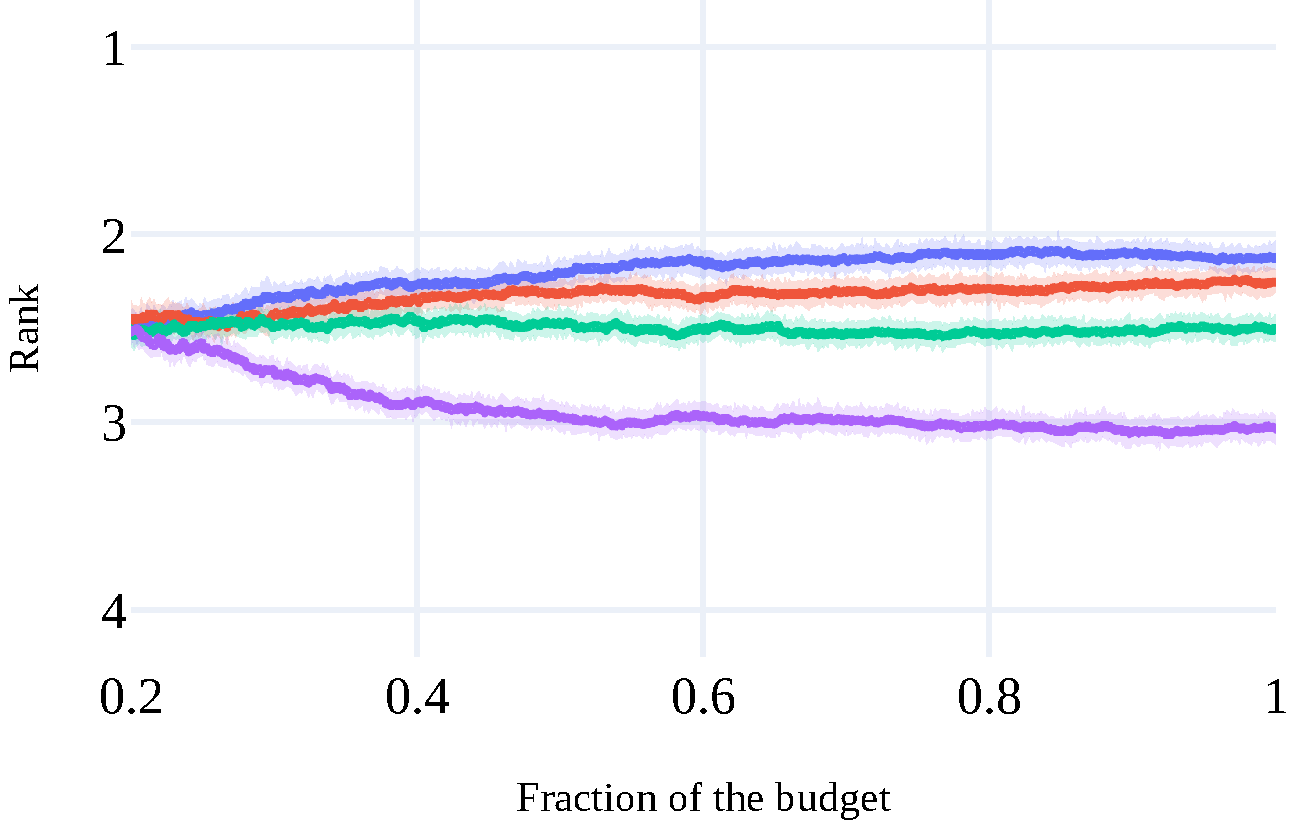
\includegraphics[scale=0.33]{figures/05/figs/figs/ranks/alpha_ablation_all.pdf}
        \caption{All target functions}
    \end{subfigure}
    \begin{subfigure}[t]{0.49\textwidth}
        \centering
        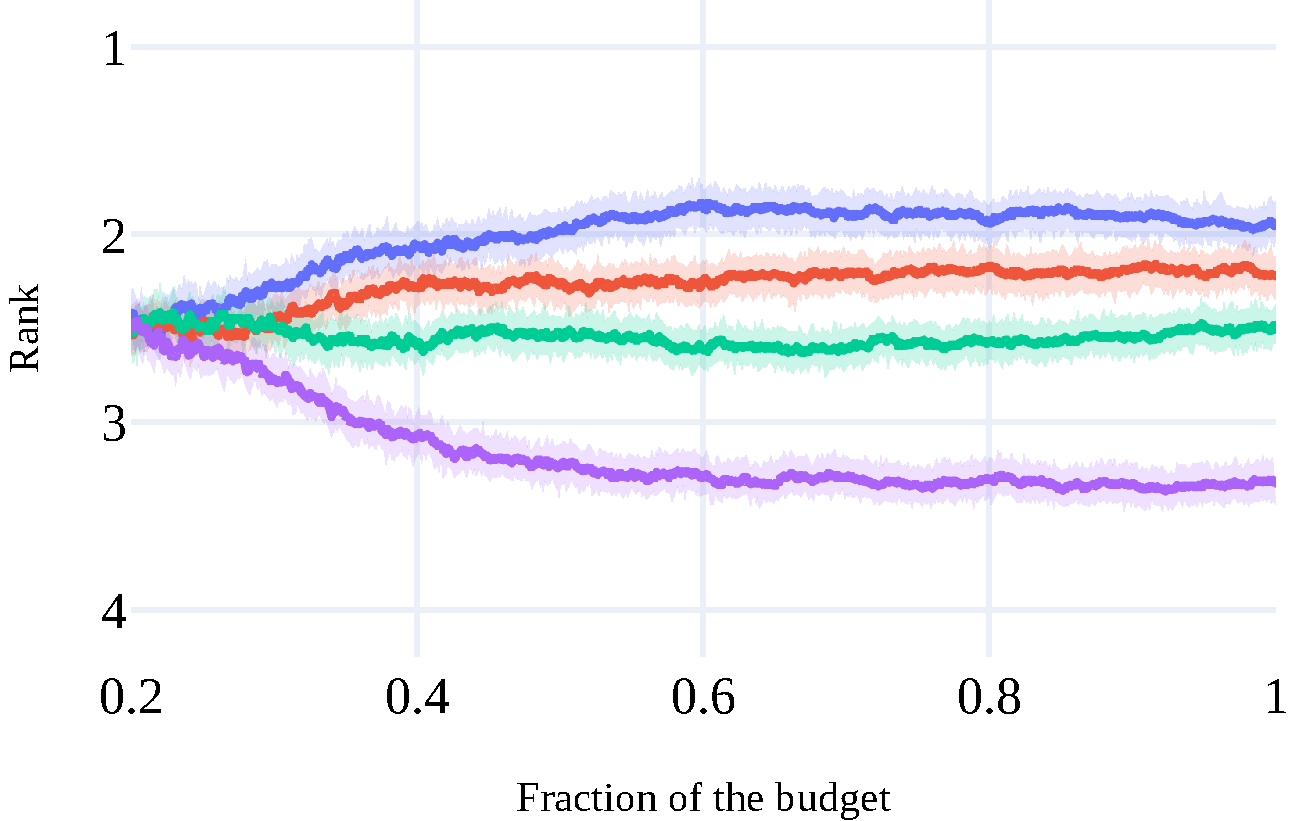
\includegraphics[scale=0.33]{figures/05/figs/figs/ranks/alpha_ablation_cheap.pdf}
        \caption{Cheap (up to 10 minutes)}
    \end{subfigure}
    \begin{subfigure}[t]{0.49\textwidth}
        \centering
        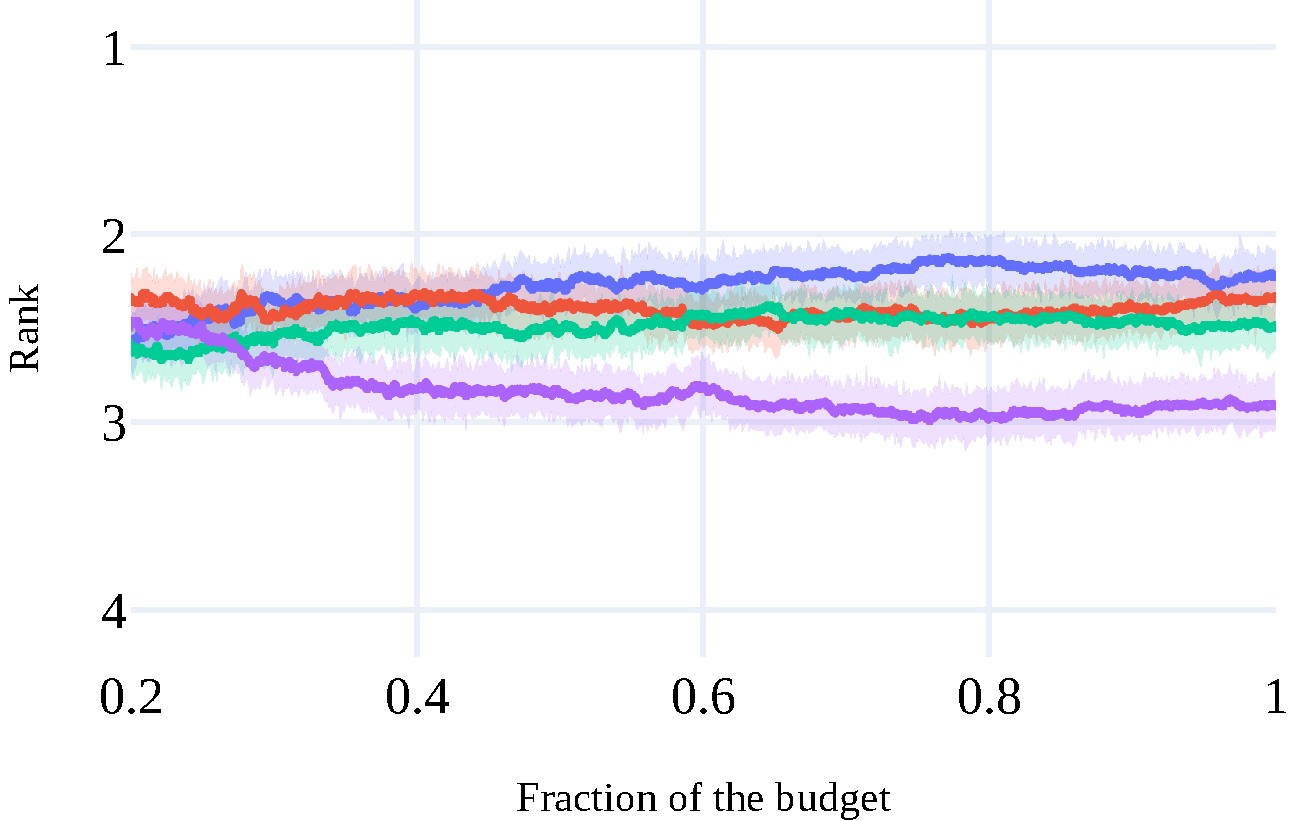
\includegraphics[scale=0.33]{figures/05/figs/figs/ranks/alpha_ablation_medium.pdf}
        \caption{Medium-cost (more than 10 minutes, up to \mbox{1 hour})}
    \end{subfigure}
    \begin{subfigure}[t]{0.49\textwidth}
        \centering
        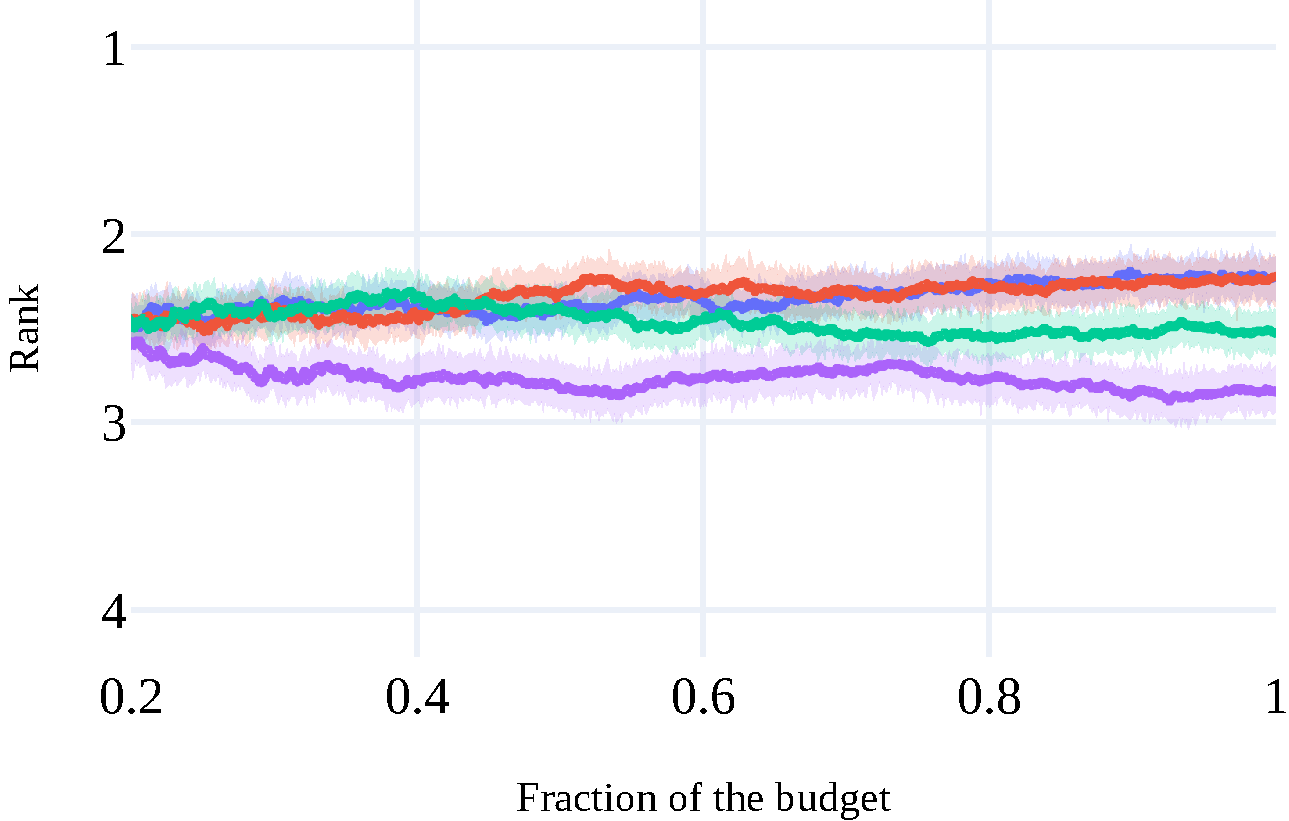
\includegraphics[scale=0.33]{figures/05/figs/figs/ranks/alpha_ablation_expensive.pdf}
        \caption{Expensive (more than 1 hour)}
    \end{subfigure}
    \begin{subfigure}[t]{\textwidth}
        \centering
        
\includegraphics[scale=0.33]{figures/05/figs/figs/ranks/alpha_ablation_all_legend.pdf}
    \end{subfigure}
    \caption{
    % \hs{
    Mean rank of \texttt{DyMBO} with ($\alpha \in {1.0, 0.9, 0.5, 0.1}$) on YAHPO Gym and JAHS-Bench-201 as a function of the fraction of the wall-clock time budget of each task. Results are shown for (a) all target functions, (b) cheap functions with budgets of up to 10 minutes, (c) medium-cost functions with budgets between 10 minutes and 1 hour, and (d) expensive functions with budgets exceeding 1 hour. Lower ranks indicate better performance. The greedy selection variant ($\alpha=1.0$) achieves the best overall mean rank, while its advantage decreases for more expensive target functions.
    % }
    }
    \label{fig:ch05:gen_res_alpha}
\end{figure*}

% \hs{
% We begin by comparing the different \texttt{DyMBO} variants with different $\alpha$ values in~\autoref{fig:gen_res_alpha}. We present the average rank as a function of the fraction of the budget for YAHPO Gym and JAHS-Bench-201. The results are split into four parts according to the mean time required for evaluating the target function. Therefore, we show mean ranks on all target functions, on cheap functions with a budget of up to 10 minutes, on medium-cost functions with a budget
% between 10 minutes up to 1 hour, and on expensive functions with a budget exceeding 1 hour. 
% We observed that for cheap benchmarks, $\alpha=1.0$, the selection variant works best, while the advantage of it compared to other $\alpha$ values diminishes when the budget grows, as for expensive benchmarks, it has similar performance to $\alpha=0.9$. Over all target functions, $\alpha=1.0$ works best.
% }
\begin{figure*}[h]
    \centering
    \begin{subfigure}[t]{0.49\textwidth}
        \centering
        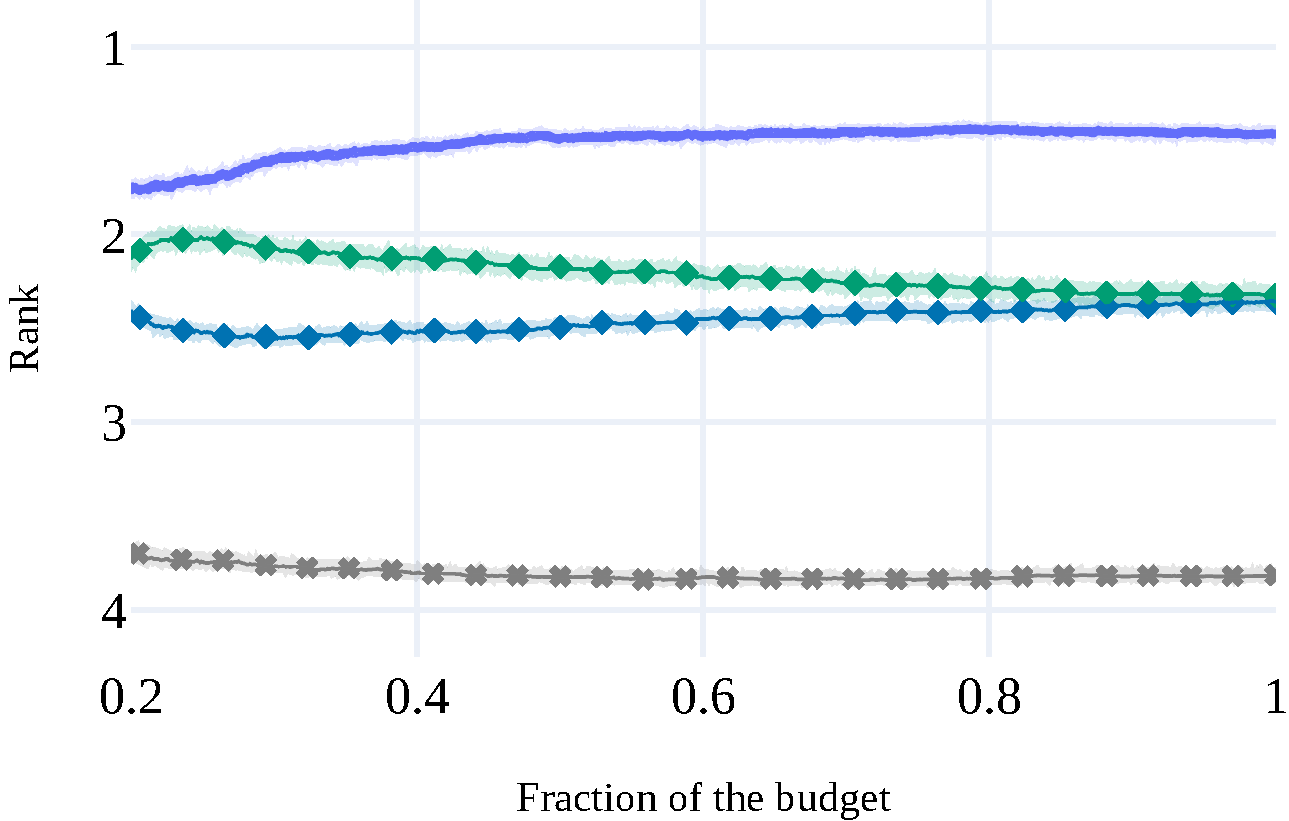
\includegraphics[scale=0.33]{figures/05/figs/figs/ranks/main_ranks_simple2_all.pdf}
        \caption{All target functions}
    \end{subfigure}
    \begin{subfigure}[t]{0.49\textwidth}
        \centering
        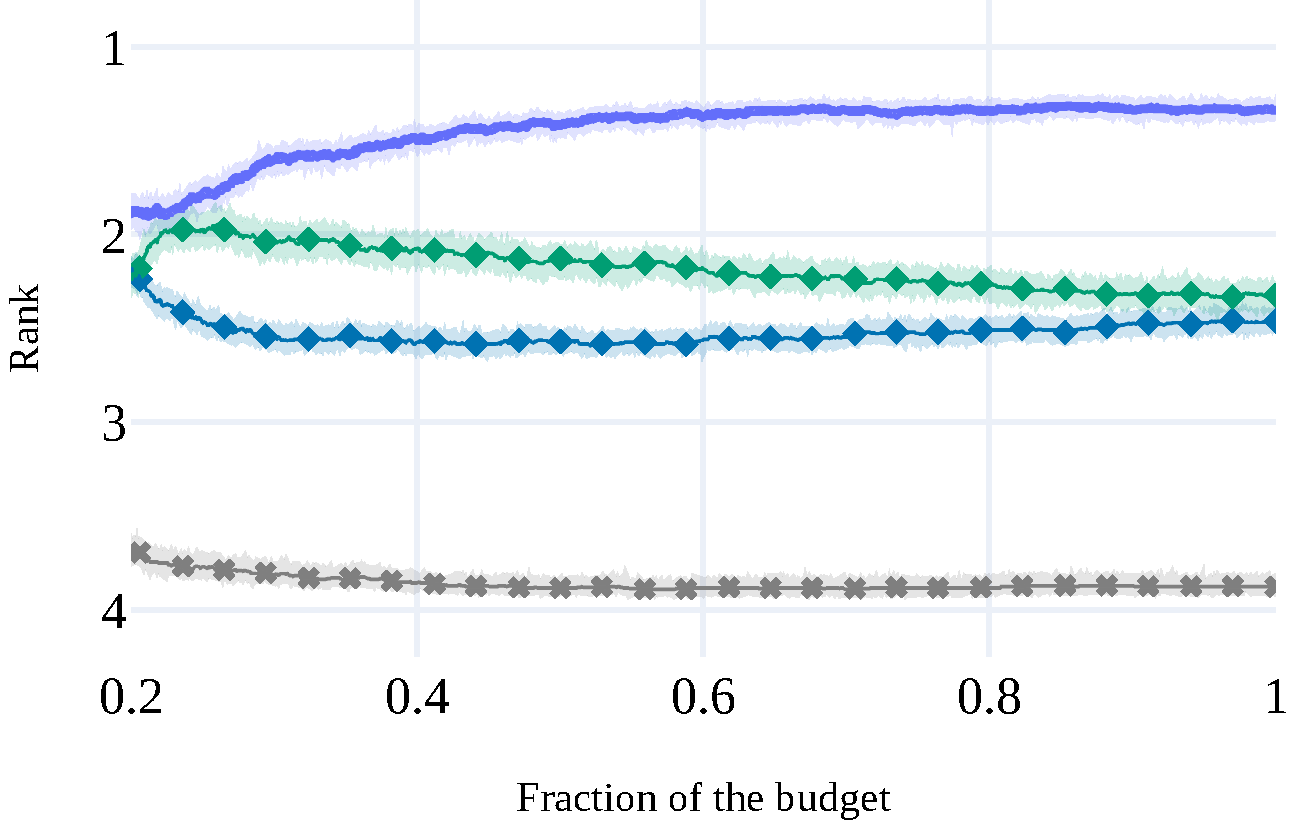
\includegraphics[scale=0.33]{figures/05/figs/figs/ranks/main_ranks_simple2_cheap.pdf}
        \caption{Cheap (up to 10 minutes)}
    \end{subfigure}
    \begin{subfigure}[t]{0.49\textwidth}
        \centering
        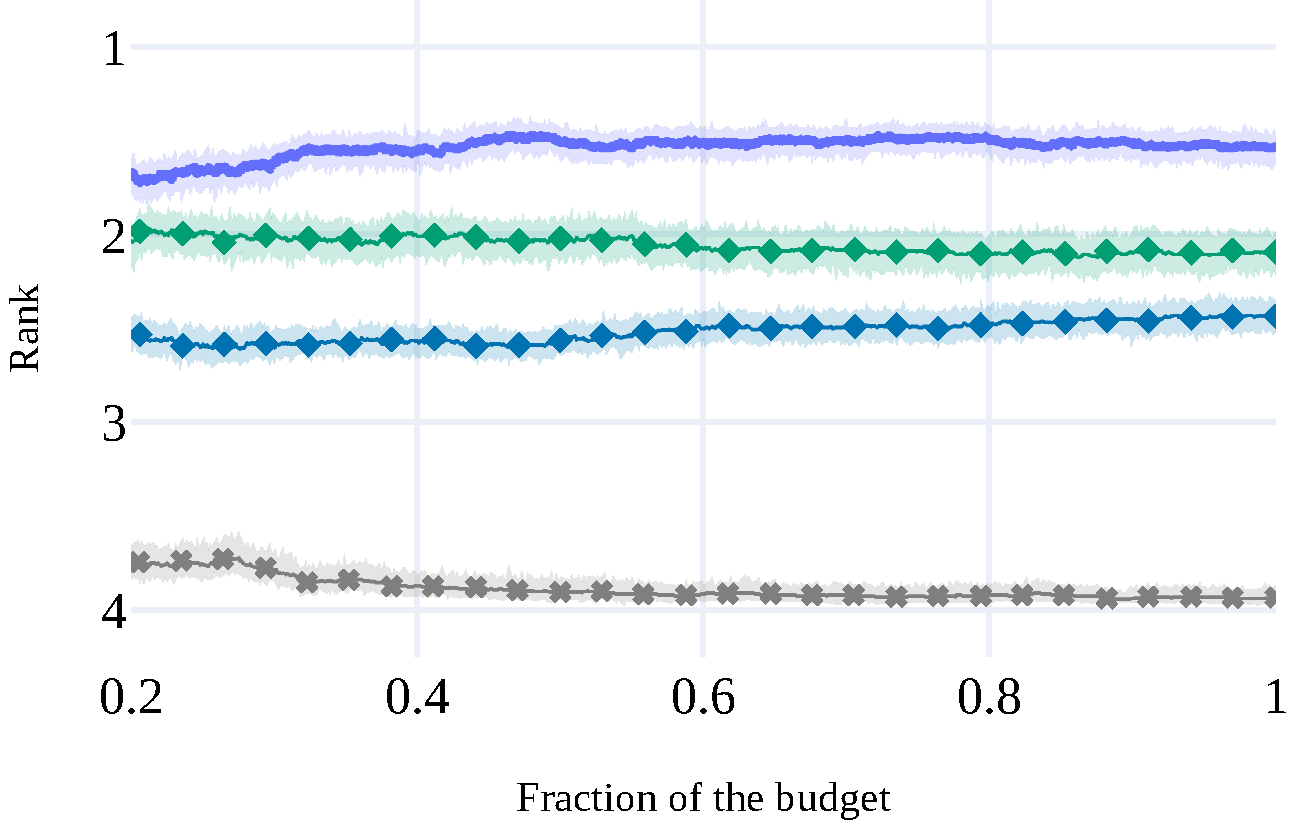
\includegraphics[scale=0.33]{figures/05/figs/figs/ranks/main_ranks_simple2_medium.pdf}
        \caption{Medium-cost (more than 10 minutes, up to \mbox{1 hour})}
    \end{subfigure}
    \begin{subfigure}[t]{0.49\textwidth}
        \centering
        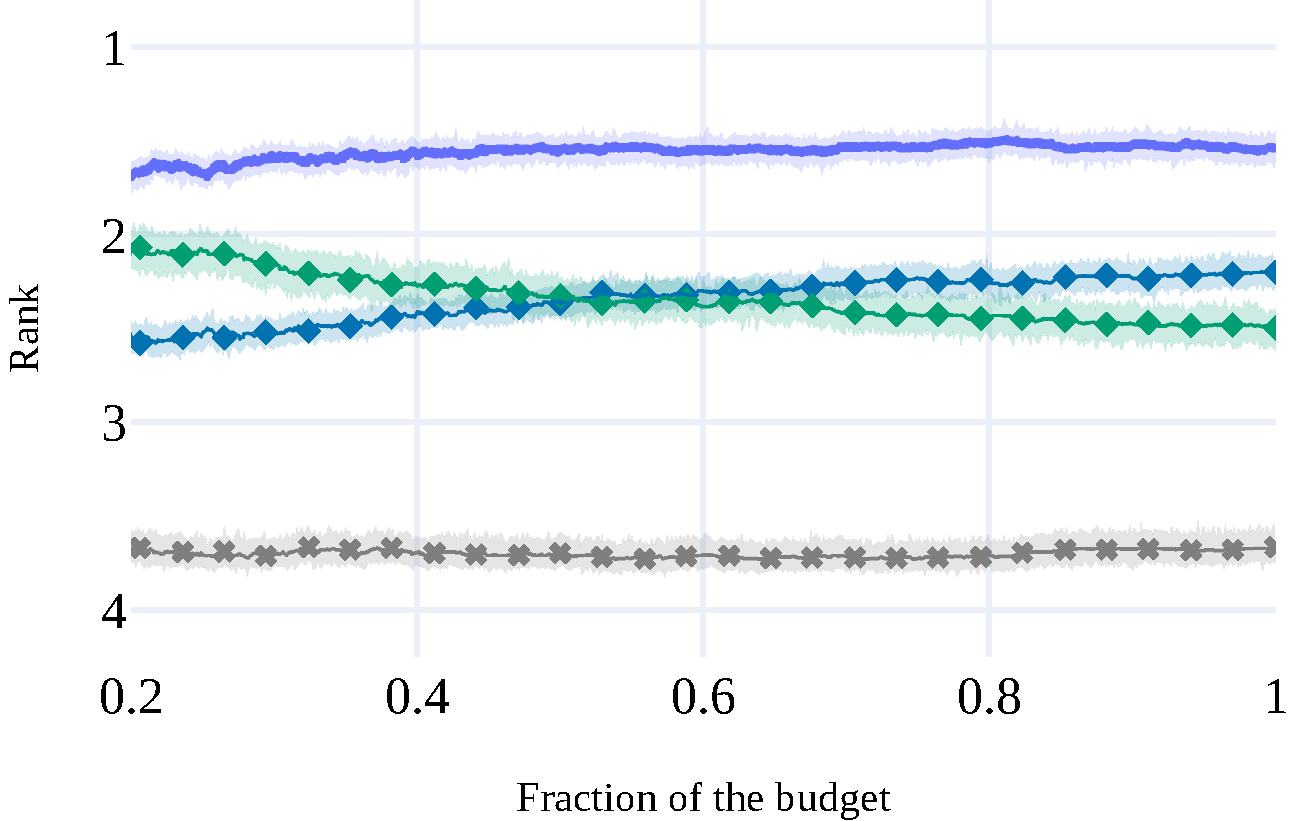
\includegraphics[scale=0.33]{figures/05/figs/figs/ranks/main_ranks_simple2_expensive.pdf}
        \caption{Expensive (more than 1 hour)}
    \end{subfigure}
    \begin{subfigure}[t]{\textwidth}
        \centering
        
\includegraphics[scale=0.33]{figures/05/figs/figs/ranks/main_ranks_simple2_all_legend.pdf}
    \end{subfigure}
    \caption{
    % \hs{
    Mean rank of \texttt{DyMBO} with ($\alpha=1.0$), HEBO with RF and GP surrogates, and random search on YAHPO Gym and JAHS-Bench-201 as a function of the fraction of the wall-clock time budget of each task. Results are shown for (a) all target functions, (b) cheap functions with budgets of up to 10 minutes, (c) medium-cost functions with budgets between 10 minutes and 1 hour, and (d) expensive functions with budgets exceeding 1 hour. Lower ranks indicate better performance. \texttt{DyMBO} achieves the best mean rank in all budget groups, while the relative performance of the RF and GP baselines varies across groups.
    % }
    }
    \label{fig:ch05:gen_res_simple}
\end{figure*}

\begin{figure*}[h]
    \centering
    \begin{subfigure}[t]{0.49\textwidth}
        \centering
        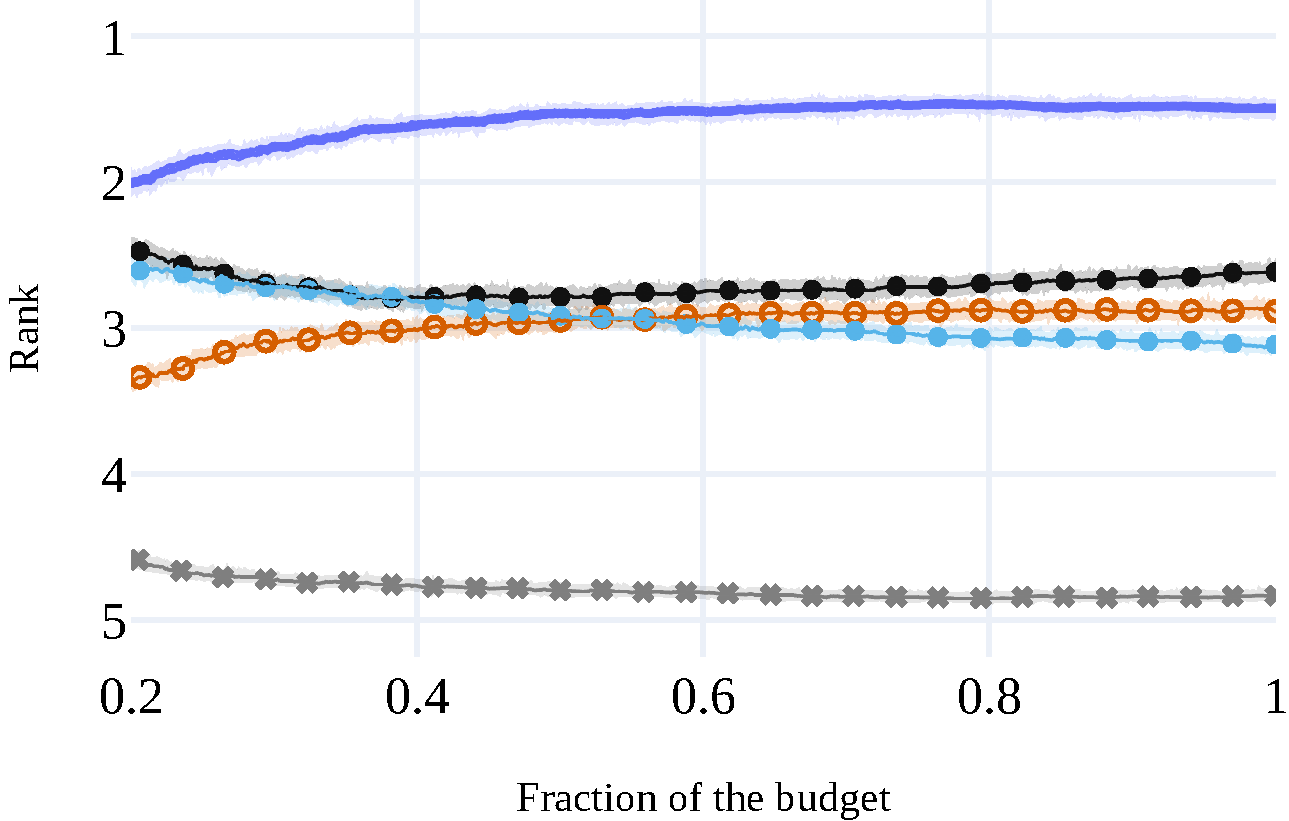
\includegraphics[scale=0.33]{figures/05/figs/figs/ranks/main_ranks_other_baselines2_all.pdf}
        \caption{All target functions}
    \end{subfigure}
    \begin{subfigure}[t]{0.49\textwidth}
        \centering
        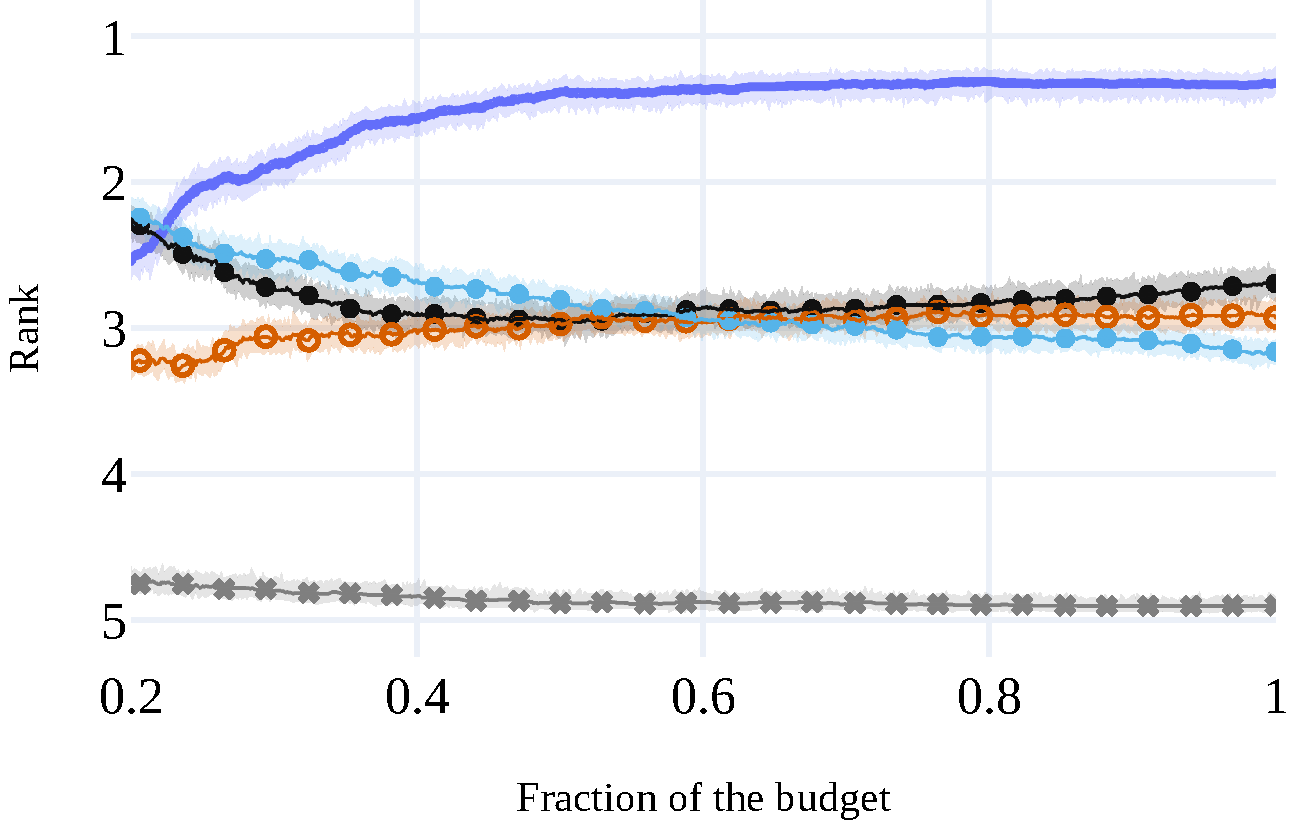
\includegraphics[scale=0.33]{figures/05/figs/figs/ranks/main_ranks_other_baselines2_cheap.pdf}
        \caption{Cheap (up to 10 minutes)}
    \end{subfigure}
    \begin{subfigure}[t]{0.49\textwidth}
        \centering
        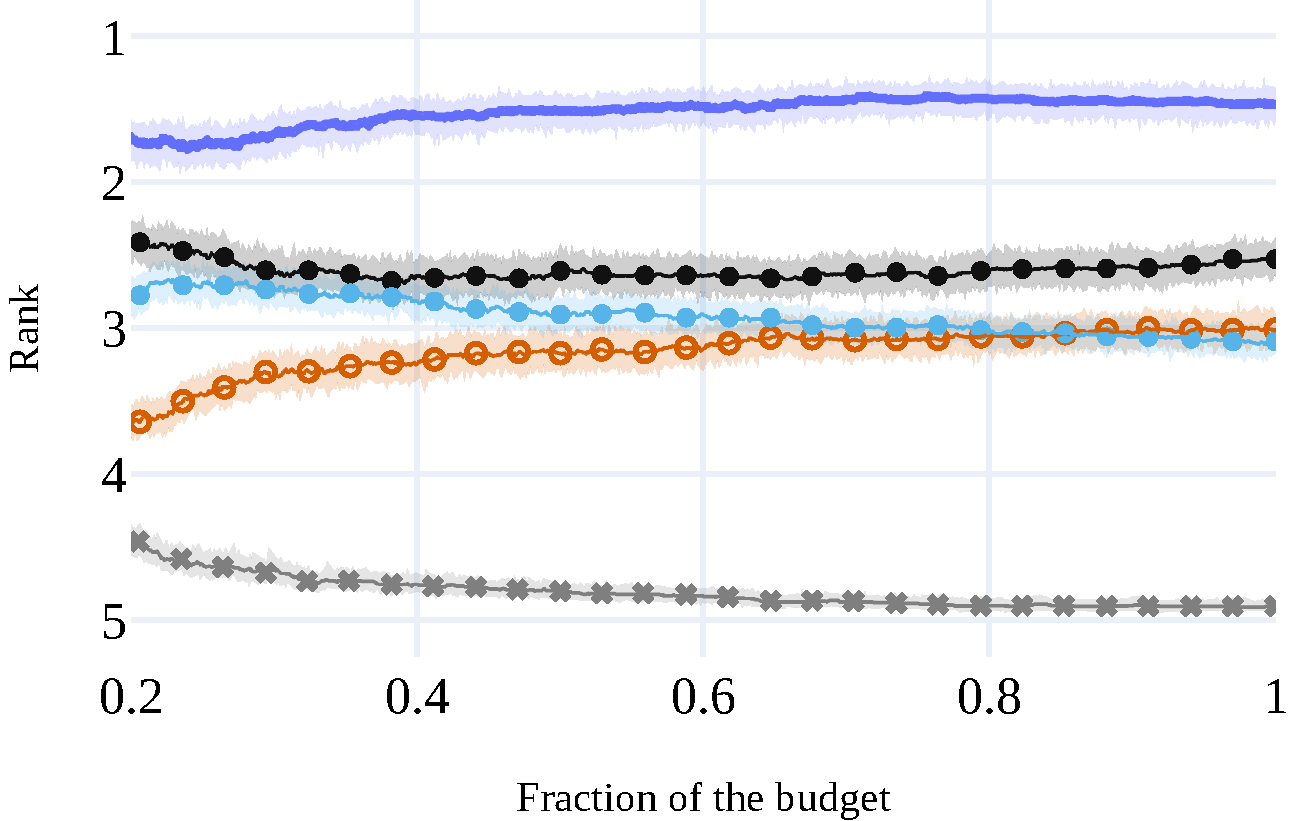
\includegraphics[scale=0.33]{figures/05/figs/figs/ranks/main_ranks_other_baselines2_medium.pdf}
        \caption{Medium-cost (more than 10 minutes, up to \mbox{1 hour})}
    \end{subfigure}
    \begin{subfigure}[t]{0.49\textwidth}
        \centering
        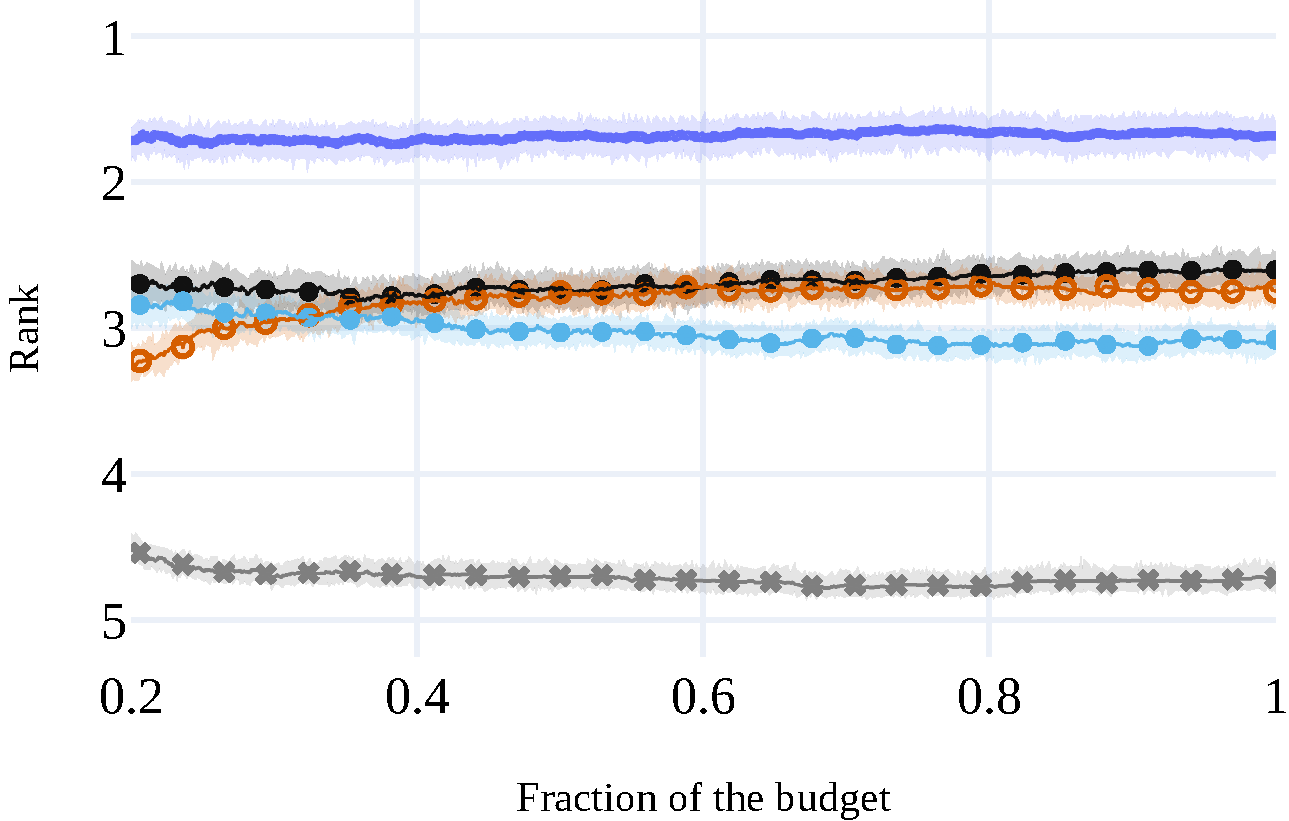
\includegraphics[scale=0.33]{figures/05/figs/figs/ranks/main_ranks_other_baselines2_expensive.pdf}
        \caption{Expensive (more than 1 hour)}
    \end{subfigure}
    \begin{subfigure}[t]{\textwidth}
        \centering
        
\includegraphics[scale=0.33]{figures/05/figs/figs/ranks/main_ranks_other_baselines2_all_legend.pdf}
    \end{subfigure}
    \caption{
    Mean rank of \texttt{DyMBO} with ($\alpha=1.0$), SMAC, Optuna AutoSampler, Optuna TPE, and random search on YAHPO Gym and JAHS-Bench-201 as a function of the fraction of the wall-clock time budget of each task. Results are shown for (a) all target functions, (b) cheap functions with budgets of up to 10 minutes, (c) medium-cost functions with budgets between 10 minutes and 1 hour, and (d) expensive functions with budgets exceeding 1 hour. Lower ranks indicate better performance. \texttt{DyMBO} achieves the best mean rank throughout the optimisation across all budget groups.
    }
    \label{fig:ch05:gen_res_baselines}
\end{figure*}

% \hs{
We continue our evaluation by comparing the best \texttt{DyMBO} variant with HEBO with single surrogates, which is shown in~\cref{fig:ch05:gen_res_simple}.
The results demonstrate that \texttt{DyMBO} achieves a better mean rank compared the HEBO with RF and GP across all budget categories. While for cheap and medium-cost functions GP works well, for the expensive functions, RF works well when more than $50\%$ of the budget has been spent, showing the performance complementarity between the different surrogates. As expected, random search consistently performs worst. Comparing \texttt{DyMBO} to additional baselines, namely TPE as implemented in Optuna, AutoSampler of Optuna and SMAC, we observe in~\cref{fig:ch05:gen_res_baselines} that \texttt{DyMBO} outperforms all of these baselines on average, as SMAC emerges as the second best method, followed by Optuna AutoSampler and Optuna TPE.
% }
% \aj{unresolved ref for fig}

% \er{Can you remind me the reason why we choose the total budget based on time and not evaluations?}\hs{it's HPO, that's a common practice: if we use more time for the optimiser we have less time for the target function}
% We also present an analysis of the statistical significance of our results. 


\begin{figure}[h]
    \centering
    \begin{subfigure}[t]{0.49\textwidth}
        \centering
        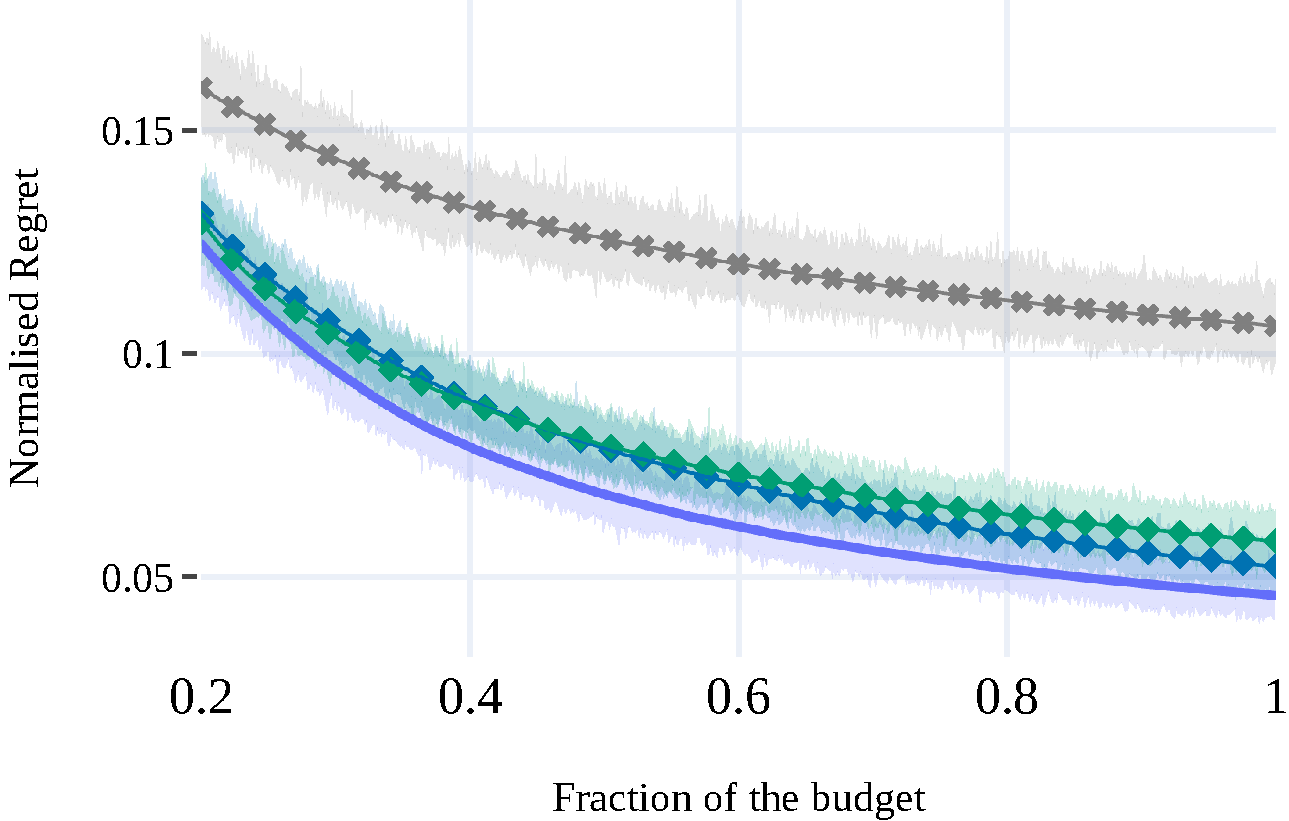
\includegraphics[scale=0.33]{figures/05/figs/figs/ranks/main_ranks_simple2_all_val.pdf}
        \caption{}
    \end{subfigure}
    \begin{subfigure}[t]{0.49\textwidth}
        \centering
        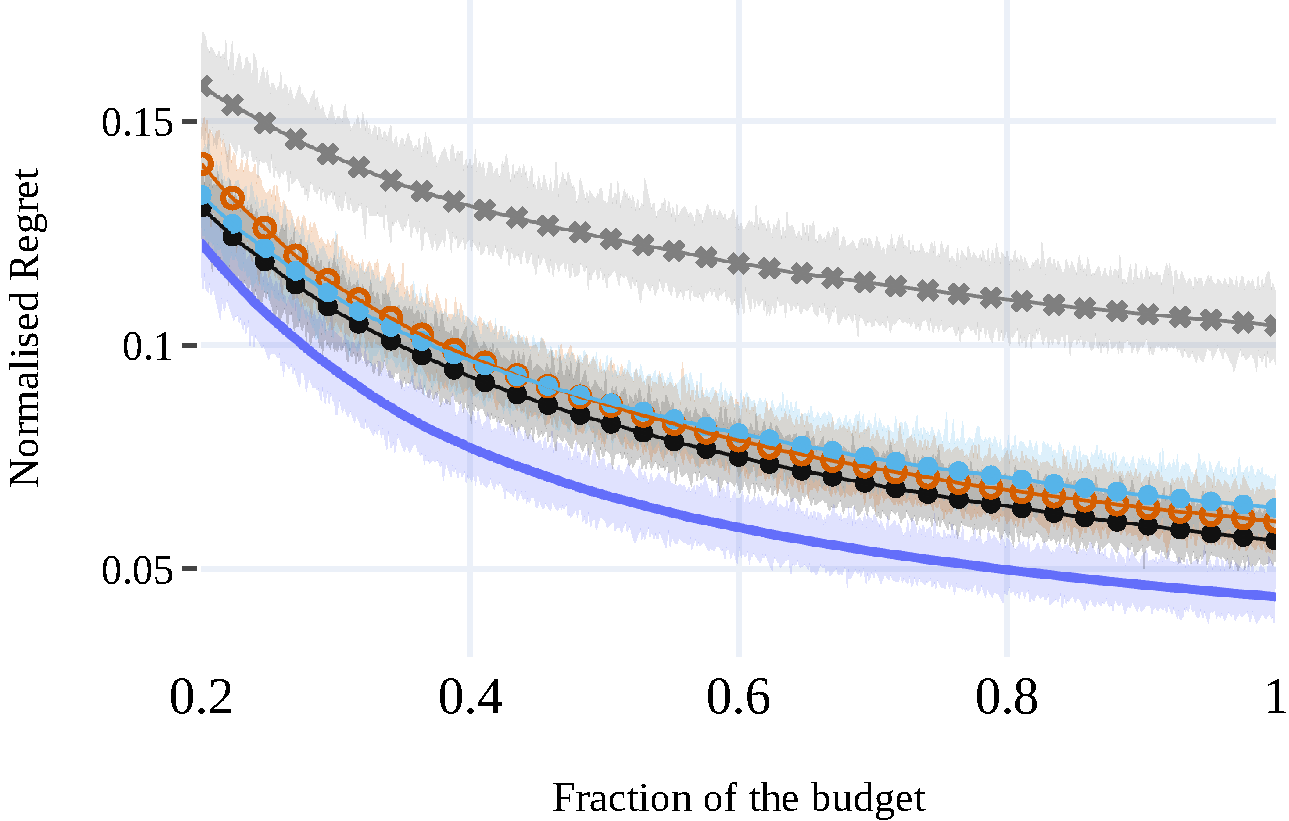
\includegraphics[scale=0.33]{figures/05/figs/figs/ranks/main_ranks_other_baselines2_all_val.pdf}
        \caption{}
    \end{subfigure}
    \begin{subfigure}[t]{0.49\textwidth}
        \centering
        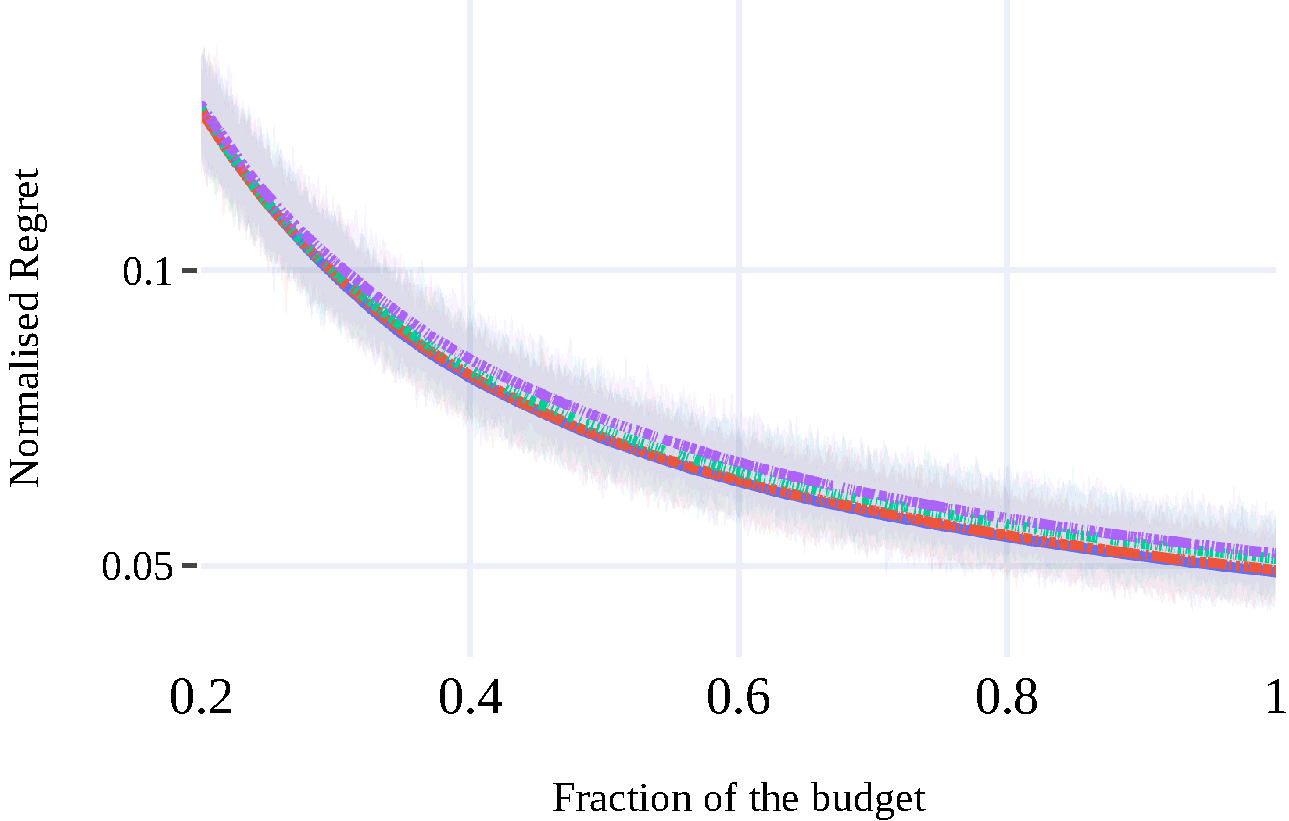
\includegraphics[scale=0.33]{figures/05/figs/figs/ranks/alpha_ablation_all_val.pdf}
        \caption{}
    \end{subfigure}
    \begin{subfigure}[t]{0.49\textwidth}
        \centering
        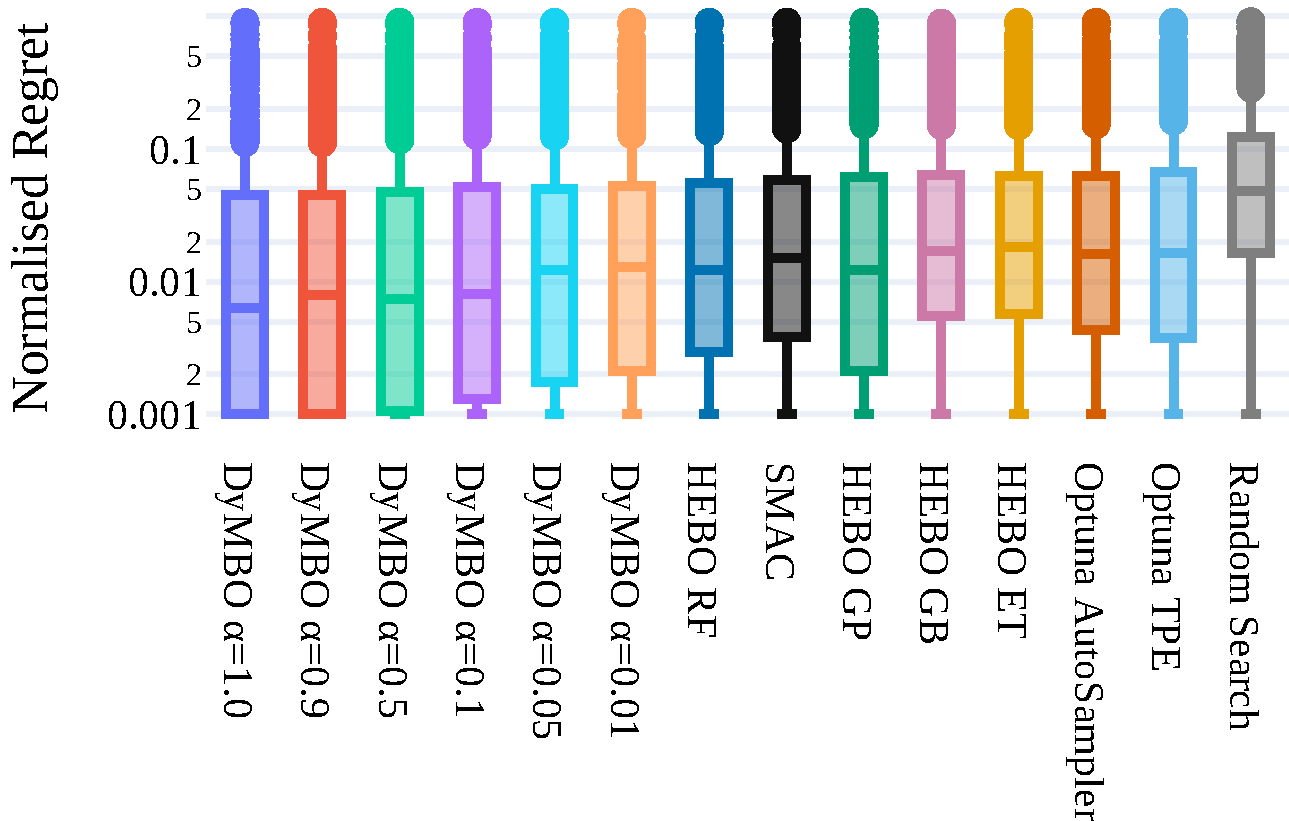
\includegraphics[scale=0.33]{figures/05/figs/figs/ranks/box_plot.pdf}
        \caption{}
    \end{subfigure}
    \begin{subfigure}[t]{\textwidth}
        \centering
        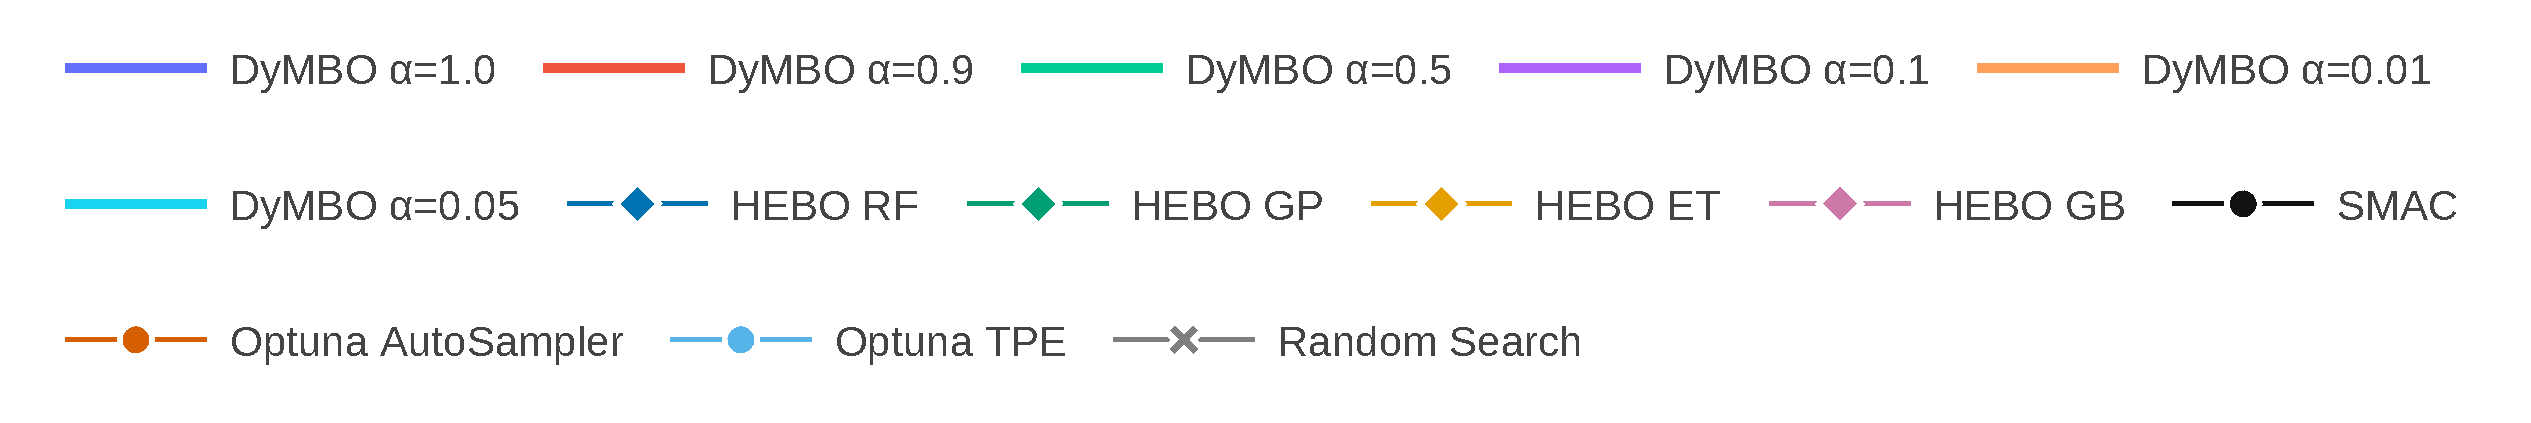
\includegraphics[scale=0.33]{figures/05/figs/figs/ranks/main_ranks_all_val_legend.pdf}
        % \caption{}
    \end{subfigure}
    % 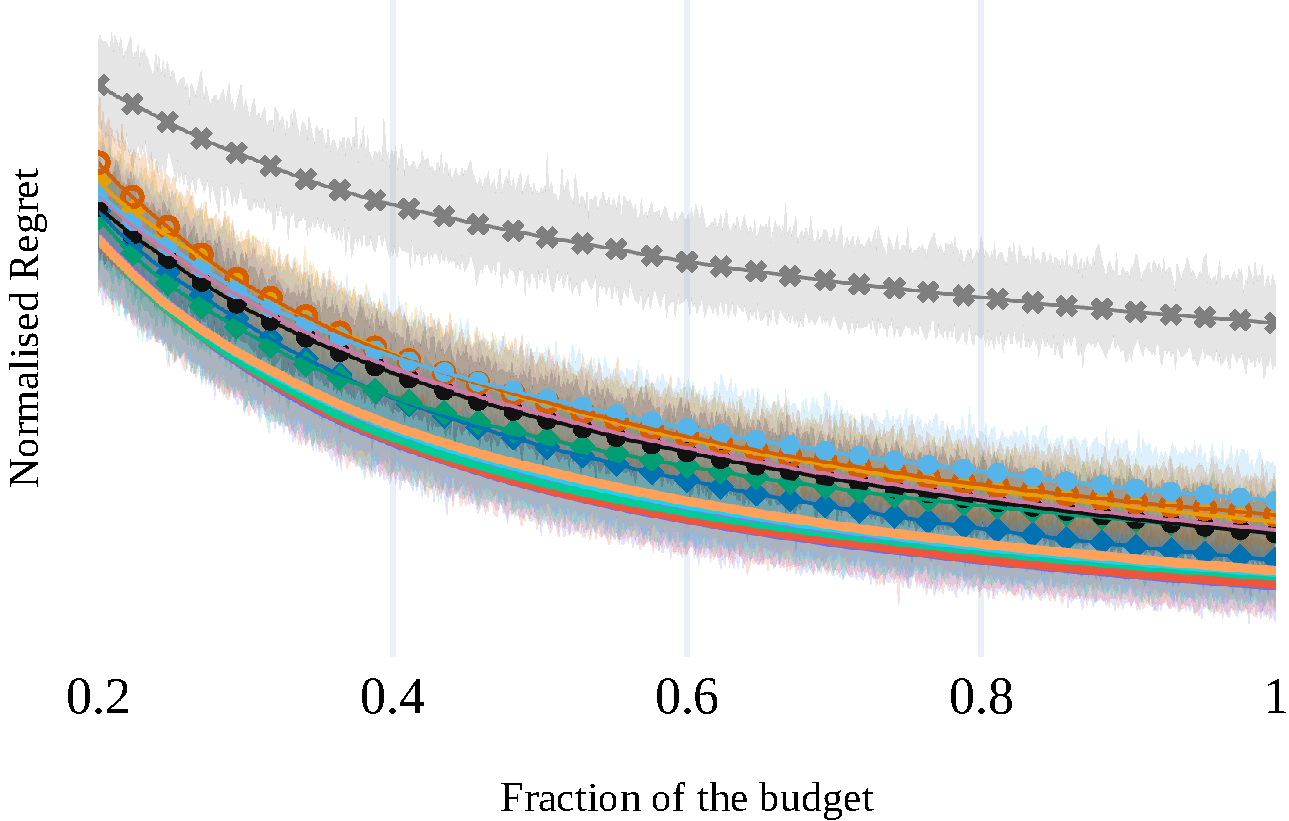
\includegraphics[scale=0.33]{figures/06/figs/figs/ranks/main_ranks_all_val.pdf}
    \caption{%\changed{
    Normalised regret on YAHPO Gym and JAHS-Bench-201 as a function of the fraction of the wall-clock time budget of each task. Panels compare (a) \texttt{DyMBO} with $\alpha=1.0$ against single-surrogate HEBO variants and random search, (b) \texttt{DyMBO} with $\alpha=1.0$ against other HPO frameworks and random search, and (c) \texttt{DyMBO} variants with different values of $\alpha$. Panel (d) shows the distribution of final normalised regret for all methods on a logarithmic scale. Lower normalised regret indicates better performance. \texttt{DyMBO} with $\alpha=1.0$ attains the lowest mean regret and a favourable distribution of final regret relative to the baselines.
    }
    % }
    \label{fig:ch05:mean_reg}
\end{figure}

% \changed{
We present the mean normalised regret of all methods in~\cref{fig:ch05:mean_reg}. Normalised regret is calculated per function, using min-max normalisation with the minimum and maximum value found by all optimisers. 
We performed such normalisation as the values of different functions are in different ranges and scales. We observe lower mean regret for \texttt{DyMBO} compared to the other methods, confirming the results reported by the mean ranks.
% }

% \hh{Minor changes in wording -- check carefully:}
% \changed{
When considering all target functions, we see that \texttt{DyMBO} achieves a better mean rank than the baselines, both those using HEBO and those using other HPO frameworks. When partitioning our set of target functions according to the evaluation budget, we observe different ranks for the single-surrogate HEBO variants. For example, for cheap functions, RF performs better on average than GP on full budget, while GP performs better than RF for the medium budget functions. Despite that, \texttt{DyMBO} is ranked above both HEBO with RFs and HEBO with GPs for all budget categories.

% \changed{The following was in the appendix:}
We tested the statistical significance of our results 
% presented in \autoref{sec:res_general},
% \changed{
and we observe that \texttt{DyMBO} (across both the ensembling and selection variants) 
% }
significantly outperforms single-surrogate-based BO and other considered HPO methods. 
To do this, we used the best-found target function values per optimiser. 
We then calculated the mean value for each pair of function and optimiser over the 51 random seeds. 
The optimiser that has the best value per function is then considered as the best for the particular function. 
We calculated whether the values obtained for each of the other optimisers are statistically equal to the values of the best optimiser using a permutation test with 10\,000 samples and a significance level of $0.05$. 
We report these results in~\cref{tab:ch05:stat_signif}. 
We see that \texttt{DyMBO} achieves equal performance to the best method more times than any other baseline, across all budget groups. 
\texttt{DyMBO} with $\alpha = 1.0$ is statistically tied with the best method in 724 cases, followed by a monotonically decreasing number of ties as $\alpha$ decreases, but remaining statistically significantly better than non-\texttt{DyMBO} methods.
% second-best
The best non-\texttt{DyMBO} method is HEBO using GP with 363 cases. We performed the Wilcoxon sign test on the results of the permutations test, such that for every benchmark we assign 1 when the method is statistically tied with the best method, otherwise we assign 0. We found that 
% \changed{
all variants of \texttt{DyMBO} with different $\alpha$ values are significantly better than all other baselines.
We therefore conclude that \texttt{DyMBO} significantly outperforms any other baseline.
% }

\begin{table}[h]
    \centering
        \caption{
        Win/tie counts of different BO-based approaches, including \texttt{DyMBO}, single-surrogate HEBO baselines, and other HPO methods, per function category (\emph{i.e.}, all, cheap, medium-cost, and expensive functions).
        We report the number of benchmark instances (out of the total across all seeds and functions) for which the method is statistically indistinguishable from the best-performing method under a permutation test with a significance level of $0.05$. All \texttt{DyMBO} variants are significantly better than any other baseline.
        % \aj{Table 1 conspicuously lacks a static ensemble baseline or an explicitly greedy ensemble baseline.}
        % \todo{add these baselines if available, I hope we can run them if not}\hs{we have the results (appendix E). In this figure we only compare to previously published baselines. Will add significance to it as well}
        % \todo{Critical difference usually shows the difference in mean ranks and if they are pairwise significant. Could the authors please explain more about how to read Table 1?}
        }

    \begin{tabular}{llrrrr}
\toprule
Model & All & Cheap & Medium & Expensive \\
\midrule
 DyMBO $\alpha=0.1$ & 518 & 156 & 158 & 204 \\
 DyMBO $\alpha=0.5$ & 678 & 238 & 190 & 250 \\
 DyMBO $\alpha=0.9$ & 714 & 261 & 193 & \textbf{260} \\
 DyMBO $\alpha=1.0$ & \textbf{724} & \textbf{272} & \textbf{200} & 252 \\
 ET & 142 & 32 & 57 & 53 \\
 GB & 113 & 19 & 28 & 66 \\
 GP & 363 & 103 & 133 & 127 \\
 RF & 277 & 63 & 84 & 130 \\
 Optuna AutoSampler & 181 & 45 & 38 & 98 \\
 Optune TPE & 139 & 26 & 32 & 81 \\
 Random Search & 35 & 6 & 0 & 29 \\
 SMAC & 222 & 47 & 65 & 110 \\
\bottomrule
\end{tabular}
    \label{tab:ch05:stat_signif}
\end{table}

All figures (convergence plots, weight evolution and performance comparison), including results for JAHS-Bench-201, are available in the supplemental Git repository (see~\cref{sec:code-availability})
due to reasons of space.
% as there are 859 such figures. 
We provide convergence plots in~\cref{fig:ch05:full_res,fig:ch05:full_res2} for a subset of YAHPO Gym, namely the YAHPO-SO benchmark suite that contains 20 HPO problems from different scenarios. 
Additionally, we provide results for raw benchmarks (such as HPOBench) and synthetic benchmarks in~\cref{sec:ch05:add-bench}.


% \section{Weights evolution}

\begin{figure*}
    \centering
   
\begin{subfigure}[t]{0.32\textwidth}
        \centering
        \includegraphics[scale=0.33]{figures/05/figs/figs/co/co_8_init_srbv2\_rparti40499_time.pdf}
        \caption{rbv2\_rpart 40499}
    \end{subfigure}
\begin{subfigure}[t]{0.32\textwidth}
        \centering
        \includegraphics[scale=0.33]{figures/05/figs/figs/co/co_8_init_srbv2\_superi1053_time.pdf}
        \caption{rbv2\_super 1053}
    \end{subfigure}
\begin{subfigure}[t]{0.32\textwidth}
        \centering
        \includegraphics[scale=0.33]{figures/05/figs/figs/co/co_8_init_srbv2\_superi1457_time.pdf}
        \caption{rbv2\_super 1457}
    \end{subfigure}
\begin{subfigure}[t]{0.32\textwidth}
        \centering
        \includegraphics[scale=0.33]{figures/05/figs/figs/co/co_8_init_srbv2\_superi1063_time.pdf}
        \caption{rbv2\_super 1063}
    \end{subfigure}
\begin{subfigure}[t]{0.32\textwidth}
        \centering
        \includegraphics[scale=0.33]{figures/05/figs/figs/co/co_8_init_srbv2\_superi1479_time.pdf}
        \caption{rbv2\_super 1479}
    \end{subfigure}
\begin{subfigure}[t]{0.32\textwidth}
        \centering
        \includegraphics[scale=0.33]{figures/05/figs/figs/co/co_8_init_srbv2\_superi15_time.pdf}
        \caption{rbv2\_super 15}
    \end{subfigure}
\begin{subfigure}[t]{0.32\textwidth}
        \centering
        \includegraphics[scale=0.33]{figures/05/figs/figs/co/co_8_init_srbv2\_superi1468_time.pdf}
        \caption{rbv2\_super 1468}
    \end{subfigure}
\begin{subfigure}[t]{0.32\textwidth}
        \centering
        \includegraphics[scale=0.33]{figures/05/figs/figs/co/co_8_init_srbv2\_xgboosti12_time.pdf}
        \caption{rbv2\_xgboost 12}
    \end{subfigure}
\begin{subfigure}[t]{0.32\textwidth}
        \centering
        \includegraphics[scale=0.33]{figures/05/figs/figs/co/co_8_init_srbv2\_xgboosti1501_time.pdf}
        \caption{rbv2\_xgboost 1501}
    \end{subfigure}
\begin{subfigure}[t]{0.32\textwidth}
        \centering
        \includegraphics[scale=0.33]{figures/05/figs/figs/co/co_8_init_srbv2\_xgboosti16_time.pdf}
        \caption{rbv2\_xgboost 16}
    \end{subfigure}
\begin{subfigure}[t]{0.32\textwidth}
        \centering
        \includegraphics[scale=0.33]{figures/05/figs/figs/co/co_8_init_srbv2\_xgboosti40499_time.pdf}
        \caption{rbv2\_xgboost 40499}
    \end{subfigure}
    \begin{subfigure}[t]{1.0\textwidth}
        \centering
        \includegraphics[scale=0.33]{figures/05/figs/figs/co/co_8_init_srbv2\_xgboosti40499_time_legend.pdf.pdf}
    \end{subfigure}
    \caption{Convergence plots of \texttt{DyMBO}, HEBO with GP, HEBO with RF, and random search for the YAHPO-SO subset, as a function of the fraction of the wall-clock time budget for each task. 
    }
    % \todo{}\er{What's happening in subfigure (t) for HEBO?}}
    \label{fig:ch05:full_res}
\end{figure*}


\begin{figure*}
    \centering
    \begin{subfigure}[t]{0.32\textwidth}
        \centering
        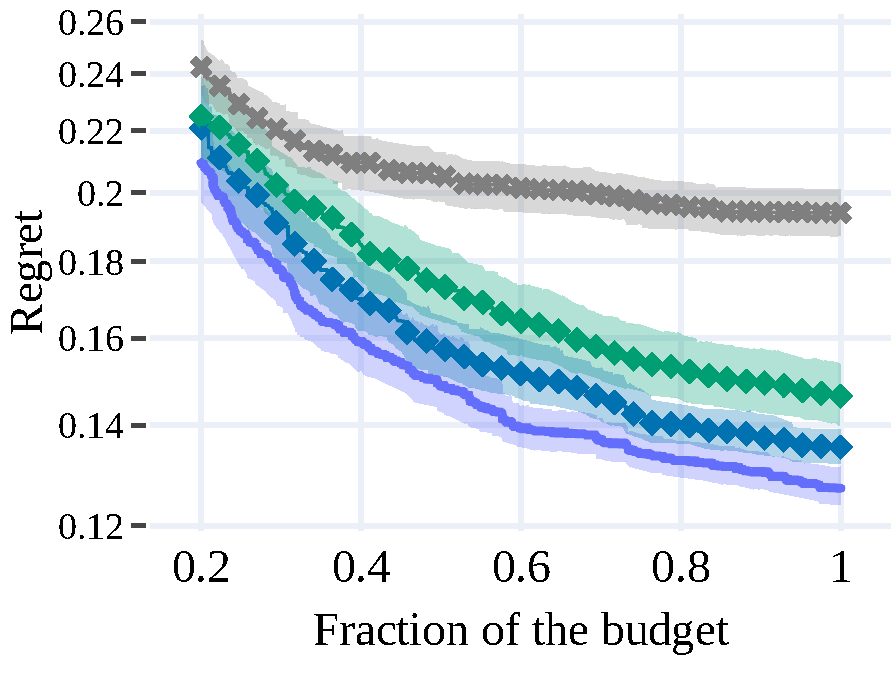
\includegraphics[scale=0.33]{figures/05/figs/figs/co/co_8_init_slcbenchi167168_time.pdf}
        \caption{lcbench 167168}
    \end{subfigure}
\begin{subfigure}[t]{0.32\textwidth}
        \centering
        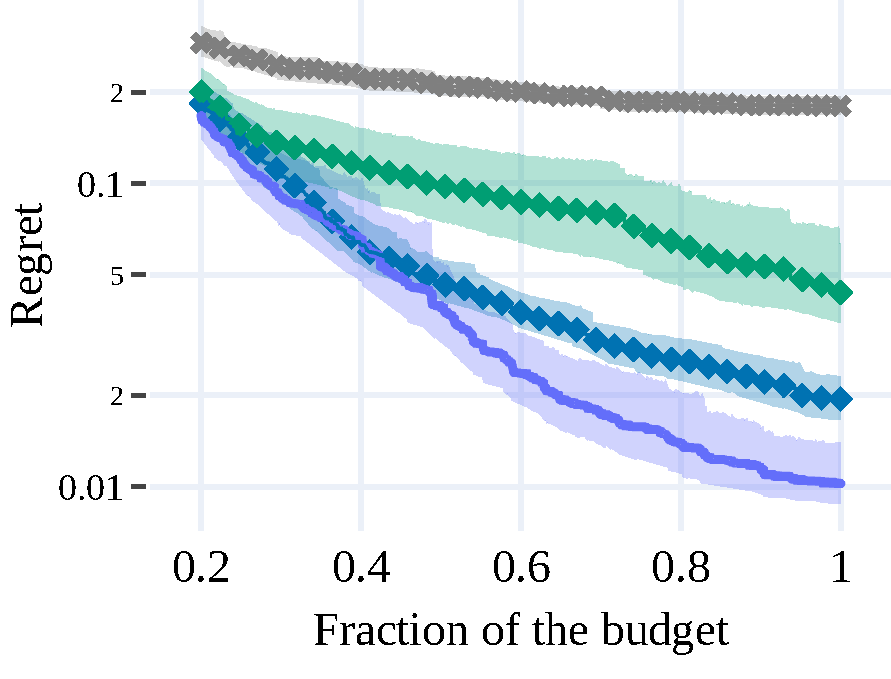
\includegraphics[scale=0.33]{figures/05/figs/figs/co/co_8_init_slcbenchi189873_time.pdf}
        \caption{lcbench 189873}
    \end{subfigure}
\begin{subfigure}[t]{0.32\textwidth}
        \centering
        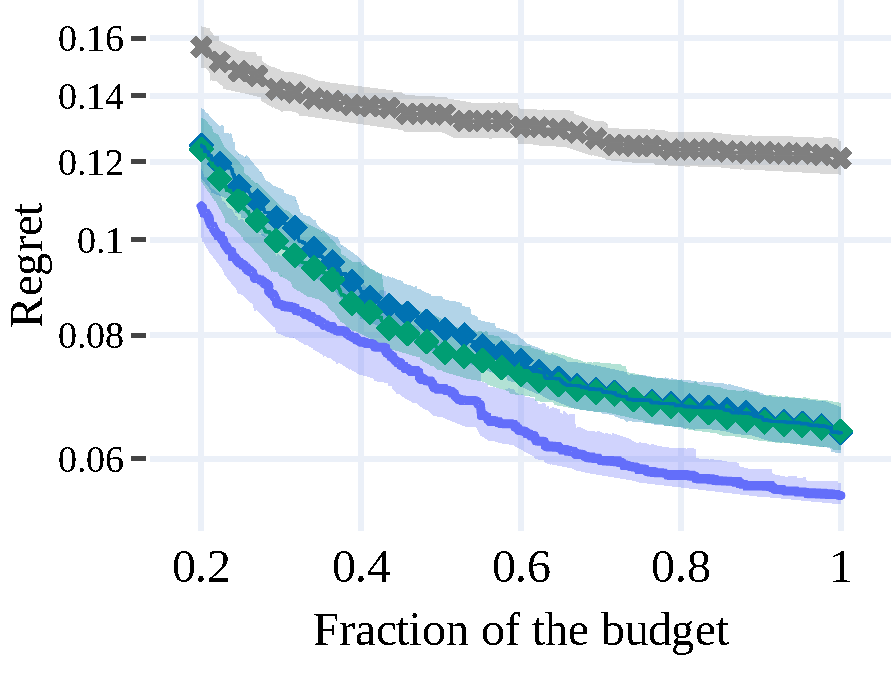
\includegraphics[scale=0.33]{figures/05/figs/figs/co/co_8_init_slcbenchi189906_time.pdf}
        \caption{lcbench 189906}
    \end{subfigure}
\begin{subfigure}[t]{0.32\textwidth}
        \centering
        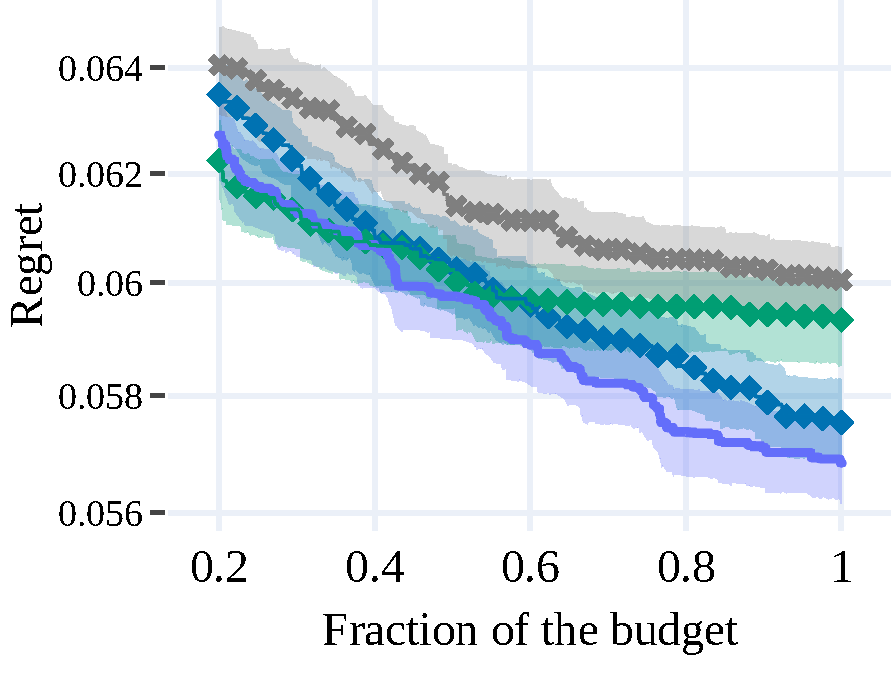
\includegraphics[scale=0.33]{figures/05/figs/figs/co/co_8_init_snb301iCIFAR10_time.pdf}
        \caption{nb301 CIFAR10}
    \end{subfigure}
\begin{subfigure}[t]{0.32\textwidth}
        \centering
        \includegraphics[scale=0.33]{figures/05/figs/figs/co/co_8_init_srbv2\_glmneti375_time.pdf}
        \caption{rbv2\_glmnet 375}
    \end{subfigure}
\begin{subfigure}[t]{0.32\textwidth}
        \centering
        \includegraphics[scale=0.33]{figures/05/figs/figs/co/co_8_init_srbv2\_glmneti458_time.pdf}
        \caption{rbv2\_glmnet 458}
    \end{subfigure}
\begin{subfigure}[t]{0.32\textwidth}
        \centering
        \includegraphics[scale=0.33]{figures/05/figs/figs/co/co_8_init_srbv2\_rangeri16_time.pdf}
        \caption{rbv2\_ranger 16}
    \end{subfigure}
\begin{subfigure}[t]{0.32\textwidth}
        \centering
        \includegraphics[scale=0.33]{figures/05/figs/figs/co/co_8_init_srbv2\_rangeri42_time.pdf}
        \caption{rbv2\_ranger 42}
    \end{subfigure}
\begin{subfigure}[t]{0.32\textwidth}
        \centering
        \includegraphics[scale=0.33]{figures/05/figs/figs/co/co_8_init_srbv2\_rparti14_time.pdf}
        \caption{rbv2\_rpart 14}
    \end{subfigure}


    \begin{subfigure}[t]{1.0\textwidth}
        \centering
        \includegraphics[scale=0.33]{figures/05/figs/figs/co/co_8_init_srbv2\_xgboosti40499_time_legend.pdf}
    \end{subfigure}
    \caption{Convergence plots of \texttt{DyMBO}, HEBO with GP, HEBO with RF, and random search for the YAHPO-SO subset, as a function of the fraction of the wall-clock time budget for each task (continued from~\cref{fig:ch05:full_res}).
    % \er{In the x-axis label, the g of budget is often cut. This actually happens in many other figures too (like Fig. 6)}.
    }
    % \todo{}\er{What's happening in subfigure (t) for HEBO?}}
    \label{fig:ch05:full_res2}
\end{figure*}





\subsection{Running time}
\label{sec:ch05:running_time}

\begin{figure*}[h!]
    \centering
    \begin{subfigure}[t]{0.49\textwidth}
        \centering
        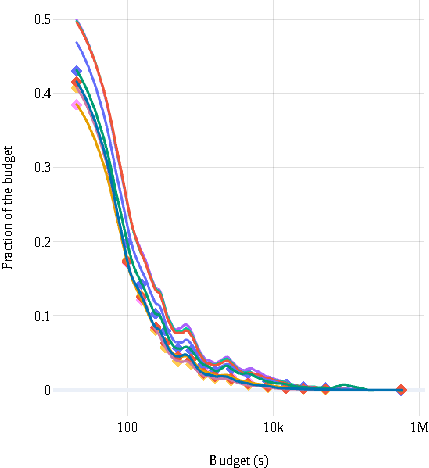
\includegraphics[width=\textwidth]{figures/05/figs/figs/time_percent.pdf}
        \caption{Fraction of budget (in seconds)}
        \label{fig:ch05:rt_frac_of_bud}
    \end{subfigure}
    \begin{subfigure}[t]{0.49\textwidth}
        \centering
        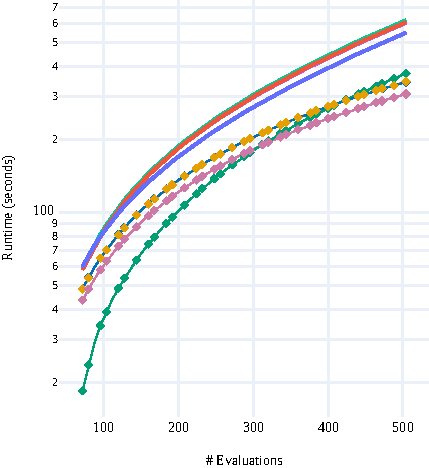
\includegraphics[width=\textwidth]{figures/05/figs/figs/time/nb301_time.pdf}
        \caption{Absolute running time}
        \label{fig:ch05:rt_absolute}
    \end{subfigure}

\includegraphics[width=\textwidth]{figures/05/figs/figs/time/nb301_time_legend.pdf}
    \caption{
    Running time of the optimisation with \texttt{DyMBO} (excluding the time needed to evaluate the target function): (a) as a fraction of optimisation budget, and (b) as absolute running time relative to the number of target function evaluations. Ensembles generally require a higher fraction of the budget compared to single surrogates and take the longest to run in absolute terms, with a notable exception of the ensemble with $\alpha=1.0$, which 
    consumes less budget by an order of magnitude, and which is the fastest to run, due to dynamic pruning. 
    }
    \label{fig:ch05:running-times}
\end{figure*}

We assessed the wall-clock time used by the optimiser itself, \emph{i.e.,} excluding the time required to evaluate the target function, as a percentage of the optimisation budget and as absolute running time relative to the number of target function evaluations. 
\cref{fig:ch05:rt_frac_of_bud} shows the proportion of the optimisation budget (in seconds)
used by the optimiser to suggest the next configurations to sample across all YAHPO Gym functions. 
As expected, for very low budgets (up to approximately 20 seconds), the optimiser consumes a high fraction of the budget (more than 35\%). 
As the budget increases, this fraction decreases, until it becomes negligible (less than 1\% for budgets of more than 10\,000 seconds).
We observe that using ensembles requires a higher fraction of the optimisation budget than using a single surrogate. 
However, the difference becomes indistinguishable when the budget exceeds 1\,000 seconds. 
% When using dynamic ensembling with $\alpha=1.0$, the difference becomes difficult to discern even with a budget of 1\,000 seconds, once more demonstrating the effectiveness of dynamic pruning of surrogate models.

% \hh{minor changes -- check:}
% \changed{
Additionally, we assessed the absolute cost of using different surrogates on the benchmark NAS-Bench-301 from YAHPO Gym, considering up to 512 evaluations. The results are presented in~\cref{fig:ch05:rt_absolute}. 
We first observe that \texttt{DyMBO} 
% \er{It's the second time I find the plural, why? We show one version of DyMBO on that figure.} 
takes the longest to run, although the gap from the single-surrogate HEBO variants is not large, at around 150 seconds for 512 evaluations; this is a relatively short time given that each evaluation of the target function takes around one hour. For lower numbers of evaluations, the gap is even smaller.
% We also notice that ensembling approaches take roughly twice as long as tree-based surrogates. 
GPs are the fastest to run with a low number of evaluations, however the gap between them and tree-based methods shrinks substantially as more observations are added.
% }



\subsection{Evolution of weights}
\label{sec:ch05:weights}

We show the evolution of the weights of the surrogate models in the ensemble over the course of the optimisation in~\cref{fig:ch05:weights}. 
To this end, we made use of the data from the experiment with fixed 512 evaluations as described in~\cref{sec:ch05:diff_exp_setup}, with GP and RF as surrogate models.
% We show the results in. 
% \changed{
We observe that the weights of the surrogates change rapidly and frequently during the optimisation process, \emph{i.e.}, the weights are not constant, and the surrogates are not used equally. 
This indicates that neither surrogate consistently dominates 
and that the relative predictive performance of GP and RF alternates across iterations.
This switching behaviour justifies the use of a dynamic ensemble over simply choosing a single surrogate model at the start of optimisation.

We also see different weight dynamics, depending on the given target function. 
% \hh{better: optimised? or ... on the given target function?}.
On some target functions, \emph{e.g.,}~\cref{fig:ch05:weights}(c, p, q), GP is assigned a near-constant weight of $1$ for the majority of the optimisation process, suggesting a strong and 
stable preference for GP on these problems.
On the target function in~\cref{fig:ch05:weights}(n), it is RF that consistently dominates the optimisation with a near-constant weight of $1$.
In contrast, on most other target functions, the weights oscillate frequently between the two surrogates, indicating that both GP and RF contribute meaningfully and that neither is uniformly superior.
Furthermore, the onset of switching behaviour varies substantially depending on the target function.
% }
% \todo{Could the authors kindly add their insight(s) that the reader could take away from Figure 18?}
% }
\begin{figure*}
    \centering
    \begin{subfigure}[t]{0.24\textwidth}
        \centering
        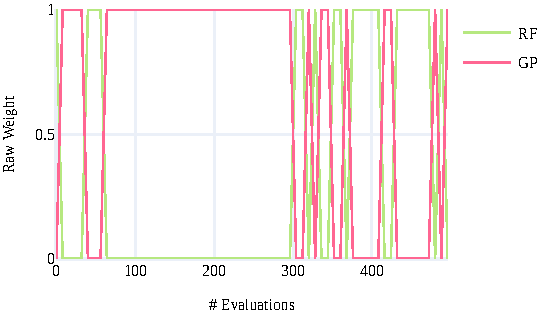
\includegraphics[width=\textwidth]{figures/05/figs/figs/weights/w_2d_init_slcbenchi167168_smens_ranking_loss_rf_gp_init_orf_eval_all.pdf}
        \caption{lcbench 167168}
    \end{subfigure}
\begin{subfigure}[t]{0.24\textwidth}
        \centering
        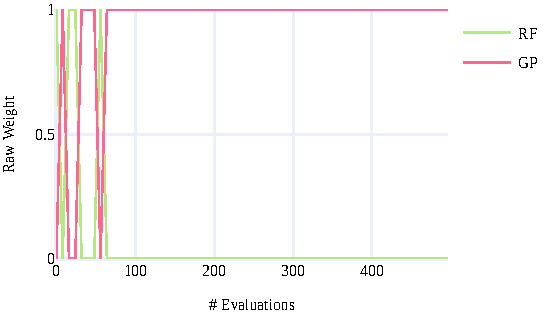
\includegraphics[width=\textwidth]{figures/05/figs/figs/weights/w_2d_init_slcbenchi189873_smens_ranking_loss_rf_gp_init_orf_eval_all.pdf}
        \caption{lcbench 189873}
    \end{subfigure}
\begin{subfigure}[t]{0.24\textwidth}
        \centering
        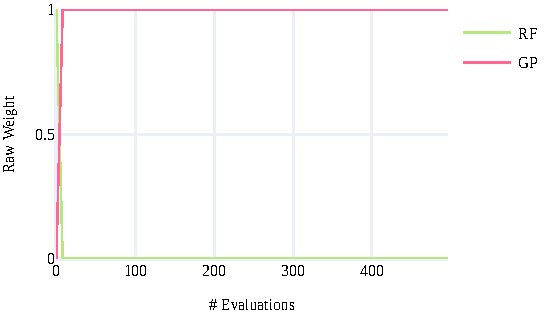
\includegraphics[width=\textwidth]{figures/05/figs/figs/weights/w_2d_init_slcbenchi189906_smens_ranking_loss_rf_gp_init_orf_eval_all.pdf}
        \caption{lcbench 189906}
    \end{subfigure}
\begin{subfigure}[t]{0.24\textwidth}
        \centering
        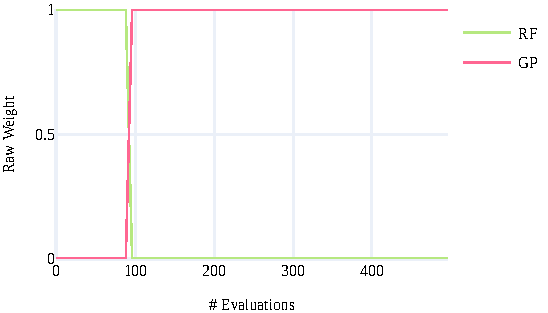
\includegraphics[width=\textwidth]{figures/05/figs/figs/weights/w_2d_init_snb301iCIFAR10_smens_ranking_loss_rf_gp_init_orf_eval_all.pdf}
        \caption{nb301 CIFAR10}
    \end{subfigure}
\begin{subfigure}[t]{0.24\textwidth}
        \centering
        \includegraphics[width=\textwidth]{figures/05/figs/figs/weights/w_2d_init_srbv2\_glmneti375_smens_ranking_loss_rf_gp_init_orf_eval_all.pdf}
        \caption{rbv2\_glmnet 375}
    \end{subfigure}
\begin{subfigure}[t]{0.24\textwidth}
        \centering
        \includegraphics[width=\textwidth]{figures/05/figs/figs/weights/w_2d_init_srbv2\_glmneti458_smens_ranking_loss_rf_gp_init_orf_eval_all.pdf}
        \caption{rbv2\_glmnet 458}
    \end{subfigure}
\begin{subfigure}[t]{0.24\textwidth}
        \centering
        \includegraphics[width=\textwidth]{figures/05/figs/figs/weights/w_2d_init_srbv2\_rangeri16_smens_ranking_loss_rf_gp_init_orf_eval_all.pdf}
        \caption{rbv2\_ranger 16}
    \end{subfigure}
\begin{subfigure}[t]{0.24\textwidth}
        \centering
        \includegraphics[width=\textwidth]{figures/05/figs/figs/weights/w_2d_init_srbv2\_rangeri42_smens_ranking_loss_rf_gp_init_orf_eval_all.pdf}
        \caption{rbv2\_ranger 42}
    \end{subfigure}
\begin{subfigure}[t]{0.24\textwidth}
        \centering
        \includegraphics[width=\textwidth]{figures/05/figs/figs/weights/w_2d_init_srbv2\_rparti14_smens_ranking_loss_rf_gp_init_orf_eval_all.pdf}
        \caption{rbv2\_rpart 14}
    \end{subfigure}
\begin{subfigure}[t]{0.24\textwidth}
        \centering
        \includegraphics[width=\textwidth]{figures/05/figs/figs/weights/w_2d_init_srbv2\_rparti40499_smens_ranking_loss_rf_gp_init_orf_eval_all.pdf}
        \caption{rbv2\_rpart 40499}
    \end{subfigure}
\begin{subfigure}[t]{0.24\textwidth}
        \centering
        \includegraphics[width=\textwidth]{figures/05/figs/figs/weights/w_2d_init_srbv2\_superi1053_smens_ranking_loss_rf_gp_init_orf_eval_all.pdf}
        \caption{rbv2\_super 1053}
    \end{subfigure}
\begin{subfigure}[t]{0.24\textwidth}
        \centering
        \includegraphics[width=\textwidth]{figures/05/figs/figs/weights/w_2d_init_srbv2\_superi1457_smens_ranking_loss_rf_gp_init_orf_eval_all.pdf}
        \caption{rbv2\_super 1457}
    \end{subfigure}
\begin{subfigure}[t]{0.24\textwidth}
        \centering
        \includegraphics[width=\textwidth]{figures/05/figs/figs/weights/w_2d_init_srbv2\_superi1063_smens_ranking_loss_rf_gp_init_orf_eval_all.pdf}
        \caption{rbv2\_super 1063}
    \end{subfigure}
\begin{subfigure}[t]{0.24\textwidth}
        \centering
        \includegraphics[width=\textwidth]{figures/05/figs/figs/weights/w_2d_init_srbv2\_superi1479_smens_ranking_loss_rf_gp_init_orf_eval_all.pdf}
        \caption{rbv2\_super 1479}
    \end{subfigure}
\begin{subfigure}[t]{0.24\textwidth}
        \centering
        \includegraphics[width=\textwidth]{figures/05/figs/figs/weights/w_2d_init_srbv2\_superi15_smens_ranking_loss_rf_gp_init_orf_eval_all.pdf}
        \caption{rbv2\_super 15}
    \end{subfigure}
\begin{subfigure}[t]{0.24\textwidth}
        \centering
        \includegraphics[width=\textwidth]{figures/05/figs/figs/weights/w_2d_init_srbv2\_superi1468_smens_ranking_loss_rf_gp_init_orf_eval_all.pdf}
        \caption{rbv2\_super 1468}
    \end{subfigure}
\begin{subfigure}[t]{0.24\textwidth}
        \centering
        \includegraphics[width=\textwidth]{figures/05/figs/figs/weights/w_2d_init_srbv2\_xgboosti12_smens_ranking_loss_rf_gp_init_orf_eval_all.pdf}
        \caption{rbv2\_xgboost 12}
    \end{subfigure}
\begin{subfigure}[t]{0.24\textwidth}
        \centering
        \includegraphics[width=\textwidth]{figures/05/figs/figs/weights/w_2d_init_srbv2\_xgboosti1501_smens_ranking_loss_rf_gp_init_orf_eval_all.pdf}
        \caption{rbv2\_xgboost 1501}
    \end{subfigure}
\begin{subfigure}[t]{0.24\textwidth}
        \centering
        \includegraphics[width=\textwidth]{figures/05/figs/figs/weights/w_2d_init_srbv2\_xgboosti16_smens_ranking_loss_rf_gp_init_orf_eval_all.pdf}
        \caption{rbv2\_xgboost 16}
    \end{subfigure}
\begin{subfigure}[t]{0.24\textwidth}
        \centering
        \includegraphics[width=\textwidth]{figures/05/figs/figs/weights/w_2d_init_srbv2\_xgboosti40499_smens_ranking_loss_rf_gp_init_orf_eval_all.pdf}
        \caption{rbv2\_xgboost 40499}
    \end{subfigure}

    \caption{Weights of the models in the \texttt{DyMBO} surrogate ensemble on the first seed of each of the YAHPO-SO target functions as a function of the number of evaluations for each task. Different target functions have different weights for the models.}
    % \er{Why do we exclude ET and GB from this analysis?}}
    \label{fig:ch05:weights}
\end{figure*}


\subsection{Surrogate model accuracy}
\label{sec:ch05:surr-acc}

% \changed{
To analyse why dynamic surrogate tailoring yields superior performance, we assessed the predictive quality of the surrogate models used in the ensemble themselves.
The results can be seen in~\cref{fig:ch05:surrogate-accuracy}, where we compare the ranking loss achieved by \texttt{DyMBO} with different $\alpha$ values and single-surrogate models on a set of 256 randomly sampled configurations. 
We see that all \texttt{DyMBO} variants achieve lower ranking loss than single surrogates.
In particular, \texttt{DyMBO} variants with lower $\alpha$ values achieve better ranking loss, while the performance observed in previous sections indicated that higher values of $\alpha$ are better.
We furthermore looked into the pairwise distance between the sampled points, which we measure as Gower's distance between the newly proposed configurations in each batch and the incumbent. We found that higher $\alpha$ values result in higher pairwise distances (0.0606 for $\alpha=1.0$, 0.0578 for $\alpha=0.9$, 0.0544 for $\alpha=0.5$ and 0.0496 for $\alpha=0.1$), \emph{i.e.}, more diverse sampling, shows enhanced exploration. This is due to the more aggressive selection policy.

% \todo{fix according to the comment by reviewer 2} 
% However, the variants with lower $\alpha$ values result in worse overall performance since the total budget is dictated by the time, and, as observed in~\autoref{sec:running_time}, the running times of the lower-$\alpha$ variants of \texttt{DyMBO} is higher. 
% Therefore, we expose a trade-off between model accuracy and running time, in which \texttt{DyMBO} variants with $\alpha=1.0$ and $\alpha=0.9$ perform very well. 
% \changed{
% Therefore, we expose an apparent trade-off between surrogate accuracy (as measured by ranking loss) and running time.
% We note that our experiment under the fixed-evaluation budget in~\autoref{sec:diff_exp_setup} also ranks higher-$\alpha$ \texttt{DyMBO} variants above lower-$\alpha$ variants, suggesting the effect is not purely an artefact of the running time.
% A direct comparison of ranking loss and downstream performance under the fixed-evaluation budget remains an important direction for confirming this observation more rigorously, but is left for future work.
% \changed{
% However, we note that our experiment under the fixed-evaluation budget in~\autoref{sec:diff_exp_setup} ranks higher-$\alpha$ \texttt{DyMBO} variants above lower-$\alpha$ variants, suggesting that performance is not heavily influenced by the predictive quality of the surrogate models used in the ensemble. One may attribute this behaviour to the more conservative nature of the ensembling strategy for low values of $\alpha$, which limits the explorative capabilities of the BO algorithm, often proven to be beneficial [reference].
% }
% A direct comparison of ranking loss and downstream performance under the fixed-evaluation budget remains an important direction for confirming this observation more rigorously, but is left for future work.
% }
% }

\begin{figure}
    \centering
    \begin{subfigure}{0.49\textwidth}
        \centering
        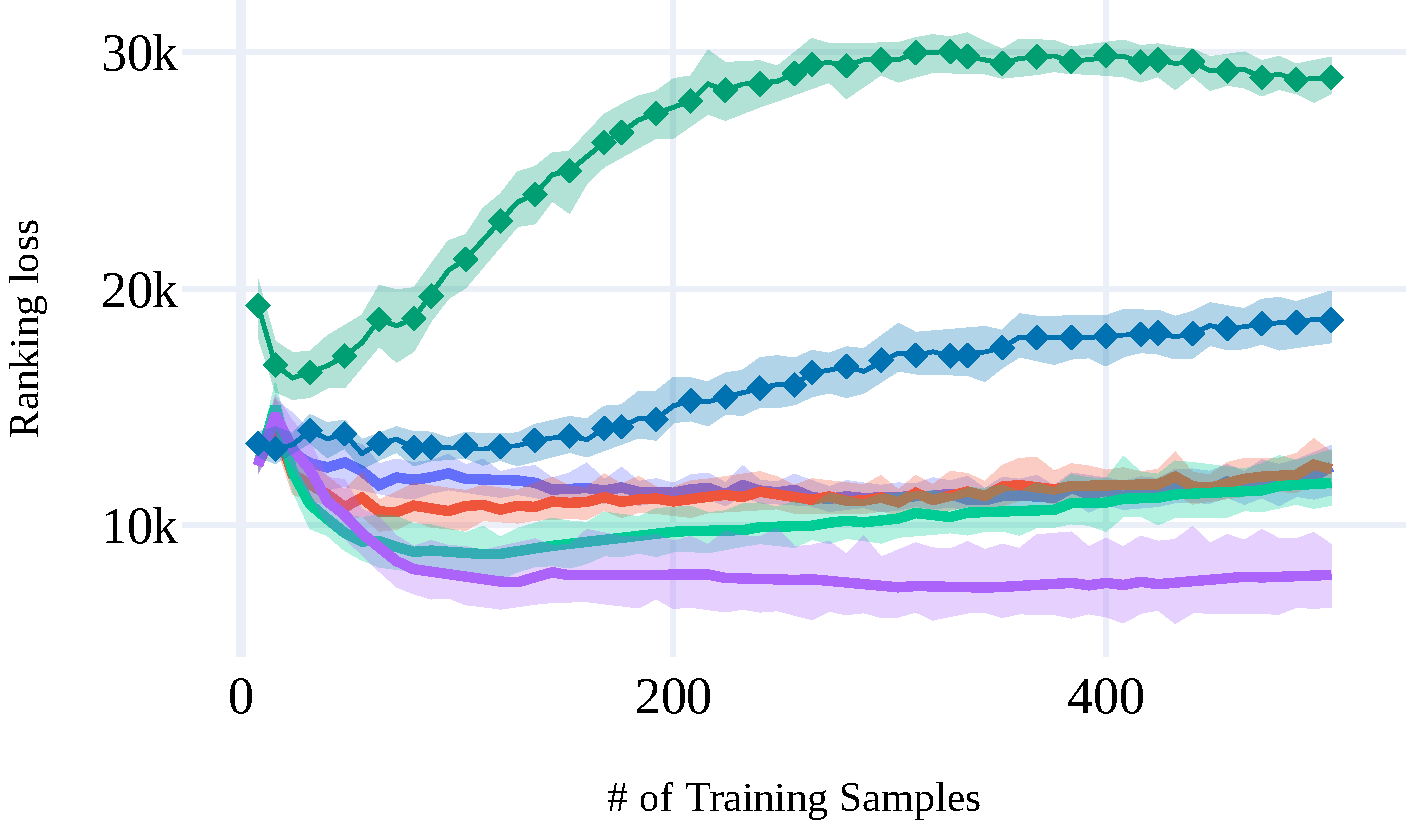
\includegraphics[scale=0.33]{figures/05/figs/figs/model_acc.pdf}
        \caption{All}
    \end{subfigure}
    \begin{subfigure}{0.49\textwidth}
        \centering
        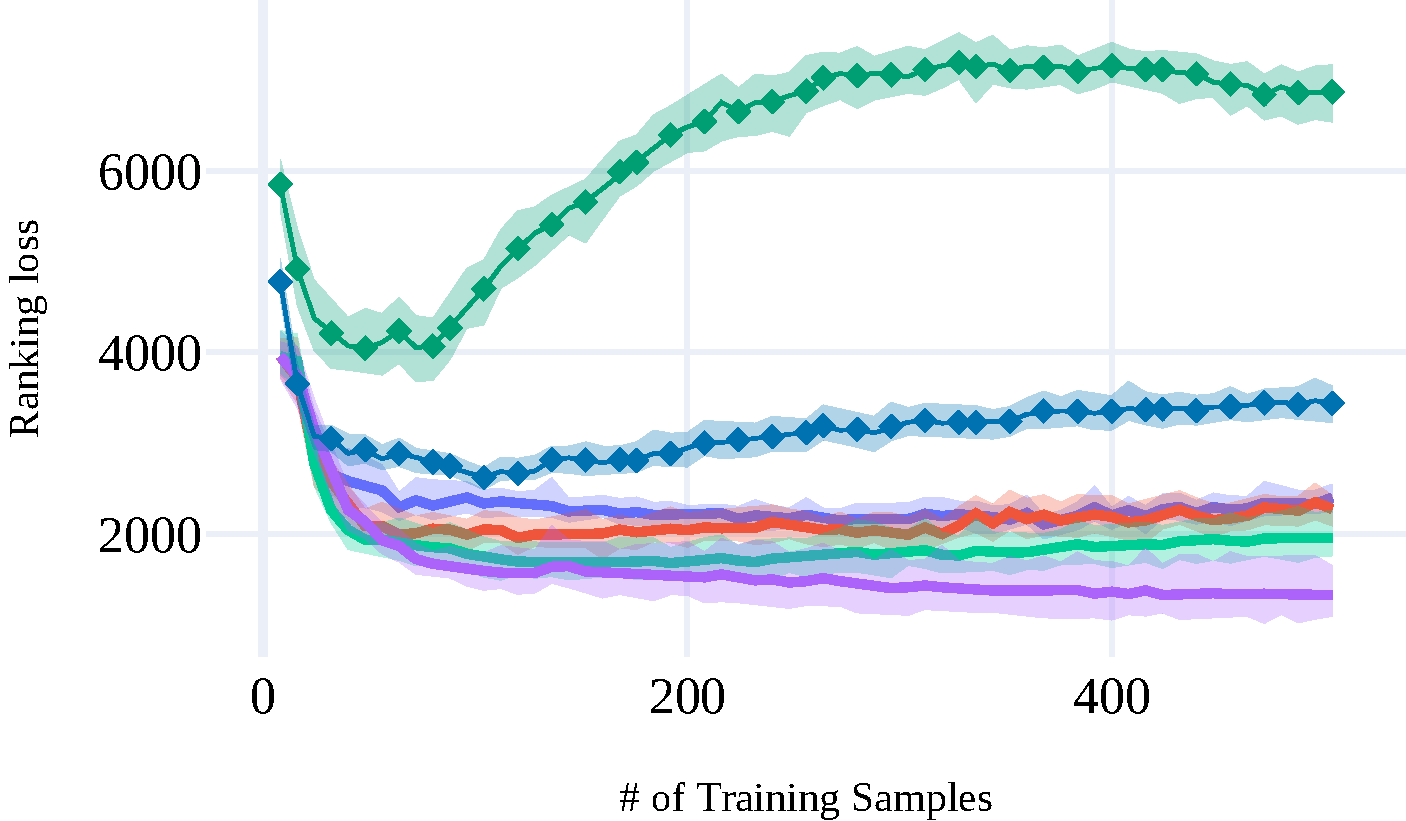
\includegraphics[scale=0.33]{figures/05/figs/figs/model_acc_best50.pdf}
        \caption{Top 50\%}
    \end{subfigure}
    \begin{subfigure}{0.49\textwidth}
        \centering
        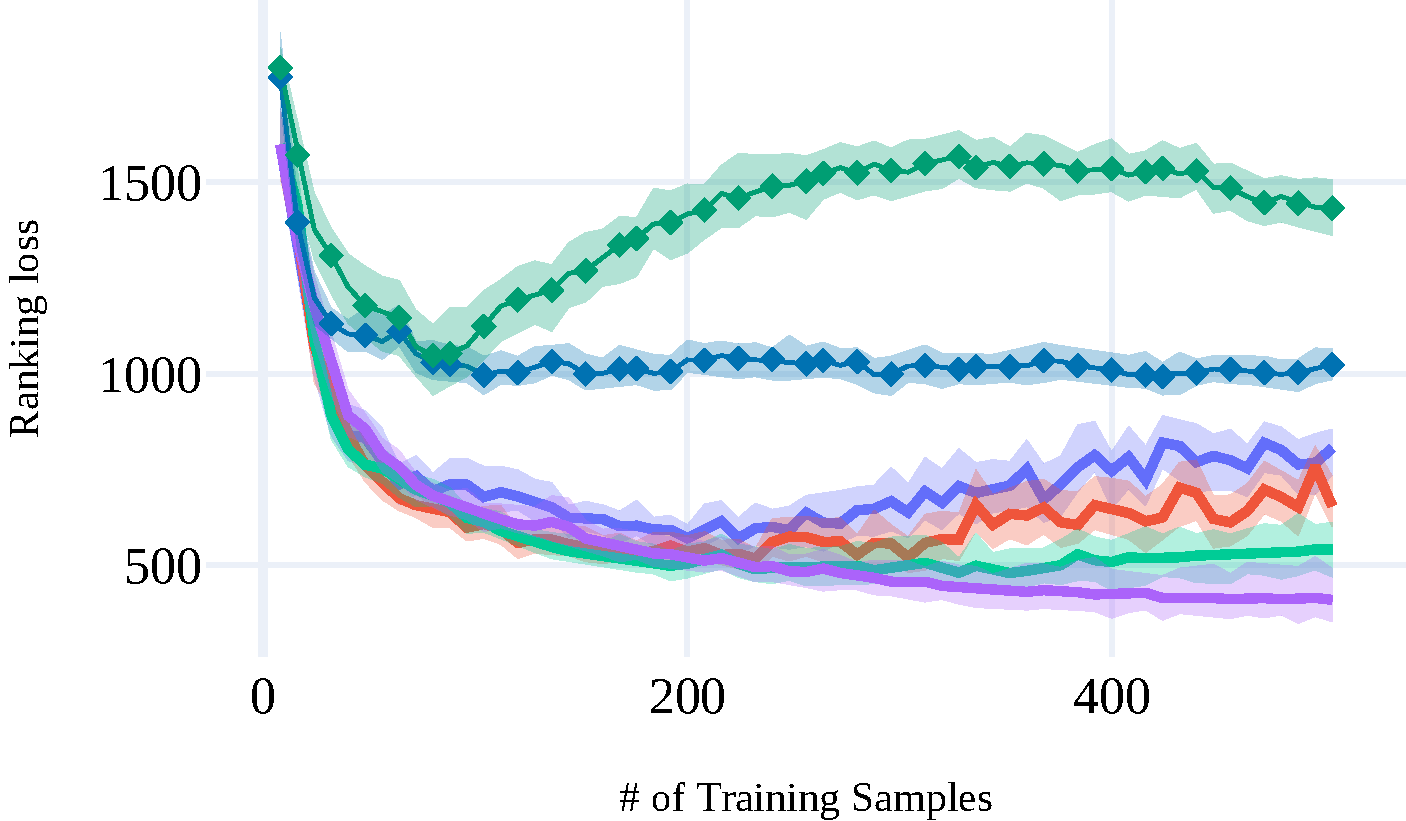
\includegraphics[scale=0.33]{figures/05/figs/figs/model_acc_best25.pdf}
        \caption{Top 25\%}
    \end{subfigure}
    \begin{subfigure}{0.49\textwidth}
        \centering
        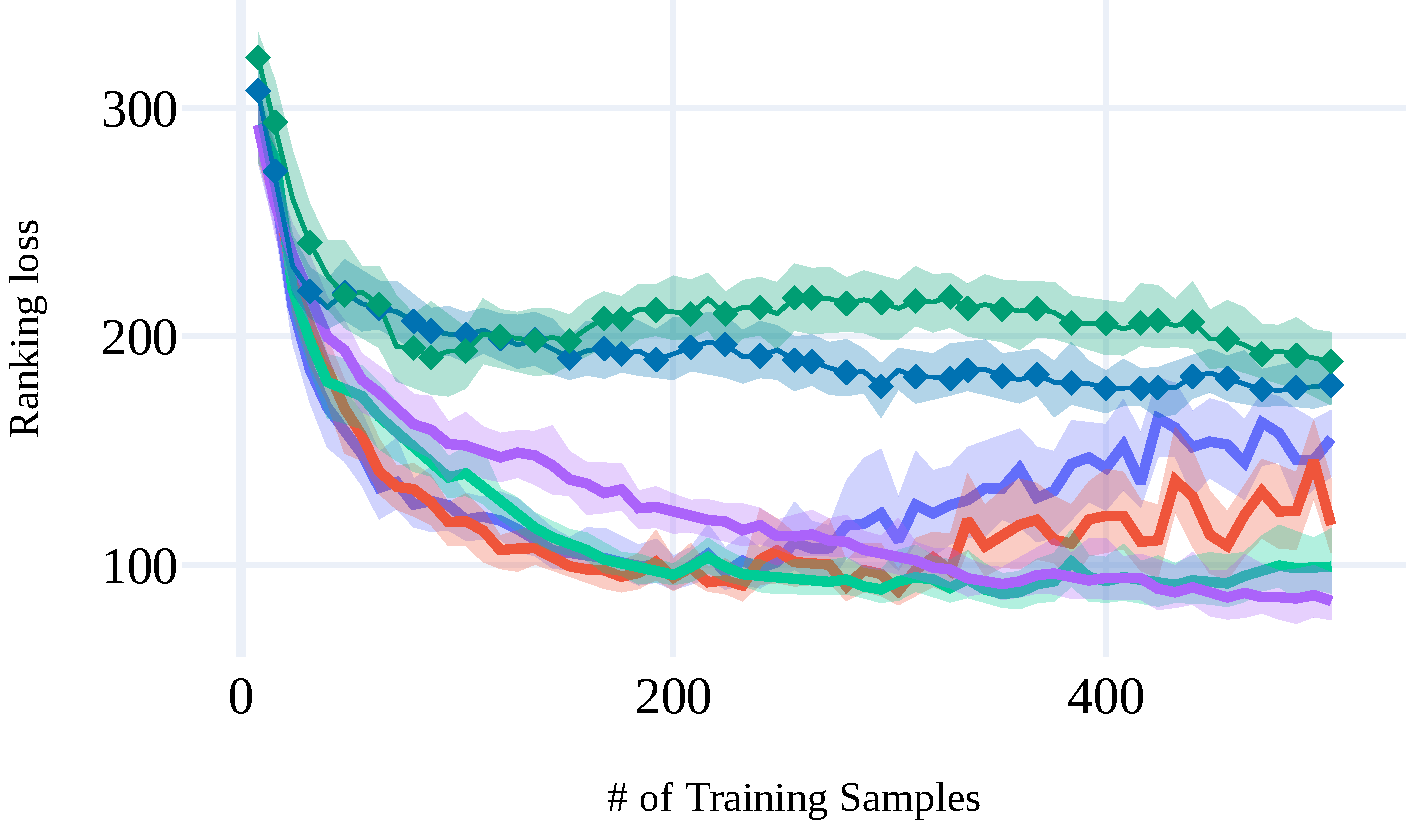
\includegraphics[scale=0.33]{figures/05/figs/figs/model_acc_best10.pdf}
        \caption{Top 10\%}
    \end{subfigure}
    
    
\includegraphics[scale=0.33]{figures/05/figs/figs/model_acc_legend.pdf}
    \caption{Ranking loss as a measure of surrogate accuracy of \texttt{DyMBO} (with different values of $\alpha$) and single-surrogate HEBO variants with RF and GP. The ranking loss is measured on randomly sampled configurations: (a) ranking on all configurations; (b) ranking on the top 50\% of configurations; (c) ranking on the top 25\% of configurations; and (d) ranking on the top 10\% of configurations. All \texttt{DyMBO} variants exhibit substantially better ranking loss than single-surrogate baselines. 
    }
    \label{fig:ch05:surrogate-accuracy}
\end{figure}



\section{Additional baselines}
\label{sec:ch05:add_baselines}

We describe additional baselines against which we compared our method. We note that these baselines are described in the appendix and not in the main paper as they are either not an established HPO method or not compatible with some of the benchmarks.

\paragraph{HEBO with different surrogate models.} To isolate the effect of the surrogate model, we evaluated four single-surrogate HEBO variants using GP, RF, ET, and GB, respectively. All other components of the optimisation pipeline, including the initial-design strategy, acquisition function, and acquisition-function optimiser, were kept unchanged. \cref{fig:ch05:gen_res_more_surrogate} compares these variants with \texttt{DyMBO} ($\alpha=1.0$) and random search. The relative performance of the single-surrogate variants varies with the cost of the target function: GP performs particularly well on cheap and medium-cost functions, whereas RF becomes the strongest single-surrogate baseline on expensive functions toward the end of the optimisation. ET and GB generally obtain lower ranks, although their relative performance also changes across budget groups. \texttt{DyMBO} achieves the best mean rank in every group, demonstrating the benefit of dynamically selecting between complementary surrogate models instead of committing to a single model before optimisation.

\begin{figure*}[h]
    \centering
    \begin{subfigure}[t]{0.49\textwidth}
        \centering
        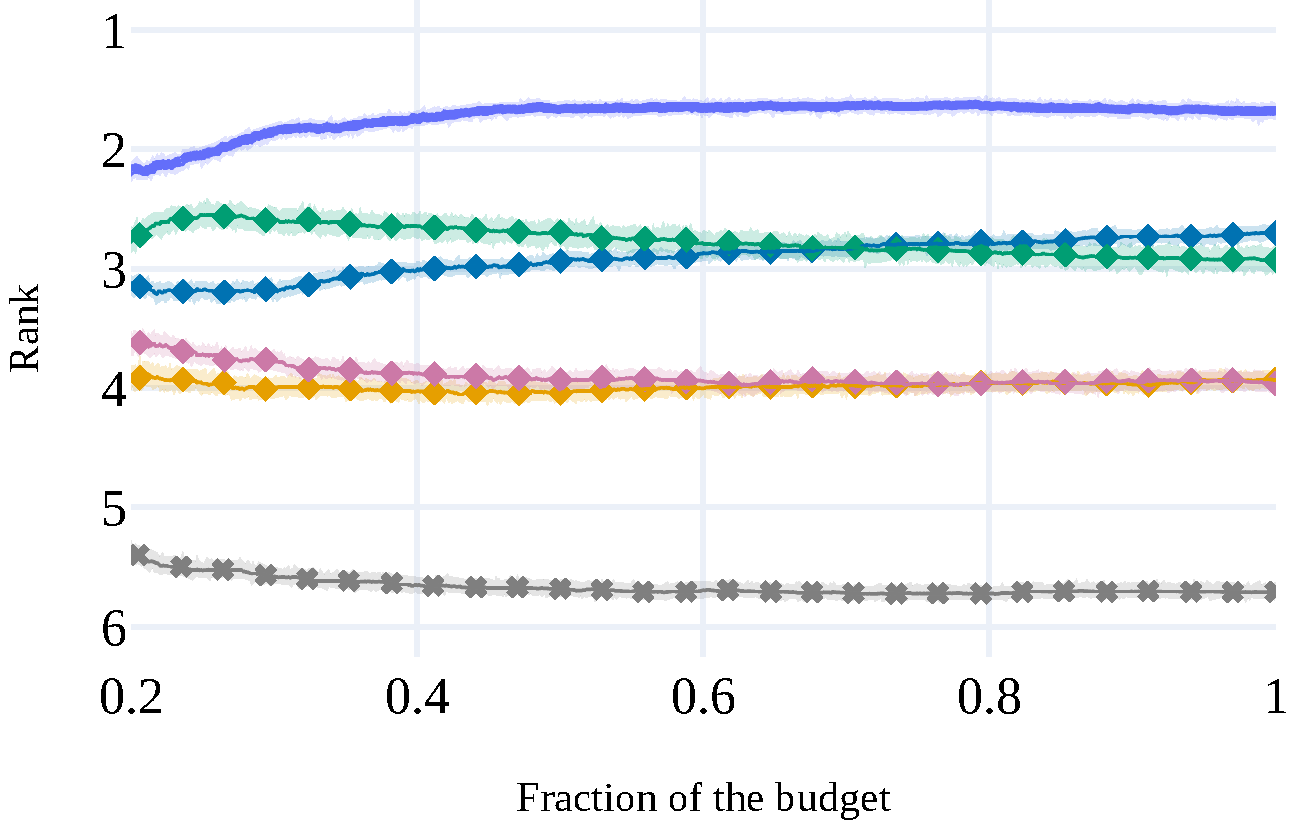
\includegraphics[scale=0.33]{figures/05/figs/figs/ranks/main_ranks_all_surrogates2_all.pdf}
        \caption{All target functions}
    \end{subfigure}
    \begin{subfigure}[t]{0.49\textwidth}
        \centering
        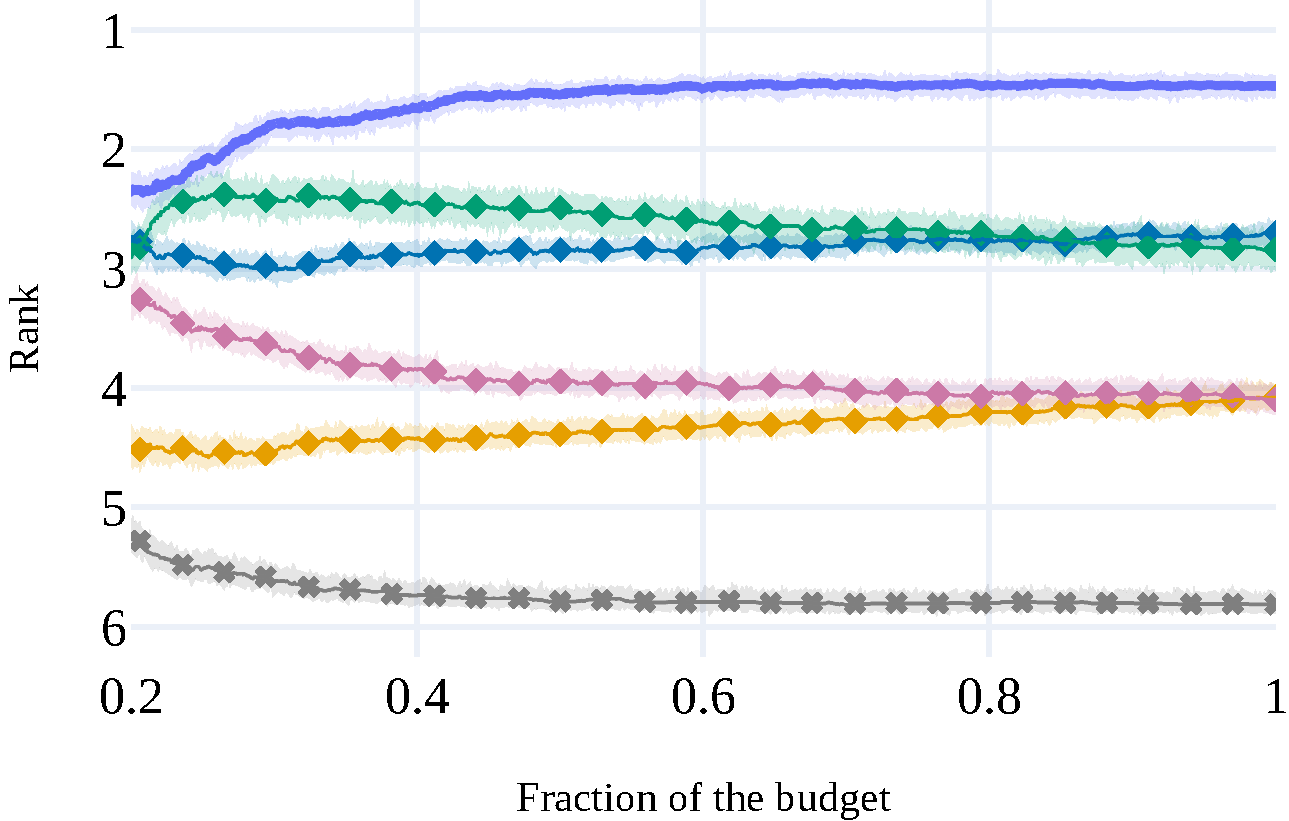
\includegraphics[scale=0.33]{figures/05/figs/figs/ranks/main_ranks_all_surrogates2_cheap.pdf}
        \caption{Cheap (up to 10 minutes)}
    \end{subfigure}
    \begin{subfigure}[t]{0.49\textwidth}
        \centering
        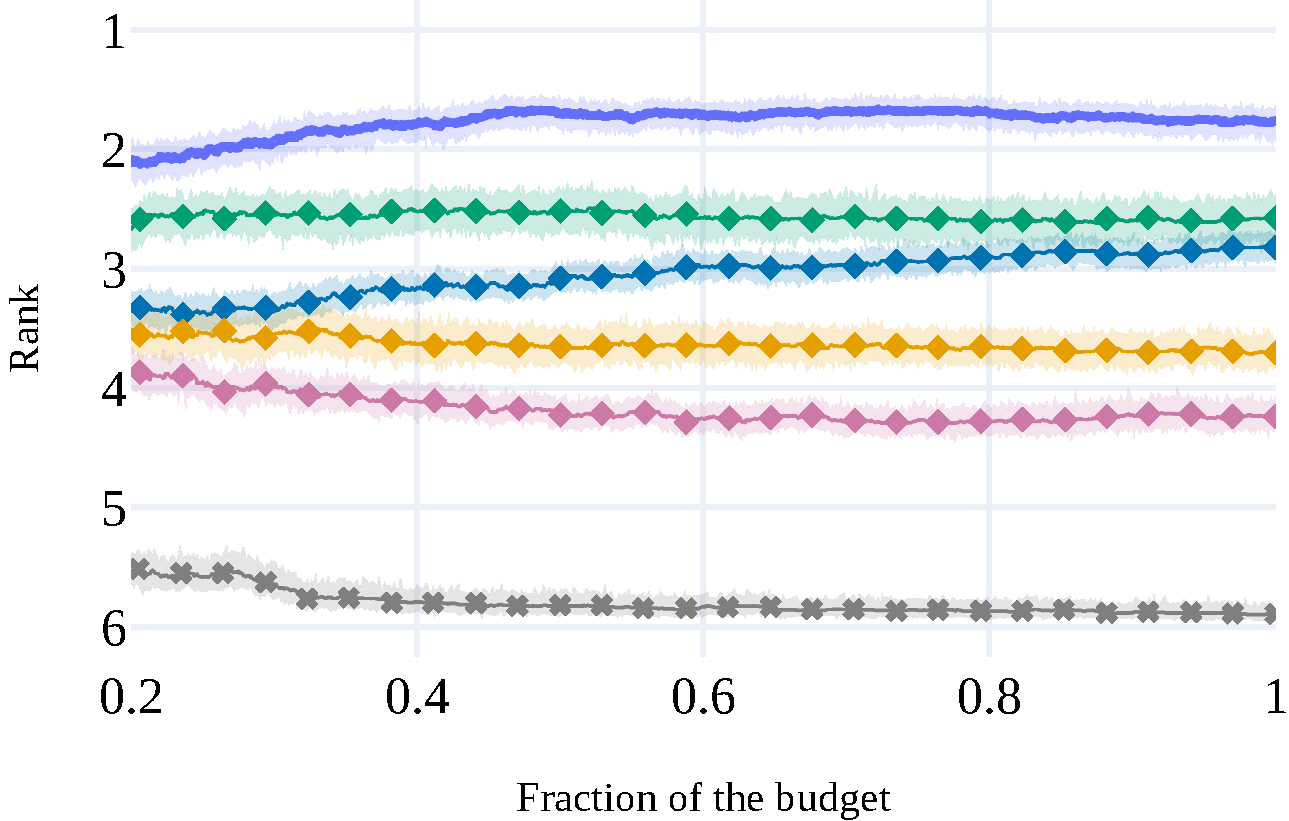
\includegraphics[scale=0.33]{figures/05/figs/figs/ranks/main_ranks_all_surrogates2_medium.pdf}
        \caption{Medium-cost (more than 10 minutes, up to \mbox{1 hour})}
    \end{subfigure}
    \begin{subfigure}[t]{0.49\textwidth}
        \centering
        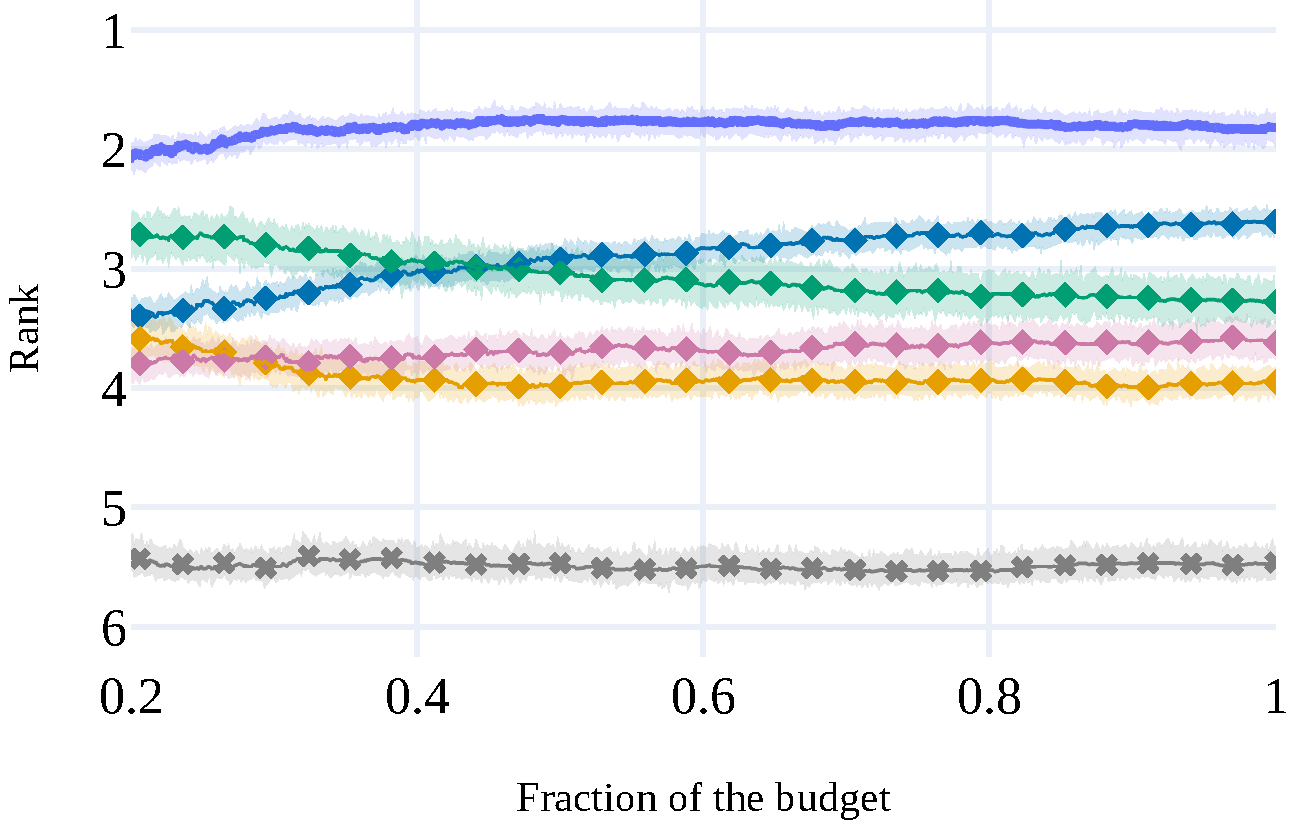
\includegraphics[scale=0.33]{figures/05/figs/figs/ranks/main_ranks_all_surrogates2_expensive.pdf}
        \caption{Expensive (more than 1 hour)}
    \end{subfigure}
    \begin{subfigure}[t]{\textwidth}
        \centering
        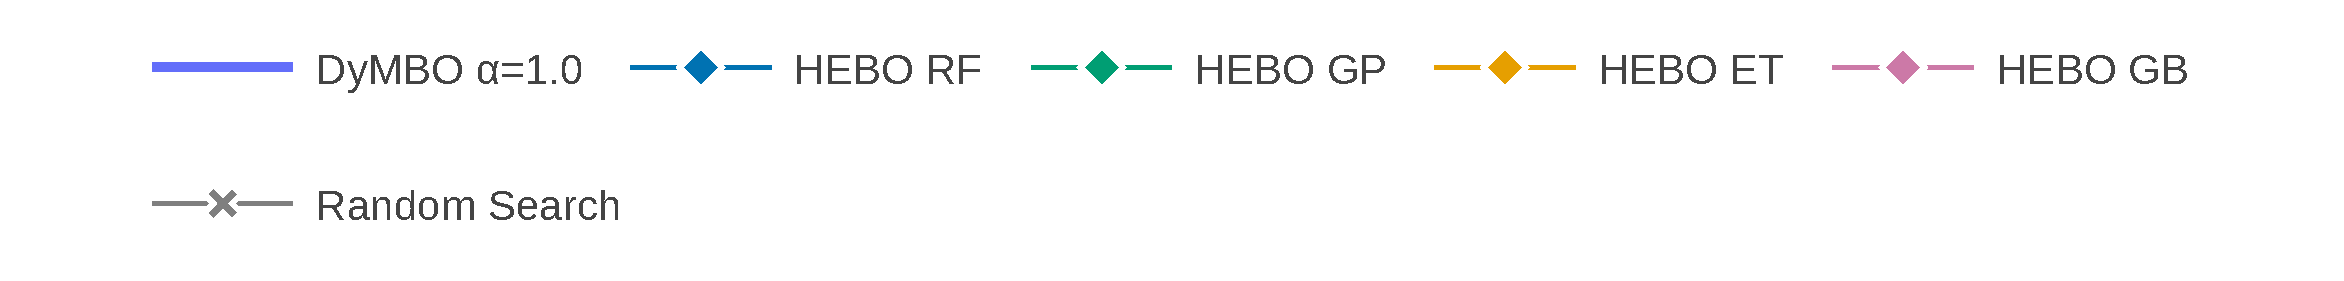
\includegraphics[scale=0.33]{figures/05/figs/figs/ranks/main_ranks_all_surrogates2_all_legend.pdf}
    \end{subfigure}
    \caption{
    Mean rank of DyMBO with $\alpha=1.0$, single-surrogate HEBO variants using RF, GP, ET, or GB, and random search on YAHPO Gym and JAHS-Bench-201 as a function of the fraction of the wall-clock time budget for each task. Results are shown for (a) all target functions, (b) cheap functions with budgets of up to 10 minutes, (c) medium-cost functions with budgets between 10 minutes and 1 hour, and (d) expensive functions with budgets exceeding 1 hour. Smaller numbers indicate a better rank, thus better performance. \texttt{DyMBO} achieves the best mean rank in every budget group, while the relative performance of the individual surrogate models varies with target function cost.
    }
    \label{fig:ch05:gen_res_more_surrogate}
\end{figure*}

\paragraph{Squirrel.}
Squirrel~\citep{AwaEtAl20} is an HPO method which won the third place in the NeurIPS black-box optimisation challenge. 
Squirrel uses a GP surrogate model and a portfolio of acquisition functions, including EI, PI, Lower Confidence Bound (LCB)~\citep{ForEtAl08} and logEI~\citep{HutEtAl11}, selected adaptively during optimisation.
It should be noted that Squirrel was specifically designed to meet the rules of the challenge (batch size, number of random samples, total number of batches). A similar approach is Optuna AutoSampler, which selects the HPO method to use based on hand-crafted rules. We ran Squirrel only on the YAHPO Gym benchmark, as it is not compatible with JAHS-Bench-201 due to Python package versioning. We provide the results in \cref{fig:ch05:squirrel}, where we see that our approach outperforms Squirrel on almost all benchmarks (mean rank of 1.07).


\begin{figure*}
    \centering
    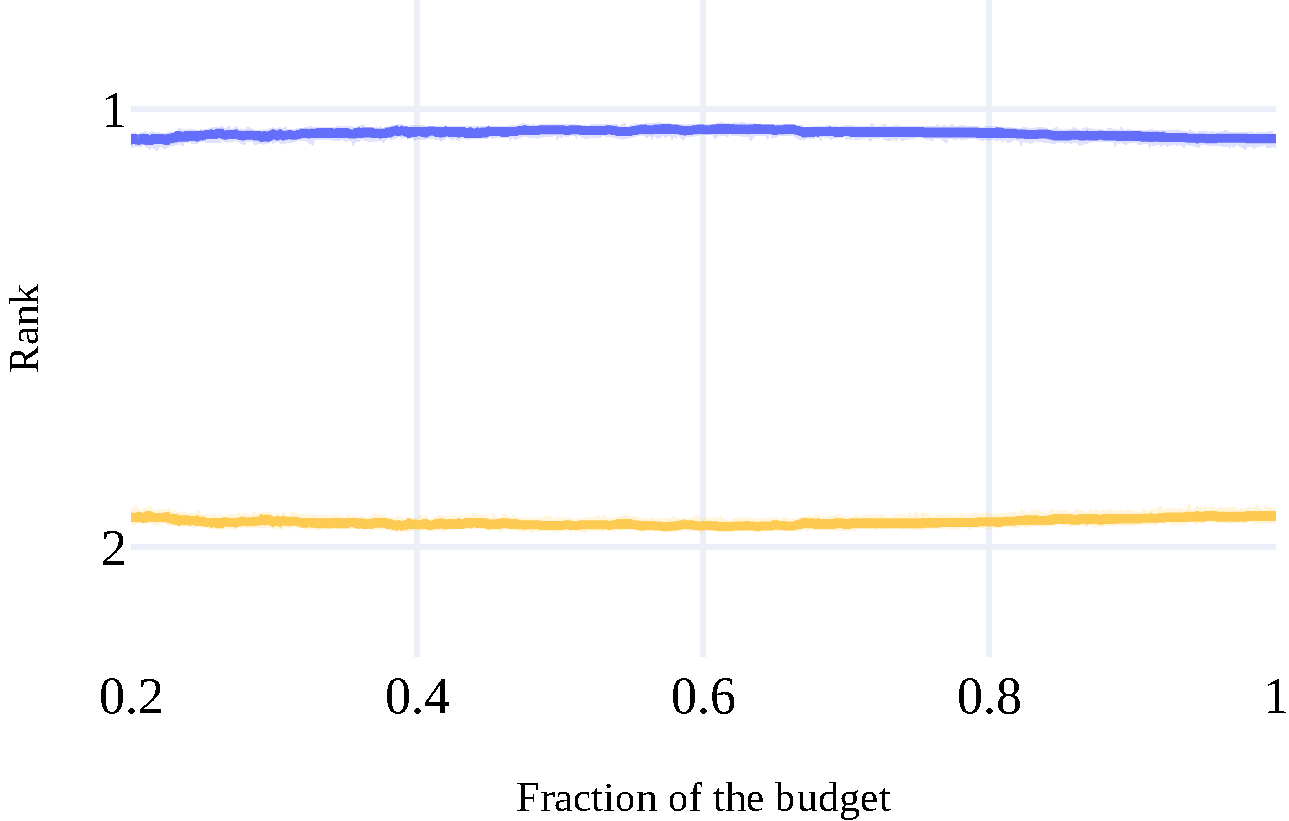
\includegraphics[scale=0.33]{figures/05/figs/figs/ranks/additional_baselines_squirrel_all.pdf}
    
\includegraphics[scale=0.33]{figures/05/figs/figs/ranks/additional_baselines_squirrel_all_legend.pdf}
    \caption{Comparison of \texttt{DyMBO} to Squirrel as a function of the fraction of the wall-clock time budget on YAHPO Gym. Our method outperforms Squirrel on almost all benchmarks. 
    }
    \label{fig:ch05:squirrel}

\end{figure*}

\begin{figure*}
    \centering
    \begin{subfigure}[t]{\textwidth}
    \centering
    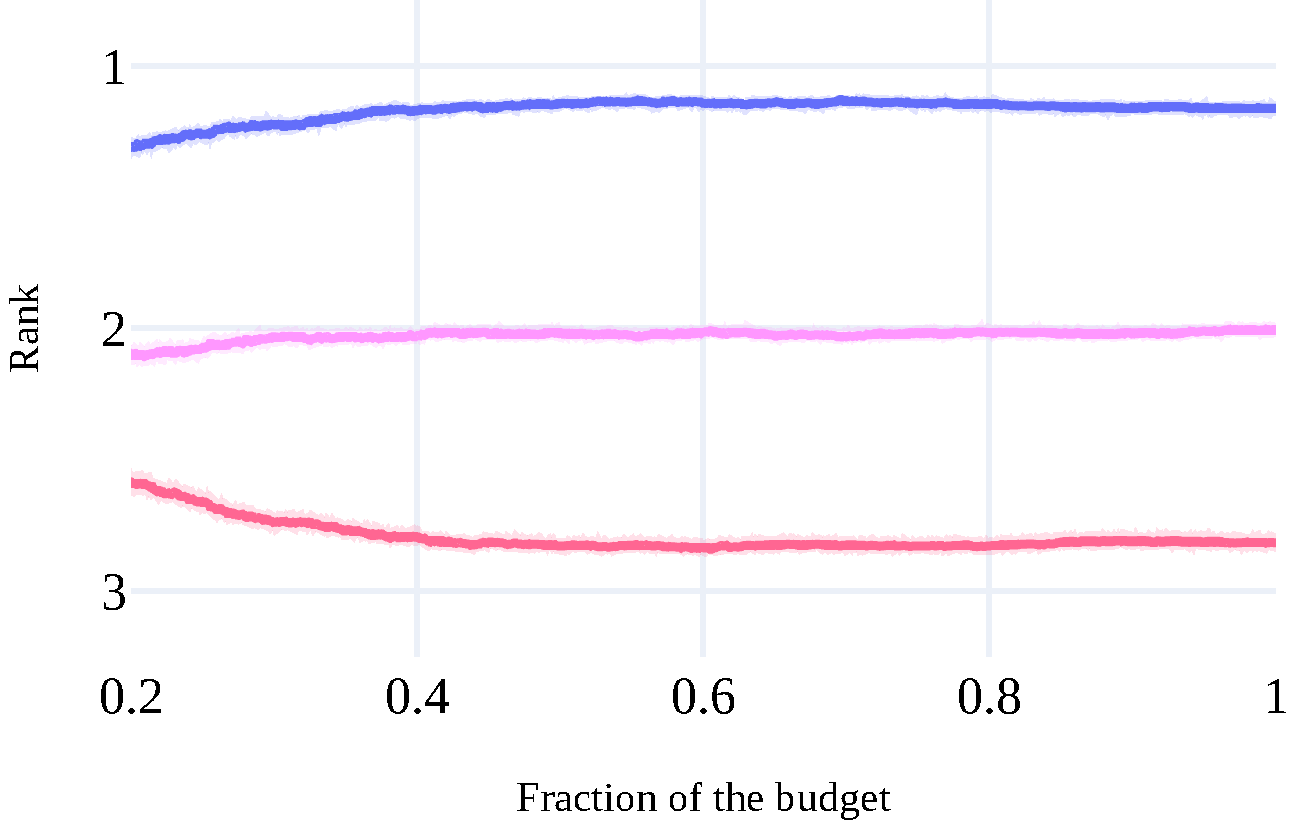
\includegraphics[scale=0.33]{figures/05/figs/figs/ranks/additional_baselines_all.pdf}
    \end{subfigure}
    
\includegraphics[scale=0.33]{figures/05/figs/figs/ranks/additional_baselines_all_legend.pdf}
    \caption{Comparison of \texttt{DyMBO} to simple selection and equal weights baselines as a function of the fraction of the wall-clock time budget on YAHPO Gym and JAHS-Bench-201. Our method outperforms both baselines.
    % \todo{missing line in te label}
    }
    \label{fig:ch05:add_baselines}

\end{figure*}


\paragraph{Selection of the best surrogate and equal weights.}
We compared our method to two additional baselines: one that simply averages the predictions of the surrogate models (RF and GP), and a simple selection baseline, which selects the best performing (\emph{i.e.}, most accurate) surrogate model after the initial 8 samples and uses only this model for the rest of the optimisation. 
Since both baselines are HEBO-based, they inherit MACE as the acquisition function.
We performed the selection using 8-fold cross-validation, and we used the MSE loss as an accuracy metric; we then chose the surrogate which yields the most accurate predictions. 
We provide the results in~\cref{fig:ch05:add_baselines}, where we see that our method outperforms both baselines. This emphasises the effectiveness of dynamically assigning weights to the surrogate models.

\paragraph{Random selection of surrogates.}
Finally, we compared our method to another simple selection baseline that chooses a surrogate uniformly at random in each iteration.
In this experiment, we used RF and GP as surrogate models with 8 initial samples.
% \changed{
\cref{fig:ch05:rnd_sel_rnk} shows that \texttt{DyMBO} maintains a substantially better mean rank throughout the optimisation. To further analyse this, we present in~\cref{fig:ch05:rnd_sel_ecdf} a task-level comparison of the final objective values, where we compare the log-scaled ratio between the final values \texttt{DyMBO} achieved and the final values that the random selection baseline achieved. Positive log-ratios show that \texttt{DyMBO} performs better, negative values show that random selection perform better, and zero indicates equal performance. \texttt{DyMBO} obtains a better final value on 406 of the 859 tasks, while random selection performs better on 262 tasks, and the two methods are tied on the remaining 191 tasks. These results indicate that the gains of \texttt{DyMBO} cannot be explained solely by randomly switching between complementary surrogate models, as selecting the surrogate according to its observed ranking accuracy provides a clear advantage over random switching.
% }


\begin{figure}
    \centering
    \begin{subfigure}[t]{0.49\textwidth}
        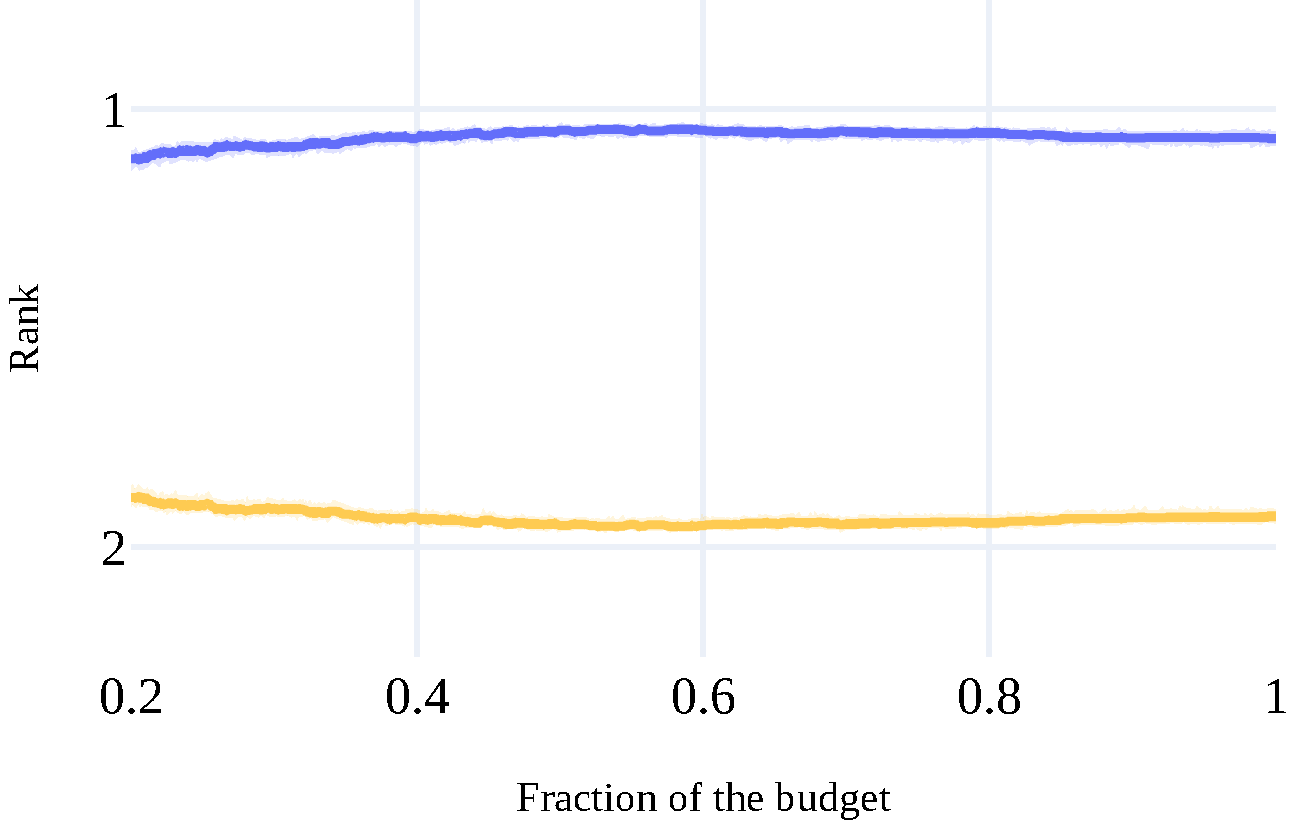
\includegraphics[scale=0.33]{figures/05/figs/figs/ranks/comp_rnd_choice2_all.pdf}
        \caption{}
        \label{fig:ch05:rnd_sel_rnk}
    \end{subfigure}
    
    \begin{subfigure}[t]{0.49\textwidth}
        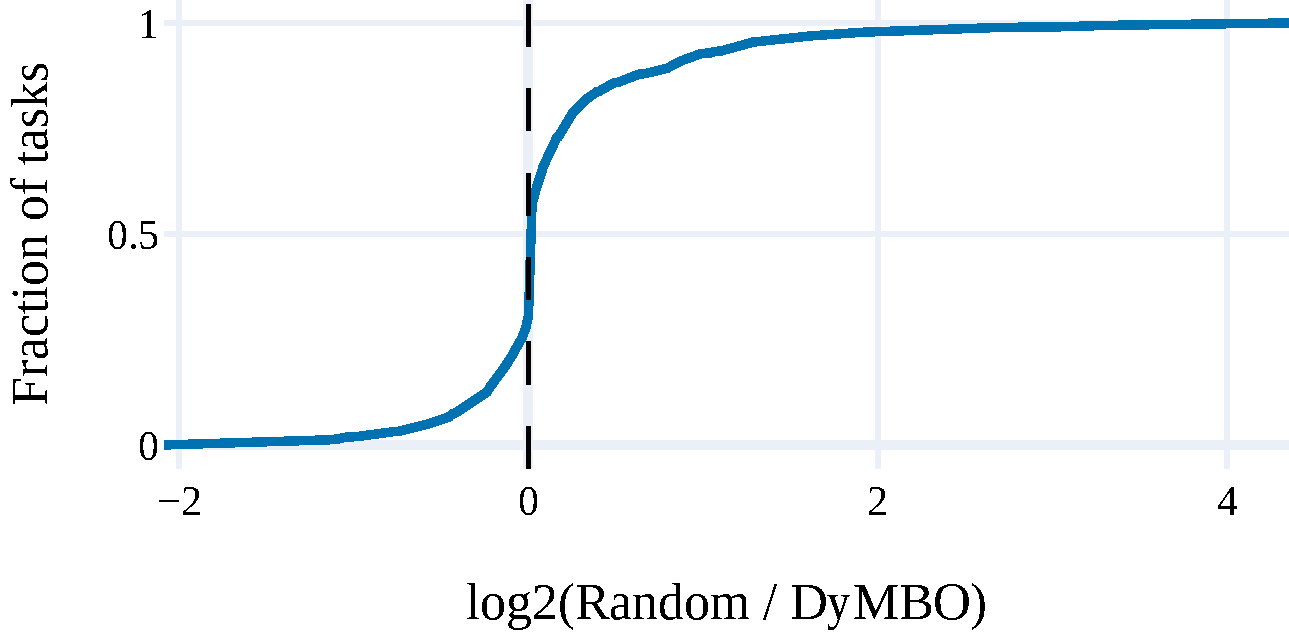
\includegraphics[scale=0.33]{figures/05/figs/figs/ranks/comp_rnd_choice_final_regret_log_ratio_ecdf.pdf}
        \caption{}
        \label{fig:ch05:rnd_sel_ecdf}
    \end{subfigure}
    
\includegraphics[scale=0.33]{figures/05/figs/figs/ranks/comp_rnd_choice2_all_legend.pdf}
    \caption{Comparison of \texttt{DyMBO} with $\alpha=1.0$ against a baseline that randomly selects between the RF and GP surrogates at every iteration, evaluated on YAHPO Gym and JAHS-Bench-201. (a) Mean rank as a function of the fraction of  wall-clock time budget for each task; lower ranks indicate better performance. (b) Empirical cumulative distribution (ECDF) across tasks of the log-ratio between the final objective values obtained by random selection and \texttt{DyMBO}. Positive values favour \texttt{DyMBO}, negative values favour random selection, and zero indicates equal performance. \texttt{DyMBO} performs better on 406 of the 859 tasks, random selection performs better on 262 tasks, and the remaining 191 tasks are tied.
    }
    \label{fig:ch05:random-surrogates}
\end{figure}


\section{Different setups of experiments}
\label{sec:ch05:diff_exp_setup}

We ran \texttt{DyMBO} with different setups of experiments in addition to the one corresponding to the main results from~\cref{sec:ch05:res_general}. We first explore the effects of using a fixed number of evaluations, as compared to a time-based budget. We then investigate the performance of our method with a varying size of initial design, \emph{i.e.}, for different numbers of initial random samples. 
We also look into whether different batch sizes affect the performance of \texttt{DyMBO}.

\paragraph{Fixed number of evaluations.}
\label{sec:ch05:256_evals}

In addition to the main results in~\cref{sec:ch05:res_general}, we performed additional experiments to assess the effectiveness of our method as a function of the number of evaluations and not as the budget measured in wall-clock time. 
We used 8 initial samples and a total budget of 512 evaluations. 
This additional experiment was designed to show the ability of the optimiser to find good-performing candidates, regardless of the running time required for the optimiser or the target function. 
We evaluated the approach on YAHPO Gym, and the results are presented in~\cref{fig:ch05:ranks512}.
We see that \texttt{DyMBO} outranks the single-surrogate baselines when budget is measured in terms of the number of function evaluations.
% Dynamic ensembling is ranked better, with $\alpha=0.9$ having the best performance, closely followed by $\alpha=1.0$. 
% All dynamic ensembling methods are ranked better than the single surrogate baselines, as well as the static ensemble with equal weights to all models.

\begin{figure}
    \centering
    % \begin{subfigure}[t]{0.49\textwidth}
        % \centering
    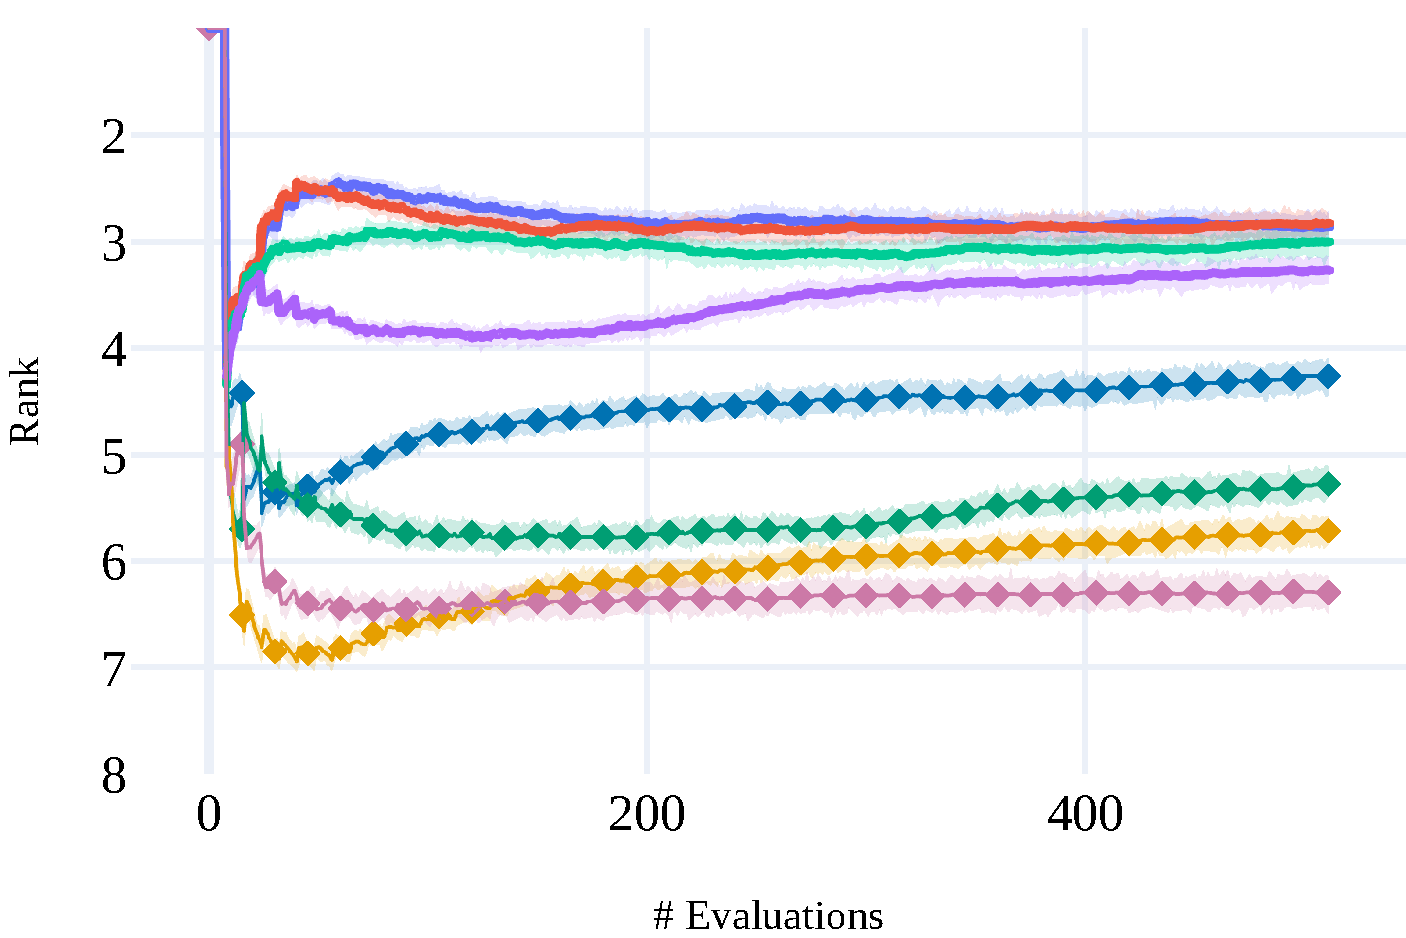
\includegraphics[scale=0.33]{figures/05/figs/figs/ranks/main_ranks_all_fixed.pdf}
    % \end{subfigure}
    % \begin{subfigure}[t]{0.49\textwidth}
    %     \centering
    %     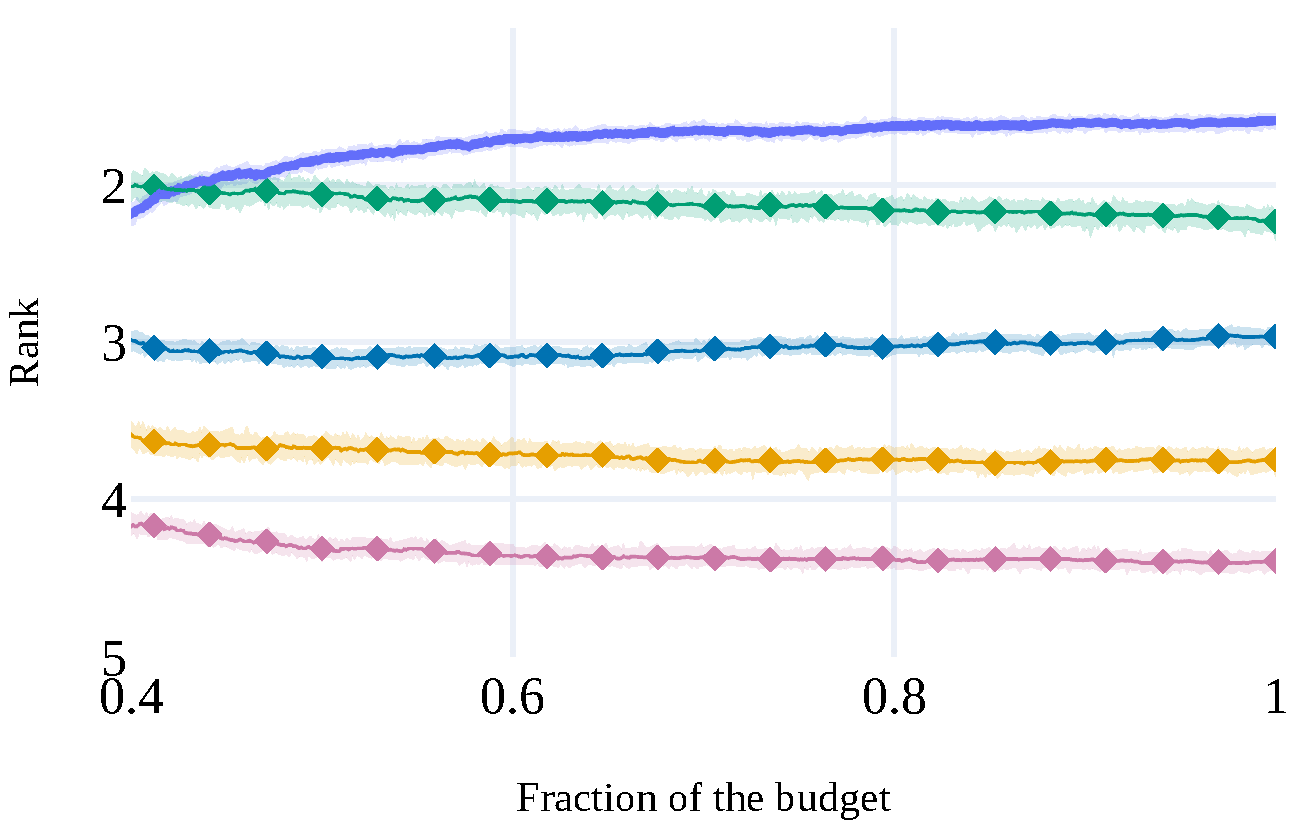
\includegraphics[scale=0.33]{figures/06/figs/figs/ranks/main_ranks_8_32_all.pdf}
    %     \caption{32}
    % \end{subfigure}
    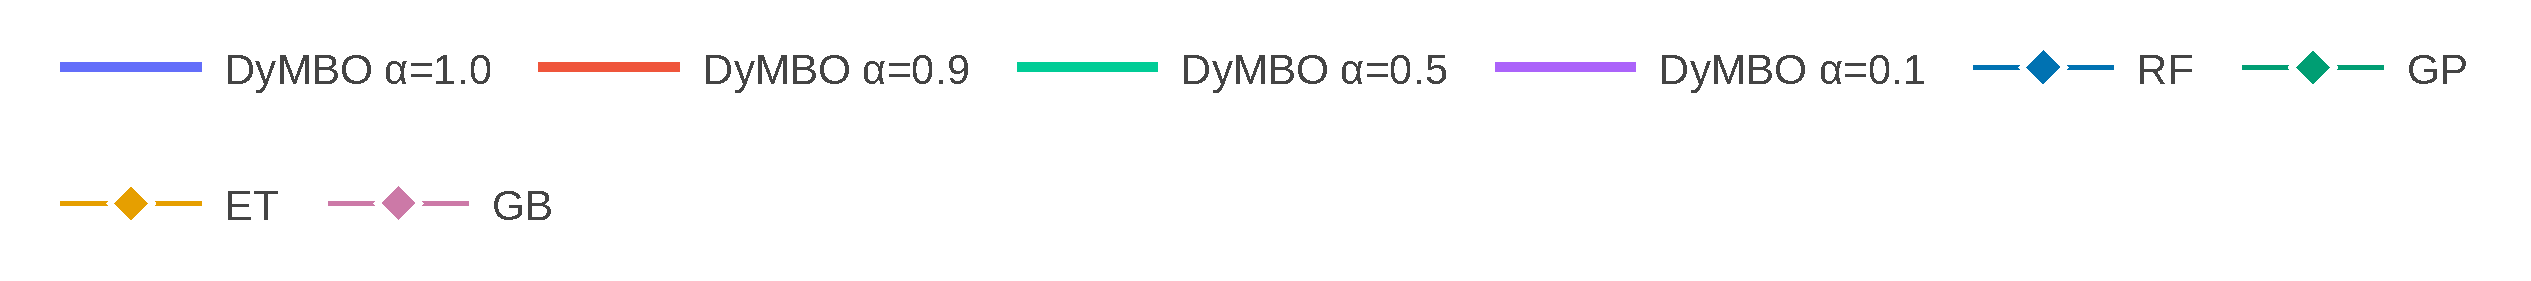
\includegraphics
    [scale=0.33]{figures/05/figs/figs/ranks/main_ranks_all_fixed_legend.pdf}
    \caption{Mean ranks of the different methods on YAHPO Gym and JAHS-Bench-201 as a function of the number of evaluations, with a total budget of 512 evaluations. \texttt{DyMBO} exhibits the best performance.
    }
    \label{fig:ch05:ranks512}
\end{figure}


\paragraph{Different number of initial samples.}
\label{sec:ch05:diff_init_samp}
We evaluated the performance of our method with different numbers of initial random samples. We used 16 and 32 initial samples, in addition to the 8 initial samples in~\cref{sec:ch05:res_general}. We used a total budget of $100\times$ average evaluation time. We evaluated the method on YAHPO Gym and JAHS-Bench-201, and the results are presented in~\cref{fig:ch05:diff_init_samp}. We see that \texttt{DyMBO} outperforms the single-surrogate baselines in all cases.

\begin{figure}
    \centering
    \begin{subfigure}[t]{0.49\textwidth}
        \centering
        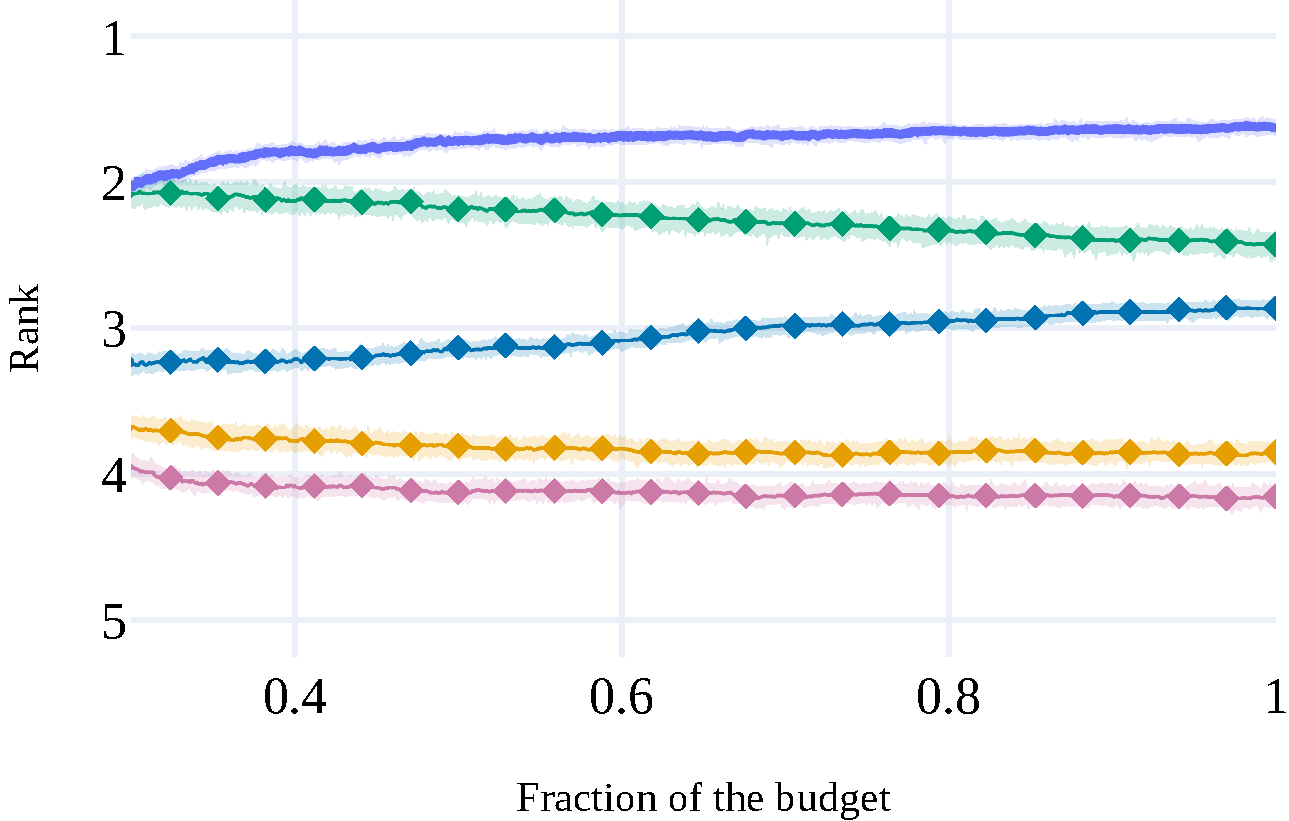
\includegraphics[scale=0.33]{figures/05/figs/figs/ranks/main_ranks_8_16_all.pdf}
        \caption{16 initial samples}
    \end{subfigure}
    \begin{subfigure}[t]{0.49\textwidth}
        \centering
        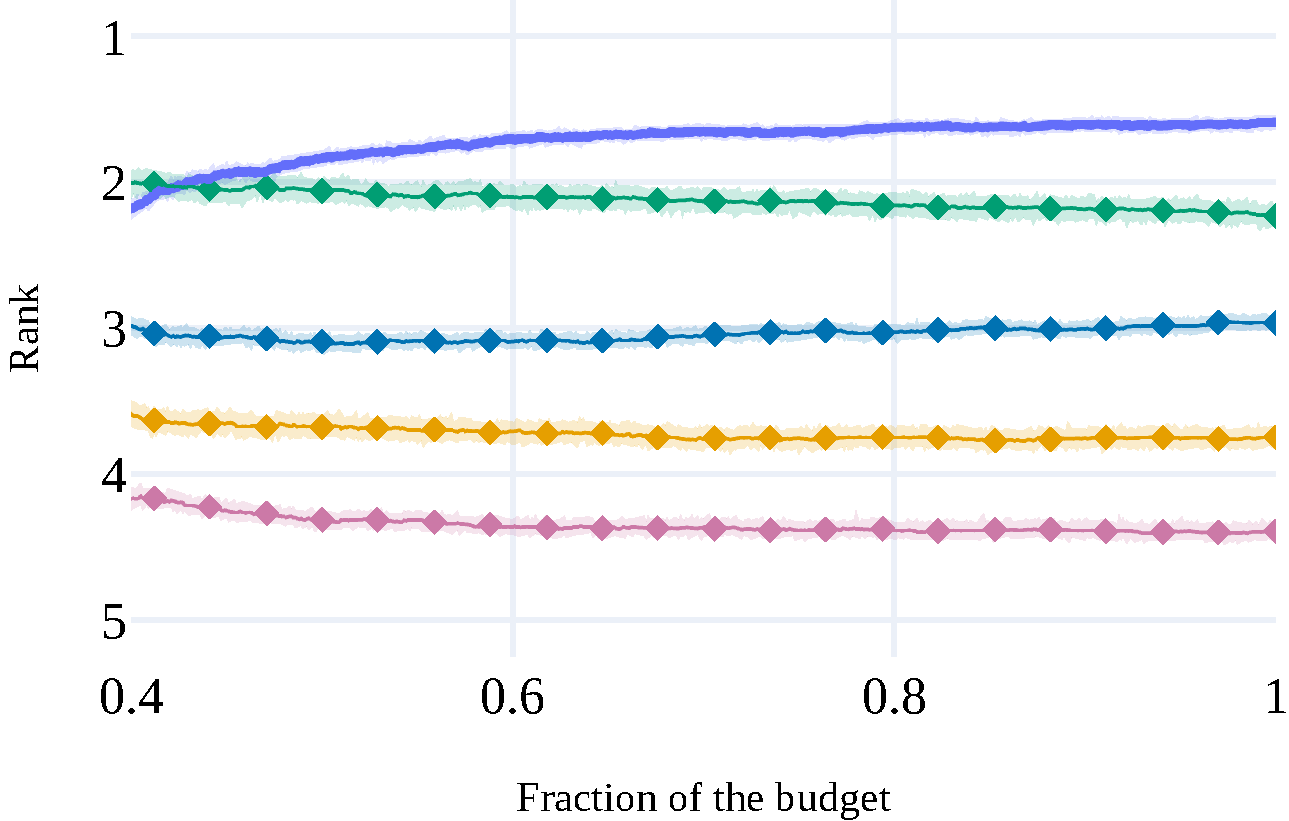
\includegraphics[scale=0.33]{figures/05/figs/figs/ranks/main_ranks_8_32_all.pdf}
        \caption{32 initial samples}
    \end{subfigure}
    \begin{subfigure}[t]{\textwidth}
        \centering
        
\includegraphics[scale=0.33]{figures/05/figs/figs/ranks/main_ranks_8_32_all_legend.pdf}
        % \caption{32 initial samples}
    \end{subfigure}
    
    \caption{Mean ranks with different numbers of initial samples as a function of the fraction of the wall-clock time budget on YAHPO Gym and JAHS-Bench-201. \texttt{DyMBO} achieves the best mean rank in both cases.
    % \todo{string "HEBO" can be dropped from the legends and explained in the caption, same for Fig.8 and Fig.9}
    }
    \label{fig:ch05:diff_init_samp}
\end{figure}

\paragraph{Different batch sizes.}
\label{sec:ch05:diff_batch_sizer}
We evaluated the performance of our method with different batch sizes. We used batch sizes of 1 (fully sequential sampling) and 4, in addition to the batch size of 8 in~\cref{sec:ch05:res_general}. For this experiment, we used a similar setup as in~\cref{sec:ch05:res_general}, with 8 initial samples and a total budget of $100\times$ average evaluation time. We evaluated the method on YAHPO Gym and JAHS-Bench-201, and the results are shown in~\cref{fig:ch05:diff_batch_sizer}. We see that with different batch sizes \texttt{DyMBO} also outperforms the single-surrogate baselines. We furthermore observe that RF performs better with batch sizes larger than 1, \emph{i.e.,} not in a fully sequential setup, based on both~\cref{fig:ch05:gen_res_simple,fig:ch05:diff_batch_sizer}.
% \aj{unresolved ref to fig}
% \er{Question: we say this only observing Figure 7, or also based on Figure 2, for batch size = 8?} \aj{We need to rephrase this a bit. For batch sizes 4 and 8 RF performs better than in a fully sequential setup. I don't see drastic differences in RF performance for batch 4 and batch 8.}

\begin{figure}
    \centering
    \begin{subfigure}[t]{0.49\textwidth}
        \centering
        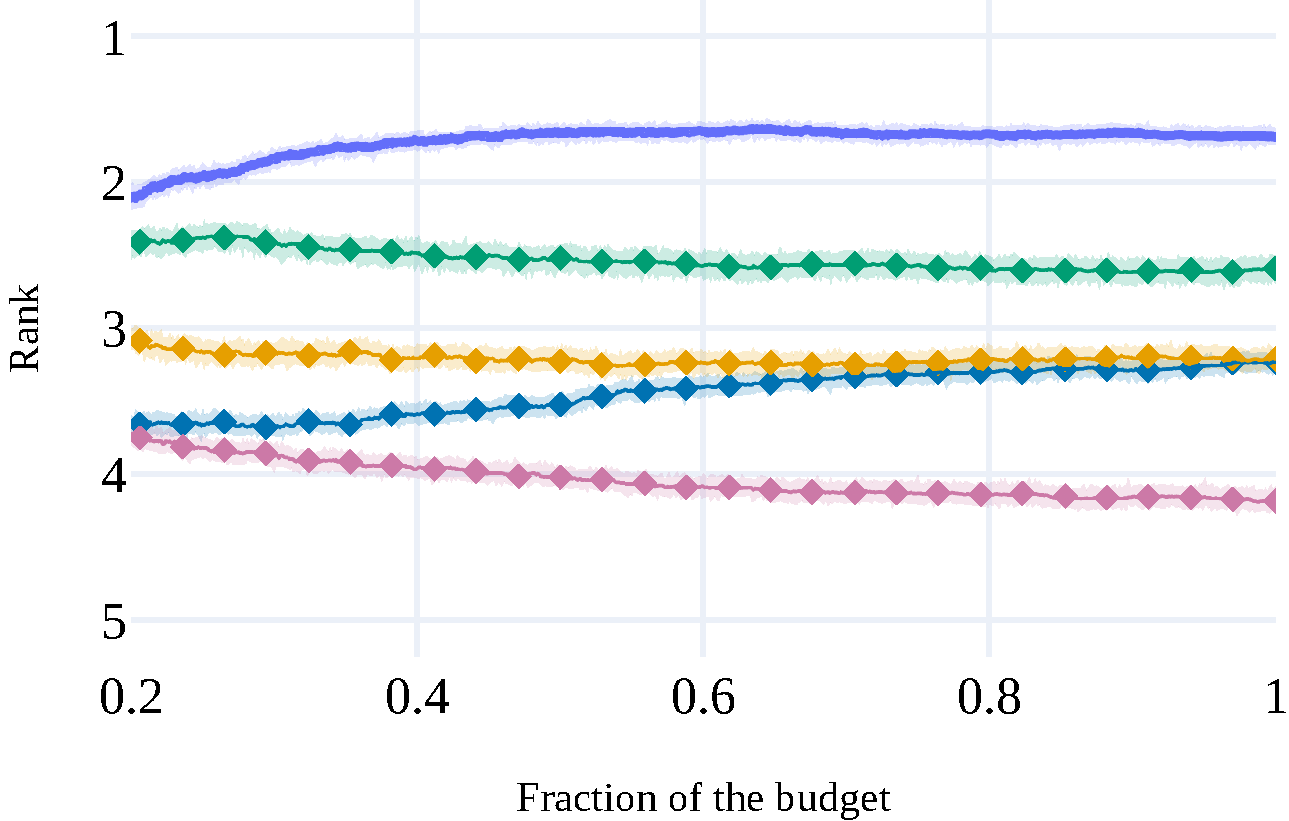
\includegraphics[width=\textwidth]{figures/05/figs/figs/ranks/main_ranks_1_8_all.pdf}
        \caption{Batch size 1 (fully sequential)}
    \end{subfigure}
    \begin{subfigure}[t]{0.49\textwidth}
        \centering
        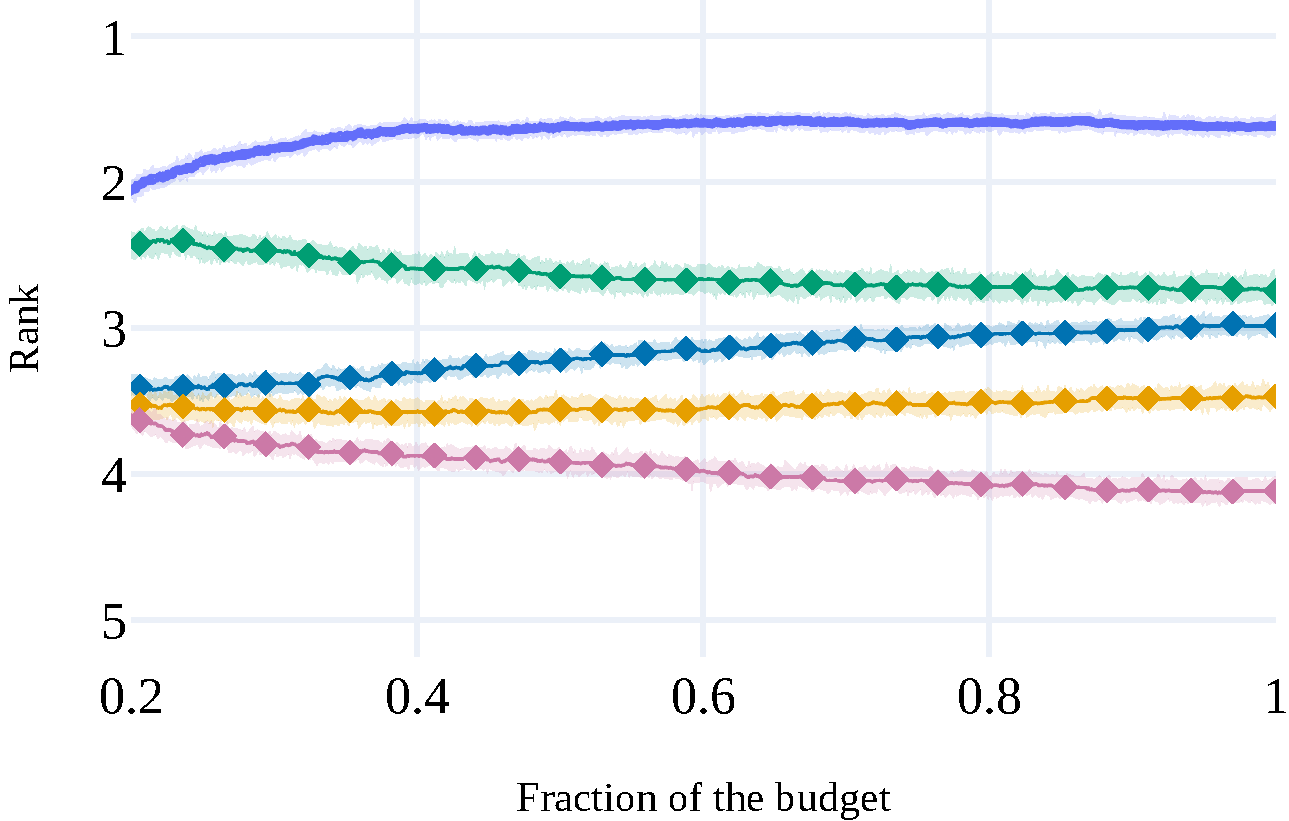
\includegraphics[width=\textwidth]{figures/05/figs/figs/ranks/main_ranks_4_8_all.pdf}
        \caption{Batch size 4}
    \end{subfigure}
    
\includegraphics[scale=0.33]{figures/05/figs/figs/ranks/main_ranks_4_8_all_legend.pdf}
    \caption{Mean ranks with different batch sizes as a function of the fraction of the wall-clock time budget on YAHPO Gym and JAHS-Bench-201. \texttt{DyMBO} has the best mean rank in both cases.
    % \todo{legend?}
    }
    \label{fig:ch05:diff_batch_sizer}
\end{figure}

\section{Ablation studies}
\label{sec:ch05:ablations}

% \er{Elena, readi this - new part (no H.3)} 
In this section, we describe several ablation studies we performed on our method. 
% In~\autoref{sec:app_alpha}, we first examine the effect of the value of the smoothing factor $\alpha$ of the exponential moving average for weight computation on the performance of \texttt{DyMBO}, \emph{i.e.}, how much the performance varies depending on the degree to which we rely on the history of model accuracies. \aj{remove}
We first investigate to what extent the choice of the acquisition function affects the performance of \texttt{DyMBO}. 
We also examine the effect of using independently computed weights for variance and of computing the total variance that accounts for both aleatoric and epistemic uncertainty.
We then assess the performance of \texttt{DyMBO} when using MSE as a more common metric for evaluating the model accuracy.
As we include four different surrogate models in our study, we also evaluate how \texttt{DyMBO} performs using ensembles constructed from all different combinations of these four surrogates.
Last, we explore different weight initialisation strategies, and look into how accuracy evaluation on a different number of observations impacts the performance of our method.


\paragraph{Changing the acquisition function.}
\label{sec:ch05:abl_af}
Our method is implemented in the HEBO framework, which by default uses the MACE acquisition function~\citep{LyuEtAl18}. 
Instead of deciding where to sample the next point based on a single criterion, MACE adopts a multi-objective perspective on this decision process by simultaneously optimising EI, PI and UCB as acquisitions.
This allows for a robust balance between exploration and exploitation, which are traded off in different ways using different acquisitions, by sampling the next point from the Pareto set resulting from this multi-objective optimisation.

% \todo{Could the MACE acquisition be explained more here, especially contrasting with acquisitions used in other baselines?}
In order to evaluate the effect of the acquisition function choice on our method, we experimented with the three stand-alone acquisition functions considered in MACE: EI, PI and UCB.
% \er{Can't we just use abbreviated names here? Or is too far from where we introduced the acronyms?} 
% \aj{we can, done.}
We ran \texttt{DyMBO} with EI, PI and UCB separately on YAHPO Gym and JAHS-Bench-201 with a budget of $100\times$ mean evaluation time per target function. We present the results in~\cref{fig:ch05:acqs}. We see that the MACE acquisition function performs better than the other three acquisition functions, especially with a larger budget, followed by EI and UCB.
\begin{figure}
    \centering
    % \begin{subfigure}[t]{0.49\textwidth}
        % \centering
        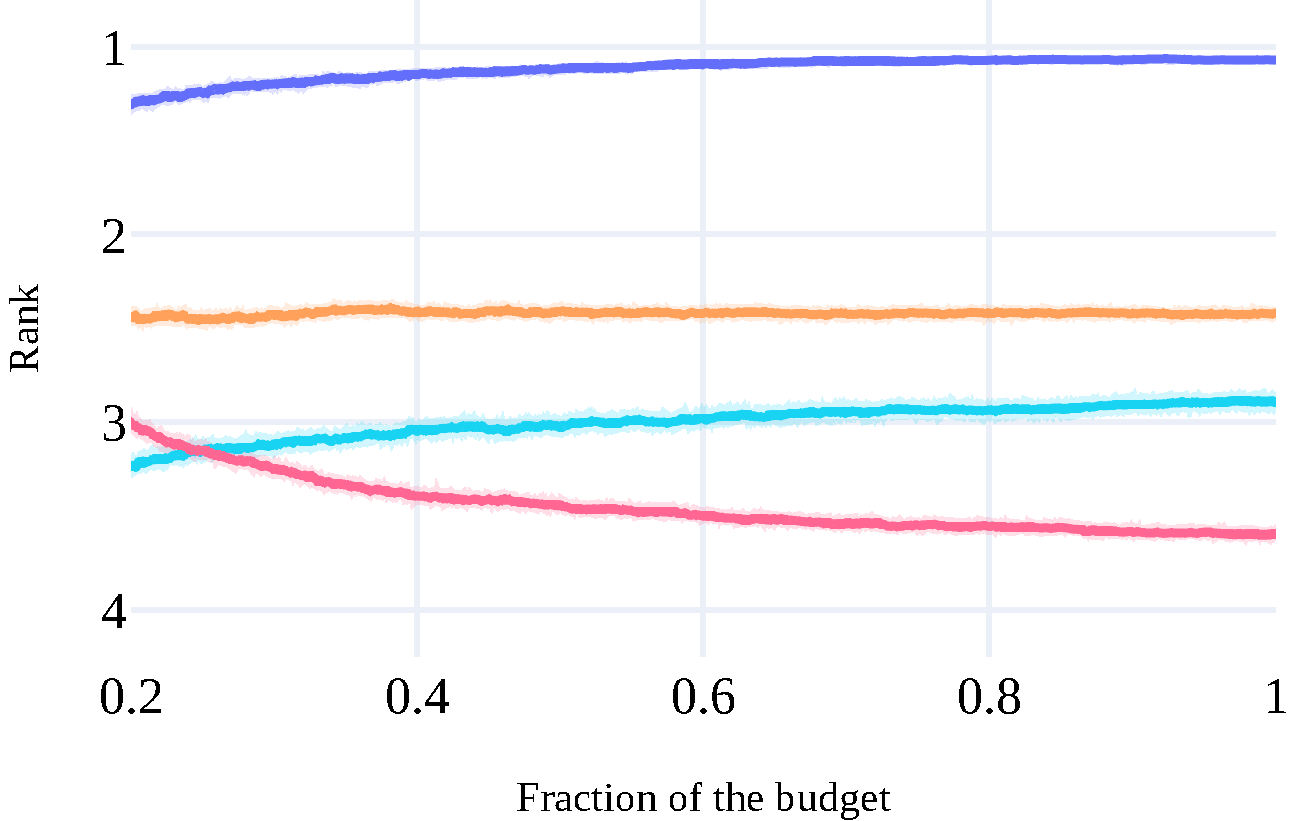
\includegraphics[scale=0.33]{figures/05/figs/figs/ranks/act_all.pdf}
        % \caption{32}
    % \end{subfigure}
    
\includegraphics[scale=0.33]{figures/05/figs/figs/ranks/act_all_legend.pdf}
    \caption{Mean ranks of \texttt{DyMBO} with different acquisition functions as a function of the fraction of the wall-clock time budget on YAHPO Gym and JAHS-Bench-201. Using MACE yields the best performance.}
    \label{fig:ch05:acqs}
\end{figure}

\paragraph{Using different weights for variance.}
\label{sec:ch05:with_variance}
We experimented with weighting the mean and the variance separately by having two, independent weight vectors. 
The weight vector of the mean is the same as described in~\cref{sec:ch05:method}. 
For the variance weights,
% \changed{
we introduce variance error (VE) as a non-probabilistic measure of calibration that does not require additional assumptions about the underlying predictive distribution. In contrast, metrics such as log-likelihood evaluate the full predictive distribution and therefore require a well-specified noise model, which is less straightforward for some surrogates, such as tree-based models.
% }

We define VE for a model $m\in M$ as follows:
% \todo{Could any references for the variance error be included?}
\begin{equation}
    \text{VE}_m(\lambda_t) = \frac{1}{k}\sum_{i=1}^{k} \min \{|(\mu_m(\lambda_t^{(i)}) - \sigma_m(\lambda_t^{(i)}))- c(\lambda_t^{(i)})|,  |(\mu_m(\lambda_t^{(i)}) + \sigma_m(\lambda_t^{(i)}))- c(\lambda_t^{(i)})|\}
\end{equation}
Intuitively, it is the distance to the closest variance bound, as can be seen in~\cref{fig:ch05:gen_res_var}. 
Since computing $\text{VE}_m(\lambda_t)$ relies on the true function value $c(\lambda_t)$, this error can only be calculated post-hoc on points that have already been fully evaluated.
We update the weights for variance accordingly. 
The new weights are defined as:
\begin{equation}\label{eqn:ch05:weight_var}
    {w}'_{t,m}=
    \begin{cases}
        1 & \text{if } \text{VE}_m(\lambda_t)=\text{min}_{l\in M} \text{VE}_l(\lambda_t),  \\
        0 & \text{otherwise},
    \end{cases}
\end{equation}
We calculate the weights for variances using the exponential moving average:
\begin{equation}
    \bar{w}'_{t+1,m} = (1-\alpha) \cdot \bar{w}'_{t, m} + \alpha  \cdot {w}'_{t,m} \; ,
    \label{eq:ch05:weight_ema_var}
\end{equation}
Then, we normalise the weights for the variances independently from the weights for the means:
\begin{equation}
    \hat{w}'_{t,m} = \frac{\bar{w}'_{t,m}}{\sum_{j\in M}{\bar{w}'_{t, j}}},
\end{equation}
Finally, the variance predicted by the ensemble is defined as the weighted sum of the normalised weights of the variances:
\begin{equation}
    \sigma_{\text{ens}}(\lambda)= \sum_{m\in M} \hat{w}'_{t,m} \cdot \sigma_{m}(\lambda).
    \label{eq:ch05:ens_sigma_var}
\end{equation}
% \changed{
We note that VE is a custom metric introduced in this work to measure the accuracy of the predicted uncertainty bounds, analogous to the interval score used in proper scoring rules~\citep{GneRaf07}.
% }

We ran \texttt{DyMBO} with variance with $\alpha=0.9$ and a budget of $100\times$ mean evaluation time per target function. 
Similarly to the results presented in~\cref{sec:ch05:res_general}, we present the mean rank of all methods, including \texttt{DyMBO} with different weights for variances in~\cref{fig:ch05:gen_res_var}. 
The experimental setup is similar to~\cref{sec:ch05:res_general}, where the budget is $100\times$ mean running time of one evaluation. 
We see in~\cref{fig:ch05:diff_var_w} that using different weights for variance ranks worse than \texttt{DyMBO} with the same weights for both the means and variances.
\begin{figure*}
    \centering
    \begin{subfigure}[t]{0.49\textwidth}
        \centering
        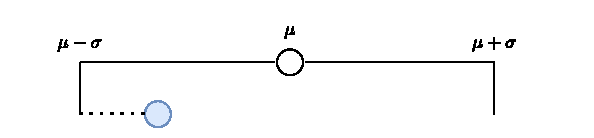
\includegraphics[width=\textwidth]{figures/05/figs/variance/ens_var_error_1.pdf}
        \caption{}
    \end{subfigure}
    \begin{subfigure}[t]{0.49\textwidth}
        \centering
        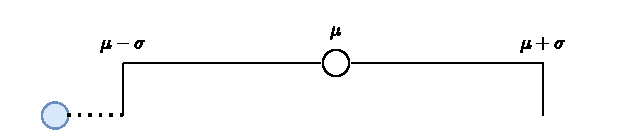
\includegraphics[width=\textwidth]{figures/05/figs/variance/ens_var_error_2.pdf}
        \caption{}
    \end{subfigure}
    \begin{subfigure}[t]{0.49\textwidth}
        \centering
        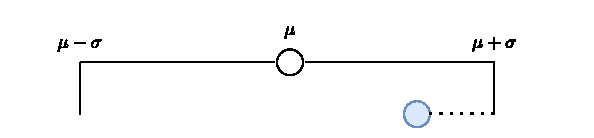
\includegraphics[width=\textwidth]{figures/05/figs/variance/ens_var_error_3.pdf}
        \caption{}
    \end{subfigure}
    \begin{subfigure}[t]{0.49\textwidth}
        \centering
        \includegraphics[width=\textwidth]{figures/05/figs/variance/ens_var_error_4.pdf}
        \caption{)}
    \end{subfigure}
    \caption{Illustration of the calculation of the variance error. The white dot is the predicted mean, and the blue dot is the actual value of the target function.
    We distinguish between four cases, depending on whether the actual value of the target function lies within or outside of the uncertainty bounds around the predicted mean, and whether it is smaller or larger than the value of the predicted mean.
    % \todo{Making this a representative example of how the argmin is being used will utilize this plot better.}
    % \aj{I have no idea what this comment means...}
    }
    \label{fig:ch05:gen_res_var}
\end{figure*}

\begin{figure}
    \centering
    % \begin{subfigure}[t]{0.49\textwidth}
    \includegraphics[scale=0.33]{figures/05/figs/figs/ranks/diff_var_w_all.pdf}
    \includegraphics[scale=0.33]{figures/05/figs/figs/ranks/diff_var_w_all_legend.pdf}
    \caption{Comparison of \texttt{DyMBO} with same weights for means and variances and \texttt{DyMBO} with different weights for means and variances as a function of the fraction of the wall-clock time budget on YAHPO Gym and JAHS-Bench-201. Same weights for means and variances yield better performance.}
    \label{fig:ch05:diff_var_w}
\end{figure}



\paragraph{Using the rule of total variance.}
\label{sec:ch05:abl_totalvar}
We considered computing the variance of the ensemble using the rule of total variance. Such calculation was proposed by~\citet{HutEtAl14} and~\citet{KenGal17}, where the total variance was decomposed into aleatoric uncertainty (noise inherent to the data) and epistemic uncertainty (disagreement between models). We calculate the total variance of the ensemble as follows:
\begin{equation}
    \sigma^2 = \sum_{m\in M} \hat{w}_m \sigma_m^2 + \sum_{m\in M} \hat{w}_m \mu_m^2 - \left(\sum_{m\in M} \hat{w}_m \mu_m\right)^2
\end{equation}

By using the rule of total variance, we add the measure of the correlation between the means and the variances of the models (\emph{i.e.}, epistemic uncertainty) to our initial variance equation that captures aleatoric uncertainty. We ran \texttt{DyMBO} with total variance with $\alpha=0.9$ and a budget of $100\times$ mean evaluation time per target function. We present the results in~\cref{fig:ch05:total_variance}. We see that using total variance ranks worse than \texttt{DyMBO} with aleatoric-only variance.
\begin{figure}
    \centering
    \begin{subfigure}[t]{0.49\textwidth}
    \centering
    \includegraphics[scale=0.33]{figures/05/figs/figs/ranks/total_variance_all.pdf}
    \end{subfigure}
    \begin{subfigure}[t]{1\textwidth}
        \centering
    \includegraphics[scale=0.33]{figures/05/figs/figs/ranks/total_variance_all_legend.pdf}
    \end{subfigure}

    \caption{Comparison of \texttt{DyMBO} which computes the variance using the rule of total variance to \texttt{DyMBO} which computes the variance as a weighted sum of the variances as a function of the fraction of the wall-clock time budget on YAHPO Gym and JAHS-Bench-201. Weighted sum of variances yields better performance.}
    \label{fig:ch05:total_variance}
\end{figure}

\paragraph{Considering different loss functions.}
\label{sec:ch05:loss_ablation}
In \texttt{DyMBO}, we use ranking loss as the loss function, as we are interested in identifying where the optimum lies, as opposed to having a model with the most accurate actual predictions. %Indeed, by preserving the pairwise ordering of predicted function values which is to decide which configurations to evaluate next, \emph{i.e.}, to identify promising regions of the search space. 
% The optimisation trajectory relying on the model would therefore still be driven towards promising regions, without using model capacity to perfectly fit the data, which is particularly important when we have limited evaluation budget.
% On the other hand, 
The predictive power of a model is better reflected by more common loss functions for regression tasks, such as mean squared error (MSE). We thus evaluated the performance of \texttt{DyMBO} when using MSE as a metric for model accuracy: 
% \todo{add parameters}\hh{still to be done?}
\begin{equation}
    \text{MSE}(\mu_m, \boldsymbol{\lambda}) = \frac{1}{n} \cdot\sum_{\lambda^{(j)}\in \boldsymbol{\lambda}} (\mu_m(\lambda^{(j)}) - c(\lambda^{(j)}))^2.
\end{equation}
We ran \texttt{DyMBO} with MSE as a loss function on YAHPO Gym and JAHS-Bench-201 with a budget of $100\times$ mean evaluation time per target function. We present the results in~\cref{fig:ch05:loss_ablation}. We see that \texttt{DyMBO} using ranking loss performs slightly better than \texttt{DyMBO} using MSE.
\begin{figure}
    \centering
    \includegraphics[scale=0.33]{figures/05/figs/figs/ranks/loss_all.pdf}
    \includegraphics[scale=0.33]{figures/05/figs/figs/ranks/loss_all_legend.pdf}

    \caption{Mean ranks of \texttt{DyMBO} with different loss functions (ranking loss vs. MSE) as a function of the fraction of the wall-clock time budget on YAHPO Gym and JAHS-Bench-201. Ranking loss performs better than MSE, especially in low budgets.}
    \label{fig:ch05:loss_ablation}
\end{figure}

\paragraph{Varying the combinations of surrogate models in the ensemble.}
\label{sec:ch05:models_choice}
We evaluated the performance of \texttt{DyMBO} with different surrogate models as part of the ensemble. Having more surrogate models allows for better best-found configurations 
% \aj{what do we mean by maximal results?}\er{best-found results?}\aj{I would replace it with "best-found solutions" or "configurations", pls check how it reads} 
as the ensemble can choose the best model for each target function. However, including more models also increases the risk of choosing a model that performs poorly. We ran \texttt{DyMBO} with different combinations of 4 surrogate models: RF, GP, GB, and ET. We used a budget of $100\times$ mean evaluation time per target function. We present the results in~\cref{fig:ch05:models_choice}. We observe best performance by using only RF and GP, followed by using RF, GP and ET.
\begin{figure}
    \centering
    \includegraphics[scale=0.33]{figures/05/figs/figs/ranks/models_choice_all.pdf}
    \includegraphics[scale=0.33]{figures/05/figs/figs/ranks/models_choice_all_legend.pdf}
    \caption{Mean ranks of \texttt{DyMBO} with different surrogate models as a function of the fraction of the wall-clock time budget on YAHPO Gym and JAHS-Bench-201. Using the combination of RF and GP yields the best performance.}
    \label{fig:ch05:models_choice}
\end{figure}

\paragraph{Using different weight initialisation strategies.}
\label{sec:ch05:init_ablation}
We experimented with different weight initialisation schemes to assess how they affect the performance of \texttt{DyMBO}. In addition to initialising with RF (with $w_{RF}=1$ and $w_{GP}=0$ as in~\cref{sec:ch05:experiments}), we also considered initialising with GP: $w_{GP}=1$ and $w_{RF}=0$. Additionally, we tested initialising with both models: $w_{RF}=1$ and $w_{GP}=1$. Finally, we tried a heuristic initialisation, where we set $w_{RF}=1$ if the target function has categorical hyperparameters, and $w_{GP}=1$ if the target function is cheap. The rest of the weights are set to 0. 
% \er{Just a comment about aesthetics... many times in the manuscript, the last line of a paragraph is composed of 1 word only. Am I allowed to slightly shorten so that this does not happen? Maybe we can also gain some space given the page limit.} \aj{I agree and also don't like a short last sentence. If you have an idea on how to shorten so that the meaning stays the same, please go ahead :)}

We ran \texttt{DyMBO} with different weight initialisation schemes on YAHPO Gym and JAHS-Bench-201 with a budget of $100\times$ mean evaluation time per target function. We show the results in~\cref{fig:ch05:init-ablation}. We see similar ranks between the different initialisation schemes, with the best performance achieved by initialising with RF.

\begin{figure}
    \centering
    \includegraphics[scale=0.33]{figures/05/figs/figs/ranks/init_ablation_all.pdf}
    \includegraphics[scale=0.33]{figures/05/figs/figs/ranks/init_ablation_all_legend.pdf}
    \caption{Mean ranks of \texttt{DyMBO} with different initialisation schemes as a function of the fraction of the wall-clock time budget on YAHPO Gym and JAHS-Bench-201.  Initialising with RF yields the best performance, although the differences are small.}
    \label{fig:ch05:init-ablation}
\end{figure}

\paragraph{Varying the number of points for accuracy evaluation.}
\label{sec:ch05:abl_eval_all}

We tested whether evaluating the model accuracy on all previously sampled points (\emph{i.e.}, the full history of observations) yields better performance than evaluating only on the last batch of points (\emph{i.e.}, observations from the last iteration only, which corresponds to having a train-test split). In the latter setting, computation of the new weights for the models was adapted accordingly so as to depend only on the accuracy from the last iteration. We ran \texttt{DyMBO} in this setting with a budget of $100\times$ mean evaluation time per target function. We show the results in~\cref{fig:ch05:eval-all}. We see that evaluating on the entire history of observations yields better performance than evaluating only on the last batch of points.
\begin{figure}
    \centering
    \centering
    \includegraphics[scale=0.33]{figures/05/figs/figs/ranks/eval_all_all.pdf}
    \includegraphics[scale=0.33]{figures/05/figs/figs/ranks/eval_all_all_legend.pdf}
    \caption{Comparison of original \texttt{DyMBO} (which evaluates on all points) to \texttt{DyMBO} which evaluates only on the last batch of points as a function of the fraction of the wall-clock time budget on YAHPO Gym and JAHS-Bench-201.
    % \todo{legend}
    }
    \label{fig:ch05:eval-all}
\end{figure}

\section{Results per search space}
\label{sec:ch05:res-search-space}

We analysed the performance of our method based on search space characteristics, offering insights into the efficacy of dynamic ensembling and selection of different surrogates that excel in various types of search spaces.
We provide the results for mixed discrete-continuous and numerical search spaces in~\cref{fig:ch05:search-spaces1,fig:ch05:search-spaces2}.
We see that all \texttt{DyMBO} variants are consistently top-ranked regardless of the nature of the search space, with exception of the rbv2\_svm scenario in~\cref{fig:ch05:rbv2_svm}, based on optimising hyperparameters of a support vector machine (SVM), for which Optuna AutoSampler exhibits the best performance.
% \todo{check if true, legend}

For certain mixed discrete-continuous search spaces, \emph{e.g.,} scenarios in~\cref{fig:ch05:rbv2_aknn,fig:ch05:rbv2_ranger,fig:ch05:rbv2_rpart}, \texttt{DyMBO} variants with $\alpha = 0.9$ and $\alpha = 1.0$ perform notably well, with low variance in performance, emphasising the advantage of either a strong reliance on the newly assigned weights or a pure selection in those cases.
For other mixed discrete-continuous spaces, \emph{e.g.,} scenarios in~\cref{fig:ch05:rbv2_glmnet,fig:ch05:rbv2_super,fig:ch05:rbv2_xgboost}, \texttt{DyMBO} variants with medium or very low values of $\alpha$ are top performers, revealing that our method can leverage not only the complementary strengths of different surrogates, but that having a possibility to rely more strongly on the history of surrogate accuracies can be crucial for the overall performance of the method.
For numerical-only search space in~\cref{fig:ch05:lcbench}, all \texttt{DyMBO} variants outperform single surrogates and other HPO methods, with a notable gap in ranks between \texttt{DyMBO} and the next-best method.

\begin{figure*}
    \centering
    \begin{subfigure}[t]{0.49\textwidth}
        \centering
        \includegraphics[scale=0.33]{figures/05/figs/figs/ranks/main_ranks_rbv2_aknn.pdf}
        \caption{rbv2\_aknn: $6D$ mixed discrete-continuous search space}
        \label{fig:ch05:rbv2_aknn}
    \end{subfigure}
    \begin{subfigure}[t]{0.49\textwidth}
        \centering
        \includegraphics[scale=0.33]{figures/05/figs/figs/ranks/main_ranks_rbv2_glmnet.pdf}
        \caption{rbv2\_glmnet: $3D$ mixed discrete-continuous search space}
        \label{fig:ch05:rbv2_glmnet}
    \end{subfigure}
        \begin{subfigure}[t]{0.49\textwidth}
        \centering
        \includegraphics[scale=0.33]{figures/05/figs/figs/ranks/main_ranks_rbv2_ranger.pdf}
        \caption{rbv2\_ranger: $8D$ mixed discrete-continuous search space}
        \label{fig:ch05:rbv2_ranger}
    \end{subfigure}
        \begin{subfigure}[t]{0.49\textwidth}
        \centering
        \includegraphics[scale=0.33]{figures/05/figs/figs/ranks/main_ranks_rbv2_rpart.pdf}
        \caption{rbv2\_rpart: $5D$ mixed discrete-continuous search space}
        \label{fig:ch05:rbv2_rpart}
    \end{subfigure}
    \includegraphics[scale=0.33]{figures/05/figs/figs/ranks/main_ranks_rbv2_xgboost_legend.pdf}
    \caption{Mean ranks of \texttt{DyMBO} (with different values of $\alpha$), HEBO with different surrogate models, and other HPO methods, as a function of the fraction of the wall-clock time budget on benchmarks from YAHPO Gym, split by search space characteristics (mixed discrete-continuous or numerical only). Variants of \texttt{DyMBO} are consistently top-ranked across different types of search spaces and different dimensionalities.
    }
    \label{fig:ch05:search-spaces1}
\end{figure*}

\begin{figure*}
    \centering
    \begin{subfigure}[t]{0.49\textwidth}
        \centering
        \includegraphics[scale=0.33]{figures/05/figs/figs/ranks/main_ranks_rbv2_super.pdf}
        \caption{rbv2\_super: $38D$ mixed discrete-continuous search space}
        \label{fig:ch05:rbv2_super}
    \end{subfigure}
    \begin{subfigure}[t]{0.49\textwidth}
        \centering
        \includegraphics[scale=0.33]{figures/05/figs/figs/ranks/main_ranks_rbv2_svm.pdf}
        \caption{rbv2\_svm: $6D$ mixed discrete-continuous search space}
        \label{fig:ch05:rbv2_svm}
    \end{subfigure}
    \begin{subfigure}[t]{0.49\textwidth}
        \centering
        \includegraphics[scale=0.33]{figures/05/figs/figs/ranks/main_ranks_rbv2_xgboost.pdf}
        \caption{rbv2\_xgboost: $14D$ mixed discrete-continuous search space}
        \label{fig:ch05:rbv2_xgboost}
    \end{subfigure}
    \begin{subfigure}[t]{0.49\textwidth}
        \centering
        \includegraphics[scale=0.33]{figures/05/figs/figs/ranks/main_ranks_lcbench.pdf}
        \caption{lcbench: $7D$ numerical search space}
        \label{fig:ch05:lcbench}
    \end{subfigure}
    \includegraphics[scale=0.33]{figures/05/figs/figs/ranks/main_ranks_rbv2_xgboost_legend.pdf}
    \caption{Mean ranks of \texttt{DyMBO} (with different values of $\alpha$), HEBO with different surrogate models, and other HPO methods, as a function of the fraction of the wall-clock time budget on benchmarks from YAHPO Gym, split by search space characteristics (mixed discrete-continuous or numerical only). Variants of \texttt{DyMBO} are consistently top-ranked across different types of search spaces and different dimensionalities.
    }
    \label{fig:ch05:search-spaces2}
\end{figure*}

\section{Benchmark details}
\label{sec:ch05:benchs}

\textbf{Yet Another HPO Benchmark (YAHPO) Gym}~\citep{PfiEtAl22} is a surrogate-based benchmark for hyperparameter optimisation on tabular machine learning tasks. 
The benchmark consists of multiple datasets from OpenML and various machine learning algorithms. 
The authors provide a surrogate model for each machine learning algorithm and a dataset that predicts different objectives, such as accuracy, training time, and more.

YAHPO Gym contains several scenarios. 
Each scenario has a configuration space and is based on a machine learning algorithm. 
Each scenario contains multiple datasets, which are called instances. 
The YAHPO Gym scenarios are: \\
% \begin{itemize}
    \textbf{rbv2\_ranger}~\citep{BinEtAl20}: RF using the ranger R implementation.\\ 
    \textbf{rbv2\_rpart}~\citep{BinEtAl20}: decision tree using the mlr implementation.\\
    \textbf{rbv2\_glmnet}~\citep{BinEtAl20}: generalised linear models (GLM) with elastic net regularisation using the mlr implementation.\\
    \textbf{rbv2\_svm}~\citep{BinEtAl20}: support vector machine (SVM) with the mlr implementation.\\
    \textbf{rbv2\_xgboost}~\citep{BinEtAl20}: gradient boosting using XGBoost.\\
    \textbf{rbv2\_aknn}~\citep{BinEtAl20}: k-nearest neighbours using the mlr implementation.\\
    \textbf{rbv2\_super}~\citep{BinEtAl20}: a combined algorithm selection and hyperparameter optimisation (CASH) scenario that uses all the above rbv2 scenarios.\\
    \textbf{iaml\_glment}~\citep{PfiEtAl22}: generalised linear models (GLM) with elastic net regularisation using the mlr implementation.\\
    \textbf{iaml\_rpart}~\citep{PfiEtAl22}: decision tree using the mlr implementation.\\
    \textbf{iaml\_ranger}~\citep{PfiEtAl22}: RF using the ranger R implementation.\\
    \textbf{iaml\_xgboost}~\citep{PfiEtAl22}: gradient boosting using XGBoost.\\
    \textbf{iaml\_super}~\citep{PfiEtAl22}: combined algorithm selection and hyperparameter optimisation (CASH) scenario that uses all the above iaml scenarios.\\
    \textbf{LCBench}~\citep{ZimEtAl21}: optimising the training hyperparameters and architecture of multi-layer perceptron on tabular datasets.\\
    \textbf{FCNet}~\citep{FalEtAl18}: hyperparameter optimisation of a fully-connected network for tabular data.\\
    \textbf{NAS-Bench-301}~\citep{ZelEtAl22}: neural architecture search (NAS) scenario using a constant set of training hyperparameters. The search space describes a cell of the neural network and the hyperparameters are different operations done in each cell.
% \end{itemize}

For details on configuration spaces, we refer the reader to original papers.
The configuration spaces for the rbv2 scenarios are taken from~\citep{BinEtAl20}. 
For rbv2\_super, the configuration space contains all the configuration spaces of individual algorithms, with an additional hyperparameter which selects the algorithm. 
The configuration spaces for the iaml scenarios are taken from~\citep{PfiEtAl22}; the iaml\_super scenario is similar to rbv2\_super, where there is an additional hyperparameter to select the algorithm. 
While the iaml and rbv2 scenarios look similar, there are a few differences in the configuration space. 
First, the configuration space of rbv2 contains the input imputation used, while in iaml the input imputation is constant. 
Another difference is a different range of hyperparameters (for example, the number of rounds in XGBoost). 
In all scenarios, the target metric is accuracy, as defined in~\citep{PfiEtAl22}.  
The configuration spaces for LCBench, FCNet and NAS-Bench-301 are taken from~\citep{ZimEtAl21,FalEtAl18,ZelEtAl22}, respectively.
Additionally, we benchmarked our method on \textbf{JAHS-Bench-201}~\citep{BanEtAl22}: a neural architecture search (NAS) benchmark that optimises both the architecture of the neural network and the training hyperparameters. The benchmark contains three datasets: CIFAR10, Fashion MNIST and Colorectal Histology.

\paragraph{Evaluation budget.}
All YAHPO Gym and JAHS-Bench-201 surrogates predict the running time required to train and evaluate the model using a specific configuration. 
Therefore, we calculate the budget per instance similarly to~\citet{EggEtAl21}: we sample 1\,000 uniform random configurations per instance and predict the required running time.
We then calculate the mean running time per instance. 
The budget for each optimisation is then $100\times $ mean running time of the instance. 
% The running times per scenario are available in~\autoref{fig:running-times}.
% ~\autoref{fig:cdf_budgets}. \aj{what figure are we referencing?}


% \begin{figure}
%     \centering
%     \includegraphics{figs/budget_info.pdf}
%     \caption{Cumulative number of instances as a function of the budget for every instance, for each scenario. \emph{E.g.}, 60 instances from the iaml\_glmnet scenario (in medium green with a dot) take up to 100 seconds to evaluate. \aj{can be removed to save space}\er{I would be in favor of removing it.}}
%     \label{fig:cdf_budgets}
% \end{figure}

\section{Additional benchmarks}
\label{sec:ch05:add-bench}

We have shown that \texttt{DyMBO} outperforms all baselines on YAHPO Gym and JAHS-Bench-201 across a wide range of settings, emphasising its strong performance on mixed discrete-continuous domains.
In this section, we report results of our method on two additional benchmarks: on synthetic continuous functions in order to illustrate good performance of \texttt{DyMBO} on purely numerical search spaces, and on HPOBench, in order to confirm good performance of \texttt{DyMBO} on a classic, widely studied HPO benchmark suite.

\subsection{Synthetic continuous functions}
\label{sec:ch05:synth-cont-func}

We empirically evaluated our method on purely numerical search spaces by considering six synthetic continuous target functions, widely used in studies on design and development of novel black-box optimisation methods and benchmarks.
Specifically, we used the $10$-dimensional Ackley, Hachevsky, Griewank, Himmelblau, Schaffer and Schwefel functions, in their native HEBO implementation.
The experimental setup used here is the same as the default described in~\cref{sec:ch05:experiments}.

We show in~\cref{fig:ch05:synth-cont} the convergence behaviour of \texttt{DyMBO} and the single-surrogate HEBO baselines on those functions.
\texttt{DyMBO} achieves faster or competitive convergence and reaches a lower or comparable final regret across most benchmarks.
The advantage of \texttt{DyMBO} is most pronounced on the multimodal functions: on Ackley and Schwefel, \texttt{DyMBO} converges faster than all single-surrogate baselines and achieves a lower final regret, suggesting that our method is better equipped to navigate complex, multimodal landscapes.

On Griewank and Hachevsky, \texttt{DyMBO} again outperforms all baselines in terms of final regret, with standalone GP being the closest competitor.
On Schaffer, the differences between methods are smaller, and \texttt{DyMBO} remains competitive without a clear advantage, while on Himmelblau, all methods converge rapidly to near-zero regret within the first few iterations.
This suggests that these functions are not informative enough to distinguish between the methods.
Among the single-surrogate baselines, GP tends to perform competitively on smoother functions, while tree-based surrogates show weaker performance on more complex landscapes, further motivating the dynamic surrogate tailoring approach of \texttt{DyMBO}.

\begin{figure*}
    \centering
    \begin{subfigure}[t]{0.49\textwidth}
        \centering
        \includegraphics[scale=0.33]{figures/05/figs/figs/continuous/co_8_init_fackley_time.pdf}
        \caption{Ackley}
    \end{subfigure}
    \begin{subfigure}[t]{0.49\textwidth}
        \centering
        \includegraphics[scale=0.33]{figures/05/figs/figs/continuous/co_8_init_fbohachevsky_time.pdf}
        \caption{Hachevsky}
    \end{subfigure}
    \begin{subfigure}[t]{0.49\textwidth}
        \centering
        \includegraphics[scale=0.33]{figures/05/figs/figs/continuous/co_8_init_fgriewank_time.pdf}
        \caption{Griewank}
    \end{subfigure}
    \begin{subfigure}[t]{0.49\textwidth}
        \centering
        \includegraphics[scale=0.33]{figures/05/figs/figs/continuous/co_8_init_fhimmelblau_time.pdf}
        \caption{Himmelblau}
    \end{subfigure}
    \begin{subfigure}[t]{0.49\textwidth}
        \centering
        \includegraphics[scale=0.33]{figures/05/figs/figs/continuous/co_8_init_fschaffer_time.pdf}
        \caption{Schaffer}
    \end{subfigure}
    \begin{subfigure}[t]{0.49\textwidth}
        \centering
        \includegraphics[scale=0.33]{figures/05/figs/figs/continuous/co_8_init_fschwefel_time.pdf}
        \caption{Schwefel}
    \end{subfigure}
        \begin{subfigure}[t]{\textwidth}
        \centering
        \includegraphics[scale=0.33]{figures/05/figs/figs/continuous/cont_legend.pdf}
        % \caption{}
    \end{subfigure}
    \caption{Convergence plots of \texttt{DyMBO} and single-surrogate HEBO baselines as a function of the number of evaluations on synthetic continuous functions in dimension $10$. \texttt{DyMBO} exhibits faster or competitive convergence, and an overall lower or comparable final regret.
    }
    \label{fig:ch05:synth-cont}
\end{figure*}

\subsection{HPOBench}
\label{sec:ch05:hpobench}

In addition to synthetic continuous functions, we empirically evaluated our method on HPOBench~\citep{EggEtAl21}, a collection of HPO benchmarks widely used in benchmarking studies.
Out of various raw, surrogate or tabular benchmark families included in HPOBench, we selected Random Forest and XGBoost as raw benchmarks for our evaluation.
These benchmarks are based on configuring hyperparameters of Random Forest and XGBoost models in their native implementations~\citep{PedEtAl11,CheGue16} on 20 publicly available datasets from the OpenML AutoML benchmark~\citep{GijEtAl19}.
The setup of experiments used here is the same as the default described in~\cref{sec:ch05:experiments}.

In~\cref{fig:ch05:hpobench}, we show the mean ranks of \texttt{DyMBO} and single-surrogate HEBO baselines on these two HPOBench problems.
\texttt{DyMBO} is ranked similarly to GB throughout the optimisation.
One possible reason for strong performance of GB compared to its performance on other benchmarks studied in this work is that uncertainty estimation of GB, based on quantile regression, is particularly well suited for for the structure of HPOBench.
In the later stages of optimisation, \texttt{DyMBO} becomes competitive with and even outperforms GB, since the dynamic weighting mechanism is increasingly able to recognise and incorporate accurate GB predictions as more observations become available.

Importantly, \texttt{DyMBO} consistently outperforms GP and RF, which are the strongest single-surrogate baselines on all other benchmarks studied in this work, demonstrating that dynamic surrogate tailoring still provides meaningful gains over these models even in a setting where GB dominates.
The relatively stable rank trajectories across all methods suggest that the relative ordering is established early in the optimisation and does not change drastically as the budget is consumed, with the exception of gradual convergence of \texttt{DyMBO} toward GB in the final stages of optimisation.

These results emphasise that \texttt{DyMBO} consistently performs well across various benchmarks with various search spaces and setups of experiments.

% A general observation across all methods is that the confidence bands are wide throughout the optimisation, indicating high variance in performance across benchmark instances. This suggests that the relative difficulty of these benchmarks varies considerably, and that no single method is universally dominant across all instances within this benchmark suite. 

\begin{figure*}
    \centering
    \begin{subfigure}[t]{0.49\textwidth}
        \centering
        \includegraphics[scale=0.33]{figures/05/figs/figs/ranks/hpobench_all.pdf}
        % \caption{}
    \end{subfigure}
        \begin{subfigure}[t]{1.0\textwidth}
        \centering
        \includegraphics[scale=0.33]{figures/05/figs/figs/ranks/hpobench_all_legend.pdf}
        % \caption{}
    \end{subfigure}
    \caption{
    Mean ranks of \texttt{DyMBO} and single-surrogate HEBO baselines as a function of the fraction of the wall-clock time budget on Random Forest and XGBoost raw benchmarks from HPOBench. \texttt{DyMBO} is ranked similarly to standalone GB surrogate, while outperforming GP and RF which are strongest single-surrogate candidates across all other benchmark scenarios.
    }
    \label{fig:ch05:hpobench}
\end{figure*}



\section{Conclusions, limitations and future work}
\label{sec:ch05:concl-fw}

% \changed{
In this work, we proposed a novel dynamic tailoring approach for surrogate models in BO-based HPO, spanning weighted ensembling and greedy selection. 
Our method assesses the accuracy of different surrogates throughout the optimisation process and dynamically determines whether to combine them or select among them by assigning and updating the model weights accordingly.
% }
We experimented with a wide variety of HPO benchmark tasks 
% \hh{minor changes:}
% \changed{
and baselines, and we found that, despite different mean ranks of BO with single surrogate models
% \er{what do we mean here? of the single methods, both DyMBO and all the other baselines? or of HEBO variants with the single surrogates?} 
on different benchmark categories, our method achieves a better mean rank across all benchmark categories. Furthermore, our method achieves better mean rank than all baselines, including single-surrogate methods as well as competing HPO frameworks.
As a rule of thumb, the variant of our method that is particularly well-performing is the one that does greedy dynamic selection ($\alpha = 1.0$) between a Gaussian process (whose initial weights are set at 0) and a random forest (whose initial weights are set at 1).
% }. % \er{Isn't this sentence a repetition of the previous one?}

Despite very promising results of our work, there is still room for improvement.
One limitation is the higher running time required to both train and evaluate the surrogate models and to optimise the acquisition function compared to a single-surrogate BO. %\er{Btw, is this a real problem if we only lose 150 s for 512 evaluations, where one evaluation takes 1 hour?}\hs{yes, because not all evaluations take 1 hour. Most ML benchmarks have shorter evaluation time} \er{ok, thanks :)}
We mitigate this by introducing dynamic pruning of surrogates, which substantially reduces the required running time.
% \changed{
However, dynamic pruning only reduces the running time required for acquisition function optimisation and still requires training multiple surrogate models at each iteration. Future work will focus on estimating the accuracy of the surrogate models without training them, thus reducing the computational cost of our method.

% \changed{
We  
% \hh{cut `also'}
note that our method has not yet been
% \hh{has not yet been} 
demonstrated to be robust against %\hh{better: against} 
the inclusion of a weak or poorly-suited surrogate in the portfolio.
While \texttt{DyMBO} is able to effectively hedge among a well-constructed, complementary portfolio, portfolio construction is currently not handled automatically by the method, but rather remains to be performed by the practitioner.
Extending the weighting mechanism to be robust to arbitrary or weak portfolio members is an important direction for future work.
% }

% \todo{add stacking, trace of ranks from the reviews}
Additionally, future work could consider alternative ways of looking at history beyond using the exponential moving average. For instance, it would be interesting to represent history via surrogate ranks, \emph{e.g.,} by means of a weighted average over the trace of ranks received by each of the surrogates, and to use those values as normalised ensemble weights.
Weights could also be learned using a standard stacking model, adapted such that computational overhead is avoided, \emph{e.g.},  by training stacking in each BO iteration.
% \changed{
Moreover, because \texttt{DyMBO} combines standard deviations from surrogates fit under different, model-specific approximations to the posterior, the resulting ensemble does not correspond to a single coherent Bayesian posterior, and a principled probabilistic treatment of this combination is left for future work.
% }
Furthermore, we found out that the choice of surrogate models our method considers to use has a strong impact on the performance, as we found that having sub-optimal models can cause to degraded performance compared to using only well-performing models.
% }

% Furthermore, we observe that the Gaussian process outperforms our method for very small budgets (less than 5 minutes). 
% This is in line with the fact that BO equipped with GP excels precisely in a very low-budget setting, as well as that our method requires higher time for the training additional surrogate models.

% Our method itself comes with a hyperparameter, the smoothing factor $\alpha$. 
% While different values of $\alpha$ work best with different target functions, we observed that using $\alpha=1.0$ works consistently well on all functions, regardless of the cost of function evaluations. 
% The impact of historical accuracy measurements thus seem to contribute only marginally when determining the weights.



We believe that our work presented opens several avenues for future research. 
Multi-fidelity approaches are very commonly used for HPO, especially in expensive tasks where each evaluation on full fidelity can take more than an hour. 
A natural extension of our method is to include multi-fidelity scenarios. 
Another promising direction is to learn in which scenarios (\emph{e.g.}, input dimensionality, phase of the optimisation) which surrogate model(s) work best and to create an ensemble by training only these specific models; 
in case a single surrogate model is chosen, the overhead of ensembling would thus be eliminated.


Overall, we believe that combining multiple surrogate models in BO is a promising direction for achieving better surrogate predictions, thus allowing for faster convergence and increased sample efficiency. 
\texttt{DyMBO} is the first method that dynamically leverages the potential of complementary surrogates within the BO procedure itself.


\part{Better Models}

\noindent
Once useful representations are available, the next question is how to build models that make better decisions from them.
This part studies empirical performance models and surrogate models from complementary perspectives: learning directly from graph-structured instances, applying performance prediction ideas in automated machine learning, and analysing where surrogate accuracy matters in Bayesian optimisation.
Together, these chapters move from improving the inputs to improving the predictive mechanisms themselves.


\chapter{Graph Neural Networks as EPMs}
\label{ch:ch06:gnns_epms}
\providecommand{\gb}{GraphBench}

\begin{figure}[t]
	\centering
	\includegraphics[width=0.75\textwidth]{figures/06/sat.pdf}
	\caption[Overview of SAT graph types]{Overview of the three graph types generated from a given \gls{sat} formula.
		\label{fig:ch06:sat}}
\end{figure}

\section{Introduction}

The \new{Boolean satisfiability problem} (\gls{sat}) is a central and longstanding \textsf{NP}-complete problem~\citep{Karp72,BieEtAl21b}. It asks whether there exists a truth assignment that satisfies a Boolean formula $\varphi$ over variables $v_1,\ldots,v_r$, typically expressed in \new{conjunctive normal form} (\gls{cnf}):
\begin{equation*}
	\varphi = \bigwedge_{i=1}^n c_i, \quad \text{where each } c_i = \bigvee_{j=1}^{m_i} l_{i, j}.
\end{equation*}
Here, each $l_{i,j}$ is a literal, i.e., either a variable $v_p$ or its negation $\lnot v_p$. The task is to decide whether there exists an assignment $a$ such that $\varphi(a) = \text{true}$. \Gls{sat} is of significant theoretical importance as one of the first problems proven \textsf{NP}-complete~\citep{Cook71}, and it underpins numerous practical applications in hardware and software verification~\citep{BieEtAl09}, automated planning~\citep{KauSel96}, and operations research~\citep{GomEtAl08}. Its significance has led to the development of a wide range of solvers, systematically benchmarked in annual \gls{sat} competitions (e.g.,~\citep{FroEtAl21,BalEtAl17,HeuEtAl19}). A key property of modern \gls{sat} solvers is \textit{performance complementarity}---no single solver dominates across all instances. This motivates the study of \emph{algorithm selection}~\citep{Rice76b,XuEtAl08b}, where the aim is to choose the most effective solver for a given instance. \new{Empirical performance prediction} is a closely related problem, which seeks to forecast the computation time (or another performance metric) of a solver on a given instance. Such predictions can support algorithm selection, configuration, scheduling, and explainability~\citep{HutEtAl14c}. State-of-the-art methods for algorithm selection and performance prediction rely on \textit{hand-crafted features} extracted from \gls{sat} instances. The most widely adopted feature set is that of the \textsc{SATzilla} family of algorithm selectors~\citep{NudEtAl04b,HutEtAl14c,ShaHoo24b}. These features include basic structural properties (e.g., number of clauses and variables), graph-based descriptors derived from instance structure, and probing features obtained by briefly running a solver to collect computation-time statistics. Machine learning models---most often tabular models---are then trained on these features for prediction or selection tasks.

\Gls{sat} instances can be naturally represented as graphs, reflecting their permutation-invariant structure that arises from the commutativity and associativity of logical conjunction and disjunction. Indeed, many of the hand-crafted \textsc{SATzilla} features are derived from such graph representations, including the
\begin{itemize}
	\item \new{Variable-clause graph}: a bipartite, undirected graph with a node for each variable $v$ and each clause $c$, where an edge connects a variable to a clause if and only if the variable appears in that clause.

	\item \new{Variable graph}: an undirected graph with one node per variable, where two variables $v_i$ and $v_j$ are connected if they co-occur in at least one clause.

	\item \new{Clause graph}: an undirected graph with one node per clause, where two clauses $c_i$ and $c_j$ are connected if they share at least one negated literal.
\end{itemize}

\textsc{SATzilla} extracts statistical properties of these graphs---such as mean degree, coefficient of variation, clustering coefficient, and graph diameter---and uses them as features for downstream learning tasks.

\section{Related work}

Several studies have explored the use of \glspl{gnn} or MPNNs to predict the satisfiability of a formula, e.g.,~\citet{SelEtAl19}. Some of this work employs an additional representation, the \new{literal-clause graph}, a bipartite graph with one node per literal (a variable or its negation) and one node per clause, with edges linking literals to the clauses they appear in. However, many such approaches are \emph{unsound}---they can produce incorrect results---or cannot guarantee valid satisfying assignments or proofs of unsatisfiability, limiting their practical usefulness~\citep{SelEtAl19,LiEtAl24c}.  Other research has integrated MPNNs into existing \gls{sat} solvers to replace or guide solver heuristics~\citep{WanEtAl24,TonGro25}. These approaches retain the soundness and completeness guarantees of classical solvers while potentially accelerating the solving process. Nonetheless, benchmarking novel MPNN architectures in this setting is challenging because it requires extensive pretraining and large-scale evaluation.  A complementary line of work applies MPNNs to algorithm selection in \gls{sat}~\citep{ZhaEtAl24b,Shavit23}, predicting the most effective solver for a given instance directly from graph-based representations.

\subsection{Benchmark related work}
As the use of MPNNs for algorithm selection is a relatively new research direction, no benchmarks exist for this task. Previously, \citet{Shavit23} used a dataset of 3\,000 synthetically generated \gls{sat} instances, while \citet{ZhaEtAl24b} used a proprietary dataset as well as the 2022 Anniversary track of the \gls{sat} Competition, while removing large instances. Outside of the graph domain, the \textsc{ASlib} benchmark suite is used to benchmark algorithm selection methods~\citep{BisEtAl16b}. \textsc{ASlib} contains multiple algorithm-selection datasets across various domains, including \gls{sat} and TSP. Each dataset contains features extracted from instances (such as \textsc{SATzilla}) as well as the computation times of several algorithms on those instances. We note that \textsc{ASlib} provides \gls{sat} scenarios based on a subset of \gls{sat} competitions, including instances and solvers from specific years. In contrast, our dataset comprises all available \gls{sat} competition instances, as well as numerous instances from other sources.


\section{Methodology}

We add node features to provide the \gls{gnn} with additional information about the formula's structure. Our node embeddings are inspired by the hand-crafted features used in \textsc{SATzilla}~\citep{NudEtAl04b} and the node-level encodings proposed in \textsc{GraSS}~\citep{ZhaEtAl24b}. These features capture local syntactic properties (e.g., polarity counts, clause membership statistics), normalized and relational quantities (e.g., positive-to-negative ratio, normalized frequency), and sinusoidal positional encodings for clause nodes. \cref{tab:ch06:vcg_features,tab:ch06:lcg_features,tab:ch06:vg_features} summarize the node features for each graph type. All features are computed during graph construction and stored as floating-point node attributes.

\begin{table}[htbp]
	\centering
	\caption[VCG node features]{Node features for the variable-clause graph (VCG). Variable nodes carry 12 features, and clause nodes carry 22 features. Edges between variables and clauses are attributed with the literal polarity ($+1$/$-1$); reverse edges are included.}
	\label{tab:ch06:vcg_features}
	\renewcommand{\arraystretch}{1.2}
	\resizebox{\columnwidth}{!}{
		\begin{tabular}{@{} p{0.22\textwidth} c p{0.62\textwidth} @{}}
			\toprule
			\textbf{Node type} & \textbf{Dim.} & \textbf{Feature description}                                              \\
			\midrule
			\multirow{11}{=}{\textbf{Variable}\newline(12 features)}
			                   & 1--2          & Constant placeholders (reserved, set to zero)                             \\
			                   & 3             & Number of Horn clauses in which this variable appears                     \\
			                   & 4             & Number of occurrences as a positive literal                               \\
			                   & 5             & Number of occurrences as a negative literal                               \\
			                   & 6             & Total number of clause appearances (degree)                               \\
			                   & 7             & Ratio of positive to negative occurrences                                 \\
			                   & 8             & Number of appearances in binary clauses (length two)                      \\
			                   & 9             & Number of appearances in unit clauses (length one)                        \\
			                   & 10            & Number of appearances in ternary clauses (length three)                   \\
			                   & 11            & Normalised frequency (degree divided by the total number of clauses)      \\
			                   & 12            & Mean length of clauses containing this variable                           \\
			\midrule
			\multirow{13}{=}{\textbf{Clause}\newline(22 features)}
			                   & 1--10         & Sinusoidal positional encoding (10 dimensions)                            \\
			                   & 11            & Number of positive literals                                               \\
			                   & 12            & Number of negative literals                                               \\
			                   & 13            & Ratio of positive to negative literals                                    \\
			                   & 14            & Clause length (number of literals)                                        \\
			                   & 15            & Indicator: unit clause (length one)                                       \\
			                   & 16            & Indicator: binary clause (length two)                                     \\
			                   & 17            & Indicator: ternary clause (length three)                                  \\
			                   & 18            & Indicator: Horn clause (at most one positive literal)                     \\
			                   & 19            & Normalized clause length (divided by the maximum clause length)           \\
			                   & 20            & Normalized clause position (index divided by the total number of clauses) \\
			                   & 21            & Indicator: definite Horn clause (exactly one positive literal)            \\
			                   & 22            & Indicator: negative clause (all literals are negative)                    \\
			\bottomrule
		\end{tabular}}
\end{table}

\begin{table}[htbp]
	\centering
	\caption[LCG node features]{Node features for the literal-clause graph (LCG). Literal nodes carry 12 features, and clause nodes carry 22 features. Literal-to-clause edges carry a polarity attribute ($+1$/$-1$); reverse and complement edges (linking each literal to its negation) are also included.}
	\label{tab:ch06:lcg_features}
	\renewcommand{\arraystretch}{1.2}
	\resizebox{\columnwidth}{!}{
		\begin{tabular}{@{} p{0.22\textwidth} c p{0.62\textwidth} @{}}
			\toprule
			\textbf{Node type} & \textbf{Dim.} & \textbf{Feature description}                                              \\
			\midrule
			\multirow{12}{=}{\textbf{Literal}\newline(12 features)}
			                   & 1             & Indicator: positive literal                                               \\
			                   & 2             & Indicator: negative literal                                               \\
			                   & 3             & Number of Horn clauses in which this literal appears                      \\
			                   & 4             & Total number of clause occurrences                                        \\
			                   & 5             & Number of clause occurrences of the complementary literal                 \\
			                   & 6             & Degree (equal to the occurrence count)                                    \\
			                   & 7             & Ratio of this literal's occurrences to those of its complement            \\
			                   & 8             & Number of appearances in binary clauses (length two)                      \\
			                   & 9             & Number of appearances in unit clauses (length one)                        \\
			                   & 10            & Number of appearances in ternary clauses (length three)                   \\
			                   & 11            & Normalized frequency (occurrences divided by the total number of clauses) \\
			                   & 12            & Mean length of clauses containing this literal                            \\
			\midrule
			\multirow{13}{=}{\textbf{Clause}\newline(22 features)}
			                   & 1--10         & Sinusoidal positional encoding (10 dimensions)                            \\
			                   & 11            & Number of positive literals                                               \\
			                   & 12            & Number of negative literals                                               \\
			                   & 13            & Ratio of positive to negative literals                                    \\
			                   & 14            & Clause length (number of literals)                                        \\
			                   & 15            & Indicator: unit clause (length one)                                       \\
			                   & 16            & Indicator: binary clause (length two)                                     \\
			                   & 17            & Indicator: ternary clause (length three)                                  \\
			                   & 18            & Indicator: Horn clause (at most one positive literal)                     \\
			                   & 19            & Normalized clause length (divided by the maximum clause length)           \\
			                   & 20            & Normalized clause position (index divided by the total number of clauses) \\
			                   & 21            & Indicator: definite Horn clause (exactly one positive literal)            \\
			                   & 22            & Indicator: negative clause (all literals are negative)                    \\
			\bottomrule
		\end{tabular}}
\end{table}

\begin{table}[htbp]
	\centering
	\caption[VG node features]{Node features for the variable graph (VG). Each variable node carries 12 features. Edges connect co-occurring variables and carry no attributes.}
	\label{tab:ch06:vg_features}
	\renewcommand{\arraystretch}{1.2}
	\resizebox{\columnwidth}{!}{
		\begin{tabular}{@{} p{0.22\textwidth} c p{0.62\textwidth} @{}}
			\toprule
			\textbf{Node type} & \textbf{Dim.} & \textbf{Feature description}                                                                \\
			\midrule
			\multirow{12}{=}{\textbf{Variable}\newline(12 features)}
			                   & 1             & Number of Horn clauses in which this variable appears                                       \\
			                   & 2             & Number of occurrences as a positive literal                                                 \\
			                   & 3             & Number of occurrences as a negative literal                                                 \\
			                   & 4             & Total co-occurrence count (degree in the variable graph)                                    \\
			                   & 5             & Ratio of positive to negative occurrences                                                   \\
			                   & 6             & Number of appearances in binary clauses (length two)                                        \\
			                   & 7             & Number of appearances in unit clauses (length one)                                          \\
			                   & 8             & Number of appearances in ternary clauses (length three)                                     \\
			                   & 9             & Normalized frequency (clause appearances divided by the total number of clauses)            \\
			                   & 10            & Mean length of clauses containing this variable                                             \\
			                   & 11            & Total number of distinct clauses containing this variable                                   \\
			                   & 12            & Mean co-occurrence degree (co-occurrence count divided by the number of containing clauses) \\
			\bottomrule
		\end{tabular}}
\end{table}

In \gb, we introduce, to the best of our knowledge, the largest algorithm-selection benchmark for \gls{sat} solvers, covering eleven solvers and more than 100\,000 instances. Our benchmark supports multiple graph representations of \gls{sat} formulae and also provides the \textsc{SATzilla} 2024 feature set~\citep{ShaHoo24b}, enabling their combination with MPNNs. Unlike existing \gls{gnn} benchmarks for \gls{sat}~\citep{LiEtAl24c}, which primarily focus on satisfiability prediction or assignment generation, our benchmark is designed for practical downstream tasks in \gls{sat} solving---specifically, algorithm selection and performance prediction.
\cref{fig:ch06:sat} provides an overview of how the three graph types are constructed from a given Boolean formula.


\subsection{Learning tasks}
We introduce two learning tasks. \new{Performance prediction} is a regression problem that aims to predict the computation time of \gls{sat} solvers on unseen instances, arising in applications such as algorithm selection \citep{Rice76b} and algorithm configuration \citep[e.g.][]{LinEtAl22b}. \new{Algorithm selection} is a multi-class classification problem that aims to select the best algorithm for a given instance.
While algorithm selection can be reduced to performance prediction by choosing the solver with the lowest predicted computation time, we treat them as distinct problems. For algorithm selection, we adopt the loss function proposed by~\citep{ZhaEtAl24b}, which penalizes the predicted probabilities in proportion to the solver's computation time. Intuitively, a solver that only slightly underperforms on an instance incurs a small penalty, while poor selections are penalized more heavily, i.e.,
\begin{equation*}
	\frac{1}{N} \sum_{i=1}^N \left( \sum_{k=1}^K p_i^k \cdot t_i^k - t_i^* \right)^2,
\end{equation*}
where $p_i^k$ is the predicted probability of selecting solver $k$ for instance $i$, $t_i^k$ is the computation time of solver $k$ on instance $i$, and $t_i^* = \min_k t_i^k$ is the computation time of the \new{virtual best solver} (\gls{vbs}). Each instance is provided with
three graph-based representations VG, VCG, and LCG, described above.
In all cases, \textsc{SATzilla} features can be integrated as node attributes to enrich the graph representation.

The performance of a solver $s$ on an instance set $\Pi=\{\pi_1, \pi_2, \dots, \pi_n\}$ is measured using the widely adopted \new{penalized average computation time} ($\text{\gls{par}}_k$) metric, where $k$ denotes the penalty factor for unsolved instances under a cutoff time $c$. The $\text{\gls{par}}_k(s, \Pi)$ score is defined as the mean computation time of $s$ across $\Pi$, where each unsolved instance contributes a computation time of $k \cdot c$. Lower $\text{\gls{par}}_k$ values indicate better performance. For algorithm selectors, both feature extraction and model inference time are included in the total solving time, implying that MPNN inference must be efficient to be practically helpful.

For the performance prediction task, the model output is the base-10 logarithm of the $\text{\gls{par}}_{10}$ score of solver $s$,
\begin{equation*}
	\log_{10}(\text{\gls{par}}_{10}(s, \Pi)),
\end{equation*}
a transformation shown to improve predictive accuracy in prior work~\citep{HutEtAl14c}. Model performance is evaluated using the \new{root mean-squared error} (\gls{rmse}) between predicted and actual log-scaled computation times.

For algorithm selection, we use the \new{closed gap} (\gls{cg}) metric, which quantifies how close a selector comes to the performance of the \gls{vbs} relative to the single best solver (\gls{sbs}). Formally,
\begin{equation*}
	\text{\gls{cg}}(\Pi) = \frac{\text{\gls{par}}_{10}(\text{\gls{sbs}}, \Pi) - \text{\gls{par}}_{10}(s, \Pi)}{\text{\gls{par}}_{10}(\text{\gls{sbs}}, \Pi) - \text{\gls{par}}_{10}(\text{\gls{vbs}}, \Pi)}.
\end{equation*}
A higher \gls{cg} score indicates stronger selection performance, with \gls{cg} $=1$ corresponding to \gls{vbs} performance and \gls{cg} $=0$ to \gls{sbs} performance.

\section{Setup of experiments}

\subsection{Datasets}
We created the largest algorithm-selection scenario for \gls{sat} solvers to date. We collected all \gls{sat} Competition instances via GBD~\citep{IseJab24} and added all instances from the AClib benchmark for algorithm configuration~\citep{HutEtAl14d}. Together, these sources include \gls{sat} formulae from diverse real-world applications and synthetically generated instances. To further enrich the dataset, we generated additional formulae using three well-established \gls{sat} instance generators, i.e.,

\begin{itemize}
	\item \new{FuzzSAT}~\citep{BruEtAl10} produces \gls{cnf} fuzzing instances originally designed to identify issues in digital circuits. It generates random Boolean circuits as DAGs and converts them into \gls{cnf} via the Tseitin transformation~\citep{Tseitin83}. To construct the \gls{dag}, we used $v \in [50,150]$ input variables; operands were randomly paired and connected by randomly chosen operator nodes until each input was referenced at least $t \in [1,5]$ times. Finally, random clauses of length $s \in [3,8]$ were added to increase complexity.

	\item \new{Cryptography}~\citep{NejEtAl17,AlaEtAl24} generates \gls{sat} instances encoding preimage attacks on MD4, SHA-1, and SHA-256. Each encoding applies multiple \emph{rounds} of operations; higher numbers of rounds yield harder instances. We set the number of rounds to $d \in [16,30]$, which yields formulae that are challenging for modern solvers but not unsolvable. Additionally, we fixed $i \in [0,384]$ of the 512 input bits; fixing more bits results in easier instances.

	\item \new{Community attachment}~\citep{GirLev16} produces pseudo-random \gls{sat} formulae with community structure, a property often observed in real-world \gls{sat} encodings (e.g., hardware and software verification tasks~\citep{AnsEtAl12}). The generator can create relatively small but difficult instances. We used $n \in [1\,000, 3\,000]$ variables, $c \in [5,100]$ communities, a clause-to-variable ratio of $[3{.}7, 4{.}5]$, and modularity factor $q \in [0{.}3,0{.}9]$. Higher modularity values enforce stronger community structure.
\end{itemize}

For each generator, parameter ranges were chosen to yield challenging but still solvable instances.  To ensure this, we excluded ranges of values yielding no instances solvable by \solver{Kissat}, the winner of the 2024 \gls{sat} Competition, between 1 and 5\,000 seconds. After generation, we applied the \textsc{Satellite} preprocessor to remove redundant clauses and variables. A summary of all generated instances is provided in \cref{tab:ch06:sat_generatred_instances}.

We pre-selected solvers for the benchmark by constructing a portfolio of $m$ complementary state-of-the-art \gls{sat} solvers, based on the results of the 2024 \gls{sat} Competition. Portfolios were built using beam search to identify the set of $m$ solvers achieving the \gls{vbs} performance. To determine $m$, we evaluated portfolios of all possible sizes and plotted portfolio size against achieved \gls{vbs}. We then identified the inflection point (the ``knee'') of this curve using the Kneedle algorithm~\citep{SatEtAl11} and adopted the corresponding portfolio. The \gls{asf} library~\url{https://github.com/hadarshavit/asf} was used to perform the selection procedure. The same procedure was repeated on the \gls{sat} Competition 2023.

In total, our dataset includes the following solvers. From the 2024 \gls{sat} Competition: Kissat~\citep{BieEtAl24}, BreadIdKissat~\citep{BogEtAl24}, AMSAT~\citep{LiEtAl24c}, and KissatMABDC~\citep{LiuEtAl24b}. From the 2023 \gls{sat} Competition: SBVA CadiCal~\citep{HabGre23}, Reencode Kissat~\citep{ReeBry23}, Minisat XOR, KissatMAB Prop PR~\citep{Gao23}, hKissatInc~\citep{TchDja23}, CadiCal vivinst~\citep{BieEtAl23}, and BreakID Kissat~\citep{BogEtAl23}. Solver computation times were measured in CPU time using \texttt{runsolver}~\citep{Roussel11c} and the generic wrapper tools~\citep{EggEtAl19}, ensuring accurate and consistent performance measurements.


\begin{table}
	\centering
	\caption[SAT solving benchmark instances]{Overview of the instances for the \gls{sat} solving benchmark.}
	\resizebox{\columnwidth}{!}{
		\begin{tabular}{ll@{\hskip 0.5in}llll@{\hskip 0.5in}llll}
			\toprule
			\textbf{Source}      & \textbf{\# of Instances} & \multicolumn{4}{c}{\textbf{\# of Variables}} & \multicolumn{4}{c}{\textbf{\# of Clauses}}                                                                                   \\
			                     &                          & min                                          & max                                        & avg        & median     & min    & max           & avg            & median      \\
			\midrule
			\Gls{sat} Competition      & 31\,024                  & 3                                            & 25\,870\,369                               & 69\,190.77 & 13\,168.50 & 7      & 871\,935\,536 & 1\,022\,025.50 & 118\,526.00 \\
			Community Attachment & 29\,994                  & 922                                          & 2\,956                                     & 1\,931.05  & 1\,928.00  & 3\,566 & 13\,413       & 8\,088.71      & 8\,041.00   \\
			AClib                & 33\,955                  & 6                                            & 248\,738                                   & 3\,319.65  & 1\,270.00  & 24     & 103\,670\,100 & 136\,471.03    & 10\,000.00  \\
			FuzzSAT              & 8\,020                   & 2                                            & 944\,685                                   & 10\,217.75 & 1\,820.00  & 1      & 4\,094\,516   & 45\,638.30     & 8\,074.50   \\
			Cryptography         & 4\,873                   & 6                                            & 12\,415                                    & 4\,264.89  & 3\,225.00  & 24     & 185\,006      & 55\,309.63     & 45\,316.00  \\\midrule
			\textbf{Total}       & 107\,866                 & 2                                            & 25\,870\,369                               & 22\,434.71 & 1\,879.00  & 1      & 871\,935\,536 & 345\,051.72    & 10\,177.50  \\
			\bottomrule
		\end{tabular}
	}
	\label{tab:ch06:sat_generatred_instances}
\end{table}
We provide three datasets, \dataset{small}, which includes only small formulae with up to 3\,000 variables and 15\,000 clauses, \dataset{medium}, which consists of the small formulae with additional medium size formulae with size of up to 20\,000 variables and 80\,000 clauses and \dataset{large}, which includes all formulae. This way, we provide datasets with varying levels of hardness, as formula size can pose hurdles for training time and GPU memory. While the \dataset{large} and \dataset{medium} datasets are unlikely to be accessible on current hardware, we provide them to keep the benchmark relevant in the long term.


\paragraph{Dataset challenges:} Algorithm selection and performance prediction are particularly challenging in this setting for several reasons. First, solver performance is inherently stochastic: repeated runs of the same solver on the same instance can result in substantially different running times. This induces noisy target values that the learning algorithm must account for. Second, the targets are right-censored due to the use of solver cutoffs: when a solver does not terminate before the cutoff, its true running time is only known to exceed the cutoff. Third, the \gls{sat} instances can be very large, with corresponding graphs containing thousands to millions of variable nodes, making scalable graph processing a major challenge. Finally, accurate prediction requires the \gls{gnn} to capture both local structural patterns and the formula's global properties.

\subsection{Experimental setup}\label{sec:ch06:ExpSetup}
Similar to~\cite{BecEtAl25,StoEtAl25}, we provide an encoder-processor-decoder architecture for all tasks, which we detail in the following. While the task-specific components of our architecture vary, we provide a general architecture to measure the performance of selected baselines on our tasks. For the chip design and weather forecast dataset, we adapt this architecture to provide the necessary task-dependent encoder and decoder functionality. 

\textbf{Encoder}~
For each task, we provide a task-specific encoder that derives encodings of node- and edge-level features with a common dimension $d \in \mathbb{R}^+$. These features are then passed to the processor as node and/or edge features. For models that require tokenized input, we provide node-level tokens. For missing node or edge features, a learnable vector of dimension $d$ is used in their place. In case of the graph transformer baseline, we add a \texttt{[cls]} token for graph-level representations, following ~\cite{BecEtAl25,StoEtAl25}. 

\textbf{Processor}~
As our processor, we select one of the baseline models we evaluate. These consist of two dummy baselines: an MLP and a DeepSet architecture; a GNN baseline using a GIN architecture; and a Graph Transformer baseline. Independent of the selected baseline, we compute updated node and graph representations at each layer as follows, given a graph $G$ with node representations $\vec{X}$,
\begin{equation}\label{eq:ch06:processor_eq}
\vec{X} = \phi(\textsf{LayerNorm}(\vec{X}), G)
\end{equation}
\begin{equation*}
    \vec{X} = \vec{X} + \textsf{MLP}(\textsf{LayerNorm}(\vec{X}))
\end{equation*}
with the following MLP layer:
\begin{equation*}
    \textsf{MLP}(\vec{x}) \coloneqq \sigma(\textsf{LayerNorm}(\vec{x})\vec{W}_1)\vec{W}_2,
\end{equation*}
where $\sigma$ denotes the GeLU nonlinearity and $\vec{W}_1, \vec{W}_2$ are weight matrices.
Further, $\phi$ is the selected baseline, and \textsf{MLP} denotes a two-layer multilayer perceptron with GELU non-linearity~\citep{HenGim16}. For the graph transformer baseline, we employed biased attention as described by~\cite{BecEtAl25,StoEtAl25}. Furthermore, we incorporate RWSE~\citep{DwiEtAl22} and LPE~\citep{MulMor24} as node positional encodings for our GNN and graph transformer baselines. 

\textbf{Decoder}~
Since each task requires task-specific predictions, we provide a decoder for each task. Across all functions, we use the same decoder layout, differing only in the predictions they make. We propose a decoder two-layer multilayer perceptron for our baseline models consisting of two linear layers $\vec{W}_1 \in \mathbb{R}^{d \times d}, \vec{W}_2 \in \mathbb{R}^{d \times o}$ as well as GELU non-linearity, with $o$ denoting the task-specific output dimension, i.e.,
\begin{equation*}
\vec{W}_2(\textsf{LayerNorm}(\textsf{GELU}(\vec{W}_1 x)).
\end{equation*}
Optionally, a bias term can be added to the decoder. 

\textbf{Pretraining}~
In addition to training models using our encoder-processor-decoder architecture, we provide support for evaluating pretrained models on specific tasks. These are further specified in each subsection concerning additional evaluation benchmarks.

\textbf{Evaluation protocol}~
Using the aforementioned hyperparameter tuning process, we evaluate all baseline models across three random seeds for each task and report the mean performance and standard deviation. For out-of-distribution generalization tasks, we utilize pretrained models from these baseline evaluations. 

\subsection{Baseline Architectures}
\textbf{Graph transformer architecture}
As described in \cref{sec:ch06:ExpSetup} we use an encoder-processor-decoder baseline across tasks. In this case, we consider a graph transformer as the processor architecture following the implementation outlined in \citet{BecEtAl25} and \citet{StoEtAl25}. 
For most tasks, we use node-level tokenization, where each graph node is treated as a single token input to the graph transformer. However, for edge-level tasks, we use the transformation outlined for algorithmic reasoning tasks, allowing edge-level tokens to be used without changes to the processor architecture. 
Additionally, absolute PEs, such as RWSE or LPE, are added to the node embeddings before the first graph transformer layer. 
Then, the graph transformer layer computes full multi-head scaled-dot-product attention, adding an attention bias $\vec{B}$ to the unnormalized attention matrix and applying softmax to it. Let $\vec{Q}, \vec{K}, \vec{V} \in \mathbb{R}^{L \times d}$ and $\vec{B} \in \mathbb{R}^{L \times L}$ with $L$ denoting the number of tokens and $d$ the embedding dimension. Then attention and a graph transformer layer take the form
\begin{equation*}
\textsf{Attention}(\vec{Q}, \vec{K}, \vec{V}, \vec{B}) \coloneqq \textsf{softmax}\big(d^{-\frac{1}{2}} \cdot \vec{Q}\vec{K}^T + \vec{B} \big) \vec{V},
\end{equation*}
\begin{equation*}
\vec{X}^{t+1} \coloneqq \mathsf{MLP}\big(\textsf{Attention}(\vec{X}^t\vec{W}_Q, \vec{X}^t\vec{W}_K, \vec{X}^t\vec{W}_V, \vec{B})\big),
\end{equation*}
where $\vec{W}_Q, \vec{W}_K, \vec{W}_V \in \mathbb{R}^{d \times d}$ are learnable weight matrices and $\mathsf{MLP}$ denotes a two layer-MLP.  In practice, we compute attention over multiple heads, allowing for different attention biases to be added to the attention matrix. With $\phi$ given by the multihead attention computation, a processor layer is provided by \cref{eq:ch06:processor_eq}. 
In the processor, multiple layers are stacked, enabling the pipeline shown in \cref{sec:ch06:ExpSetup}. 

\textbf{GINE architecture}~
Throughout this work, we use a GINE-based GNN baseline as the processor within the framework outlined in \cref{sec:ch06:ExpSetup}. Following, \citet{HuEtAl20} the GINE layer updates the node representations $h_v^{(t)}$ at iteration $t$ as follows: 
\begin{equation*}
    \boldsymbol{h}_v^{(t+1)} = \mathsf{N}\Big((1+\epsilon) \boldsymbol{h}_v^{(t)} + \sum_{u \in \mathcal{N}(v)}\mathsf{ReLU}(\boldsymbol{h}_v^{(t)} + e_{uv})\Big)
\end{equation*}
where $\mathcal{N}(v)$ denotes the neighborhood of a node $v$ and $\mathsf{N}$ a neural network such as an MLP.  
 
We apply the GINE processor layer in a similar way to the graph transformer baseline design outlined previously by replacing $\phi$ with a GINE layer where $\mathsf{N}$ is given by a dropout layer. 
First, the node embeddings, optionally with added PEs, are passed to the GINE layer, where layer normalization is applied. Then, the output of the GINE message-passing layer is forwarded to a two-layer MLP. We use the same residual connection as seen in the GIN implementation from \citet{BecEtAl25}. 
We then stack multiple layers to form the processor component of our baseline architecture. 
Unless otherwise specified, we use mean pooling for graph-level tasks at the end of the processor step. 

\textbf{GNN+ Baseline methods}
In addition to the graph transformer and GINE baseline methods, we use current state-of-the-art GNN methods originally proposed by \citet{LuoEtAl25} as an extension to existing GNN baselines. Following the approach from their paper, we include the GIN+, GatedGCN+, and GCN+ baselines throughout our experiments. Specifically, layer updates are given by the following, with node representations $h_v^{(l)}$ updated. \\
GIN+:
\begin{equation*}
    \boldsymbol{h}_v^l = \text{FFN}(\text{Dropout}(\sigma(\text{BN}( \text{MLP}^l((1 + \epsilon) \cdot \boldsymbol{h}_v^{l-1} + \sum_{u \in \mathcal{N}(v)} \boldsymbol{h}_u^{l-1}) + \boldsymbol{e}_{uv} \boldsymbol{W}_e^l)))) + \boldsymbol{h}_v^{l-1})
\end{equation*} \\
GatedGCN+:
\begin{equation*}
    \boldsymbol{h}_v^l = \text{FFN}(\text{Dropout}(\sigma(\text{BN}(\sum_{u \in \mathcal{N}(v) \cup \{v\}} \frac{1}{\sqrt{\hat{d}_u \hat{d}_v}} \boldsymbol{h}_u^{l-1} \boldsymbol{W}^l + \boldsymbol{e}_{uv} \boldsymbol{W}_e^l)))) + \boldsymbol{h}_v^{l-1})
\end{equation*} \\
GCN+
\begin{equation*}
    \boldsymbol{h}_v^l = \text{FFN}(\text{Dropout}(\sigma(\text{BN}( \boldsymbol{h}_v^{l-1}\boldsymbol{W}_1^l + \sum_{u \in \mathcal{N}(v)} \eta_{v,u} \odot \boldsymbol{h}_u^{l-1} \boldsymbol{W}_2^l + \boldsymbol{e}_{uv} \boldsymbol{W}_e^l)))) + \boldsymbol{h}_v^{l-1})
\end{equation*}

where $\sigma$ denotes an activation function, FFN and MLP denote a fully connected linear layer and an $l$ layer MLP, respectively. Furthermore, $\eta= \sigma(\boldsymbol{h}_{u}^{l-1}\boldsymbol{W}_3 + \boldsymbol{h}_{v}^{l-1}\boldsymbol{W}_4)$, $\hat{d}_u$ denotes the degree of node $u$ and $\boldsymbol{W}$ denote weight matrices. Edge features are included via $e_{uv}$

\subsection{Experimental evaluation and baselines}
All \gls{sat} solving tasks in the benchmark are graph-level. For the graph transformer baselines, we employ an encoder-processor-decoder pipeline, as described in~\cref{sec:ch06:ExpSetup}. We used the following architectures: GIN, GCN, GIN+, GCN+, Gated GCN+. While we considered GT for the tasks, we encountered high computational costs in calculating the positional embeddings (more than a CPU day) and therefore excluded them from the evaluation. To ensure a fair comparison with hand-crafted features and to evaluate the capacity of \glspl{gnn} to extract relevant information purely from the formula's topology, we did not provide the models with any initial node-level features, forcing them to learn solely from the graph structure. Furthermore, when training on medium- and large-sized graphs, we encountered out-of-memory errors even on an H100. Consequently, we only consider small formulae for MPNNs. Similarly, we observed out-of-memory issues with the clause graphs and therefore excluded them from the evaluation. We optimized the hyperparameters of these models using SMAC3~\citep{LinEtAl22b} with a multi-fidelity facade, running 60 trials. Full details of the hyperparameter configuration space and the tuning procedure can be found in~\cref{sec:ch06:hpo}.

We note that traditionally, algorithm selection datasets are evaluated using cross-validation, primarily due to limited data availability. In contrast, our new dataset contains tens of thousands of formulas. Since it is also intended for deep learning approaches, which are computationally expensive and thus impractical to evaluate using 10-fold cross-validation, we instead provide a fixed train–validation–test split and report results across 3 random seeds.

For the performance prediction task, we compare the MPNNs against traditional baselines, which use the \solver{SATzilla} features and a (tabular) machine learning model. We use random forest~\citep{Breiman01b} and XGBoost~\citep{CheGue16b}, which are commonly used as empirical performance models (\gls{epm}) (see, e.g., \citet{BanEtAl22b,EggEtAl15b,HutEtAl14c}).
We use the \solver{SATzilla} 2024 features as input and predict the log10-scaled computation time. These baselines are implemented using the \gls{asf} library~\url{https://github.com/hadarshavit/asf}.
For algorithm selection, we provide several well-known baselines. First, we use pairwise regression~\citep{KerEtAl18b} (PR; predicts performance differences between each pair of solvers, then picks the solver with the best sum), pairwise classification~\citep{XuEtAl12b} (PC; predicts the better solver in each pair, then uses majority vote,
winner of the ICON challenge on algorithm selection~\citep{LinEtAl19c}
) as well as a simple multi-class classification~\citep{Kotthoff13b} (MC; directly predicts the best solver). Similar to the \gls{epm} baselines, these baselines use the \solver{SATzilla} 2024 features with a random forest. We tune these baselines using SMAC3~\citep{LinEtAl22b} for 50 trials.

\subsection{Automated hyperparameter optimization}
\label{sec:ch06:hpo}

\gb{} also integrates automated hyperparameter optimization (HPO), which aims to make it easier to tune new models, improve performance, and enhance reproducibility. Deep graph learning architectures are notoriously sensitive to their hyperparameter configurations, ranging from learning rates and weight decay to structural choices such as the number of layers and hidden dimensions. To address this, the hyperparameter optimization in \gb{} is based on the \textsc{SMAC3}~\citep{LinEtAl22b} package, a versatile framework that leverages Bayesian Optimization (BO) to efficiently explore the configuration space. 

At its core, standard Bayesian Optimization constructs a probabilistic surrogate model that maps a hyperparameter configuration to its observed performance. The BO loop proceeds iteratively: first, an initial set of configurations is evaluated. Then, the surrogate model is fitted to this historical data. To decide which configuration to evaluate next, BO employs an acquisition function, such as Expected Improvement (EI)~\citep{Mockus12}. The acquisition function evaluates the utility of candidate configurations by balancing \emph{exploitation} (proposing configurations in regions where the surrogate model predicts high performance) and \emph{exploration} (proposing configurations in regions where the surrogate model is highly uncertain). Once the acquisition function is maximized, the best candidate configuration is evaluated on the target task, and its result is used to update the surrogate model. 
In \textsc{SMAC3}, the default surrogate model is a random forest (RF). Random Forests are particularly well-suited for HPO because they natively handle mixed continuous, categorical, and conditional hyperparameter spaces, and they can estimate predictive variance (uncertainty) empirically from the variance across the individual regression trees.

While standard BO is vastly more efficient than random search, evaluating every proposed configuration to completion (e.g., training a GNN for 100\,000 steps) remains too costly. To mitigate this, we specifically utilize the \new{multi-fidelity facade} provided by \textsc{SMAC3}. Multi-fidelity optimization accelerates the search by evaluating configurations on cheaper, approximate versions of the target task, known as \emph{fidelities}. Fidelities can be defined by the number of training steps, the number of epochs, or the size of the dataset subset. A well-known algorithm for multi-fidelity optimization is Hyperband~\citep{LiEtAl17b}. Hyperband samples configurations randomly, evaluates them on a low fidelity, and prunes unpromising configurations using a tournament-like strategy. Hyperbands repeats this process multiple times, with increasing minimum fidelities, to give slow-learning configurations a chance to show their performance.

The underlying scheduling algorithm used by the \textsc{SMAC3} multi-fidelity facade is based on BOHB~\citep{FalEtAl18}, which combines the strengths of Hyperband for early-stage elimination of unpromising configurations with those of BO for late-stage convergence toward the global optimum. In short, BOHB samples new configurations using BO and prunes unpromising configurations using a Hyperband-style strategy.

Due to limited computational resources, we were unable to run HPO on all datasets and domains. However, we conducted HPO for all SAT datasets and for all baselines. For this purpose, we used the \textsc{SMAC3} multi-fidelity facade with 60 trials per run. The chosen fidelity metric was the number of training steps: we defined the minimum budget as 1\,000 steps and the maximum budget as 100\,000 steps. This multi-fidelity approach allowed us to explore a vast configuration space---evaluating many architectures and hyperparameter combinations at 1\,000 steps---while only training the very best candidates to the full 100\,000 steps. The complete configuration space used for this process is shown in \cref{tab:ch06:hpo_cs}.

\begin{table}[htbp]
\centering
\caption{Configuration space used in the hyperparameter optimization.}


\label{tab:ch06:hpo_cs}
\begin{tabular}{lc}
\toprule
\textbf{Hyperparameter} & \textbf{Range} \\

\midrule

Learning rate & [1e-5, 5e-2] \\
Weight decay & [1e-8, 1e-1]  \\
Warmup iters & [1\,000, 20\,000] \\
Dropout & [0.0, 0.5]\\
Num layers & [4, 10]\\
Hidden dim & \{256, 384, 512\}\\

\bottomrule
\end{tabular}

\end{table}


\begin{table}[htbp]
	\tabledefaults
	\centering
	\caption[SAT solving RMSE on small instances]{\textbf{\gls{sat} Solving.} \gls{rmse} (log\textsubscript{10} time) for performance prediction on \dataset{small} \gls{sat} instances. We report results on three different graph representations (\dataset{VG}, \dataset{VCG}, \dataset{LCG}) and using the hand-crafted SATzilla features. Lower is better.}
	\label{tab:ch06:sat_epm_res_small}
	\resizebox{0.6\textwidth}{!}{
		\begin{tabular}{llcccc}
			\toprule
			\textbf{Solver} & \textbf{Method} & \dataset{VG}         & \dataset{VCG}        & \dataset{LCG}        & \dataset{SATzilla}   \\
			\midrule
			\multirow{8}{*}{\solver{Kissat}}
			                & GIN             & \meanstd{0.66}{0.02} & \meanstd{0.64}{0.07} & \meanstd{0.70}{0.01}                        \\
			                & GCN             & \meanstd{0.98}{0.00} & \meanstd{0.70}{0.01} & \meanstd{0.82}{0.07}                        \\
			                & GCN+            & \meanstd{0.69}{0.03} & \meanstd{0.51}{0.02} & \meanstd{0.67}{0.09}                        \\
			                & GIN+            & \meanstd{0.78}{0.02} & \meanstd{0.87}{0.05} & \meanstd{0.83}{0.07}                        \\
			                & Gated GCN+      & --                   & \meanstd{1.05}{0.04} & \meanstd{1.04}{0.04}                        \\
			                & RF              &                      &                      &                      & \meanstd{0.65}{0.00} \\
			                & XGB             &                      &                      &                      & \meanstd{0.64}{0.00} \\
			\midrule
			\multirow{8}{*}{\solver{BreakIDKissat}}
			                & GIN             & \meanstd{0.65}{0.01} & \meanstd{0.63}{0.04} & \meanstd{0.68}{0.01}                        \\
			                & GCN             & \meanstd{0.96}{0.00} & \meanstd{0.70}{0.01} & \meanstd{0.80}{0.09}                        \\
			                & GCN+            & \meanstd{0.69}{0.01} & \meanstd{0.58}{0.03} & \meanstd{0.62}{0.03}                        \\
			                & GIN+            & \meanstd{0.82}{0.10} & \meanstd{0.89}{0.03} & \meanstd{0.95}{0.08}                        \\
			                & Gated GCN+      & --                   & \meanstd{0.94}{0.02} & \meanstd{0.94}{0.03}                        \\
			                & RF              &                      &                      &                      & \meanstd{0.68}{0.00} \\
			                & XGB             &                      &                      &                      & \meanstd{0.67}{0.00} \\
			\midrule
			\multirow{8}{*}{\solver{KissatMABDC}}
			                & GIN             & \meanstd{0.64}{0.03} & \meanstd{0.72}{0.01} & \meanstd{0.70}{0.02}                        \\
			                & GCN             & \meanstd{0.99}{0.00} & \meanstd{0.75}{0.02} & \meanstd{0.74}{0.01}                        \\
			                & GCN+            & \meanstd{0.74}{0.07} & \meanstd{0.86}{0.01} & \meanstd{0.78}{0.07}                        \\
			                & GIN+            & \meanstd{0.83}{0.09} & \meanstd{1.05}{0.06} & \meanstd{0.94}{0.01}                        \\
			                & Gated GCN+      & --                   & \meanstd{0.91}{0.15} & \meanstd{1.05}{0.18}                        \\
			                & RF              &                      &                      &                      & \meanstd{0.70}{0.00} \\
			                & XGB             &                      &                      &                      & \meanstd{0.69}{0.00} \\
			\midrule
			\multirow{8}{*}{\solver{AMSAT}}
			                & GIN             & \meanstd{0.71}{0.02} & \meanstd{0.70}{0.01} & \meanstd{0.71}{0.01}                        \\
			                & GCN             & \meanstd{1.01}{0.00} & \meanstd{0.82}{0.10} & \meanstd{0.75}{0.01}                        \\
			                & GCN+            & \meanstd{0.85}{0.09} & \meanstd{0.61}{0.02} & \meanstd{0.74}{0.06}                        \\
			                & GIN+            & \meanstd{0.92}{0.07} & \meanstd{1.05}{0.04} & \meanstd{1.04}{0.06}                        \\
			                & Gated GCN+      & --                   & \meanstd{1.02}{0.01} & \meanstd{1.03}{0.07}                        \\
			                & RF              &                      &                      &                      & \meanstd{0.74}{0.00} \\
			                & XGB             &                      &                      &                      & \meanstd{0.74}{0.00} \\
			\bottomrule
		\end{tabular}}
\end{table}

\begin{table}[htbp]
	\tabledefaults
	\centering
	\caption[SAT solving RMSE on medium and large instances]{\textbf{\gls{sat} Solving.} \gls{rmse} (log\textsubscript{10} time) for performance prediction on \dataset{medium} and \dataset{large} \gls{sat} instances. Lower is better.}
	\label{tab:ch06:sat_epm_res_med_large}
	\begin{minipage}{0.48\textwidth}
		\centering
		\subcaption{Medium-size \gls{sat} instances}
		\resizebox{0.8\linewidth}{!}{
			\begin{tabular}{llc}
				\toprule
				\textbf{Solver} & \textbf{Method} & \dataset{SATzilla}   \\
				\midrule
				\multirow{2}{*}{\solver{Kissat}}
				                & RF              & \meanstd{0.63}{0.00} \\
				                & XGB             & \meanstd{0.62}{0.00} \\
				\midrule
				\multirow{2}{*}{\solver{BreakIDKissat}}
				                & RF              & \meanstd{0.66}{0.00} \\
				                & XGB             & \meanstd{0.65}{0.00} \\
				\midrule
				\multirow{2}{*}{\solver{KissatMABDC}}
				                & RF              & \meanstd{0.68}{0.00} \\
				                & XGB             & \meanstd{0.67}{0.00} \\
				\midrule
				\multirow{2}{*}{\solver{AMSAT}}
				                & RF              & \meanstd{0.70}{0.00} \\
				                & XGB             & \meanstd{0.69}{0.00} \\
				\bottomrule
			\end{tabular}}
		\label{tab:ch06:sat_epm_res_med}
	\end{minipage}
	\hfill
	\begin{minipage}{0.48\textwidth}
		\centering
		\subcaption{Large \gls{sat} instances}
		\resizebox{0.8\linewidth}{!}{
			\begin{tabular}{llc}
				\toprule
				\textbf{Solver} & \textbf{Method} & \dataset{SATzilla}   \\
				\midrule
				\multirow{2}{*}{\solver{Kissat}}
				                & RF              & \meanstd{0.64}{0.00} \\
				                & XGB             & \meanstd{0.64}{0.00} \\
				\midrule
				\multirow{2}{*}{\solver{BreakIDKissat}}
				                & RF              & \meanstd{0.66}{0.00} \\
				                & XGB             & \meanstd{0.65}{0.00} \\
				\midrule
				\multirow{2}{*}{\solver{KissatMABDC}}
				                & RF              & \meanstd{0.67}{0.00} \\
				                & XGB             & \meanstd{0.66}{0.00} \\
				\midrule
				\multirow{2}{*}{\solver{AMSAT}}
				                & RF              & \meanstd{0.69}{0.00} \\
				                & XGB             & \meanstd{0.69}{0.00} \\
				\bottomrule
			\end{tabular}}
		\label{tab:ch06:sat_epm_res_large}
	\end{minipage}
\end{table}

\section{Results}
We start by presenting the results for the performance prediction task. We present the \gls{rmse} of the log-scaled computation time for the solvers from \gls{sat} Competition 2024 (\solver{Kissat}, \solver{BreakIDKissat}, \solver{KissatMABDC}, \solver{AMSAT}) for the small formulae in \cref{tab:ch06:sat_epm_res_small}. Note that missing values (--) for Gated GCN Plus with the VG representation indicate that the model encountered out-of-memory (OOM) errors on the GPU.
The table shows that the best performance for \solver{Kissat}, \solver{BreakIDKissat}, and \solver{AMSAT} is achieved by GCN Plus with the VCG graph, as this model outperforms the SATzilla features. For \solver{KissatMABDC}, a simple GIN with a variable graph performs best. We also note that the \gls{sat}-specific architecture, GraSS, performs surprisingly poorly across the board compared to general-purpose architectures.
To the best of our knowledge, this is the first time the SATzilla features have been outperformed on the performance prediction task. We furthermore present the results of random forest and XGBoost on medium-size and large formulae in~\cref{tab:ch06:sat_epm_res_med,tab:ch06:sat_epm_res_large}, such that they can be compared against graph machine learning solutions in the future. Overall, we observe similar performance between XGBoost and random forest, with a slight advantage to XGBoost.

For the algorithm selection task, we report the
closed gap metric of different selectors in~\cref{tab:ch06:sat_as_res}.
For the small instances, we observe that gated GCN plus performs best, followed by GCN plus and GIN, all of which are trained on literal-clause graphs. These graph-based approaches outperform the SATzilla feature-based baselines, with only pairwise regression achieving a positive closed gap. Comparing the different graph representations across tasks, we observe clear trade-offs: while the VCG representation yields the strongest performance for the prediction task, the LCG representation enables the highest gap closure for algorithm selection. This suggests that the explicit literal polarity and complementary edges in LCG might be more beneficial for relative performance ranking than for absolute runtime prediction.
Among the three baselines based on hand-crafted features, we observe that multi-class classification underperforms both pairwise classification and regression, leaving a negative gap on the small and medium-sized datasets. This highlights that algorithm selection is not a simple multi-class classification problem. In that formulation, the model loses valuable information about the performance of algorithms other than the best one.
Finally, we find more gaps closed for the large dataset across all three baselines, as it includes harder instances. As time increases, the benefit of algorithm selection grows because feature computation accounts for a smaller fraction of the total computation time. Moreover, for harder instances, multiple solvers frequently time out, so choosing a solver that successfully solves the instance becomes especially valuable, given the additional penalty imposed by the \gls{par} score.



\begin{table}[htbp]
	\tabledefaults
	\centering
	\caption[SAT solving algorithm selection results]{\textbf{\gls{sat} Solving.} Algorithm selection results (gap closed; higher is better).}
	\label{tab:ch06:sat_as_res}
	\resizebox{0.6\textwidth}{!}{
		\begin{tabular}{llcccc}
			\toprule
			\textbf{Instances} & \textbf{Method} & \dataset{VG}         & \dataset{VCG}        & \dataset{LCG}        & \dataset{SATzilla}    \\
			\midrule
			\multirow{9}{*}{\dataset{Small}}
			                   & GIN             & \meanstd{0.45}{0.00} & \meanstd{0.45}{0.00} & \meanstd{0.45}{0.01}                         \\
			                   & GCN             & \meanstd{0.00}{0.00} & \meanstd{0.40}{0.00} & \meanstd{0.38}{0.03}                         \\
			                   & GCN+            & \meanstd{0.31}{0.00} & \meanstd{0.41}{0.01} & \meanstd{0.47}{0.02}                         \\
			                   & GIN+            & \meanstd{0.28}{0.05} & \meanstd{0.02}{0.01} & \meanstd{0.16}{0.08}                         \\
			                   & Gated GCN+      & --                   & \meanstd{0.40}{0.04} & \meanstd{0.48}{0.03}                         \\
			                   & PR              &                      &                      &                      & \meanstd{0.38}{0.02}  \\
			                   & MC              &                      &                      &                      & \meanstd{-0.44}{0.01} \\
			                   & PC              &                      &                      &                      & \meanstd{-0.26}{0.00} \\
			\midrule
			\multirow{3}{*}{\dataset{Medium}}
			                   & PR              &                      &                      &                      & \meanstd{0.35}{0.01}  \\
			                   & MC              &                      &                      &                      & \meanstd{-0.43}{0.04} \\
			                   & PC              &                      &                      &                      & \meanstd{0.01}{0.01}  \\
			\midrule
			\multirow{3}{*}{\dataset{Large}}
			                   & PR              &                      &                      &                      & \meanstd{0.51}{0.01}  \\
			                   & MC              &                      &                      &                      & \meanstd{-0.05}{0.01} \\
			                   & PC              &                      &                      &                      & \meanstd{0.21}{0.01}  \\
			\bottomrule
		\end{tabular}}
\end{table}

\section{Chapter conclusion}

This chapter studies whether graph neural networks can serve as empirical performance models for \gls{sat} solving without relying exclusively on hand-crafted SATzilla features.
The results show that graph representations can be competitive for runtime prediction and algorithm selection, and that different graph encodings are useful for different downstream tasks.
This strengthens the modelling theme of the thesis: better empirical performance prediction can come not only from improving established feature pipelines, but also from learning directly from structured problem instances.
The following chapters continue this move toward modelling choices by considering empirical performance prediction in automated machine learning and by analysing where surrogate-model accuracy matters in Bayesian optimisation.


\include{Chapters/Chapter07_automl}
\chapter{Understanding Surrogate Model Accuracy in Bayesian Optimisation}
\label{ch:ch08:noisy_oracle}

\section{Introduction}

Bayesian optimisation (\gls{bo}) has emerged as a powerful technique for solving black-box optimisation problems, particularly for functions that are expensive to evaluate. The ability of \gls{bo} to efficiently reach good solutions within relatively few evaluations has made it an important approach in a variety of domains, ranging from hyperparameter tuning in machine learning~\citep{SnoEtAl12} to engineering design~\citep{JonEtAl98} and scientific discovery~\citep{LooEtAl19}. Bayesian optimisation relies on a surrogate model, which serves as a (computationally) inexpensive approximation of the objective function. This surrogate model is used to predict both the value of the objective function at unobserved points and the uncertainty associated with those predictions. These predictions are then combined by means of an acquisition function, which balances the trade-off between exploring unknown regions of the search space and exploiting regions known to contain high-quality solutions~\citep{Garnett23}.

The surrogate model is a key component of Bayesian optimisation algorithms. Among the most commonly used surrogate models are Gaussian processes (GPs), which 
can be seen as a probabilistic model of a given objective function~\citep{RasWil06}. 
While GPs offer many advantages, notably flexibility and the ability to quantify uncertainty, they also have limitations; for instance, their computational cost scales poorly with the number of observations.

Furthermore, due to their continuous nature, GPs cannot model categorical inputs naturally. Beyond GPs, other models, including random forests \citep{HutEtAl11}, deep neural networks \citep{BalajiLakshminarayanan17} and conformal predictors \citep{ShaVov08}, have been employed as surrogates, each with their own strengths and weaknesses. The choice of surrogate model can significantly influence the performance of a Bayesian optimisation procedure, and therefore, it is of considerable interest to understand how these models perform under different conditions.

One of the key challenges in evaluating surrogate models is determining how their accuracy impacts the overall optimisation process. In traditional machine learning tasks, model performance is often assessed using metrics such as accuracy, mean squared error or log-likelihood on a held-out test set. However, these metrics may not directly correlate with optimisation performance in the context of Bayesian optimisation. For example, while it is commonly assumed that higher accuracy near the optimum is more important than accuracy in other regions (see, e.g., \citealp{Frazier18}), 
inaccuracies in less critical regions can still have detrimental effects. Such inaccuracies may lead to misleading acquisition function values, ultimately causing the optimiser to waste evaluations in suboptimal areas of the search space.  \changed{However, to the best of our knowledge, no prior work validated these assumptions and conducted a through evaluation.}

\changed{In this work, we aim to understand what makes the prediction of a surrogate model effective for Bayesian optimisation. }
\changed{Towards this end, we introduce the \textit{noisy oracle} surrogate model,}
which provides noisy predictions of the ground-truth values of the objective function. The level of noise is determined by a weighting scheme that reflects the importance of different regions of the search space. By systematically varying these weighting schemes, we can study how accuracy in different regions influences the optimisation process itself, rather than a simple aggregation of prediction error. With this methodology we aim to achieve a targeted view of surrogate-model quality.
Using it in a series of computational experiments, we find evidence that a good surrogate model needs to be accurate in regions where the target function has good values, and that being accurate only around the optimum can still result in suboptimal \gls{bo} performance.

\changed{We support our empirical experiments with a theoretical analysis that derives explicit conditions under which each acquisition function (EI, PI, LCB) is guaranteed to prefer a suboptimal point over the optimum due to a mistake in the peredictions of the surrogate model. These conditions depend on the noise assigned to the suboptimal point, the objective gap, and the predictive uncertainty, providing a formal basis for the empirical observation that value-based schedules are more robust than distance-based ones.

We note that, while real surrogate models might suffer from problems such as oversmoothing~\citep{HvaEtAl24}, uncalibrated uncertainty predictions~\citep{FolEtAl23}, heteroskedastic noise~\citep{CowEtAl22} and other types of error, our goal here is to take a first step towards understanding a more general question: where in the optimisation landscape does the surrogate model need to be accurate to effectively support Bayesian optimisation, independent of the details of a particular surrogate class. By simplifying the surrogate to an oracle with controlled noise, we aim to isolate the accuracy question from other factors such as uncertainty calibration, model class, and learning dynamics. We view this as a necessary foundation upon which future work can build by progressively relaxing these simplifications.

In the following sections, we first review existing approaches to surrogate-model evaluation and related assumptions regarding surrogate model accuracy. We then formalise the noisy oracle framework and introduce the weighting schemes used in our experiments. Next, we present an empirical evaluation of how these different accuracy patterns affect optimisation performance, followed by an analysis of how a GP and a random forest behave on a real optimisation trajectory. We then provide theoretical analysis of the noisy oracle framework. Finally, we conclude with implications for the design of Bayesian optimisation algorithms and surrogate models.}

\section{Background}
Given a black-box function $f:\sR^n\rightarrow\sR$, the goal of an optimiser is to find its minimum, denoted by $x^*$, such that $f(x^*)\leq f(x)$ for every $x\in\sR^n$. The optimiser iteratively samples configurations $x_1, x_2, ..., x_n$, where $x_i$ is the configuration sampled at iteration $i$.
At each iteration, the optimiser observes the performance $f(x_i)$, producing the set of observations $\train=\{(x_1, f(x_1)), (x_2, f(x_2)),..., (x_n, f(x_n))\}$.

Bayesian optimisation~\citep{Garnett23} uses a surrogate model to decide on the next configuration to sample. At iteration $i$, the surrogate model $S$ takes an unseen configuration $x$ together with the observation set $\train$ and estimates a predictive distribution for $x$, typically summarized through a mean $\mu_S(x)$ and variance $\sigma_S^2(x)$.
GPs are a common choice for such a surrogate model, but random forests~\citep{HutEtAl11} and other machine-learning techniques that can provide uncertainty estimates are also used.

Following the fitting of a surrogate model, an acquisition function is used to determine the next point to sample, balancing exploration and exploitation by considering the predicted mean and variance. Here, we consider three popular acquisition functions. First, expected improvement (EI) quantifies the expected improvement in the known optimum by sampling a configuration $x$; formally:
\begin{multline}
    EI(x)=\mathbb{E}[max(0, f(x_{best})-\mu_S(x))]=\\(f(x_{best})-\mu_S(x))\cdot\Phi(z)+\sigma_S(x)\cdot\phi(z)
\end{multline}

\begin{equation*}
    z=\frac{f(x_{best})-\mu_S(x)}{\sigma_S(x)},
\end{equation*}
where $f(x_{best})=\min_{j=1, 2, ..., n} f(x _j)$ is the best observed function value up to iteration $n$, also known as the incumbent.
Similarly, probability improvement (PI) quantifies the probability that configuration $x$ improves over the known optimum:
\begin{equation*}
    PI(x)=P(f(x_{best})-\mu_S(x) > 0)=\Phi(z)
\end{equation*}
Finally, the lower confidence bound (LCB) is the weighted sum of the predicted performance $\mu_S(x)$ and the uncertainty $\sigma(x)$:
\begin{equation*}
    LCB(x)=-(\mu_S(x)-\lambda\sigma_S(x))
\end{equation*}

The acquisition function $AF$ is then optimised to find a candidate configuration $x_{next} \in \argmax_{x\in\sR^n}AF(x)$. Different methods have been proposed to optimise the acquisition function, including local search, evolutionary algorithms and gradient-based methods. Since evaluating the acquisition function is relatively cheap, many such evaluations can be used to obtain a strong candidate. The candidate is then evaluated on the target function $f$, after which $\train$ is updated as $\train=\train \cup \{(x_{next}, f(x_{next}))\}$. This process continues until a pre-defined evaluation budget is exhausted.

\section{Related Work}
In this section, we cover existing work related to our goal of assessing where surrogate models need to be accurate. We first look at local Bayesian optimisation approaches and then discuss several metrics for surrogate models.

\subsection{Local Bayesian optimisation}
Traditionally, Bayesian optimisation performed a global search over the entire search space. However, when the search space is large and high-dimensional, global search can be expensive. Local Bayesian optimisation methods have been introduced to solve this problem~\citep{EriEtAl19,NguEtAl22,PapEtAl22}. 
These methods focus on identifying candidates that are close to the current best 
solution. Most notably, TuRBO~\citep{EriEtAl19} uses \textit{trust regions} to limit the search space to a small region around the known best solutions. It then changes the size of the trust region based on the performance of the new solutions sampled. 

The success of such methods is due to their focus on the local region around the current best solution, which is often where the most promising candidates are found. By exploiting the structure of the objective function in this way, local Bayesian optimisation methods can achieve significant speedups over traditional global search strategies. This shows the assumption in the community that the surrogate model needs to be more accurate around the optimum.
A potential downside of local Bayesian optimisation methods is that they may continue exploring around a local optima, potentially missing better solutions elsewhere.
\changed{The success of local-Bayesian optimisation suggest that a surrogate model should have accurate predictions only around the optimum, an assumption we will check in the following sections.}

\subsection{Surrogate model evaluation}
Several metrics have been proposed to evaluate the quality of surrogate models. These include traditional regression metrics as well as metrics that are more specific to optimisation. In the following subsections, we review representative examples and highlight why they do not directly answer our question about where surrogate models need to be accurate for \gls{bo}.

\subsubsection{Mean squared error}
Mean squared error (MSE) is one of the most widely used regression metrics~\citep{EimEtAl25,GijEtAl24}; it summarises the squares of the errors for all samples in the test set. 
Formally, MSE is defined as:
\begin{equation*}
    MSE(f, \test)=\sum_{j=1}^{|\test|}(\mu_S(x_j)-f(x_j))^2
\end{equation*}
MSE can also be weighted by assigning different weights to individual points. Such weighting is performed in machine learning when dealing with unbalanced datasets or in cases where the domain expert determines that specific samples are more important. However, for Bayesian optimisation, there is no known weighting mechanism, and therefore all points are treated equally (for example in~\citet{SanEtAl23}).
    
\subsubsection{Ranking score}
Proposed by~\citet{FeuEtAl18} to create a weighted ensemble of pre-trained GPs, the ranking loss is based on the observation that the exact values of the configurations are less important in the optimisation context. Instead, we are interested in the best point, and therefore, the rank of the points is more important. The ranking loss is defined as:
\begin{equation*}
    \begin{aligned}
        RS(f, \test) = \sum_{j=1}^{|\test|} \sum_{k=1}^{|\test|} 
        \mathds{1} \Big\{ (f(x_j) < f(x_k)) \oplus \\
        \quad (\mu_S(y_j) < \mu_S(y_k)) \Big\}
    \end{aligned}
\end{equation*}
where $\oplus$ is the exclusive-or operation.

However, the ranking loss also treats all configurations equally. While we are interested in preserving the ranking of the points around the optimum, their rank far from the optimum has less impact. For example, given two configurations that are far from the optimum, we are only interested in knowing that they are far from it. The exact rank between these points is not important in the optimisation context. However, an error in ranking between these points will be taken into account in the same way as incorrect ranking between two points close to the optimum.


\subsubsection{Uncertainty evaluation} 
While in this work we put an emphasis on predicting the values obtained from the surrogate model, previous work has already researched the uncertainty of the model, as well as its expected calibration~\cite{FolEtAl23,KulEtAl18}, which is defined as:

\begin{equation*}
    ECE=\sum_{j=1}^{|\test|} (C_y(p)-p)^2
\end{equation*}
\begin{equation*}
    C_y(p)=\frac{1}{|\test|}\cdot \sum_{i\in \test} \mathbb{I}[y_i \leq F^{-1}_p(x_i)],
\end{equation*}

where $F^{-1}_p$ 
is the quantile function; this means that in a well-calibrated surrogate model, $p\%$  of the time, the test samples fall within $p\%$ of the confidence intervals, for several pre-defined $p$ values. The closer the ECE to $0$, the more calibrated the model is.

While other metrics to quantify surrogate models exist, such as log-likelihood and $R^2$ score, they all treat all samples equally, similarly to the other metrics we covered in this section.






\section{The noisy oracle surrogate model}
\begin{figure}
    \centering
    \hfill
    \begin{subfigure}[c]{0.30\textwidth}
        \centering 
        \includegraphics[width=0.8\textwidth]{figures/08/figures/schedule_functions_scaled.pdf}
        \caption{}
    \end{subfigure}
    \hfill
    \begin{subfigure}[c]{0.30\textwidth}
        \centering 
        \includegraphics[width=0.8\textwidth]{figures/08/figures/schedule_functions_scaled_integral.pdf}
        \caption{}
    \end{subfigure}
    \hfill
    \begin{subfigure}[c]{0.38\textwidth}
        \centering

        \includegraphics[width=1.0\textwidth]{figures/08/figures/schedule_functions_scaled_integral_legend_square.pdf}


    \end{subfigure}
    \hfill
    \caption[Original noise functions and schedules]{(a) Original noise functions. Note that different noise functions have different areas under the curve; hence, we normalise the different functions by dividing by their integral. (b) Normalised noise functions with equal area under the curve.}
    \label{fig:ch08:sched_funcs}
\end{figure}
We construct a noisy oracle surrogate model to assess where surrogate models need to be accurate. The noisy oracle is parameterised by a noise function $s:\sR\rightarrow\sR$ and a base noise level $N_\text{base}$. Like other surrogate models in Bayesian optimisation, the noisy oracle produces a predictive mean and variance for each candidate. The predictive mean returned for a candidate solution $x$ is
\begin{equation}
    \label{eq:ch08:noisy_mu1}
    \mu(x)=f(x)+\varepsilon_\mu(x)
\end{equation}
\begin{equation}
    \label{eq:ch08:noisy_mu2}
    \varepsilon_\mu(x)\sim\mathcal{N}(0, N(x))
\end{equation}
In other words, we add normally distributed noise $\varepsilon_\mu$ to the actual target function value $f(x)$. The value of $N(x)$ determines how noisy the returned sample value can be. A high $N(x)$ can cause a value 
$\mu(x)$ far from the actual function value, hence simulating a less accurate model for that solution. 



We define the uncertainty of the model as the general uncertainty
\begin{equation}
    \sigma(x)=N_{\text{base}}
\end{equation}

\changed{While real surrogate models typically induce more complicated uncertainty patterns, we keep the predictive uncertainty as the general noise level because our goal is to isolate the effect of the mean prediction. Varying $\sigma(x)$ simultaneously with the noise schedule would complicate the analysis, making it difficult to attribute performance differences to spatial accuracy patterns alone. Our theoretical results (Section~8) confirm that even with a varying $\sigma$, the misleading conditions still depend on $\sigma$ through the derived thresholds, showing that uncertainty plays a role but that the core phenomenon, distorted means misleading the acquisition function, is already present under constant uncertainty. We acknowledge that this simplification removes the data-driven exploration mechanism central to practical \gls{bo}. Our conclusions should therefore be interpreted as statements about where mean-prediction accuracy matters, holding uncertainty fixed. We note that studying the interaction between spatially varying $\sigma$ and mean-error patterns is an important direction for future work.}












The value of $N(x)$ can be determined from different measurements, such as how close $x$ is to the optimum $x^*$ or the value of $f(x)$. We denote by $m(x)$ the metric according to which the noise function is constructed, where lower values of $m(x)$ correspond to more important regions. Because different metrics can have different scales, we normalise $m(x)$ to the range $[0,1]$ using max-min normalisation:
\begin{equation*}
    \hat{m}(x)=\frac{m(x)-\min_{x'}{m(x')}}{\max_{x'}{m(x')}-\min_{x'}{m(x')}}
\end{equation*}
We then define the actual noise level $N(x)$ using the normalised metric $\hat{m}(x)$ together with a schedule $\hat{N}$ that expects an input in $[0,1]$:
\begin{equation*}
    N(x)=\frac{\hat{N}(x)(\hat{m}(x))}{\int_0^1\hat{N}(l)dl} \cdot N_\text{base} + N_\text{min}
\end{equation*}

Here, $N_\text{base}$ is the main noise level and $N_\text{min}$ is the minimum noise floor (set to $0.001$ in all experiments), ensuring that all solutions retain some prediction error. We further divide by the integral of the schedule so that all schedules have the same total area under the curve. This normalisation is important because some schedules would otherwise induce much less total noise than others and would therefore enjoy an unintended advantage unrelated to their shape.



\changed{We emphasise that the noisy oracle serves as the surrogate model in our \gls{bo} loop. When the acquisition function optimiser queries $\mu(x)$ at candidate points, it calls the noisy oracle and not the objective function directly. This is analogous to standard \gls{bo}, where acquisition optimisation queries the GP posterior (which itself was constructed from observed data). The objective $f(x)$ is used internally by the oracle to construct its prediction, but these internal accesses are not counted against the evaluation budget. Only the point ultimately selected by the acquisition function is evaluated on $f$ and added to the observation set $\mathcal{D}$. Each time $\mu(x)$ is queried, the noise term $\varepsilon_\mu(x)$ is sampled independently from $\mathcal{N}(0,N(x))$. This means that repeated queries to the same candidate $x$ within a single iteration may receive slightly different predictions, reflecting genuine stochastic variation in the surrogate rather than a deterministic lookup.}

\changed{Furthermore we note that, by design, the noisy oracle does not condition on the accumulated observations $\mathcal{D}$. We decided to do this to check what would be the performance of a specific model, without re-training. A data-dependent surrogate would complicate the effect of spatial accuracy patterns with the effect of learning dynamics, making it difficult to attribute performance differences to the noise schedule alone. Our noisy oracle can be viewed as examining a fixed snapshot of surrogate quality at each iteration.}

In the following, we study several noise functions $\hat{N}(x):[0,1]\rightarrow[0,1]$ to create a wide variety of functions, ranging from functions that give preference to only a small area around the optimum to more aggressive functions that allow wider areas to have less noise, at the expense of significantly higher noise for the rest of the landscape. The noise functions we consider are:
\begin{itemize}
    \item Linear
    \begin{equation*}
        \text{lin}(k)=k
    \end{equation*}
    \item Exponential with $v\in\{0.1, 0.001, 0.0001\}$
    \begin{equation*}
        \text{exp}_v(k)=\frac{1-v^k}{1-v}
    \end{equation*}
    \item Polynomial with $v\in\{2,4,8\}$
    \begin{equation*}
        \text{poly}_v(k)=k^v
    \end{equation*}
    \item Cosine
    \begin{equation*}
        \text{c}(k)=\frac{\cos{(\pi + k \cdot \pi)} +1}{2}
    \end{equation*}
    \item TanH
    \begin{equation*}
        \text{t}(x)=\frac{\tanh{(8 \cdot k - 4)} + 1}{2}
    \end{equation*}
    \item Constant
    \begin{equation*}
        \text{constant}(k)=1
    \end{equation*}
\end{itemize}

An illustration of the different noise functions is shown in \cref{fig:ch08:sched_funcs}, where we plot the functions before and after normalisation. The figure demonstrates that we included a wide variety of noise functions, ranging from those that yield low noise only for a minimal subset of solutions (e.g., Exponential with 0.01) to more relaxed noise functions that allow for larger areas to have lower noise levels. 

We study two ways of constructing the metric $m(x)$. First, we use the distance from the optimum, in which case solutions closer to the optimum receive more accurate predictions. Second, we use the target-function value itself, so that solutions with values closer to the optimum receive less noise even if they are not spatially close to $x^*$. Under this value-based construction, local optima with relatively good objective values can also receive accurate predictions.
These two constructions let us separate two competing notions of importance in \gls{bo}: geometric proximity to the optimum versus objective quality. 



\section{Experimental Evaluation}
\changed{
We present the results of our experiments with the noisy oracle in several stages. We begin by exploring value-based noise functions across different noise levels. We then turn to distance-based noise functions and compare their behaviour to the value-based variants. Next, we directly contrast the two noise types within each schedule family. We conclude the experimental section with checks over acquisition functions, acquisition function optimisers, and dimensionalities. Throughout, we report results on both the synthetic BBOB suite and the real-world PD1 benchmark.

\subsection{Setup of Experiments}
We experiment with both synthetic and real-world functions.
As synthetic functions, we used the BBOB~\citep{HanEtAl21} set through IOHExperimenter~\citep{DoeEtAl18}. BBOB contains 24 functions, ranging from a simple sphere function to more complex functions with various properties, such as multiple local optima or weak global structure. Each BBOB function has different instances, which are created by modifying the original function through rotation, the addition of constants and other transformations. 
We used the first 11 instances of each function and ran the optimisation using 5 pseudo-random seeds. We used dimensions 2, 4 and 8 of the BBOB functions.


We also used the PD1 surrogate-based benchmark~\citep{MalEtAl23}, which is a hyperparameter optimisation benchmark for neural networks. 
In PD1, each target function is a combination of a dataset and a neural network architecture (for example, wide ResNet on CIFAR100).
PD1 contains four target functions, and the goal is to optimise the hyperparameters of a neural network in order to minimise the error. PD1 contains purely continuous hyperparameters. We used 55 pseudo-random seeds in our PD1 experiments.

To compute the noise levels, we needed to know the location of the minimum and maximum of the target functions. For BBOB, the location of the minimum is already known from analytical solutions. To find the location of the maximal values, as well as the minimum and maximum of PD1, we ran 100 times three optimisation algorithms: differential evolution, L-BFGS-B~\citep{ByrEtAl95} and CMA-ES~\citep{HanOst01}, using default settings for all three algorithms. For the first two algorithms, we used  SciPy~\citep{VirEtAl19} implementation; for CMA-ES, we used the PyCMA~\citep{HanEtAl19} package. 
We chose these algorithms as they are popular optimisation procedures designed for non-constrained budgets (as opposed to Bayesian optimisation).

We implemented the noisy oracle surrogate model within the highly flexible SMAC3~\citep{LinEtAl22} Bayesian optimisation framework. We start each optimisation with one random sample, and then start the Bayesian optimisation loop using the noisy oracle, until we reach 100 samples. 

We performed our experiments on a compute cluster with 19 nodes; each node is equipped with two AMD EPYC 7543 32-Core processors with 512MB of L3 cache and 1TB of RAM running Rocky Linux 9.



\subsection{Value-based noise functions}

\begin{figure}
    \centering
    \begin{subfigure}{0.24\textwidth}
        \includegraphics[]{figures/08/figures/noise_types_levels/rs_BBOBValueBased_2_0.01_ei_rank.pdf}
        \caption{0.01}
    \end{subfigure}
    \begin{subfigure}{0.24\textwidth}
        \includegraphics[]{figures/08/figures/noise_types_levels/rs_BBOBValueBased_2_0.05_ei_rank.pdf}
        \caption{0.05}
    \end{subfigure}
    \begin{subfigure}{0.24\textwidth}
        \includegraphics[]{figures/08/figures/noise_types_levels/rs_BBOBValueBased_2_0.1_ei_rank.pdf}
        \caption{0.1}
    \end{subfigure}
    \begin{subfigure}{0.24\textwidth}
        \includegraphics[]{figures/08/figures/noise_types_levels/rs_BBOBValueBased_2_0.2_ei_rank.pdf}
        \caption{0.2}
    \end{subfigure}
    \begin{subfigure}{0.24\textwidth}
        \includegraphics[]{figures/08/figures/noise_types_levels/rs_BBOBValueBased_2_0.3_ei_rank.pdf}
        \caption{0.3}
    \end{subfigure}

    \begin{subfigure}{0.24\textwidth}
        \includegraphics[]{figures/08/figures/noise_types_levels/rs_BBOBValueBased_2_0.5_ei_rank.pdf}
        \caption{0.5}
    \end{subfigure}

    \begin{subfigure}{\textwidth}
        \centering
        \includegraphics[scale=0.33]{figures/08/figures/noise_types_levels/rs_BBOBValueBased_2_0.3_ei_rank_legend.pdf}
    \end{subfigure}
    \caption[Value-based noise ranks on BBOB]{Mean ranks of regret resulting from running Bayesian optimisation with different value-based noise functions over different noise levels on the BBOB functions. For noise levels up to $0.1$, noise functions that give an advantage to larger areas around the optimum, at the expense of being more inaccurate far from it perform best. For higher noise levels, constant noise performs better.}
    \label{fig:ch08:value_based}
\end{figure}


We begin by examining the performance of the value-based noise functions.
\cref{fig:ch08:value_based} shows aggregated results over all 24 BBOB functions on dimension 2 with the EI acquisition function. Each sub-figure compares the different noise schedules at a given base-noise level. First, we observe that the ranking of the noise functions changes with the base noise level.

For low noise ($0.01$ and $0.05$), non-constant schedules that preserve larger low-noise regions around good objective values, such as the polynomial and cosine schedules, tend to achieve better final ranks than constant noise and than noise functions that leave very small areas with low noise (such as the exponential schedules).

At a noise level of $0.1$, the cosine schedule works best, followed by linear, polynomial with power of 4 and tanh. Constant noise performs better than polynomial with power of 8, which is the most aggressive polynomial schedule that assigns a major noise advantage to the largest proportion of solutions. This suggests that while allocating more accuracy to good-value regions is beneficial, the schedule should not be so aggressive that it assigns extreme noise to solutions that are only moderately suboptimal. Such solutions can still be competitive candidates for the acquisition function, and distorting their predictions too heavily can mislead the optimiser.

As the noise level increases ($0.2$--$0.5$), constant noise becomes the best noise function. Interestingly, however, the aggressive polynomial with power of 8 is more competitive at these high noise levels. A likely explanation is that at high base noise, all schedules produce substantial total distortion. Poly-8 concentrates nearly all of its noise budget on the worst-performing regions, effectively acting almost as a step function: points with very poor objective values receive extremely high noise, but this additional noise is unlikely to change their ranking since they are already clearly uncompetitive. Meanwhile, poly-8 assigns minimal noise to the top-performing fraction of the landscape. When the base noise level is already high, this extreme focus on protecting the best regions can be more beneficial than spreading the noise budget more evenly, because more moderate schedules may still leave even good regions with noticeable distortion.

\begin{figure}
    \centering
    \begin{subfigure}{0.24\textwidth}
        \includegraphics[]{figures/08/figures/noise_types_levels/rs_BBOBValueBased_0.01_ei_rank_pd1.pdf}
        \caption{0.01}
    \end{subfigure}
    \begin{subfigure}{0.24\textwidth}
        \includegraphics[]{figures/08/figures/noise_types_levels/rs_BBOBValueBased_0.05_ei_rank_pd1.pdf}
        \caption{0.05}
    \end{subfigure}
    \begin{subfigure}{0.24\textwidth}
        \includegraphics[]{figures/08/figures/noise_types_levels/rs_BBOBValueBased_0.1_ei_rank_pd1.pdf}
        \caption{0.1}
    \end{subfigure}
    \begin{subfigure}{0.24\textwidth}
        \includegraphics[]{figures/08/figures/noise_types_levels/rs_BBOBValueBased_0.2_ei_rank_pd1.pdf}
        \caption{0.2}
    \end{subfigure}
    \begin{subfigure}{0.24\textwidth}
        \includegraphics[]{figures/08/figures/noise_types_levels/rs_BBOBValueBased_0.3_ei_rank_pd1.pdf}
        \caption{0.3}
    \end{subfigure}
    \begin{subfigure}{0.24\textwidth}
        \includegraphics[]{figures/08/figures/noise_types_levels/rs_BBOBValueBased_0.5_ei_rank_pd1.pdf}
        \caption{0.5}
    \end{subfigure}
    \begin{subfigure}{\textwidth}
        \centering
        \includegraphics[scale=0.33]{figures/08/figures/noise_types_levels/rs_BBOBValueBased_0.3_ei_rank_pd1_legend.pdf}
    \end{subfigure}
    \caption[Value-based noise ranks on PD1]{Mean ranks of regret resulting from running Bayesian optimisation with different value-based noise functions over different noise levels on the real-world PD1 benchmark. Similar to the synthetic benchmark results, polynomial noise functions perform well at lower noise levels, whereas constant noise struggles significantly.}
    \label{fig:ch08:value_based_pd1}
\end{figure}


The PD1 results in \cref{fig:ch08:value_based_pd1} show a similar transition. At low-to-moderate noise levels, non-constant value-based schedules dominate: the cosine and tanh schedules perform very well, whereas overly aggressive or uniform schedules fare worse. The regime shift from non-constant to constant noise occurs at roughly the same noise level as on BBOB, despite the fact that PD1 contains only four target functions (compared to 24 for BBOB), suggesting that the transition is not an artefact of aggregation over many benchmarks. For higher noise levels, the less aggressive exponential schedules outperform the more aggressive non-constant schedules, while constant noise dominates overall.


\subsection{Distance-based noise}
\begin{figure}
    \centering
    \begin{subfigure}{0.24\textwidth}
        \includegraphics[]{figures/08/figures/noise_types_levels/rs_BBOBDistanceToOptimum_2_0.01_ei_rank.pdf}
        \caption{$N_\text{base}=0.01$}
    \end{subfigure}
    \begin{subfigure}{0.24\textwidth}
        \includegraphics[]{figures/08/figures/noise_types_levels/rs_BBOBDistanceToOptimum_2_0.05_ei_rank.pdf}
        \caption{$N_\text{base}=0.05$}
    \end{subfigure}
    \begin{subfigure}{0.24\textwidth}
        \includegraphics[]{figures/08/figures/noise_types_levels/rs_BBOBDistanceToOptimum_2_0.1_ei_rank.pdf}
        \caption{$N_\text{base}=0.1$}
    \end{subfigure}
    \begin{subfigure}{0.24\textwidth}
        \includegraphics[]{figures/08/figures/noise_types_levels/rs_BBOBDistanceToOptimum_2_0.2_ei_rank.pdf}
        \caption{$N_\text{base}=0.2$}
    \end{subfigure}
    \begin{subfigure}{0.24\textwidth}
        \includegraphics[]{figures/08/figures/noise_types_levels/rs_BBOBDistanceToOptimum_2_0.3_ei_rank.pdf}
        \caption{$N_\text{base}=0.3$}
    \end{subfigure}
    \begin{subfigure}{0.24\textwidth}
        \includegraphics[]{figures/08/figures/noise_types_levels/rs_BBOBDistanceToOptimum_2_0.5_ei_rank.pdf}
        \caption{$N_\text{base}=0.5$}
    \end{subfigure}

    \begin{subfigure}{\textwidth}
        \centering
        \includegraphics[scale=0.33]{figures/08/figures/noise_types_levels/rs_BBOBDistanceToOptimum_2_0.5_ei_rank_legend.pdf}
    \end{subfigure}
    \caption[Distance-based noise ranks on BBOB]{Mean ranks of regret resulting from running Bayesian optimisation with different distance-based noise functions over different noise levels. For all noise levels, constant noise 
    gives the best performance, with the margin increasing with the noise level.}
    \label{fig:ch08:dist_opt}
\end{figure}

\begin{figure}
    \centering
    \begin{subfigure}{0.24\textwidth}
        \includegraphics[]{figures/08/figures/noise_types_levels/rs_BBOBDistanceToOptimum_0.01_ei_rank_pd1.pdf}
        \caption{$N_\text{base}=0.01$}
    \end{subfigure}
    \begin{subfigure}{0.24\textwidth}
        \includegraphics[]{figures/08/figures/noise_types_levels/rs_BBOBDistanceToOptimum_0.05_ei_rank_pd1.pdf}
        \caption{$N_\text{base}=0.05$}
    \end{subfigure}
    \begin{subfigure}{0.24\textwidth}
        \includegraphics[]{figures/08/figures/noise_types_levels/rs_BBOBDistanceToOptimum_0.1_ei_rank_pd1.pdf}
        \caption{$N_\text{base}=0.1$}
    \end{subfigure}
    \begin{subfigure}{0.24\textwidth}
        \includegraphics[]{figures/08/figures/noise_types_levels/rs_BBOBDistanceToOptimum_0.2_ei_rank_pd1.pdf}
        \caption{$N_\text{base}=0.2$}
    \end{subfigure}
    \begin{subfigure}{0.24\textwidth}
        \includegraphics[]{figures/08/figures/noise_types_levels/rs_BBOBDistanceToOptimum_0.3_ei_rank_pd1.pdf}
        \caption{$N_\text{base}=0.3$}
    \end{subfigure}
    \begin{subfigure}{0.24\textwidth}
        \includegraphics[]{figures/08/figures/noise_types_levels/rs_BBOBDistanceToOptimum_0.5_ei_rank_pd1.pdf}
        \caption{$N_\text{base}=0.5$}
    \end{subfigure}
    \begin{subfigure}{\textwidth}
        \centering
        \includegraphics[scale=0.33]{figures/08/figures/noise_types_levels/rs_BBOBDistanceToOptimum_0.5_ei_rank_pd1_legend.pdf}
    \end{subfigure}
    \caption[Distance-based noise ranks on PD1]{Mean ranks of regret resulting from running Bayesian optimisation with different distance-based noise functions over different noise levels on the PD1 benchmark. Constant noise achieves best performance, unless the noise level is minimal.}
    \label{fig:ch08:dist_opt_pd1}
\end{figure}
Next, we evaluate noise functions based on the distance from the optimum. The results are presented in \cref{fig:ch08:dist_opt}. Similarly to the value-based noise functions, we look at all BBOB functions and use the optimisation with the EI acquisition function. Compared with value-based noise, distance-based noise exhibits markedly different behaviour with the noise schedules. Constant noise is consistently the strongest schedule; the performance gap widens with each increase in noise level. The exponential noise schedules follow the constant noise.

The same tendency appears on the PD1 benchmark (\cref{fig:ch08:dist_opt_pd1}), where distance-focused schedules are competitive only at the smallest noise settings and otherwise fail to match the more uniform alternatives. Notably, the constant noise baseline is the same for both value- and distance-based experiments. Since non-constant value-based noise functions outperform constant noise at low-to-moderate noise levels (\cref{fig:ch08:value_based}), while non-constant distance-based noise functions consistently underperform it (\cref{fig:ch08:dist_opt}), we can conclude that value-based noise allocation is generally preferable to distance-based allocation.

Taken together with the results from the previous sub-section, these results indicate that what is made accurate matters more than where: emphasising regions with good objective values is a safer strategy than emphasising geometric proximity to the final optimum.

\begin{figure}
    \centering
    \begin{subfigure}{0.24\textwidth}
        \includegraphics[]{figures/08/figures/conv/1_rs_BBOBDistanceToOptimum_2_0.01_ei_cov.pdf}
        \caption{F1 $N_\text{base}=0.01$}
    \end{subfigure}
    \begin{subfigure}{0.24\textwidth}
        \includegraphics[]{figures/08/figures/conv/1_rs_BBOBDistanceToOptimum_2_0.05_ei_cov.pdf}
        \caption{F1 $N_\text{base}=0.05$}
    \end{subfigure}
    \begin{subfigure}{0.24\textwidth}
        \includegraphics[]{figures/08/figures/conv/1_rs_BBOBDistanceToOptimum_2_0.1_ei_cov.pdf}
        \caption{F1 $N_\text{base}=0.1$}
    \end{subfigure}
    \begin{subfigure}{0.24\textwidth}
        \includegraphics[]{figures/08/figures/conv/20_rs_BBOBDistanceToOptimum_2_0.01_ei_cov.pdf}
        \caption{F20 $N_\text{base}=0.01$}
    \end{subfigure}
    \begin{subfigure}{0.24\textwidth}
        \includegraphics[]{figures/08/figures/conv/20_rs_BBOBDistanceToOptimum_2_0.05_ei_cov.pdf}
        \caption{F20 $N_\text{base}=0.05$}
    \end{subfigure}
    \begin{subfigure}{0.24\textwidth}
        \includegraphics[]{figures/08/figures/conv/20_rs_BBOBDistanceToOptimum_2_0.1_ei_cov.pdf}
        \caption{F20 $N_\text{base}=0.1$}
    \end{subfigure}

    \begin{subfigure}[c]{1.0\textwidth}
        \centering

        \includegraphics[scale=0.33]{figures/08/figures/conv/20_rs_BBOBDistanceToOptimum_2_0.1_ei_cov_legend.pdf}


    \end{subfigure}
    \caption[Convergence plots with distance-based noise]{Convergence plots of BBOB functions 1 (a-c) and 20 (d-f) with noise levels ($0.01, 0.05, 0.1$), different noise schedules using distance-based noise. On function 1 and lower noise levels, it is better to be accurate around the optimum. For function 20, constant noise dominates, followed by more benign noise functions that give only modest advantage to solutions around the optimum.}
    \label{fig:ch08:conv_sample}
\end{figure}

We show convergence plots of BBOB functions 1 and 20 with different noise functions and levels in \cref{fig:ch08:conv_sample}. These results use distance-based noise. Function 1 is the Sphere function, a simple unimodal function with no local optima. Function 20, on the other hand, is the Schwefel function, which has multiple local optima, including some that are relatively close in value to the optimum but far from it in distance.

For function 1 with low noise levels ($0.01$ and $0.05$), the polynomial noise functions perform very well, similar to the value-based case. However, when the noise level increases, constant noise becomes optimal, as the penalty assigned to points far from the optimum becomes disproportionately large. For function 20, constant noise is consistently the best, followed by benign noise functions that give only a small area around the optimum good values and therefore impose only a small penalty on distant solutions.
The trajectories make the difference between the two functions particularly clear: on F1, several schedules remain competitive for a substantial part of the run and only separate clearly as the noise level increases, whereas on F20 the constant schedule establishes an advantage early and maintains it throughout. This is consistent with the intuition that multimodality makes distance-based inaccuracies more damaging, because the optimiser is more likely to be drawn toward distant but deceptively attractive regions.

These results challenge the common assumption that being accurate around the optimum is sufficient for a good surrogate. Furthermore, being accurate only around the optimum, and not around other areas of good value, can be seen as providing an additional ``oracle'' hint. However, in practice, the optimiser confuses poorly predicted solutions with good ones, while neglecting the real optimum.



\subsection{Comparing value-based and distance-based noise within each schedule}
\begin{figure}[!htbp]
    \centering
    \begin{subfigure}{0.19\textwidth}
        \includegraphics[]{figures/08/figures/noise_type_comp/rs_linear_2_ei_rank.pdf}
        \caption{Linear}
    \end{subfigure}
    \begin{subfigure}{0.19\textwidth}
        \includegraphics[]{figures/08/figures/noise_type_comp/rs_exp_0.1_2_ei_rank.pdf}
        \caption{Exp 0.1}
    \end{subfigure}
    \begin{subfigure}{0.19\textwidth}
        \includegraphics[]{figures/08/figures/noise_type_comp/rs_exp_0.01_2_ei_rank.pdf}
        \caption{Exp 0.01}
    \end{subfigure}
    \begin{subfigure}{0.19\textwidth}
        \includegraphics[]{figures/08/figures/noise_type_comp/rs_exp_0.001_2_ei_rank.pdf}
        \caption{Exp 0.001}
    \end{subfigure}
    \begin{subfigure}{0.19\textwidth}
        \includegraphics[]{figures/08/figures/noise_type_comp/rs_poly_2_2_ei_rank.pdf}
        \caption{Poly 2}
    \end{subfigure}
    \begin{subfigure}{0.19\textwidth}
        \includegraphics[]{figures/08/figures/noise_type_comp/rs_poly_4_2_ei_rank.pdf}
        \caption{Poly 4}
    \end{subfigure}
    \begin{subfigure}{0.19\textwidth}
        \includegraphics[]{figures/08/figures/noise_type_comp/rs_poly_8_2_ei_rank.pdf}
        \caption{Poly 8}
    \end{subfigure}
    \begin{subfigure}{0.19\textwidth}
        \includegraphics[]{figures/08/figures/noise_type_comp/rs_cosine_2_ei_rank.pdf}
        \caption{Cosine}
    \end{subfigure}
    \begin{subfigure}{0.19\textwidth}
        \includegraphics[]{figures/08/figures/noise_type_comp/rs_tanh_2_ei_rank.pdf}
        \caption{TanH}
    \end{subfigure}
    \begin{subfigure}{\textwidth}
        \includegraphics[scale=0.33]{figures/08/figures/noise_type_comp/rs_tanh_2_ei_rank_legend.pdf}

    \end{subfigure}
    \caption[Noise type and level comparison on BBOB]{Mean ranks of the regret resulting from running Bayesian optimisation with different noise types and levels. Each plot represents one noise function. For polynomial noise functions, value-based noise is superior to distance-based noise.}
    \label{fig:ch08:function_types}
\end{figure}


We compare value-based and distance-based noise within each schedule family. In \cref{fig:ch08:function_types,fig:ch08:function_types_pd1}, each sub-figure shows one noise schedule, with lines for value-based and distance-based variants across all tested noise levels. This experiment was conducted using EI as the acquisition function and random search for acquisition function optimisation on dimension 2.

\begin{figure}[!htbp]
    \centering
    \begin{subfigure}{0.19\textwidth}
        \includegraphics[]{figures/08/figures/noise_type_comp/rs_linear_ei_rank_pd1.pdf}
        \caption{Linear}
    \end{subfigure}
    \begin{subfigure}{0.19\textwidth}
        \includegraphics[]{figures/08/figures/noise_type_comp/rs_exp_0.1_ei_rank_pd1.pdf}
        \caption{Exp 0.1}
    \end{subfigure}
    \begin{subfigure}{0.19\textwidth}
        \includegraphics[]{figures/08/figures/noise_type_comp/rs_exp_0.01_ei_rank_pd1.pdf}
        \caption{Exp 0.01}
    \end{subfigure}
    \begin{subfigure}{0.19\textwidth}
        \includegraphics[]{figures/08/figures/noise_type_comp/rs_exp_0.001_ei_rank_pd1.pdf}
        \caption{Exp 0.001}
    \end{subfigure}
    \begin{subfigure}{0.19\textwidth}
        \includegraphics[]{figures/08/figures/noise_type_comp/rs_poly_2_ei_rank_pd1.pdf}
        \caption{Poly 2}
    \end{subfigure}
    \begin{subfigure}{0.19\textwidth}
        \includegraphics[]{figures/08/figures/noise_type_comp/rs_poly_4_ei_rank_pd1.pdf}
        \caption{Poly 4}
    \end{subfigure}
    \begin{subfigure}{0.19\textwidth}
        \includegraphics[]{figures/08/figures/noise_type_comp/rs_poly_8_ei_rank_pd1.pdf}
        \caption{Poly 8}
    \end{subfigure}
    \begin{subfigure}{0.19\textwidth}
        \includegraphics[]{figures/08/figures/noise_type_comp/rs_cosine_ei_rank_pd1.pdf}
        \caption{Cosine}
    \end{subfigure}
    \begin{subfigure}{0.19\textwidth}
        \includegraphics[]{figures/08/figures/noise_type_comp/rs_tanh_ei_rank_pd1.pdf}
        \caption{TanH}
    \end{subfigure}
    \begin{subfigure}{\textwidth}
        \includegraphics[scale=0.33]{figures/08/figures/noise_type_comp/rs_tanh_ei_rank_pd1_legend.pdf}

    \end{subfigure}
    \caption[Noise type and level comparison on PD1]{Mean ranks of regret resulting from evaluating different noise types and levels on the PD1 benchmark. Each plot represents a specific noise function, comparing its value-based and distance-based variants across noise levels.}
    \label{fig:ch08:function_types_pd1}
\end{figure}


\cref{fig:ch08:function_types,fig:ch08:function_types_pd1} show that for smooth noise functions such as linear, cosine and tanh, the value-based variant is superior, but the distance-based variant with low noise remains competitive; in contrast, sharper families (notably higher-order polynomial and steep exponential variants) are more sensitive and expose clearer differences between the two formulations. This is consistent with the idea that steep schedules amplify inductive bias: if the bias is aligned with objective quality, performance can improve, but if aligned only with distance, the optimiser is more easily led astray.

\subsection{Different acquisition functions}
We now check whether different acquisition functions require a different accuracy focus from the surrogate model. We evaluate PI and LCB in addition to the EI results presented earlier, using a noise level of $0.1$ and the 24 BBOB functions on dimension 2.
The results are shown in \cref{fig:ch08:diff_acqs}.


\begin{figure}
    \centering
    \begin{subfigure}[c]{0.24\textwidth}
        \includegraphics[]{figures/08/figures/noise_types_levels/rs_BBOBValueBased_2_0.1_pi_rank.pdf}
        \caption{PI}
    \end{subfigure}
    \begin{subfigure}[c]{0.24\textwidth}
        \includegraphics[]{figures/08/figures/noise_types_levels/rs_BBOBValueBased_2_0.1_lcb_rank.pdf}
        \caption{LCB}
    \end{subfigure}
    \hspace{0.5cm}
    \begin{subfigure}[c]{\textwidth} 
        \centering
        \includegraphics[scale=0.33]{figures/08/figures/noise_types_levels/rs_BBOBValueBased_2_0.1_lcb_rank_legend.pdf}
    \end{subfigure}
    \caption[Acquisition function comparison on BBOB]{Mean ranks of regret resulting from running Bayesian optimisation with value-based noise functions with different acquisition functions and noise level of $0.1$. (a) PI. (b) LCB. The best performing noise functions remain similar to using EI as an acquisition.}
    \label{fig:ch08:diff_acqs}
\end{figure}

\begin{figure}
    \centering
    \begin{subfigure}[c]{0.24\textwidth}
        \includegraphics[]{figures/08/figures/noise_types_levels/rs_BBOBValueBased_0.1_pi_rank_pd1.pdf}
        \caption{PI}
    \end{subfigure}
    \begin{subfigure}[c]{0.24\textwidth}
        \includegraphics[]{figures/08/figures/noise_types_levels/rs_BBOBValueBased_0.1_lcb_rank_pd1.pdf}
        \caption{LCB}
    \end{subfigure}
    \hspace{0.5cm}
    \begin{subfigure}[c]{\textwidth}
        \centering
        \includegraphics[scale=0.33]{figures/08/figures/noise_types_levels/rs_BBOBValueBased_0.1_lcb_rank_pd1_legend.pdf}
    \end{subfigure}
    \caption[Acquisition function comparison on PD1]{Mean ranks of regret on the PD1 benchmark using value-based noise with (a) PI and (b) LCB acquisition functions at a noise level of $0.1$. The relative performance of the noise functions remains consistent with EI.}
    \label{fig:ch08:diff_acqs_pd1}
\end{figure}

The rankings under PI and LCB (\cref{fig:ch08:diff_acqs,fig:ch08:diff_acqs_pd1}) closely mirror the EI case, with only minor swaps among similarly performing schedules. In particular, the cosine and polynomial schedules that perform well under EI remain among the top schedules under PI and LCB, whereas constant noise occupies a similar mid-range position. PI, being a greedier acquisition function, might be expected to be more sensitive to prediction accuracy near the incumbent, but we do not observe a qualitatively different pattern. This indicates that our conclusions about useful noise allocation are not tied to a specific acquisition criterion.

\subsection{Different acquisition optimisers}
In the next step, we also check whether different acquisition function optimisers are required. We compare local and random search as acquisition optimisers on BBOB in \cref{fig:ch08:acq_opts}.
\begin{figure}
    \centering
    \begin{subfigure}[c]{0.24\textwidth}
        \includegraphics[]{figures/08/figures/noise_types_levels/default_BBOBValueBased_2_0.1_ei_rank.pdf}

    \end{subfigure}
    \hspace{0.5cm}
    \begin{subfigure}[c]{\textwidth}
        \centering

        \includegraphics[scale=0.33]{figures/08/figures/noise_types_levels/default_BBOBValueBased_2_0.1_ei_rank_legend.pdf}


    \end{subfigure}
    \caption[Local search optimisation comparison on BBOB]{Mean ranks of regret resulting from running Bayesian optimisation with value-based noise functions using different acquisition function optimisers: local search and random search, at a noise level of $0.1$. The best-performing noise functions remain similar to the random search case.}
    \label{fig:ch08:acq_opts}
\end{figure}

\begin{figure}
    \centering
    \begin{subfigure}[c]{0.24\textwidth}
        \includegraphics[]{figures/08/figures/noise_types_levels/default_BBOBValueBased_0.1_ei_rank_pd1.pdf}
    \end{subfigure}
    \hspace{0.5cm}
    \begin{subfigure}[c]{\textwidth}
        \centering
        \includegraphics[scale=0.33]{figures/08/figures/noise_types_levels/default_BBOBValueBased_0.1_ei_rank_pd1_legend.pdf}
    \end{subfigure}
    \caption[Local search optimisation comparison on PD1]{Mean ranks of regret on the PD1 benchmark using value-based noise and local search for acquisition function optimisation at a noise level of $0.1$.}
    \label{fig:ch08:acq_opts_pd1}
\end{figure}

Changing the acquisition optimiser from random search to local search (\cref{fig:ch08:acq_opts,fig:ch08:acq_opts_pd1}) leaves the qualitative ordering largely unchanged. In particular, schedules that perform well with random search remain competitive with local search, indicating that the observed trends are driven primarily by surrogate-noise design rather than by the particular search dynamics of the optimiser. We note that \cref{fig:ch08:acq_opts_pd1} shows results only with local search on PD1, as the random search baseline is already reported in \cref{fig:ch08:value_based_pd1}.

\subsection{Dimensionalities}
We check whether our results hold across different dimensionalities of the BBOB suite. We present results for value-based noise functions with EI as the acquisition function and a noise level of $0.1$, on dimensions $4$ and $8$, in \cref{fig:ch08:dims}. 
\begin{figure}
    \centering
    \begin{subfigure}[c]{0.24\textwidth}
        \includegraphics[]{figures/08/figures/noise_types_levels/rs_BBOBValueBased_4_0.1_ei_rank.pdf}
        \caption{4}
    \end{subfigure}
    \begin{subfigure}[c]{0.24\textwidth}
        \includegraphics[]{figures/08/figures/noise_types_levels/rs_BBOBValueBased_8_0.1_ei_rank.pdf}
        \caption{8}
    \end{subfigure}
    \hspace{0.5cm}
    \begin{subfigure}[c]{\textwidth}
        \centering 
        \includegraphics[scale=0.33]{figures/08/figures/noise_types_levels/rs_BBOBValueBased_8_0.1_ei_rank_legend.pdf}
    \end{subfigure}
    \caption[Combined noise analysis on BBOB]{Mean ranks of resulting regrets of running Bayesian optimisation with EI as an acquisition function with different value-based noise functions over different noise levels. With a noise level of $0.1$ on dimensions 4 and 8. With higher dimensions, more noise functions perform well. However, constant noise performs worse than other noise levels for both cases.}
    \label{fig:ch08:dims}
\end{figure}

\cref{fig:ch08:dims} suggests that increasing dimensionality compresses differences among the better non-constant schedules, but does not reverse the main conclusion. Several value-based schedules remain strong in both $d=4$ and $d=8$, while constant noise is still typically among the weaker options. This indicates that the benefit of allocating fidelity by objective quality is not limited to the lowest-dimensional setting tested.

\subsection{Summary of experimental findings}
Taken together, the experiments indicate a consistent pattern. In a low-to-moderate noise regime, \gls{bo} benefits from non-uniform, value-based fidelity allocation; in a high-noise regime, the advantage of strong non-uniformity shrinks and simpler schedules become more competitive. Importantly, this pattern remains visible when changing acquisition function, acquisition optimiser, and dimensionality, suggesting that it reflects a structural property of how \gls{bo} reacts to surrogate distortion rather than a setup-specific artifact.
We also observed that in general, value-based noise functions are superior to distance based ones.

The convergence comparison on F1 versus F20 further suggests that landscape structure modulates this trade-off. On smoother landscapes, non-uniform schedules can remain beneficial for longer. Other the other hand, on multimodal landscapes, schedules that heavily degrade distant points are riskier because the optimiser encounters more suboptimal-but-competitive regions that can be over-promoted by distorted predictions.

}
\section{Comparison to real-world surrogate models}
\begin{figure}[tbp]
    \centering
    \begin{subfigure}{0.25\textwidth}
        \includegraphics[]{figures/08/figures/contours/gp_10.pdf}
        \caption{10}
    \end{subfigure}
    \begin{subfigure}{0.25\textwidth}
        \includegraphics[]{figures/08/figures/contours/gp_25.pdf}
        \caption{25}
    \end{subfigure}
    \begin{subfigure}{0.25\textwidth}
        \includegraphics[]{figures/08/figures/contours/gp_50.pdf}
        \caption{50}
    \end{subfigure}
    \begin{subfigure}{0.25\textwidth}
        \includegraphics[]{figures/08/figures/contours/gp_100.pdf}
        \caption{100}
    \end{subfigure}
    \begin{subfigure}{0.25\textwidth}
        \includegraphics[]{figures/08/figures/contours/ground_truth.pdf}
        \caption{Ground truth}
    \end{subfigure}
    \caption[GP error analysis on BBOB F3]{Error of GP trained on different subsets of solutions from a trajectory of \gls{bo} on BBOB F3 (a-d). (e) ground truth values of the function. When the optimisation progresses, better predictions are made in high-performance regions, at the expense of low-performance regions.}
    \label{fig:ch08:gps_accs}
\end{figure}

\changed{Following the noisy-oracle experiments, we examine how real surrogate models behave on an actual \gls{bo} trajectory. The goal of this section is not to reproduce the earlier controlled setup exactly, but to check whether the qualitative pattern suggested by the noisy oracle can also be seen in standard surrogate models.}
\changed{We use BBOB function 3 in dimension 2 because it has multiple local optima while still being easy to visualise. We run SMAC3~\cite{LinEtAl22} for 100 evaluations and then train a Gaussian process on the first 10, 25, 50 and 100 solutions from the trajectory. The Gaussian process uses the default SMAC3 settings (\emph{i.e.}, a Matern kernel optimized with L-BFGS-B). We evaluate its absolute error on a grid of 10\,000 points over the full landscape. Results from the analogous experiment with random forest are shown next.}

\changed{The results are presented in \cref{fig:ch08:gps_accs}, together with the ground-truth function values. Early in the optimisation, the Gaussian process is already relatively accurate in some high-performance regions, but not necessarily exactly at the optimum. As the search progresses and more samples are gathered around the optimum, the error decreases in that region, while accuracy may deteriorate in parts of the landscape that are far away (for example around $x_2=-2.5$). This pattern does not prove that the GP follows the noisy-oracle mechanism exactly, but it is qualitatively consistent with our earlier observation that BO benefits when the surrogate allocates more accuracy to regions with good objective values than to uniformly poor regions.}


\changed{\cref{fig:ch08:rfs_accs} shows the corresponding behaviour for random forest. We again observe that the model is more accurate in regions with better objective values, similarly to the GP. Compared to the GP, however, the random forest tends to concentrate its lower-error predictions in smaller regions. This makes the random-forest result consistent with the same qualitative story, while also illustrating that different surrogate classes may realize this behaviour in different geometric ways.}
\begin{figure}[tbp]
    \centering
    \begin{subfigure}{0.25\textwidth}
        \includegraphics[]{figures/08/figures/contours/rf_10.pdf}
        \caption{10}
    \end{subfigure}
    \begin{subfigure}{0.25\textwidth}
        \includegraphics[]{figures/08/figures/contours/rf_25.pdf}
        \caption{25}
    \end{subfigure}
    \begin{subfigure}{0.25\textwidth}
        \includegraphics[]{figures/08/figures/contours/rf_50.pdf}
        \caption{50}
    \end{subfigure}
    \begin{subfigure}{0.25\textwidth}
        \includegraphics[]{figures/08/figures/contours/rf_100.pdf}
        \caption{100}
    \end{subfigure}
    \begin{subfigure}{0.25\textwidth}
        \includegraphics[]{figures/08/figures/contours/ground_truth.pdf}
        \caption{Ground truth}
    \end{subfigure}
    \caption[Random forest error analysis on BBOB F3]{Error of random forest trained on different subsets of solutions from a trajectory of \gls{bo} on BBOB F3 (a-d). (e) ground truth values of the function. When the optimisation progresses, better predictions are made in high-performance regions, at the expense of low-performance regions.}
    \label{fig:ch08:rfs_accs}
\end{figure}

\section{Theoretical analysis}
\changed{Our empirical results with the noisy oracle (e.g., \cref{fig:ch08:value_based,fig:ch08:dist_opt}) suggest that substantial surrogate-model inaccuracy can be detrimental, especially when it makes suboptimal points appear unrealistically attractive. In this section, we study a deterministic analogue of this phenomenon to better understand when such misleading behaviour can occur.

We provide a theoretical analysis of a deterministic version of the noisy oracle surrogate model. The purpose of this analysis is to derive simple, conditions under which the acquisition function prefers a suboptimal point to the optimum because the surrogate prediction is distorted.

We note that the choice to analyse a deterministic surrogate rather than the stochastic oracle used in the experiments for two reasons. First, a stochastic oracle produces different predictions at each query, so the event ``the acquisition function is misled'' becomes a probabilistic statement that depends on the joint distribution of all noise draws across all evaluated candidates within an iteration. Deriving tight, interpretable bounds in this setting would require additional assumptions about the number of candidates, the correlation structure of queries, and the acquisition optimiser search strategy, which would obscure the core message. Second, we define the deterministic model represents a pessimistic, worst-case, scenario in which the surrogate consistently predicts values that are better than the truth by exactly the assigned noise magnitude. If the acquisition function can be misled under this deterministic bias, then it can certainly be misled by the stochastic oracle whenever a noise draw happens to produce a similarly large deviation, which occurs with non-negligible probability when $N(x_L)$ is large. In other words, the deterministic thresholds serve as sufficient conditions for the possibility of misleading behaviour under the stochastic oracle as they identify the noise magnitudes at which the risk of being misled becomes structurally unavoidable rather than merely a rare tail event.
\subsection{General definitions}
\label{sec:ch08:gen_defs}
\changed{We define $x_L\in \sR^n$ as a suboptimal point such that $f(x_L) = f(x^*) + l$, where $l > 0$. Thus, $l$ measures the objective gap between the optimum and the suboptimal point.}


\changed{At the optimum, the noise for the mean prediction is minimal, as $\hat{N}(x^*)=0$ and therefore $N(x^*)=N_\text{min}$. For the theoretical analysis, we consider a deterministic surrogate that always predicts values that are better than the truth by an amount equal to the assigned noise. This gives a pessimistic but easy-to-analyse model of how biased predictions can mislead \gls{bo}. Therefore, the model predicts:}
\begin{equation*}
    \mu_S(x^*) = f(x^*) - N_{\min}
\end{equation*}
\begin{equation*}
    \sigma_S(x^*) = \sigma(x^*)
\end{equation*}
where $N_{\min} > 0$.

\changed{At the suboptimal point $x_L$, the surrogate model also predicts a value that is better than the truth. Therefore, the model predicts:}
\begin{equation*}
    \mu_S(x_L) = f(x_L) - N(x_L) = f(x^*) + l - N(x_L)
\end{equation*}
\begin{equation*}
    \sigma_S(x_L) = \sigma(x_L)
\end{equation*}
where $N(x_L) > 0$, as we assume the model strictly predicts lower values for $\mu_S(x_L)$ than the actual objective values.

\subsection{Expected Improvement}
We define $I_{x^*} = f(x_{best}) - f(x^*)$ as the difference between the incumbent solution and the optimum. We note that $I_{x^*} \ge 0$.

\begin{theorem}
if
\begin{equation*}
    N(x_L) > I_{x^*} + l + 2 \cdot N_{\min} + 0.798 \cdot \sigma(x^*)
\end{equation*}
then the EI acquisition function is guaranteed to be misled.
\end{theorem}

\begin{proof}
We first evaluate the expected improvement at the optimum $x^*$. We calculate the $z$ value at $x^*$, denoted as $z_{x^*}$:
\begin{equation}
    \label{eq:ch08:z_xstar}
    z_{x^*} = \frac{f(x_{best}) - \mu_S(x^*)}{\sigma_S(x^*)} = \frac{f(x_{best}) - f(x^*)+ N_{\min}}{\sigma(x^*)}=\frac{I_{x^*} + N_{\min}}{\sigma(x^*)}
\end{equation}
Since $I_{x^*},N_{\min},\sigma(x^*) \ge 0$, we have $z_{x^*} \ge 0$, and therefore $\Phi(z_{x^*}) \le 1$ and $\phi(z_{x^*}) \le 0.399$. This gives the upper bound for the expected improvement at the optimum:
\begin{equation}
    \label{eq:ch08:EI_star_bound}
    \mathrm{EI}(x^*) \le I_{x^*} + N_{\min} + 0.399 \cdot \sigma(x^*)
\end{equation}

Next, we evaluate the expected improvement at the suboptimal solution $x_L$. We first calculate the $z$ value at $x_L$:
\begin{equation}
    \label{eq:ch08:z_xl}
    z_{x_L} = \frac{f(x_{best}) - \mu_S(x_L)}{\sigma_S(x_L)}=\frac{f(x_{best}) - f(x^*) - l + N(x_L)}{\sigma(x_L)}=\frac{I_{x^*}-l+N(x_L)}{\sigma(x_L)}
\end{equation}

The acquisition function is misled if $\mathrm{EI}(x_L) > \mathrm{EI}(x^*)$. We analyse a sufficient condition for this by deriving a lower bound for $\mathrm{EI}(x_L)$ and comparing it to the upper bound of $\mathrm{EI}(x^*)$. The expected improvement at $x_L$ is:
\begin{equation*}
    \mathrm{EI}(x_L) = (f(x_{best}) - \mu_S(x_L)) \cdot \Phi(z_{x_L}) + \sigma_S(x_L) \cdot \phi(z_{x_L})
\end{equation*}
\begin{equation*}
    \mathrm{EI}(x_L) = (I_{x^*} - l + N(x_L)) \cdot \Phi(z_{x_L}) + \sigma(x_L) \cdot \phi(z_{x_L})
\end{equation*}




We assume that $N(x_L) \ge l - I_{x^*}$, as $l$ and $I_{x^*}$ are constants, and our goal is to show that with high enough noise, it is guaranteed to mislead the optimiser.
In this case $z_{x_L} \ge 0$. In this case, $\Phi(z_{x_L}) \ge 0.5$. Furthermore, since $\phi(z_{x_L}) \ge 0$, we can drop the second term to obtain a lower bound:
\begin{equation}
    \label{eq:ch08:ei_xl}
    \mathrm{EI}(x_L) \ge 0.5 \cdot (I_{x^*} - l + N(x_L))
\end{equation}

Since we want to get a sufficient condition for $\mathrm{EI}(x_L) > \mathrm{EI}(x^*)$, we get, based on \cref{eq:ch08:EI_star_bound,eq:ch08:ei_xl}:
\begin{equation*}
    0.5 \cdot (I_{x^*} - l + N(x_L)) > I_{x^*} + N_{\min} + 0.399 \cdot \sigma(x^*)
\end{equation*}
Which gives us a sufficient condition for the acquisition function to be misled at $x_L$:
\begin{equation*}
    \label{eq:ch08:ei_misleading}
    N(x_L) > I_{x^*} + l + 2 \cdot N_{\min} + 0.798 \cdot \sigma(x^*)
\end{equation*}

Therefore, we get that if $N(x_L)$ is large enough, the optimiser will be misled and choose to evaluate $x_L$ instead of $x^*$.
\end{proof}

\begin{theorem}
If EI is misled, then
\begin{equation*}
    N(x_L) > l - 0.5 \cdot I_{x^*} + 0.5 \cdot N_{\min} - 0.399 \cdot \sigma(x_L)
\end{equation*}

\end{theorem}

\begin{proof}
For the expected improvement to evaluate higher at the suboptimal point $x_L$ than at the optimum $x^*$ (i.e. $\mathrm{EI}(x_L) > \mathrm{EI}(x^*)$), the upper bound of $\mathrm{EI}(x_L)$ must strictly exceed the lower bound of $\mathrm{EI}(x^*)$.

First, since $z_{x^*} \ge 0$, we have $\Phi(z_{x^*}) \ge 0.5$ and $\phi(z_{x^*}) > 0$. Substituting these into the EI formula provides a lower bound for the expected improvement at the optimum:
\begin{equation*}
    \mathrm{EI}(x^*) > 0.5 \cdot (I_{x^*} + N_{\min})
\end{equation*}

Next, because $\Phi(z_{x_L}) \le 1$ and $\phi(z_{x_L}) \le 0.399$, we obtain the upper bound for the expected improvement at the suboptimal solution (assuming $I_{x^*} - l + N(x_L) \ge 0$, as the point would not be competitive otherwise)
\begin{equation*}
    \mathrm{EI}(x_L) \le 1 \cdot (I_{x^*} - l + N(x_L)) + 0.399 \cdot \sigma(x_L)
\end{equation*}

For the acquisition function to be misled, it is strictly necessary that the upper bound of $\mathrm{EI}(x_L)$ is greater than the lower bound of $\mathrm{EI}(x^*)$
\begin{equation*}
    I_{x^*} - l + N(x_L) + 0.399 \cdot \sigma(x_L) > 0.5 \cdot (I_{x^*} + N_{\min})
\end{equation*}

Solving for $N(x_L)$:
\begin{align*}
    -l + N(x_L) + 0.399 \cdot \sigma(x_L) &> 0.5 \cdot I_{x^*} + 0.5 \cdot N_{\min} - I_{x^*} \\
    -l + N(x_L) + 0.399 \cdot \sigma(x_L) &> -0.5 \cdot I_{x^*} + 0.5 \cdot N_{\min}
\end{align*}

Therefore, EI is misled if
\begin{equation*}
    N(x_L) > l - 0.5 \cdot I_{x^*} + 0.5 \cdot N_{\min} - 0.399 \cdot \sigma(x_L)
\end{equation*}
\end{proof}

























\subsection{Probability of Improvement}
\begin{theorem}
if
\begin{equation*}
    N(x_L) > l - I_{x^*} + \frac{\sigma(x_L)}{\sigma(x^*)} (I_{x^*} + N_{\min})
\end{equation*}
then the PI acquisition function is guaranteed to be misled.
\end{theorem}

\begin{proof}
The acquisition function is misled if
\begin{equation*}
    \mathrm{PI}(x_L) > \mathrm{PI}(x^*)
\end{equation*}
Since $\Phi$ is a monotonically increasing function, evaluating $\Phi(z_{x_L}) > \Phi(z_{x^*})$ is equivalent to $z_{x_L} > z_{x^*}$. According to \cref{eq:ch08:z_xstar,eq:ch08:z_xl}, this is equal to:
\begin{equation*}
    \frac{I_{x^*} - l + N(x_L)}{\sigma(x_L)} > \frac{I_{x^*} + N_{\min}}{\sigma(x^*)}
\end{equation*}
\begin{equation*}
    I_{x^*} - l + N(x_L) > \frac{\sigma(x_L)}{\sigma(x^*)} \cdot (I_{x^*} + N_{\min})
\end{equation*}
\begin{equation*}
    N(x_L) > l - I_{x^*} + \frac{\sigma(x_L)}{\sigma(x^*)} (I_{x^*} + N_{\min})
\end{equation*}
Therefore, we get that if $N(x_L)$ is large enough, the optimiser will be misled and choose to evaluate $x_L$ instead of $x^*$.
\end{proof}

\begin{theorem}
If PI is misled, then
\begin{equation*}
    N(x_L) > l - I_{x^*} + \frac{\sigma(x_L)}{\sigma(x^*)} (I_{x^*} + N_{\min})
\end{equation*}

\end{theorem}

\begin{proof}
Misleading PI means that $\mathrm{PI}(x_L) > \mathrm{PI}(x^*)$. Since $\Phi$ is a monotonically increasing function, evaluating $\Phi(z_{x_L}) > \Phi(z_{x^*})$ is equivalent to $z_{x_L} > z_{x^*}$. According to \cref{eq:ch08:z_xstar,eq:ch08:z_xl}
\begin{equation*}
    \frac{I_{x^*} - l + N(x_L)}{\sigma(x_L)} > \frac{I_{x^*} + N_{\min}}{\sigma(x^*)}
\end{equation*}
\begin{equation*}
    I_{x^*} - l + N(x_L) > \frac{\sigma(x_L)}{\sigma(x^*)} \cdot (I_{x^*} + N_{\min})
\end{equation*}

Therefore, PI is misled if
\begin{equation*}
    N(x_L) > l - I_{x^*} + \frac{\sigma(x_L)}{\sigma(x^*)} (I_{x^*} + N_{\min})
\end{equation*}
\end{proof}

\subsection{Lower Confidence Bound}
\begin{theorem}
if
\begin{equation*}
    N(x_L) > l + N_{\min} + \lambda (\sigma(x^*) - \sigma(x_L))
\end{equation*}
then the LCB acquisition function is guaranteed to be misled.
\end{theorem}

\begin{proof}
The LCB acquisition function is misled if $\mathrm{LCB}(x_L) > \mathrm{LCB}(x^*)$. As $l$, $N_{\min}$, $\sigma(x_L)$ and $\sigma(x^*)$ are constant values, our goal is to show that with high enough noise, it is guaranteed to mislead the optimiser.

First, we evaluate the LCB at $x^*$ and $x_L$
\begin{equation*}
    \mathrm{LCB}(x^*) = - \mu_S(x^*) + \lambda \sigma_S(x^*) = - (f(x^*) - N_{\min}) + \lambda \sigma(x^*) = - f(x^*) + N_{\min} + \lambda \sigma(x^*)
\end{equation*}
\begin{equation*}
    \mathrm{LCB}(x_L) = - \mu_S(x_L) + \lambda \sigma_S(x_L) = - (f(x^*) + l - N(x_L)) + \lambda \sigma(x_L) = - f(x^*) - l + N(x_L) + \lambda \sigma(x_L)
\end{equation*}

The acquisition function is misled if
\begin{equation*}
    \mathrm{LCB}(x_L) > \mathrm{LCB}(x^*)
\end{equation*}
Which is equal to:
\begin{equation*}
    - f(x^*) - l + N(x_L) + \lambda \sigma(x_L) > - f(x^*) + N_{\min} + \lambda \sigma(x^*)
\end{equation*}
\begin{equation*}
    - l + N(x_L) + \lambda \sigma(x_L) > N_{\min} + \lambda \sigma(x^*)
\end{equation*}
\begin{equation*}
    N(x_L) > l + N_{\min} + \lambda (\sigma(x^*) - \sigma(x_L))
\end{equation*}

Therefore, we get that if $N(x_L)$ is large enough, the optimiser will be misled and choose to evaluate $x_L$ instead of $x^*$.
\end{proof}

\begin{theorem}
If LCB is misled, then
\begin{equation*}
    N(x_L) > l + N_{\min} + \lambda (\sigma(x^*) - \sigma(x_L))
\end{equation*}

\end{theorem}

\begin{proof}
If the LCB acquisition function is misled, this means that $\mathrm{LCB}(x_L) > \mathrm{LCB}(x^*)$. According to the LCB definition
\begin{equation*}
    - f(x^*) - l + N(x_L) + \lambda \sigma(x_L) > - f(x^*) + N_{\min} + \lambda \sigma(x^*)
\end{equation*}
\begin{equation*}
   - l + N(x_L) + \lambda \sigma(x_L) > N_{\min} + \lambda \sigma(x^*)
\end{equation*}

Therefore, if LCB is misled then
\begin{equation*}
    N(x_L) > l + N_{\min} + \lambda (\sigma(x^*) - \sigma(x_L))
\end{equation*}
\end{proof}

\subsection{Implications}
In the previous sub-sections we found that:
\begin{itemize}
    \item EI is guaranteed to be misled (sufficient condition) if $N(x_L) > I_{x^*} + l + 2 \cdot N_{\min} + 0.798 \cdot \sigma(x^*)$.
    \item EI cannot be misled unless (necessary condition) $N(x_L) > l - 0.5 \cdot I_{x^*} + 0.5 \cdot N_{\min} - 0.399 \cdot \sigma(x_L)$.
    \item PI is guaranteed to be misled (sufficient condition) if $N(x_L) > l - I_{x^*} + \frac{\sigma(x_L)}{\sigma(x^*)} (I_{x^*} + N_{\min})$.
    \item PI cannot be misled unless (necessary condition) $N(x_L) > l - I_{x^*} + \frac{\sigma(x_L)}{\sigma(x^*)} (I_{x^*} + N_{\min})$.
    \item LCB is guaranteed to be misled (sufficient condition) if $N(x_L) > l + N_{\min} + \lambda (\sigma(x^*) - \sigma(x_L))$.
    \item LCB cannot be misled unless (necessary condition) $N(x_L) > l + N_{\min} + \lambda (\sigma(x^*) - \sigma(x_L))$.
\end{itemize}

These results show that, for each acquisition function considered, there exist explicit conditions under which the surrogate will prefer the suboptimal point $x_L$ over the optimum. The exact thresholds differ across acquisition functions, but they all depend on the same underlying ingredients: the objective gap $l$, the minimum noise at the optimum, and the amount of distortion assigned to the suboptimal point.

For value-based noise functions, achieving a disproportionately large $N(x_L)$ is structurally more difficult because the assigned noise is coupled to objective quality itself. Points with poor values naturally receive high noise, but points that are only mildly suboptimal cannot simultaneously be very poor in value and still remain competitive local distractors. This makes the misleading conditions less easy to satisfy.

Conversely, distance-based noise functions are more susceptible to satisfying these conditions. Under a distance-based scheme, a point can have a relatively small objective penalty $l$ while still being far away from $x^*$. In that case, the induced noise can be large even though the point is still competitive in value, which is precisely the kind of configuration that can mislead the acquisition function. This reasoning is consistent with our empirical findings: it helps explain why distance-based noise is often more confusing for \gls{bo}, while stopping short of claiming more than the deterministic analysis directly proves.

The additional empirical patterns can also be interpreted through these bounds. First, the low-noise versus high-noise transition is expected: as the global noise level grows, the effective $N(x_L)$ increases for many points, making the misleading inequalities easier to satisfy even for schedules that were safe at lower noise. This helps explain why strongly non-uniform schedules lose their edge as noise increases.

Moreover, our empirical results showed that the behaviour of the noisy oracle does not substantially change when changing the acquisition function from EI to PI or LCB. This goes in line with our theoretical findings as all derived conditions are driven by the same core quantities ($l$, $N_{\min}$, $\sigma$, and especially $N(x_L)$). Changing the optimisation mechanics can affect details of trajectories, but it does not remove the underlying mechanism by which distorted predictions at  suboptimal points can be selected over the optimal point.

Furthermore, the worse performance that aggressive noise scheduled showed on multimodal functions is also aligned with the theoretical analysis. Multimodality increases the chance of encountering points with small $l$ but misleadingly high predicted utility. These are exactly the points for which large induced $N(x_L)$ can trigger the misleading conditions. Thus, the theory and experiments jointly suggest that keeping error a small error on suboptimal regions is particularly important in rugged landscapes.}
\section{Chapter conclusion}

\changed{This chapter aimed to understand how surrogate model predictions can be made effective for Bayesian optimisation.
To achieve this, we constructed a noisy oracle surrogate model that samples from the target function and then adds noise to the predicted value according to different noise functions.
Using this model, we found evidence that a good surrogate model should be accurate not only around the optimum, but more broadly in regions where the target function has good values. At the same time, the surrogate should not become so inaccurate in low-performing regions that it makes them appear promising and therefore confuses the search process.

An important result of our analysis is that the effect of non-uniform accuracy depends on the global noise regime. In low-to-moderate noise settings, value-based non-uniform schedules are consistently beneficial; as the overall noise level increases, their advantage narrows because the risk of promoting competitive but suboptimal points increases. This is the failure mode highlighted by our theoretical conditions.

We also find that this conclusion is robust across acquisition functions, acquisition optimisers, and tested dimensionalities. Together with the theoretical results, this suggests a practical design principle: prioritise accuracy by objective quality, but regularise schedule sharpness so that distortion on near-competitive suboptimal points remains controlled, especially in multimodal landscapes.

Our findings also suggest one possible explanation for why multi-fidelity and multi-instance algorithm-configuration techniques can be effective. For example, SMAC~\citep{HutEtAl11} configures algorithms over a set of instances (e.g., minimizing the running time of a \gls{sat} solver over a set of \gls{sat} instances). SMAC employs an aggressive racing approach (known as ROAR~\citep{HutEtAl11}) to test a new candidate configuration on a small subset of problem instances, and only configurations that perform well are evaluated on a larger number of instances. As a result, the surrogate receives comparatively rich information about well-performing configurations while still receiving enough information to identify many low-performing regions as unpromising. This interpretation is consistent with our results, although our experiments do not isolate these methods directly.

Furthermore, multi-fidelity hyperparameter-optimisation methods such as BOHB~\citep{FalEtAl18} and DyHPO~\citep{WisEtAl22} stop early, eliminating poorly performing configurations and allocating the full budget only to a small subset of configurations. A key difference between these methods is that BOHB trains the surrogate only on configurations that utilise the entire budget, while DyHPO is trained on both low and high budgets. This suggests that DyHPO may retain more information about low-performing regions than BOHB. The reported comparison between the two algorithms is therefore at least qualitatively aligned with our findings, although our paper does not establish this as a causal explanation.

The examples above suggest that it may be useful to prioritise high-performance regions while still retaining enough information to recognise low-performance regions as poor. Continuing this line of research by studying how to gather cheaper or coarser information in clearly low-performing regions, while preserving the distinctions that matter for \gls{bo}, is an important direction for future work. Another direction is to investigate how surrogate-model training procedures can be adapted more explicitly to the accuracy patterns highlighted in this paper.

Our results also connect naturally to the idea of training surrogates with value-weighted losses. Instead of minimising a standard mean squared error that treats all observations equally, one could weight the loss contribution of each training point by its proximity to the incumbent in objective value. For instance, using weights proportional to $\exp(-\alpha \cdot \hat{m}(x_i))$, where $\hat{m}(x_i)$ is the normalised objective metric and $\alpha$ controls the concentration of the weighting. This would encourage the surrogate to fit high-value regions more accurately, at the expense of lower-value regions, directly operationalising the value-based accuracy principle we identify. Such a weighting could be applied to GPs (by rescaling the likelihood), random forests (by sample weighting in tree construction), or neural-network surrogates (by reweighting the training loss). We leave the empirical validation of value-weighted surrogate training as a concrete and promising direction for future work.

This study is a first step towards a principled understanding of where surrogate accuracy matters for \gls{bo}. Its simplification, constant predictive uncertainty, data-independent oracle, and access to global information allowed us to isolate the spatial accuracy question cleanly, but they also set the boundaries of what the conclusions can directly claim. In particular, the noisy oracle does not condition on the accumulated observations and uses constant predictive uncertainty, removing the data-driven exploration component central to practical GP-based \gls{bo}. The conclusions should therefore be interpreted as statements about where mean-prediction accuracy matters, holding other aspects of the surrogate fixed. The qualitative analysis of GP and random-forest error patterns on a real \gls{bo} trajectory provides partial evidence that the patterns identified here also arise in data-driven surrogates, but establishing this more rigorously requires further experimentation.




Overall, we believe that empirical performance prediction, especially in the context of \gls{bo}, is an important research topic that offers several avenues for improving the current state of the art. Our results provide a concrete starting point for exploring such improvements in a more targeted way.}

\paragraph{Connection to the thesis}~
This chapter clarifies what kind of model accuracy matters for Bayesian optimisation: not uniform accuracy over the whole space, but accuracy that prevents the optimiser from being attracted to misleadingly good predictions.
It closes the modelling part of the dissertation by linking prediction quality directly to decision quality.
The next part shifts from building better models to understanding and using them, starting with explanations of full algorithm performance distributions.


\part{Better Insights}

\noindent
The final technical part asks how empirical performance prediction can be made more interpretable, reusable, and broadly applicable.
Accurate predictions are valuable, but they are more useful when they explain which instance properties matter, expose uncertainty in algorithm behaviour, and can be deployed through common software interfaces.
The chapters in this part therefore study distribution-level explanations of randomised algorithm performance and a general-purpose library for algorithm selection workflows.

\chapter{Explaining Algorithm Performance Distributions Through Interpretable Statistics}
\label{sec:ch09:dist_explain}


\section{Introduction}
\label{sec:ch09:intro}

Empirical performance models (\glspl{epm}) are data-driven predictive models that learn the relationship between problem instance features and an algorithm performance metric, such as expected running time or solution quality. They serve as critical components in automated algorithm selection, configuration, and parameter tuning across various domains, including compiler optimisation, database query optimisation, and machine learning.

While traditional \glspl{epm} predict a single expected value (typically mean running time), they fail to account for the stochastic nature of modern randomised algorithms. For combinatorial search and optimisation, state-of-the-art solvers rely heavily on randomisation to navigate vast search spaces, resulting in running times that vary substantially across runs on the same instance~\citep{HooStu04}. Consequently, capturing and explaining the full performance distribution—rather than just the mean—is essential for risk-sensitive applications where tail behaviour, failure rates, or consistency guarantees are critical.

To address this, recent approaches such as DistNet~\citep{EggEtAl18} model full per-instance running time distributions. However, these methods are either too compute-intensive or fail to provide explainable insights. Indeed, while \glspl{epm} have traditionally been used to analyse algorithm behaviour (see, e.g.,~\citealp{HutEtAl13}), existing explainability techniques are restricted to single-value predictors. This creates a fundamental discrepancy: the algorithms of interest exhibit complex, stochastic distributions, yet their explanations are derived from simplified, deterministic approximations. As a result, critical behaviours like tail risks and performance variance remain opaque.

In this work, we fill this gap. Our contributions are:
(i) We propose explainability measures for distribution predictors by decomposing predicted distributions into interpretable statistics (such as mean, variance, and skewness) and analysing feature effects using permutation importance and individual conditional expectation (\gls{ice}) curves.
(ii) We present a tree-based XGBoost approach to performance distribution prediction that matches the accuracy of neural-network-based models while offering substantially lower computational cost.
(iii) We empirically evaluate our approach on \gls{sat} solving and automated planning, demonstrating that different instance features govern scale vs. shape statistics, yielding new insights into algorithm behaviour.

\section{Background and related work}
\label{sec:ch09:bg}

In this section, we formally define empirical performance models, review existing \gls{epm}-based explainability methods, and discuss prior approaches to predicting performance distributions.

\subsection{Empirical performance models}
\label{sec:ch09:epm}

Given an algorithm $\mathcal{A}$ that operates on 

instances $I$ from an instance set $\in\mathcal{I}$, with an associated feature vector $\mathbf{z}_{I}\in\mathcal{F}$ that describes $I$, and a measured performance $p_I\in\mathcal{P}$ (\emph{e.g.}, running time, solution quality or accuracy), an empirical performance model (\gls{epm}) is a predictor 
$f: \mathcal{F} \to \mathcal{P}$



that generalises from a set of observed pairs $\mathcal{D}_\text{train}=\{(\mathbf{z}_{I},p_I) \mid I\in\mathcal{I}_\text{train}\}$ to unseen instances $\mathcal{D}_\text{test}=\{(\mathbf{z}_{I},p_I) \mid I\in\mathcal{I}_\text{test}\}$. 

\Glspl{epm} have been developed for a wide range of tasks, including automated algorithm selection~\citep{XuEtAl08,Kotthoff16}, algorithm configuration and parameter tuning~\citep{HutEtAl12,HutEtAl06}, data centre and cloud scheduling~\citep{LeeEtAl25,IslEtAl12,SaxEtAl23,PhaEtAl20}, compiler optimisation~\citep{YotEtAl03,AshEtAl18}, and database query optimisation~\citep{WuEtAl13}. \Glspl{epm} require a set of features describing instances as an input to the model. For $\mathcal{NP}$-complete problems, high-level properties of instances are encoded to serve as an instance identifier, such as the SATzilla features for propositional satisfiability (\gls{sat})~\citep{HutEtAl14,ShaHoo24} and causal-graph or planning-graph features for automated planning~\citep{FawEtAl14}. 

For stochastic algorithms, the performance of $\mathcal{A}$ on a fixed instance $I$ is a random variable. Traditional \glspl{epm} handle this stochasticity by either: (i) modelling an aggregate statistic calculated from repeated runs (e.g., the empirical mean or median), or (ii) training directly on noisy, single-run observations. In both cases, the \gls{epm} outputs a single scalar value, discarding all information about the variance and shape of the underlying distribution.


To capture the complete run-to-run variation of stochastic algorithms, \citet{EggEtAl18} introduced \emph{DistNet}, a neural network that predicts the parameters of a per-instance running time distribution (e.g., a log-normal distribution). DistNet is trained by minimising the negative log-likelihood (NLL) of individual run observations, which is more efficient and numerically stable than a two-stage approach that first fits distribution parameters per instance and then regresses on those parameters.

To improve predictive quality in data-scarce regimes, \emph{BayesDistNet}~\citep{TueBur21} replaces the deterministic network with a Bayesian neural network (BNN). During inference, BayesDistNet generates running-time samples by repeatedly evaluating the BNN with different weight samples, subsequently fitting a parametric distribution post-hoc. While effective with few training runs, this sampling-based inference introduces substantial computational overhead. Furthermore, because BNN predictions rely on stochastic weight samples, feature attribution becomes unstable and computationally prohibitive, making it ill-suited for explainability.

\subsection{Explainability of algorithms using EPMs}
To gain insights into why an algorithm performs well or poorly on specific instances, researchers have leveraged \glspl{epm} for feature and parameter attribution. For example, \citet{HutEtAl13} used forward selection to identify key parameter-feature interactions, and \citet{HutEtAl14} proposed functional ANOVA to quantify hyperparameter importance. More recently, model-agnostic explanation tools have been applied to \glspl{epm}, such as partial dependence plots (PDP) and individual conditional expectation (\gls{ice}) curves to visualise feature effects~\citep{MooEtAl21}, and SHAP interactions to analyse hyperparameter relationships~\citep{WevEtAl26}.

Crucially, all of these techniques assume a scalar-valued prediction target. Because they map features to a single performance value, they cannot be directly applied to models that output full parametric distributions or sample sets.

\section{Explainability of performance distribution predictions}
\label{sec:ch09:explainability}

Our \gls{epm} predicts the parameters $\boldsymbol\theta$ of a given parametric family (\emph{e.g.,} log-normal or inverse Gaussian) as a function of instance features, \emph{i.e.}, $\boldsymbol\theta=f(\mathbf{z}_I)$. Each summary statistic $s$ is then a function of these parameters, $s=h_s(\boldsymbol\theta)$. 

Therefore, we can represent the summary statistic function $g_s$ given instance features $\mathbf{z}_I$ as

    $g_s(\mathbf{z}_I) = h_s(f(\mathbf{z}_I))$.
To explain the distribution predictions, we analyse how instance features affect the following summary statistics of the predicted distribution: 
\emph{mean:} the expected (average) performance (\emph{e.g.,} running time);

\emph{variance:} how strongly performance fluctuates around the mean, \emph{i.e.,} overall spread;
\emph{skewness:} the degree to which the distribution is uneven toward unusually small or large performance values;
\emph{kurtosis:} the extent to which  probability mass lies in the tails (which impacts the prevalence of outliers); and
\emph{interquartile range (IQR):} the spread between the $25^{th}$ and $75^{th}$ percentiles, robust to extreme runs.
This representation allows standard model-agnostic explainability tools to be applied per statistic, relating instance features directly to interpretable aspects of the distribution rather than to raw distribution parameters.
In other words, the usage of statistics allows for a higher degree of explainability than simply explaining the outputs of the model.
































Together, these five statistics provide a compact and complementary characterisation of a predicted performance distribution: mean captures typical performance (location), variance captures overall uncertainty (scale), skewness and kurtosis describe asymmetry and tail heaviness (possibility for outliers), and the IQR provides a robust spread measure that is less sensitive to extreme runs. 






Focusing on summary statistics serves two purposes. First, it yields explanations that are directly actionable: for example, practitioners may prefer algorithms whose predicted mean is low \emph{and} whose predicted upper-tail behaviour is mild, even if the average performance is similar. Second, it makes the explanation problem well-posed across different distribution families: regardless of whether we predict a log-normal, inverse Gaussian, or another parametric family, the statistics above provide a common interface for interpretation.

We emphasise that these statistics are not equally easy to estimate from limited data. Mean and IQR tend to be relatively stable even with few runs per instance, whereas higher-order moments (skewness and kurtosis) can be noisy and sensitive to rare extreme runs. In our experiments, we therefore interpret skewness/kurtosis explanations primarily as indicators of changes in tail behaviour rather than precise moment estimates.


\subsection{Permutation importance}
\label{sec:ch09:perm_importance}










To understand \emph{which features} are the most influential for each statistic, we apply permutation importance~\citep{Breiman01} to $g_s$. 
For a statistic $s$, we measure predictive accuracy by the mean squared error between the predicted statistic $g_s(\mathbf{z}_I)$ and the corresponding statistic estimated from the observed running time distribution of instance $I$.
The method randomly shuffles the values of one feature across instances, breaking any association between that feature and the statistic-specific target, and measures the resulting increase in MSE: important features yield a substantially larger increase, while irrelevant features cause negligible changes.



This approach yields one importance ranking per statistic, allowing us to separate drivers of central tendency (mean) from drivers of uncertainty and tail behaviour (variance, IQR, skewness, kurtosis).
Although permutation importance has been used previously for single-value \glspl{epm}, applying it to performance distribution prediction is novel. 
























\subsection{ICE curves}
\label{sec:ch09:ice_plots}

To understand \emph{how} a feature affects a statistic through the predicted distribution parameters, we use individual conditional expectation (\gls{ice}) curves~\citep{GolEtAl15} for $g_s$.

\Gls{ice} curves trace the predicted statistic per observation as one feature varies across its domain while all others remain fixed, preserving instance-level heterogeneity, which partial dependence plots (PDPs) would aggregate over.
We use permutation importance for global feature ranking per statistic, and \gls{ice} curves as an exploratory tool to characterise the shape and heterogeneity of feature effects at an instance level, since varying one feature while keeping all others fixed may produce feature combinations that are unlikely under the data distribution when features are strongly correlated. 
We use centred \gls{ice} curves, obtained by subtracting the predicted value at the minimum observed feature value, to facilitate visual comparison across instances.
We do not use SHAP since we explain a statistic $s = h_s(\boldsymbol\theta)$ that is a post-processed function of the predicted distribution parameters rather than the raw model predictions themselves, optimised tree-based estimators, like TreeSHAP~\citep{LunEtAl20}, cannot be applied. Consequently, computing Shapley values would require sample-heavy model-agnostic estimators, such as KernelSHAP~\citep{StrKon14}, which require a prohibitively large number of model evaluations per statistic and instance in our setting.







































\section{XGBoost for performance distribution prediction}
\label{sec:ch09:xgboost}

Preliminary experiments showed that applying permutation importance and \gls{ice} curves to DistNet produced numerical instabilities, motivating a more robust and reliable predictor.
To this end, we adopt XGBoost~\citep{CheGue16} due to its strong performance on tabular data and its support for custom objectives.
Conceptually, our approach follows distributional regression, as in GAMLSS~\citep{RigSta05}, where each distribution parameter is modelled as a function of instance features; it is also closely related to XGBoostLSS~\citep{Marz19}.









Similarly to DistNet, we minimise the negative log-likelihood of individual run observations.
Let $\mathcal{D}$ denote a parametric family with density (or mass) function $p_{\mathcal{D}}(y\mid \boldsymbol\theta)$ on support $\mathcal{Y}$.






For an observed performance value $y_{I,t}\in\mathcal{Y}$ on run $t$ of instance $I$ with predicted parameters $\boldsymbol\theta_I=\boldsymbol\theta(\mathbf{z}_I)$, we minimise the empirical mean over the training set of the per-observation loss, defined as:

    $\ell_I\bigl(y_{I,t},\boldsymbol\theta_I\bigr) = -\log p_{\mathcal{D}}\bigl(y_{I,t}\mid \boldsymbol\theta_I\bigr)$.



Positive distribution parameters are enforced via the exponential transform applied to model outputs.
We found the optimisation sensitive to the initial parameter predictions and therefore initialise each parameter with a constant $\boldsymbol\theta_0$ obtained by directly minimising the negative log-likelihood on the training data with respect to $\boldsymbol\theta$ (no feature dependence), which is solved with L-BFGS~\citep{LiuNoc89}.
This per-parameter base score allows for improved convergence.















\section{Setup of experiments}
\label{sec:ch09:exp}

We empirically evaluated our approach on seven scenarios introduced by~\citet{EggEtAl18}: six from \gls{sat} solving and one from the automated planning domain, each with 2\,000--12\,000 instances and 100 solver runs per instance.
The performance metric is the running time of the solver; running times, instance features, and preprocessing steps follow~\citet{EggEtAl18}.
Models predict log-normal distribution parameters;

results for other parametric distribution families, such as inverse Gaussian, can be found in our GitHub repository.















Performance was estimated by 10-fold cross-validation over instances (\emph{i.e.}, all runs of a given instance were assigned to the same fold), measured by Kolmogorov-Smirnov (KS) distance between the predicted and empirical cumulative distribution functions. 





XGBoost hyperparameters were optimised with SMAC3~\citep{LinEtAl22b} with a budget of 100 evaluated configurations, minimising the negative log-likelihood

on a validation set obtained from randomly sampling 20\% of the instances. 
The configuration space, along with additional details on the XGBoost training,
can be found in our GitHub repository.



DistNet was run with default hyperparameters, as tuning would require $\sim 100$ hours per fold per scenario and was infeasible. 
Permutation importance used 1000 random permutations per feature, averaging the importance score.
Importance analysis used models trained on 100 runs per instance on the first cross-validation fold.
\Gls{ice} curves were computed on a 50-point equally spaced grid over the observed feature range.
Experiments were conducted on a 19-node compute cluster (2 AMD EPYC 7543 32-core processors with 512 MB L3 cache and 1 TB RAM per node, running Rocky Linux 9).















\section{Results and discussion}
\label{sec:ch09:results}
\changed{
In this section, we present the results of our experiments.
First, we show the performance of XGBoost and DistNet on all seven scenarios. 
XGBoost performs on par with DistNet in terms of distribution prediction quality, although DistNet exhibits strong performance in low-data regimes.

Then, we analyse the explainability of the models on two selected scenarios in detail, Spear-SWGCP (\gls{sat}) and LPG-Zenotravel (automated planning), both exhibiting a distinct performance profile and being governed by very different instance features.
In both scenarios, different features drive the shape and scale statistics of the distributions, with insights unique to the scenario.


\subsection{Prediction quality}

\crefrange{fig:ch09:clasp_factoring_ks_d_vs_obs}{fig:ch09:lpg_zeno_ks_d_vs_obs} show the predictive performance (in terms of KS distance) as a function of the number of training observations per instance for both XGBoost and DistNet across all seven scenarios.
XGBoost achieves comparable KS distances to DistNet in the abundant-data regime ($\geq 16$ observations per instance), ultimately outperforming DistNet in four out of seven scenarios (Clasp-Factoring, Spear-QCP, YalSAT-QCP, and LPG-Zenotravel) by up to 12\% in terms of KS distance at 100 observations.
DistNet retains an advantage in the low-data regime (1--8 observations per instance).
Both methods improve steadily as more observations become available, with the largest gains between 1 and 16 runs per instance, after which performance begins to stagnate.
The baseline difficulty of scenarios varies, with YalSAT-QCP and LPG-Zenotravel being easier to model (KS $< 0.20$ at 100 observations), while Saps-CV-VAR and Spear-SWGCP are more challenging (KS $\approx 0.28$--$0.32$ even at 100 observations).

\crefrange{fig:ch09:saps_cvvar_cpu_training_time_vs_obs}{fig:ch09:lpg_zeno_cpu_training_time_vs_obs} show training time (in terms of CPU seconds over all used cores).
XGBoost completes training in up to 65\% of the CPU time required by DistNet—representing a speedup of up to 1.8$\times$—while achieving equivalent prediction quality in the full-data regime.


To verify the robustness of our approach across different distributional assumptions, we also evaluated our method using the Inverse Gaussian family as the target parametric distribution. The results (provided in the supplementary material) show that the relative performance of XGBoost and DistNet remains highly consistent under this alternative family. When more data per instance is available (16 observations or more), XGBoost matches or slightly exceeds the predictive quality of DistNet on the same four scenarios.




















































































\begin{figure}[htbp]
    \centering
    \begin{subfigure}{0.3\linewidth}
        \includegraphics[]{figures/09/figures/performances/clasp_factoring_lognorm_val_ks_d_vs_obs.pdf}
        \caption{Clasp-Factoring}
        \label{fig:ch09:clasp_factoring_ks_d_vs_obs}
    \end{subfigure}
    \begin{subfigure}{0.3\linewidth}
        \includegraphics[]{figures/09/figures/performances/saps-CVVAR_lognorm_val_ks_d_vs_obs.pdf}
        \caption{Saps-CV-VAR}
        \label{fig:ch09:saps_cvvar_ks_d_vs_obs}
    \end{subfigure}
    \begin{subfigure}{0.3\linewidth}
        \includegraphics[]{figures/09/figures/performances/spear_qcp_lognorm_val_ks_d_vs_obs.pdf}
        \caption{Spear-QCP}
        \label{fig:ch09:spear_qcp_ks_d_vs_obs}
    \end{subfigure}
    \begin{subfigure}{0.3\linewidth}
        \includegraphics[]{figures/09/figures/performances/yalsat_qcp_lognorm_val_ks_d_vs_obs.pdf}
        \caption{YalSAT-QCP}
        \label{fig:ch09:yalsat_qcp_ks_d_vs_obs}
    \end{subfigure}
    \begin{subfigure}{0.3\linewidth}
        \includegraphics[]{figures/09/figures/performances/spear_swgcp_lognorm_val_ks_d_vs_obs.pdf}
        \caption{Spear-SWGCP}
        \label{fig:ch09:spear_swgcp_ks_d_vs_obs}
    \end{subfigure}
    \begin{subfigure}{0.3\linewidth}
        \includegraphics[]{figures/09/figures/performances/yalsat_swgcp_lognorm_val_ks_d_vs_obs.pdf}
        \caption{YalSAT-SWGCP}
        \label{fig:ch09:yalsat_swgcp_ks_d_vs_obs}
    \end{subfigure}
    \begin{subfigure}{0.3\linewidth}
        \includegraphics[]{figures/09/figures/performances/lpg-zeno_lognorm_val_ks_d_vs_obs.pdf}
        \caption{LPG-Zenotravel}
        \label{fig:ch09:lpg_zeno_ks_d_vs_obs}
    \end{subfigure}
    \begin{subfigure}{0.3\linewidth}
        \includegraphics[]{figures/09/figures/performances/saps-CVVAR_lognorm_cpu_training_time_vs_obs.pdf}
        \caption{Saps-CV-VAR (time)}
        \label{fig:ch09:saps_cvvar_cpu_training_time_vs_obs}
    \end{subfigure}
    \begin{subfigure}{0.3\linewidth}
        \includegraphics[]{figures/09/figures/performances/lpg-zeno_lognorm_cpu_training_time_vs_obs.pdf}
        \caption{LPG-Zenotravel (time)}
        \label{fig:ch09:lpg_zeno_cpu_training_time_vs_obs}
    \end{subfigure}
    
    \begin{subfigure}{1.0\linewidth}
    \centering
        \includegraphics[trim={6.2cm 4.3cm 0cm 0.0cm},clip]{figures/09/figures/performances/legend.pdf}

    \end{subfigure}
    \caption[XGBoost vs DistNet prediction quality]{Prediction quality and training efficiency of XGBoost \emph{vs} DistNet. (a--g) KS distance between predicted and observed running time distributions as a function of the number of training observations per instance, across seven scenarios, predicting the parameters of a \emph{log-normal} distribution; lower is better. XGBoost (blue) performs on par with DistNet (red) across all scenarios, with notable exceptions in the low-data regime, where DistNet retains a performance edge. Both methods improve with more observations added. (h--i) CPU training time comparison on one \gls{sat} and one automated planning scenario. XGBoost requires orders of magnitude less 

    computation (running time) than DistNet while achieving competitive prediction quality. 

    }
    \label{fig:ch09:genperf}
\end{figure}
\FloatBarrier


\subsection{Explainability analysis in SAT: Spear-SWGCP}






We analyse the running time distribution of the Spear \gls{sat} solver on the Small World Graph Colouring Problem (SWGCP)~\citep{GenEtAl99} instances using SATZilla features~\citep{HutEtAl14,ShaHoo24}.
\cref{fig:ch09:spear_swgcp_permut,fig:ch09:spear_swgcp_ice} show permutation importance rankings per statistic and \gls{ice} curves for the top feature per statistic, respectively.
The results reveal a clear structure: the most influential features for the scale statistics (mean, variance and IQR) are local-search probing features, while \gls{dpll} probing features are the most influential for the shape statistics (skewness and kurtosis).

\begin{figure}[!tbp]
    \centering

    \begin{subfigure}{0.3\linewidth}
        \includegraphics{figures/09/figures/explainability/spear_swgcp_xgb_dist_lognorm_100_fold0_mean_permutation_importance.pdf}
        \caption{Mean}
        \label{fig:ch09:spear_swgcp_mean_permutation_importance}
    \end{subfigure}
    \begin{subfigure}{0.3\linewidth}
        \includegraphics{figures/09/figures/explainability/spear_swgcp_xgb_dist_lognorm_100_fold0_variance_permutation_importance.pdf}
        \caption{Variance}
        \label{fig:ch09:spear_swgcp_variance_permutation_importance}
    \end{subfigure}
    \begin{subfigure}{0.3\linewidth}
        \includegraphics{figures/09/figures/explainability/spear_swgcp_xgb_dist_lognorm_100_fold0_iqr_permutation_importance.pdf}
        \caption{IQR}
        \label{fig:ch09:spear_swgcp_iqr_permutation_importance}
    \end{subfigure}
    \begin{subfigure}{0.3\linewidth}
        \includegraphics{figures/09/figures/explainability/spear_swgcp_xgb_dist_lognorm_100_fold0_skewness_permutation_importance.pdf}
        \caption{Skewness}
        \label{fig:ch09:spear_swgcp_skewness_permutation_importance}
    \end{subfigure}
    \begin{subfigure}{0.3\linewidth}
        \includegraphics{figures/09/figures/explainability/spear_swgcp_xgb_dist_lognorm_100_fold0_kurtosis_permutation_importance.pdf}
        \caption{Kurtosis}
        \label{fig:ch09:spear_swgcp_kurtosis_permutation_importance}
    \end{subfigure}
    \caption[Permutation importance for Spear on SWGCP]{Permutation importance rankings for the predicted running time distribution statistics of Spear on SWGCP. Mean and IQR are dominated by \gls{saps} local-search probing features, variance by the variability of the same probing signal, and skewness and kurtosis by the number of variables remaining after depth-16 unit-propagation probing.}
    \label{fig:ch09:spear_swgcp_permut}
\end{figure}

For mean and IQR, the most influential feature is the mean ratio of the first local minimum value to the starting value during a short \gls{saps}~\citep{HutEtAl02} local-search run.
\Gls{saps} aims to minimise the number of unsatisfied clauses; therefore, a ratio near 1 means that the first local minimum has an objective value close to the initial one, while a lower value would indicate stronger early improvement.
The \gls{ice} curves show a small step increase in predicted mean and IQR as the ratio moves from approximately 1.0 to 1.06, and the effect is essentially flat for larger values, including the region above 1.1.
This suggests that once early \gls{saps} probing fails to improve beyond the starting objective, the predicted running time and IQR of Spear move to a higher but stable regime.
For prediction of variance, the coefficient of variation of the first local minimum ratio is the most influential feature, with higher variability in local search behaviour across different runs translating to higher variance of the overall running time distribution.
This effect appears early in the observed feature range and then plateaus, suggesting that even moderate instability in the probing signal is enough to identify instances with more variable Spear running times.

Skewness and kurtosis are instead most influenced by the fraction of variables remaining after unit propagation at depth 16 in \gls{dpll} probing, capturing residual formula complexity after simplification rather than local search dynamics.
The corresponding \gls{ice} curves exhibit stronger instance-level heterogeneity than the mean, variance and IQR \gls{saps} features.
Skewness is highest for intermediate fractions of remaining variables, whereas kurtosis decreases substantially as more variables remain after probing.


\begin{figure}[!tbp]
    \centering

    \begin{subfigure}{0.3\linewidth}
        \includegraphics{figures/09/figures/explainability/spear_swgcp_xgb_dist_lognorm_100_fold0_mean_ice_feature59.pdf}
        \caption{Mean }
        \label{fig:ch09:spear_swgcp_mean_ice}
    \end{subfigure}
    \begin{subfigure}{0.3\linewidth}
        \includegraphics{figures/09/figures/explainability/spear_swgcp_xgb_dist_lognorm_100_fold0_variance_ice_feature60.pdf}
        \caption{\footnotesize Variance}
        \label{fig:ch09:spear_swgcp_variance_ice}
    \end{subfigure}
    \begin{subfigure}{0.3\linewidth}
        \includegraphics{figures/09/figures/explainability/spear_swgcp_xgb_dist_lognorm_100_fold0_iqr_ice_feature59.pdf}
        \caption{\footnotesize IQR}
        \label{fig:ch09:spear_swgcp_iqr_ice}
    \end{subfigure}
    \begin{subfigure}{0.3\linewidth}
        \includegraphics{figures/09/figures/explainability/spear_swgcp_xgb_dist_lognorm_100_fold0_skewness_ice_feature46.pdf}
        \caption{\footnotesize Skewness}
        \label{fig:ch09:spear_swgcp_skewness_ice}
    \end{subfigure}
    \begin{subfigure}{0.3\linewidth}
        \includegraphics{figures/09/figures/explainability/spear_swgcp_xgb_dist_lognorm_100_fold0_kurtosis_ice_feature46.pdf}
        \caption{Kurtosis}
        \label{fig:ch09:spear_swgcp_kurtosis_ice}
    \end{subfigure}
    \caption[ICE curves for Spear on SWGCP]{Centred \gls{ice} curves for the most important feature of each predicted statistic for Spear on SWGCP. Green curves show individual instances and red curves show partial dependence. The scale statistics change mostly through \gls{saps} first-local-minimum features, while the shape statistics are more heterogeneous and depend on the residual formula size after unit propagation.}
    \label{fig:ch09:spear_swgcp_ice}
\end{figure}
\FloatBarrier
























\subsection{Explainability analysis in automated planning: LPG-Zenotravel}

We analyse the running time distribution of the LPG stochastic local search planner~\citep{GerSer02} on the Zenotravel~\citep{PenWel94} instances.
\cref{fig:ch09:lpg_zeno_permut,fig:ch09:lpg_zeno_ice} show permutation importance rankings per statistic and \gls{ice} curves for the top feature per statistic, respectively.
The planning feature set combines planning-native descriptors, such as \gls{pddl}, causal-graph, domain-transition-graph and probing features, with \gls{sat} features obtained by translating the planning task into a bounded-horizon \gls{cnf} representation~\citep{FawEtAl14}.
In this scenario, the scale statistics (mean, variance, IQR) are driven mainly by features of this \gls{sat} encoding, whereas the shape statistics (skewness, kurtosis) are driven by a planning-native domain-transition-graph feature.

\begin{figure}[!tbp]
    \centering

    \begin{subfigure}{0.3\linewidth}
        \includegraphics{figures/09/figures/explainability/lpg-zeno_xgb_dist_lognorm_100_fold0_mean_permutation_importance.pdf}
        \caption{Mean}
        \label{fig:ch09:lpg_zeno_mean_permutation_importance}
    \end{subfigure}
    \begin{subfigure}{0.3\linewidth}
        \includegraphics{figures/09/figures/explainability/lpg-zeno_xgb_dist_lognorm_100_fold0_variance_permutation_importance.pdf}
        \caption{Variance}
        \label{fig:ch09:lpg_zeno_variance_permutation_importance}
    \end{subfigure}
    \begin{subfigure}{0.3\linewidth}
        \includegraphics{figures/09/figures/explainability/lpg-zeno_xgb_dist_lognorm_100_fold0_iqr_permutation_importance.pdf}
        \caption{IQR}
        \label{fig:ch09:lpg_zeno_iqr_permutation_importance}
    \end{subfigure}
    \begin{subfigure}{0.3\linewidth}
        \includegraphics{figures/09/figures/explainability/lpg-zeno_xgb_dist_lognorm_100_fold0_skewness_permutation_importance.pdf}
        \caption{Skewness}
        \label{fig:ch09:lpg_zeno_skewness_permutation_importance}
    \end{subfigure}
    \begin{subfigure}{0.3\linewidth}
        \includegraphics{figures/09/figures/explainability/lpg-zeno_xgb_dist_lognorm_100_fold0_kurtosis_permutation_importance.pdf}
        \caption{Kurtosis}
        \label{fig:ch09:lpg_zeno_kurtosis_permutation_importance}
    \end{subfigure}

    \caption[Permutation importance for LPG on Zenotravel]{Permutation importance rankings for the predicted running time distribution statistics of LPG on Zenotravel. The scale statistics are mainly driven by \gls{sat}-encoding features extracted from the planning task, while skewness and kurtosis are dominated by the size of the planning domain-transition graph.}
    \label{fig:ch09:lpg_zeno_permut}
\end{figure}

For predictions of mean running time, the most influential feature is the entropy of the distribution of Horn-clause variable occurrences in the \gls{sat} encoding.
The proximity-to-Horn features summarise how close the encoded formula is to Horn structure by measuring, for each variable, its occurrence in Horn clauses.
High entropy indicates that this Horn-related structure is spread more uniformly across variables in the bounded planning encoding.
The corresponding \gls{ice} curve shows only a small average effect, but predicted mean running time increases toward the high end of the observed entropy range.
Other highly ranked mean features include the \gls{sat} variable-to-clause ratio and survey-propagation bias features, indicating that central tendency is explained mostly by the constraint structure of the \gls{sat} representation rather than by a single \gls{pddl}-size feature.

For variance and IQR, the top feature is the variable-to-clause ratio of the \gls{sat} encoding.
This ratio is a simple structural measure of the encoded \gls{cnf}: over the observed Zenotravel instances, larger values correspond to fewer clauses per variable and hence lower clause density.
The \gls{ice} curves for variance and IQR are monotonic over the observed range, with both predicted statistics increasing as the variable-to-clause ratio grows.
Thus, the spread of LPG runtimes is associated with how the planning instance is represented as a propositional constraint problem.

Skewness and kurtosis exhibit a different behaviour.
Both skewness and kurtosis are primarily influenced by the total number of vertices in the domain transition graphs, a planning-native feature.
Domain transition graphs describe the possible value transitions of finite-domain planning variables. Their total number of vertices reflects the aggregate size of these variable domains.
The \gls{ice} curves show increasing skewness and kurtosis as this transition structure grows, with the strongest increase near the upper end of the observed range.
This suggests that tail behaviour for LPG-Zenotravel is tied to the size of the underlying finite-domain transition structure, while mean and dispersion are tied more strongly to the bounded \gls{sat} encoding used by the feature extractor.


\begin{figure}[!tbp]
    \centering

    \begin{subfigure}{0.3\linewidth}
        \includegraphics{figures/09/figures/explainability/lpg-zeno_xgb_dist_lognorm_100_fold0_mean_ice_feature2.pdf}
        \caption{Mean}
        \label{fig:ch09:lpg_zeno_mean_ice}
    \end{subfigure}
    \begin{subfigure}{0.3\linewidth}
        \includegraphics{figures/09/figures/explainability/lpg-zeno_xgb_dist_lognorm_100_fold0_variance_ice_feature62.pdf}
        \caption{Variance}
        \label{fig:ch09:lpg_zeno_variance_ice}
    \end{subfigure}
    \begin{subfigure}{0.3\linewidth}
        \includegraphics{figures/09/figures/explainability/lpg-zeno_xgb_dist_lognorm_100_fold0_iqr_ice_feature62.pdf}
        \caption{IQR }
        \label{fig:ch09:lpg_zeno_iqr_ice}
    \end{subfigure}
    \begin{subfigure}{0.3\linewidth}
        \includegraphics{figures/09/figures/explainability/lpg-zeno_xgb_dist_lognorm_100_fold0_skewness_ice_feature135.pdf}
        \caption{Skewness}
        \label{fig:ch09:lpg_zeno_skewness_ice}
    \end{subfigure}
    \begin{subfigure}{0.3\linewidth}
        \includegraphics{figures/09/figures/explainability/lpg-zeno_xgb_dist_lognorm_100_fold0_kurtosis_ice_feature135.pdf}
        \caption{Kurtosis}
        \label{fig:ch09:lpg_zeno_kurtosis_ice}
    \end{subfigure}


    \caption[ICE curves for LPG on Zenotravel]{Centred \gls{ice} curves for the most important feature of each predicted statistic for LPG on Zenotravel. Green curves show individual instances and red curves show partial dependence. Horn-variable entropy in the \gls{sat} encoding affect mean running time, the \gls{sat} variable-to-clause ratio governs variance and IQR, and the number of domain-transition-graph vertices affect skewness and kurtosis.}
    \label{fig:ch09:lpg_zeno_ice}
\end{figure}
\FloatBarrier




\section{Chapter conclusion}
\label{sec:ch09:concl}

This chapter proposed a methodology for explaining distribution predictions in the context of algorithm running time distributions.
To this end, it used a probabilistic XGBoost model, which offers a computationally efficient and stable alternative to neural network approaches.
The explanation framework decomposes predicted distributions into interpretable scale and shape statistics, allowing the application of permutation importance and \gls{ice} curves to analyse how specific features influence different aspects of solver performance.

The empirical analysis on \gls{sat} solving and automated planning yields concrete insights for researchers. Specifically, it demonstrated that:
In \gls{sat} solving (specifically, the Spear solver on SWGCP instances), scale statistics (mean and variance) are influenced by early local-search probing dynamics, while shape statistics (skewness and kurtosis) are affected more by \gls{dpll}-simplification features. 
In automated planning (LPG planner on Zenotravel instances), scale statistics are explained by \gls{sat}-encoding characteristics, whereas tail risks are impacted by planning-native domain transition graph sizes. 

This work can be extended in several directions. Firstly, performance distribution prediction has been applied only to running time data of solvers for $\mathcal{NP}$-complete problems. In the future, it is possible to study the performance distributions of additional algorithms for fundamentally different problems, such as machine learning (\emph{e.g.}, training time or hyperparameter tuning stability of deep neural networks). Additionally, while XGBoost matched the predictive quality of DistNet, there remains a gap in modelling low-data regimes (1–8 observations per instance), where neural network approaches still hold a performance edge. Future research can focus on bridging this gap by exploring tree-based architectures with probabilistic priors or hybrid neural-tree models that maintain high explainability without compromising data efficiency.

Overall, the performance of randomised algorithms should not be evaluated and explained based on single statistics, such as the mean, but on the full distribution, to better understand the full range of algorithm behaviour.}

\paragraph{Connection to the thesis}~
This chapter turns empirical performance prediction into a source of scientific insight by explaining not only expected performance, but also variability and tail behaviour.
It shows that prediction models become more useful when their outputs are decomposed into interpretable quantities.
The final technical chapter complements this interpretability perspective with reusable software infrastructure for applying algorithm selection methods across domains.

\chapter{ASF: A Library for Automated Algorithm Selection}
\label{ch:ch10:asf}

\section{Introduction}

\Gls{ai} algorithms have shown impressive performance, enabling   continuous improvements to the state of the art in solving problems from computer vision~\citep{KriEtAl12,TsiEtAl21}, natural language processing~\citep{Team25}, \gls{sat} solving~\citep{ShaHoo24} and other domains.
However, performance complementarity between algorithms remains in most, if not all cases: no single algorithm dominates over all problem instances.
This is a well-known phenomenon that can be exploited using \textit{automated algorithm selection} (or, in short, algorithm selection; \citealp{Rice76}).


\begin{figure}
  \centering

\begin{tikzpicture}[
    >=Stealth,
    font=\sffamily\small,
%
    asf-internal/.style={draw=green!60!black, thick, fill=green!10, text width=2.4cm, align=center, minimum height=0.55cm, rounded corners=2pt},
%
    sat-box/.style={draw=red!80!black, thick, fill=red!10, text width=2.0cm, align=center, minimum height=0.9cm, rounded corners=2pt},
    sat-out/.style={draw=red!80!black, thick, fill=red!10, text width=2.3cm, align=center, minimum height=0.7cm, rounded corners=2pt},
    automl-box/.style={draw=blue!80!black, thick, fill=blue!10, text width=2.0cm, align=center, minimum height=0.9cm, rounded corners=2pt},
    automl-out/.style={draw=blue!80!black, thick, fill=blue!10, text width=2.3cm, align=center, minimum height=0.7cm, rounded corners=2pt},
    bbo-box/.style={draw=orange!80!black, thick, fill=orange!10, text width=2.0cm, align=center, minimum height=0.9cm, rounded corners=2pt},
    bbo-out/.style={draw=orange!80!black, thick, fill=orange!10, text width=2.3cm, align=center, minimum height=0.7cm, rounded corners=2pt}
]


    \node[bbo-box] (bbo) at (0, 0) {\textbf{\gls{bbo}}\\ \scriptsize Function};
    \node[automl-box] (automl) [above=0.5cm of bbo] {\textbf{\gls{automl}}\\ \scriptsize Dataset};
    \node[sat-box] (sat) [below=0.5cm of bbo] {\textbf{\gls{sat}}\\ \scriptsize Boolean Formula};


    \node[asf-internal] (presel) at (5.0, 0) {\textbf{Pre-selection}};
    \node[asf-internal] (presol) [above=0.12cm of presel] {\textbf{Pre-solving}};
    \node[asf-internal] (sel) [below=0.12cm of presel] {\textbf{Selection}};
    \node[asf-internal] (tune) [below=0.12cm of sel] {\textbf{Tuning}};


    \node[align=center, above=0.3cm of presol] (title) {\large\textbf{\gls{asf}}\\ \footnotesize Domain Independent};


    \begin{scope}[on background layer]
        \node[draw=green!60!black, thick, fill=green!15, rounded corners=6pt, inner sep=6pt, 
              fit=(title) (presol) (tune)] (asf-core) {};
    \end{scope}


    \draw[ultra thick, draw=blue!80!black, ->] (automl.east) -- (asf-core.west |- automl.east) node[midway, above, font=\tiny, text=black!80] {Feature Extraction};
    \draw[ultra thick, draw=orange!80!black, ->] (bbo.east) -- (asf-core.west |- bbo.east) node[midway, above, font=\tiny, text=black!80] {Feature Extraction};
    \draw[ultra thick, draw=red!80!black, ->] (sat.east) -- (asf-core.west |- sat.east) node[midway, above, font=\tiny, text=black!80] {Feature Extraction};


    \node[automl-out, right=1.8cm of asf-core.east |- automl] (out-automl) {\textbf{Accuracy}\\ \scriptsize(\gls{automl})};
    \node[bbo-out, right=1.8cm of asf-core.east |- bbo] (out-bbo) {\textbf{Regret}\\ \scriptsize(\gls{bbo})};
    \node[sat-out, right=1.8cm of asf-core.east |- sat] (out-sat) {\textbf{Running Time}\\ \scriptsize(\gls{sat})};


    \draw[->, ultra thick, draw=red!80!black] (asf-core.east |- out-sat.west) -- (out-sat.west) node[midway, above, font=\tiny, text=black!80] {Assessment};
    \draw[->, ultra thick, draw=blue!80!black] (asf-core.east |- out-automl.west) -- (out-automl.west) node[midway, above, font=\tiny, text=black!80] {Assessment};
    \draw[->, ultra thick, draw=orange!80!black] (asf-core.east |- out-bbo.west) -- (out-bbo.west) node[midway, above, font=\tiny, text=black!80] {Assessment};

\end{tikzpicture}
  \caption[ASF library overview]{Overview of the \gls{asf} library which provides problem-agnostic implementations of algorithm selection methods, which can be used for various domains, such as \gls{automl}, \gls{bbo}, \gls{sat}, and others.

  }
\end{figure}


Traditionally, algorithm selection methods use instance features as input to one or more machine learning models to decide which algorithm is likely to perform best.

Such methods have shown exceptional performance in many sub-fields of \gls{ai}.
For example, in machine learning, algorithm selection has been a cornerstone in hands-free automated machine learning methods (see, e.g., \citealp{FeuEtAl15}), which create a full machine learning pipeline given an input dataset.
Portfolio-based algorithm selectors have also shown exceptional performance for many $\mathcal{NP}$-complete problems. A well-known example is in the \gls{sat} domain, where SATzilla~\citep{XuEtAl08} won multiple \gls{sat} competitions and consistently outperformed single-solver baselines~\citep{XuEtAl12,ShaHoo24}. Additionally, such approaches have been applied for automated planning, where they outperformed state-of-the-art solvers~\citep{ValEtAl14}.

Algorithm selection has also been applied in various other areas of \gls{ai}, such as out-of-distribution generalisation for neural networks~\citep{JiaTen25}, black-box optimisation~\citep{JonEtAl98} and others.



However, no comprehensive library for state-of-the-art algorithm selection methods exists\footnote{We note that the R library LLAMA~\citep{Kotthoff13} implements only a small number of selection methods and does not support full selection pipelines, as further discussed in \cref{sec:ch10:llama}}. This creates several problems.



Firstly, every research area might develop its own methods, unaware of advances in other areas.
Secondly, since every method is implemented for a specific use case, it can be hard to apply it directly in other areas.
Thirdly, the absence of a central framework negatively affects reproducibility and the ability of researchers to fairly compare new methods to existing ones.

To address these challenges, we introduce the algorithm selection framework (\gls{asf}), the first Python library for problem-agnostic algorithm selection.
\Gls{asf} provides instance-feature and performance-matrix based algorithm selectors through a unified, scikit-learn-like \gls{api}, allowing methods developed in one domain to be reused in another.
The framework implements the main components of algorithm selection pipelines, including pre-selection, pre-solving, selection, tuning and evaluation.

To showcase the advantage of using \gls{asf}, we evaluate it in the context of three important use cases in machine learning: 

zero-shot portfolio selection~\citep{OztEtAl22}, out-of-distribution generalisation~\citep{JiaTen25}, and portfolio construction for hyperparameter optimisation~\citep{EggEtAl21}.
Our empirical results demonstrate that well-known algorithm selection methods, made easily accessible through \gls{asf}, can match or surpass domain-specific implementations, sometimes at a fraction of the training cost. Ultimately, \gls{asf} makes it easier to assess performance complementarity that can be exploited using automated algorithm selection, thereby providing a more systematic foundation for empirical claims in \gls{ai}.

The remainder of the paper is structured as follows: we begin by covering the background of algorithm selection and related methods in \cref{sec:ch10:add_background}, continuing with a presentation of \gls{asf} and its components in \cref{sec:ch10:asf_overview}, followed by our empirical results and discussion in \cref{sec:ch10:experiments}, and concluding in \cref{sec:ch10:conclusion}. Additional benchmarks and details are available in the appendix, and we provide the source code for \gls{asf} at \url{https://anonymous.4open.science/r/asf-660A/}.











\subsection{Empirical performance prediction}
A closely related problem to algorithm selection is empirical performance prediction, where given an instance $I\in\mathcal{I}$ and a feature vector $\mathbf{f}\in\mathcal{F}$, the goal is to create an empirical performance model (\gls{epm}) $P_A:\mathcal{F}\rightarrow \mathbb{R}$ that predicts $m(A, I)$ as accurately as possible.
\Glspl{epm} can be used for algorithm selection~\citep{NudEtAl04,XuEtAl08}, algorithm configuration~\citep{HutEtAl11,LinEtAl22b}, explainability~\citep{HutEtAl13}, and data centre scheduling~\citep{LeeEtAl25}.
To model performance, one should account for the distribution of the performance, which can require preprocessing of the labels, such as log-transformation~\citep{HutEtAl14}. However, \gls{epm}-based algorithm selection is often not the practically best approach, essentially because accurately predicting exact performance values is generally a harder task than determining the relative ranking of algorithms.



\section{Overview of ASF}
\label{sec:ch10:asf_overview}
\Gls{asf} is a modular, \emph{problem-agnostic} Python library for algorithm selection.
At its core, the framework expects instance features together with a performance matrix over candidate algorithms and does not assume a specific application domain such as \gls{sat} solving, automated planning, \gls{automl}, or numerical optimisation.
Any problem that can be described through descriptive features and a measurable target metric can be addressed with \gls{asf}.
This design allows non-experts to apply algorithm selection effectively to new problems.
\Gls{asf} follows a scikit-learn-like \gls{api}~\citep{PedEtAl11}, making it easily accessible to machine learning practitioners.


\textbf{Selectors.}
\Gls{asf} implements a wide variety of algorithm selection methods, including multi-class classification~\citep{Kotthoff13}, pairwise classification~\citep{XuEtAl12} and regression~\citep{KerEtAl18}, empirical-performance-model-based selection~\citep{XuEtAl08}, ranking-based methods, neighbourhood-based methods such as ISAC~\citep{KadEtAl10} and SUNNY~\citep{AmaEtAl14}, and ensemble-based approaches~\citep{TorEtAl23}. Additionally, while looking at algorithm selection as a recommendation system is a known technique~\citep{MisSeb17}, \gls{asf} furthermore implements it using the standard LambdaMART~\citep{Burges10} algorithm with XGBoost~\citep{CheGue16}.
A complete list of the selectors implemented in \gls{asf} is provided in \cref{sec:ch10:methods_implemented}.


\textbf{Pre-selection.}
Before fitting the final selector, \gls{asf} can apply \emph{pre-selectors} to reduce a large candidate set to a compact, complementary portfolio.
The library provides marginal-contribution-based~\citep{XuEtAl08}, beam-search~\citep{BacEtAl22}. Additionally, \gls{asf} implements general optimisation algorithms that, to the best of our knowledge, have not been applied to this task yet, such as random-local-search~\citep{HutEtAl11}, a genetic algorithm~\citep{FraBur70}, differential evolution~\citep{PriEtAl05}, and other pre-selection strategies that operate on the performance matrix alone and return a restricted portfolio (see \cref{sec:ch10:methods_implemented} for a full list).

This is particularly useful when many candidate algorithms are available, as removing redundant or weak alternatives improves statistical efficiency, reduces training time, and lowers the chance of severe prediction errors.

\textbf{Pre-solving.}
\Gls{asf} also supports pre-solving schedules for running time scenarios, such as greedy scheduling~\citep{XuEtAl08}, Aspeed~\citep{HooEtAl12} and 3S~\citep{KadEtAl11}.

\textbf{Pipelines.} \gls{asf} supports creating pipelines of components, such as pre-selection, pre-solving, selection, and data preprocessing (for which, any feature preprocessing that follows \textsc{scikit-learn}~\citep{PedEtAl11} conventions is supported) into a single tunable unit.

\textbf{Hyperparameter optimisation.}
Pipelines and selectors can be automatically tuned using SMAC3~\citep{HutEtAl11,LinEtAl22b}, a well known model-based hyperparameter optimisation library, optionally selecting among multiple selector types (similarly to AutoFolio~\citep{LinEtAl15}). \Gls{asf} includes configuration spaces for all implemented methods, in addition to configuration spaces for the underlying machine learning models.


For every method component (selection, pre-selection, etc.), \gls{asf} provides an abstract class responsible for handling data preprocessing and more. For algorithm selection, there exists an additional abstract class responsible for handling the models used by the selectors (if applicable). We provide an example of how to use \gls{asf} for algorithm selection in \cref{sec:ch10:asf_usage_appendix}.




\section{Case studies for algorithm selection in ML}
\label{sec:ch10:experiments}
In this section, we demonstrate the application of \gls{asf} to three machine learning tasks: zero-shot hyperparameter optimisation in deep learning, selection of out-of-distribution generalisation (\gls{ood}) algorithms, and pre-selection of algorithm portfolios of traditional machine learning algorithms. 
Additional experiments on the well-known ASlib~\citep{BisEtAl16} are available in~\cref{sec:ch10:aslib_appendix}.

\subsection{Zero-shot portfolio selection for AutoML}
\label{sec:ch10:zap}


Training deep learning models typically requires substantial computational resources and large training datasets~\citep{SchEtAl20}. A common strategy to mitigate these requirements is fine-tuning, where a pre-trained neural network is adapted to a target task using a relatively limited amount of computation and data.
However, effective fine-tuning depends on the choice of the pre-trained model and on hyperparameter settings (\emph{e.g.}, optimiser and learning rate). 
Because a primary motivation for fine-tuning is to reduce computational cost, exhaustive hyperparameter optimisation is often infeasible in practice.
To address this limitation, \citet{OztEtAl22} proposed a zero-shot hyperparameter optimisation approach, in which configurations are automatically selected for a new dataset based on a set of inexpensive dataset meta-features, without running a full hyperparameter optimisation loop on the target task. 
They formulated the problem as an algorithm selection problem, where candidate algorithms correspond to hyperparameter configurations (\emph{i.e.}, fine-tuning pipelines) and problem instances correspond to image datasets. Hyperparameters naturally define algorithm features, while instance features are derived from simple dataset descriptors, including the number of samples, number of classes, number of channels, and the input resolution.

While \citet{OztEtAl22} reported good performance, they trained their selector to select from all 525 configurations. Such a large candidate set can cause several problems: first, many configurations are specialised to only 1--2 datasets, while generally strong configurations have only slightly worse performance, making selector training harder.
Additionally, allowing the selector to choose from so many configurations increases the chance of selecting a poor-performing one.
Finally, many methods (including that of \citet{OztEtAl22}) have training and inference time that scales with the number of candidate algorithms, so omitting pre-selection can significantly increase training cost.

Our goal in this experiment is to use the pre-selection and selector pipeline of \gls{asf} to test whether pre-selection can improve downstream selection quality while reducing the training resources required. 

Concretely, we first reduce the candidate configuration set to a compact portfolio and then train selectors on this reduced space. This uses less data per training run and decreases the chance of severe selection errors caused by many weak or redundant candidates.

\subsubsection{Setup of experiments}
We used the scenario and meta-data supplied by~\citet{OztEtAl22}, preserving the original dataset meta-features, candidate configurations, and five-fold cross-validation protocol. For every cross-validation fold, marginal-contribution pre-selection~\citep{XuEtAl08} was fitted only on the training fold before the selector was trained on the reduced portfolio.

\textbf{Compared selectors.} We compared the joint-ranking model of~\citet{OztEtAl22}, the same model after pre-selection, and \gls{asf} selectors based on pairwise classification~\citep{XuEtAl12}, pairwise regression~\citep{KerEtAl18}, empirical performance models, and simple ranking. The \gls{asf} selectors used XGBoost as the underlying tabular model. For the \gls{asf} models, we always used pre-selection. Each model was trained on a single H100 GPU with the settings reported in the experiment setup appendix, \cref{sec:ch10:additional_experiment_details}. 


\textbf{Performance metric.} We report per-dataset selector accuracy and per-fold training time. Higher accuracy is better, while lower training time is better. We also report the fold-local \gls{vbs} accuracy of marginal-contribution portfolios as the number of pre-selected configurations changes.


\subsubsection{Results}
\begin{wrapfigure}{r}{0.4\textwidth}
  \begin{center}
      
  \includegraphics{figures/10/figures/analysis/zap_preselection_vbs_box.pdf}
  \caption[ZAP pre-selection quality]{ZAP pre-selection quality. 

  Each box reports held-out \gls{vbs} accuracy, after marginal-contribution pre-selection was fitted on the corresponding training fold; higher is better.}
  \label{fig:ch10:zap_preselection_vbs}
    \end{center}

\end{wrapfigure}

\cref{fig:ch10:zap_preselection_vbs} shows the \gls{vbs} accuracy achieved using different portfolio sizes, compared to using all 525 configurations. Much of the \gls{vbs} performance is retained even by small portfolios.



\cref{fig:ch10:zap_accuracy_runtime} compares selector quality and training cost. JointRankingSubsample achieves the highest mean accuracy, while SimpleRanking is very close in accuracy while being the fastest, requiring only 0.28 seconds per fold on average. PairwiseClassifier, PairwiseRegressor, and PerformanceModel also achieve competitive accuracy with training times of only a few seconds per fold. The full JointRanking model from~\citet{OztEtAl22} is slower in this experiment, requiring about 1246 GPU seconds per fold while reaching 0.869 mean accuracy. 


We can see that selector-based pre-selection turns the original large configuration space into a compact portfolio on which simple \gls{asf} selectors are competitive and substantially cheaper to train.


Notably, pre-selection not only reduces training cost but also \emph{improves} selector accuracy: JointRankingSubsample achieves 0.912 mean accuracy compared to 0.869 for the full-set JointRanking model, suggesting that the large candidate space introduces noise that hampers learning. The finding that SimpleRanking matches the accuracy of the neural JointRankingSubsample model at a fraction of the cost indicates that, for this meta-feature space, simple tabular methods with proper pre-selection suffice.


\begin{figure*}[]
  \centering
  \begin{subfigure}[t]{0.49\textwidth}
    \centering
    \includegraphics{figures/10/figures/analysis/zap_accuracy_box.pdf}
    \caption{Accuracy}
  \end{subfigure}
  \hfill
  \begin{subfigure}[t]{0.49\textwidth}
    \centering
    \includegraphics{figures/10/figures/analysis/zap_runtime_box.pdf}
    \caption{Running time}
  \end{subfigure}
  \caption[ZAP selector comparison]{ZAP selector comparison. The left panel reports per-dataset accuracy distributions and the right panel reports per-fold training time in seconds on a logarithmic scale. Higher accuracy and lower running time are better.



  }
  \label{fig:ch10:zap_accuracy_runtime}
\end{figure*}



\subsection{Algorithm selection for OOD generalisation}
\label{sec:ch10:ood}

Deep learning models are prone to failure when the distribution of the test data differs from the training data (known as distribution shift; see, \emph{e.g.}, \citet{WilEtAl22}). \Gls{ood} generalisation aims to train models that are robust to such shifts.

However, there exist numerous methods for the task, each specialising in different types of distribution-shift settings.
The \gls{ood}-Chameleon framework~\citep{JiaTen25} introduced algorithm selection for \gls{ood} generalisation in vision and language tasks, proposing a novel feature set that captures properties such as training-label imbalance.
The authors showed that algorithm selection can achieve state-of-the-art results, surpassing all single algorithms.

While \citet{JiaTen25} introduced algorithm selection to \gls{ood} generalisation, they did not compare against well-known algorithm selection methods and instead used an \gls{mlp}-based multi-label classifier.

We therefore investigate whether established algorithm selection methods, as implemented in \gls{asf}, can improve upon their results.


\subsubsection{Setup of experiments}
We used the \gls{ood}-Chameleon meta-dataset~\citep{JiaTen25}, which provides dataset features and algorithm performance values. We followed the original evaluation protocol for the cross-domain and in-domain transfer settings: CelebA~\citep{LiuEtAl15}/MetaShift~\citep{LiaZou22} for vision and CivilComments~\citep{BorEtAl19}/MultiNLI~\citep{WilEtAl18} for language. The base model backbones, which are the architectures to which \gls{ood} generalisation was applied, were pre-trained \gls{clip}~\citep{RadEtAl21}/ResNet~\citep{HeEtAl16}, \gls{bert}, and fine-tuned \gls{bert} (\gls{bertft})~\citep{DevEtAl19}. Cross-domain transfer means that the meta-learning tasks are sampled from different source datasets, whereas in-domain transfer means that the training and evaluation tasks are disjoint tasks sampled from the same source dataset.




\textbf{Compared selectors.} We compared the \gls{mlp} multi-label classifier from \gls{ood}-Chameleon with PairwiseClassifier, PairwiseRegressor, and PerformanceModel selectors from \gls{asf}, using random forests as the underlying machine learning models for the \gls{asf} selectors. 


\textbf{Performance metric.} As a target metric we used worst-group test error, which measures the largest error over predefined subgroups. This metric, where lower values indicate better performance, is standard in \gls{ood} generalisation, because a model can have strong average performance while still failing on minority or shifted groups. All reported results are averages over five pseudo-random number seeds.


\subsubsection{Results}
\cref{tab:ch10:ood_selector_by_scenario} reports the mean worst-group error for each training/evaluation/model combination. PairwiseRegressor turned out to be the best selector overall, with PairwiseClassifier and PerformanceModel often close. The \gls{mlp} baseline from \gls{ood}-Chameleon remains competitive, especially on several cross-dataset transfer settings, indicating that selector behaviour depends strongly on the distribution-shift structure.



The results show that pairwise regression and classification perform best in in-domain settings (same train and evaluation dataset), where the algorithm performance landscape is well-captured by the training features, while their advantage narrows in cross-domain transfer settings, where the feature distribution shifts between training and evaluation. This suggests that future work on transfer-robust features could further improve algorithm selection for \gls{ood} generalisation. 

Importantly, \gls{asf} enables this systematic comparison with minimal implementation effort: the same selector classes used for the ZAP experiment above are applied here with a different performance metric and feature set. At least one \gls{asf} selector improved over the \gls{ood}-Chameleon \gls{mlp} baseline in six of the eight training/evaluation/model combinations, including all four in-domain settings. For the other two settings, \gls{asf} selectors are on-par with the \gls{mlp} baseline. 





\begin{table*}[t]
  \centering
    \caption[OOD-Chameleon selector matrix]{\gls{ood}-Chameleon selector matrix. Rows represent training/evaluation/model combinations, columns correspond to selectors, and cells report mean worst-group error $\pm$ standard deviation over the five seeds, in percentage points. Lower is better; bold entries mark the lowest value in a row or values within 0.5 percentage points of it.

    }
  \label{tab:ch10:ood_selector_by_scenario}
  \resizebox{\textwidth}{!}{\scriptsize
\begin{tabular}{lllcccc}
\toprule
Train Data & Eval Data & Model & MLP & PairwiseClassifier & PairwiseRegressor & PerformanceModel \\
\midrule
CelebA & CelebA & CLIP & 38.6 $\pm$ 0.1 & \textbf{37.0 $\pm$ 0.1} & \textbf{37.1 $\pm$ 0.0} & \textbf{37.2 $\pm$ 0.1} \\
CelebA & CelebA & ResNet & 47.5 $\pm$ 0.1 & \textbf{45.8 $\pm$ 0.1} & \textbf{45.9 $\pm$ 0.1} & \textbf{46.0 $\pm$ 0.1} \\
CelebA & MetaShift & CLIP & \textbf{27.4 $\pm$ 0.1} & \textbf{27.5 $\pm$ 0.1} & \textbf{27.2 $\pm$ 0.3} & 28.1 $\pm$ 0.1 \\
CelebA & MetaShift & ResNet & \textbf{39.3 $\pm$ 0.2} & \textbf{39.5 $\pm$ 0.2} & \textbf{39.5 $\pm$ 0.1} & 40.1 $\pm$ 0.2 \\
CivilComments & CivilComments & BERT & 56.1 $\pm$ 0.0 & \textbf{54.8 $\pm$ 0.1} & \textbf{54.9 $\pm$ 0.1} & \textbf{55.0 $\pm$ 0.1} \\
CivilComments & CivilComments & BERT-FT & 20.9 $\pm$ 0.0 & \textbf{19.8 $\pm$ 0.1} & \textbf{19.8 $\pm$ 0.1} & \textbf{19.9 $\pm$ 0.0} \\
CivilComments & MultiNLI & BERT & \textbf{58.9 $\pm$ 0.6} & \textbf{59.2 $\pm$ 0.2} & \textbf{59.2 $\pm$ 0.3} & 59.7 $\pm$ 0.5 \\
CivilComments & MultiNLI & BERT-FT & \textbf{56.9 $\pm$ 0.2} & 57.9 $\pm$ 0.6 & \textbf{57.1 $\pm$ 0.1} & \textbf{57.3 $\pm$ 0.2} \\
\bottomrule
\end{tabular}
}

\end{table*}

\subsection{Portfolio pre-selection}


For a given task, multiple machine learning algorithms exist, each with its own hyperparameters that must be tuned.
Pre-selecting a small set of algorithm--configuration pairs that perform well across many datasets has two important use cases.
First, such portfolios can initialise hyperparameter optimisation procedures, letting the optimiser exploit known good regions instead of exploring from scratch.
Second, \gls{automl} systems such as AutoGluon~\citep{EriEtAl20} rely on pre-selected portfolios to build ensemble predictions without performing hyperparameter optimisation on the fly; selecting these portfolios well is therefore an impactful task.

However, brute-force enumeration is infeasible as the candidate set grows: there are $\binom{n}{k}$ possible subsets for $n$ candidates and portfolio size $k$ 

Therefore, efficient search algorithms are required to solve the problem.
In this section, we benchmark several such methods implemented in \gls{asf}.


\subsubsection{Setup of experiments}

We use HPOBench~\citep{EggEtAl21}, which provides performance data for traditional machine learning algorithms on OpenML datasets~\citep{BisEtAl21}. Each candidate algorithm is an algorithm-hyperparameter-configuration pair, and each pre-selector constructs a compact portfolio before being evaluated on the held-out dataset.


\textbf{Evaluation protocol.} We used leave-one-dataset-out evaluation. For each held-out dataset and portfolio size $k\in\{5,10,25\}$, the pre-selector was fitted only on the remaining datasets, and the selected portfolio was evaluated on the held-out dataset. We compared \gls{sbs} pre-selection, marginal-contribution pre-selection, beam search, random local search, genetic search, and differential-evolution-based optimisation.

\textbf{Performance metric.} Portfolio error is the minimum loss achieved by any configuration in the selected portfolio; lower is better. For visualisation, we report the normalised pre-selection \gls{sbs}-\gls{vbs} gap closed by the selected portfolio, where the performance of a portfolio on a dataset is defined by the lowest loss on the dataset of any configuration in the portfolio (\emph{i.e.}, we measure how good the selected portfolio compared to the portfolio consisting of all configurations). In this metric, 0 corresponds to \gls{sbs} and 1 corresponds to \gls{vbs}; higher is better. We also report pre-selector running time in seconds.


\subsubsection{Results}
\begin{figure*}[t]
  \centering
  \begin{subfigure}[t]{0.32\textwidth}
    \centering
    \includegraphics{figures/10/figures/analysis/hpobench_normalized_score_box_k5.pdf}
    \caption{$k=5$}
  \end{subfigure}

  \begin{subfigure}[t]{0.32\textwidth}
    \centering
    \includegraphics{figures/10/figures/analysis/hpobench_normalized_score_box_k10.pdf}
    \caption{$k=10$}
  \end{subfigure}

  \begin{subfigure}[t]{0.32\textwidth}
    \centering
    \includegraphics{figures/10/figures/analysis/hpobench_normalized_score_box_k25.pdf}
    \caption{$k=25$}
  \end{subfigure}
\par\medskip
  \begin{subfigure}[t]{0.32\textwidth}
    \centering
    \includegraphics{figures/10/figures/analysis/hpobench_runtime_box_k5.pdf}
    \caption{$k=5$}
  \end{subfigure}
  \begin{subfigure}[t]{0.32\textwidth}
    \centering
    \includegraphics{figures/10/figures/analysis/hpobench_runtime_box_k10.pdf}
    \caption{$k=10$}
  \end{subfigure}
  \begin{subfigure}[t]{0.32\textwidth}
    \centering
    \includegraphics{figures/10/figures/analysis/hpobench_runtime_box_k25.pdf}
    \caption{$k=25$}
  \end{subfigure}
  \caption[HPOBench portfolio pre-selection by size]{HPOBench portfolio pre-selection by portfolio size. The top row reports normalised pre-selection score over held-out datasets, where 0 corresponds to \gls{sbs} and 1 corresponds to \gls{vbs}; higher is better. The bottom row reports pre-selector running time in seconds on a logarithmic scale; lower is better.}
  \label{fig:ch10:hpobench_normalized_score_box}
\end{figure*}


\cref{fig:ch10:hpobench_normalized_score_box} reports normalised pre-selection score in the top row and pre-selector running time in the bottom row. Overall, marginal contribution with forward selection, beam search, and random local search are the strongest methods. Their median scores are close across all portfolio sizes: random local search is strongest for $k=5$ and $k=25$, while beam search and forward marginal contribution are tied for the highest median at $k=10$. Genetic algorithm improves with larger portfolios but remains slightly behind these methods. Backward marginal contribution is much weaker and exhibits large negative outliers, while \gls{sbs}-based pre-selection perform closely to the \gls{sbs} (gap closed close to 0) for $k=5,10$. The overall score distributions also improve from $k=5$ to $k=25$, indicating that larger complementary portfolios close more of the gap to the \gls{vbs}. We note that differential evolution resulted in out-of-memory errors.

The methods with similar portfolio quality have different computational costs. \Gls{sbs} and marginal-contribution methods are very fast, BeamSearch is moderately more expensive, and random local search is the most expensive method. All evaluated pre-selectors run within about 1\,700 seconds on a single CPU core.




\section{Additional background}\label{sec:ch10:add_background}
Here, we provide additional background on algorithm selection.
\subsection{Algorithm Selection Baselines}
A basic, widely used baseline for algorithm selection is the single-best-solver (\gls{sbs}), which is the algorithm that works best for the instances $\mathcal{I}$. The performance of the \gls{sbs} is defined as 
$$m(SBS_\mathcal{A}, \mathcal{I})=\min_{A\in\mathcal{A}} \sum_{I\in\mathcal{I}} m(A, I)$$
Another prominent baseline is the virtual-best-solver (\gls{vbs}), also known as an oracle selector. This baseline represents an idealised, optimal selector, \emph{i.e.}, always selecting the best algorithm, which has the performance of
$$m(VBS_\mathcal{A}, \mathcal{I})= \sum_{I\in\mathcal{I}} \min_{A\in\mathcal{A}} m(A, I)$$
We note that while in machine learning (and many other fields) the algorithms are not called ``solvers'', the algorithm selection literature adopted this terminology, because the first major successes of algorithm selection came from \gls{sat} solving. Nevertheless, the definitions above apply to any domain.

\subsection{Assessment of Algorithm Selection Methods}
For algorithm selection to be feasible, there needs to be \textit{performance complementarity}, \emph{i.e.,} a single algorithm should not dominate over all problem instances.
This is a common phenomenon for many challenging computational problems, which has been thoroughly explored for $\mathcal{NP}$-complete problems~\citep{Kotthoff16,KerEtAl19}.
A simple measure for performance complementarity is the \gls{sbs}-\gls{vbs} ratio:
$$\frac{m(SBS_\mathcal{A}, \mathcal{I})}{m(VBS_\mathcal{A}, \mathcal{I})}$$
which needs to be large enough to enable viable algorithm selection.



As algorithms commonly exhibit performance complementarity, the absolute marginal contribution quantifies the contribution of an algorithm to \gls{vbs} performance:
$$\text{amc}(A, \mathcal{I}) =  m(VBS_{\mathcal{A} \backslash A}, \mathcal{I})-m(VBS_\mathcal{A}, \mathcal{I})$$
The relative marginal contribution is then defined as:
$$\text{rmc}(A, \mathcal{I})=\frac{\text{amc}(A, \mathcal{I})}{\sum_{A\in \mathcal{A}}\text{amc}(A, \mathcal{I})}$$
The marginal contribution metric is important both for analysing algorithm selection scenarios and for constructing complementary portfolios in pre-selection methods.


To measure how much of the performance difference between the \gls{sbs} and \gls{vbs} is recovered by an algorithm selector, we use the closed-gap metric:
$$\frac{m(SBS_\mathcal{A}, \mathcal{I}) - m(S, \mathcal{I})}{m(SBS_\mathcal{A}, \mathcal{I}) - m(VBS_\mathcal{A}, \mathcal{I})}$$
Where $m(S, \mathcal{I})$ is the performance of the selector. A value of 0 corresponds to \gls{sbs} performance, a value of 1 corresponds to \gls{vbs} performance, and negative values indicate performance worse than the \gls{sbs}.

\paragraph{ASlib. } \citet{BisEtAl16} have introduced a unified benchmark for algorithm selection, which includes a unified format for algorithm runs, feature values, and all other necessary information for creating an algorithm selection pipeline. The benchmark contains more than 20 algorithm selection scenarios, most of them based on running time minimisation.
ASlib has become a standard benchmark for evaluating algorithm selection systems for such use cases; however, it is less commonly used when dealing with other performance metrics.


\section{Additional discussion}

Here, we provide additional discussion related to \gls{asf}. First, we cover the differences between \gls{asf} and LLAMA~\citep{Kotthoff13}, then we cover how \gls{asf} relates to methods submitted to the algorithm selection competitions.

\subsection{LLAMA}
\label{sec:ch10:llama}
We note that LLAMA~\citep{Kotthoff13} is an established R library that helped make algorithm selection workflows more accessible and reusable. Its design anticipated several needs that remain important today, including standardised interfaces for algorithm selection experiments. However, LLAMA implements only a few basic methods, and its dependency on R limits accessibility for machine learning practitioners, where Python is the dominant language.
Additionally, while \gls{asf} supports a wide variety of methods and pipelines, LLAMA does not support, for instance, pre-selection, which we showed can significantly improve the performance of algorithm selection methods. LLAMA focuses on relatively basic selection methods, such as pairwise classification and performance prediction, while \gls{asf} covers many more approaches, including ranking-based and neural-network-based methods.

\subsection{AutoFolio and FlexFolio}
AutoFolio~\citep{LinEtAl15} is an automatic configuration system for algorithm-selection pipelines, originally designed to configure FlexFolio, a collection of algorithm-selection methods. FlexFolio was an important tool for benchmarking algorithm selectors, but it appears to be no longer actively maintained, as its implementation targets the deprecated Python 2 ecosystem. Moreover, FlexFolio focuses primarily on the selector stage and does not provide the same modular support for preprocessing, pre-solving, pre-selection, and end-to-end pipeline construction as \gls{asf}.
A newer Python 3 version of AutoFolio exists, but it supports only a restricted set of selector types, such as pairwise regression, pairwise classification, and multi-class classification. These selectors are not exposed as independently reusable Python components in the same way as in \gls{asf}. AutoFolio also supports pre-solving through Aspeed, but does not support portfolio pre-selection. Finally, AutoFolio and FlexFolio are primarily used through command-line interfaces based on the ASlib format, whereas \gls{asf} exposes a Python \gls{api} that directly accepts feature and performance matrices, while also supporting command-line usage.
\subsection{Methods from the algorithm selection competitions}
In the past, there have been two algorithm selection competitions~\citep{LinEtAl19b}. These competitions were heavily focussed on algorithm selection problems in $\mathcal{NP}$-complete 

domains, such as \gls{sat}, MIP, and TSP, while there was only a single machine learning selection scenario.
We note that the methods evaluated in these competitions are full algorithm selection pipelines, which can be easily constructed using \gls{asf} components. In the future, we plan to add pre-defined selection pipelines to \gls{asf}, which will allow users to easily use these methods. However, as these methods were developed for $\mathcal{NP}$-complete problems, they are not directly applicable to machine learning or other types of problems. As our priority is to provide a flexible framework for algorithm selection, which is applicable to any problem domain, we focussed on implementing as many components as possible, rather than implementing a small number of narrowly focussed full pipelines.

\subsection{Broader impact}
\label{sec:ch10:imapct}
Our work introduces a problem-agnostic framework for algorithm selection, with the goal of advancing research related to automated algorithm selection. In the experiments we performed and the current use cases of algorithm selection, there exist no negative societal impacts, as they are all related to foundational solutions to problems from machine learning and \gls{ai}.

\section{Example usage of ASF}
\label{sec:ch10:asf_usage_appendix}
In \cref{lst:ch10:asf_usage} we show a simple example of how to use \gls{asf} to construct a pipeline for algorithm selection. In a few lines of code, it is possible to construct a complex algorithm selection pipeline, which can be used to solve algorithm selection problems. The example shows the structure used in the experiments above: a marginal-contribution pre-selector first reduces the candidate algorithm set, and a pairwise classifier then learns to choose among the remaining candidates from instance features.


\begin{figure*}[]
\captionsetup{type=lstlisting}
\begin{minipage}{\textwidth}
\begin{lstlisting}[
  style=asfpython,
  xleftmargin=1em,
  xrightmargin=1em,
  framexleftmargin=1em,
  framesep=6pt
]
from asf.selectors import PairwiseClassifier, SelectorPipeline
from asf.pre_selector import MarginalContributionBasedPreSelector
from sklearn.ensemble import RandomForestClassifier
from sklearn.impute import SimpleImputer

features, performance = ... # Load dataset features and algorithm performance data

# Construct a pipeline: pre-select 5 algorithms, then train a pairwise classifier
pipeline = SelectorPipeline(
        selector=PairwiseClassifier(model_class=RandomForestClassifier),
        preprocessor=SimpleImputer(),
        algorithm_pre_selector=MarginalContributionBasedPreSelector(
            n_algorithms=5
        )
    )


# Fit the pipeline and predict the best algorithm for new instances
pipeline.fit(features, performance) 
predictions = pipeline.predict(features)
\end{lstlisting}
\end{minipage}
\caption[ASF usage pseudocode]{Pseudocode illustrating the usage of \gls{asf}. A pipeline is instantiated with a pre-selector and a base model, fitted on instance features and a performance matrix, and used to predict the best algorithm for new instances.}
\label{lst:ch10:asf_usage}
\end{figure*}

\section{Methods implemented in ASF}
\label{sec:ch10:methods_implemented}

\Gls{asf} covers a wide variety of algorithm selection methods. Some return a single solver, while others produce a portfolio or schedule, allowing \gls{asf} to support both classical per-instance selection and richer budget-aware decision rules.

\subsection{Selection}
\begin{itemize}
    \item \textbf{Multi-class classifier}~\citep{Kotthoff13}: Treats algorithm selection as a standard classification problem where each instance is labelled by its best algorithm. This provides a simple model-based baseline, but ignores the magnitude of performance differences between algorithms.
    \item \textbf{Pairwise classifier}~\citep{XuEtAl12}: Reduces algorithm selection to binary classification tasks, one for each pair of algorithms. Pairwise predictions are aggregated in a tournament-style vote to select the final algorithm.
    \item \textbf{Pairwise regressor}~\citep{KerEtAl18}: Trains one regressor per algorithm pair to predict performance differences. The predicted pairwise margins are aggregated into a ranking, preserving information about how large the performance gaps are.
    \item \textbf{Performance model selector}~\citep{NudEtAl04,XuEtAl08}: Fits performance prediction models and selects the algorithm with the best predicted performance. \Gls{asf} supports per-algorithm models, multi-target prediction, and joint instance-algorithm models when algorithm features are available.
    \item \textbf{Simple ranking}: Creates instance-algorithm examples by combining instance features with algorithm features or one-hot algorithm encodings. A learning-to-rank (by default, XGBoost model that uses LambdaMART~\citep{Burges10}) predicts algorithm ranks for each instance and selects the top-ranked algorithm. This is a new method implemented in \gls{asf}.
    \item \textbf{Joint ranking}~\citep{OztEtAl22}: Uses a ranking neural network over concatenated instance and algorithm representations. It scores every algorithm for a query instance and selects the algorithm with the best predicted rank.
    \item \textbf{Dyad ranking}~\citep{TorEtAl18}: A \emph{dyad} is the joint representation of an instance--algorithm pair, formed by concatenating instance features with algorithm features. The method learns pairwise rankings over these dyads, so that preferences between algorithms are informed by the combined instance and algorithm description. This is especially useful when meaningful algorithm features are available.
    \item \textbf{Survival analysis selector}~\citep{TorEtAl20,MarEtAl25}: Models time-to-completion with random survival forests, an ensemble of decision trees that estimate the survival function, \emph{i.e.}, the probability that an algorithm's running time exceeds a given threshold. This naturally handles timeouts as censored observations, since survival analysis does not require knowing the true running time of timed-out runs. The selector can choose a single algorithm or optimise a schedule that maximises completion probability under a budget.
    \item \textbf{Collaborative filtering selector (Alors)}~\citep{MisSeb17}: Treats algorithm selection as a collaborative filtering problem, where collaborative filtering is a technique from recommender systems that predicts missing entries in a user--item matrix by learning shared latent factors. Alors factorises the instance-by-algorithm performance matrix into latent instance and algorithm factors. For new instances, a regressor predicts latent factors from features and recommends the algorithm with the best reconstructed performance.
    \item \textbf{SUNNY}~\citep{AmaEtAl14,LiuEtAl21}: Finds nearest neighbours in feature space and greedily constructs a schedule that covers those neighbours well. The implementation also supports SUNNY-AS2-style tuning of the neighbourhood size and TSunny-style tuning of the schedule length.
    \item \textbf{SATzilla}~\citep{XuEtAl08}: Builds per-algorithm empirical performance models, with support for censored running time imputation and optional instance-label conditioning, where the prediction is computed as a mixture of experts.

    \item \textbf{ISAC}~\citep{KadEtAl10}: Clusters instances in feature space and assigns each cluster the algorithm with the best training performance inside that cluster. Prediction is fast because a new instance is assigned to a cluster and inherits its best algorithm, with a global-best fallback for outliers.
    \item \textbf{ISA}~\citep{LinEtAl16}: Finds similar training instances with $k$-nearest neighbours and then runs Aspeed on the neighbourhood to compute an instance-specific schedule. It is designed for running time scenarios where the output can be a schedule rather than a single algorithm.
    \item \textbf{SNNAP}~\citep{ColEtAl13}: Trains per-algorithm regressors on row-wise normalised performance and compares instances by Jaccard distance over predicted top algorithms. The selected algorithm is chosen from the best algorithms of the most similar neighbours.
    \item \textbf{Optimistic superset loss linear selector (OSLlinear)}~\citep{HanEtAl21}: Learns per-algorithm linear running time models with an optimistic superset loss for censored observations. It is intended for running time settings where timeouts provide partial rather than exact performance information.
    \item \textbf{CSHC}~\citep{MalEtAl13}: Uses a primary selector together with guardian models that estimate whether the primary choice is reliable. If confidence is too low, the method switches to a backup selector.
    \item \textbf{Cosine selector}~\citep{WuEtAl24}: Learns neural embeddings for instances and algorithms and uses cosine similarity as part of the matching model. The implementation is algorithm-feature-aware and follows the \gls{as}-LLM-style idea of fusing learned and provided algorithm representations.
    \item \textbf{Automatic parallel portfolio selector (APPS)}~\citep{KasKot23}: Trains ensembles of performance models to estimate running time distributions and uncertainty. It selects a parallel portfolio by including algorithms whose predicted distributions sufficiently overlap with the predicted best algorithm.
    \item \textbf{HARRIS}~\citep{FehEtAl22}: Builds hybrid decision-tree ensembles that combine regression loss with ranking loss based on Spearman correlation. The hybrid objective aims to predict useful performance values while preserving the relative ordering of algorithms.
    \item \textbf{Ranking by pairwise comparison (RPC)}~\citep{HulFur04}: Decomposes label ranking into binary pairwise preference problems and aggregates wins using Copeland-style scores. It can return a single algorithm or a top-$n$ parallel portfolio.
    \item \textbf{Meta-selector}~\citep{TorEtAl23}: Uses out-of-fold predictions to measure the performance of several base selectors and trains a meta-selector to choose among them. This treats selector choice itself as an algorithm selection problem.
    \item \textbf{Bagging selector}~\citep{TorEtAl23}: Trains an ensemble of selectors on bootstrap-style resamples and aggregates their predictions. This reduces variance and can make unstable base selectors more robust.
    \item \textbf{Voting selector}~\citep{TorEtAl23}: Combines several selectors by voting over their recommended algorithms. It provides a simple ensemble mechanism when multiple selectors are plausible.
    \item \textbf{Stacking selector}~\citep{TorEtAl23}: Uses predictions from base selectors as features for a meta-level selector. This allows the framework to learn how to combine heterogeneous selectors from data.
\end{itemize}

\subsection{Pre-selection}
\begin{itemize}
    \item \textbf{Marginal-contribution pre-selection}~\citep{XuEtAl08}: Selects algorithms according to their contribution to the portfolio objective. \Gls{asf} supports both backward removal from the full set and greedy forward construction.
    \item \textbf{Optimization-based pre-selection}: Treats portfolio construction as a continuous or combinatorial optimisation problem over algorithm subsets. The implementation can use differential evolution or other SciPy optimisers. This is a new method implemented in \gls{asf}.
    \item \textbf{\gls{sbs} pre-selection}: Selects the top algorithms by single-algorithm aggregate performance. This is a fast baseline that does not explicitly model complementarity.
    \item \textbf{Brute-force pre-selection}: Enumerates candidate subsets and returns the subset with the best objective value. It is exact for small candidate sets, but becomes infeasible as the number of algorithms grows.
    \item \textbf{Beam-search pre-selection}~\citep{BacEtAl22}: Builds portfolios incrementally while retaining only the best partial subsets at each step. This trades exactness for a controllable search width.
    \item \textbf{Knee-of-the-curve pre-selection}: Evaluates portfolios of different sizes and chooses the point where additional algorithms provide diminishing returns. It is useful when the desired portfolio size is not known in advance. This is a new method implemented in \gls{asf}.
    \item \textbf{Random-local-search pre-selection}: Starts from random portfolios and iteratively improves them through local changes. It provides a scalable heuristic for large algorithm sets. This is a new method implemented in \gls{asf}.
    \item \textbf{Genetic-algorithm pre-selection}: Evolves a population of candidate portfolios using mutation, crossover, and selection. This gives a flexible global-search heuristic for portfolio construction. This is a new method implemented in \gls{asf}.
\end{itemize}

\subsection{Pre-solving}
\begin{itemize}
    \item \textbf{Aspeed}~\citep{HooEtAl12}: Computes a pre-solving schedule using answer-set programming. The schedule allocates a fixed pre-solving budget across algorithms to solve easy instances before full selection.
    \item \textbf{ASAPv2}~\citep{GonEtAl17}: Optimises a preschedule over selected algorithms and time allocations. \Gls{asf} implements this as a differential-evolution-based presolver.
    \item \textbf{3S}~\citep{KadEtAl11}: Constructs a static pre-solving schedule inspired by the 3S approach. It is designed to solve many easy instances before invoking more expensive feature-based selection.
    \item \textbf{Greedy presolver}~\citep{XuEtAl08}: Builds a pre-solving schedule greedily by adding algorithm-time choices that improve the schedule objective. This is a simple and fast schedule-construction heuristic.
    \item \textbf{Configurable pre-solver}: Represents the pre-solving schedule as a configurable set of algorithm-use and time-allocation decisions. This makes pre-solving schedules amenable to external hyperparameter optimisation.
    \item \textbf{Submodular presolver}~\citep{StrGol08}: Constructs schedules using a submodular-style objective over solved instances and allocated time. It is intended to exploit diminishing returns in pre-solving coverage.
\end{itemize}

\subsection{Performance prediction}
\begin{itemize}
    \item \textbf{Empirical performance model (\gls{epm})}: Wraps a regression model with feature preprocessing, target normalization, optional imputation, and inverse transformation. It is used directly for performance prediction and internally by several selectors.
    \item \textbf{\gls{epm} tuning}: Tunes empirical-performance-model hyperparameters and target transformations by validation performance. This supports scenario-specific performance predictors for selectors such as SATzilla and performance-model selection.
\end{itemize}


\section{ASlib benchmark}
\label{sec:ch10:aslib_appendix}

We provide a benchmark of pre-selection, pre-solving, and algorithm selection based on ASlib~\citep{BisEtAl16}. Due to the large number of existing methods and the dependency of some methods on additional information (such as algorithm features, satisfiability status, and more), we selected a representative subset of methods.


We note that we used only running time-based scenarios from ASlib, namely: SAT12-INDU, SAT20-MAIN, TSP-LION2015, QBF-2016, MIP-2016, MAXSAT19-UCMS, CSP-Minizinc-Time-2016, ASP-POTASSCO, BNSL-2016, and IPC2018.

\subsection{Pre-selection}

\paragraph{Setup of experiments.}
We evaluated portfolio pre-selectors on each ASlib scenario using the pre-defined 10-fold cross-validation. We created portfolios of requested size $k\in\{2,5,10,15,20,25,30,35,40,45,50\}$; the pre-selector was fitted only on the performance matrix of the training fold and returned $k$ solvers. The selected portfolio was then evaluated on the held-out fold by the running time of its virtual best solver. 

\textbf{Performance metric.} We report the normalised held-out pre-selection score. A score of 0 corresponds to selecting the scenario single-best solver, and a score of 1 corresponds to the full virtual-best solver over all solvers. Higher values indicate that the selected portfolio preserves more of the scenario-level oracle performance.

\paragraph{Results.}
\cref{fig:ch10:aslib_preselection_a} show the distribution of normalised held-out scores across scenarios and folds for each portfolio size. The spread is largest for small portfolios, where selecting complementary solvers is a hard task, and there is a risk of the search process getting stuck in a locally optimal portfolio. By $k=10$, several search-based methods already recover most of the full \gls{vbs} performance, and increasing $k$ further mainly reduces the differences between methods. Forward marginal contribution, beam search, random local search, and genetic algorithms are consistently competitive, whereas selecting using \gls{sbs}-based pre-selection or backward marginal contribution is less robust at small and medium portfolio sizes.

\begin{figure*}[!htbp]
  \centering
  \begin{subfigure}[t]{0.32\textwidth}
    \centering
    \includegraphics{figures/10/figures/analysis/preselection_normalized_score_k2.pdf}
    \caption{$k=2$}
  \end{subfigure}
  \begin{subfigure}[t]{0.32\textwidth}
    \centering
    \includegraphics{figures/10/figures/analysis/preselection_normalized_score_k5.pdf}
    \caption{$k=5$}
  \end{subfigure}
  \begin{subfigure}[t]{0.32\textwidth}
    \centering
    \includegraphics{figures/10/figures/analysis/preselection_normalized_score_k10.pdf}
    \caption{$k=10$}
  \end{subfigure}
  \begin{subfigure}[t]{0.32\textwidth}
    \centering
    \includegraphics{figures/10/figures/analysis/preselection_normalized_score_k15.pdf}
    \caption{$k=15$}
  \end{subfigure}
  \begin{subfigure}[t]{0.32\textwidth}
    \centering
    \includegraphics{figures/10/figures/analysis/preselection_normalized_score_k20.pdf}
    \caption{$k=20$}
  \end{subfigure}
  \begin{subfigure}[t]{0.32\textwidth}
    \centering
    \includegraphics{figures/10/figures/analysis/preselection_normalized_score_k25.pdf}
    \caption{$k=25$}
  \end{subfigure}
  \begin{subfigure}[t]{0.32\textwidth}
    \centering
    \includegraphics{figures/10/figures/analysis/preselection_normalized_score_k30.pdf}
    \caption{$k=30$}
  \end{subfigure}
  \begin{subfigure}[t]{0.32\textwidth}
    \centering
    \includegraphics{figures/10/figures/analysis/preselection_normalized_score_k35.pdf}
    \caption{$k=35$}
  \end{subfigure}
  \begin{subfigure}[t]{0.32\textwidth}
    \centering
    \includegraphics{figures/10/figures/analysis/preselection_normalized_score_k40.pdf}
    \caption{$k=40$}
  \end{subfigure}
  \begin{subfigure}[t]{0.32\textwidth}
    \centering
    \includegraphics{figures/10/figures/analysis/preselection_normalized_score_k45.pdf}
    \caption{$k=45$}
  \end{subfigure}
  \begin{subfigure}[t]{0.32\textwidth}
    \centering
    \includegraphics{figures/10/figures/analysis/preselection_normalized_score_k50.pdf}
    \caption{$k=50$}
  \end{subfigure}
  \caption[ASlib pre-selection quality by portfolio size]{ASlib pre-selection quality by portfolio size. Each box summarizes normalised held-out pre-selection score over folds and scenarios; higher is better.}
  \label{fig:ch10:aslib_preselection_a}
\end{figure*}

\clearpage

\subsection{Pre-solving}

\paragraph{Setup of experiments.}
We evaluated schedule-based presolvers on the same ASlib running time scenarios and predefined folds. For each pre-solving budget in $\{10,20,30,50,100\}$ seconds, each method was used to construct an ordered schedule of solver/time allocations on the training fold. The schedule was then tested on each held-out instance.

\paragraph{Performance metric.} We report the number of held-out instances solved within the pre-solving budget. Higher counts are better. 

\paragraph{Results.}
\cref{tab:ch10:aslib_presolving_counts} reports solved-instance counts for every scenario, budget, and presolver. 3S is the best method across most scenarios and budgets; when it is not the best, it solves only a few instances less than the best method. 

\begin{table*}[!htbp]
  \centering
  \caption[ASlib pre-solving solved-instance counts]{ASlib pre-solving solved-instance counts. Rows are grouped by pre-solving budget and ASlib scenario; columns are pre-solving methods. Higher is better, and bold entries mark the highest count in each row.}

  {\scriptsize
\setlength{\tabcolsep}{3pt}
\begin{tabular}{clccccc}
\toprule
Budget (s) & Scenario & \shortstack{ASAPv2} & \shortstack{Aspeed} & \shortstack{Greedy} & \shortstack{Static3S} & \shortstack{Submodular} \\
\midrule
\multirow{10}{*}{10} & ASP-POTASSCO & 657 & 660 & 773 & 773 & \textbf{780} \\
 & BNSL-2016 & 407 & 394 & 431 & \textbf{498} & 478 \\
 & CSP-Minizinc-Time-2016 & 49 & 51 & 57 & 56 & \textbf{61} \\
 & IPC2018 & 36 & 42 & 46 & \textbf{50} & \textbf{50} \\
 & MAXSAT19-UCMS & 153 & 150 & 209 & \textbf{210} & 186 \\
 & MIP-2016 & 51 & 43 & \textbf{73} & \textbf{73} & 60 \\
 & QBF-2016 & 584 & 591 & 543 & \textbf{616} & 608 \\
 & SAT12-INDU & 199 & 186 & \textbf{291} & 286 & 237 \\
 & SAT20-MAIN & 19 & 25 & 27 & \textbf{28} & 22 \\
 & TSP-LION2015 & 7360 & 6280 & \textbf{13170} & \textbf{13170} & 8460 \\
\midrule
\multirow{10}{*}{20} & ASP-POTASSCO & 657 & 742 & \textbf{881} & 878 & 832 \\
 & BNSL-2016 & 408 & 481 & 577 & \textbf{604} & 549 \\
 & CSP-Minizinc-Time-2016 & 49 & 58 & \textbf{62} & 61 & 61 \\
 & IPC2018 & 36 & 45 & 58 & \textbf{61} & 56 \\
 & MAXSAT19-UCMS & 153 & 181 & 225 & \textbf{249} & 213 \\
 & MIP-2016 & 51 & 52 & 84 & \textbf{93} & 77 \\
 & QBF-2016 & 585 & 609 & 618 & \textbf{626} & 624 \\
 & SAT12-INDU & 200 & 243 & 327 & \textbf{373} & 321 \\
 & SAT20-MAIN & 19 & 30 & 34 & \textbf{42} & 32 \\
 & TSP-LION2015 & 7360 & 10240 & 15070 & \textbf{18130} & 13340 \\
\midrule
\multirow{10}{*}{30} & ASP-POTASSCO & 657 & 777 & 892 & \textbf{934} & 882 \\
 & BNSL-2016 & 408 & 515 & 599 & \textbf{663} & 610 \\
 & CSP-Minizinc-Time-2016 & 49 & 58 & 61 & \textbf{62} & \textbf{62} \\
 & IPC2018 & 36 & 48 & 62 & \textbf{69} & 59 \\
 & MAXSAT19-UCMS & 153 & 190 & 240 & \textbf{276} & 247 \\
 & MIP-2016 & 51 & 59 & 84 & \textbf{99} & 84 \\
 & QBF-2016 & 588 & 608 & 642 & \textbf{647} & 636 \\
 & SAT12-INDU & 200 & 285 & 345 & \textbf{432} & 335 \\
 & SAT20-MAIN & 19 & 31 & 34 & \textbf{48} & 37 \\
 & TSP-LION2015 & 7360 & 10350 & 15650 & \textbf{20300} & 15150 \\
\midrule
\multirow{10}{*}{50} & ASP-POTASSCO & 657 & 847 & 892 & \textbf{968} & 942 \\
 & BNSL-2016 & 408 & 566 & 599 & \textbf{710} & 664 \\
 & CSP-Minizinc-Time-2016 & 49 & 59 & 61 & 64 & \textbf{65} \\
 & IPC2018 & 36 & 53 & 62 & \textbf{78} & 72 \\
 & MAXSAT19-UCMS & 153 & 202 & 240 & \textbf{302} & 277 \\
 & MIP-2016 & 51 & 63 & 84 & \textbf{114} & 98 \\
 & QBF-2016 & 588 & 630 & 642 & \textbf{675} & 636 \\
 & SAT12-INDU & 200 & 317 & 345 & \textbf{496} & 413 \\
 & SAT20-MAIN & 19 & 35 & 34 & \textbf{61} & 45 \\
 & TSP-LION2015 & 7360 & 11930 & 15650 & \textbf{24690} & 19000 \\
\midrule
\multirow{10}{*}{100} & ASP-POTASSCO & 763 & 922 & 892 & \textbf{1036} & 957 \\
 & BNSL-2016 & 495 & 677 & 599 & \textbf{826} & 683 \\
 & CSP-Minizinc-Time-2016 & 58 & 61 & 61 & \textbf{68} & 65 \\
 & IPC2018 & 49 & 65 & 62 & \textbf{104} & 71 \\
 & MAXSAT19-UCMS & 206 & 260 & 240 & \textbf{341} & 288 \\
 & MIP-2016 & 68 & 72 & 84 & \textbf{137} & 105 \\
 & QBF-2016 & 605 & 641 & 642 & \textbf{695} & 636 \\
 & SAT12-INDU & 272 & 366 & 345 & \textbf{610} & 414 \\
 & SAT20-MAIN & 25 & 46 & 34 & \textbf{76} & 46 \\
 & TSP-LION2015 & 13000 & 12920 & 15650 & \textbf{27330} & 22490 \\
\bottomrule
\end{tabular}
}
  \label{tab:ch10:aslib_presolving_counts}
\end{table*}

\clearpage

\subsection{Algorithm selection}

\paragraph{Setup of experiments. }
We evaluated learned per-instance selectors on the ASlib scenarios with predefined folds. Every learned selector first received the same fold-local forward marginal-contribution pre-selection step, retaining at most 10 solvers from the training fold. The selector was then tuned using SMAC for 50 trials using 10-fold cross-validation on the training fold and evaluated once on the held-out ASlib fold. The selector set consists of PerformanceModel~\citep{XuEtAl08}, MultiClassClassifier, PairwiseClassifier~\citep{XuEtAl12}, PairwiseRegressor, SimpleRanking, HARRIS, ISAC~\citep{KadEtAl10}, SNNAP, SUNNY, and OSLLinearSelector.

\paragraph{Performance metric.} We report the percentage of the \gls{sbs}--\gls{vbs} gap closed. A value of 0 matches \gls{sbs} and 100 matches \gls{vbs}. Negative displayed values were clipped at $-100\%$ for readability.

\paragraph{Results.}
\cref{fig:ch10:aslib_selection_gap_a,fig:ch10:aslib_selection_gap_b,fig:ch10:aslib_selection_gap_c} show that for each scenario, a different selector works well. PairwiseClassifier, PairwiseRegressor, SimpleRanking, and SNNAP are frequently among the stronger selectors, but the best method varies by scenario. For BNSL-2016 and TSP-LION2015 several selectors close a large fraction of the gap, while MIP-2016 and SAT20-MAIN remain more difficult, with all selectors solving only small fractions of the gap. MultiClassClassifier is competitive on some scenarios but less stable overall, supporting the observation made in \cref{sec:ch10:experiments} that methods exploiting pairwise or ranking information are often better suited for selection than plain multi-class classification.


\begin{figure*}[!htbp]
  \centering
  \begin{subfigure}[t]{0.98\textwidth}
    \centering
    \includegraphics{figures/10/figures/analysis/selection_closed_gap_asp_potassco.pdf}
    \caption{ASP-POTASSCO}
  \end{subfigure}
  \begin{subfigure}[t]{0.98\textwidth}
    \centering
    \includegraphics{figures/10/figures/analysis/selection_closed_gap_bnsl_2016.pdf}
    \caption{BNSL-2016}
  \end{subfigure}
  \begin{subfigure}[t]{0.98\textwidth}
    \centering
    \includegraphics{figures/10/figures/analysis/selection_closed_gap_csp_minizinc_time_2016.pdf}
    \caption{CSP-Minizinc-Time-2016}
  \end{subfigure}
  \begin{subfigure}[t]{0.98\textwidth}
    \centering
    \includegraphics{figures/10/figures/analysis/selection_closed_gap_ipc2018.pdf}
    \caption{IPC2018}
  \end{subfigure}
  \caption[ASlib closed gap by scenario, part 1]{ASlib algorithm-selection closed gap by scenario and selector, part 1. Bars show the percentage of the \gls{sbs}--\gls{vbs} gap closed by each selector; higher is better. Negative displayed values are clipped at $-100\%$.}
  \label{fig:ch10:aslib_selection_gap_a}
\end{figure*}

\begin{figure*}[!htbp]
  \centering
  \begin{subfigure}[t]{0.98\textwidth}
    \centering
    \includegraphics{figures/10/figures/analysis/selection_closed_gap_maxsat19_ucms.pdf}
    \caption{MAXSAT19-UCMS}
  \end{subfigure}
  \begin{subfigure}[t]{0.98\textwidth}
    \centering
    \includegraphics{figures/10/figures/analysis/selection_closed_gap_mip_2016.pdf}
    \caption{MIP-2016}
  \end{subfigure}
  \begin{subfigure}[t]{0.98\textwidth}
    \centering
    \includegraphics{figures/10/figures/analysis/selection_closed_gap_qbf_2016.pdf}
    \caption{QBF-2016}
  \end{subfigure}
  \begin{subfigure}[t]{0.98\textwidth}
    \centering
    \includegraphics{figures/10/figures/analysis/selection_closed_gap_sat12_indu.pdf}
    \caption{SAT12-INDU}
  \end{subfigure}
  \caption[ASlib closed gap by scenario, part 2]{ASlib algorithm-selection closed gap by scenario and selector, part 2. Bars show the percentage of the \gls{sbs}--\gls{vbs} gap closed by each selector; higher is better. Negative displayed values are clipped at $-100\%$.}
  \label{fig:ch10:aslib_selection_gap_b}
\end{figure*}

\begin{figure*}[!htbp]
  \centering
  \begin{subfigure}[t]{0.98\textwidth}
    \centering
    \includegraphics{figures/10/figures/analysis/selection_closed_gap_sat20_main.pdf}
    \caption{SAT20-MAIN}
  \end{subfigure}
  \begin{subfigure}[t]{0.98\textwidth}
    \centering
    \includegraphics{figures/10/figures/analysis/selection_closed_gap_tsp_lion2015.pdf}
    \caption{TSP-LION2015}
  \end{subfigure}
  \caption[ASlib closed gap by scenario, part 3]{ASlib algorithm-selection closed gap by scenario and selector, part 3. Bars show the percentage of the \gls{sbs}--\gls{vbs} gap closed by each selector; higher is better. Negative displayed values are clipped at $-100\%$.}
  \label{fig:ch10:aslib_selection_gap_c}
\end{figure*}



\section{Additional details about the setup of experiments}
\label{sec:ch10:additional_experiment_details}

\paragraph{Hardware and launcher setup.}
Experiments were executed on a compute cluster where each CPU node is equipped with two Intel Xeon 8468 Sapphire Rapids processors, providing 96 CPU cores per node, with 256, 512, or 1024 GB main-memory configurations. The GPU nodes use the same CPU, 512 GB main memory, and four NVIDIA H100 GPUs with 96 GB HBM2e each.
We used Python version 3.10.8, clingo version 5.8.0, SMAC3 version 2.3.1, scikit-learn version 1.7.2, PyTorch version 2.9.0, XGBoost version 3.2.0. The hardware details per experiment are shown in~\cref{tab:ch10:experiment_hardware}. Additionally, the ZAP experiment used 1 H100 GPU.

\begin{table*}[!htbp]
  \centering
  \caption[Compute resources]{Compute resources used for the experiments}
  \label{tab:ch10:experiment_hardware}
  \begin{tabular}{lll}
    \toprule
    Experiment &  CPUs per task & Memory allocated \\
    \midrule
    ASlib pre-selection & 1 & 2540 MB \\
    ASlib pre-solving & 1 & 2540 MB \\
    ASlib selectors & 1 & 2540 MB \\
    HPOBench & 1 & 2540 MB \\
    \Gls{ood}-Chameleon & 1 & 5210 MB  \\
    AMLB selectors &  1 & 5210 MB \\
    ZAP selectors  & 24 & 124800 MB \\
    \bottomrule
  \end{tabular}
\end{table*}

\paragraph{Hyperparameter settings.}
We present the hyperparameter settings used in our experiments in~\cref{tab:ch10:zap_hyperparameters} to \cref{tab:ch10:aslib_presolving_hyperparameters}.
The ASlib selector benchmark tunes learned selectors with SMAC for 50 trials using 10-fold cross-validation on the training fold (\emph{i.e.}, there is an outer cross validation used for evaluation and inner cross validation for tuning, as done by~\citealp{LinEtAl15}). The tuning objective is the running-time closed gap. Before tuning each learned selector. The configuration spaces are presented in~\cref{tab:ch10:shared_configuration_spaces,tab:ch10:selector_configuration_spaces}.

\begin{table*}[!htbp]
  \centering
  \caption[ZAP experiment hyperparameters]{Hyperparameters used in the ZAP selector experiment. For JointRanking, these are the hyperparameters used by~\citep{OztEtAl22} in their code base. Since PairwiseClassifier, PairwiseRegressor, PerformanceModel and SimpleRanking have only the hyperparameters of XGBoost, we listed only them.}
  \label{tab:ch10:zap_hyperparameters}
  \scriptsize
  \begin{subtable}[t]{0.48\textwidth}
    \centering
    \caption{JointRanking}
    \begin{tabular}{ll}
      \toprule
      Hyperparameter & Value \\
      \midrule
      Epochs & 400 \\
      Batch size & 48 \\
      Learning rate & $3.018{\times}10^{-6}$\\
      Weight decay & $7.7150{\times}10^{-6}$ \\
      Hidden sizes, dropout & $(383,383,383)$ \\
      Dropout & 0.1\\
      \bottomrule
    \end{tabular}
    
  \end{subtable}
  \hfill
  \begin{subtable}[t]{0.48\textwidth}
    \centering
    \caption{JointRankingSubsample}
    \begin{tabular}{ll}
      \toprule
      Hyperparameter & Value \\
      \midrule
      Epochs & 400 \\
      Batch size & 1024 \\
      Learning rate  & $10^{-3}$ \\
      Weight decay & $10^{-5}$ \\
      Hidden sizes & $(256,256,256)$ \\
      Dropout & 0.1 \\
      \bottomrule
    \end{tabular}
    
  \end{subtable}
\hfill
  \begin{subtable}[t]{0.48\textwidth}
    \centering
    \caption{XGBoost}
    \begin{tabular}{ll}
      \toprule
      Hyperparameter & Value \\
      \midrule
      Predictor & XGBoost classifier \\
      Use weights & false \\
      \# Trees & 2000 estimators \\
      Max depth  & 6 \\
      Min child weight & 1 \\
      Learning rate & 0.3 \\
      Colsample tree / level & 1.0 / 1.0 \\
      $\lambda$, $\alpha$ & 1, 0 \\
      \bottomrule
    \end{tabular}
    
  \end{subtable}
    \hfill
  \begin{subtable}[t]{0.48\textwidth}
    \centering
    \caption{CosineSelector}
    \begin{tabular}{ll}
      \toprule
      Hyperparameter & Value \\
      \midrule
      model & neural cosine model \\
      Epochs & 200 \\
      Embedded size & 50 \\
      \# hidden layers & 2 \\
      \bottomrule
    \end{tabular}
  \end{subtable}
\end{table*}

\begin{table*}[!htbp]
  \centering
  \caption[OOD-Chameleon experiment hyperparameters]{Hyperparameters used in the \gls{ood}-Chameleon selector experiment. Each subtable gives the settings for one selector. The \gls{asf} selectors (PairwiseClassifier, PairwiseRegressor and PerformanceModel) are based on random forest.}
  \label{tab:ch10:ood_hyperparameters}
  \begin{subtable}[t]{0.48\textwidth}
    \centering
    \caption{\gls{mlp}}
    \begin{tabular}{ll}
      \toprule
      Hyperparameter & Value \\
      \midrule
      Hidden size & 100 \\
      \# Hidden layers & 1 \\
      optimizer & Adam \\
      learning rate, & $10^{-3}$ \\
      weight decay  & $10^{-4}$ \\
      Epochs & 800 \\
      \bottomrule
    \end{tabular}
  \end{subtable}
  \hfill

  \begin{subtable}[t]{0.48\textwidth}
    \centering
    \caption{Random forest}
    \begin{tabular}{ll}
      \toprule
      Hyperparameter & Value \\
      \midrule
      Trees & 100 \\
      Max depth & None \\
      min samples split  & 2  \\
      Min samples leaf & 1 \\
      \bottomrule
    \end{tabular}
  \end{subtable}
 

\end{table*}

\begin{table*}[!htbp]
  \centering
  \caption[Pre-selection experiment parameters]{Parameters used in the HPOBench and ASlib pre-selection experiments. Each pre-selector is shown in a separate subtable. Both benchmarks use the \gls{vbs} objective on the training matrix. MarginalContribution, \gls{sbs} and beam search has no parameters}
  \label{tab:ch10:aslib_preselection_hyperparameters}

  \begin{subtable}[t]{0.48\textwidth}
    \centering
    \caption{RandomLocalSearch}
    \begin{tabular}{ll}
      \toprule
      Hyperparameter & Value \\
      \midrule
      \# Restarts &  10 \\
      \# Iterations & 100 \\
      \bottomrule
    \end{tabular}
  \end{subtable}
  \hfill
  \begin{subtable}[t]{0.48\textwidth}
    \centering
    \caption{GeneticAlgorithm}
    \begin{tabular}{ll}
      \toprule
      Hyperparameter & Value \\
      \midrule
      Population size & 50 \\
      \# Generation & 100 \\
      Crossover rate & 0.8 \\
      Mutation rate & 0.1 \\
      \bottomrule
    \end{tabular}
  \end{subtable}
  \hfill
  \begin{subtable}[t]{0.30\textwidth}
    \centering
    \caption{OptimizeDE}
    \begin{tabular}{ll}
      \toprule
      Hyperparameter & Value \\
      \midrule
      Population size & 15 \\
      Max iter & 1000\\
      Population rate & (0.5, 1.0) \\
      Recombination rate & 0.7 \\
      \bottomrule
    \end{tabular}
  \end{subtable}
\end{table*}

\begin{table*}[!htbp]
  \centering
  \caption[Pre-solving experiment parameters]{Parameters used in the ASlib pre-solving experiment. Greedy presolver has no parameters.}
  \label{tab:ch10:aslib_presolving_hyperparameters}
    \begin{subtable}[t]{0.48\textwidth}
    \centering
    \caption{Submodular schedules}
    \begin{tabular}{ll}
      \toprule
      Parameter & Value \\
      \midrule
      time grids & $(5,10,20)$ \\
      Max actions &  5 \\
      \bottomrule
    \end{tabular}
  \end{subtable}
  \hfill
  \begin{subtable}[t]{0.48\textwidth}
    \centering
    \caption{ASAPv2}
    \begin{tabular}{ll}
      \toprule
      Parameter & Value \\
      \midrule
      Runcount limit & 1000 \\
      Population & 20 \\
      Population rate & (0.5, 1.0) \\
      Recombination rate & 0.7 \\
      \bottomrule
    \end{tabular}
  \end{subtable}
  \begin{subtable}[t]{0.48\textwidth}
    \centering
    \caption{Static3S}
    \begin{tabular}{ll}
      \toprule
      Hyperparameter & Value \\
      \midrule
      Max cand. sched.  &  50 \\
      \bottomrule
    \end{tabular}
  \end{subtable}
  \hfill
  \begin{subtable}[t]{0.48\textwidth}
    \centering
    \caption{Aspeed}
    \begin{tabular}{ll}
      \toprule
      Hyperparameter & Value \\
      \midrule
      Clingo cutoff & 60 s \\
      cores & 1 \\
      \bottomrule
    \end{tabular}
  \end{subtable}
\end{table*}

\begin{table*}[!htbp]
  \centering
  \caption[Shared selector configuration spaces]{Shared configuration-space components used by selector tuning. These subspaces are reused by the selector-specific spaces in \cref{tab:ch10:selector_configuration_spaces}.}
  \label{tab:ch10:shared_configuration_spaces}
  \scriptsize
  \begin{subtable}[t]{0.48\textwidth}
    \centering
    \caption{Selector pipeline}
    \resizebox{\linewidth}{!}{
    \begin{tabular}{ll}
      \toprule
      Hyperparameter & Search space \\
      \midrule
      Use presolver & Yes/No \\
      Presolver & 3S \\
      Algorithm pre-selector & MarginalContribution (forward)\\
      \bottomrule
    \end{tabular}
    }
  \end{subtable}
  \hfill
  \begin{subtable}[t]{0.48\textwidth}
    \centering
    \caption{Feature processing}
    \resizebox{\linewidth}{!}{
    \begin{tabular}{ll}
      \toprule
      Hyperparameter & Search space \\
      \midrule
      Feature group $g$ & true/false for each ASlib feature group \\
      Max feature time & $[0,\mathrm{budget}]$ \\
      \bottomrule
    \end{tabular}
    }
  \end{subtable}

  \medskip
  \begin{subtable}[t]{0.48\textwidth}
    \centering
    \caption{RF classifier/regressor}
    \begin{tabular}{ll}
      \toprule
      Hyperparameter & Search space \\
      \midrule
      \# Trees &  $[16,128]$\\
      Min samples split & $[2,20]$ \\
      Min samples leaf & integer $[1,20]$ \\
      Max features & continuous $[0.1,1.0]$ \\
      Bootstrap & true/false \\
      \bottomrule
    \end{tabular}
  \end{subtable}
  \hfill
  \begin{subtable}[t]{0.48\textwidth}
    \centering
    \caption{XGBoost classifier/regressor/ranker}
    \begin{tabular}{ll}
      \toprule
      Hyperparameter & Search space \\
      \midrule
      \# Trees &  2000  \\
      Max depth & $[1,11]$ \\
      Min child weight & $[1,100]$  \\
      Learning rate & $[10^{-3},10^{-1}]$ \\
      Colsample tree / level & $[0,1]$ \\
      $\lambda$, $\alpha$ & $[10^{-3},10^3]$ \\
      \bottomrule
    \end{tabular}
  \end{subtable}
\end{table*}

\begin{table*}[!htbp]
  \centering
  \caption[Selector-specific configuration spaces]{Selector-specific configuration spaces. Each selector is shown in a separate subtable; model-class choices recurse into the shared model spaces in \cref{tab:ch10:shared_configuration_spaces}.}
  \label{tab:ch10:selector_configuration_spaces}
  \begin{subtable}[t]{0.48\textwidth}
    \centering
    \caption{ISAC}
    \begin{tabular}{ll}
      \toprule
      Hyperparameter & Search space \\
      \midrule
      clusterer & GMeans or KMeans \\
      KMeans clusters & $[2,20]$ \\
      \bottomrule
    \end{tabular}
  \end{subtable}

  \begin{subtable}[t]{0.48\textwidth}
    \centering
    \caption{SNNAP}
    \begin{tabular}{ll}
      \toprule
      Hyperparameter & Search space \\
      \midrule
      $k$ & $[1,50]$ \\
      top-$n$ & $[1,20]$\\
      \bottomrule
    \end{tabular}
  \end{subtable}
  \hfill
  \begin{subtable}[t]{0.48\textwidth}
    \centering
    \caption{SUNNY}
    \begin{tabular}{ll}
      \toprule
      Hyperparameter & Search space \\
      \midrule
      Use v2 & True/False; \\
      $k$ & $[1,50]$ \\
      \bottomrule
    \end{tabular}
  \end{subtable}
  \begin{subtable}[t]{0.48\textwidth}
    \centering
    \caption{OSLLinearSelector}
    \begin{tabular}{ll}
      \toprule
      Hyperparameter & Search space \\
      \midrule
      Regularisation & $[0,10]$;  \\
      optimizer & [L-BFGS-B, CG, BFGS, TNC, SLSQP] \\
      max iterations & $[100,5000]$\\
      tolerance & $[10^{-6},10^{-2}]$ \\
      \bottomrule
    \end{tabular}
  \end{subtable}

\end{table*}

\section{Licensing, availability and maintenance}
\Gls{asf} is open source and is available on (deleted for anonymous submission) with \gls{mit} licence.
The authors will continue to maintain the package with newly introduced methods. Additionally, we encourage authors of newly created algorithm selection methods to implement them initially within \gls{asf}, and to submit a pull request to contribute their implementation to \gls{asf}. The authors of \gls{asf} hereby undertake the responsibility to approve any such pull request within 3 months, as long as it adheres to the \gls{asf} code standards and structure. The authors of \gls{asf} will support authors of new algorithm selection methods in implementing their methods within \gls{asf}.

\Gls{asf} includes a \gls{ci} to ensure that all new code pushed to the library is formatted according to the \gls{pep8} guidelines using the Ruff linter. Additionally, \gls{asf} includes comprehensive PyTests, which are also required to pass for every new code added. Furthermore, there are code coverage checks, which are used to ensure that every new code is accompanied with proper tests.

The anonymous code of \gls{asf} is available at \url{https://anonymous.4open.science/r/asf-660A/README.md} and of the experiments in the paper at
\url{https://anonymous.4open.science/r/asf_paper-2A6C/}.

\section{Chapter conclusion}
\label{sec:ch10:conclusion}
This chapter presented \gls{asf}, a Python framework for automated algorithm selection that brings together methods from different research communities, such as classical selectors, pairwise and ranking-based approaches, empirical performance models, pre-selection, pre-solving, and tunable end-to-end pipelines, under a single, problem-agnostic \gls{api}.

Our experiments demonstrate the practical value of this unification and reveal several cross-cutting insights.
Firstly, \emph{pre-selection is beneficial beyond reducing computational cost}: in the ZAP experiment, reducing 525 configurations to 10 cuts training time from about 1,246 GPU seconds per fold for the full JointRanking model to 0.28--9.9 seconds per fold for the fastest pre-selected \gls{asf} selectors, an improvement of up to roughly four orders of magnitude, while also improving selector accuracy by over four percentage points because the smaller candidate set reduces noise and the chance of severe selection errors.

Secondly, \emph{pairwise and ranking methods are consistently strong}: across the use cases we studied, methods that exploit the relative ordering of algorithm performance, rather than treating selection as multi-class classification, are the best-performing selectors.

Thirdly, \emph{no single method dominates everywhere}: the best selector varies across ZAP, \gls{ood}, and ASlib, and the best pre-selection method varies with portfolio size on HPOBench, highlighting the need for a unified framework that makes it easy to evaluate multiple approaches.

These findings suggest that algorithm selection should be treated as a generic problem of designing reusable pipelines rather than as a set of loosely related tasks for specific application domains.


\Gls{asf} does not remove the need for careful scenario design: selector quality depends on informative instance features, representative performance data, and an evaluation protocol that matches the intended deployment setting. However, by standardising the algorithm selection pipeline, \gls{asf} makes it substantially easier to assess and exploit the performance complementarity between different algorithms, providing a reliable framework for empirical analysis.

In the future, we plan to extend the framework with online algorithm selection, warm-starting, and tighter integration with \gls{automl} systems, with the goal of making algorithm selection even easier to apply, compare, and reproduce across machine learning and \gls{ai}.


\paragraph{Connection to the thesis}~
This chapter addresses the practical side of empirical performance prediction: methods are most useful when they can be reused, compared, and deployed through a common interface.
ASF therefore turns the methodological ideas studied throughout the dissertation into software infrastructure for algorithm selection workflows.
Together with the preceding chapters, it completes the progression from better representations, to better predictive models, to better explanations and tools; the concluding chapter synthesises these threads.



\part{Conclusions}

\noindent
The final part synthesises the dissertation's contributions across representations, models, explanations, and software infrastructure.
It draws out the common design principles that emerge from the technical chapters and discusses open directions for empirical performance prediction as a practical tool for adaptive \gls{ai}.

\include{Chapters/Chapter12_conclusions}

% ********************************************************************
% Backmatter
%*******************************************************
\appendix
%\renewcommand{\thechapter}{\alph{chapter}}
\cleardoublepage
\part{Appendix}

\noindent
The appendix collects supporting material that is useful for completeness but would interrupt the main argument of the dissertation.






\chapter{Appendix Test}
Lorem ipsum at nusquam appellantur his, ut eos erant homero
concludaturque. Albucius appellantur deterruisset id eam, vivendum
partiendo dissentiet ei ius. Vis melius facilisis ea, sea id convenire
referrentur, takimata adolescens ex duo. Ei harum argumentum per. Eam
vidit exerci appetere ad, ut vel zzril intellegam interpretaris.
\graffito{More dummy text.}









\section{Appendix Section Test}
Test: \cref{tab:ch0A:moreexample} (This reference should have a 
lowercase, small caps \spacedlowsmallcaps{A} if the option 
\texttt{floatperchapter} is activated, just as in the table itself
 $\rightarrow$ however, this does not work at the moment.)

\begin{table}[ht]
    \myfloatalign
  \begin{tabularx}{\textwidth}{Xll} \toprule
    \tableheadline{labitur bonorum pri no} & \tableheadline{que vista}
    & \tableheadline{human} \\ \midrule
    fastidii ea ius & germano &  demonstratea \\
    suscipit instructior & titulo & personas \\

    \midrule
    quaestio philosophia & facto & demonstrated \\


    \bottomrule
  \end{tabularx}
  \caption[Autem usu id]{Autem usu id.}
  \label{tab:ch0A:moreexample}
\end{table}










\section{Another Appendix Section Test}
Equidem detraxit cu nam, vix eu delenit periculis. Eos ut vero
constituto, no vidit propriae complectitur sea. Diceret nonummy in
has, no qui eligendi recteque consetetur. Mel eu dictas suscipiantur,
et sed placerat oporteat. At ipsum electram mei, ad aeque atomorum
mea. There is also a useless Pascal listing below: \cref{lst:ch0A:useless}.

\begin{lstlisting}[float=b,language=Pascal,frame=tb,caption={A floating example (\texttt{listings} manual)},label=lst:ch0A:useless]
for i:=maxint downto 0 do
begin
{ do nothing }
end;
\end{lstlisting}







%********************************************************************
% Other Stuff in the Back
%*******************************************************
\cleardoublepage%********************************************************************
% Bibliography
%*******************************************************
% work-around to have small caps also here in the headline
\manualmark
\markboth{\spacedlowsmallcaps{\bibname}}{\spacedlowsmallcaps{\bibname}} % work-around to have small caps also
%\phantomsection 
\refstepcounter{dummy}
\addtocontents{toc}{\protect\vspace{\beforebibskip}} % to have the bib a bit from the rest in the toc
\addcontentsline{toc}{chapter}{\tocEntry{\bibname}}
\label{app:bibliography}
\printbibliography


% ********************************************************************
% Game Over: Restore, Restart, or Quit?
%*******************************************************
\end{document}
% ********************************************************************
